\documentclass[12pt, a4paper]{article}
\usepackage[utf8]{inputenc}

\usepackage[a4paper,top=3cm,bottom=2cm,left=2.5cm,right=2.5cm,marginparwidth=2.55cm]{geometry}
%\usepackage[utf8]{inputenc}
%\usepackage[T1]{fontenc}
\usepackage{adjustbox}
\usepackage{amsmath}
\usepackage{amssymb}
\usepackage[ngerman, english]{babel}
\usepackage{booktabs}
\usepackage{csquotes}
\usepackage{float}
\usepackage[maxfloats=256]{morefloats}
\usepackage{graphicx}
\usepackage{longtable}
\usepackage{lscape}
\usepackage[skip = 1pt, indent = 20pt]{parskip}
\usepackage{pgffor}
\usepackage{caption}
\usepackage{subcaption}
\usepackage{setspace}
\usepackage{tabularx}
\usepackage{threeparttablex}
\usepackage{xcolor}
\usepackage{xtab}
\usepackage{hyperref}

\hypersetup{
    pdftitle={Heterogeneity in carbon intensity of consumption},
    pdfpagemode=FullScreen,
}

\maxdeadcycles = 1000

\onehalfspace

% everything concerning biblatex

\usepackage[backend = biber,
            style=authoryear-icomp,
            citestyle=authoryear-comp,
            url=false,
            isbn=false,
            doi=false,
            maxcitenames=2,
            uniquelist=false,
            date=year,
            uniquename=false]{biblatex}

\addbibresource{5_Literature/Literature.bib} % TBD

% Setup
\graphicspath{{../1_Figures/}}

% new environment

\newenvironment{subcaption2}
{\strut
\vspace{-5pt}
\begin{minipage}[b]{0.9\textwidth}
  \hspace*{-\parindent}
  \footnotesize}
 {\end{minipage}}

% For continous counting in subfigures
\renewcommand*{\thesubfigure}{\arabic{subfigure}}

 % Title

\title{Heterogeneity in carbon intensity of consumption}
%\author[1]{Leonard Missbach}
%\afil[1]{Mercator Research Institute on Global Commons and Climate Change, Berlin, Germany; missbach@mcc-berlin.net}
%\afil[2]{Technical University of Berlin, Berlin, Germany}

\date{October 2023}

\begin{document}

\maketitle
\begin{abstract}
  %Placement 1-2 sentence. 
  % 1-2 sentences on what we do. 
  We study the distributional impacts of climate policy on households by examining heterogeneity in households' carbon intensity of consumption. Our novel dataset covers information the carbon intensity in 1.5 million households from 87 countries. We analyze the non-linear contribution of household characteristics to predicting carbon intensity of consumption using supervised machine learning.
  %Three sentences on results and implications
   Our results show that household characteristics explaining heterogeneity in carbon intensity are country-specific. On aggregate, total household expenditures, vehicle ownership and spatial information are important features, but predictive power is low in some contexts. Our results can facilitate more efficient, equitable and thus politically viable climate policy.   
\end{abstract}

\smallskip

\noindent \small \textit{Keywords:} Climate mitigation, inequality, carbon pricing

\noindent \small \textit{JEL Codes:} C38, C55, D30, H23, Q56

\thispagestyle{empty}
\clearpage
\setcounter{page}{1}

\section{Introduction} \label{sec:introduction}
% Setting the scene: Why people care about distributional impacts of climate policies.

We have come to understand that many people judge a policy by its distributional implications. One reason is that the distribution of policy-induced costs among households can influence aggregate public perception and thus the political feasibility of policy reforms. In the context of climate change mitigation, unintended policy impacts on households can constrain the remaining possibility space for efficient and effective mitigation policies, such as carbon pricing or abolishing fossil fuel subsidies.

% Setting the scene 2: Why it is important to understand the distributional impacts of climate policy --> design of transfers.
In theory, this does not need to be, since complementing climate policy with (targeted) compensation measures for firms or households could help to achieve any distribution of costs that is desirable. In practice, however, different frictions impede effective compensation, such as existing distortions in the tax system or limited institutional capability. Moreover, it is often difficult to understand which compensation measure would be effective in achieving which distribution of costs, because a comprehensive understanding of how costs distribute among different households is lacking.

% Such distributional aspects of climate policy instruments link closely to the heterogeneity of carbon intensity of consumption. In the short-term, households can expect additional relative costs in accordance to their household-specific carbon intensity, which expresses the amount of CO$_{2}$-emissions that can be attributed to the consumption of goods and services per unit of expenditure. Specifically, understanding differences in households' carbon intensity can help to infer about the approximate cost burden for any policy instrument that directly or indirectly increases the marginal cost of emitting CO$_{2}$.

In this study, we analyze the heterogeneous impacts of climate policy on households within 87 countries and demonstrate that differences in total household expenditures are often an insufficient predictor. Transgressing traditional analyses of vertical and horizontal heterogeneity, we use supervised machine learning to disentangle the non-linear contribution of household characteristics that correlate with and drive the carbon intensity of consumption on a country-level. We argue that households' carbon intensity of consumption gives an accurate representation about the additional cost burden of climate policy, assuming that climate policy instruments increase the marginal cost of emitting CO$_{2}$.

% Such distributional impacts of climate policy instruments depend on many aspects\footnote{One important aspect is industries' and households' ability to substitute carbon-intensive inputs and consumption goods and services, which determines their responsiveness to regulation.}. In the short-term, firms and households can expect additional relative costs in accordance to their specific carbon intensity. For households, it is possible to infer on the approximate cost burden for any climate policy instruments, that directly or indirectly increase the marginal cost of emitting CO$_{2}$, by inspecting the household-specific carbon intensity of consumption, which expresses the amount of CO$_{2}$-emissions linked to the consumption of goods and services per unit of expenditure.

% Paragraph on public acceptance - usual literature (Dechezlepretre, Sommer, Maestre-Andres, Harring)
% What matters to the public?
% Paragraph on distributional implications

% \begin{itemize}
  %\item Homogenized, cross-country evaluation based on microdata and household-level characteristics is missing.
  %\item Identification of non-linear relationships insufficient with existing approaches.
  %\item Improving targeting precision: Learning how more and less carbon-intensively consuming households differ from each other can help to design compensation measures that minimize target error. Also, enabling cross-country learning.
  %\item As we show, often-proposed lump-sum transfers insufficient, because of large horizontal heterogeneity. Progressive results do not necessarily mean that all poorer people receive compensation.
  %\item Transfers must be highlighted!
  % One paragraph on setting the scene
  % \item Many criteria influence the evaluation of different policy instruments, including efficiency, effectiveness, tractability, institutional feasibility, but also political feasibility, including equity and fairness. One important aspect are distributional implications. In the context of climate policy people may ask: Who loses from climate policy and why?
  % Highlight discourse on public acceptance, possibly on just transitions etc.
  % \item Distributional effects of climate policy instruments hinge on many aspects, including household-specific ability to substitute away from carbon-intensive goods and services, industries' ability to reduce emissions-intensive inputs, and household-level price elasticities of demand.
  % One paragraph becoming more specific
  %\item Some policy instruments are considered superior with regard to aggregate cost-effectiveness, but might require supplementary measures, such as subsidies, allowances, or transfers to address unintended distributional consequences for households.
  % \item Important paragraph: One important metric that helps assessing the impacts of climate policy is the carbon intensity of consumption or production. For households, the carbon intensity expresses the amount of CO$_{2}$-emissions that link to the consumption of consumed goods and services per unit of expenditure. The carbon intensity of consumption gives an accurate approximation of the cost burden resulting from any policy instrument that directly or indirectly increases the price of CO$_{2}$-emissions.
  %\item Households that consume more carbon-intensive than others spend relatively more money on carbon-intensive goods and services, such as transport fuels, heating fuels, cooking fuels, or electricity.
  %\item Evidence suggests many socio-economic socio-demographic characteristics to drive or correlate with more carbon-intensive consumption.
  % One paragraph outlining the research gap
  %\item Ex-ante economic assessments often focus on single-country or -policy contexts or aggregated cross-country analyses. What is missing is a systematic cross-country analyses with detailed household-level information.
  %\item Systematization of differences to motivate revenue recycling schemes. Cross-country learning, policy learning. Systematizing to enable interpretation.
% \end{itemize}

% One paragraph stating the research question

% In this study, we analyze the heterogeneity in carbon intensity of consumption within countries and demonstrate that differences in income or expenditures are an insufficient predictor. Transgressing traditional analyses of vertical and horizontal heterogeneity, we study country-level household characteristics that correlate with and drive the carbon intensity of consumption. To this end, we construct a unique dataset on household-level carbon intensity of consumption for 1.5 million single households representative for 5 billion people in 87 countries. For each country, we fit boosted regression trees to distil those characteristics that are most important to predict differences in carbon intensity of consumption. 

% One paragraph sketching findings
We show that household-level carbon intensity  can be difficult to predict in some countries, but that models perform well in others. Important household characteristics for predicting carbon intensity of consumption include household expenditures, vehicle ownership, spatial information and energy use, such as cooking and heating fuels or appliance ownership. Our results point to country- and policy-specific distributional impacts, which restrict often-proposed compensation measures (such as cash transfers) to effectively reimburse households for additional costs.

% One paragraph outlining contribution
Our contribution to a more comprehensive assessment of heterogeneous impacts of climate policy is threefold: First, we describe a novel and homogenized dataset on household-level carbon intensity of consumption. Our dataset contains granular information on 1.5 million single households representative for more than 5 billion people in 87 countries. In contrast, prior work often focuses on single country-contexts or neglects within-country particularities on the household-level. Second, we use supervised machine learning to detect non-linear relationships between household characteristics and carbon-intensity of consumption, while the (nascent) literature primarily centers on linear models. Third, we identify different clusters of countries based on model outcomes. Countries in the same cluster are more similar to each with respect to factors associated to the heterogeneity of carbon intensity of consumption. This approach helps to better understand the country-specific characteristics of heterogeneity in carbon intensity by identifying similarities across countries and can enable cross-country learning. 

%\item Our analysis informs further research on potential drivers of carbon emissions and inequality in carbon-intensive consumption. It might inform policy to develop international, but also national complementary measures to combat unintended effects of effective climate mitigation policies.

% Roadmap paragraph ?
We proceed as follows: In the next chapter, we revisit the literature on vertical and horizontal inequality of climate policy and point to a knowledge gap on the design of complementary compensation policies. In chapter \ref{sec:methods}, we introduce our modelling approach combining household budget survey and multi-regional input-output data and present empirical methods to describe both, within-country heterogeneity and cross-country similarities. In chapter \ref{sec:results}, we analyze the relative feature importance on the country-level and cluster countries, if features are similarly important. Lastly, we discuss our findings in light of on-going debates about how to circumvent or address unintended distributional impacts of climate policy in chapter \ref{sec:discussion} before we conclude in chapter \ref{sec:conclusion}.  

\section{Literature: Vertical and horizontal inequality of climate policy} \label{sec:literature}

% Introduce distributional impacts of climate policy
One important criterion for climate policy design is if policy impacts distribute differently across different households. Unintended distributional impacts can impede policy implementation, for example because governments are opposing to increase inequality per se or because of lower public support \autocite{Bergquist.2022,Douenne.2022}. 

% Show why distributional impacts can happen (theoretically)
Accordingly, research has been engaging with the distributional effects of environmental policy reforms for a long time. MISSING. In essence, households consuming more of a polluting good can expect higher absolute additional costs when pollution becomes more costly, but relative additional costs depend on expenditure shares for polluting goods. The distribution of such costs can be heterogeneous, depending on XYZ, and possibly increasing existing inequality, resulting in a difficult trade-off between energy and efficiency \autocite{Hansel.2022}. REQUIRES OVERHAUL / EXTENSION.

% Show that vertical distributional impacts exist
Many researchers have quantified \textit{vertical} distributional effects of climate policy, i.e., differences in policy outcomes between relatively poorer and relatively richer households. For price-based climate policy (such as carbon pricing), such work includes microsimulation analyses in single countries \autocite{Goulder.2019,Grainger.2010,Rausch.2011,Garaffa.2021,Sterner.2012,Wu.2022} or for cross-country comparisons \autocite{Budolfson.2021,Feindt.2021,Dorband.2019,Steckel.2021b,VogtSchilb.2019,Missbach.2024}. Particularly in many high-income countries, price-based policies are often found to be regressive. In contrast, results from a meta-analysis \autocite{Ohlendorf.2021} document more progressive results in lower income countries and for price-based policies in the transport sector.
A different strand of the literature investigates vertical distributional impacts for other policy instruments, such as fossil fuel subsidy removal \autocite{Schaffitzel.2019,Giuliano.2020}, technology standards \autocite{Levinson.2019,Zhao.2022,Bruegge.2019}, subsidies on cleaner goods \autocite{Borenstein.2016,Vaishnav.2017} or behavioural interventions \autocite{DellaValle.2020,Liebe.2021}. %How do they look like? One sentence sufficient. Depend on distribution of mitigation technologies. 

% Show that there is little sound understanding of horizontal impacts across many countries
More recently, researchers have started to become interested in the \textit{horizontal} distributional effects of climate policy, i.e., differences in policy outcomes among similarly rich or poor households \autocite{Rausch.2011,Fischer.2019}. One reason is that variation \textit{within} expenditure quintiles may differ more substantially than \textit{between} quintiles \autocite{Cronin.2019,Steckel.2021b,Pizer.2019}. Horizontal differences indicate that households use technologies with heterogeneous energy (or carbon) efficiency, which can however not be attributed to heterogeneous levels of household affluence \autocite{Hansel.2022}. In comparison to vertical inequality, the horizontal inequality of climate policy received little attention: Research highlights the role of sociodemographic variables (such as household size, education and occupation) \autocite{Grainger.2010,Buchs.2013,Farrell.2017,Missbach.2023}, energy use \autocite{Steckel.2021b,Missbach.2024} and space \autocite{Chan.2023} for differences in additional costs.

% Explain why horizontal implications matter --> Redistribution
One frequently raised proposal to address unintended distributional effects of climate policy is compensating households for increasing costs \autocite{Klenert.2018,Baranzini.2017}. Often, researchers suggest lump-sum transfers for households that would indeed render the vertical distribution more progressive \autocite{Budolfson.2021,Steckel.2021b,vanderPloeg.2022}, but neglect or even increase horizontal differences \autocite{Cronin.2019,Hansel.2022}. In essence, combining price-based climate policies with revenue-neutral lump-sum transfers would fail to compensate households that would bear the largest additional costs and additional costs remain larger for larger levels of horizontal inequality. Assuming climate policy should also serve the purpose of least distributive distortions \autocite{Fischer.2019} or of increasing public support by shielding especially vulnerable households, then appropriate design of compensation measures requires accounting for horizontal inequality of policies, rendering popular instruments, such as lump-sum transfers, less effective. 

Instead, many complementing compensation measures are theoretically conceivable: Lowering taxes on labor can be preferable on efficiency grounds \autocite{Goulder.1995,Bento.2018}, green spending increases public support \autocite{Sommer.2022}, funding public infrastructure can help promoting development goals \autocite{Franks.2018} and subsidizing or providing subsistence goods (including energy) may prevent detrimental impacts on the poorest households \autocite{Greve.2022}. Horizontal inequality may also warrant targeted transfers to households with large additional costs, albeit with detrimental consequences for aggregate efficiency \autocite{Hansel.2022}. In any case, effectively accounting for the distributional effects of climate policy and designing complementing compensation policies warrants precise information about the horizontal heterogeneity and household-level characteristics beyond income or expenditures that help explain it. 

% Show that cross-country studies exist, but do not include the micro-level information
Our study also connects to research comparing within-country heterogeneity of carbon-intensive consumption across countries and time. For example, \textcite{Chancel.2022} creates a time-series of country- and percentile-level carbon footprints, notably including households' investments decisions, and finds that \textit{carbon inequality} within countries has increased over the last thirty years. Others \autocite{Oswald.2020,Bruckner.2022} compare the distribution of carbon footprints across and within countries, but such macro-level studies usually remain calm about policy impacts and their associated vertical and horizontal distributional implications.

% Demonstrate gap and highlight contribution
Building on these findings from existing literature, our paper provides a comprehensive analysis of vertical and horizontal distributional impacts of climate policy for a broad set of countries. Explicitly accounting for household characteristics beyond income our paper analyzes factors driving horizontal inequality. Our flexible modelling framework allows for the simulation of different policies - including, but not limited to price-based policies such as carbon pricing - and can help to inform about potential complementing compensation measures that are likely effective in addressing heterogeneous policy impacts on households. Our study also contributes by highlighting the limitations of more traditional approaches to assess climate policies exclusively with respect to its \textit{vertical} distributional implications.

%\begin{itemize}
  %\item One paragraph on broad relevance of distributional impacts of climate/environmental policy: Acceptance and public support.
  % \item One paragraph on theoretical arguments: Price-based policies (Sandmo, Cremer).
  %\item One paragraph on theoretical arguments: Standards, subsidies, behavioural interventions.
  %\item Introducing vertical and horizontal inequality
  %\item Hänsel, van der Ploeg, Rausch 2011, Farrell 2017, Cronin 2019, Feindt 2021, Fischer and Pizer 2019, Missbach, Steckel
  %\item Two paragraphs on distributional impacts of climate policy (empirical studies, mainly on price-based policies (Ohlendorf), also on standards (Mattauch), subsidies, behavioural interventions, can be short)
  %\item One paragraph on compensation: Transfers, tax breaks (Goulder 1995, Bento 2018), in-kind transfers or financing public goods (Franks, Jakob).
  %\item One paragraph on macro-level studies on carbon inequality (within countries, Chancel).  Distinction also from Bruckner.
  %\item Point out research gap.

% \end{itemize}

\section{Methods: Analyzing heterogeneity in carbon intensity of consumption} \label{sec:methods}

% Introduce carbon intensity of consumption as major indicator

In this paper we infer about the heterogeneous impacts of climate policy on consumption costs by analyzing heterogeneity in the carbon intensity of consumption: Assume household \textit{A's} consumption is twice as carbon-intensive as the consumption of household \textit{B}, then climate policy will lead to costs twice as high for household \textit{A} compared to household \textit{B}, in comparison to total expenditures\footnote{This holds under the assumption that climate policy increases supply-side input prices according to associated CO$_{2}$-emissions and that firms cannot react to changing input prices in the short-term. Output prices for consumer goods and services would increase in equivalence to embedded (direct and indirect) CO$_{2}$-emissions. Specifically, the carbon intensity reflects additional costs of any policy increasing consumer prices proportional to embedded CO$_{2}$-emissions, irrespective of existing policies. See also Appendix \ref{sec:policysimulation}.}.

The carbon intensity of consumption of household \textit{i}, denoted by $e_{i}$, is the variable of interest in this study. It reflects the amount of CO$_{2}$-emissions $E_{i}$ that one can reasonably attribute to production, transportation and retail of all goods and services purchased in household \textit{i}, over total consumption C$_{i}$. We express $e_{i}$ in $\frac{kgCO_{2}}{US-\$}$. More specifically, the carbon intensity of consumption represents carbon intensities of different sectors $e_{s}$, weighted by expenditure shares in household \textit{i} for goods and services from each sector \textit{s}, denoted as $w_{i,s}$:

% Argue backwards: Carbon intensity of consumption consists of household expenditure shares and sectoral carbon intensities

\begin{equation} \label{eq:ei}
e_{i} = \frac{E_{i}}{C_{i}} = \frac{\sum_{s} e_{s}*C_{i,s}}{\sum_{s} C_{i,s}} = \sum_{s} e_{s}*w_{i,s}
\end{equation}

% Show that carbon intensity is equivalent to first-order carbon pricing incidence (Detailed analysis in Appendix)
% Show that sector-specific carbon intensities can help to learn about other policies (to be continued in discussion)

Examining the household-level carbon intensity for different sectors \textit{s}, denoted $e_{i,s}$, allows for understanding heterogeneous impacts of different policies, for example of policies in the transport or electricity sector or of trade policies, such as carbon border adjustments.

%  Household expenditure shares: Data, cleaning, homogenizing and shortcomings
\paragraph{Sectoral expenditure shares} We collect information on sectoral expenditure shares at the household-level ($w_{i,s}=\frac{C_{i,s}}{\sum_{s}C_{i,s}}$) from household budget surveys (see Table \ref{tab:datasets}). In such surveys, households report expenditures on goods and services on the item-level, from which we compute sectoral expenditure shares\footnote{We match consumption items to sectors with the help of matching tables. We share all matching tables through a stable online data repository.}\footnote{Figures REF MISSING show country-level Engel curves for energy, goods, services and food.}.
Survey datasets are eligible for inclusion in our study, if they cover a nationally representative sample, include item-level expenditure information and were conducted between 2010 and 2019\footnote{We exclude more recent survey data to account for potential biases induced by large economic shocks, such as measures in the context of Covid-19.}. Our harmonized\footnote{Appendix \ref{sec:cleaning} lists details on cleaning and harmonization.} dataset contains information on more than 1.5 million households representative for 5 billion people from 87 countries that comprise 68\% of global GDP and 52\% of global CO$_{2}$-emissions\footnote{We calculate these numbers with data for GDP and CO$_{2}$-emissions from the World Development Indicators database \autocite{WorldBankGroup.2023}.}.

Beyond expenditure shares, we include total household expenditures as a surrogate for household income data because total consumption expenditures are a meaningful proxy for lifetime income \autocite{Poterba.1989,JamesM.Poterba.2016,Cronin.2019} and because wage data from such surveys are often unreliable \autocite{Blundell.1998}. Acknowledging differences between using expenditures or income data in the context of calculating carbon footprints \textcite{Levay.2023} we proceed referring to total household expenditures as 'income' in the remainder of the study.

We also include socio-demographic information about household members (such as education, occupation, gender, self-identified ethnicity or age of household representatives), detailed spatial information (such as province, district or village of households) and on energy use (main fuels used for cooking, lighting and heating) or appliance and vehicle ownership. Such household-level information (including total household expenditures) forms a set of variables $X_{i}^{'}$ that allows for analyzing differences between households with different characteristics\footnote{Table \ref{tab:A1} shows summary statistics for all countries in our sample; Table \ref{tab:A2} shows average household expenditures and average energy expenditure shares for each expenditure quintile and each country. We also show the share of households using different cooking fuels (Table \ref{tab:A4_CF}), lighting fuels (Table \ref{tab:A5_LF}) and the possession of different major appliances (Table \ref{tab:A6}) for all countries where data is available.}. 

\begin{itemize}
    \item Methodological discussion and shortcomings (brief)
    \item Expenditure shares reflect prices and policies in years of survey. 
    \item Spares top of income distribution (cite Blanchet 2022).
    \item Data prone to underreporting.
    \item Not all characteristics available in each country.
    \item Quality of products is not observed, only expenditures. 
\end{itemize}

% Sectoral carbon intensities: Data, method, intuition and shortcomings

\paragraph{Sectoral carbon intensities} Country- and sector-level carbon intensities $e_{s,r}$ represent CO$_{2}$-emissions that can directly or indirectly be attributed to one unit of (private) consumption from sector \textit{s} in region \textit{r}.

\begin{equation}
    e_{s,r} = \frac{E_{s,r}^{direct}+E_{s,r}^{indirect}}{\sum_{i} C_{i,s,r}}
\end{equation}

We derive total sectoral consumption ($\sum_{i} C_{i,s,r}$), direct ($E_{s}^{direct}$) and indirect ($E_{s}^{indirect}$) CO$_{2}$-emissions from and with the help of multi-regional input-output (MRIO) data. This approach is popular in the literature as it accommodates trade flows between different countries and regions, but features sufficient detail for high sectoral resolution. 

We build on trade data from the GTAP database (Version 11,  \textcite{Aguiar.2022}) that we transform to MRIO data \autocite{Peters.2011}, capturing input-output relationships between 65 sectors \textit{s} in 160 countries \textit{r}. We subsequently compute the \textit{Leontief}-inverse $L_{r',s'}^{r,s}$ that captures information about required inputs from each sector \textit{s'} and region \textit{r'} for production of one unit of output in each sector \textit{s} and region \textit{r}. We derive indirect CO$_{2}$-emissions $E_{s}^{indirect}$ as follows\footnote{See \textcite{Missbach.2024, Steckel.2021b,Feindt.2021,VogtSchilb.2019} for a detailed description of this approach.} \footnote{Simulation of different sectoral and regional policies is possible through exclusion of different sectors \textit{s} or countries \textit{r}. In our main analysis we focus on national carbon intensities, i.e., how many emissions resulting from production within each country can be attributed to one unit of output. This would be equivalent to zero carbon intensities of imported products, but re-imported emissions would be included. See also Appendix \ref{sec:policysimulation}.}:

\begin{equation}
    E_{s}^{indirect} = \sum_{r'} \sum_{s'} e_{r',s'} L_{r',s'}^{r,s} C_{s}
\end{equation}

The GTAP database also includes information on direct CO$_{2}$-emissions $E_{s}^{direct}$. It captures CO$_{2}$-emissions resulting from household-level use of fossil fuels, such as gasoline, natural gas, LPG or hard coal.

Our resulting dataset contains information on the carbon intensity of (private) consumption $e_{s,r}$ for 65 sectors \textit{s} and 160 countries \textit{r}, reflecting technologies, prices and trade flows between sectors and countries for the year 2017\footnote{We show country- and sector-level carbon intensities in Figures \ref{fig:B1} to \ref{fig:B4}.}. We link this dataset with household-level expenditure shares as described in \ref{eq:ei} to compute household-specific carbon intensity of consumption.

% Summary statistics 

The average CO$_{2}$-intensity of household consumption across countries is 0.68 kgCO$_{2}$/US-\$. As we show in Table \ref{tab:A3}, the average CO$_{2}$-intensity is highest for South Africa (2.15 kgCO$_{2}$/US-\$) followed by Turkey (1.75 kgCO$_{2}$/US-\$) and Czech Republic (1.71 kgCO$_{2}$/US-\$). The average CO$_{2}$-intensity is lowest for Malawi (0.03 kgCO$_{2}$/US-\$), Rwanda (0.04 kgCO$_{2}$/US-\$), Ethiopia and Niger (both 0.1 kgCO$_{2}$/US-\$). Country-level CO$_{2}$-intensities help to infer about the relative average costs of climate policy in countries: For example, a carbon price of 40 USD/tCO$_{2}$ \autocite{Stiglitz.2017} would be equivalent to relative average costs of 4.1\% of total expenditures in a country with an average CO$_{2}$-intensity of 0.68 kgCO$_{2}$/US-\$.

\begin{itemize}
    \item Methodological discussion and shortcomings (brief)
    \item Older GTAP-data available. More recent GTAP-data unavailable.
    \item What is good: Homogenized approach for consistent analysis across countries.
\end{itemize}

\paragraph{Analysis of heterogeneity in carbon intensity of consumption}

Analyses of distributional impacts of climate policy often focus on comparing average (or median) costs of policies for different income groups of households. One frequent approach is to assign households to income (or expenditure) quintiles to infer about vertical differences, i.e., differences between poorer and richer households. Often, researchers also compute measures for within-group heterogeneity, such as the $25^{th}$ or $75^{th}$ quantile within each expenditure quintile \autocite{Cronin.2019, Missbach.2024}. Comparing such quantile costs across expenditure quintiles can help to infer about horizontal differences.

Figure \ref{fig:fig_1} displays the distribution of carbon intensity of consumption among the poorest 20\% of households in all countries of our sample with the help of boxplots. Boxes and whiskers contain 90\% of all households in these groups. Coloured bars show the difference between the lowest and the highest median carbon intensity across all quintiles for each country.

\begin{figure}[ht!]
    \centering
    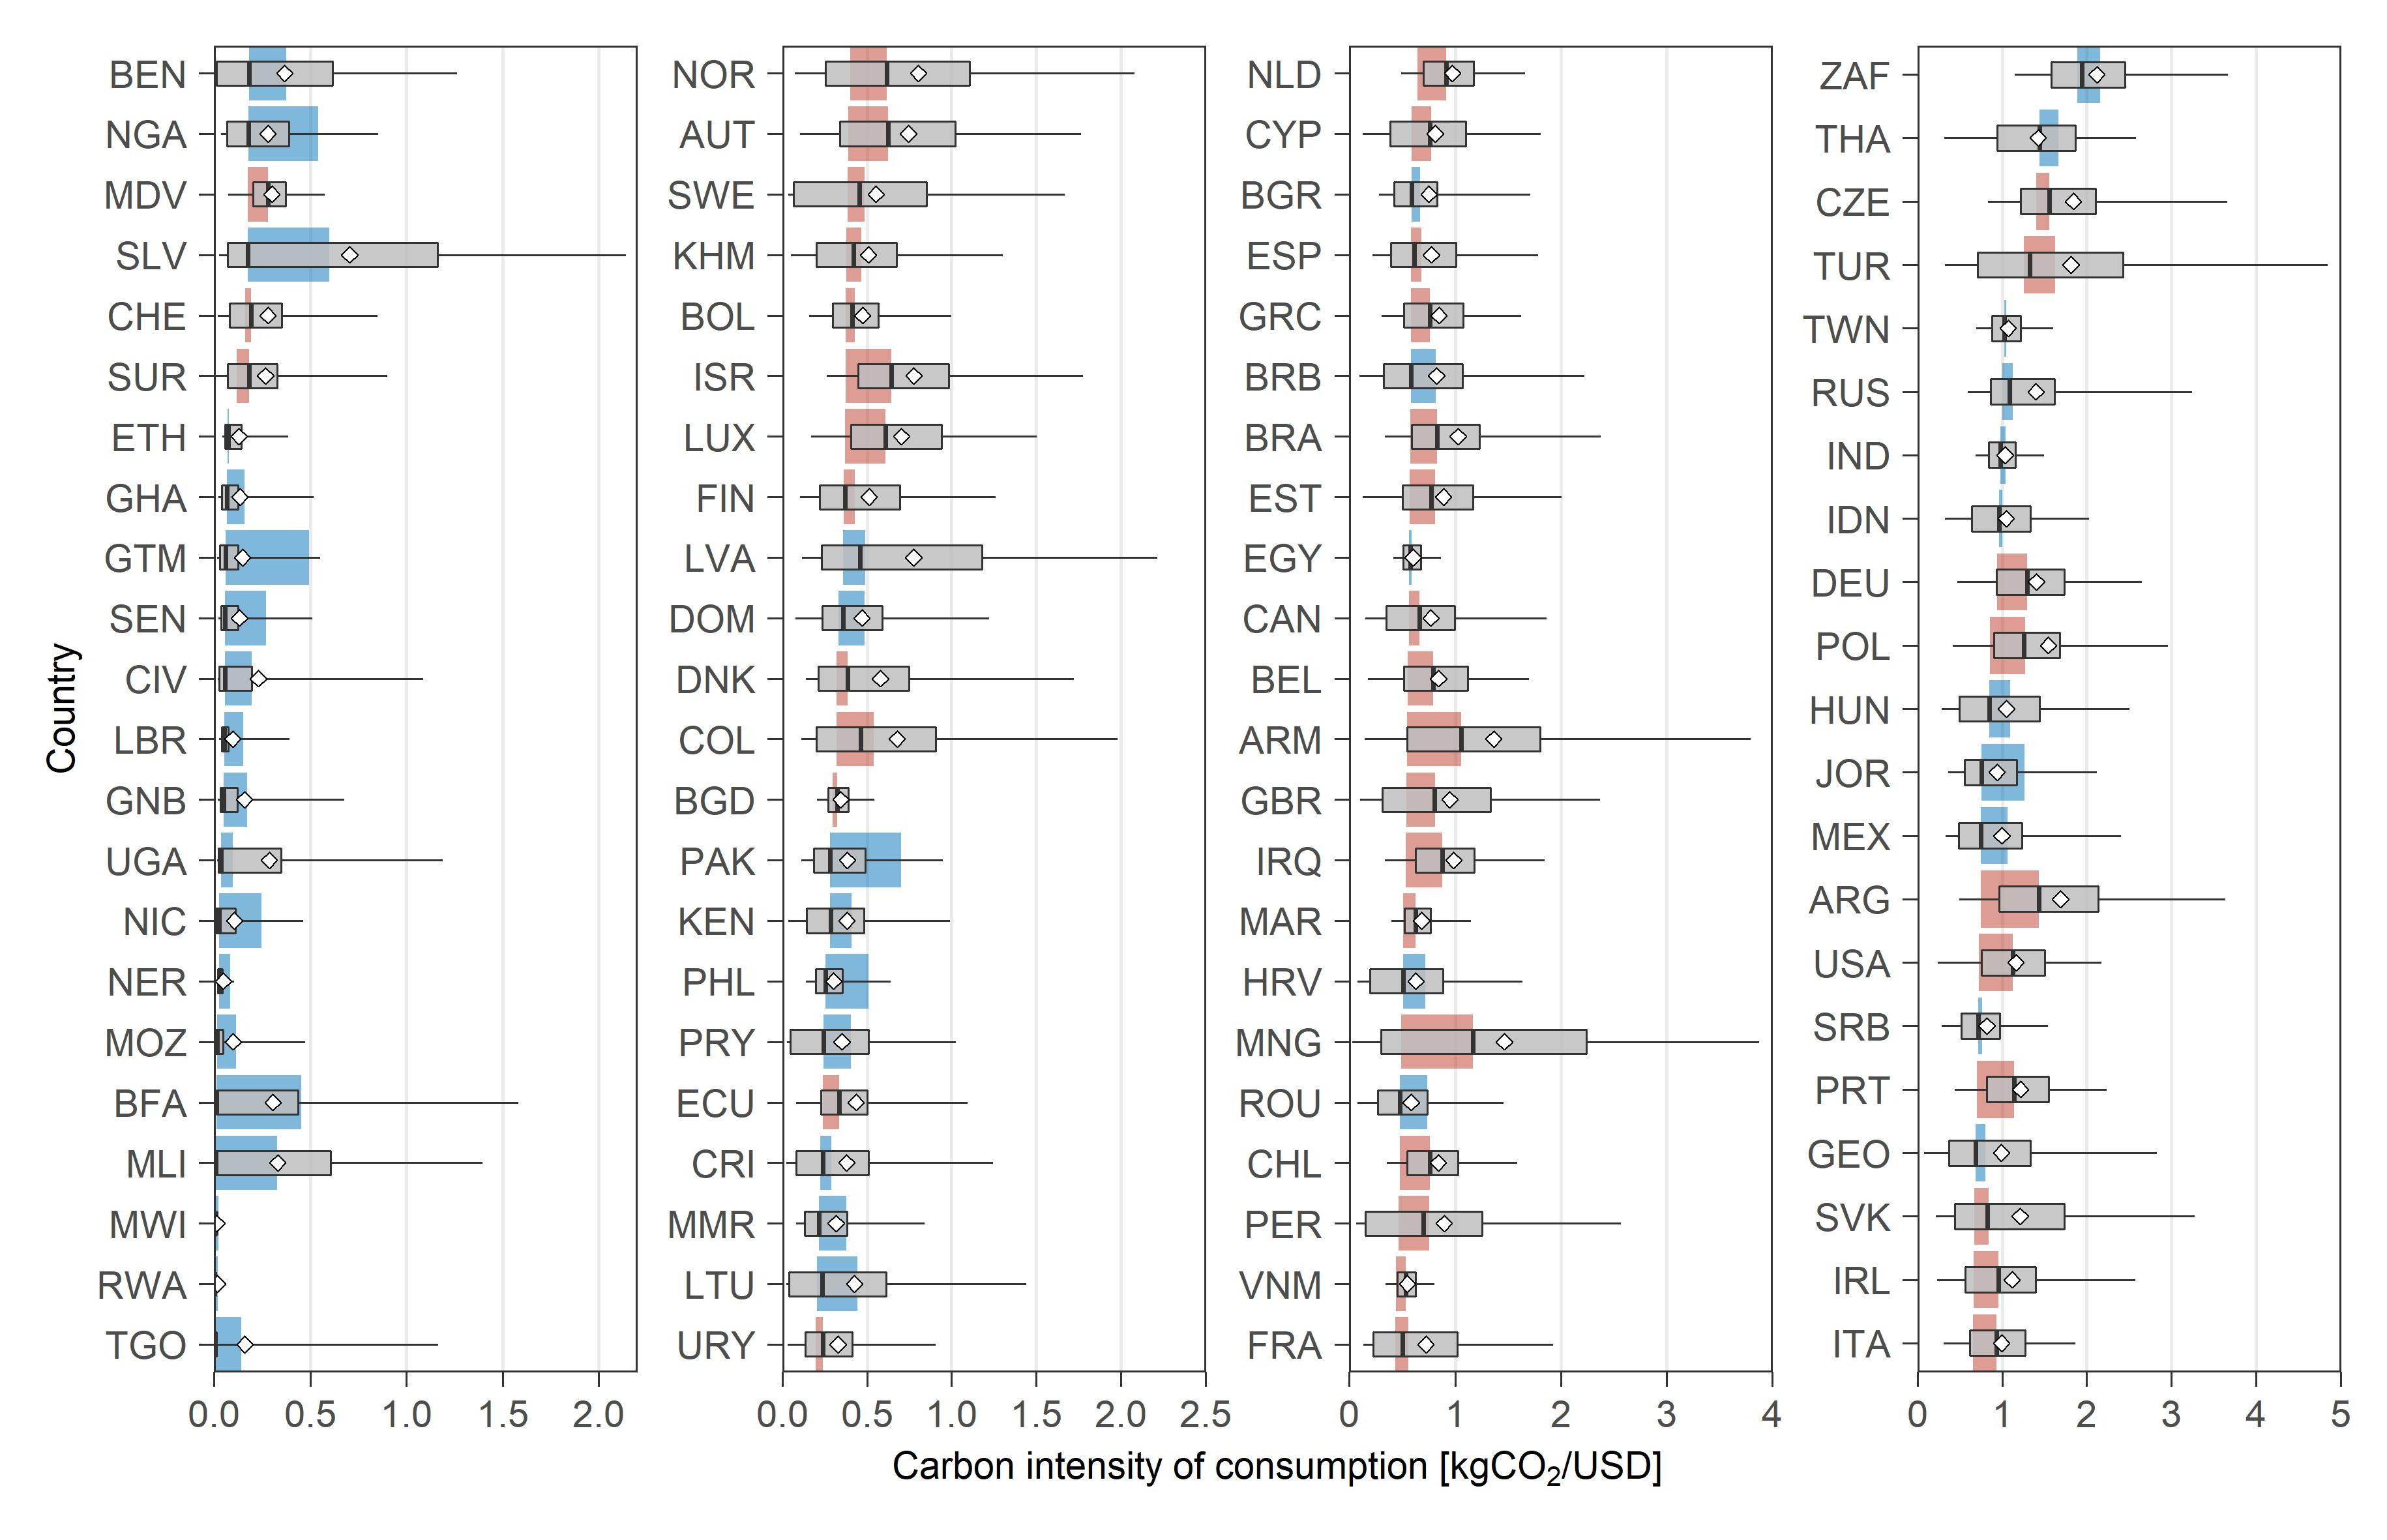
\includegraphics{Figure 1/Figure_1_2017}
    \caption{Vertical differences and distribution of carbon intensity within poorest quintiles}
    \label{fig:fig_1}
    \begin{subcaption2}
    Boxplots display the distribution of household-level carbon intensity within the poorest quintile in each of 87 countries: The boxes display the $25^{th}$ and $75^{th}$ percentile; whiskers display the $5^{th}$ and $95^{th}$ percentile, respectively. Rhombuses display the mean. Blue and red bars represent the vertical difference in household-level carbon intensity, i.e., the difference between the highest and the lowest median carbon intensity across quintiles. Blue (red) bars indicate that the average carbon intensity is higher (lower) in richer households compared to poorer households. See also Figures \ref{fig:Quint_A} to \ref{fig:Quint_C}.
    \end{subcaption2}
\end{figure}

Figure \ref{fig:fig_1} illustrates that within-quintile heterogeneity exceeds between-quintile differences in \textit{all} countries\footnote{See Figures \ref{fig:Quint_A} to \ref{fig:Quint_C} for country-level comparisons across all expenditure quintiles and Table \ref{tab:A3} for summary statistics on carbon footprints and carbon intensity of consumption.}. This underlines that analyses building on differences in income to explain differences in carbon intensity of consumption (or the impact of climate policy) might be insufficient since it falls short of accounting for differences in carbon intensity at similar levels of income. Instead, we propose including household-level characteristics beyond income in such analyses to give a more nuanced description of which households' consumption is especially carbon-intensive.

This is also warranted, because - as we show in Figure \ref{fig:fig_2} - within-quintile differences vary across quintiles. To facilitate comparison across countries, we compute two coefficients \autocite{Missbach.2024}: The vertical distribution coefficient $\overline{V_{r}}$ compares median carbon intensity of the poorest and the richest expenditure quintile:

\begin{equation}
    \widehat{V_{r}} = \frac{\overline{e_{EQ1}}}{\overline{e_{EQ5}}}
\end{equation}

If median carbon intensity among poorer households exceeds (is smaller than) the median carbon intensity of richer households, then $\widehat{V_{r}}>1$ ($\widehat{V_{r}}<1$) and climate policy would likely lead to \textit{regressive} (\textit{progressive}) outcomes.

The horizontal distribution coefficient $\overline{H_{r}}$ compares within-quintile differences of the poorest and the richest expenditure quintile:

\begin{equation}
    \widehat{H_{r}} = \frac{e_{EQ1}^{95} - e_{EQ1}^{5}}{e_{EQ5}^{95} - e_{EQ5}^{5}}
\end{equation}

$\widehat{H_{r}}>1$ ($\widehat{H_{r}}<1$) would indicate that within-quintile differences are larger (smaller) among poorer compared to richer households.

Figure \ref{fig:fig_2} illustrates that the average carbon intensity of consumption is larger among the poorest quintile in 43 out of 87 countries compared to the richest quintile. These countries have a higher GDP per capita than others: We observe $\widehat{V_{r}}>1$ for 20 out of 20 countries in our sample with the highest GDP per capita. In these countries, climate policies (such as carbon pricing) are likely to have regressive effects. Similarly, carbon intensity is higher for richer quintiles compared to poorer quintiles ($\widehat{V_{r}}<1$ ) in 18 out of 20 countries in our sample with the lowest GDP per capita. This is in line with inverse-U-shaped Engel curves for carbon-intensive goods and services across countries and income quintiles \autocite{Dorband.2019}. %Interestingly, this does not necessarily hold in each single country.

\begin{figure}[ht!]
    \centering
    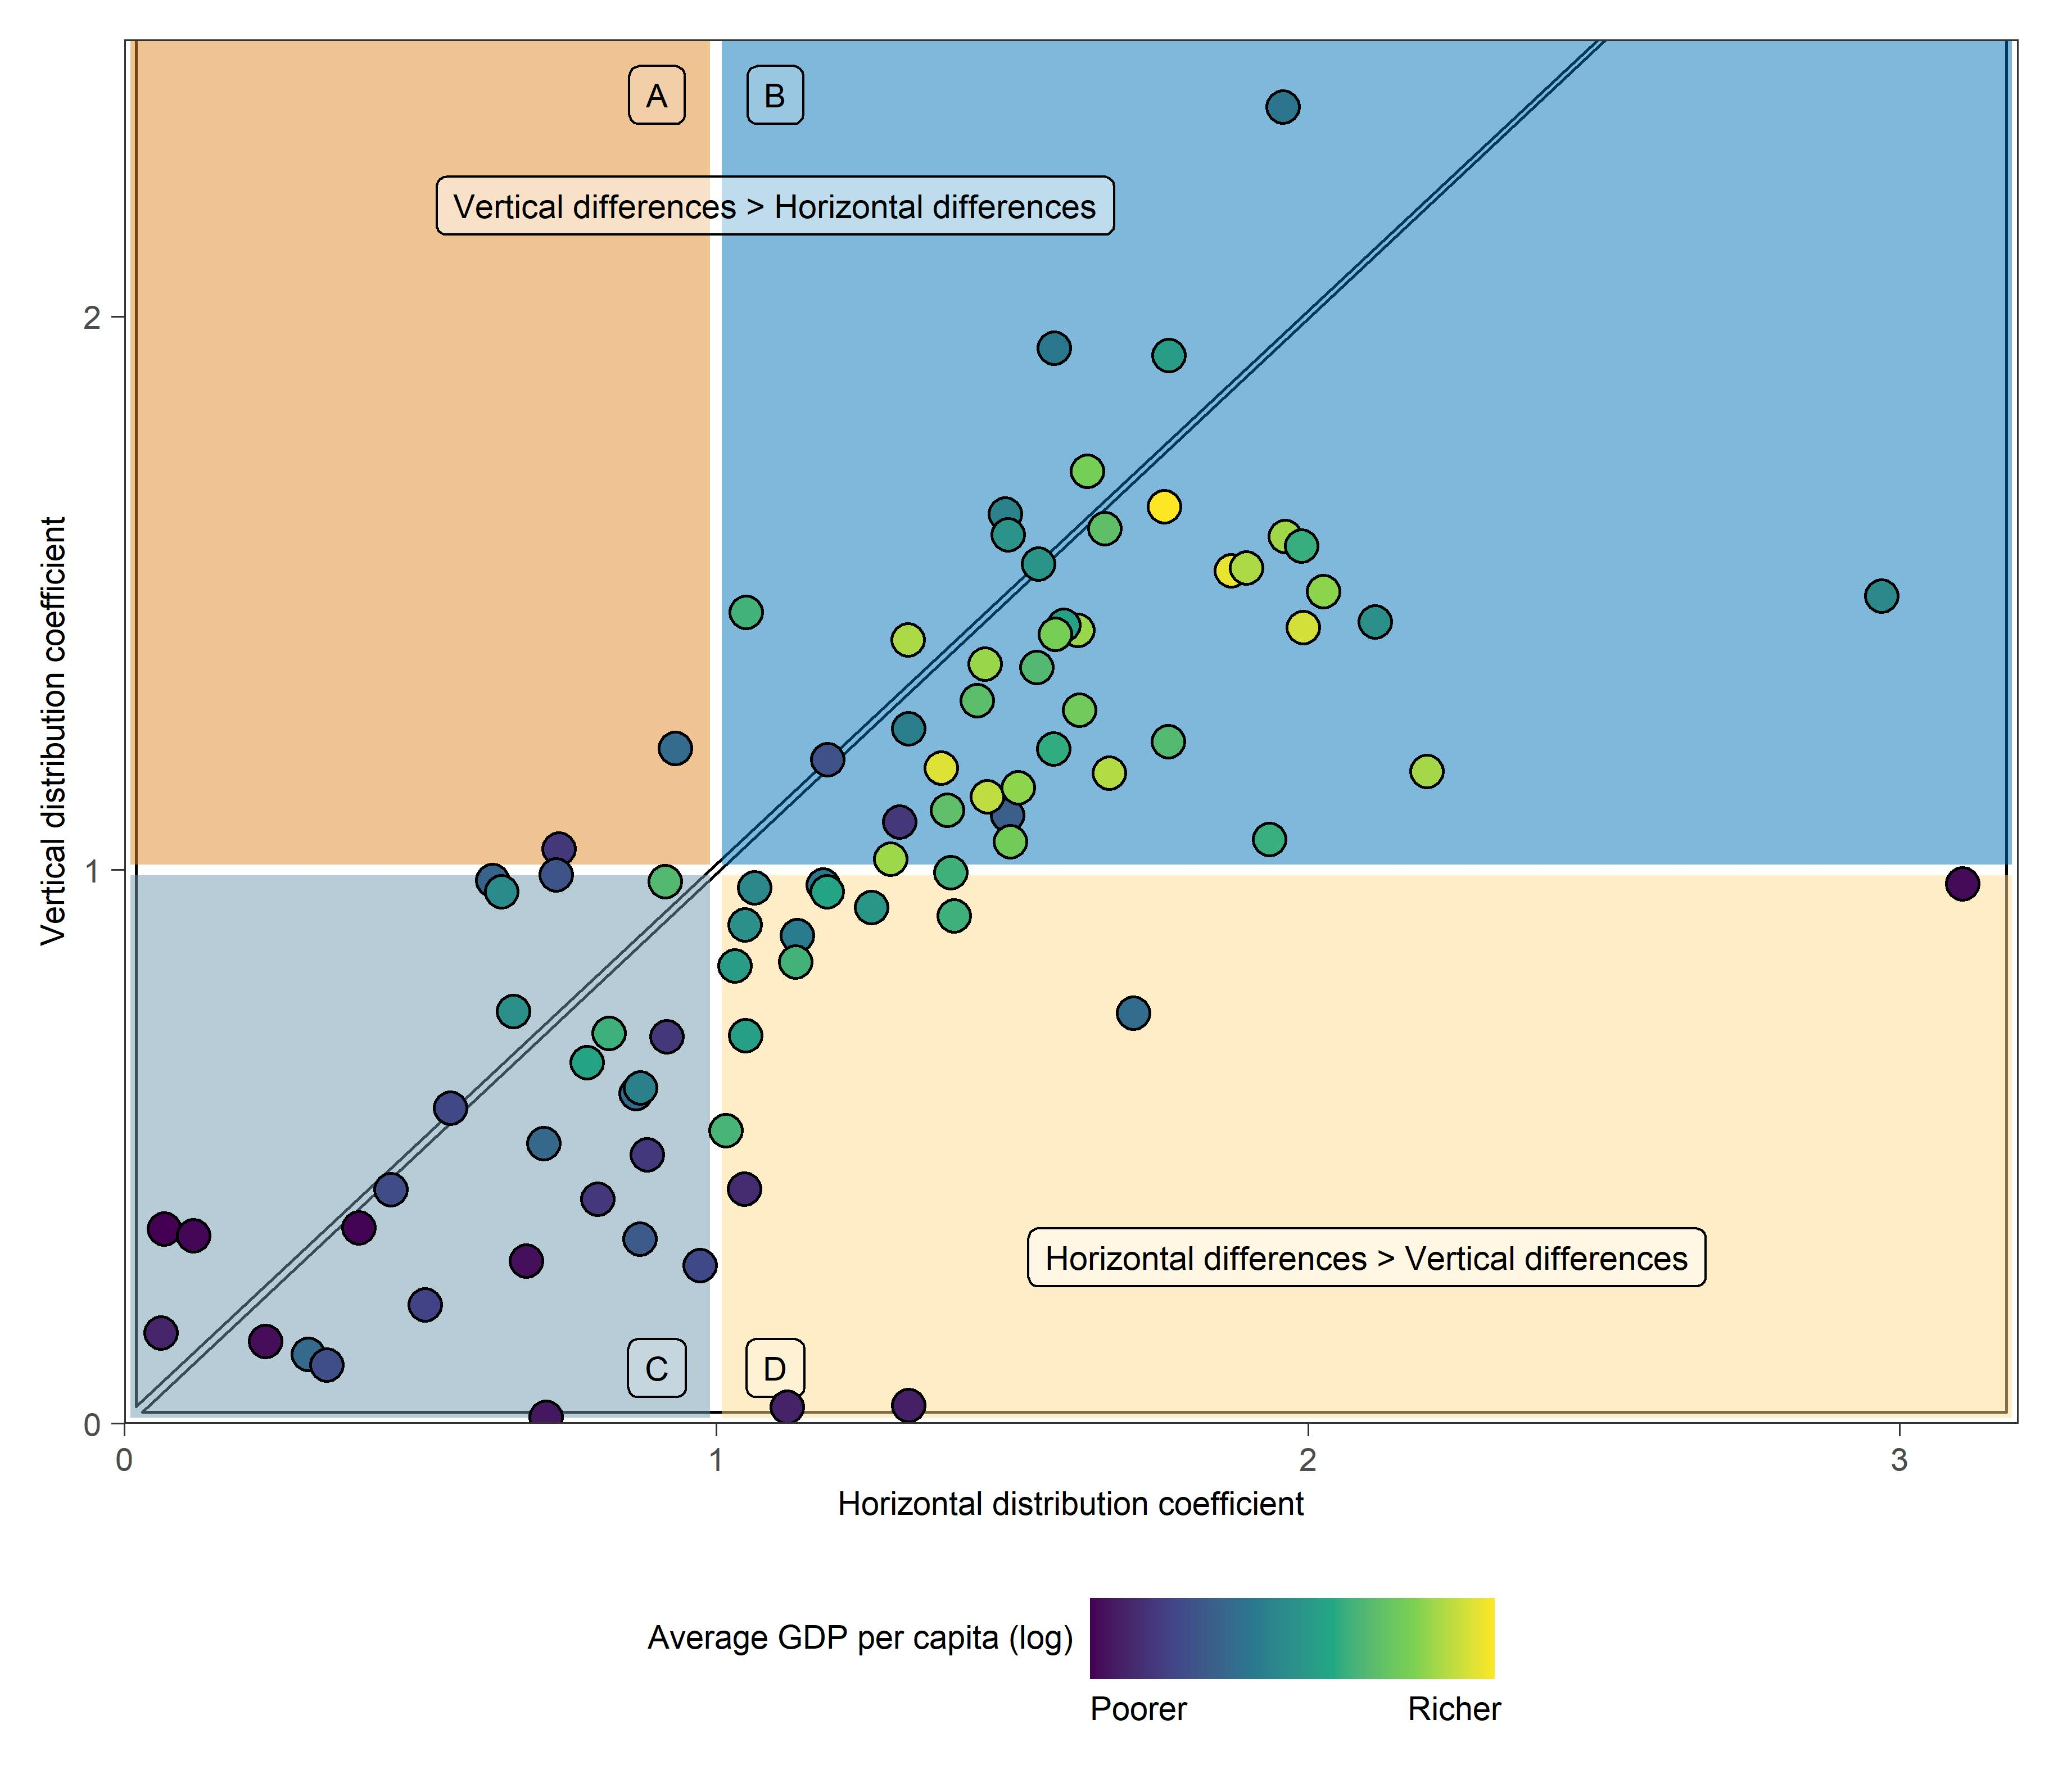
\includegraphics{Figure 2/Figure_2_2017}
    %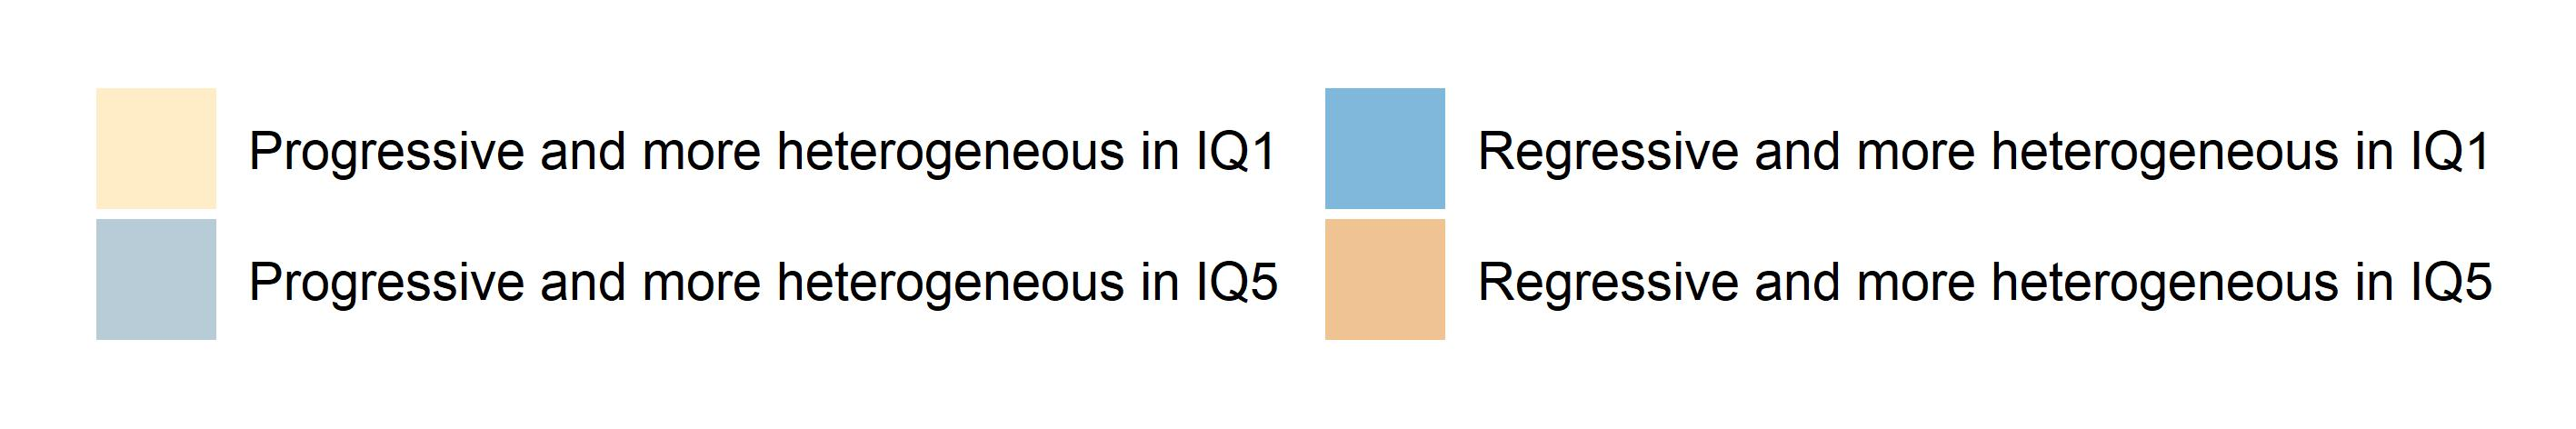
\includegraphics{Figure 2/Legend}
    \caption{Vertical and horizontal distribution coefficient}
    \label{fig:fig_2}
    \begin{subcaption2}
    The vertical distribution coefficient compares the median carbon intensity of the richest to the poorest quintile. The horizontal distribution coefficient compares the within-quintile differences ($5^{th}$ to $95_{th}$ percentile within quintiles) of the richest to the poorest quintile. Rectangles (A) and (B) indicate higher carbon intensity (at the median) among the poorest quintile compared to the richest quintile; rectangles (C) and (D) indicate lower carbon intensity (at the median) among the poorest quintile compared to the richest quintile. Rectangles (A) and (C) indicate smaller within-quintile differences of carbon intensity among the richest quintile compared to the poorest quintile; rectangles (B) and (D) indicate larger within-quintile differences of carbon intensity among the richest quintile compared to the poorest quintile. Colors of points indicate GDP per capita for 2018 (in log-transformed constant 2010 US-\$). See also Table \ref{tab:A7}.
    \end{subcaption2}
\end{figure}

% Check all numbers
In 58 out of 87 countries, within-quintile variation (expressed as the difference at the $5^{th}$ and the $95^{th}$ percentile within quintiles) is larger in the poorest quintile compared to the richest quintile. Horizontal differences, i.e. within-quintile heterogeneity, exceed vertical differences, i.e. between-quintile heterogeneity in 66 countries, emphasizing the need for detailed investigation of household characteristics associated to higher levels of carbon intensity of consumption.

In response, one core assumption of this study is that $e_{i}$, the carbon intensity of household \textit{i}, correlates with observable household characteristics $X_{i}^{'}$:

\begin{equation}
    e_{i} \sim X_{i}^{'}
\end{equation}

% Which criteria should be included in modelling and why?
% Discuss main arguments for single characteristics (possibly already in methods section).

To shed light on which household characteristics correlate with and lead to higher levels of carbon intensity of consumption we build on two modeling approaches, namely boosted regression trees (BRT) and a logit-model.

\paragraph{Boosted regression trees} Fitting boosted regression trees (BRT) \autocite{Friedman.2003, Elith.2008} is a supervised machine learning method allowing for detection of non-linear relationships and interaction effects between an outcome and many predictor variables (features). As an extension to regression trees, the BRT algorithm (\textit{XGBoost} \autocite{Chen.2016}) fits many single regression trees, iteratively giving higher weights to observations with larger predicting errors. This leads to large predictive power, also if compared to the frequently used random forest algorithm. Nevertheless, fitting BRT is more computationally intensive and outcomes are more difficult to interpret compared to outcomes from other machine learning models. % Why BRT is helpful here.

Drawing on BRT serves the purpose of our analysis, because it is a priori ambiguous which variables to include in a model. In addition, research indicates that the impacts of climate policy (and therefore the carbon intensity of consumption) distribute non-linearly across households with different characteristics, such as income, demographic groups \autocite{Missbach.2023}, energy use \autocite{Farrell.2017} and space \autocite{Chan.2023}. In contrast to other approaches, such as variance-based inequality decomposition \autocite{Farrell.2017,Sager.2019b,Missbach.2024}, using BRT is well-suited to help identifying important predictors while also allowing for detection of potentially non-linear relationships.

We fit BRT-models on the country-level to investigate characteristics associated to heterogeneous levels of carbon intensities within single countries. The carbon intensity $e_{i}$ is the outcome variable. For each country-level model we use the entire set of observable household-level characteristics $X_{i}^{'}$ as possible features and perform several feature engineering steps (see also Appendix \ref{sec:featureengineering}).

The predictive performance of BRT-models critically hinges on several hyperparameters. For hyperparameter tuning, we randomly split country-level data into a training and a test sample, comprising 80\% and 20\% of observations, respectively. We use five-fold cross-validation on the training sample to fit 1,000 trees - following the recommendations by \textcite{Elith.2008} - along with 30 different combinations of learning rate ($\eta \in [0.001,0.3]$), the maximum depth of trees (\textit{max\_depth} $\in \{x \in \mathbb{N} \mid 1  \leq x \leq 15 \}$) and a fraction of features included in each tree (\textit{mtry} $\in \{0.5,0.7,1\}$). We select combinations of hyperparameters such that combinations distribute evenly across the possible combination space. For each country, we select the combination of hyperparameters that minimizes mean absolute error.

Building on selected hyperparameters, we use five-fold cross-validation on all observations, i.e., from the training and test sample, for model evaluation. We evaluate model performance with the help of mean absolute error (MAE), root mean squared error (RMSE) and goodness of fit ($R^{2}$). We also use all observations to evaluate the relative importance of each feature with the help of SHAP-values: SHAP-values represent the contribution of each feature to each individual prediction and have been proposed as a more suitable means to interpret outcomes of machine learning models compared to other approaches \autocite{Lundberg.2020}. We also determine feature importance by calculating the average absolute SHAP-value for each feature across all individual predictions. We show feature importance as a share of contribution (in \% of total mean absolute SHAP-values) to allow for better comparability of feature importance across countries. We visualize the distribution of SHAP-values for the most important features in each country over feature values, i.e., in partial dependence plots. 

\paragraph{Logit-model} For supplementary robustness analyses, we also fit a logit-model to identify households whose consumption is relatively more carbon-intensive compared to the entire population. We construct a binary variable $e_{i}^{80^{th}}$ for each household \textit{i} indicating whether the household is among the most carbon-intensive 20\% of households in each country:

\begin{equation}
    e_{i}^{80^{th}} =
    \begin{cases}
    1, & \text{for }  e_{i} \geq e^{80^{th}} \\
    0, & \text{for }  e_{i} < e^{80^{th}}
    \end{cases}
\end{equation}

Subsequently, be $P_{e_{i}^{80^{th}}}$ the probability of household \textit{i} to consume more carbon-intensively than 80\% of the population in each country. We are interested in the coefficients $\beta^{'}$ of the following logit-model:

\begin{equation}
    log \left( \frac{P_{e_{i}^{80}}}{1 - P_{e_{i}^{80}}} \right) = \alpha_{0} + \beta^{'} X_{i}^{'} + \varepsilon_{i}
\end{equation}

Estimating a logit-model serves as a robustness check for results from BRT-models. It also allows for investigation of characteristics associated to "hardship-case" households including a more accessible interpretation of results and parameters. We show results from logit-models with the help of regression tables and visualize average marginal effects for each independent variable.

\paragraph{Identifying country clusters} Country-level analyses can be meaningful to identify country-specific household characteristics associated to higher levels of carbon intensity of consumption. In fact, the relationship between household-level characteristics and carbon intensity of consumption is unique for each country, but also contingent on the availability of granular data. To account for differences in available features across countries, we adjust individual feature importance by multiplying individual feature importance and country-level $R^{2}$. This approach also helps to account for the aggregate performance of country-level models and allows for better comparison of feature importance across countries.

Building on (adjusted) feature importance for each country, we use k-means clustering algorithm to learn more about which features are more important in many countries. If features are missing in the data, we assume their share of contribution is zero. We normalize all feature values to allow for comparison across features. If one feature is more (less) important in one country compared to all other countries, the processed feature value will be relatively high (low). If one feature is equally important across all countries, processed feature values will be close to zero.

K-means clustering is an unsupervised machine-learning method and helps to analyze clusters of observations that are most similar in many variables within each cluster and least similar in many variables across clusters \autocite{MacQueen.1967}. We inspect the optimal number of clusters ($\{k \in \mathbb{N} \mid 2  \leq k \leq 20 \}$) with the help of average silhouette widths \autocite{Rousseeuw.1987} for each cluster \textit{k}. The silhouette width $s_{i}$ accounts for the average Euclidean distance of each observation \textit{i} to all other observations within its cluster and for the average distance to observations from the nearest neighbouring cluster. Silhouettes closer to $1$ indicate a good fit of an observation to its cluster and silhouettes closer to $-1$ indicate a poor fit. The average silhouette width $\overline{s_{k}}$ for each cluster \textit{k} expresses how well all observations fit on average to each cluster. Our approach yields $k = 9$ to be the number of clusters maximizing average silhouette width\footnote{See Figures\ref{fig:G1_silhouette} and \ref{fig:G2_silhouette} for visualization.}. We also show the optimal number of clusters ($k = 15$) for k-means clustering building on non-adjusted feature importance in the Appendix\footnote{See Figures \ref{fig:G3_silhouette_2} and \ref{fig:G4_silhouette_2} for visualization. Using non-adjusted feature importance for clustering changes the interpretation of clusters: Features of countries within the same cluster contribute similarly to explaining variation in carbon intensity without respecting the availability of features in the data and the explanatory power of the model.}.

In countries within the same clusters single features are similarly important to predict the carbon intensity of households. For each country-cluster, we compute average values for each feature to allow for investigation of differences between countries in different clusters. We also investigate which country is most likely to all other countries in each cluster maximizing silhouette width within each cluster and use it to demonstrate cluster-level characteristics. 

It is important to note that our approach to adjust feature values for total model performance reduces in the influence of feature availability in the data for clustering. Uncorrected feature importance values may be exaggerated, if only few features exist, so countries with few features may end up in wrong clusters mainly because the model cannot help explaining much of the variation in carbon intensity. Instead, our approach ensures that all \textit{observable} features contribute to clustering. Despite many structurally unobservable household-level features, our approach might be warranted under the assumption that policy formulation (for example on optimal targeting of compensation measures) can naturally only center on observable characteristics, if targeting errors should be minimized.

\begin{itemize}
    \item Methodological discussion (brief) ?
    %\item Analyzing vertical inequality
    %\item Analyzing horizontal inequality
    %\item Introduce boosted regression trees
    %\item Introduce logit model as robustness check, supplementary analysis
    %\item Critical appraisal
\end{itemize}

\clearpage

\section{Results: Heterogeneity of carbon intensity of consumption} \label{sec:results}

Climate policy can lead to short-term costs distributing unevenly across the population according to heterogeneous household-level carbon intensity of consumption. The carbon intensity of households correlates with household characteristics, including - but not limited to - total household expenditures. In the following, we present an analysis of a set of household characteristics and their importance for predicting the carbon intensity of households. We compare results across countries and assign countries to clusters. Lastly, we assess the heterogeneity of carbon intensities with different regional and sectoral coverage.

\paragraph{Model accuracy} As we show in Table \ref{tab:A8}, fitting BRT-models helps to predict households' carbon intensity with good precision in many countries. Models' goodness of fit ($R^{2}$) accumulates to 59\% for Jordan, 53\% for Peru and 50\% for Nicaragua and Niger. For 28 countries, $R^{2}$ exceeds 30\%. For some countries, however, our models yield relatively low predictive performance: For 18 countries, $R^{2}$ does not exceed 10\%. Model performance is lowest in Bulgaria (1\%), Estonia (2\%), Serbia (3\%) and Suriname (3\%). One reason is that performance hinges critically on data granularity. For many countries with low predictive performance our model is restricted to drawing on few available features, such as household expenditures, sub-national area identifiers, household size or education of household head.

Low model accuracy in some countries implies that it is difficult to infer about the carbon intensity of households through observable characteristics, such as household expenditures. In Bulgaria, for example, vertical differences are low and horizontal differences within expenditure quintiles are large (Figure \ref{fig:Quint_C}). Moreover, as our analysis confirms, within-quintile variation in total expenditures is largely uncorrelated with variation in carbon intensity. In such contexts, compensation measures based on expenditures of households (such as reducing consumption taxes) would likely benefit all households equally, but prove ineffective to compensate households with highest costs.

\paragraph{Country-level feature importance}

The importance of features differs across countries. Figure \ref{fig:fig_4_1}, Figure \ref{fig:fig_4_2} and Table \ref{tab:A10} show our indicators for vertical and horizontal inequality, the mean CO$_{2}$-intensity and adjusted feature importance for all features in each country, grouped by country clusters. %Describe single clusters, at least A, B, C and D. Touch briefly upon the rest.
% What are important features? In which direction? Why?

Figure \ref{fig:5b} shows partial dependence plots for all countries and each cluster, visualizing differences in SHAP-values, i.e. the contribution to predicted carbon intensity of consumption for different feature values. While feature importance helps to identify features explaining heterogeneity in carbon intensity, the distribution of SHAP-values indicates the (non-linear) relationships between features and outcome variable.

On average, the most important feature across countries is household expenditures, accounting for a relative contribution of 22\% on average. Household expenditures are the single most important feature for prediction in 30 countries, and in some countries, such as \hyperref[fig:5b_LUX]{Luxembourg} or \hyperref[fig:5b_HRV]{Croatia}, differences in household expenditures contribute to more than 50\% of model predictions. Household expenditures account for largest shares of adjusted feature importance in \hyperref[fig:5b_PER]{Peru} (18\%), \hyperref[fig:5b_ECU]{Ecuador} (14\%) and \hyperref[fig:5b_IRQ]{Iraq} (14\%) - countries in which we also identify strictly larger carbon intensities for poorer households compared to richer households. The relationship between expenditures and carbon intensity is non-linear, but overall declining for 53 countries (e.g. \hyperref[fig:5b_EST]{Estonia}), increasing for 14 countries (e.g. \hyperref[fig:5b_GHA]{Ghana}), following an U-shape for 5 countries (e.g. \hyperref[fig:5b_IND]{India}) and an inverse-U-shape for 11 countries (e.g. \hyperref[fig:5b_TUR]{Turkey}). We find declining relationships between household expenditures and carbon intensity for 19 of 20 countries with highest GDP per capita, which lends credibility to our prior analysis in section \ref{sec:methods}. Under such circumstances, more carbon-intensively consuming households spend less on consumption, but relatively more on carbon-intensive goods and services. Compensation measures based on expenditures of households can be effective to compensate households with highest costs.

Motorcycle and car ownership is the most important feature in 15 and 14 countries, respectively. In \hyperref[fig:5b_BFA]{Burkina Faso}, \hyperref[fig:5b_MLI]{Mali}, \hyperref[fig:5b_NER]{Niger} or \hyperref[fig:5b_TGO]{Togo} variation in motorcycle ownership can be attributed to more than 20\% of variation in carbon intensity. Car ownership accounts for largest adjusted feature importance in \hyperref[fig:5b_JOR]{Jordan} (33\%) and \hyperref[fig:5b_TWN]{Taiwan} (25\%). Vehicle ownership is the most important adjusted feature across all countries and features and can be a meaningful predictor for predicting climate policy impacts in some countries: Households owning motorcycles or cars are more likely to consume more carbon-intensively than households without such vehicles in every country of our sample. This links to the propensity of vehicle-owning (and -using) households to consume relatively more transport fuels than others.

Spatial features, such as urban or rural location, state, province or district of household, are the most important features in 17 countries. For example, urban citizenship contributes more than 40\% of model prediction in countries such as \hyperref[fig:5b_CZE]{Czech Republic}, \hyperref[fig:5b_SVK]{Slovakia} or \hyperref[fig:5b_LVA]{Latvia}. We find urban households to consume less carbon-intensively compared to rural households in a majority of countries such as \hyperref[fig:5b_FRA]{France}, \hyperref[fig:5b_NOR]{Norway}, \hyperref[fig:5b_ESP]{Spain}, and more carbon-intensively in countries such as \hyperref[fig:5b_MNG]{Mongolia}, \hyperref[fig:5b_PAK]{Pakistan} or \hyperref[fig:5b_ROU]{Romania}. For \hyperref[fig:5b_IND]{India}, where state residence accounts for adjusted feature importance of 8\%, we document that households in Jharkand, West Bengal or Manipur consume more carbon-intensively than households in Pondicherry, Haryana or Sikkim. In \hyperref[fig:5b_BOL]{Bolivia}, where department residence accounts for adjusted feature importance of 6\%, households in Pando or Cochabamba consume more carbon-intensively than households from Potosí or Chuquisaca. Carbon intensity differences across space hint towards the important role of access to energy and transport infrastructure. For example, in cities, households may choose from different transport modes including public transportation. 

Features describing energy use, such as main fuels used for cooking, lighting and heating, or electricity access and appliance ownership are the most important feature in eight countries. Main cooking fuel is an important feature in \hyperref[fig:5b_PER]{Peru} and \hyperref[fig:5b_NIC]{Nicaragua} with adjusted feature importance of 18\% and 16\%, respectively. In both countries, households cooking with LPG consume substantially more carbon-intensive than households cooking predominantly with firewood, a pattern that is consistent in all countries with a non-negligible share of households using firewood or charcoal. This result is consistent with our assumption of zero direct emissions for biomass, firewood or charcoal, because of informal markets and structural difficulties to regulate (and tax) such emissions. Using kerosene for lighting is associated to higher carbon intensity compared to electricity and other lighting source in \hyperref[fig:5b_UGA]{Uganda}, \hyperref[fig:5b_RWA]{Rwanda} or \hyperref[fig:5b_ETH]{Ethiopia}. Information on heating fuels exists only in few countries, but is the single most important feature in \hyperref[fig:5b_TUR]{Turkey} and \hyperref[fig:5b_ARM]{Armenia}. Carbon intensity is higher in households heating with coal (\hyperref[fig:5b_TUR]{Turkey}) or natural gas (\hyperref[fig:5b_ARM]{Armenia}) compared to households heating with electricity.

Electricity access is a relatively less important feature, contributing a maximum of 4\% of adjusted feature importance in \hyperref[fig:5b_SEN]{Senegal}. In a majority of countries, feature importance for electricity access is low, possibly because of overall high (e.g. \hyperref[fig:5b_VNM]{Vietnam}, \hyperref[fig:5b_PHL]{Philippines}) or low electricity access rates (e.g. \hyperref[fig:5b_MWI]{Malawi}, \hyperref[fig:5b_LBR]{Liberia}) or because of low CO$_{2}$-intensity in the electricity sector (e.g. \hyperref[fig:5b_ETH]{Ethiopia}, \hyperref[fig:5b_KEN]{Kenya}).

Instead, ownership of major household appliances (such as refrigerators, washing machines or air conditioning) is the most important feature in \hyperref[fig:5b_CHE]{Switzerland} and the \hyperref[fig:5b_PHL]{Philippines}, contributing 17\% of adjusted feature performance in the Philippines. This is less surprising, because appliance ownership is a more compelling, yet incomplete proxy for electricity \textit{use} compared to electricity \textit{access}.

Sociodemographic features, such as education, are the most important feature in three countries. In \hyperref[fig:5b_PRT]{Portugal}, where education of household accounts for 29\% of model prediction, households with tertiary education exhibit a higher carbon intensity than households with primary or secondary education. Adjusted feature importance for features such as gender of household head, self-identified ethnicity, language or religion is highest in \hyperref[fig:5b_BEN]{Benin} or \hyperref[fig:5b_TGO]{Togo}, where households with female household heads are found to consume less carbon-intensively. In \hyperref[fig:5b_ISR]{Israel}, households identifying with the Muslim community are found to consume more carbon-intensively compared to households identifying as Jewish. Traditional, religious and orthodox households' carbon intensity is larger compared to secular households. For 71 out of 87 countries, sociodemographic features do not exceed 3\% of adjusted feature importance, indicating their relatively low relevance across countries.

\begin{figure}[ht!]
    \centering
    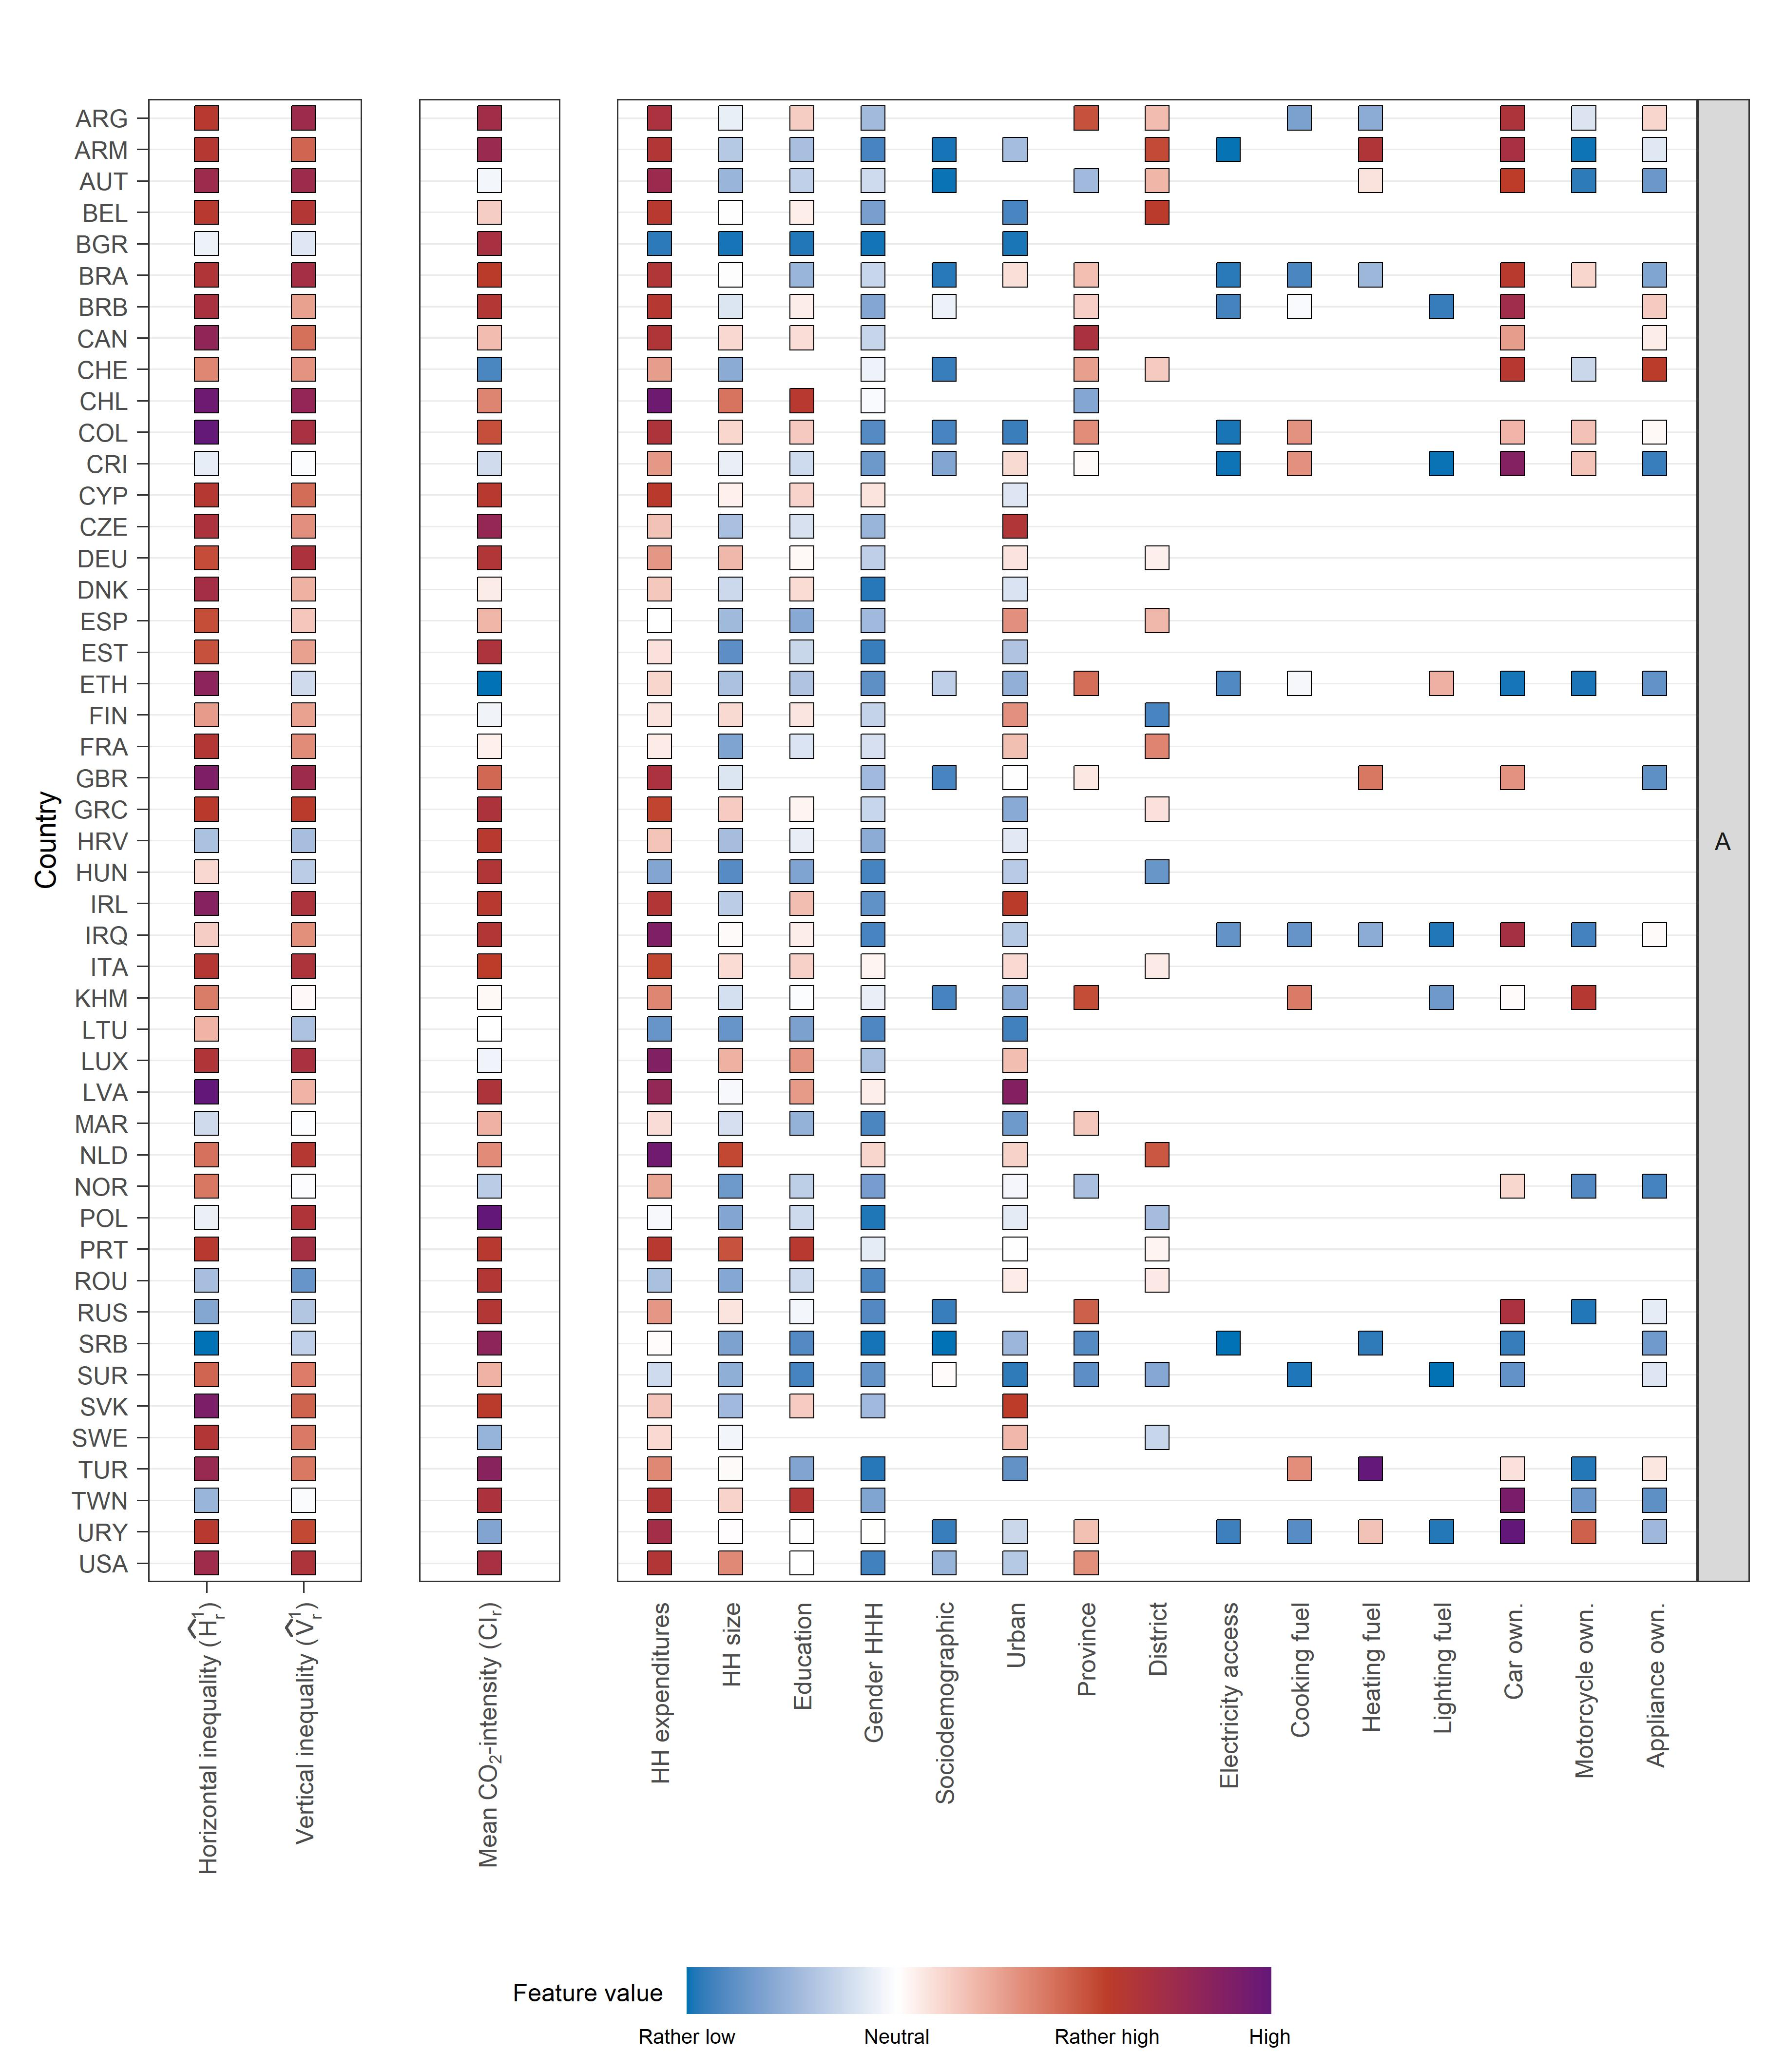
\includegraphics{1_Figures/Figure 4/Figure_4_Corrected_1.jpg}
    \caption{Feature importance across countries by cluster}
    \label{fig:fig_4_1}
    \begin{subcaption2}
    This figure shows the importance of features (in normalized average absolute SHAP-values) for each country, grouped by country clusters. Blue (red) colors indicate that a feature is relatively less (more) important in a country compared to all other countries. 'Sociodemographic' comprises normalized absolute SHAP-values for features such as ethnicity, nationality, religion or language.
    For horizontal inequality, blue (red) colors indicate a lower (higher) heterogeneity within the first income quintile compared to the fifth income quintile. For vertical inequality, blue (red) colors indicate lower (higher) median carbon intensity among the first income quintile compared to the fifth income quintile. For average CO$_{2}$-intensity, blue (red) colors indicate a lower (higher) average carbon intensity across all countries.
    We assign countries to 9 clusters performing k-means clustering based on scaled values across all features. We also show all values in Table \ref{tab:A10}.
    \end{subcaption2}
\end{figure}

\begin{figure}[ht!]
    \centering
    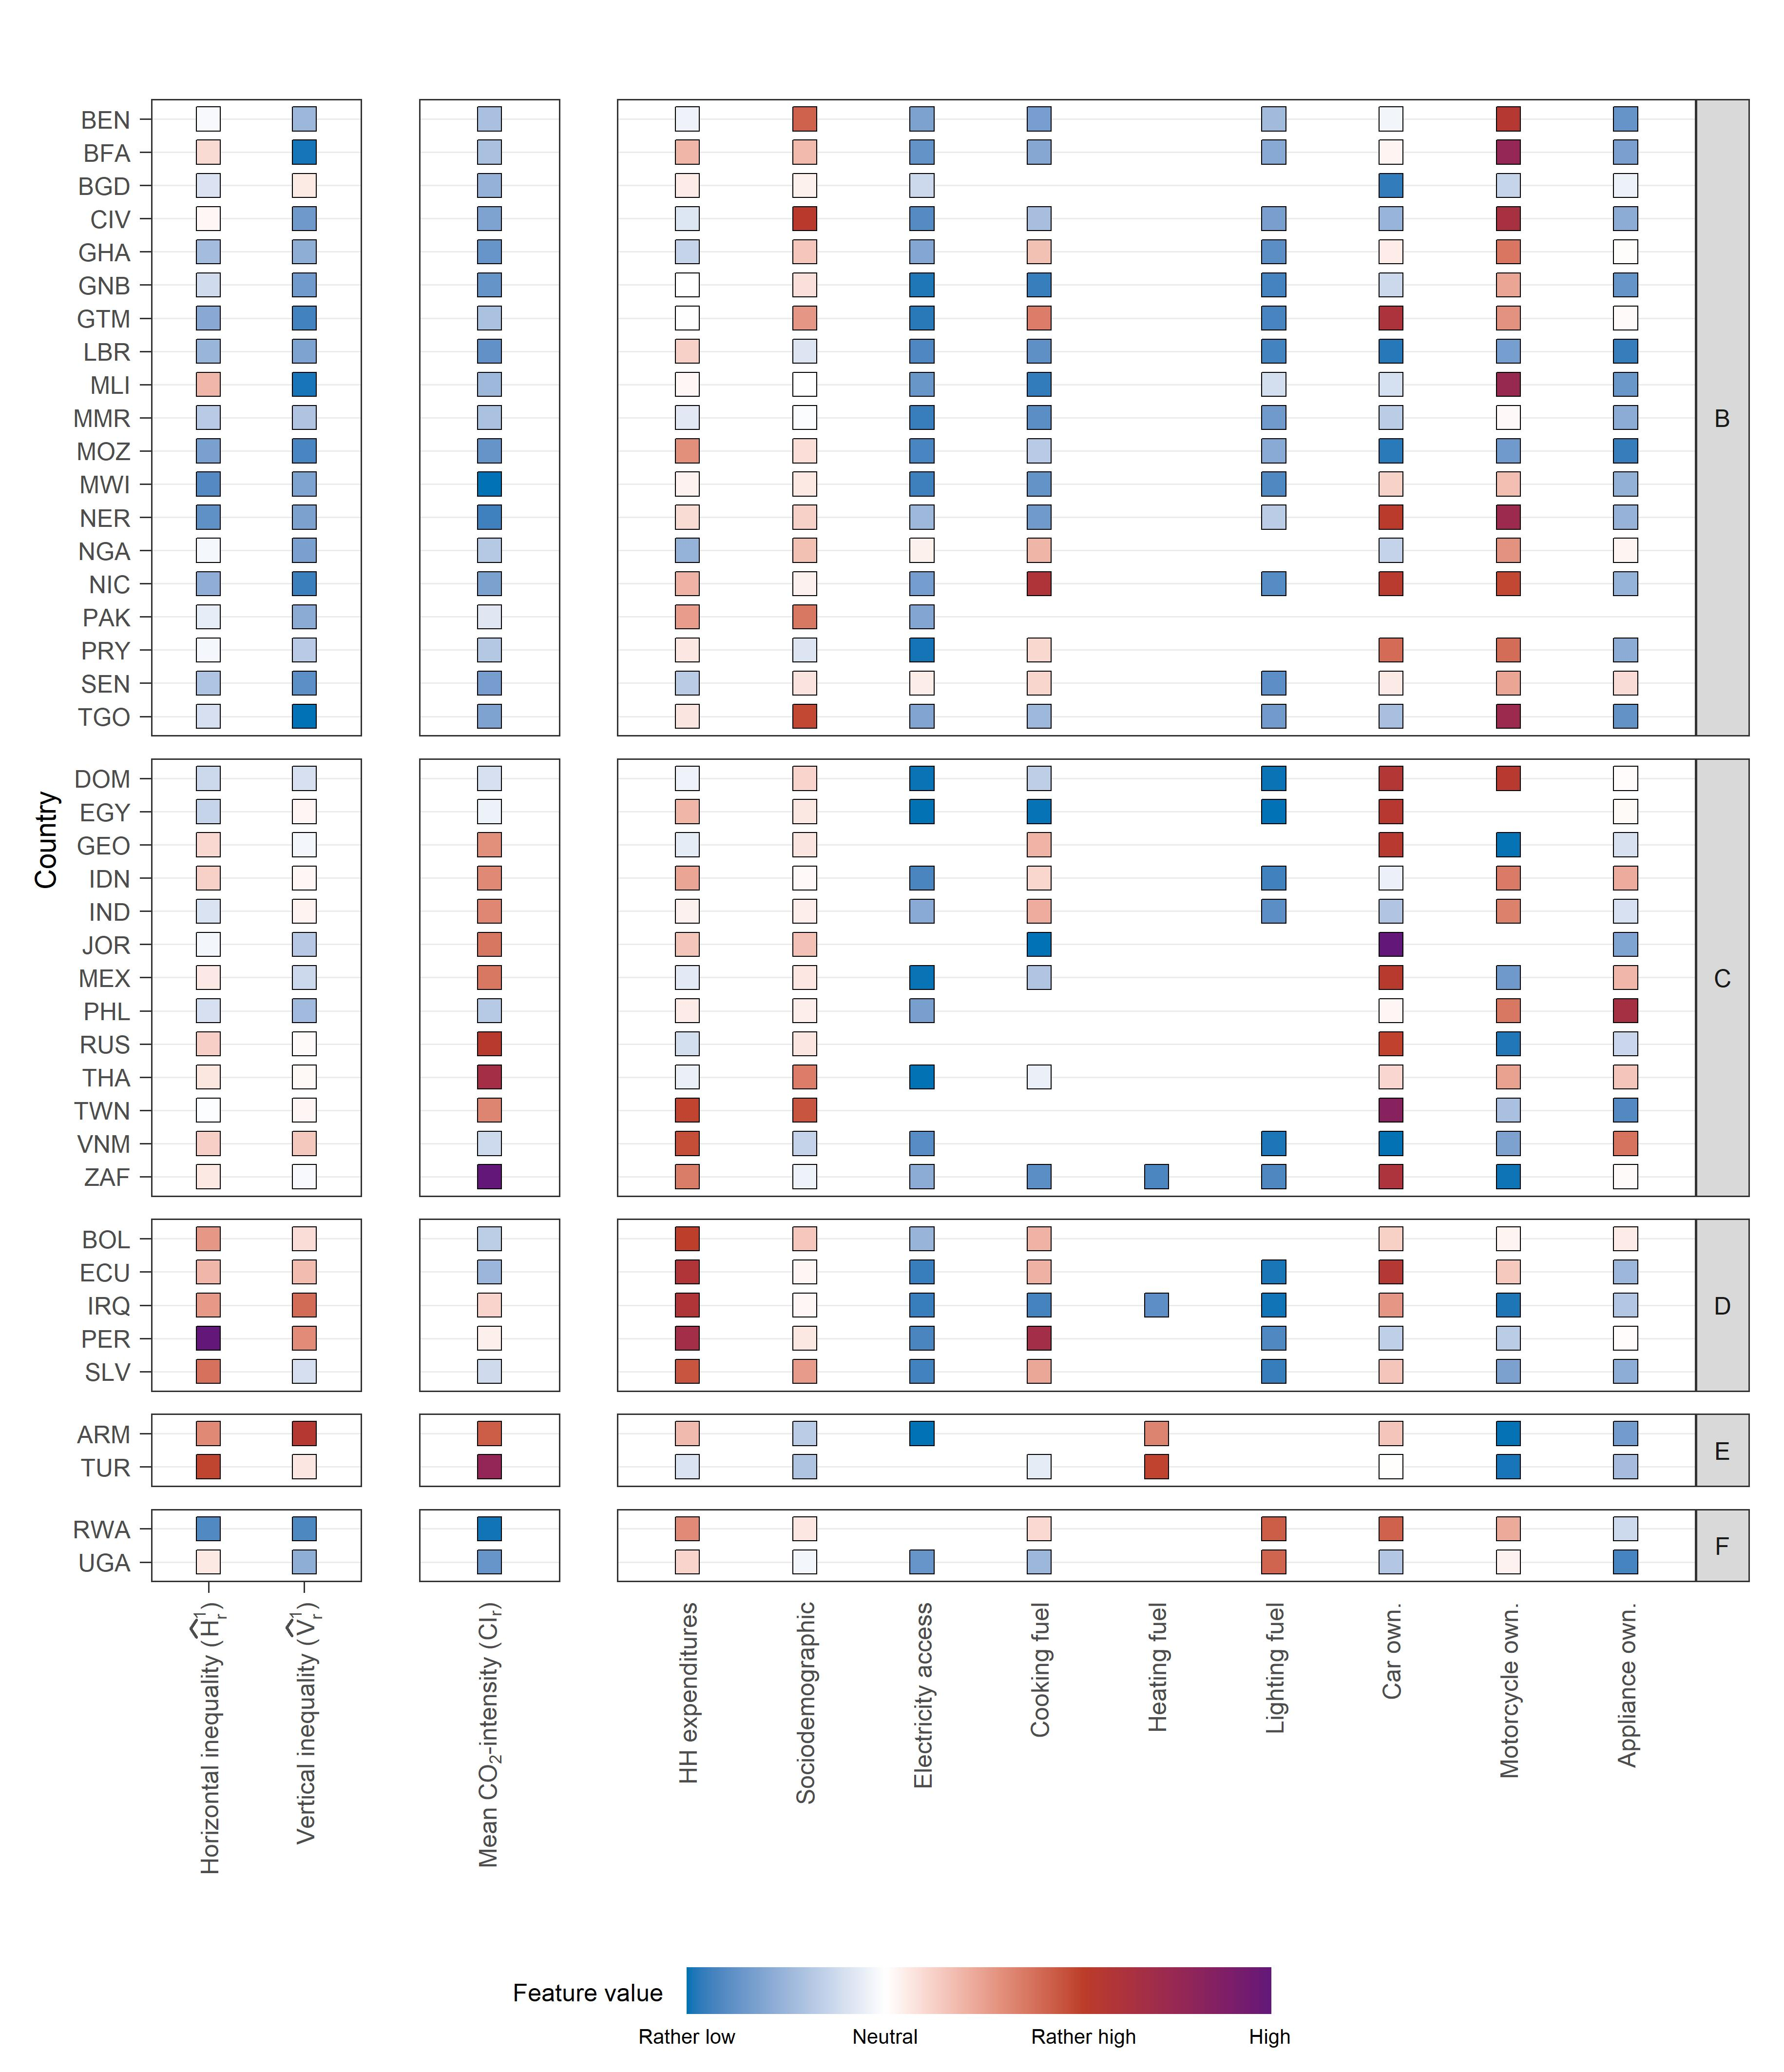
\includegraphics{Figure 4/Figure_4_Corrected_2}
    \caption{Feature importance across countries by cluster}
    \label{fig:fig_4_2}
    \begin{subcaption2}
    This figure shows the importance of features (in normalized average absolute SHAP-values) for each country, grouped by country clusters. Blue (red) colors indicate that a feature is relatively less (more) important in a country compared to all other countries. 'Sociodemographic' comprises normalized absolute SHAP-values for features such as ethnicity, nationality, religion or language.
    For horizontal inequality, blue (red) colors indicate a lower (higher) heterogeneity within the first income quintile compared to the fifth income quintile. For vertical inequality, blue (red) colors indicate lower (higher) median carbon intensity among the first income quintile compared to the fifth income quintile. For average CO$_{2}$-intensity, blue (red) colors indicate a lower (higher) average carbon intensity across all countries.
    We assign countries to 9 clusters performing k-means clustering based on scaled values across all features. We also show all values in Table \ref{tab:A10}.
    \end{subcaption2}
\end{figure}

%What are important criteria to assign countries to different clusters?

\begin{itemize}
    \item Discuss meaningful variables. Go on level of clusters to discuss direction and intuition of effects.
    \item Discuss country clusters in general and data issues, idiosyncracy. For each country cluster, one could recommend specific policy actions --> going to discussion section
\end{itemize}

\paragraph{Identifying country clusters}

We identify nine country-clusters based on feature importance for prediction of household-level carbon intensity, the average carbon intensity of households and the vertical and horizontal distribution of countries. Countries within clusters are more similar to each compared to countries in other clusters. In general, it is difficult to assign countries to clusters, as demonstrated through the optimal number of clusters ($k=9$) and an average silhouette width of 0.17 (see Figures \ref{fig:G3_silhouette_2} and \ref{fig:G4_silhouette_2}). This points to idiosyncratic patterns in some countries, which make it more difficult to draw conclusions for climate and compensation policies from the experience of other countries. 

Figure \ref{fig:fig_3} shows the relative importance of different features across country-clusters, while clusters are ordered by cluster size. Figures \ref{fig:5b_EST} to \ref{fig:5b_ARM} show variable importance plots and partial dependence plots with SHAP-values for those countries with highest silhouette width per cluster.

The largest cluster A comprises 36 countries (including \hyperref[fig:5b_USA]{USA}, \hyperref[fig:5b_CAN]{Canada}, \hyperref[fig:5b_BRA]{Brazil} or \hyperref[fig:5b_DEU]{Germany}). In countries of this cluster, our analysis yields more carbon-intensive consumption among relatively poorer households and a larger heterogeneity in carbon intensity among poorer households compared to richer households. In comparison to other clusters, most features contribute relatively little to explaining variation in carbon intensity. For example, average adjusted feature importance is 3\% for household expenditures, which is the most important feature across all countries. In general, countries in cluster A have in common that it is difficult to predict carbon intensity of households with available data. One reason is that we adjust country-level feature importance for models' predictive performance, which influences the identification of country clusters. For example, 17 out of 18 countries with relatively low model performance ($R^{2}<$10\%) appear in cluster A. In particular, data resolution may be insufficient and does not cover important variables (25 countries lack information on major cooking fuels, 21 countries lack information on car ownership). These results also allude to highly idiosyncratic characteristics of heterogeneous carbon intensity with important implications for policy design, because attempts to compensate based on characteristics observable in our dataset (such as household expenditures) will not be effective to compensate the households most affected by climate policy, but impacts can be large, as indicated by - on average - more carbon-intensive consumption (0.72 kgCO$_{2}$/US-\$ on average) compared to countries in other clusters. 

In contrast, cluster B includes 16 countries (such as \hyperref[fig:5b_IND]{India}, \hyperref[fig:5b_BGD]{Bangladesh} or \hyperref[fig:5b_KEN]{Kenya}) with less carbon-intensive consumption (0.33 kgCO$_{2}$/US-\$ on average). Within such countries, consumption is more carbon-intensive among richer households and we also find a larger heterogeneity among richer households compared to poorer households. In this cluster, vehicle ownership, cooking fuel use and appliance ownership are relatively more important compared to other clusters, while adjusted feature importance for household expenditures is 3.4\%, on average.

Cluster C comprises ten countries (such as \hyperref[fig:5b_IDN]{Indonesia}, \hyperref[fig:5b_MEX]{Mexico} and \hyperref[fig:5b_ZAF]{South Africa}) with comparably high average carbon intensity (1.04 kgCO$_{2}$/US-\$ on average). Within countries, differences in carbon-intensity are comparably small between poorer and richer households, but richer households consume more carbon-intensively in all countries but Vietnam. Countries have in common that household province, appliance and car ownership are important features.

Distinguishing between urban and rural households is an important feature in cluster D. In countries in cluster E, household expenditures and main cooking fuels are important predictors for carbon intensity. Compared to others, countries in cluster F stand out because of high adjusted feature importance for motorcycle ownership and sociodemographic variables. Households' main lighting fuel and province are relatively important features in countries of cluster G, while clusters H and I comprise relatively more carbon-intensive countries, in which household expenditures and car ownership (cluster H) and the main heating fuel (cluster I) are comparably relevant.

While being stylized by nature our clustering approach helps to emphasize country-specific characteristics correlating with (and contributing to) heterogeneous impacts of climate policy on households. Importantly, we provide evidence for differences in household expenditures (or income) being less decisive for households' carbon intensity than often suggested. Features describing households' energy use can be helpful predictors in some countries (for example of clusters B, E, F and H), but not necessarily in every context.     

\begin{figure}[ht!]
    \centering
    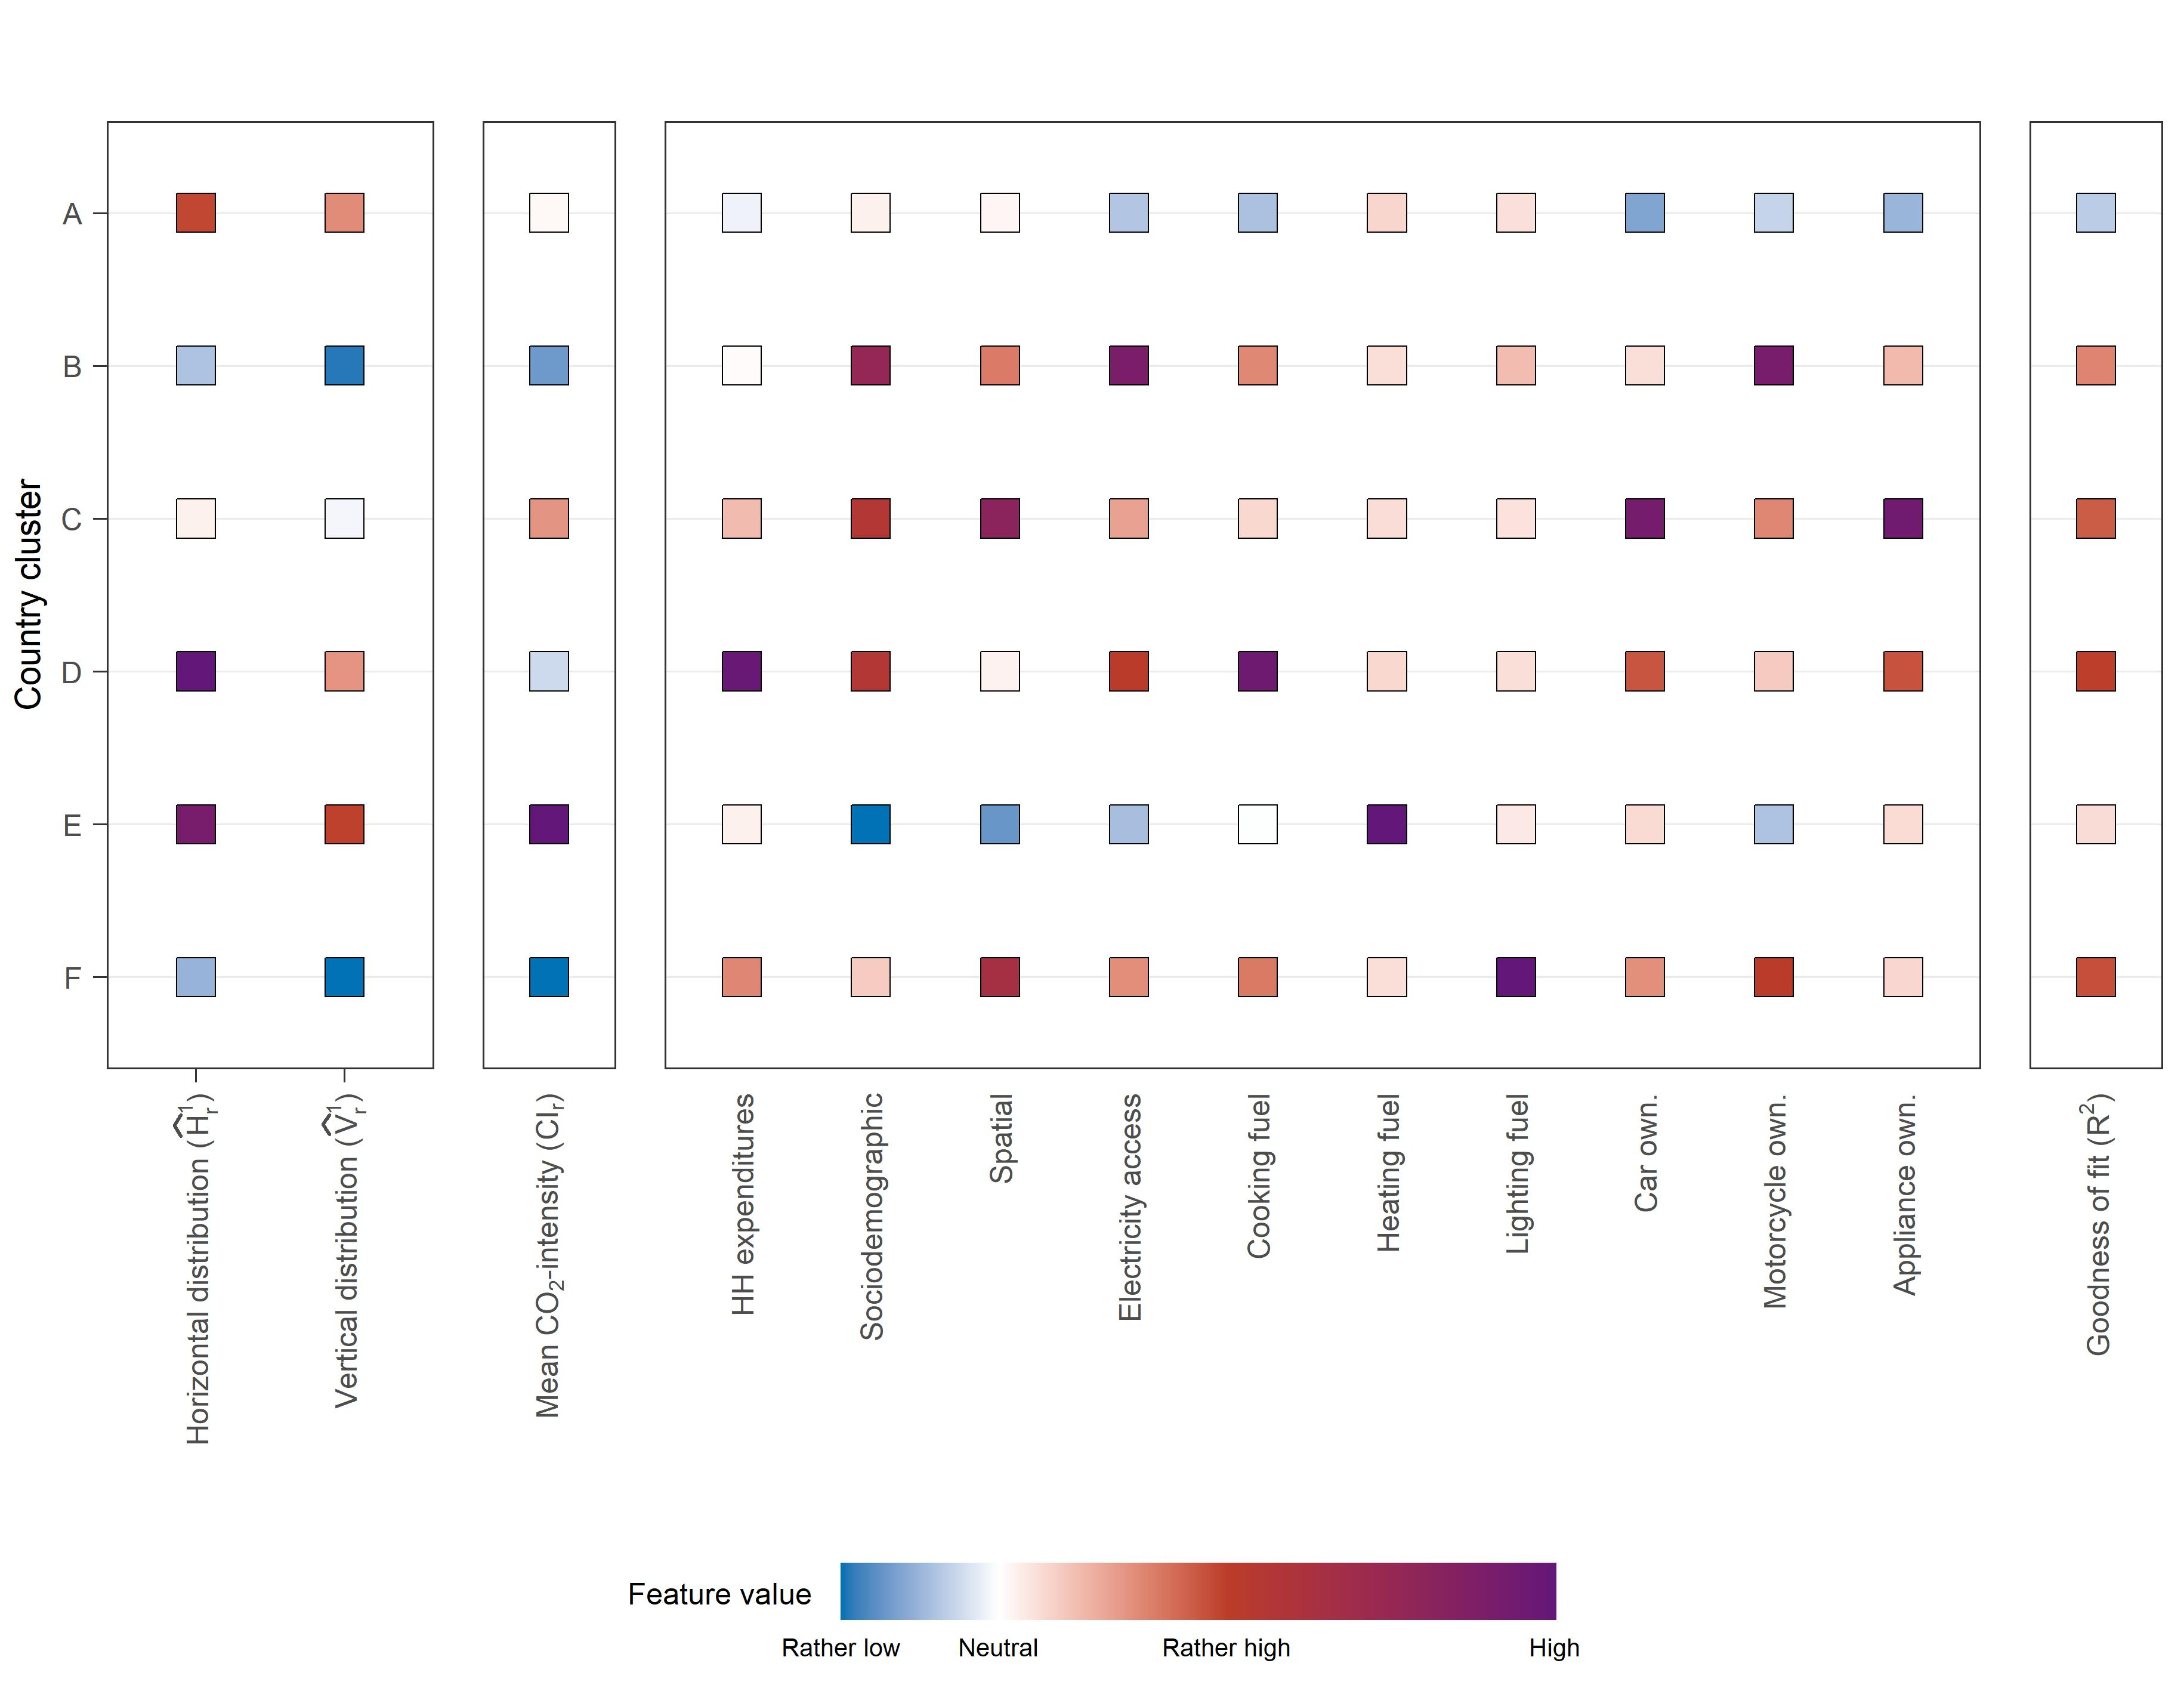
\includegraphics{1_Figures/Figure 3/Figure_3_Corrected.jpg}
    \caption{Average feature importance across country clusters}
    \label{fig:fig_3}
    \begin{subcaption2}
    This figure shows the average importance of features (in normalized absolute average SHAP-values) across all countries from each cluster A to I. Colors express the average importance of features in a cluster in comparison to other clusters. Blue (red) colors indicate that a feature is relatively less (more) important on average in a cluster compared to all other clusters. 'Sociodemographic' comprises normalized absolute average SHAP values for features such as ethnicity, nationality, religion or language.
    For horizontal inequality, blue (red) colors indicate a lower (higher) heterogeneity within the first income quintile compared to the fifth income quintile. For vertical inequality, blue (red) colors indicate lower (higher) median carbon intensity among the first income quintile compared to the fifth income quintile. For average CO$_{2}$-intensity, blue (red) colors indicate a lower (higher) average carbon intensity across clusters. We assign countries to 14 clusters performing k-means clustering. We also show all values in Table \ref{tab:A9}.
    \end{subcaption2}
\end{figure}

\paragraph{Household characteristics and heterogeneous carbon intensity of consumption}

Partial dependence plots (Figures \ref{fig:5b_EST} to \ref{fig:5b_ARM}) show SHAP-values for different feature values. 

Supplementary analyses building on a logit-model corroborate these findings


% \begin{figure}[ht!]
%     \centering
%     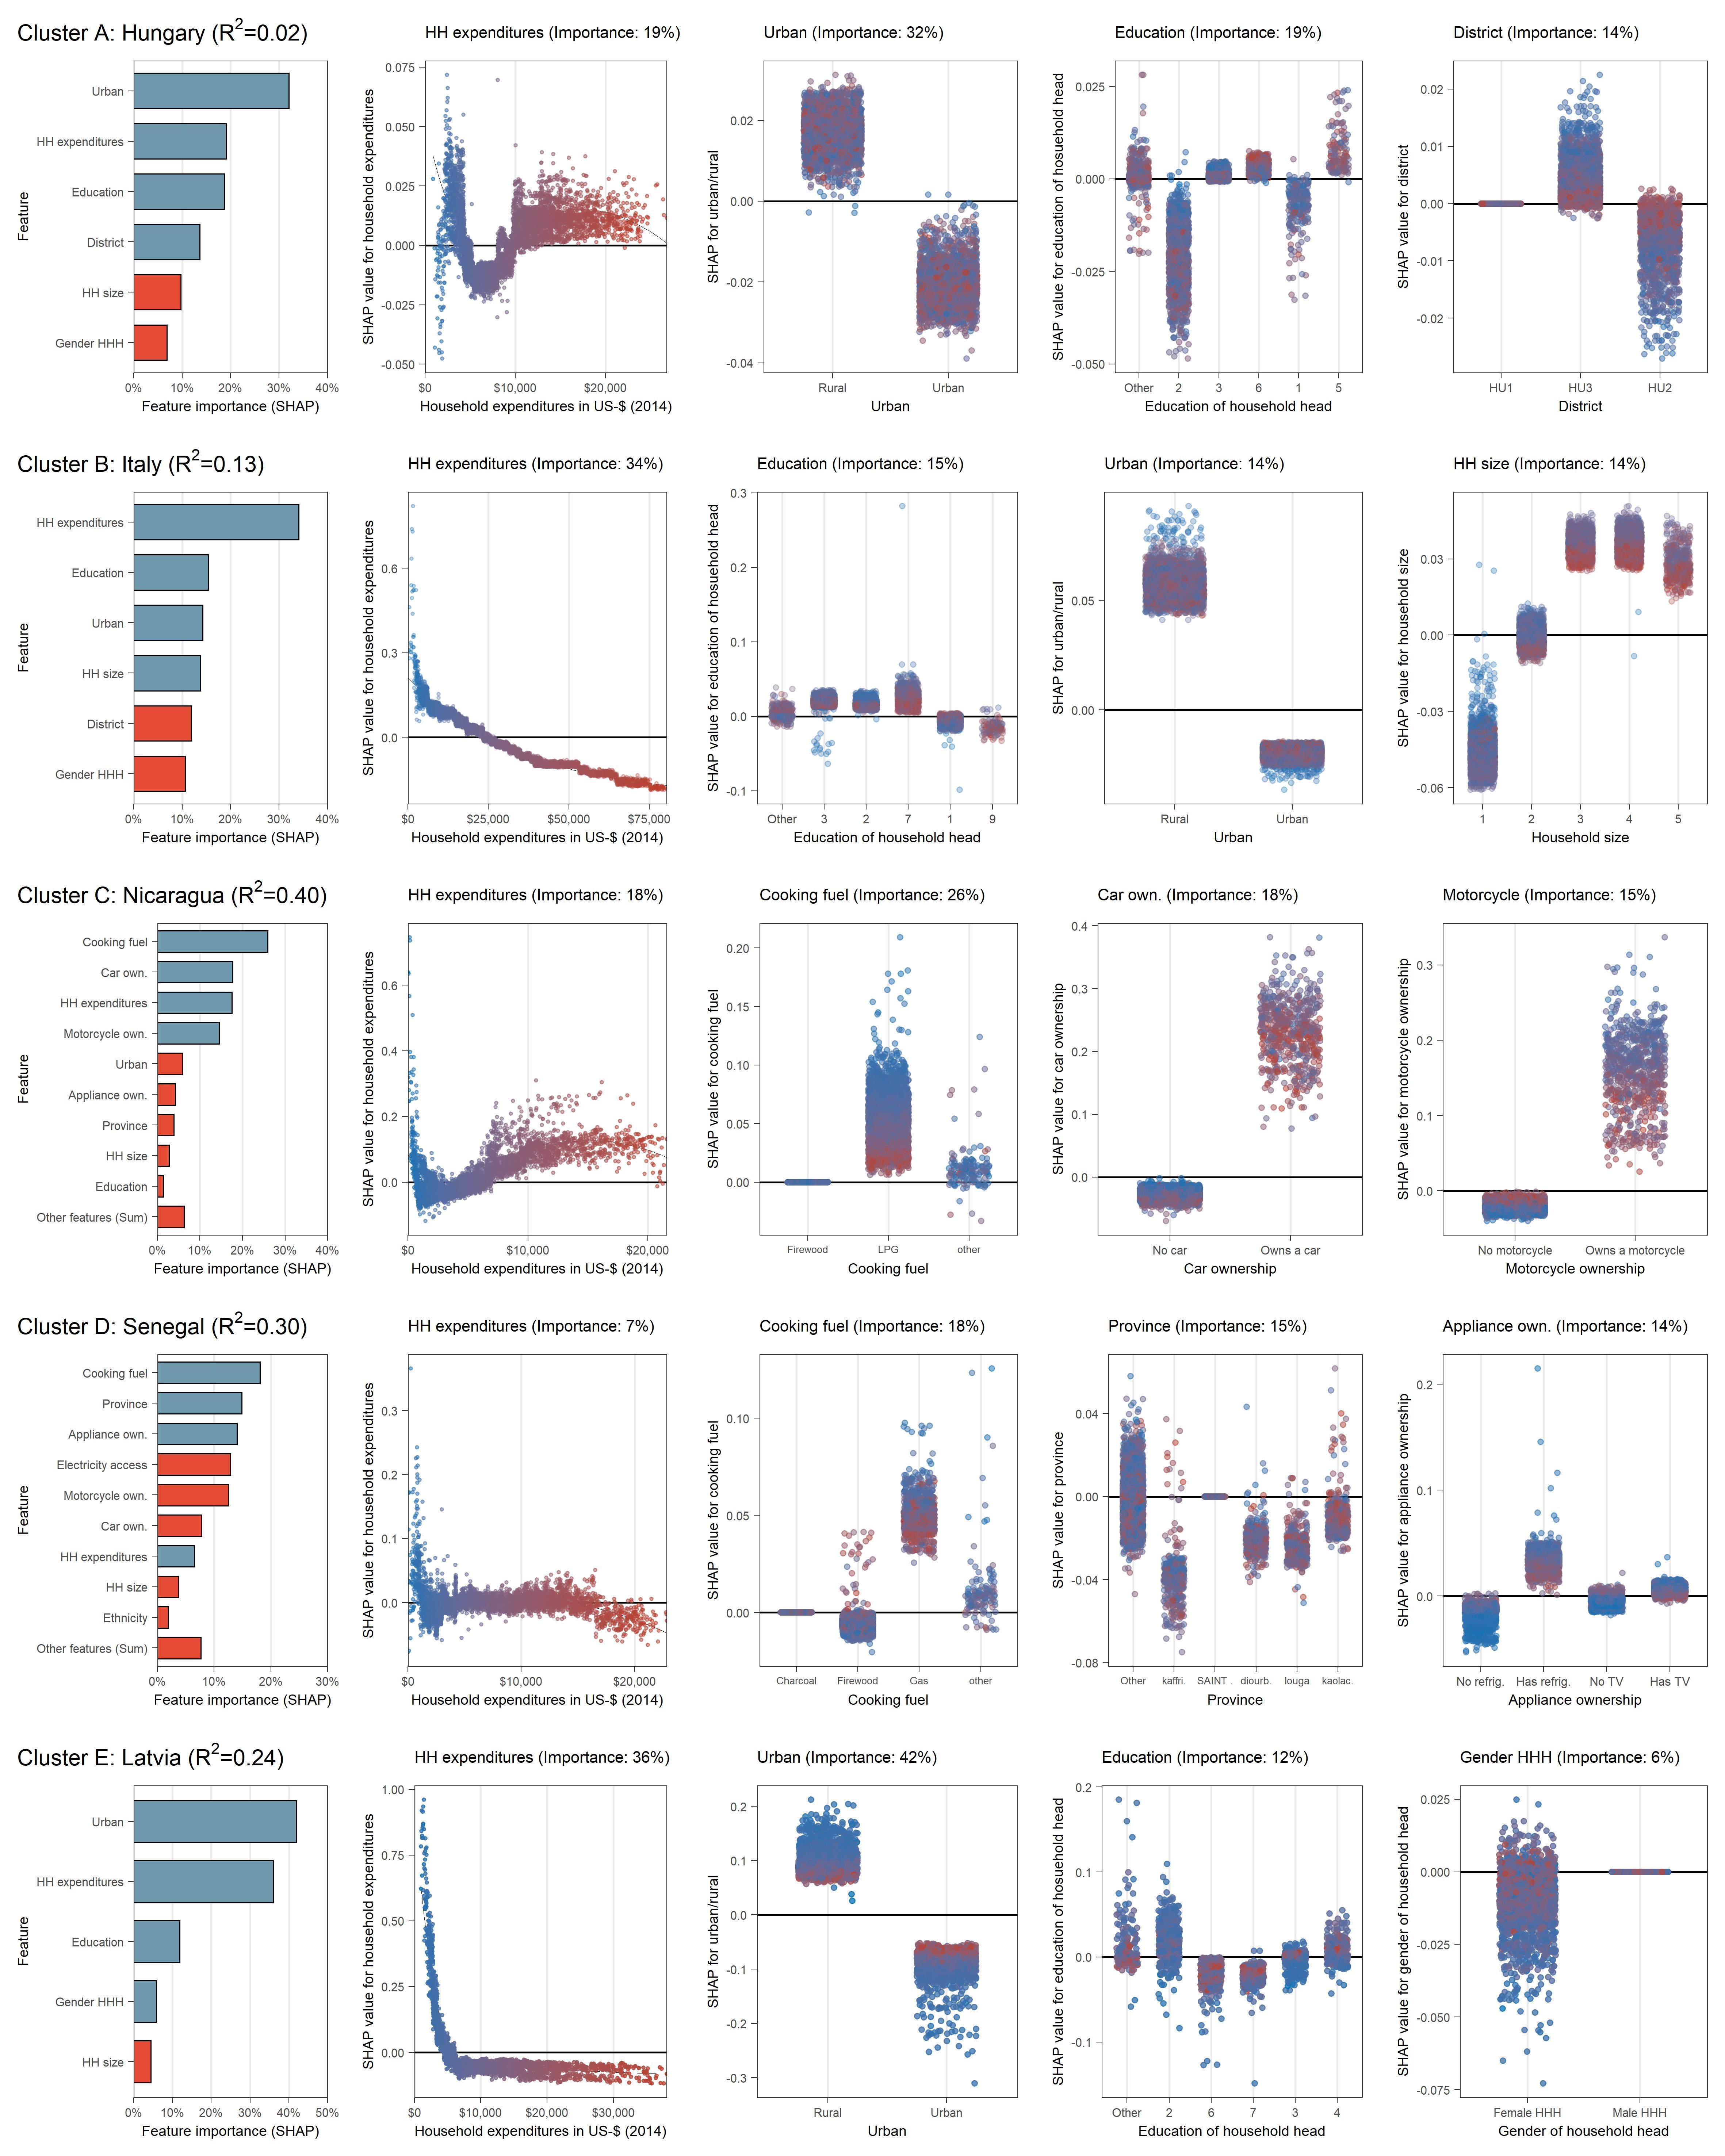
\includegraphics[width=15.5 cm]{Figure 5/Figures_joint_1}
%     \caption{Partial dependence plots (SHAP) for one country in clusters A to C}
%     \label{fig:fig_5_1}
%     \begin{subcaption2}
%     This figure shows SHAP-values for predicting carbon intensity over feature values for one representative country in each country-cluster in rows. The bar chart displays normalized average absolute SHAP-values for all features. Features with less than 3\% of normalized SHAP-values are subsumed as "Other features (Sum)". Charts show SHAP-values over total household expenditures for all countries and for the three most important features in each country besides total household expenditures. Colors represent household expenditures with blue (red) colors indicating lower (higher) household expenditures. See also Appendix REF to REF.
%     \end{subcaption2}
% \end{figure}

% \begin{figure}[ht!]
%     \centering
%     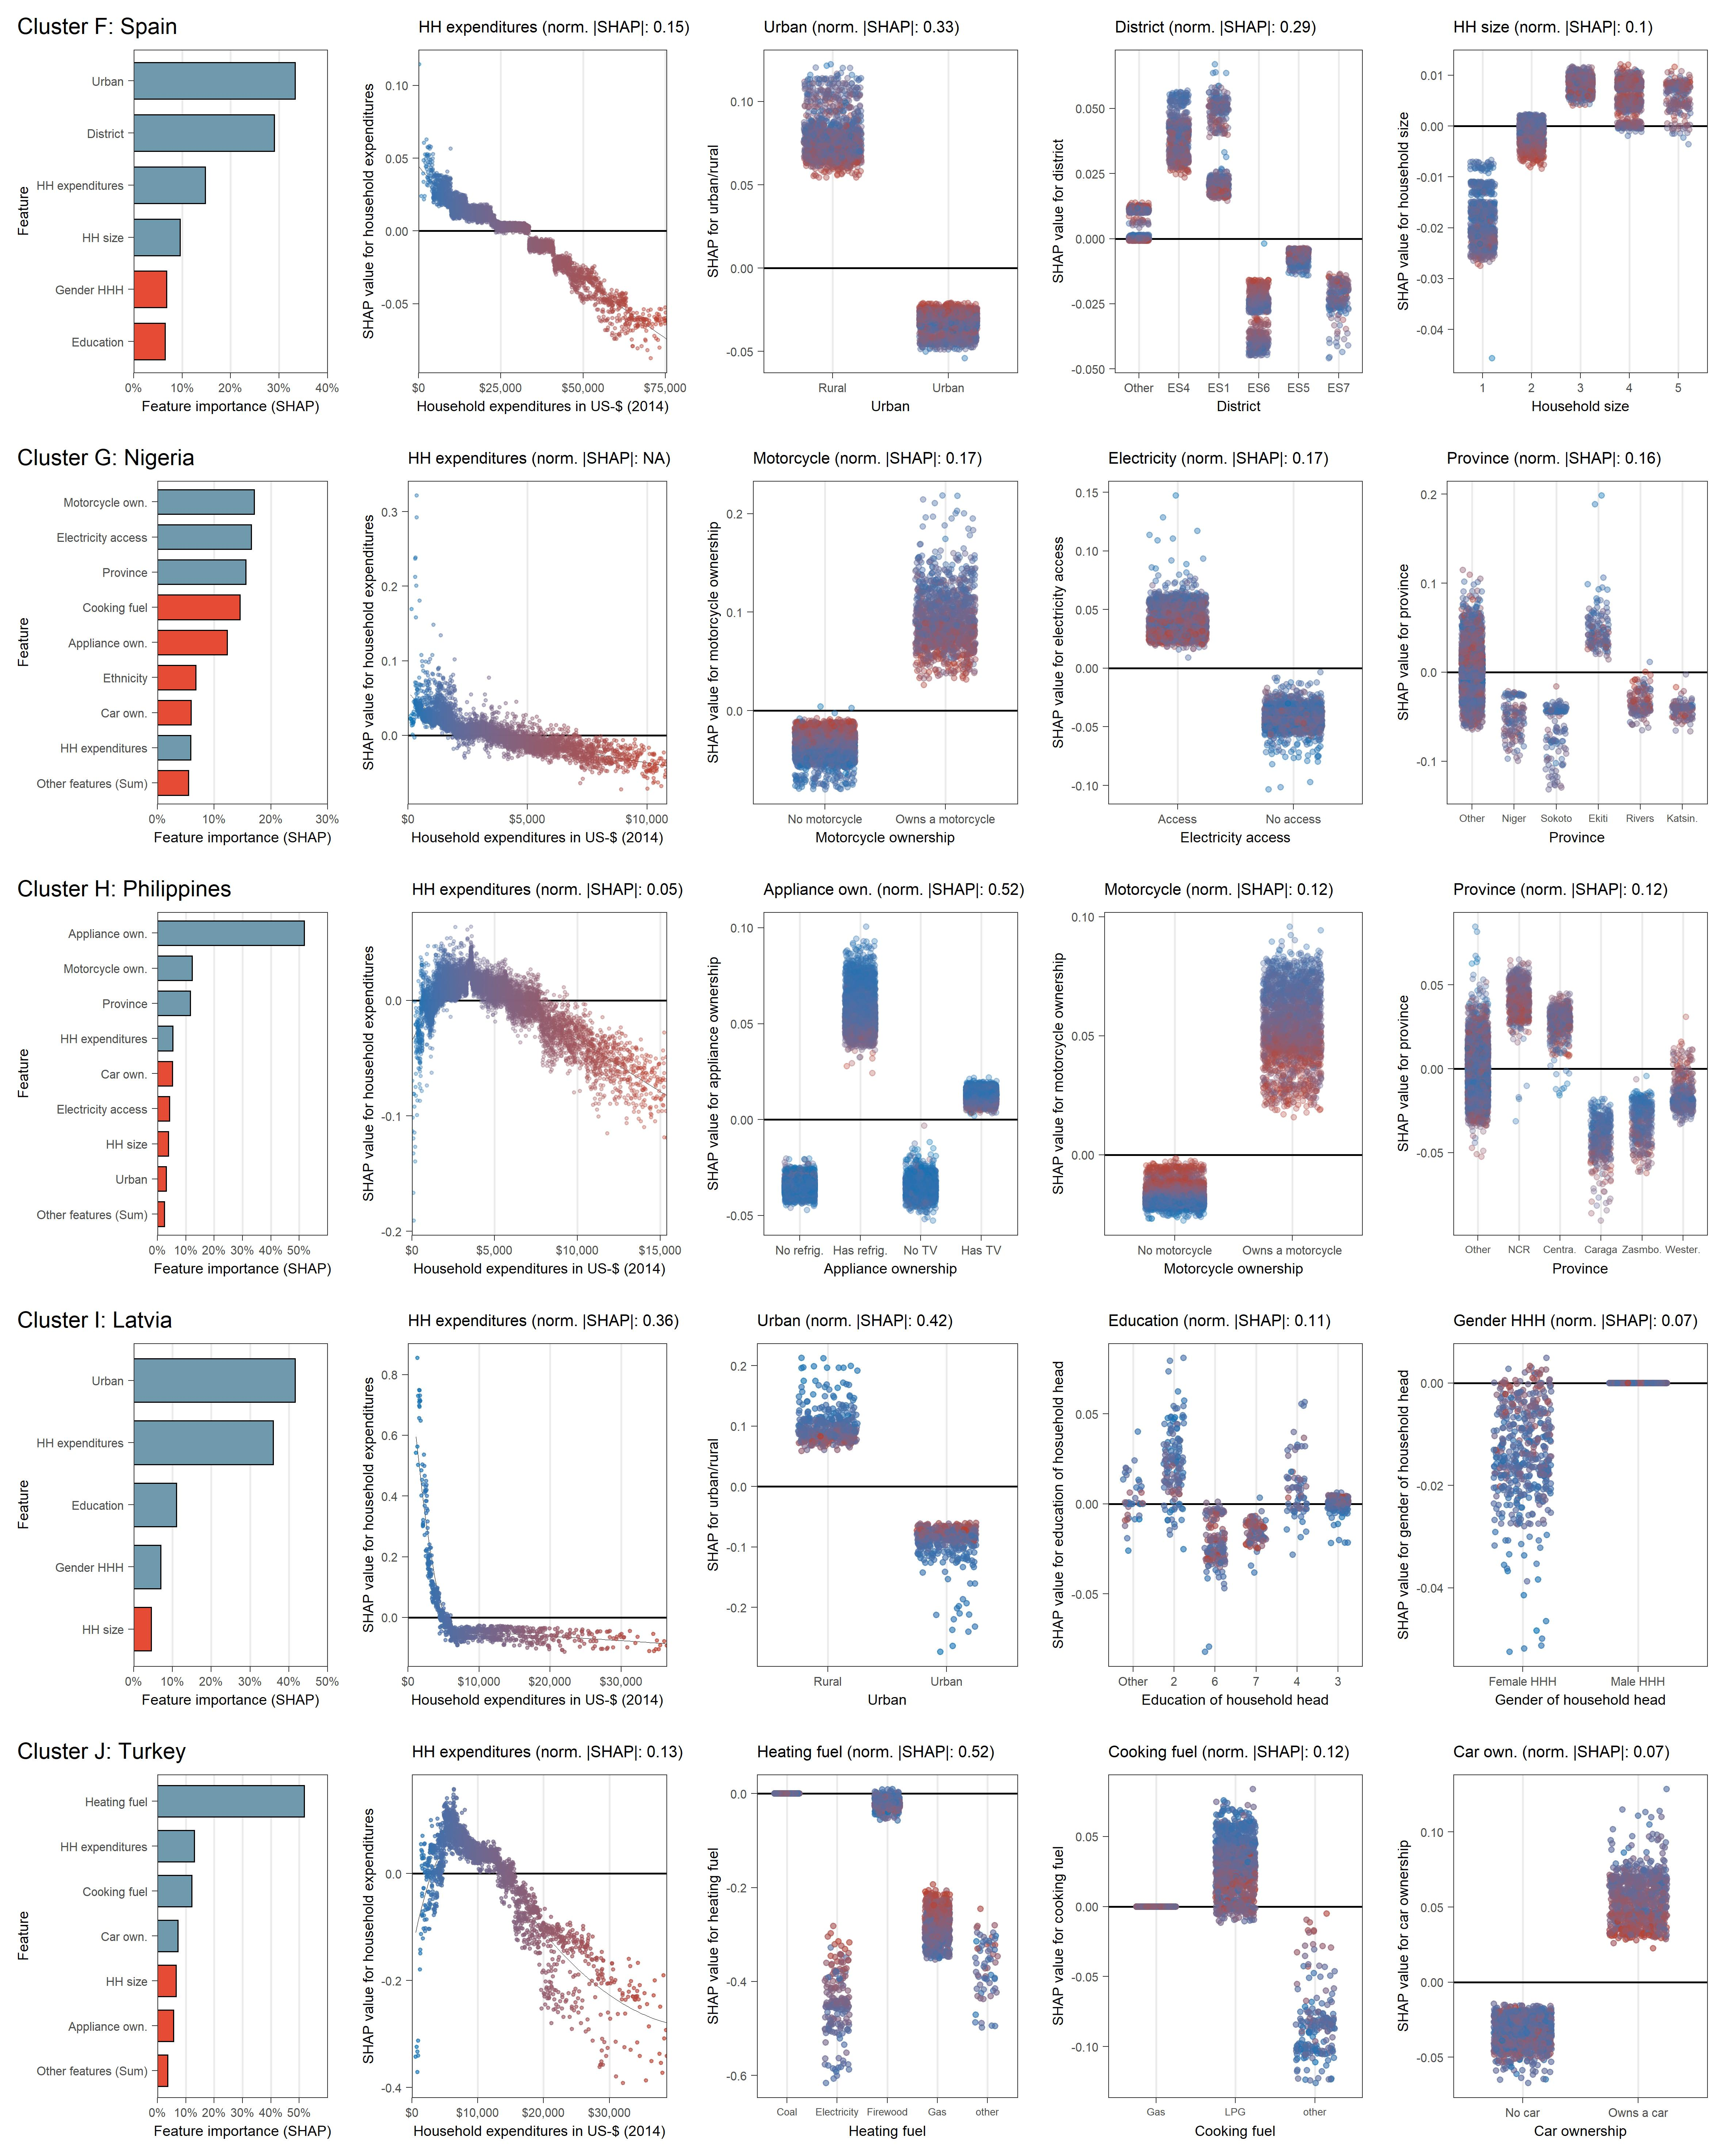
\includegraphics[width=15.5 cm]{Figure 5/Figures_joint_2}
%     \caption{Partial dependence plots (SHAP) for one country in clusters D to F}
%     \label{fig:fig_5_2}
%     \begin{subcaption2}
%     This figure shows SHAP-values for predicting carbon intensity over feature values for one representative country in each country-cluster in rows. The bar chart displays normalized average absolute SHAP-values for all features. Features with less than 3\% of normalized SHAP-values are subsumed as "Other features (Sum)". Charts show SHAP-values over total household expenditures for all countries and for the three most important features in each country besides total household expenditures. Colors represent household expenditures with blue (red) colors indicating lower (higher) household expenditures. See also Appendix REF to REF.
%     \end{subcaption2}
% \end{figure}

% \begin{figure}[ht!]
%     \centering
%     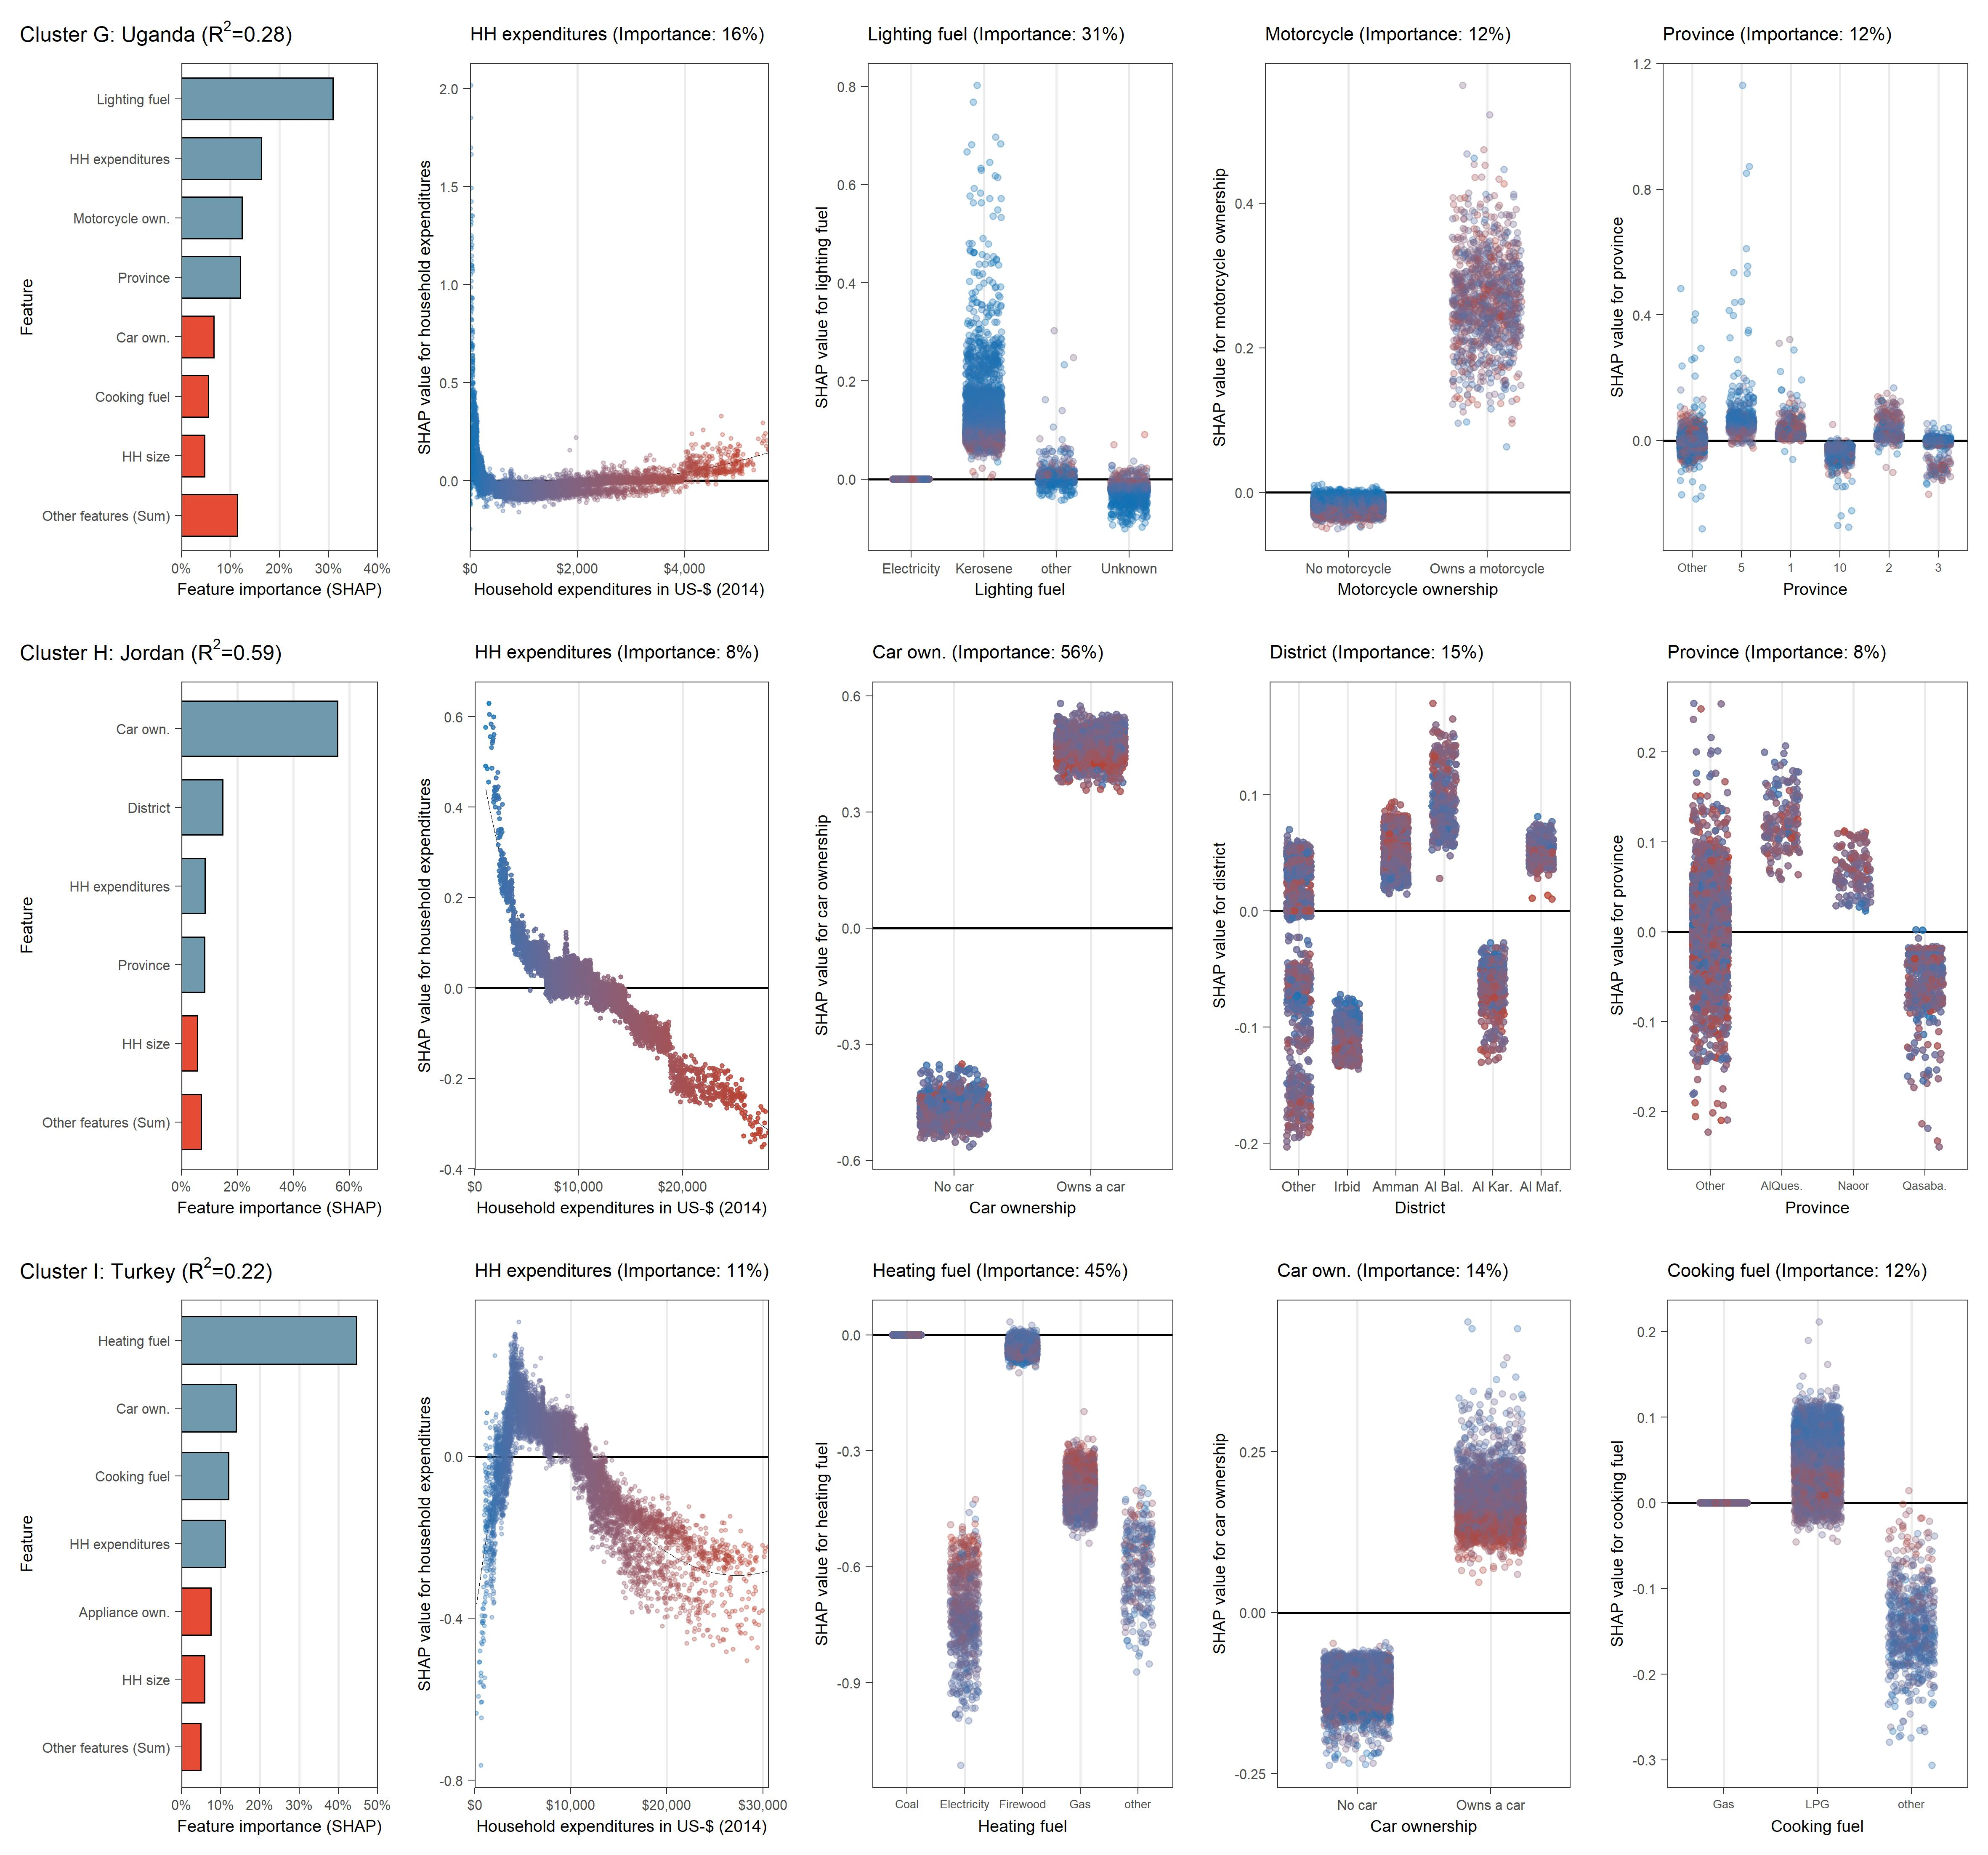
\includegraphics[width=15.5 cm]{Figure 5/Figures_joint_3}
%     \caption{Partial dependence plots (SHAP) for one country in clusters G to I}
%     \label{fig:fig_5_3}
%     \begin{subcaption2}
%     This figure shows SHAP-values for predicting carbon intensity over feature values for one representative country in each country-cluster in rows. The bar chart displays normalized average absolute SHAP-values for all features. Features with less than 3\% of normalized SHAP-values are subsumed as "Other features (Sum)". Charts show SHAP-values over total household expenditures for all countries and for the three most important features in each country besides total household expenditures. Colors represent household expenditures with blue (red) colors indicating lower (higher) household expenditures. See also Appendix REF to REF.
%     \end{subcaption2}
% \end{figure}

\begin{itemize}
    %\item (Tendenziell ginge auch out-of-sample prediction mit detaillierter Auflösung, wie einzelne features (SHAP) zur gesamten Prediction beitragen).
    \item Marginal effects of logit-models per country for easier visualization. Across countries to Appendix.
    %\item Summary statistics
    %\item Show differences between poor and rich households.
    %\item Show differences within poor and rich households.
    %\item One figure: One country (quintiles and boxplots), all countries (poorest quintile and between-quintile differences), all countries (vertical over horizontal inequality)
    %\item Within-quintile differences exceed between-quintile differences
    %\item Horizontal heterogeneity even more pronounced than vertical heterogeneity in majority of countries
    %\item Households that consume more carbon-intensively than others are poorer than others in richer countries and richer than others in poorer countries. Explain basic intuition.
    %\item If within-quintile differences exceed between-quintile differences using differences in income as a main indicator for evaluating heterogeneity is insufficient.
    %\item Learning about the most carbon-intensively consuming households and their characteristics (beyond income) is important.
    %\item Discuss main arguments for single characteristics (possibly already in methods section).
    \item Show results for different characteristics.
    %\item One figure: One country (Marginal effects from Logit-model), Shapley-values from boosted regression trees
    %\item One figure: Comparing marginal effects from Logit-model across countries
  \item Robustness checks from Logit in text, but figures or tables to Appendix. More carbon-intensive households are more likely to own (and use) a car, more likely to use fossil fuels for cooking, such as coal, gas, or LPG, less likely to use firewood, charcoal or biomass for cooking, compared to households cooking with electricity. More likely connected to the electricity grid, more likely to have secondary or higher education, more likely to live in rural areas (in richer countries). Discuss differences in space, across provinces and districts. Depending on the country-context, they are more/less likely to identify with ethnic majorities or minorities.
   %\item Comparing model outcomes across countries. One figure: A: Show classification for single countries with colour codes (order in clusters). B: Show clustering of countries with colour codes.
  % \item Discuss differences in instruments: electricity sector instruments, transport sector instruments, international trade policy etc. Highlight main differences: electricity sector characteristics and electrification critical for electricity sector instruments, transport sector policies likely regressive in richer countries, progressive in poorer countries, carbon border adjustments more likely to affect people who consume more carbon-intensive and imported goods and services. Non-consumption impacts probably more severe. (If anything, possibly also Appendix. I suggest the figure comparing vertical and horizontal aspects here - in Appendix).
\end{itemize}

\paragraph{Heterogeneous impacts of sectoral and regional policies}

Our flexible analytical framework also allows for investigating the heterogeneous impacts of different policies by including or excluding CO$_{2}$-emissions from different sectors or regions. For example, Figure \ref{fig:comparison_policies} compares vertical and horizontal distribution coefficients for a national climate policy (as in Figure \ref{fig:fig_2}) and international climate policy, i.e. price increases in equivalence to embedded \textit{global} CO$_{2}$-emissions, and to policy instruments that increase consumer prices in equivalence to embedded national CO$_{2}$-emissions from the transport and electricity sector, respectively.  The comparison of vertical and horizontal inequality across policies emphasizes policy-specific differences within expenditure quintiles: In comparison to national climate policy, international climate policy would lead to more heterogeneous impacts in richer households in 23 countries, because richer households usually spend relatively more on imported goods and services. For transport sector policies, we document more carbon-intensive consumption among richer households compared to poorer households in 59 countries while horizontal differences exceed vertical differences in 77 countries. In contrary, our findings indicate that electricity sector policies would likely more heavily affect poorer households in 62 countries with larger horizontal heterogeneity among poorer households in 64 countries\footnote{Both findings are in contrast to national climate policy across all sectors: We find more carbon-intensive consumption among richer households in richer households compared to poorer households in 43 countries. Within-quintile heterogeneity is larger among poorer households in 58 countries and horizontal inequality exceeds vertical inequality in 66 countries.}. 
On aggregate, these results underpin that distributional implications of climate policy are country- and policy-specific, but that within-quintile heterogeneity is meaningful, hinting to limited leeway for effective cross-country policy learning.

%\begin{itemize}
%\item Vertical and horizontal indicators: In how many countries?
% \item National 43 regressive, 44 progressive - 58 larger among poorer households - horizontal exceed vertical in 66 countries
% \item Global 45 regressive, 42 progressive - 54 larger among poorer households - horizontal exceed vertical in 58 countries. Story here is that inequality among richer households increases because richer households have a larger taste for imported goods and services.
% \item Transport 28 regressive, 59 progressive - 49 larger among poorer households - horizontal exceed vertical in 77 countries. Story here is very progressive results with large horizontal inequality!
%\item Electricity 62 regressive, 25 progressive - 64 larger among poorer households - horizontal exceed vertical in 62 countries. Story here is more regressive results with large horizontal inequality among poorer households.
% \end{itemize}

\section{Discussion: XYZ} \label{sec:discussion}

\begin{itemize}
\item Our findings provide evidence for country-specific characteristics associated to higher levels of carbon intensity of consumption. These results can help in ex-ante assessments to identify especially affected household profiles and promising means to compensate them. Building on identified clusters, we discuss implications for potential compensation.
  \item Discuss role of findings for design of transfers. What is being discussed? LST, tax breaks, infrastructure access. Which transfer tool is applicable in which context?
  \item Very important: Low predictive power means that any transfer will be ineffective to some extent! Important concern.
  \item Discuss normative or theoretical grounds for either transfer option or the other.
\item Discuss ``value chain of climate policy implementation''. Discuss literature on public acceptance. Highlight research gaps: Which distributional implications matter to households and why? How could compensation increase public support? Public support of which groups matter for people with political power? Could be first starting point for discussion.
 \item Discuss role of findings for design of different policies (standards, subsidies, brief ?)
 \item Discuss dynamic effects and inaccuracies in modeling approach (tax pass-through, short- vs. medium-term, technological path dependencies/barriers on household-level)
 \item Distinguish results from analyses about climate policy on labour, wealth, impacts, adaptation, co-benefits, co-costs.
 \item Investments: Not covered, only consumption.
\end{itemize}

\section{Conclusion} \label{sec:conclusion}

\begin{itemize}
 \item Differences in income one important criterion for comparing outcomes across groups.
 \item Misses important parts of the picture. Necessary to factor in other characteristics.
 \item More nuanced analyses can help to facilitate discussion on acceptable climate policy.
\end{itemize}

\clearpage

\printbibliography

\clearpage

\appendix 
{\Huge Appendix} \label{sec:appendix}

Global heterogeneity in carbon intensity of consumption

\clearpage
\section{Data cleaning} \label{sec:cleaning}

We describe our approach to collecting, cleaning and homogenizing microdata and to feature engineering for machine learning modeling.

\subsection{Collecting household data}

We collect household budget survey data and extract several information before cleaning and homogenizing. Household budget survey data are often publicly available, but sometimes subject to a considerable fee. Table X provides publishing organizations, names of surveys and links to datasets used in this study.

\begin{itemize}
    \item For each household, we include sociodemographic information about household members where available. In all survey, households are represented through 'household heads', i.e., persons who often contribute the largest share of household income or are responsible for purchase decisions. We use information for the 'household head' as a proxy for the entire household and collect information on education, occupation, gender, self-identified ethnicity, nationality or religion of the 'household head'. We standardize information on education by using the International Standard Classification of Education (ISCED) to facilitate comparison across countries.
    \item We include spatial information where available, for example identifier for sub-national areas (provinces), sub-sub-national areas (districts) or villages. Often, surveys include an indicator for whether households live in urban or rural areas. Definitions of \textit{urban} and \textit{rural} may not be consistent across countries, but within countries.
    \item We include information on energy use, such as on primary fuels used for cooking, lighting and heating. We homogenize information on fuels across countries to account for different names and levels of detail across countries. For example, cooking fuels include charcoal, coal, electricity, firewood, gas, kerosene, liquid fuel, LPG, other biomass or unknown fuels.
    \item We capture information on electricity access and create a binary variable indicating if households have access to electricity through electricity grids, but also through generators or solar panels. 
    \item We collect information about ownership of major transport vehicles (such as cars, motorcycles and trucks) and major household appliances (such as refrigerators, air conditioning, washing machines and television). For each country, we only include information about ownership, not about the precise number of owned vehicles and appliances to improve consistency across countries.
    \item We collect all available information on household-level expenditures, integrating information from household-level and individual-level diary entries. We do not include consumption information from home production, received as gifts or as remuneration for labor. Our rationale is that it would be difficult to cover self-produced goods and services that are not purchased on markets. We include all expenditures on the item-level and extrapolate expenditures to yearly values. Often, households track expenditures over the course of a few weeks, but provide details on less frequent purchases in the past months or year. This approach neglects seasonal consumption patterns, but resulting bias should be sufficiently small, since households are surveyed throughout the year.
    \item We do not include imputed expenditures, e.g., for hypothetical rental payments, since including them would give an inaccurate representation of household consumption.
\end{itemize}

Code written for each country-level dataset can be found in a stable online repository (INSERT LINK).

\subsection{Cleaning and homogenizing household data}

Building on raw microdata from household budget surveys we perform several cleaning steps in order to homogenize datasets across countries.

\begin{itemize}
    \item We remove households with missing information for variables such as household size, sampling weights or total expenditures.
    \item We address outliers of household expenditures at the item-level. We consider any observation an outlier if it is in the 99$^{th}$ percentile of all non-zero expenditures. We replace this observation with item-level median expenditures.
    \item We remove observations if expenditures are negative, for example, if households sell items.
    \item We remove duplicates from our sample. We check separately for duplicates at the level of household-level information and at the level of item expenditures: We consider households spending the same amount of money on the same items duplicates.
    \item We remove all households from our sample if aggregate expenditures exceed mean expenditures by five standard deviations ($z>5$).
    \item We use inflation rates from \textcite{IMF.2020} and exchange rates from the \textcite{WorldBankGroup.2023} to convert all local currencies to US-\$ for the year 2017. Expenditures from surveys conducted before 2017 are inflated; expenditures from surveys after 2017 are deflated. This ensures consistency with calculated CO$_{2}$-emissions as they refer to the year 2017. This approach does however neglect that expenditure shares may change with rising incomes and inflation.
    \item We create matching tables to assign country-level expenditure items to 65 aggregate sectors and to four broad expenditure categories (energy, food, goods, services). Items, that are difficult to match to a specific sector or to a specific category, e.g., 'other expenses', are matched to artificial sectors and categories labeled 'other'. We delete observations for items indicating aggregate categories, if this would lead to double-counting of single expenditures. We delete observations for items indicating taxes, since including them would prove inaccurate to calculate expenditure shares and because items indicating tax payments are not available in each country. We also identify items indicating energy use and create separate columns listing expenditures for different energy items, such as electricity, gasoline, diesel, kerosene, LPG, natural gas, charcoal, hard coal, firewood and other biomass. All matching tables are available through a separate stable online repository (INSERT LINK).
    \item We macth items pertaining to fuels such as firewood, charcoal and other biomass to the sector \textit{lumber} to account for indirect emissions attributable to production, transportation and retail of these goods. However, we treat direct CO$_{2}$-emissions as zero, in line with assumptions by the IPCC (REF MISSING).
\end{itemize}

We homogenize information on household characteristics across countries, for example for main cooking fuels, lighting fuels and heating fuels. If available, we collect information on household-level appliance and vehicle ownership and electricity access. We also include information on sociodemographic characteristics (including gender of household head, education of household head, self-identified ethnicity, nationality, language or religion).
We assign household to expenditure quintiles based on total household expenditures per capita to account for differing expenditure shares in larger households. 

Tables \ref{tab:A1}, \ref{tab:A2}, \ref{tab:A3}, \ref{tab:A4_CF}, \ref{tab:A5_LF} and \ref{tab:A6} show summary statistics for our final homogenized dataset. 

% tracking and documenting removals

\subsection{Feature engineering} \label{sec:featureengineering}

Building on our homogenized dataset, we perform feature engineering on our variables (features) before performing analyses with BRT.

\begin{itemize}
    \item We exclude any feature with missing variation (for four countries).
    \item We exclude categorical feature with extremely high granularity (such as district-level identifiers).
    \item We exclude any feature with missing values.
    \item We remove the minimum number of features necessary to avoid high levels of correlation ($r>0.9$) between all features.
    \item We code observations as "other" for each feature (except province-level, district-level and urban-/rural-identifiers) that account for less than 5\% of all observations.
    \item All country-level feature sets include total household expenditures (in US-\$ 2017) and household size. The minimum number of included features is X (for Y) and the maximum number of included feature is X (for Z).
\end{itemize}

\subsection{Policy simulation}\label{sec:policysimulation}

We show that heterogeneity in household-level carbon intensity of consumption is equivalent to heterogeneity in household-level carbon pricing incidence, assuming that producers pass-on carbon prices to consumers and that the carbon pricing incidence reflects over-night costs to households without demand responses.

The carbon intensity of consumption $e_{i}$ consists of sectoral carbon intensities and household-level sectoral expenditure shares as shown in equation \ref{eq:ei}. 

Carbon pricing can be thought of a tax $\tau$ in USD/tCO$_{2}$ and the total absolute costs from carbon pricing equals direct and indirect carbon emissions embedded in household consumption $E_{i}$ multiplied with $\tau$. Computing total relative costs $CPI_{i}$ requires division by total household expenditures $C_{i}$:

\begin{equation}
    CPI_{i} = \frac{E_{i}*\tau}{C_{i}}
\end{equation}

Relative additional costs, i.e., the carbon pricing incidence CPI$_{i}$ can be expressed in \% ($\frac{USD_{\tau}}{USD_{i}}$). CPI$_{i}$ is equivalent to our expression for carbon intensity of consumption $e_{i}$, scaled by a proportional factor $\tau$. If $e_{A}=2*e_{B}$, then $CPI_{A}=2*CPI_{B}$, assuming that $e_{A}$ and $e_{B}$ express the carbon intensity covering all nationally released CO$_{2}$-emissions for households A and B and that $CPI_{A}$ and $CPI_{B}$ refer to the relative carbon pricing incidence for a carbon price levied on all nationally released emissions in households A and B, respectively.

Our modelling framework also allows for the simulation of other (sectoral) policies. Consider a carbon price in a specific sector, e.g., in the transport sector, here denoted as $\tau_{s^{*}}$. Such a sector-specific tax would cover all direct and indirect emissions released in this sector $s^{*}$, but not emissions released in other sectors. Nevertheless, prices of consumption goods and services from sectors other than transport would still increase because of embedded emissions from the transport sector.

Calculating additional sets of sectoral carbon intensities $e_{s^{*}}$ including direct and indirect emissions of different sectors can help to simulate the impact of sectoral policies. Effectively, we only include direct and indirect CO$_{2}$-emissions released in sectors $s^{*}$.

It is also possible to investigate the distribution of regional policies, for example of carbon border taxes covering CO$_{2}$-emissions for imported goods and services. 

\clearpage

\renewcommand\thefigure{\thesection.\arabic{figure}}
\renewcommand\thetable{\thesection.\arabic{table}}
\setcounter{figure}{0}
\setcounter{table}{0}

\section{Supplementary figures} \label{sec:figures}

% \begin{figure}[ht!]
%   \centering
%   \caption{Engel curves: expenditure shares over total household expenditures - Part A} \label{fig:A1}
%   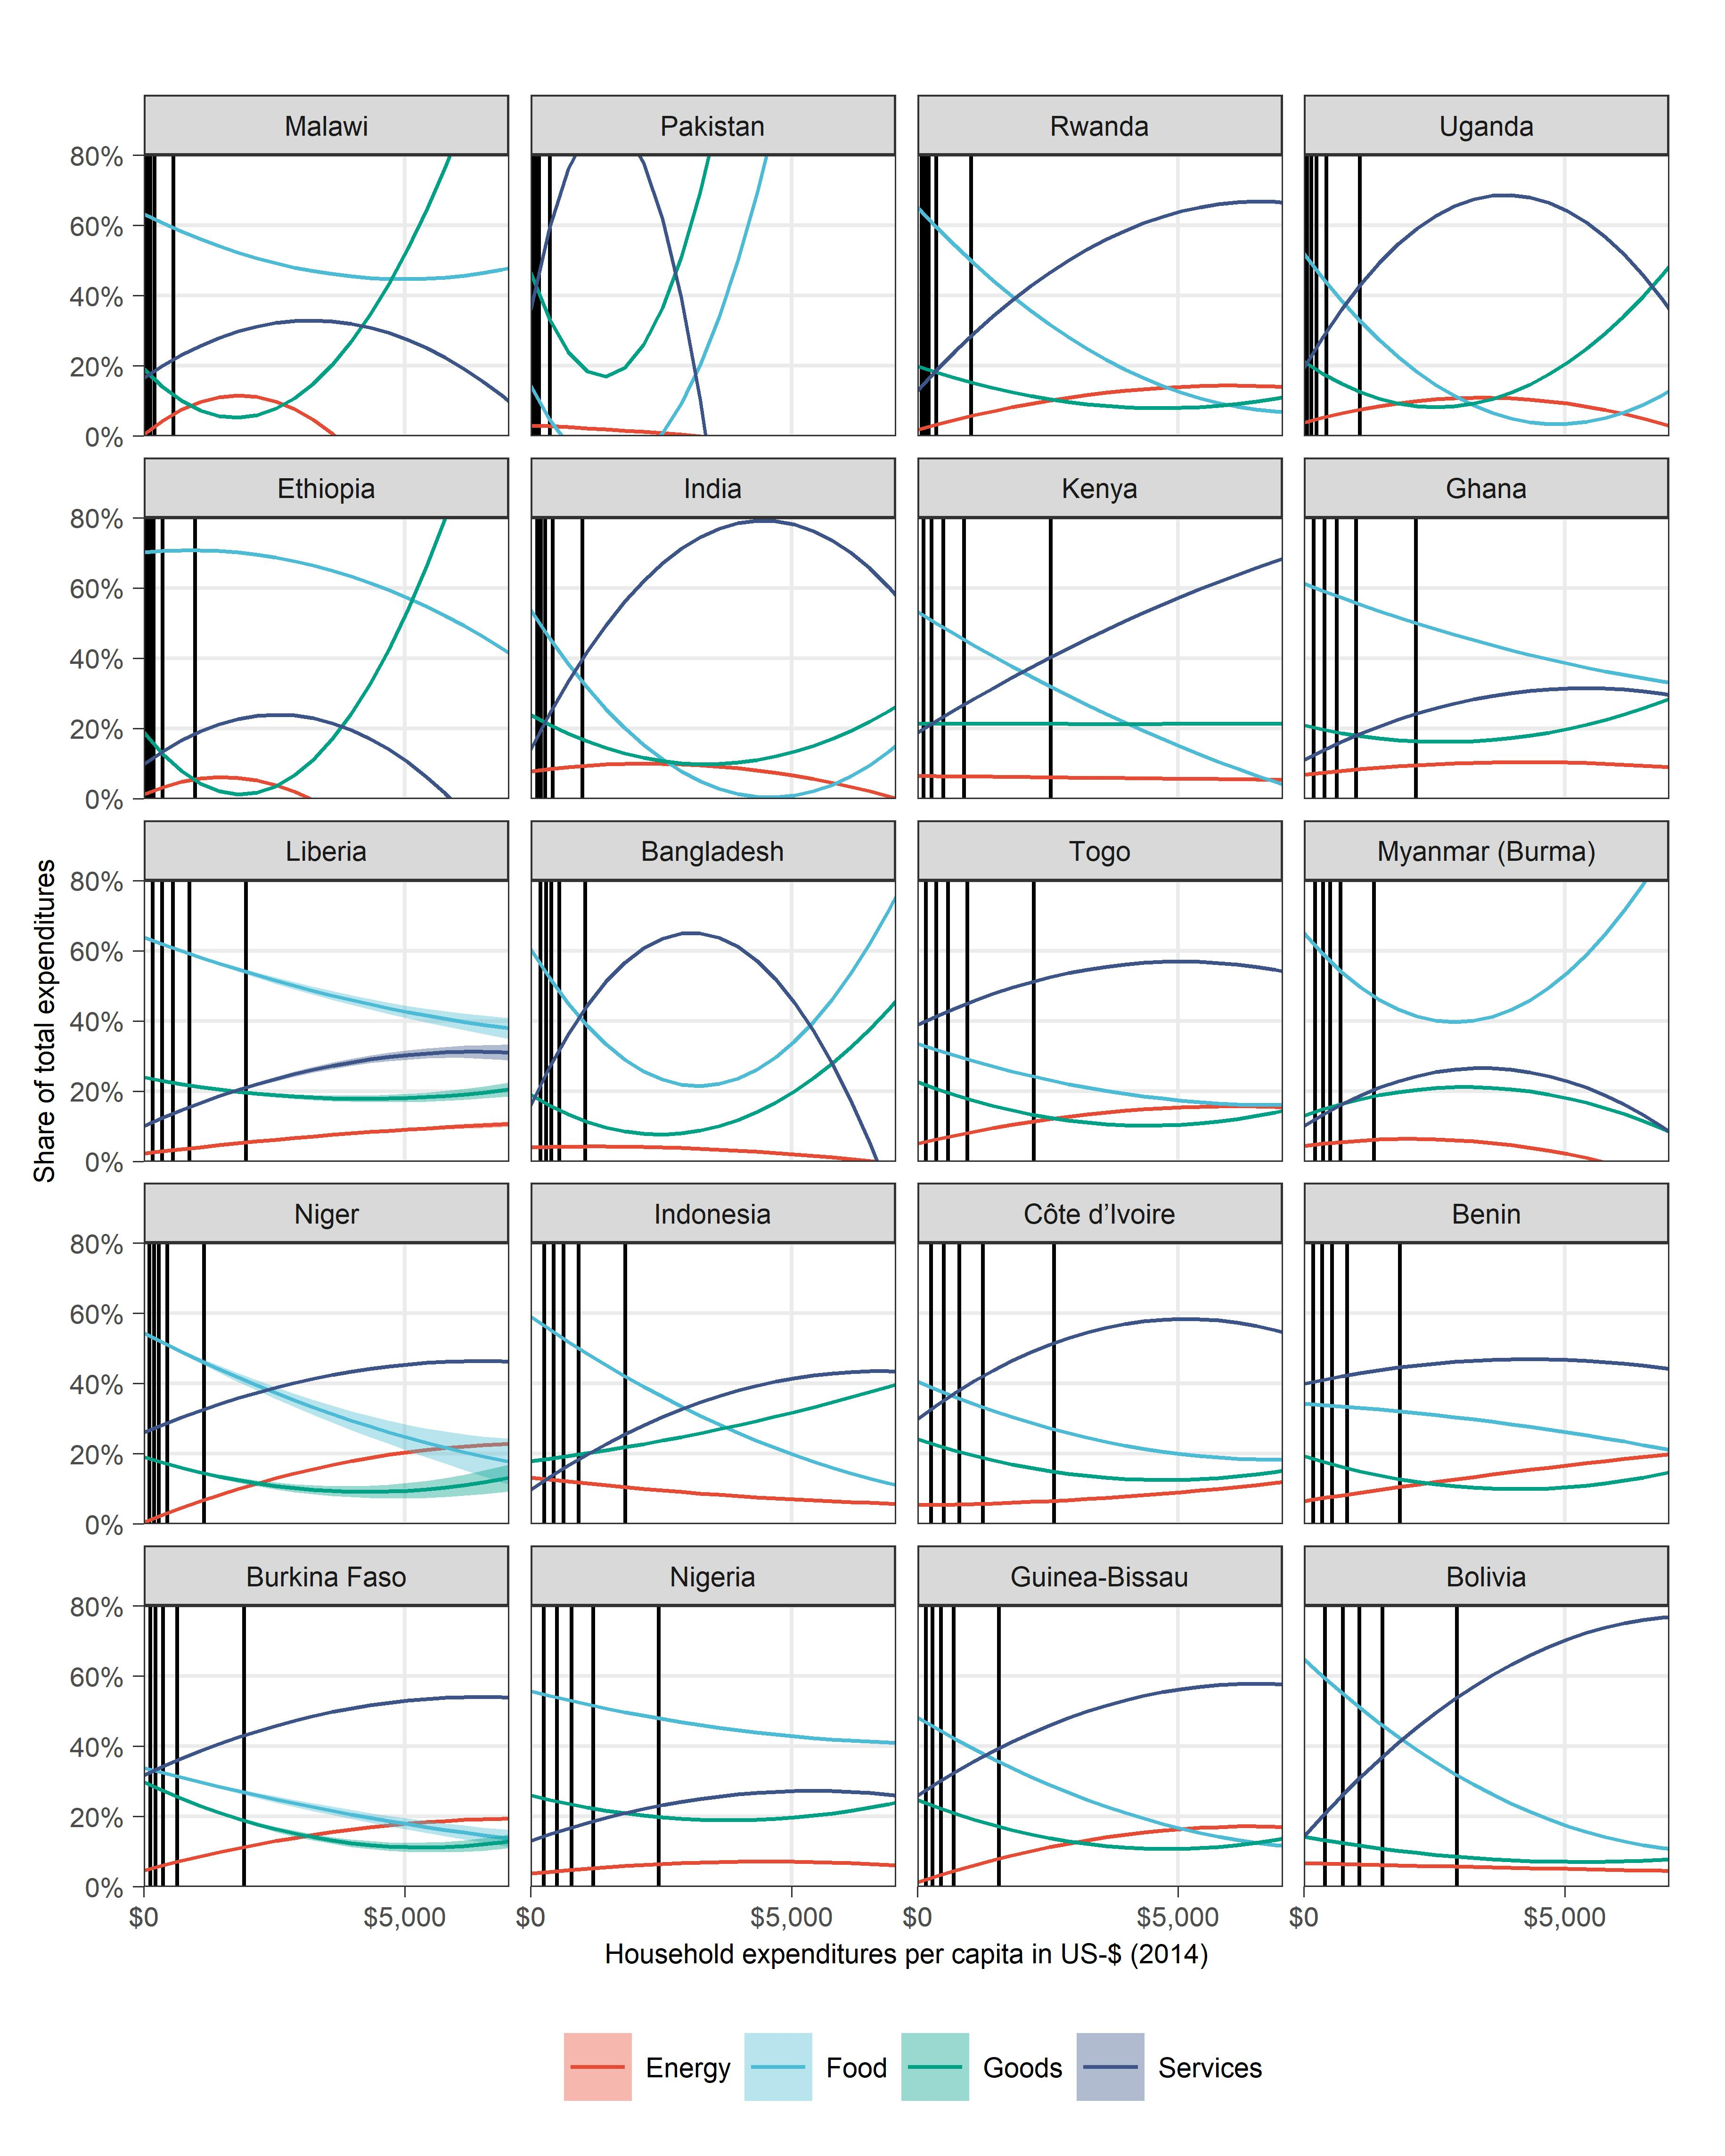
\includegraphics{Analysis_Parametric_Engel_Curves/Parametric_EC_0_A}
%   \begin{subcaption2}
%     This figure displays fitted lines for parametric and quadratic Engel curves for each consumption category in 20 countries of our sample. Black vertical lines indicate average household expenditures per capita for each expenditure quintile and country.
%   \end{subcaption2}

% \end{figure}

% \clearpage

% \begin{figure}[ht!]
%   \centering
%   \caption{Engel curves: expenditure shares over total household expenditures - Part B} \label{fig:A2}
%   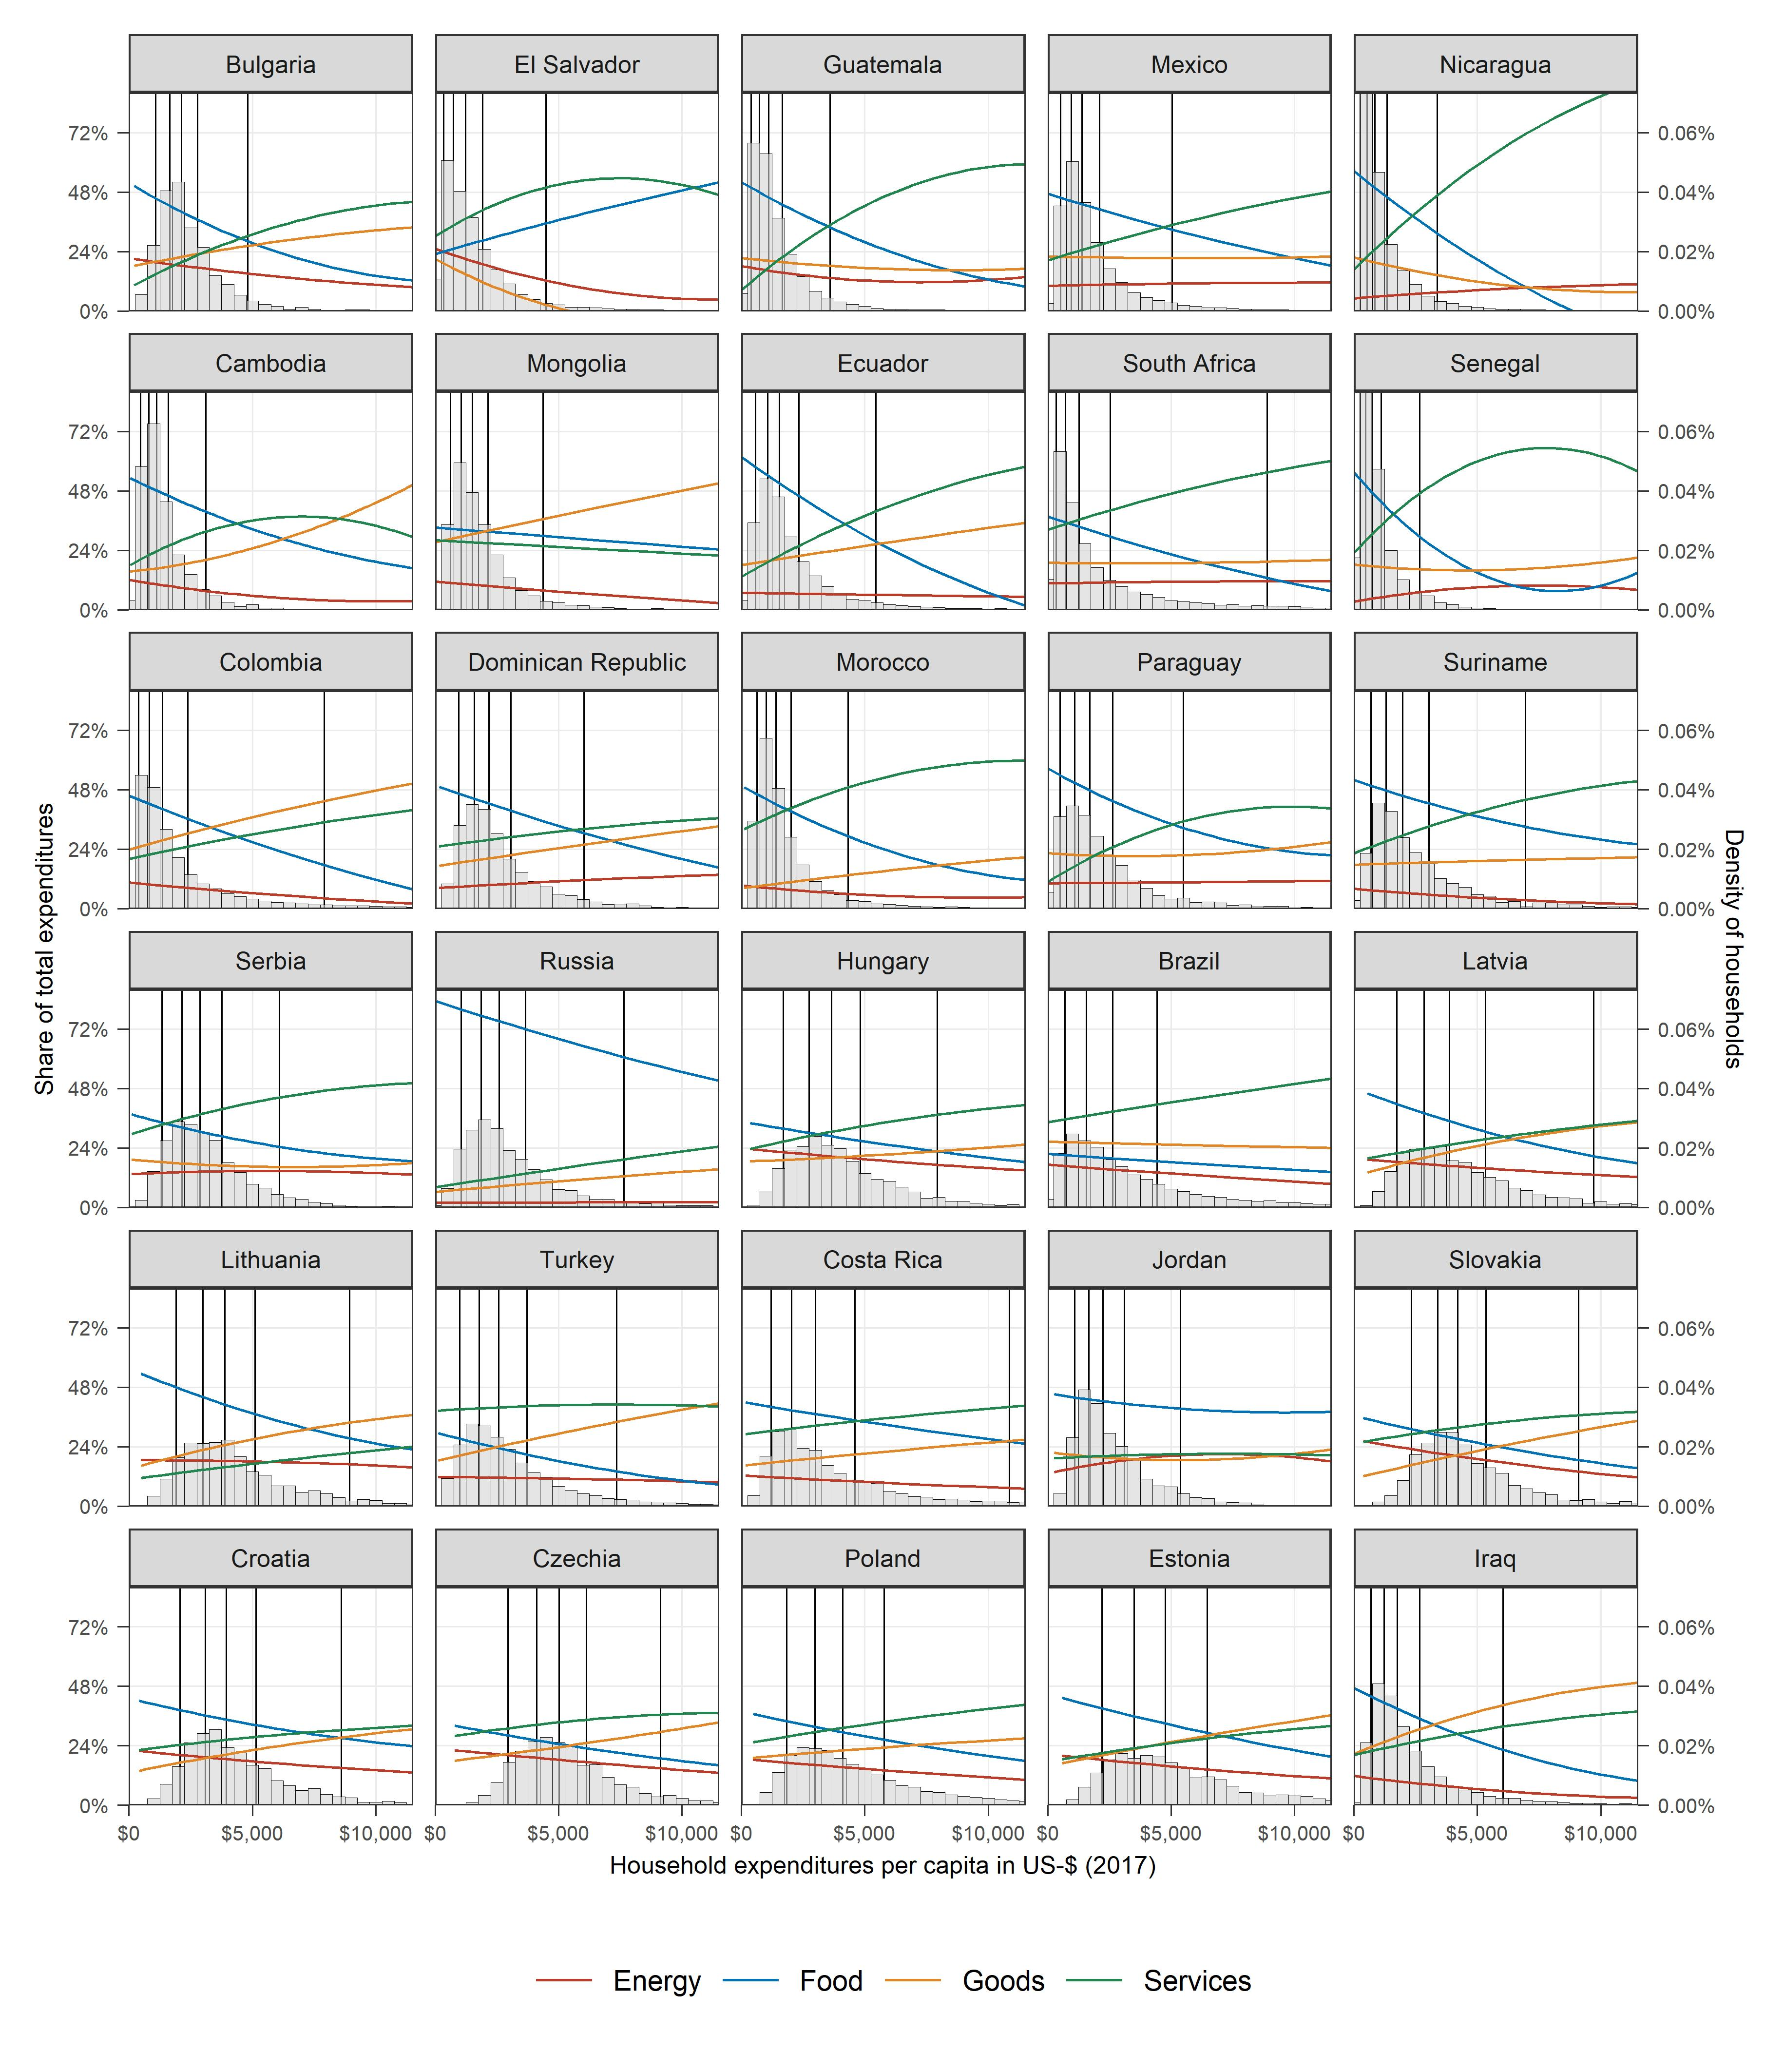
\includegraphics{Analysis_Parametric_Engel_Curves/Parametric_EC_0_B}
%   \begin{subcaption2}
%     This figure displays fitted lines for parametric and quadratic Engel curves for each consumption category in 20 countries of our sample. Black vertical lines indicate average household expenditures per capita for each expenditure quintile and country.
%   \end{subcaption2}

% \end{figure}

% \clearpage

% \begin{figure}[ht!]
%   \centering
%   \caption{Engel curves: expenditure shares over total household expenditures - Part C} \label{fig:A3}
%   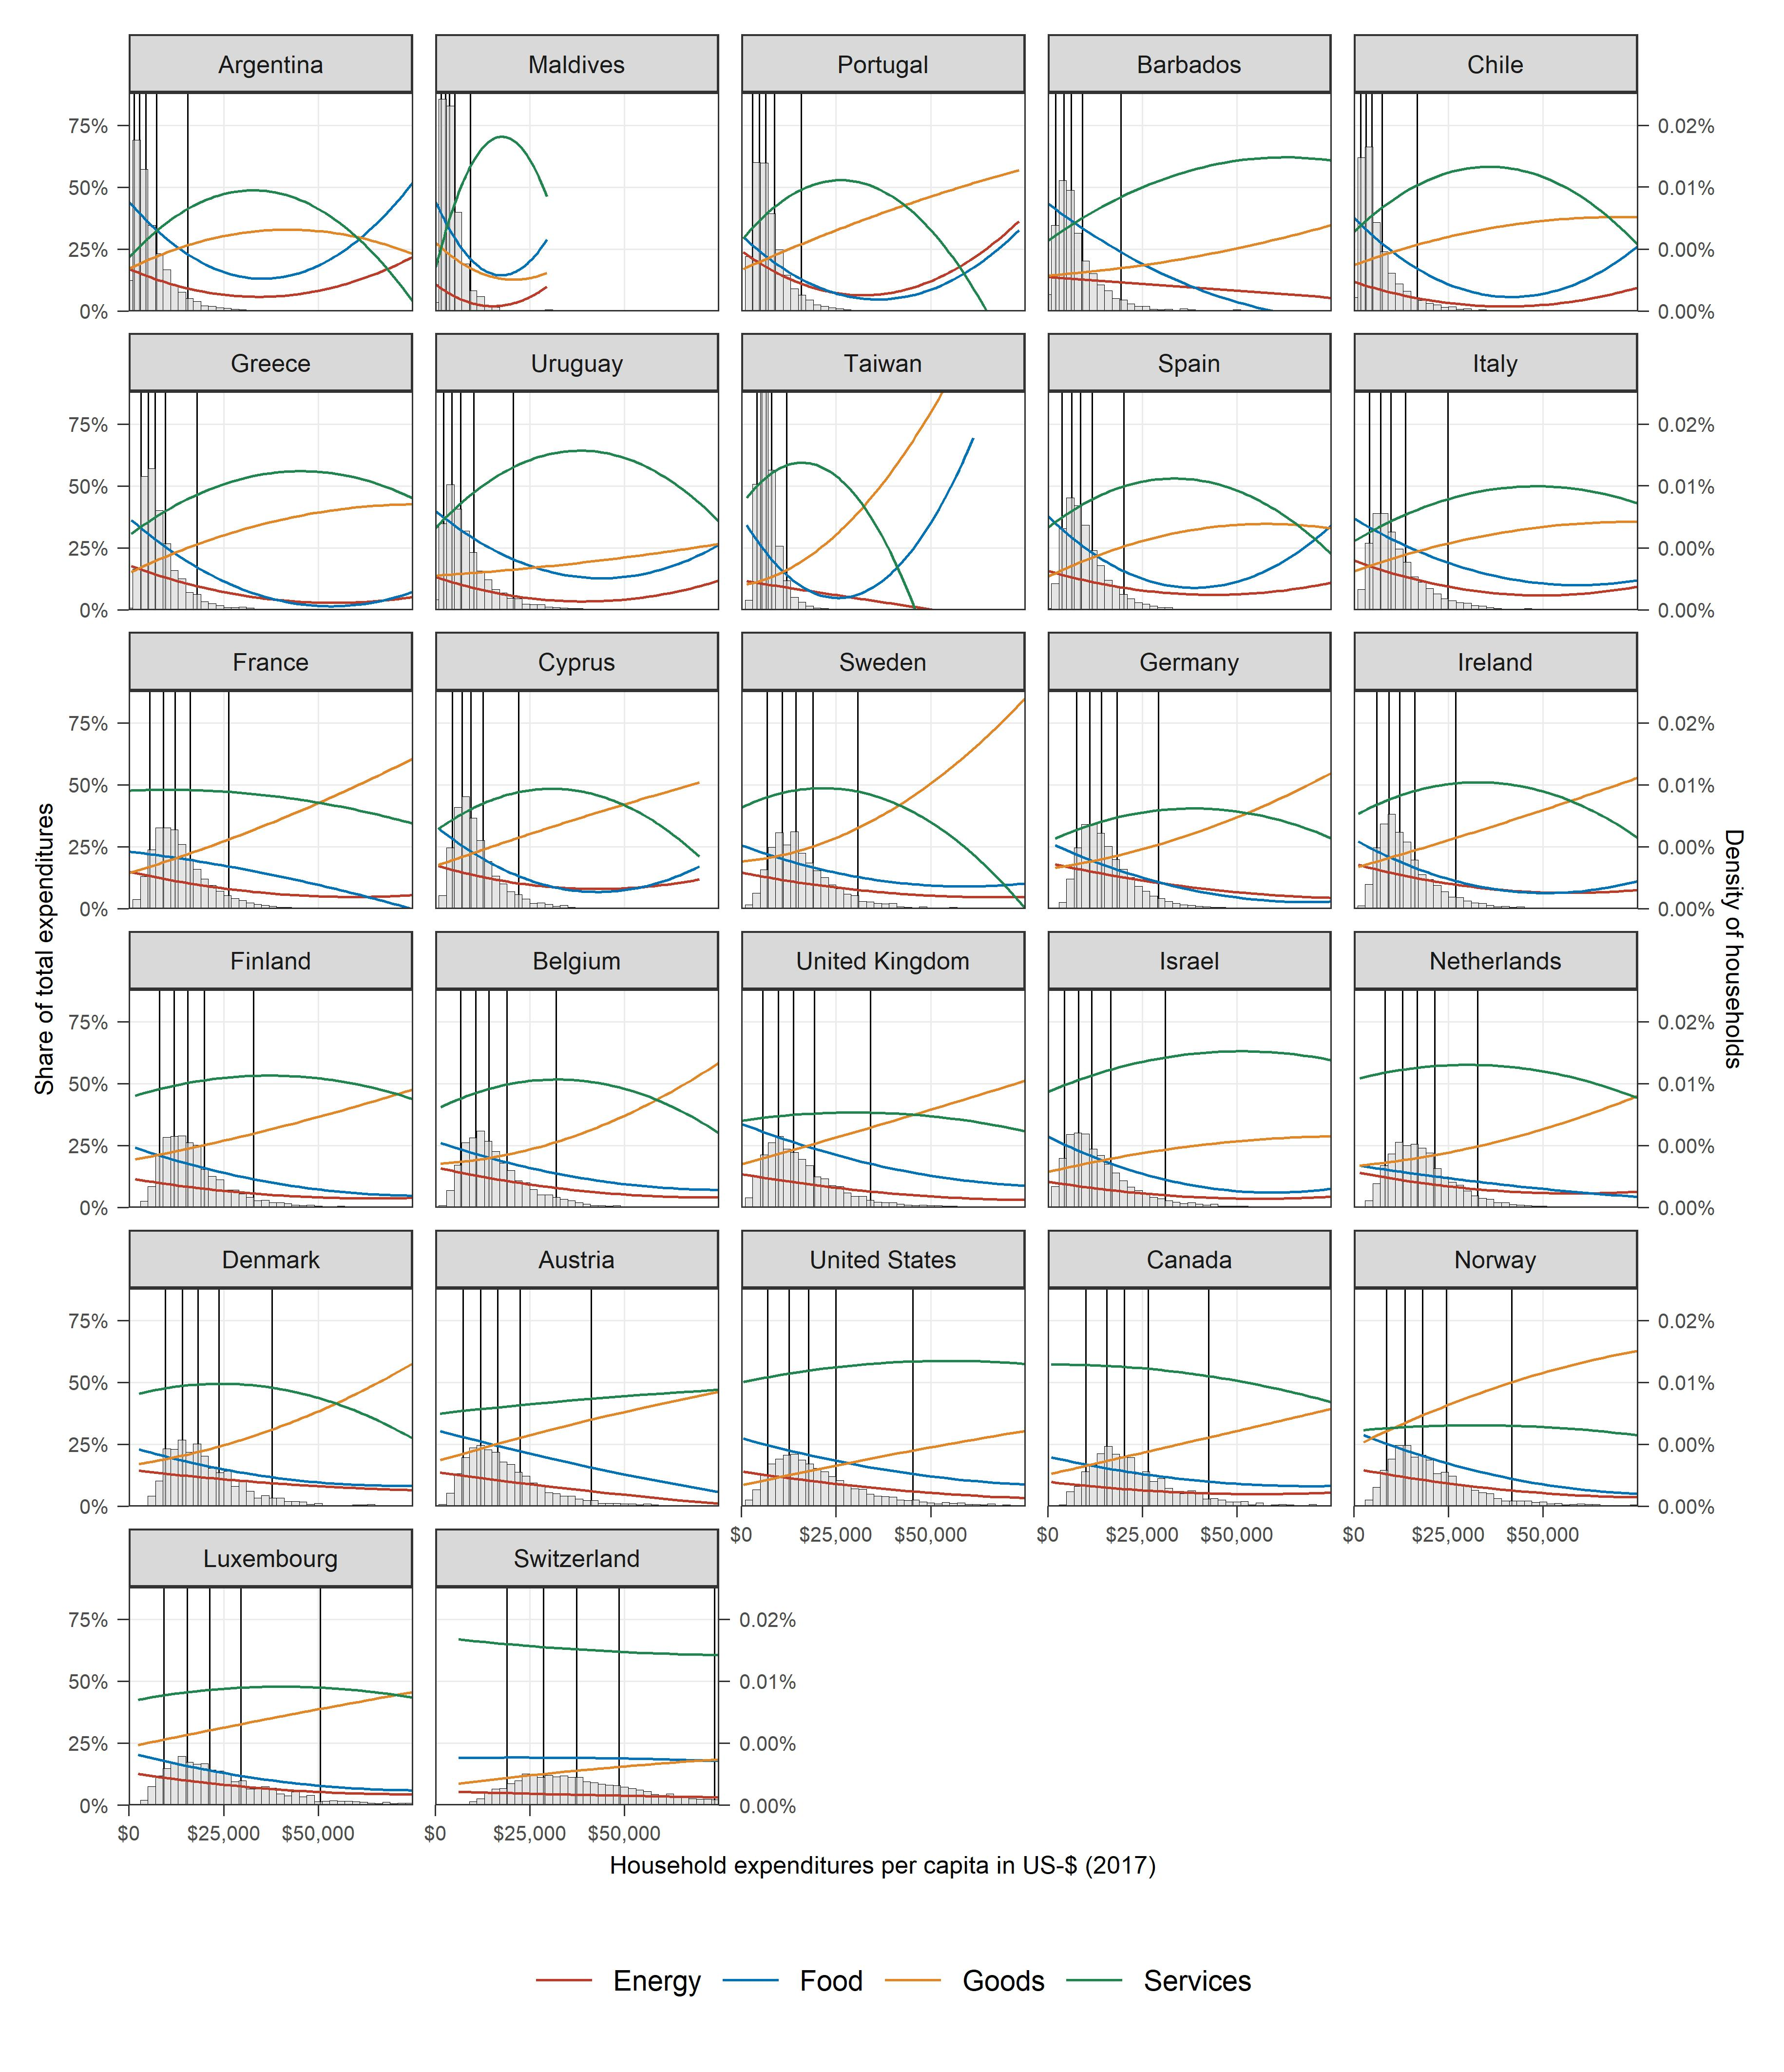
\includegraphics{Analysis_Parametric_Engel_Curves/Parametric_EC_0_C}
%   \begin{subcaption2}
%     This figure displays fitted lines for parametric and quadratic Engel curves for each consumption category in 20 countries of our sample. Black vertical lines indicate average household expenditures per capita for each expenditure quintile and country.
%   \end{subcaption2}

% \end{figure}

% \clearpage

% \begin{figure}[ht!]
%   \centering
%   \caption{Engel curves: expenditure shares over total household expenditures - Part D} \label{fig:A4}
%   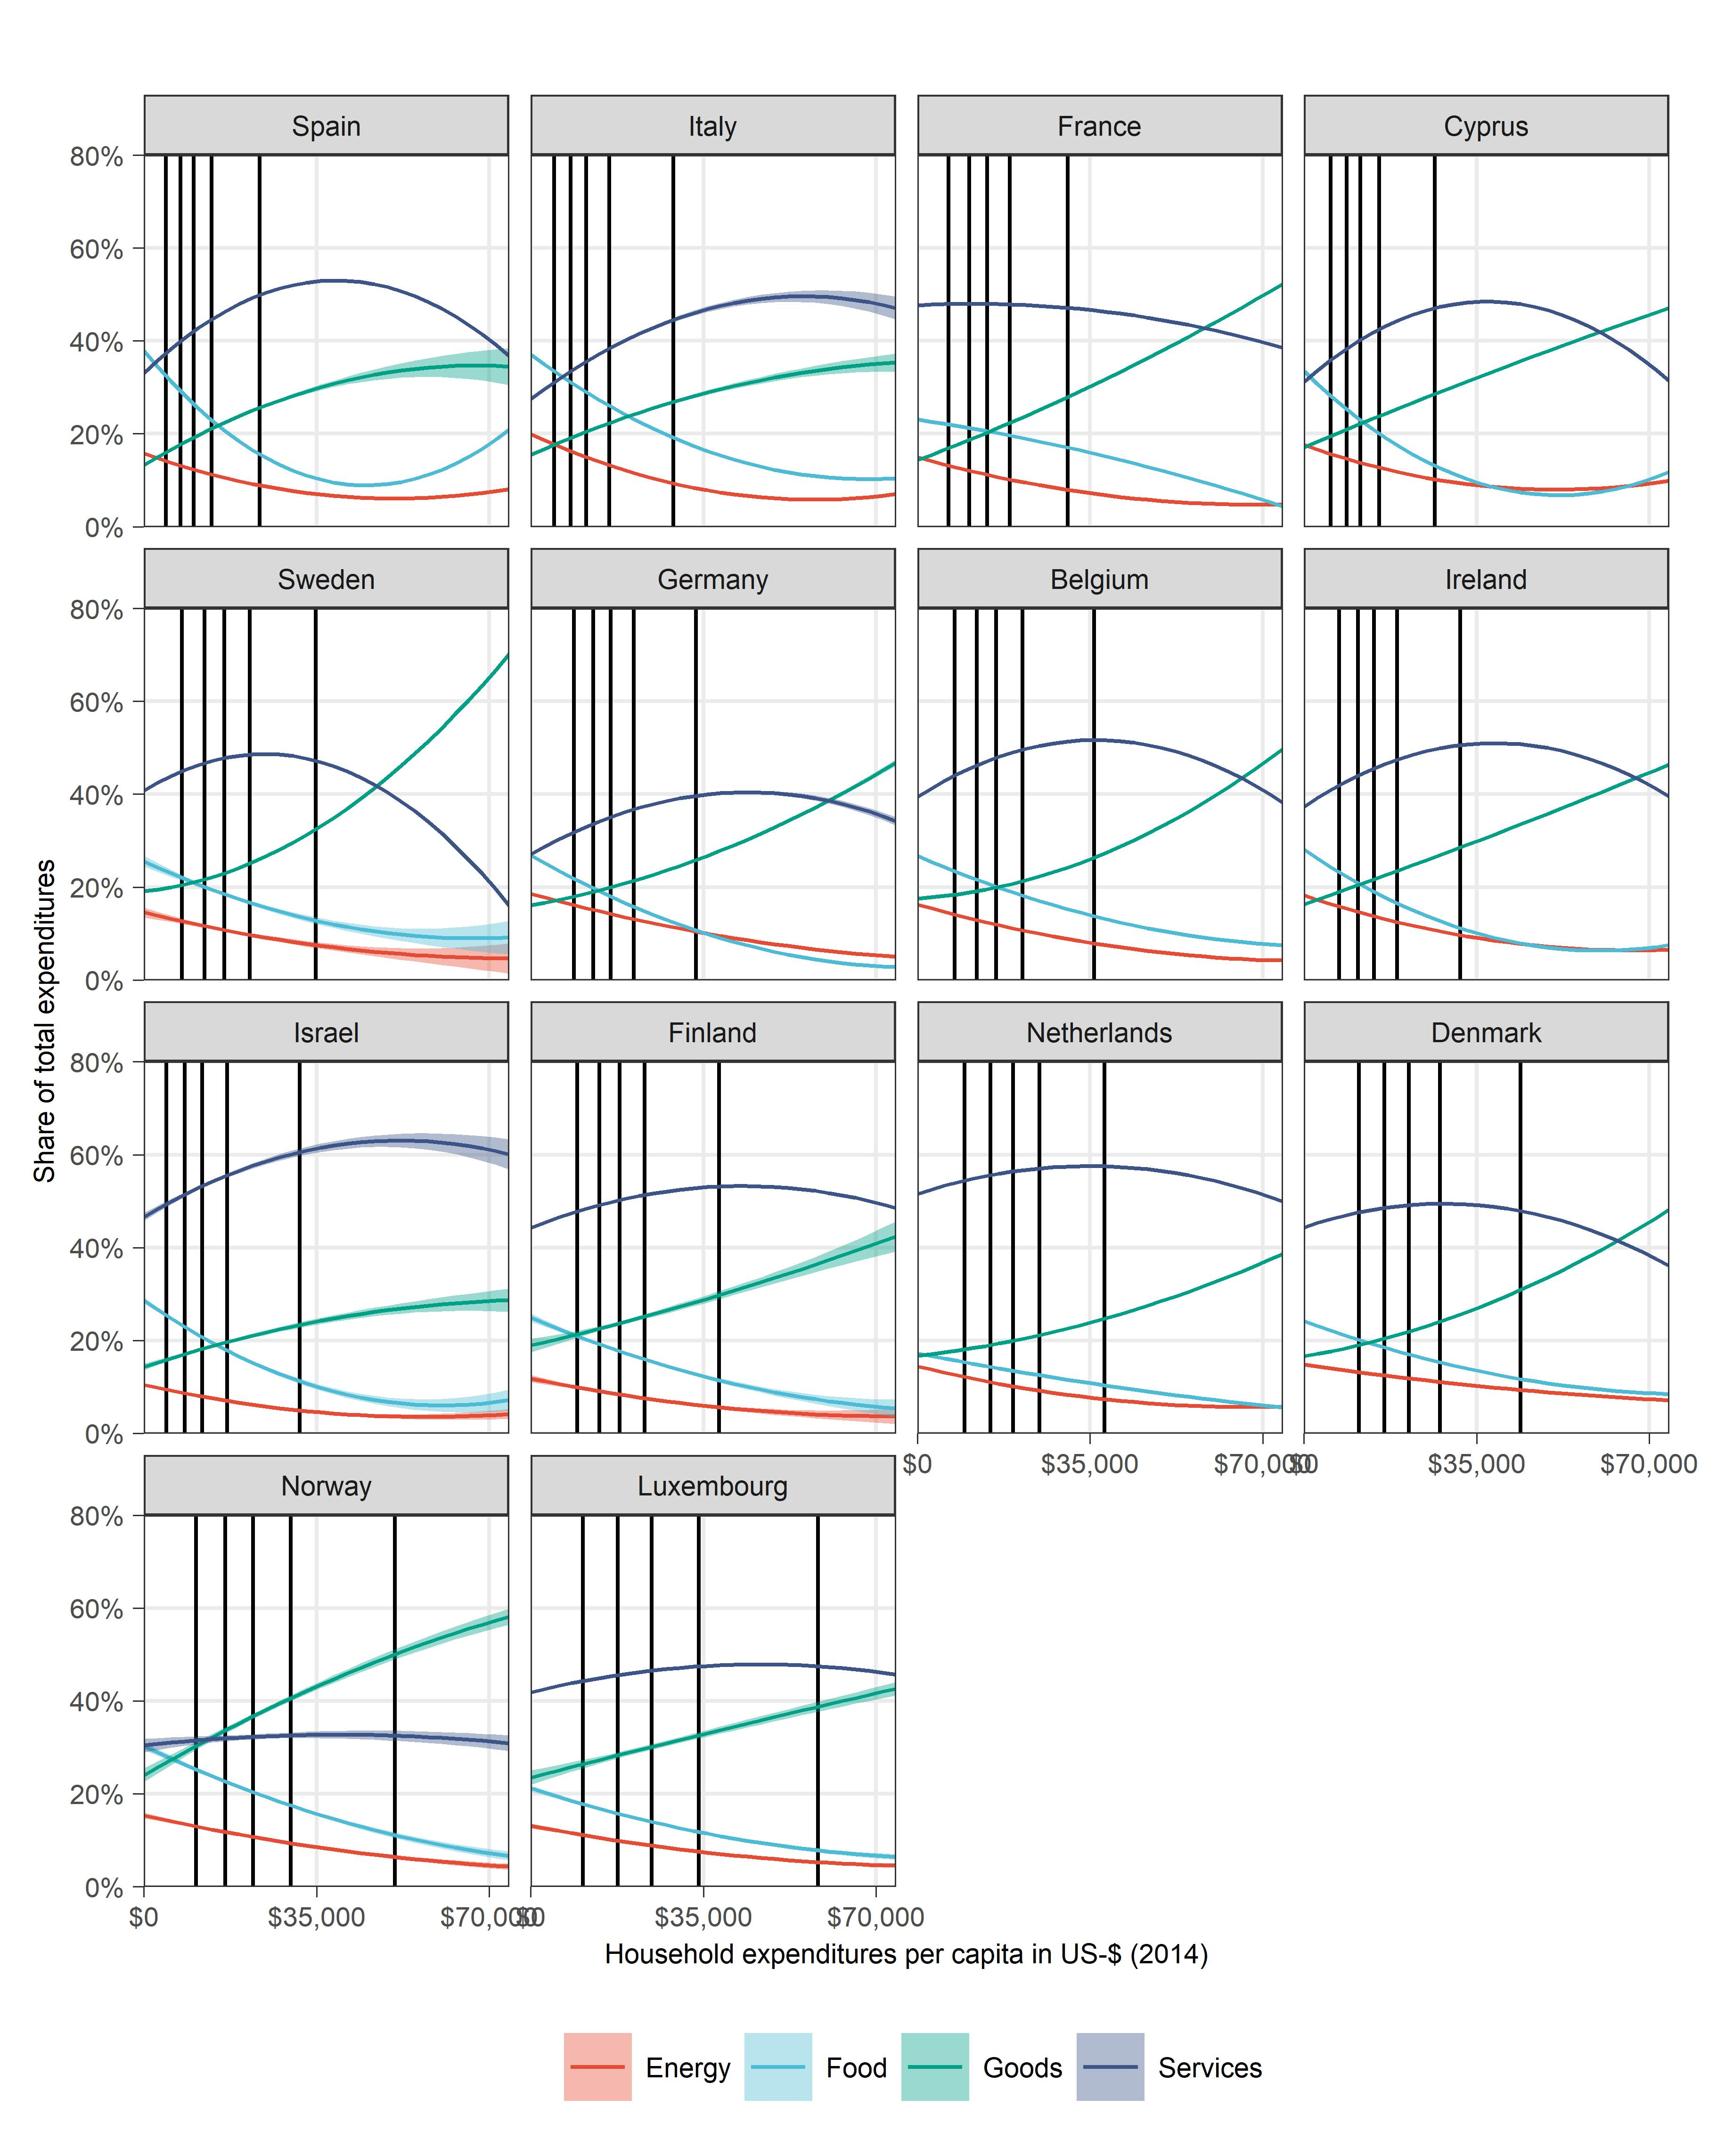
\includegraphics{Analysis_Parametric_Engel_Curves/Parametric_EC_0_D}
%   \begin{subcaption2}
%     This figure displays fitted lines for parametric and quadratic Engel curves for each consumption category in 20 countries of our sample. Black vertical lines indicate average household expenditures per capita for each expenditure quintile and country.
%   \end{subcaption2}

% \end{figure}

% \clearpage

% Carbon intensities

\begin{figure}[ht!]
  \centering
  \caption{Sectoral carbon intensities from GTAP - Part A} \label{fig:B1}
  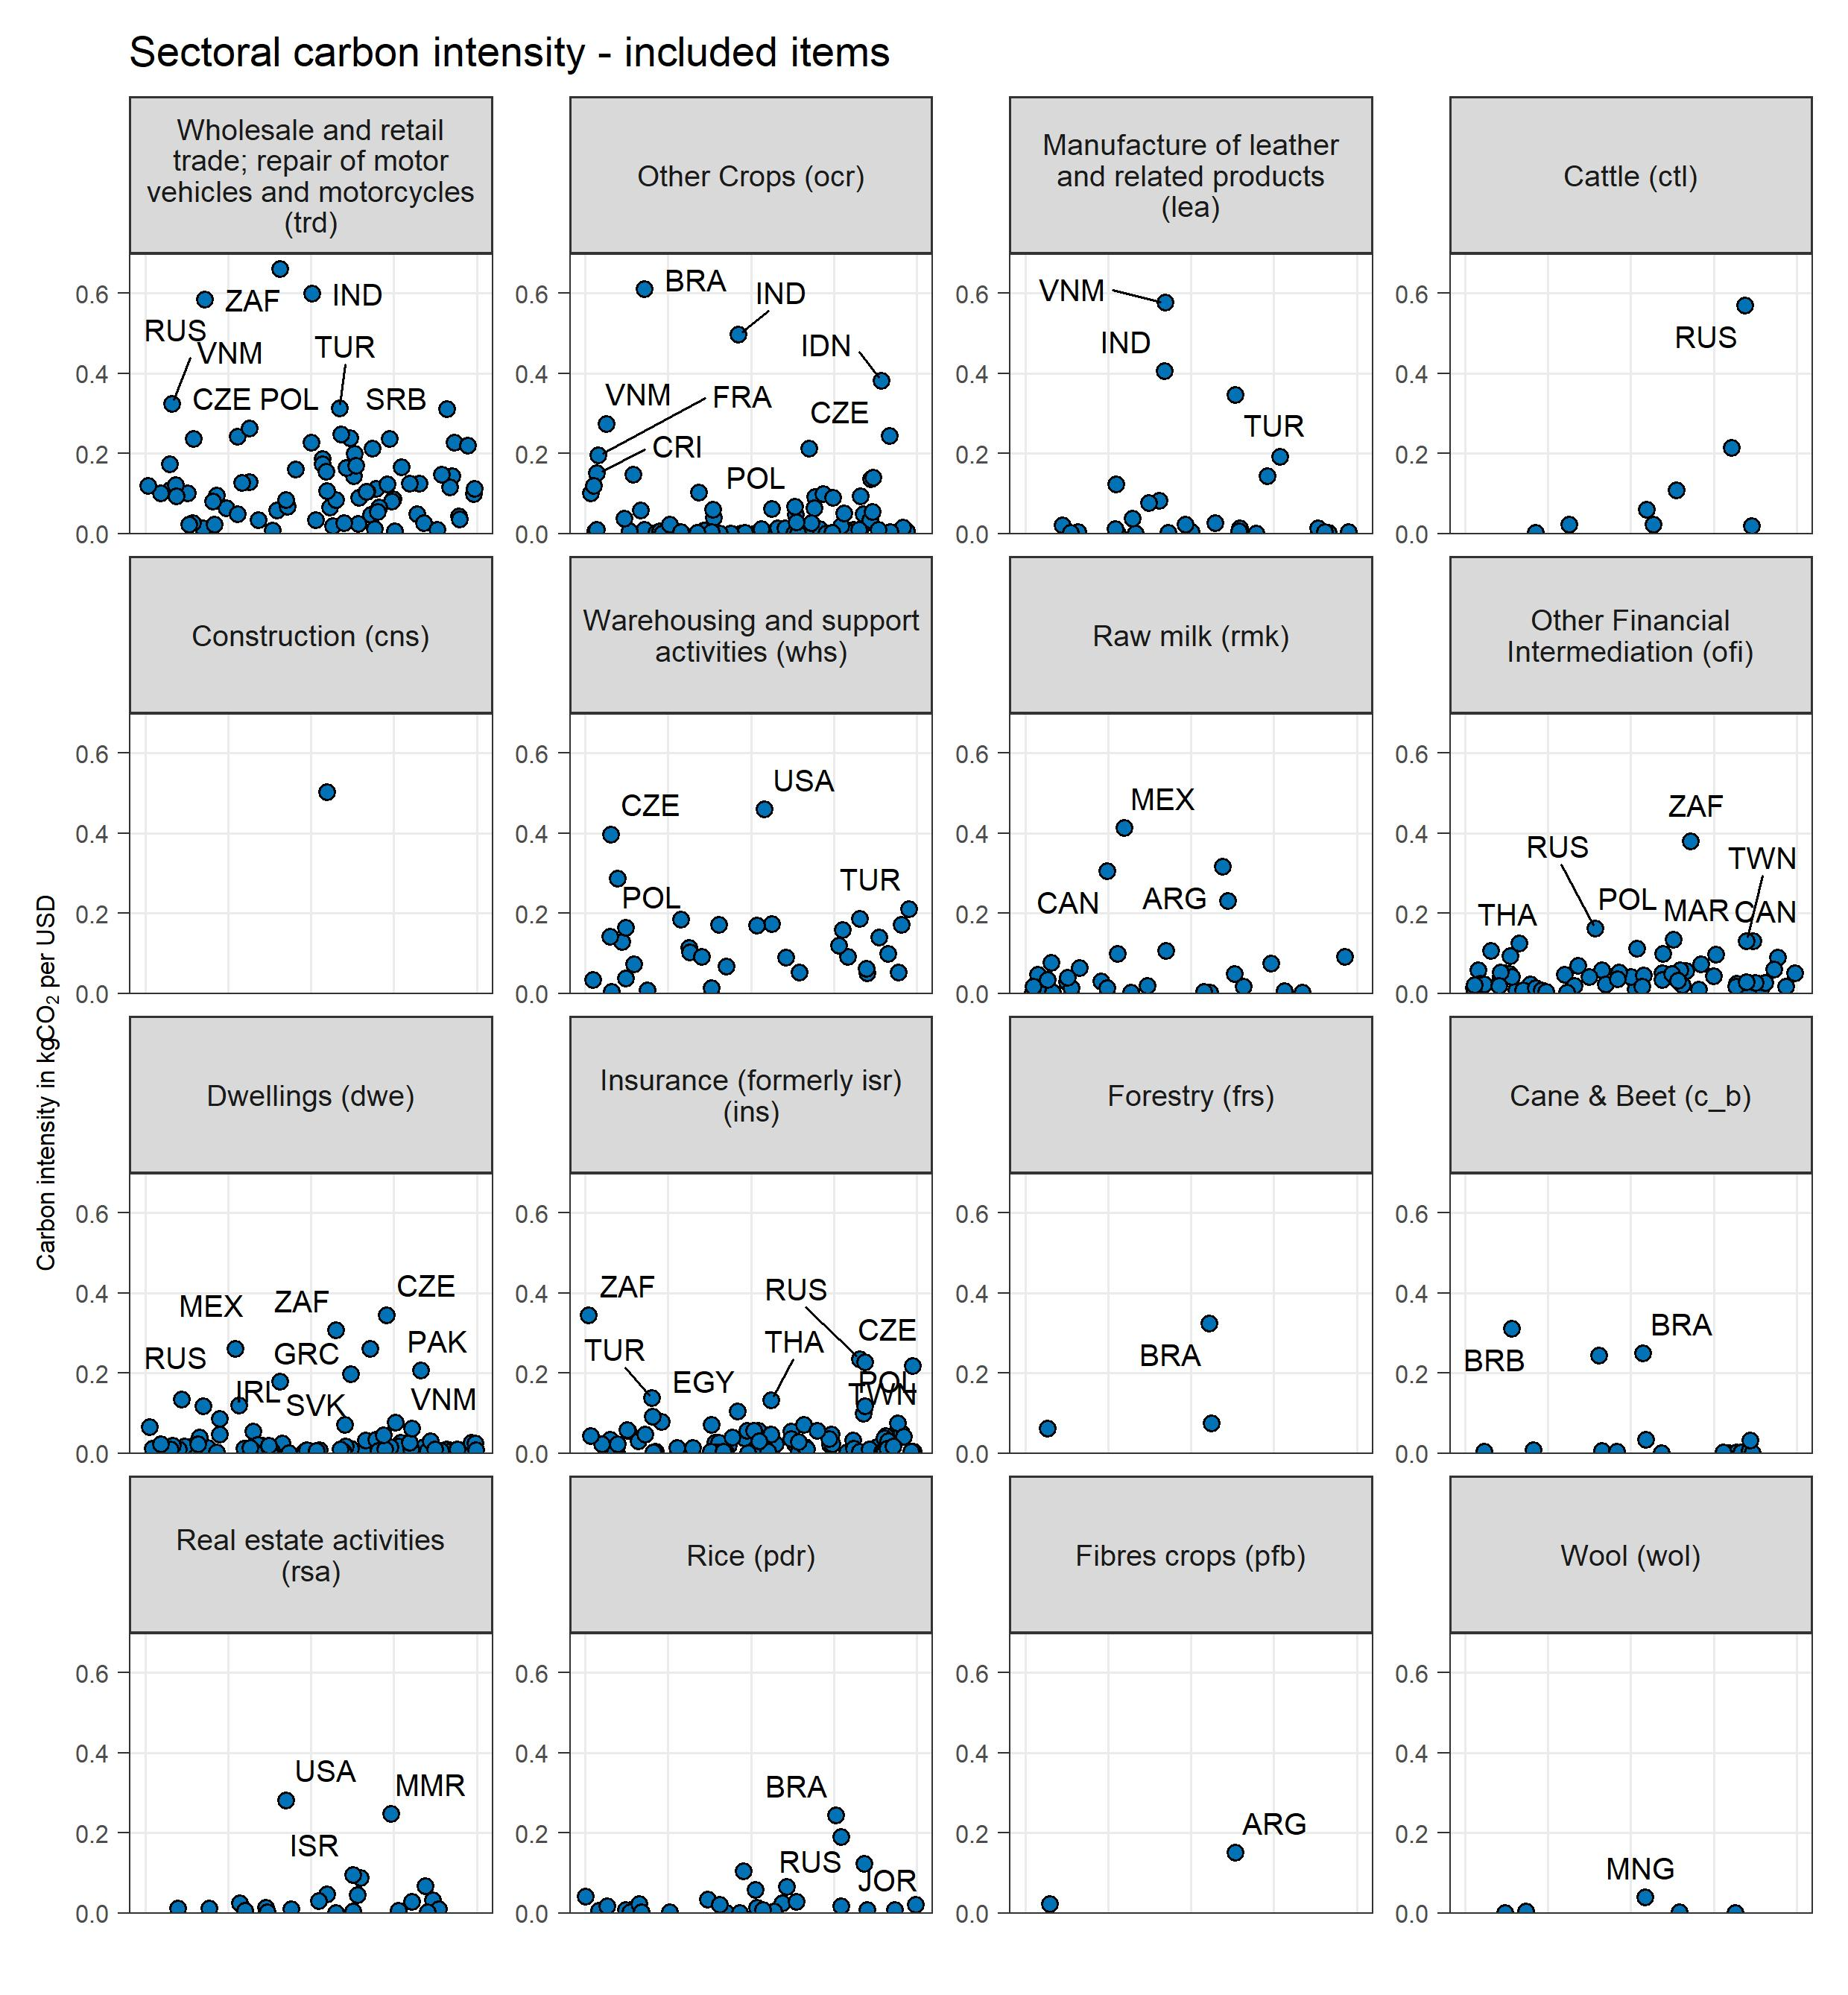
\includegraphics{Analysis_Carbon_Intensities_GTAP/Figure_2.1.1_A_2017}
  \begin{subcaption2}
    This figure displays sectoral carbon intensities in kgCO$_{2}$ per USD of output for 16 sectors. We plot sectoral carbon intensities if household budget surveys in respective countries include consumption items which correspond to each sector. See our online repository for all country- and sector-level carbon intensities. We include labels with country codes if sector outputs are relatively carbon-intensive compared to other countries. See also Figures \ref{fig:B2}, \ref{fig:B3} and \ref{fig:B4}. Note that sectors \textit{other mining extraction (oxt)} and \textit{extraction of crude petroleum (oil)} are not matched to any item in any country.
  \end{subcaption2}

\end{figure}

\clearpage

\begin{figure}[ht!]
  \centering
  \caption{Sectoral carbon intensities from GTAP - Part B} \label{fig:B2}
  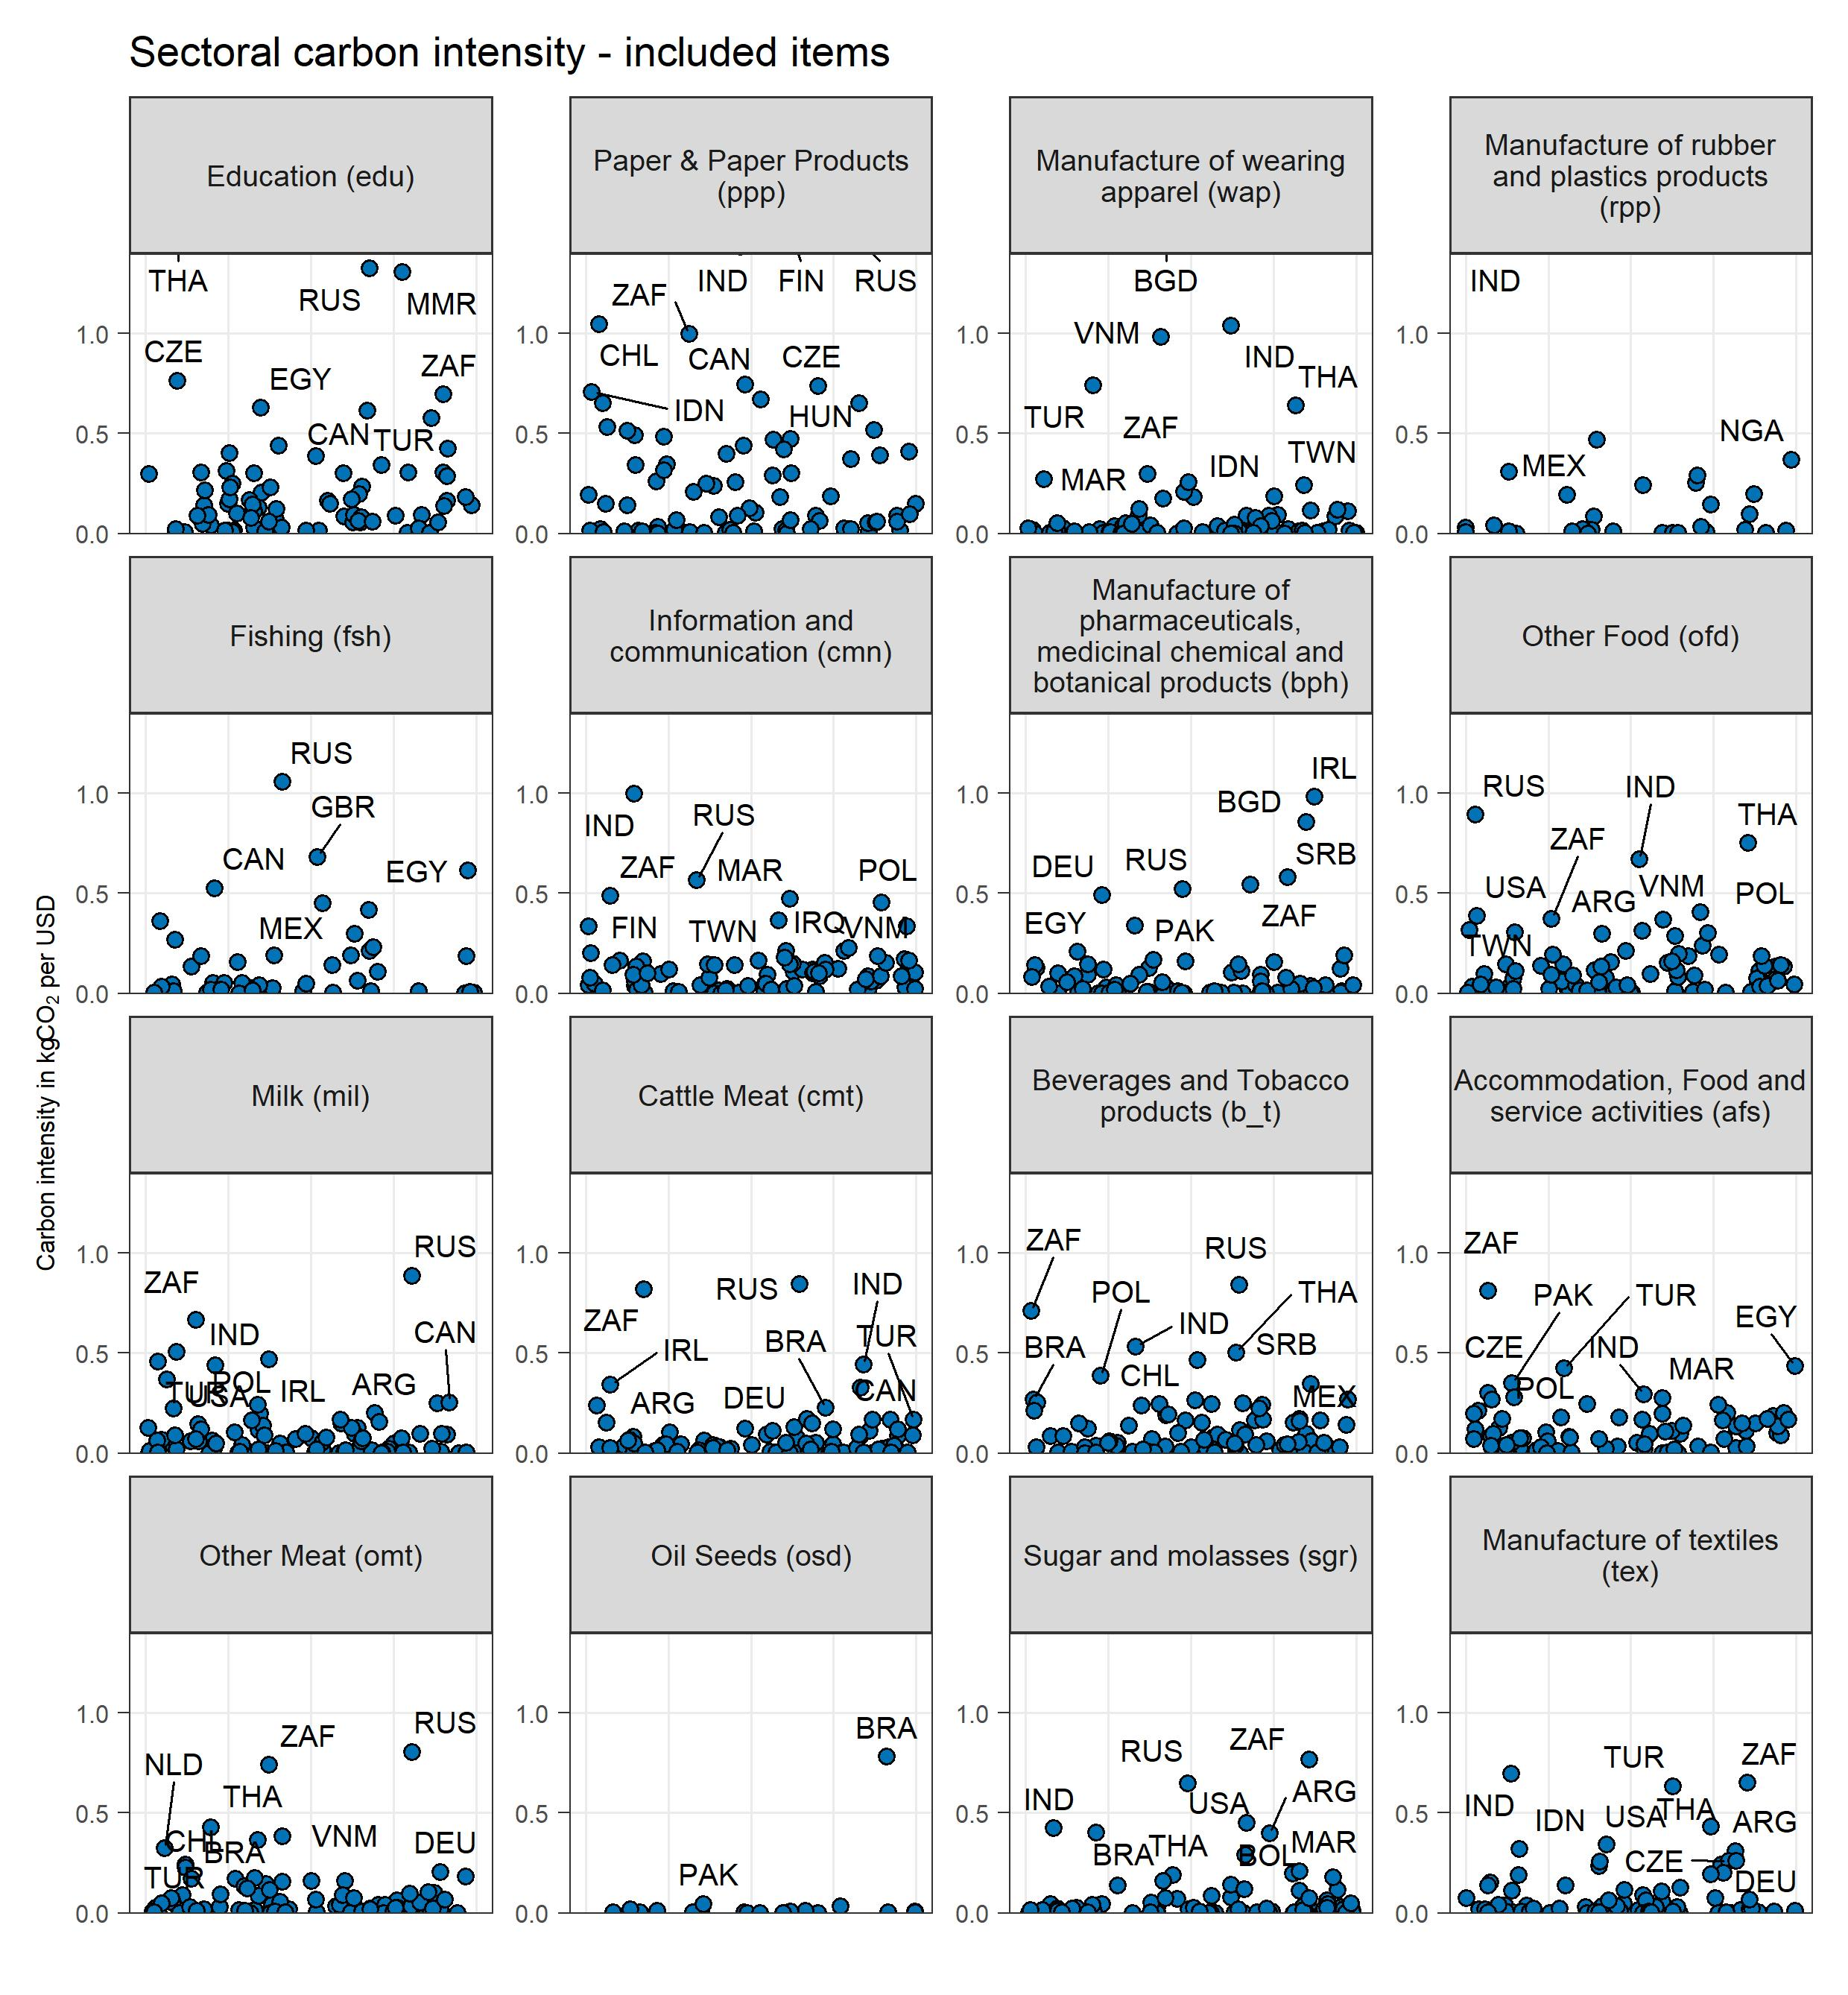
\includegraphics{Analysis_Carbon_Intensities_GTAP/Figure_2.1.1_B_2017}
  \begin{subcaption2}
    This figure displays sectoral carbon intensities in kgCO$_{2}$ per USD of output for 16 sectors. We plot sectoral carbon intensities if household budget surveys in respective countries include consumption items which correspond to each sector. See our online repository for all country- and sector-level carbon intensities. We include labels with country codes if sector outputs are relatively carbon-intensive compared to other countries. See also Figures \ref{fig:B1}, \ref{fig:B3} and \ref{fig:B4}. Note that sectors \textit{other mining extraction (oxt)} and \textit{extraction of crude petroleum (oil)} are not matched to any item in any country.
  \end{subcaption2}

\end{figure}

\clearpage

\begin{figure}[ht!]
  \centering
  \caption{Sectoral carbon intensities from GTAP - Part C} \label{fig:B3}
  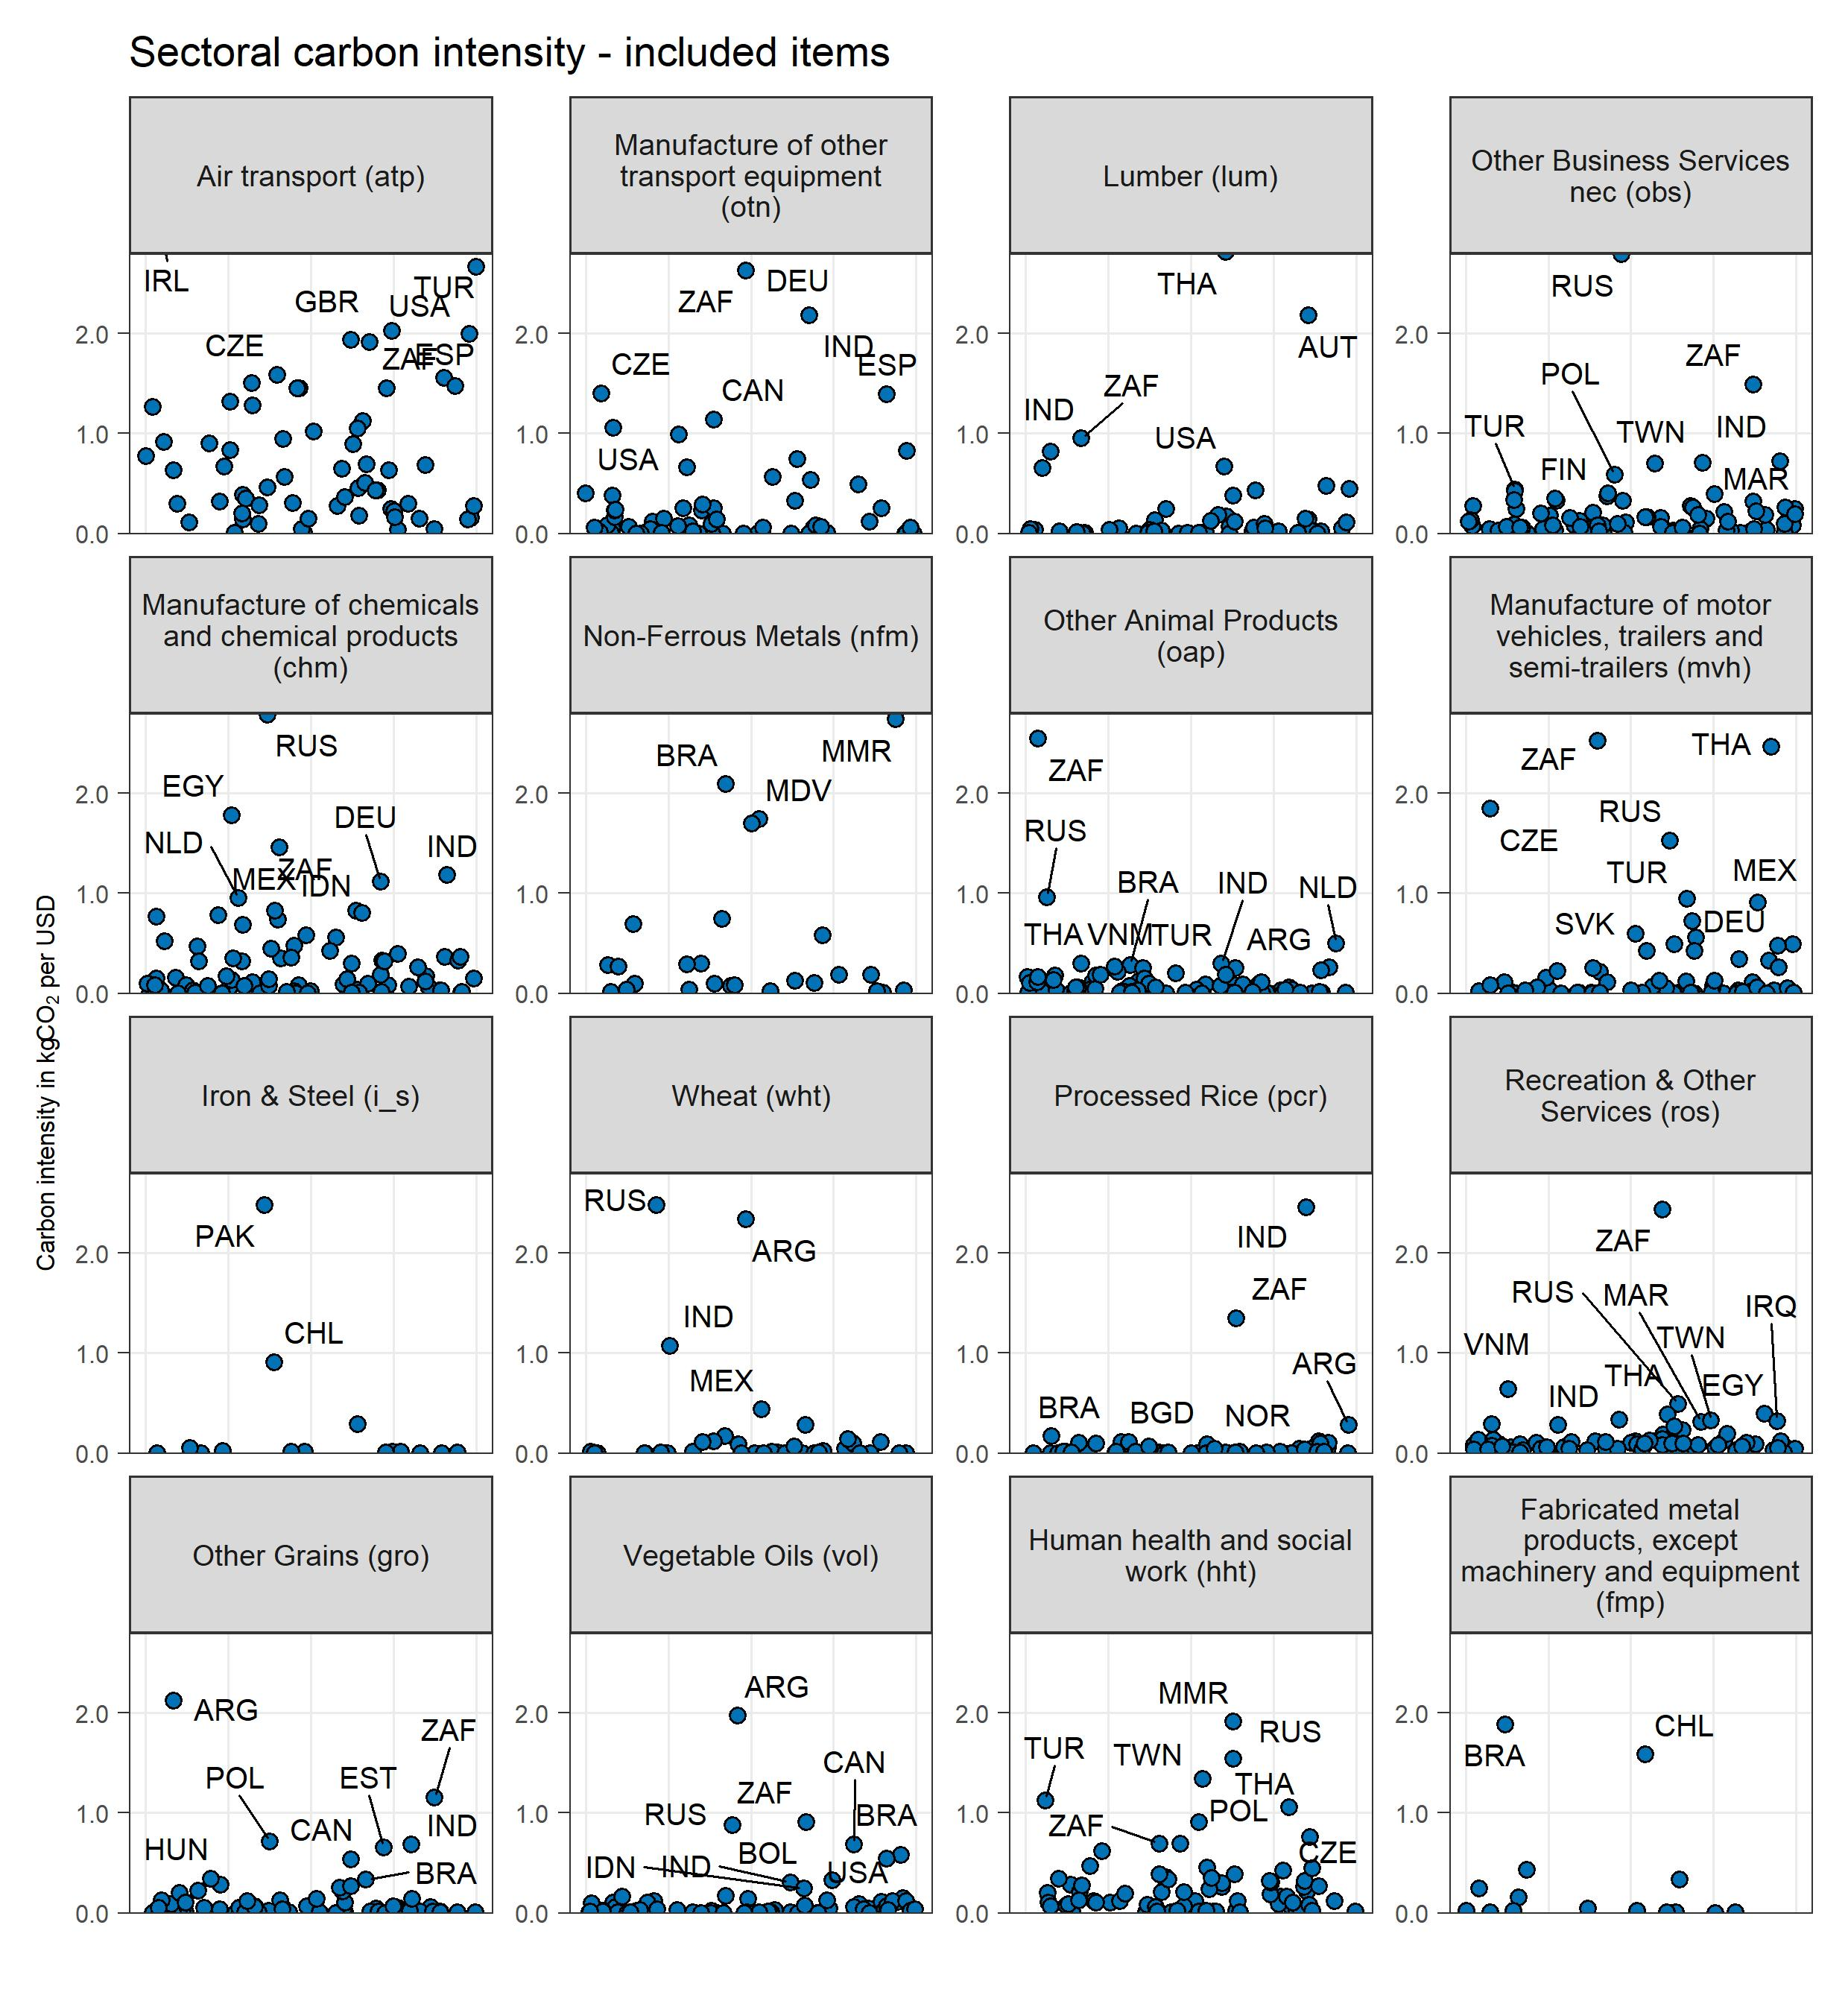
\includegraphics{Analysis_Carbon_Intensities_GTAP/Figure_2.1.1_C_2017}
  \begin{subcaption2}
    This figure displays sectoral carbon intensities in kgCO$_{2}$ per USD of output for 16 sectors. We plot sectoral carbon intensities if household budget surveys in respective countries include consumption items which correspond to each sector. See our online repository for all country- and sector-level carbon intensities. We include labels with country codes if sector outputs are relatively carbon-intensive compared to other countries. See also Figures \ref{fig:B1}, \ref{fig:B2} and \ref{fig:B4}. Note that sectors \textit{other mining extraction (oxt)} and \textit{extraction of crude petroleum (oil)} are not matched to any item in any country.
  \end{subcaption2}

\end{figure}

\clearpage

\begin{figure}[ht!]
  \centering
  \caption{Sectoral carbon intensities from GTAP - Part D} \label{fig:B4}
  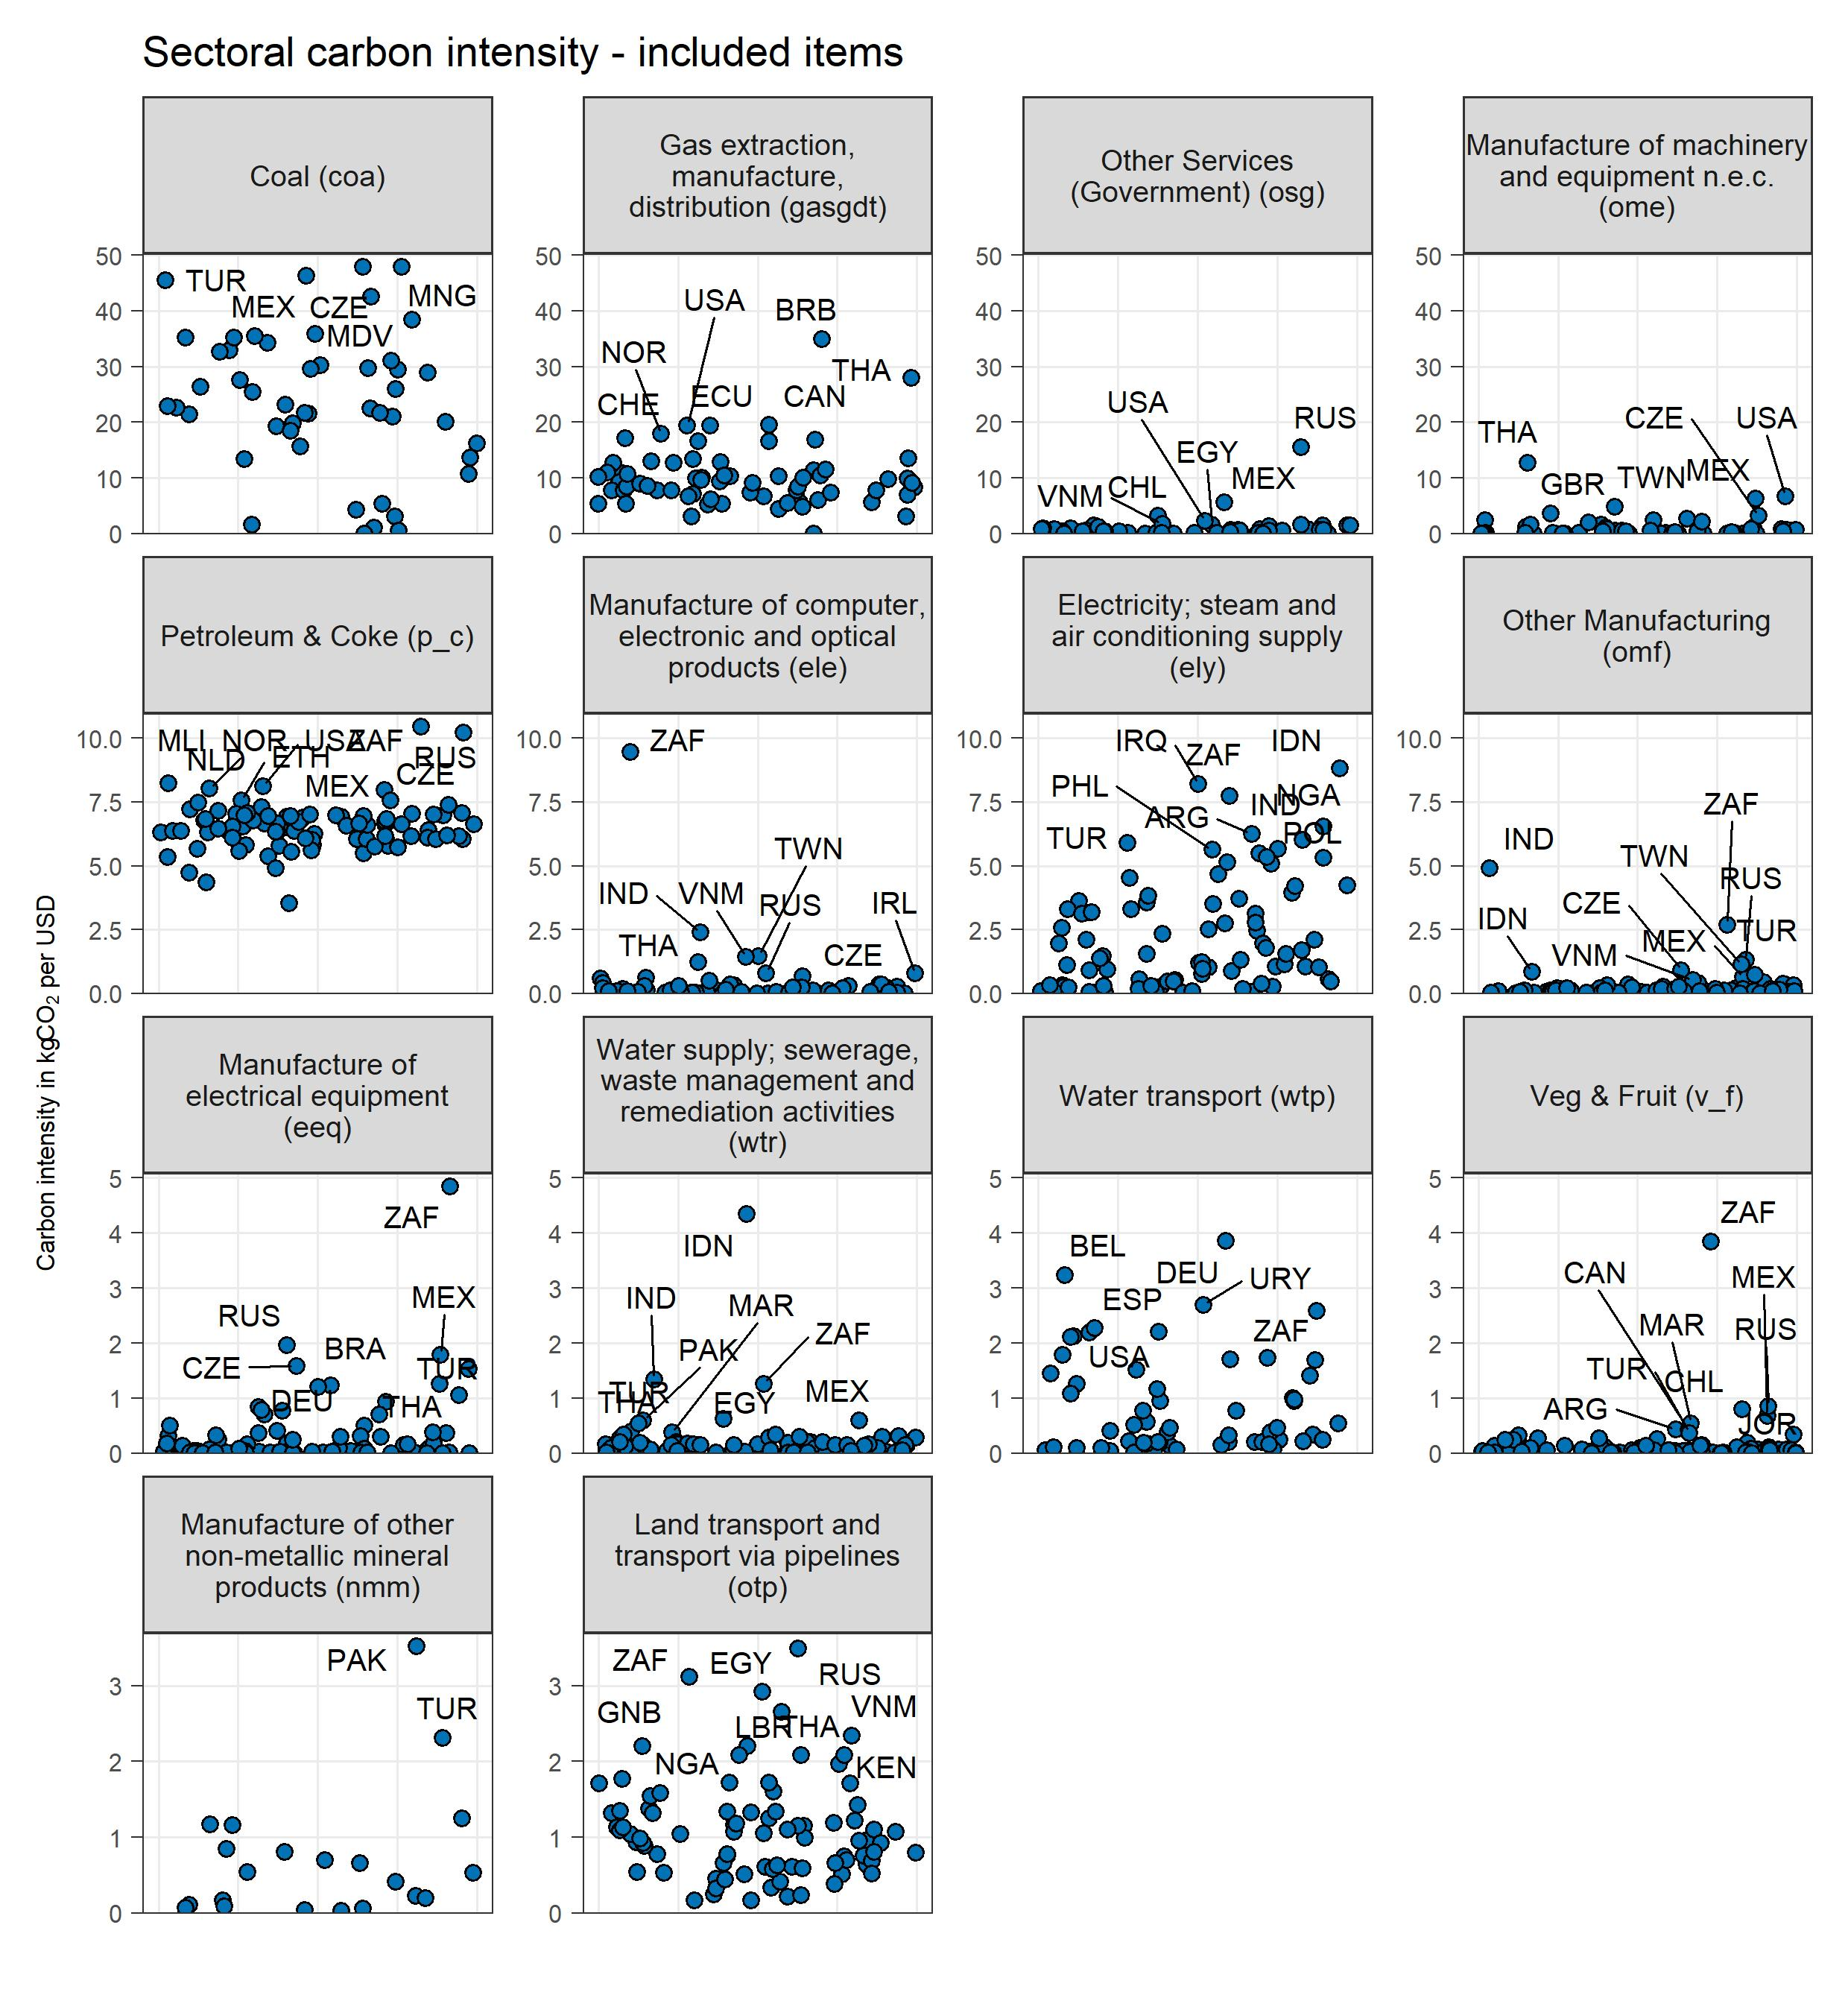
\includegraphics{Analysis_Carbon_Intensities_GTAP/Figure_2.1.1_D_2017}
  \begin{subcaption2}
    This figure displays sectoral carbon intensities in kgCO$_{2}$ per USD of output for 14 sectors. We plot sectoral carbon intensities if household budget surveys in respective countries include consumption items which correspond to each sector. See our online repository for all country- and sector-level carbon intensities. We include labels with country codes if sector outputs are relatively carbon-intensive compared to other countries. See also Figures \ref{fig:B1}, \ref{fig:B2} and \ref{fig:B3}. Note that sectors \textit{other mining extraction (oxt)} and \textit{extraction of crude petroleum (oil)} are not matched to any item in any country.
  \end{subcaption2}

\end{figure}

\clearpage

% Boxplots over quintiles

\begin{figure}[ht!]
  \centering
  \caption{Distribution of carbon intensities over expenditure quintiles - Part A} \label{fig:Quint_A}
  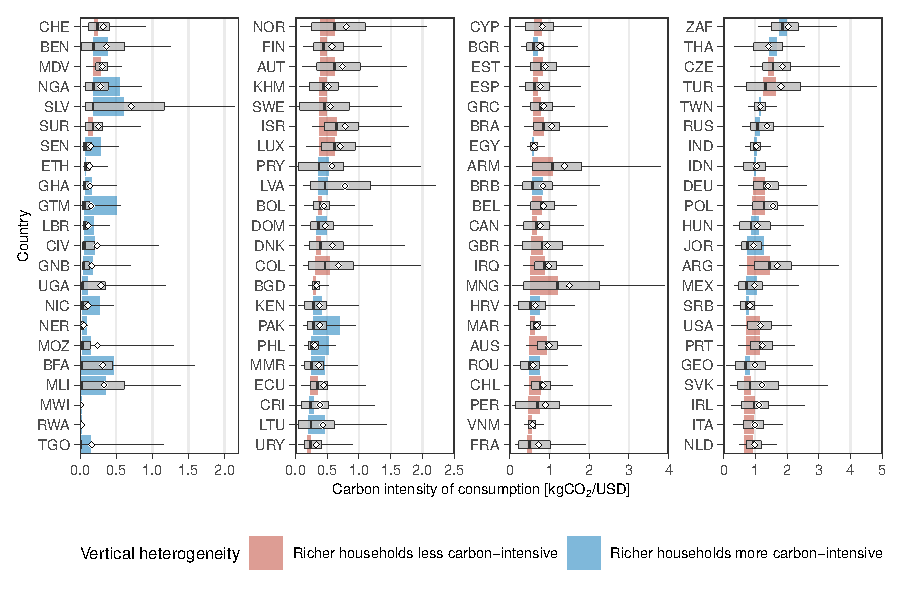
\includegraphics{1_Figures/Figures_Appendix/Figure_1_2017_Appendix_1}
  \begin{subcaption2}
    This figure displays the distribution of carbon intensity of consumption in kgCO$_{2}$/USD (x-axis) over expenditure quintiles (y-axis) for 30 countries. The first expenditure quintile comprises those 20\% of all households with least total expenditures per capita. The fifth expenditure quintile comprises those 20\% of all households with largest expenditures per capita. Within quintiles, boxes display the 25$^{th}$ and the 75$^{th}$ percentile; whiskers display the 5$^{th}$ and 95$^{th}$ percentile; rhombuses indicate the within-quintile average. Vertical coloured bands indicate the difference between the highest and the lowest quintile-level median carbon intensity of consumption. Blue bands indicate higher carbon intensities among richer households; red bands indicate higher carbon intensities among poorer households. See also Tables \ref{tab:A3} and \ref{tab:A7}.
  \end{subcaption2}

\end{figure}

\clearpage

\begin{figure}[ht!]
  \centering
  \caption{Distribution of carbon intensities over expenditure quintiles - Part B} \label{fig:Quint_B}
  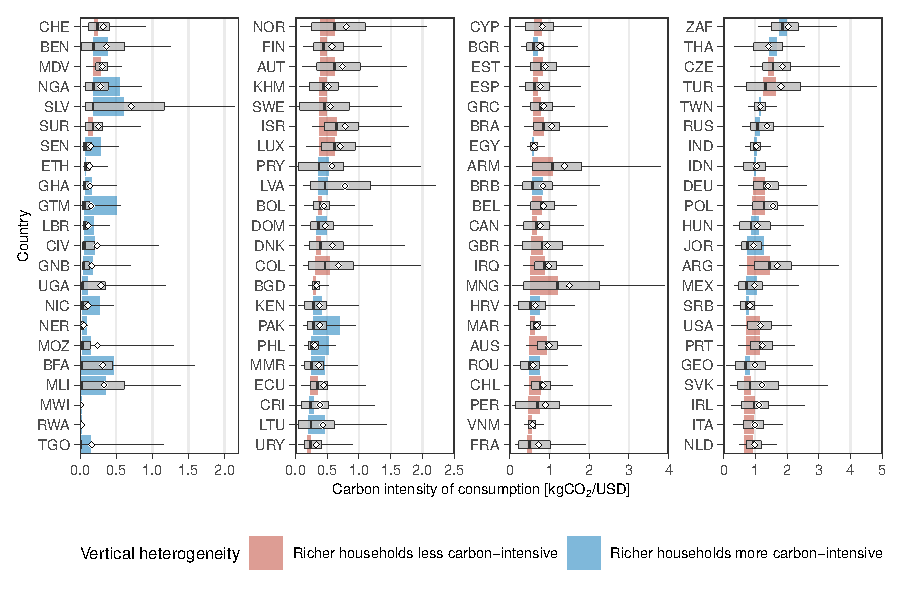
\includegraphics{1_Figures/Figures_Appendix/Figure_1_2017_Appendix_2}
  \begin{subcaption2}
    This figure displays the distribution of carbon intensity of consumption in kgCO$_{2}$/USD (x-axis) over expenditure quintiles (y-axis) for 30 countries. The first expenditure quintile comprises those 20\% of all households with least total expenditures per capita. The fifth expenditure quintile comprises those 20\% of all households with largest expenditures per capita. Within quintiles, boxes display the 25$^{th}$ and the 75$^{th}$ percentile; whiskers display the 5$^{th}$ and 95$^{th}$ percentile; rhombuses indicate the within-quintile average. Vertical coloured bands indicate the difference between the highest and the lowest quintile-level median carbon intensity of consumption. Blue bands indicate higher carbon intensities among richer households; red bands indicate higher carbon intensities among poorer households. See also Tables \ref{tab:A3} and \ref{tab:A7}.
  \end{subcaption2}

\end{figure}

\clearpage

\begin{figure}[ht!]
  \centering
  \caption{Distribution of carbon intensities over expenditure quintiles - Part C} \label{fig:Quint_C}
  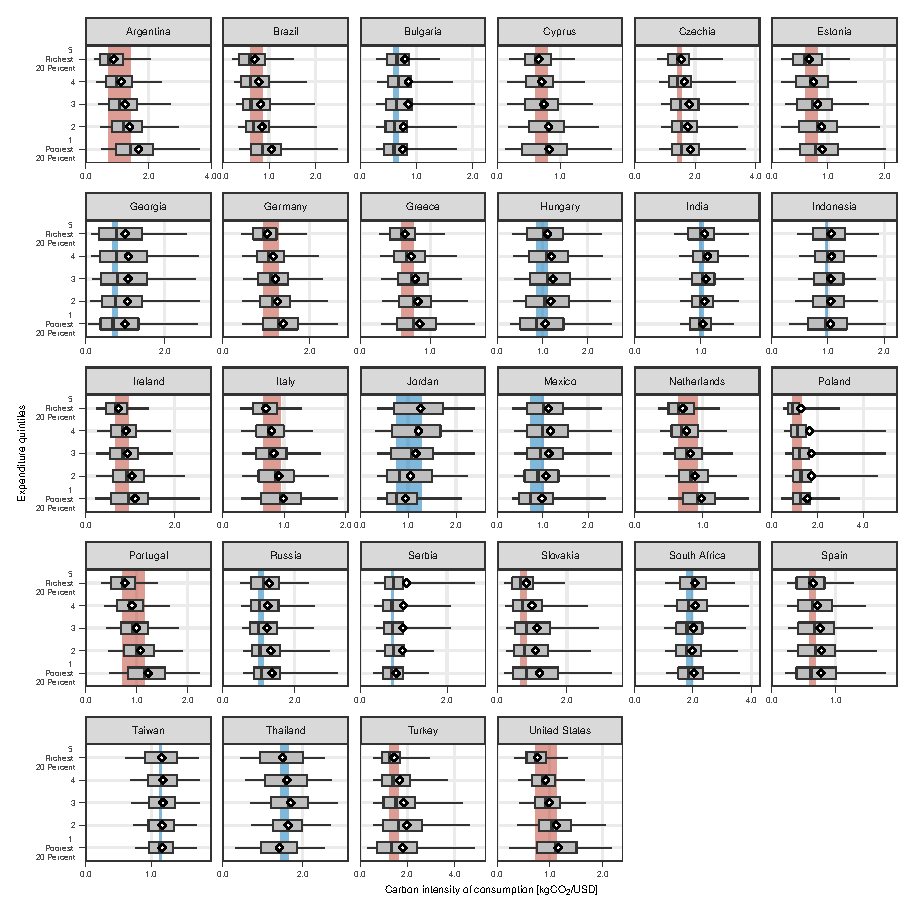
\includegraphics{1_Figures/Figures_Appendix/Figure_1_2017_Appendix_3}
  \begin{subcaption2}
    This figure displays the distribution of carbon intensity of consumption in kgCO$_{2}$/USD (x-axis) over expenditure quintiles (y-axis) for 27 countries. The first expenditure quintile comprises those 20\% of all households with least total expenditures per capita. The fifth expenditure quintile comprises those 20\% of all households with largest expenditures per capita. Within quintiles, boxes display the 25$^{th}$ and the 75$^{th}$ percentile; whiskers display the 5$^{th}$ and 95$^{th}$ percentile; rhombuses indicate the within-quintile average. Vertical coloured bands indicate the difference between the highest and the lowest quintile-level median carbon intensity of consumption. Blue bands indicate higher carbon intensities among richer households; red bands indicate higher carbon intensities among poorer households. See also Tables \ref{tab:A3} and \ref{tab:A7}.
  \end{subcaption2}

\end{figure}

\clearpage

% Carbon intensity of consumption over total household expenditures

% \begin{figure}[ht!]
%   \centering
%   \caption{Carbon intensity of consumption over total household expenditures - Part A} \label{fig:C1}
%   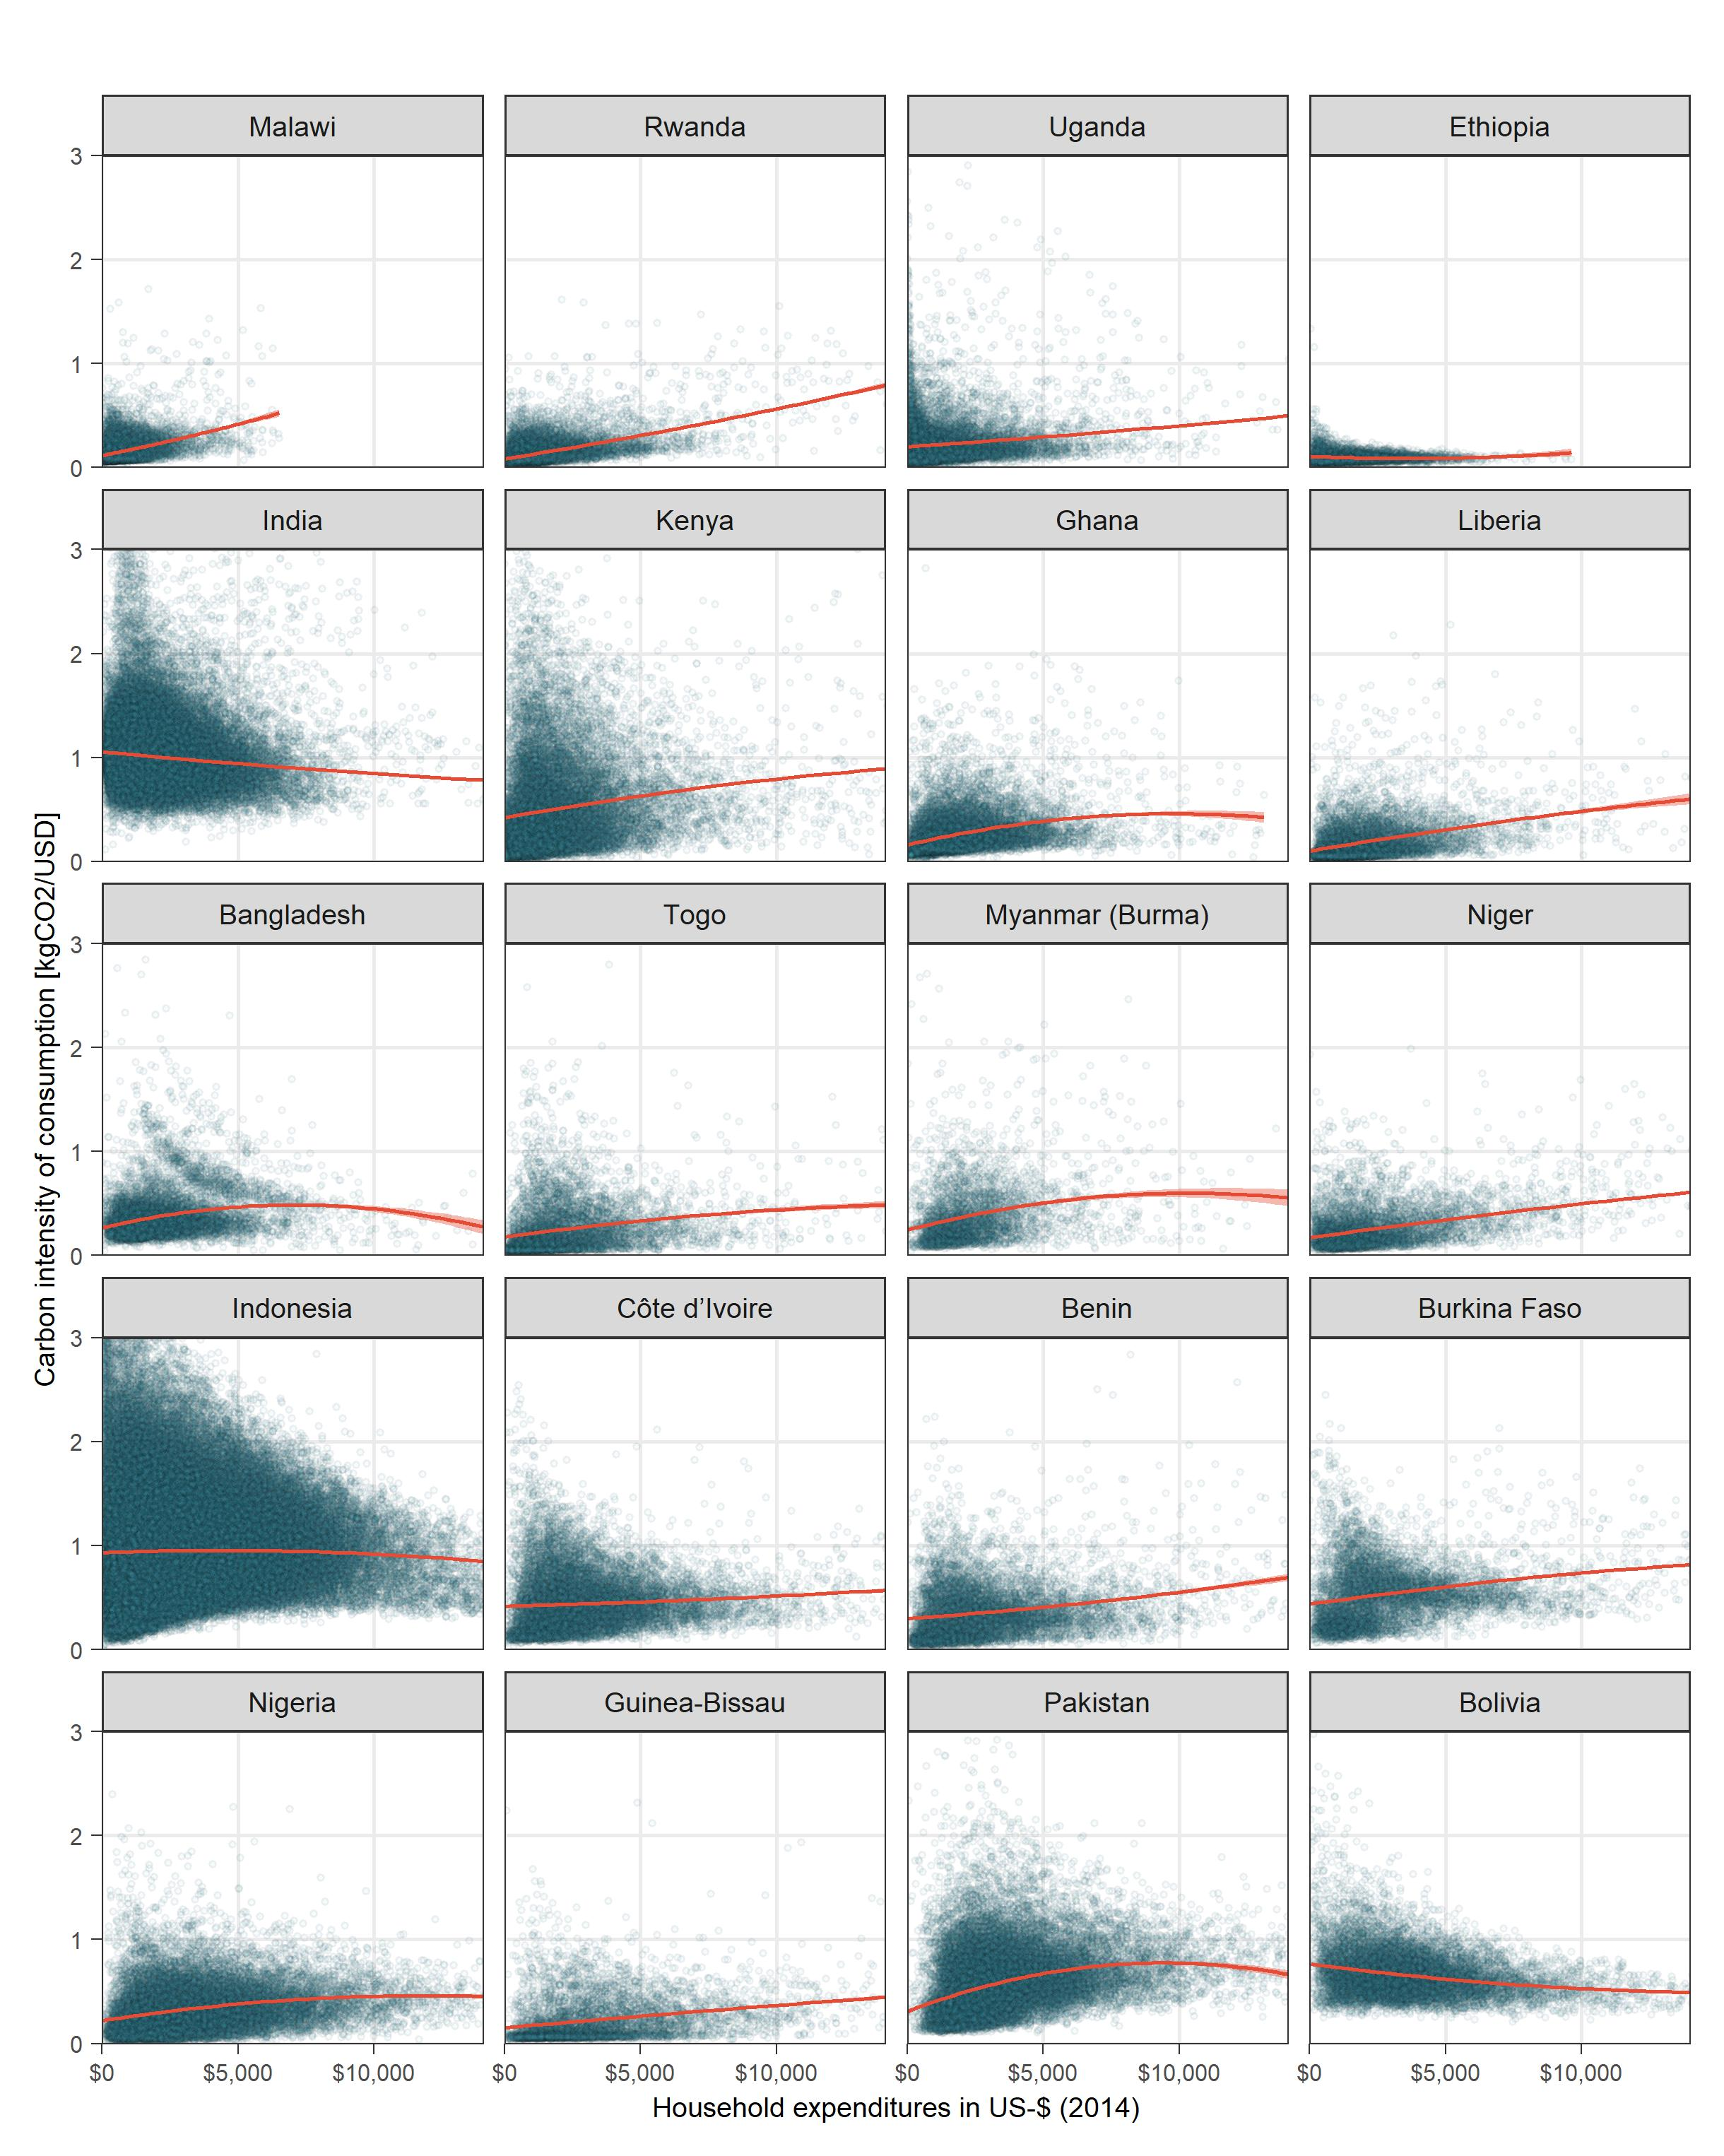
\includegraphics{Analysis_Carbon_Intensity_Curve/All_Panel_A}
%   \begin{subcaption2}
%     This figure displays carbon intensity of aggregate consumption (in $kgCO_{2}/USD$) over total household expenditures in USD for 20 countries in our sample. Household expenditures are inflated (or deflated) to 2014. Points represent single households. The red line represents a fitted curve for a quadratic OLS-regression including a 95\%-confidence interval.
%   \end{subcaption2}

% \end{figure}

% \clearpage

% \begin{figure}[ht!]
%   \centering
%  \caption{Average marginal effects of car ownership} \label{fig:D1_Car}
%   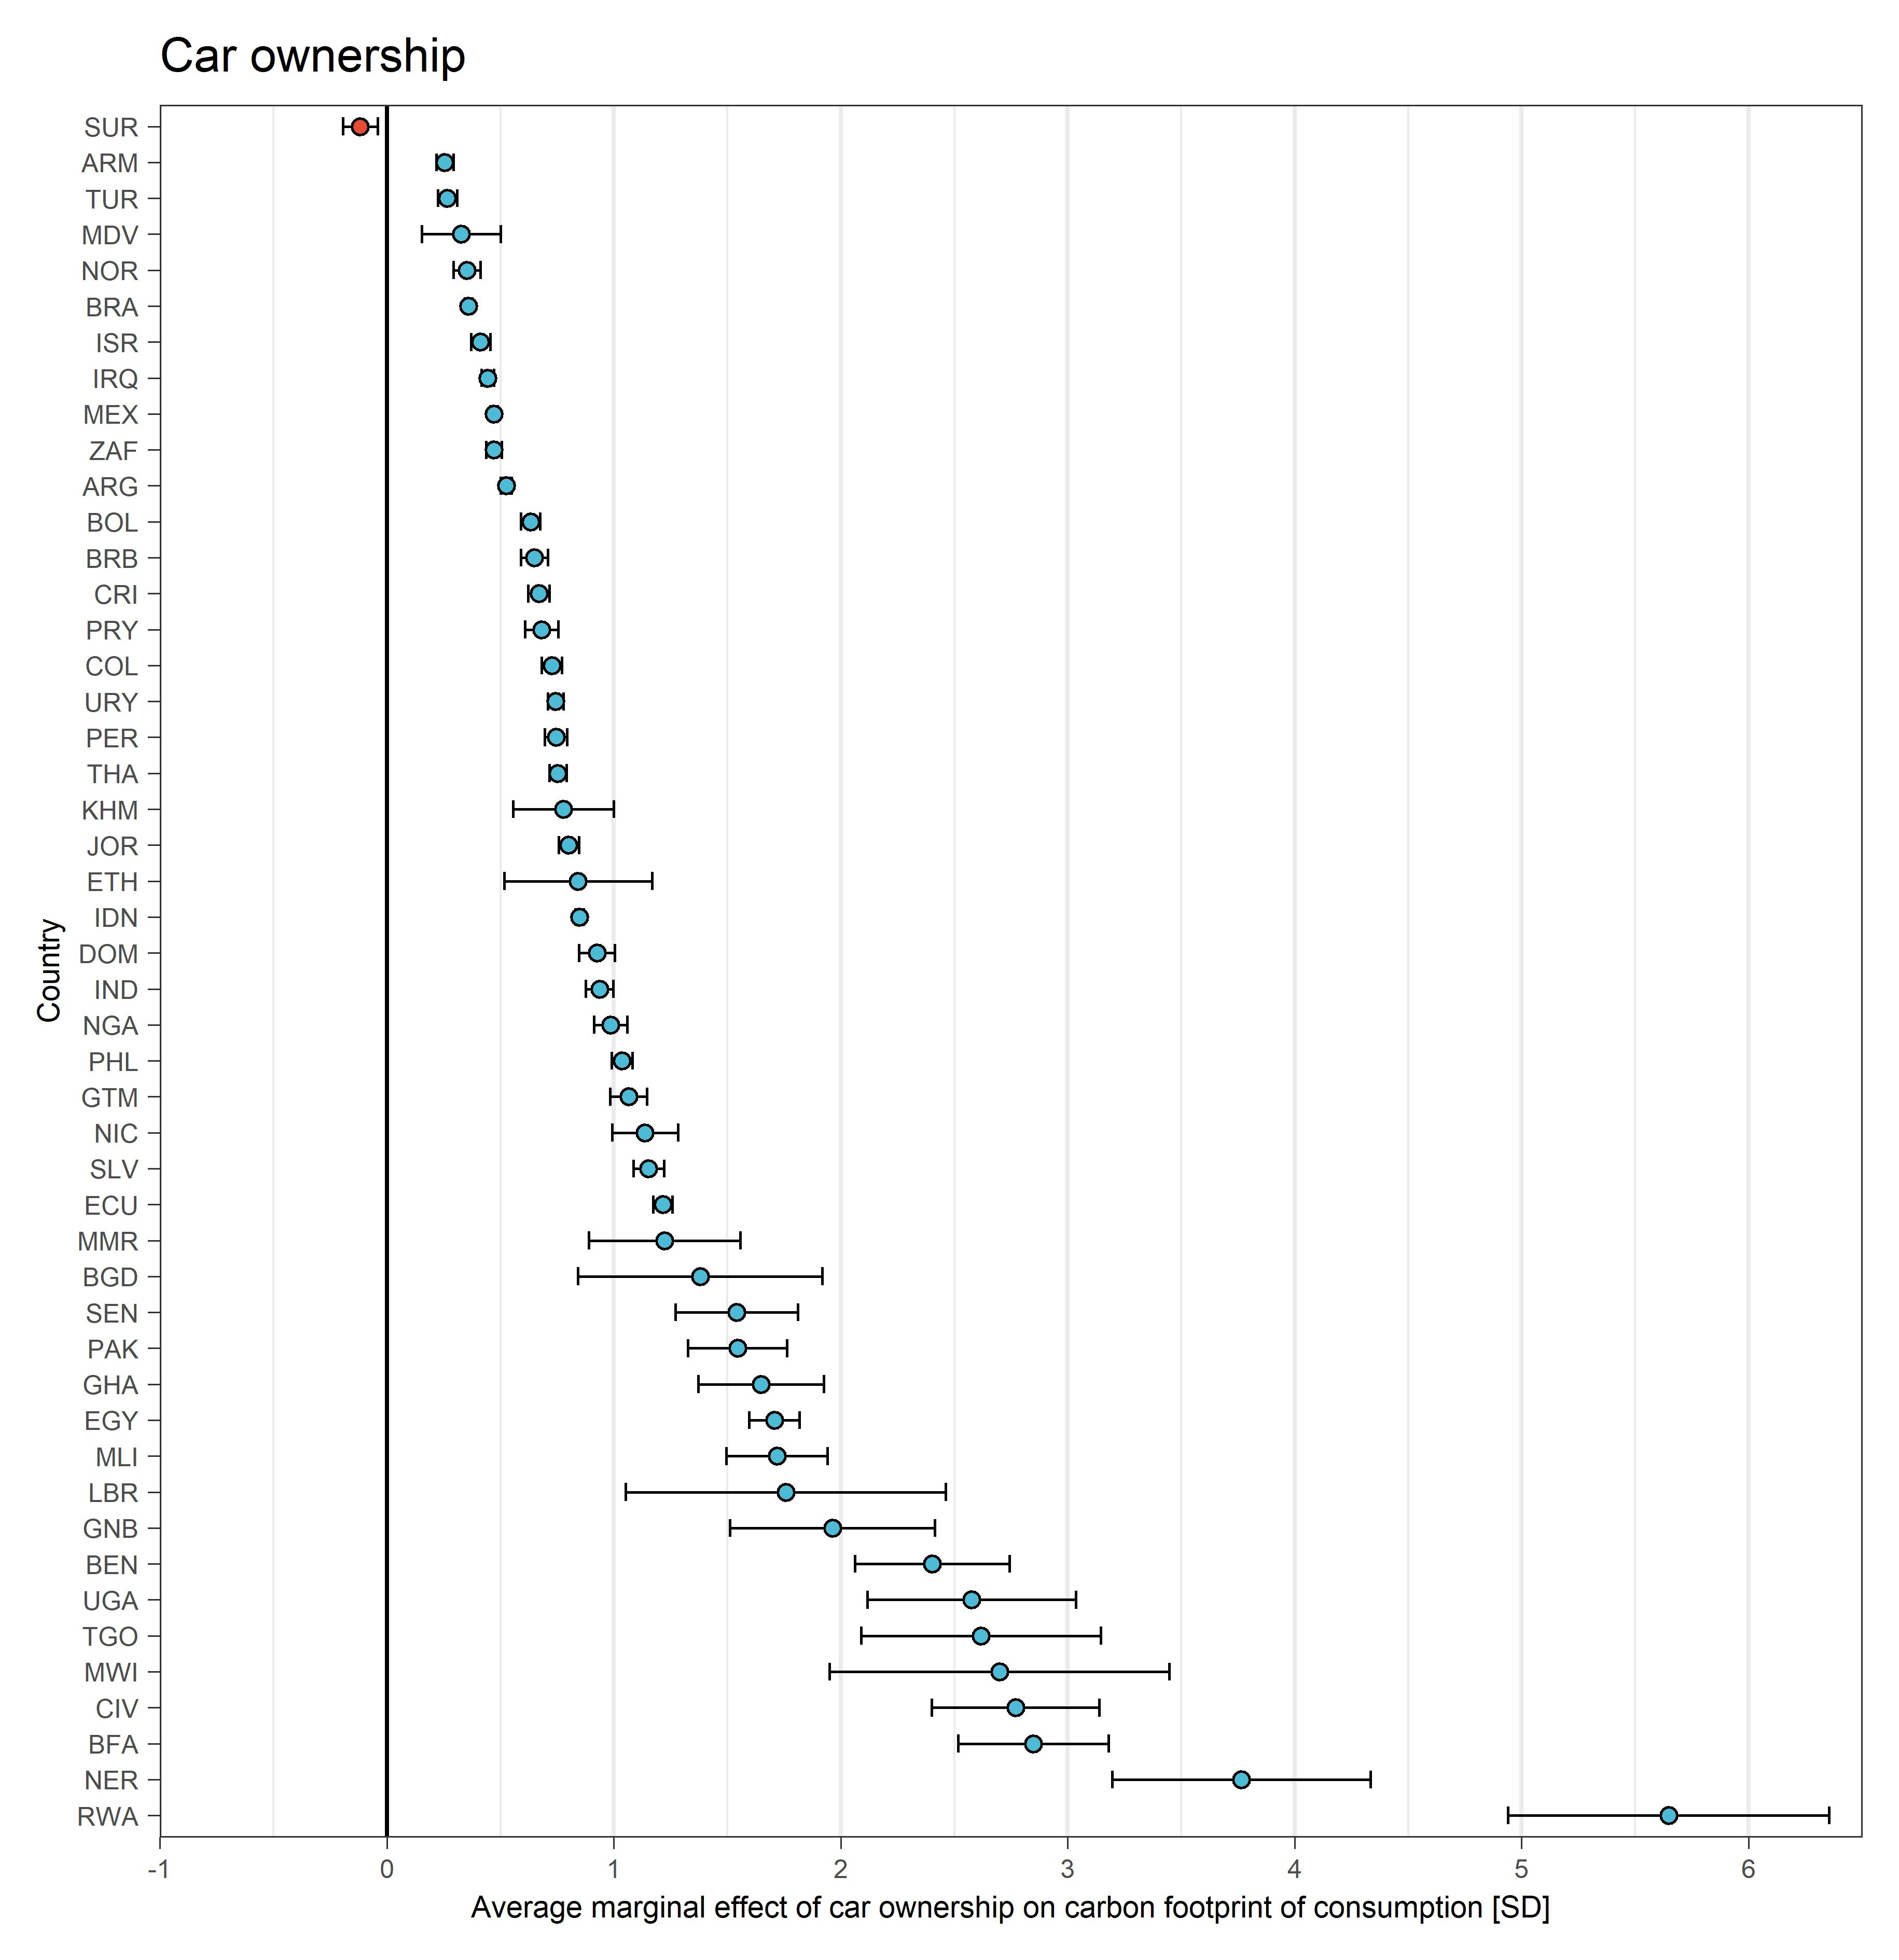
\includegraphics{Analysis_OLS_ME_Carbon_Footprint/AME_OLS_FP_car.01}
%   \begin{subcaption2}
%     This figure displays ...
%   \end{subcaption2}

% \end{figure}

% \clearpage

% \clearpage

% \begin{figure}[ht!]
%   \centering
%  \caption{Average marginal effects of cooking fuel choice - Part A} \label{fig:D6_Electricity_A}
%   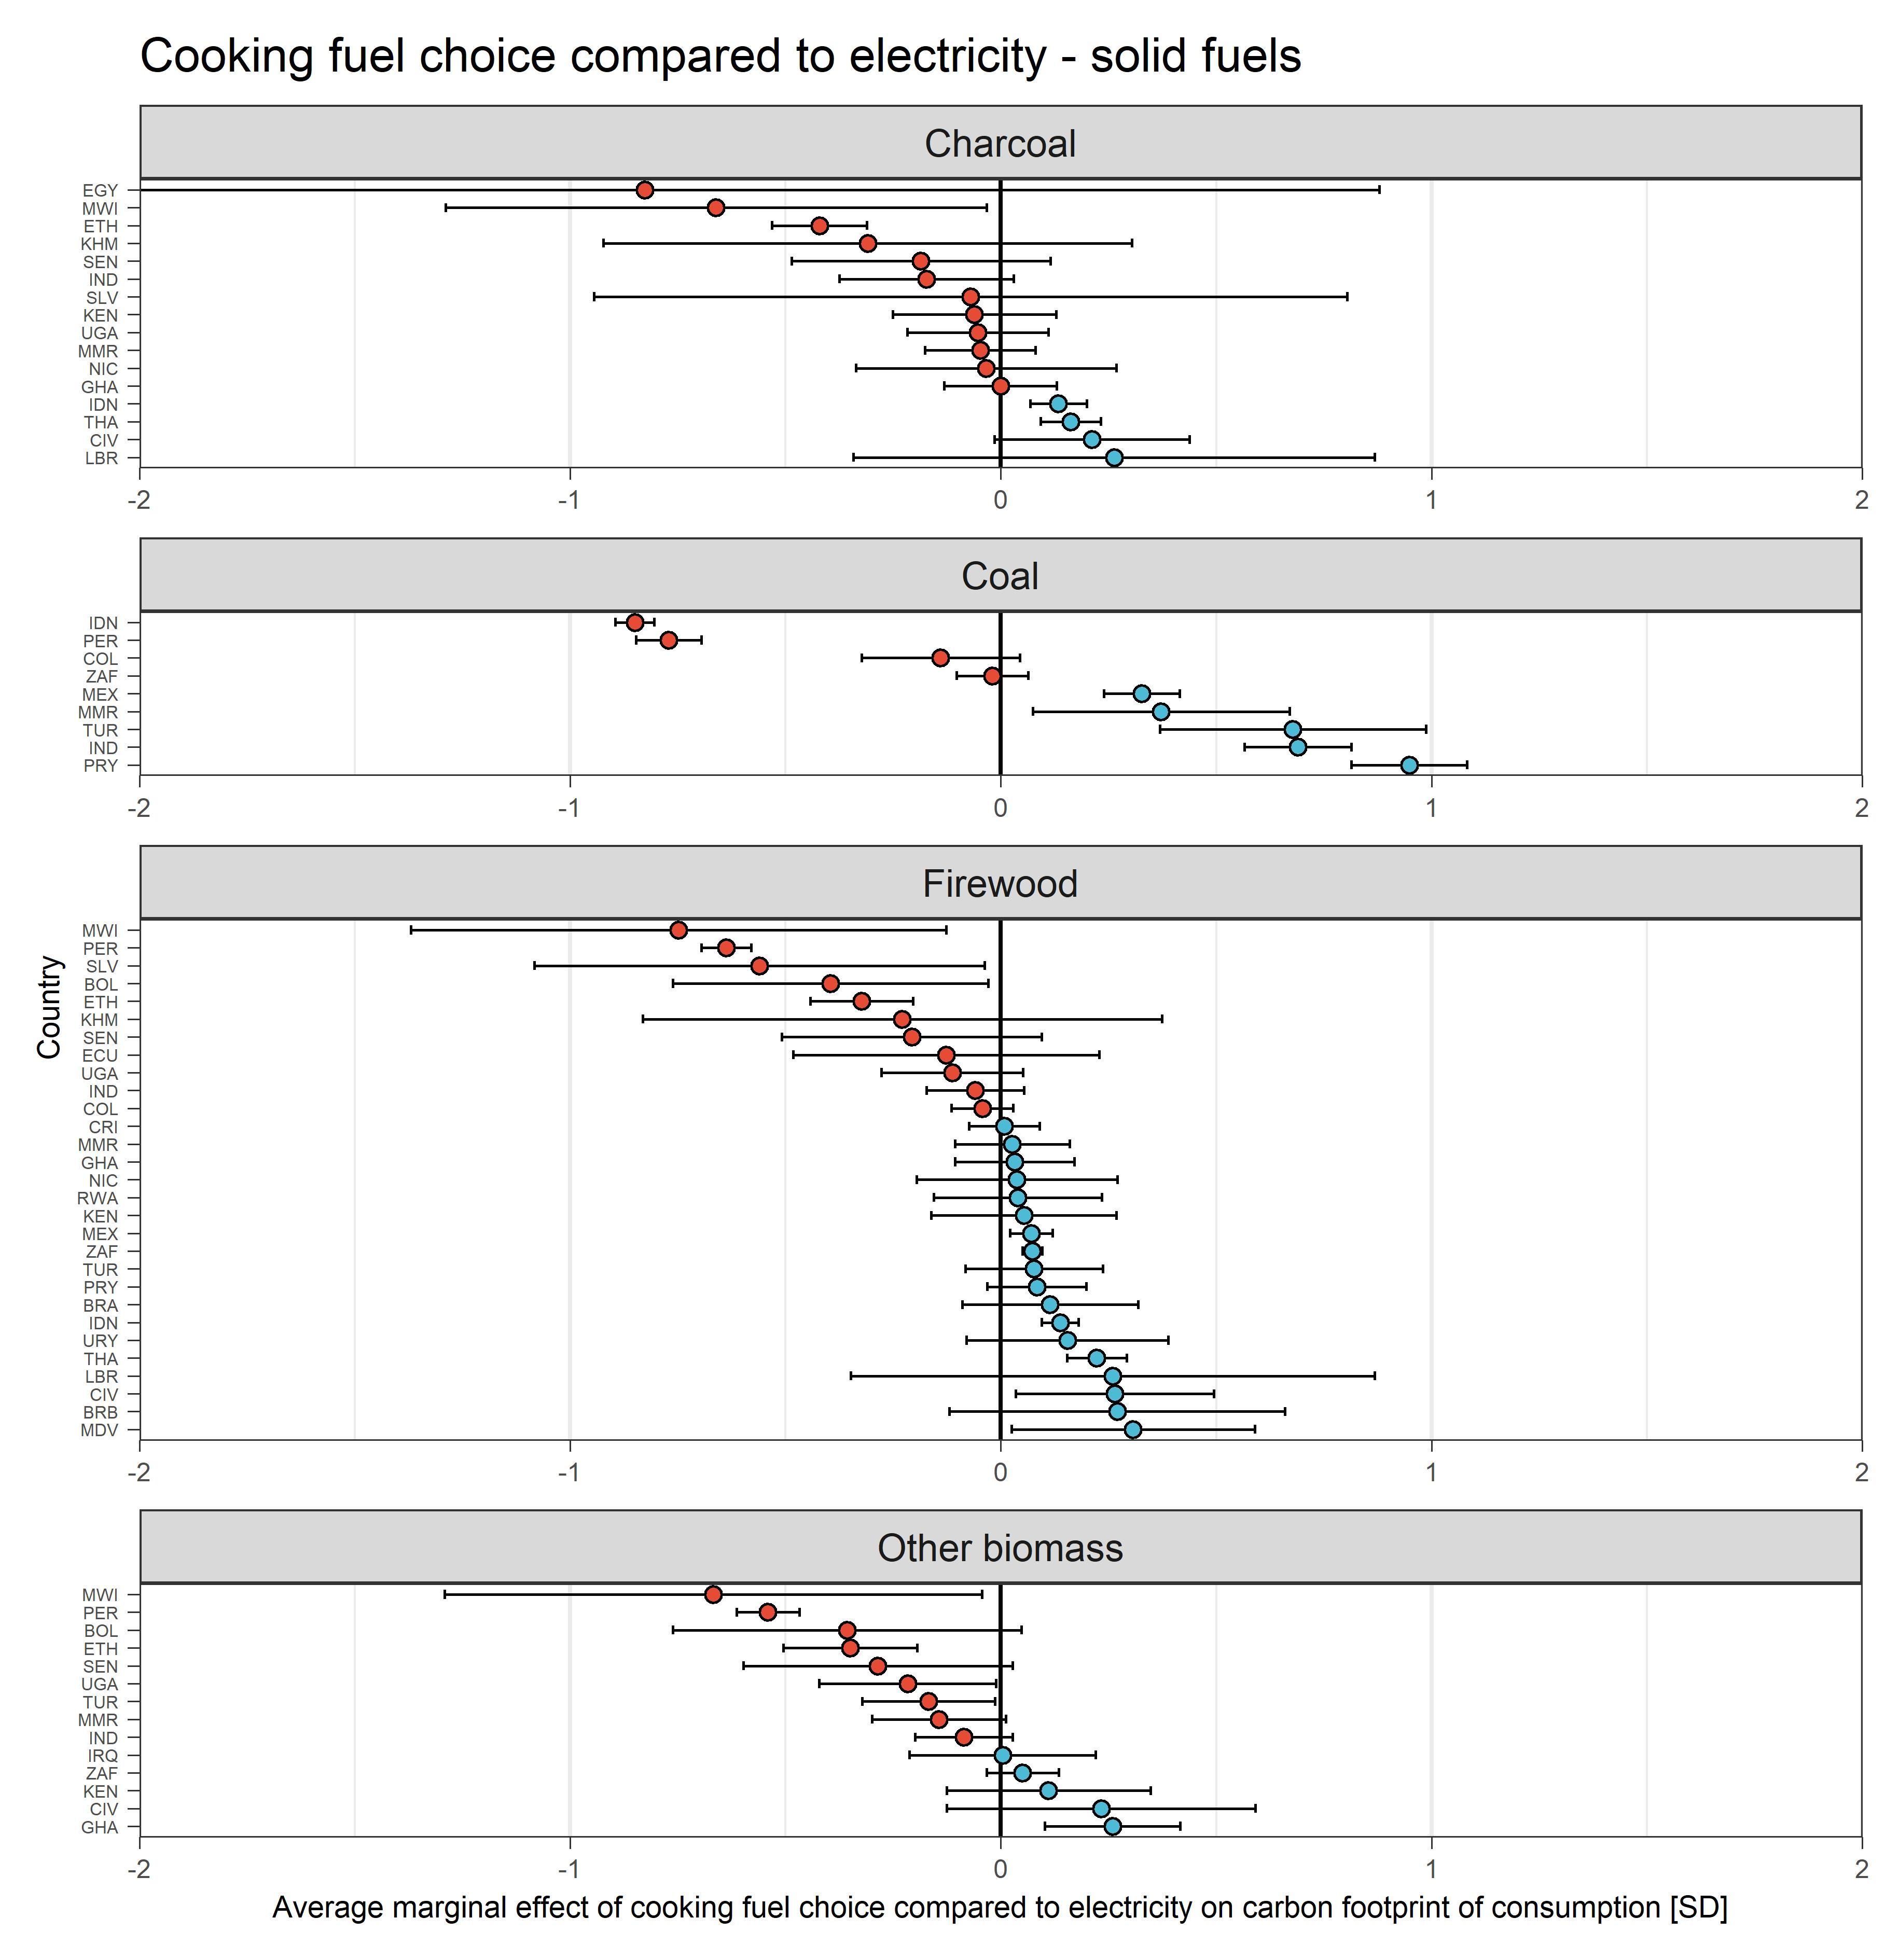
\includegraphics{Analysis_OLS_ME_Carbon_Footprint/AME_OLS_FP_CF_Electricity A}
%   \begin{subcaption2}
%     This figure displays ...
%   \end{subcaption2}

% \end{figure}

% \clearpage

% \begin{figure}[ht!]
%   \centering
%  \caption{Average marginal effects of car ownership} \label{fig:E1_Car}
%   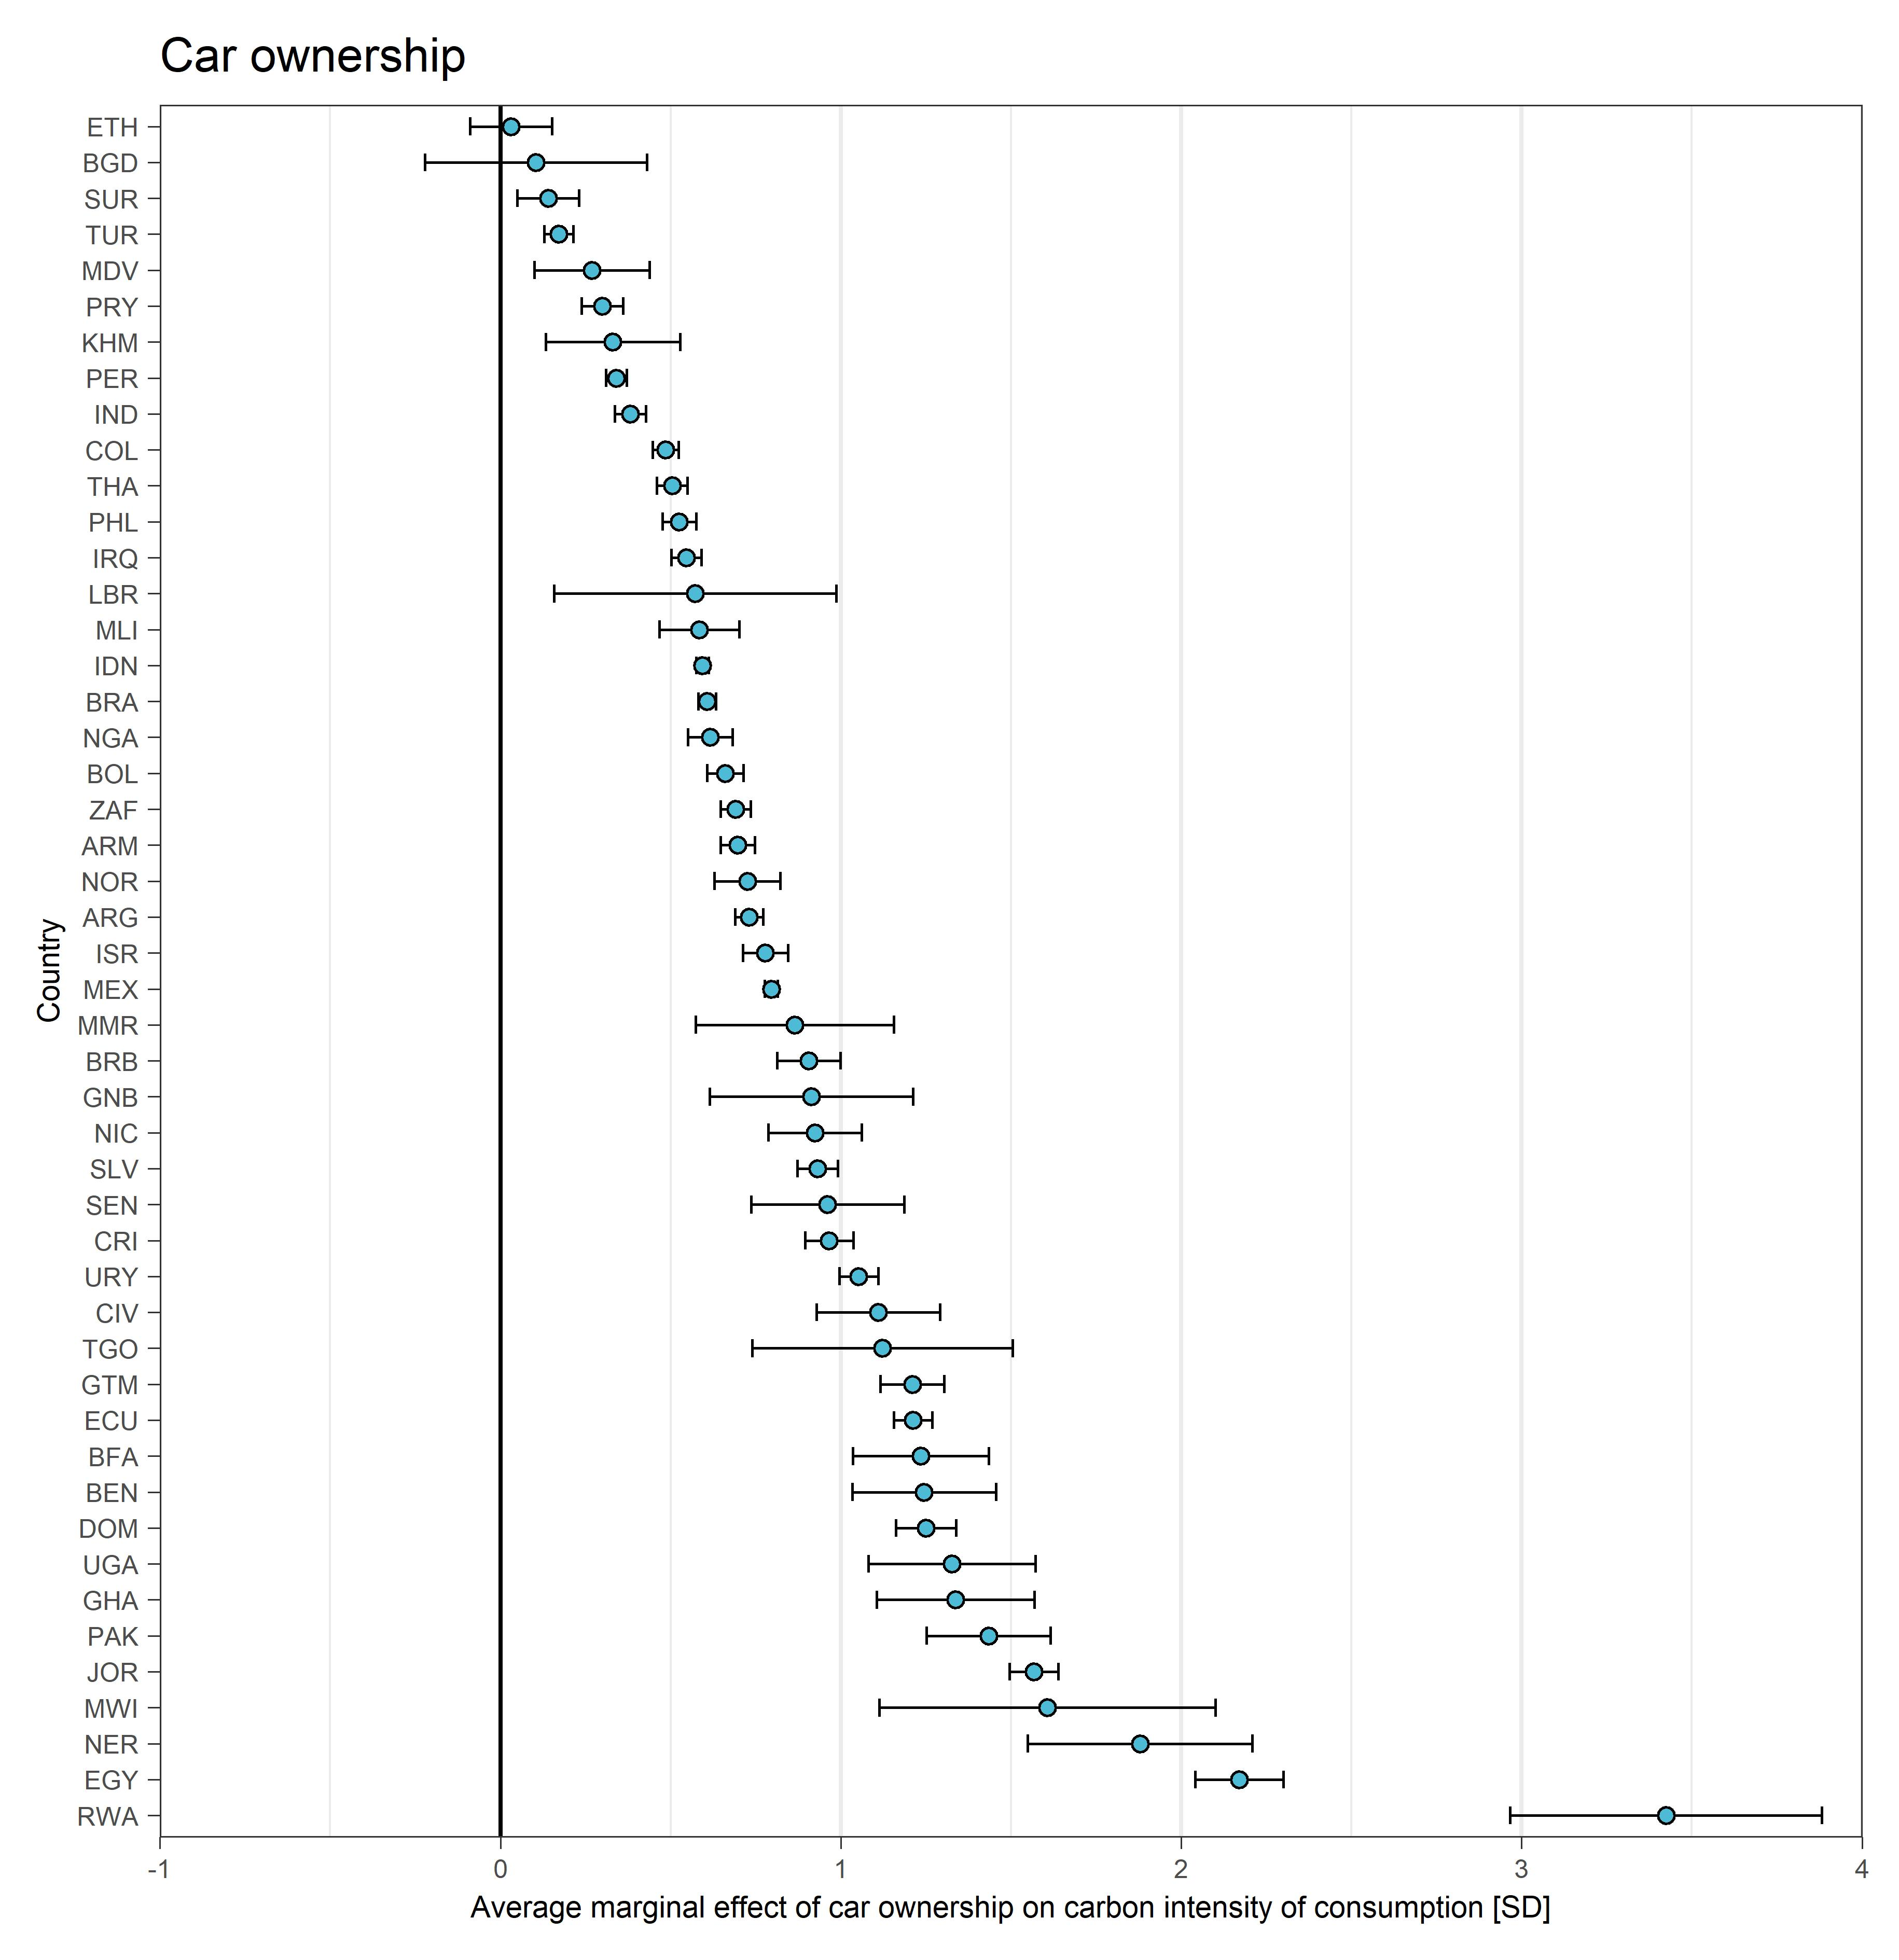
\includegraphics{Analysis_OLS_ME_Carbon_Intensity/AME_OLS_CI_car.01}
%   \begin{subcaption2}
%     This figure displays ...
%   \end{subcaption2}

% \end{figure}

% \clearpage

%  \begin{figure}[ht!]
%    \centering
%   \caption{Average marginal effects of car ownership} \label{fig:F1_Car}
%    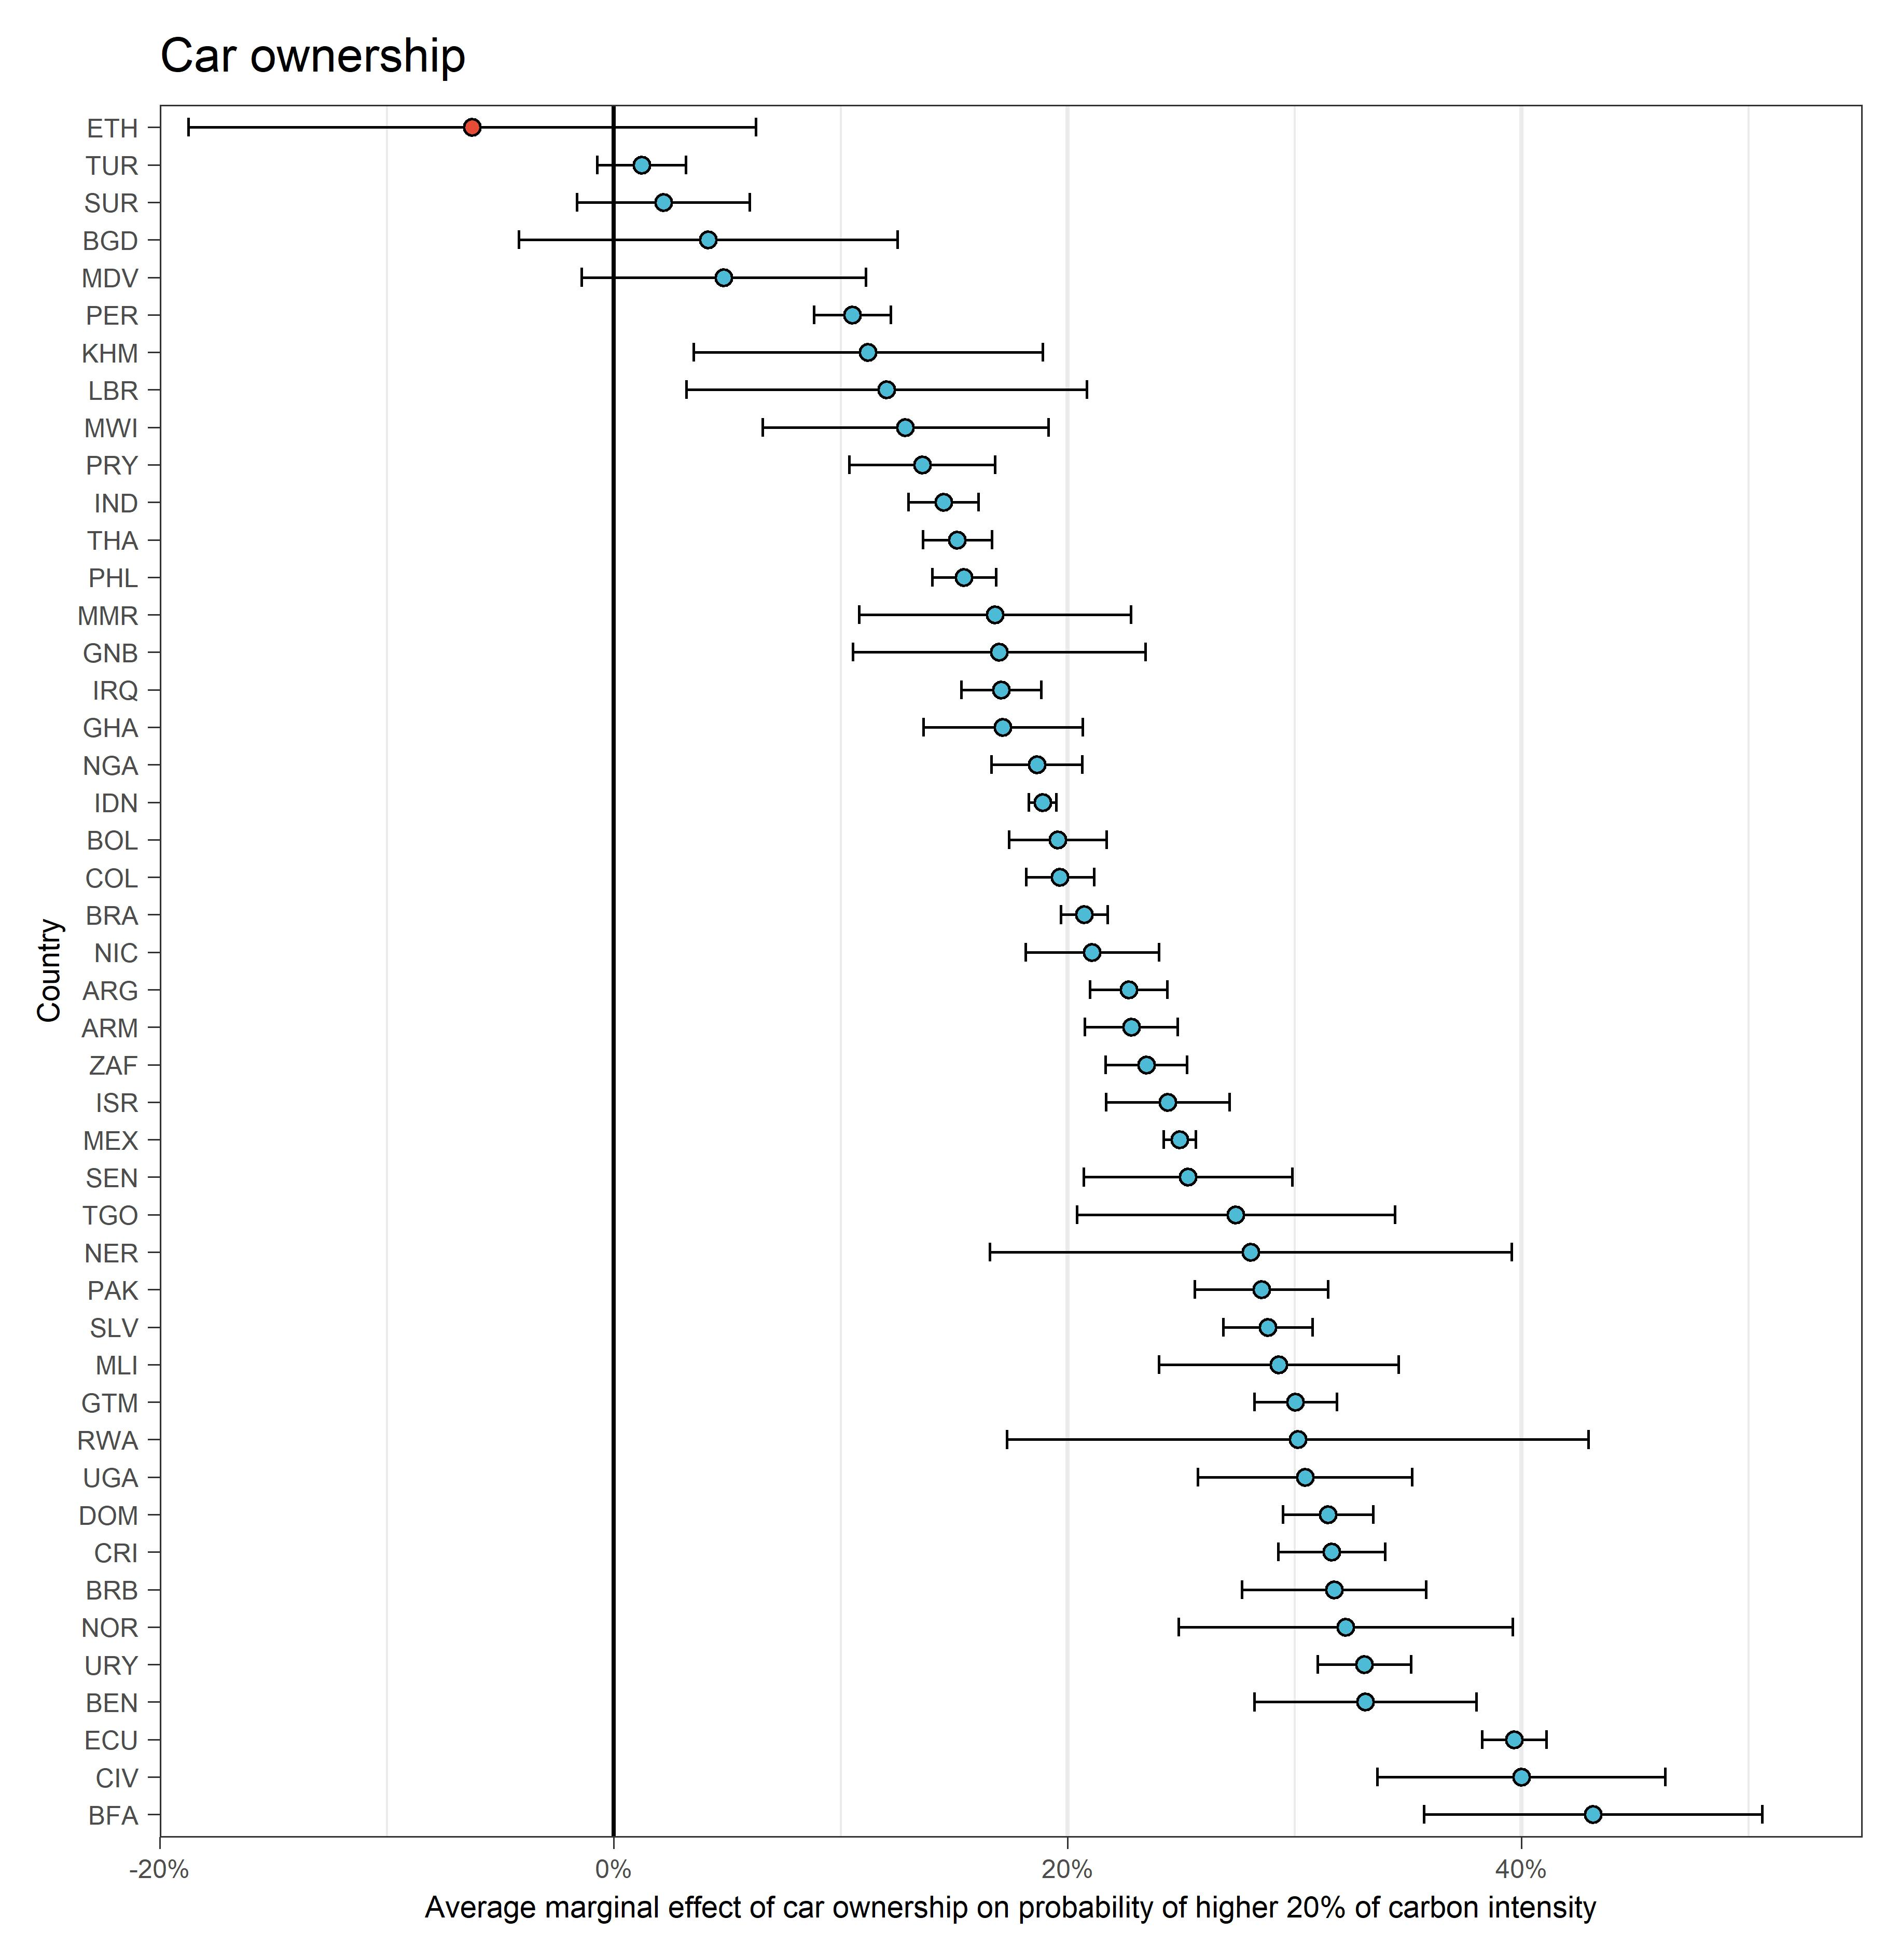
\includegraphics{Analysis_Logit_Models_Marginal_Effects/Average_Marginal_Effects_affected_upper_80_car.01}
%    \begin{subcaption2}
%      This figure displays ...
%    \end{subcaption2}

%  \end{figure}

%  \clearpage

  \begin{figure}[ht!]
   \centering
   \caption{Average silhouette width for different numbers of clusters \textit{k}} \label{fig:G3_silhouette_2}
   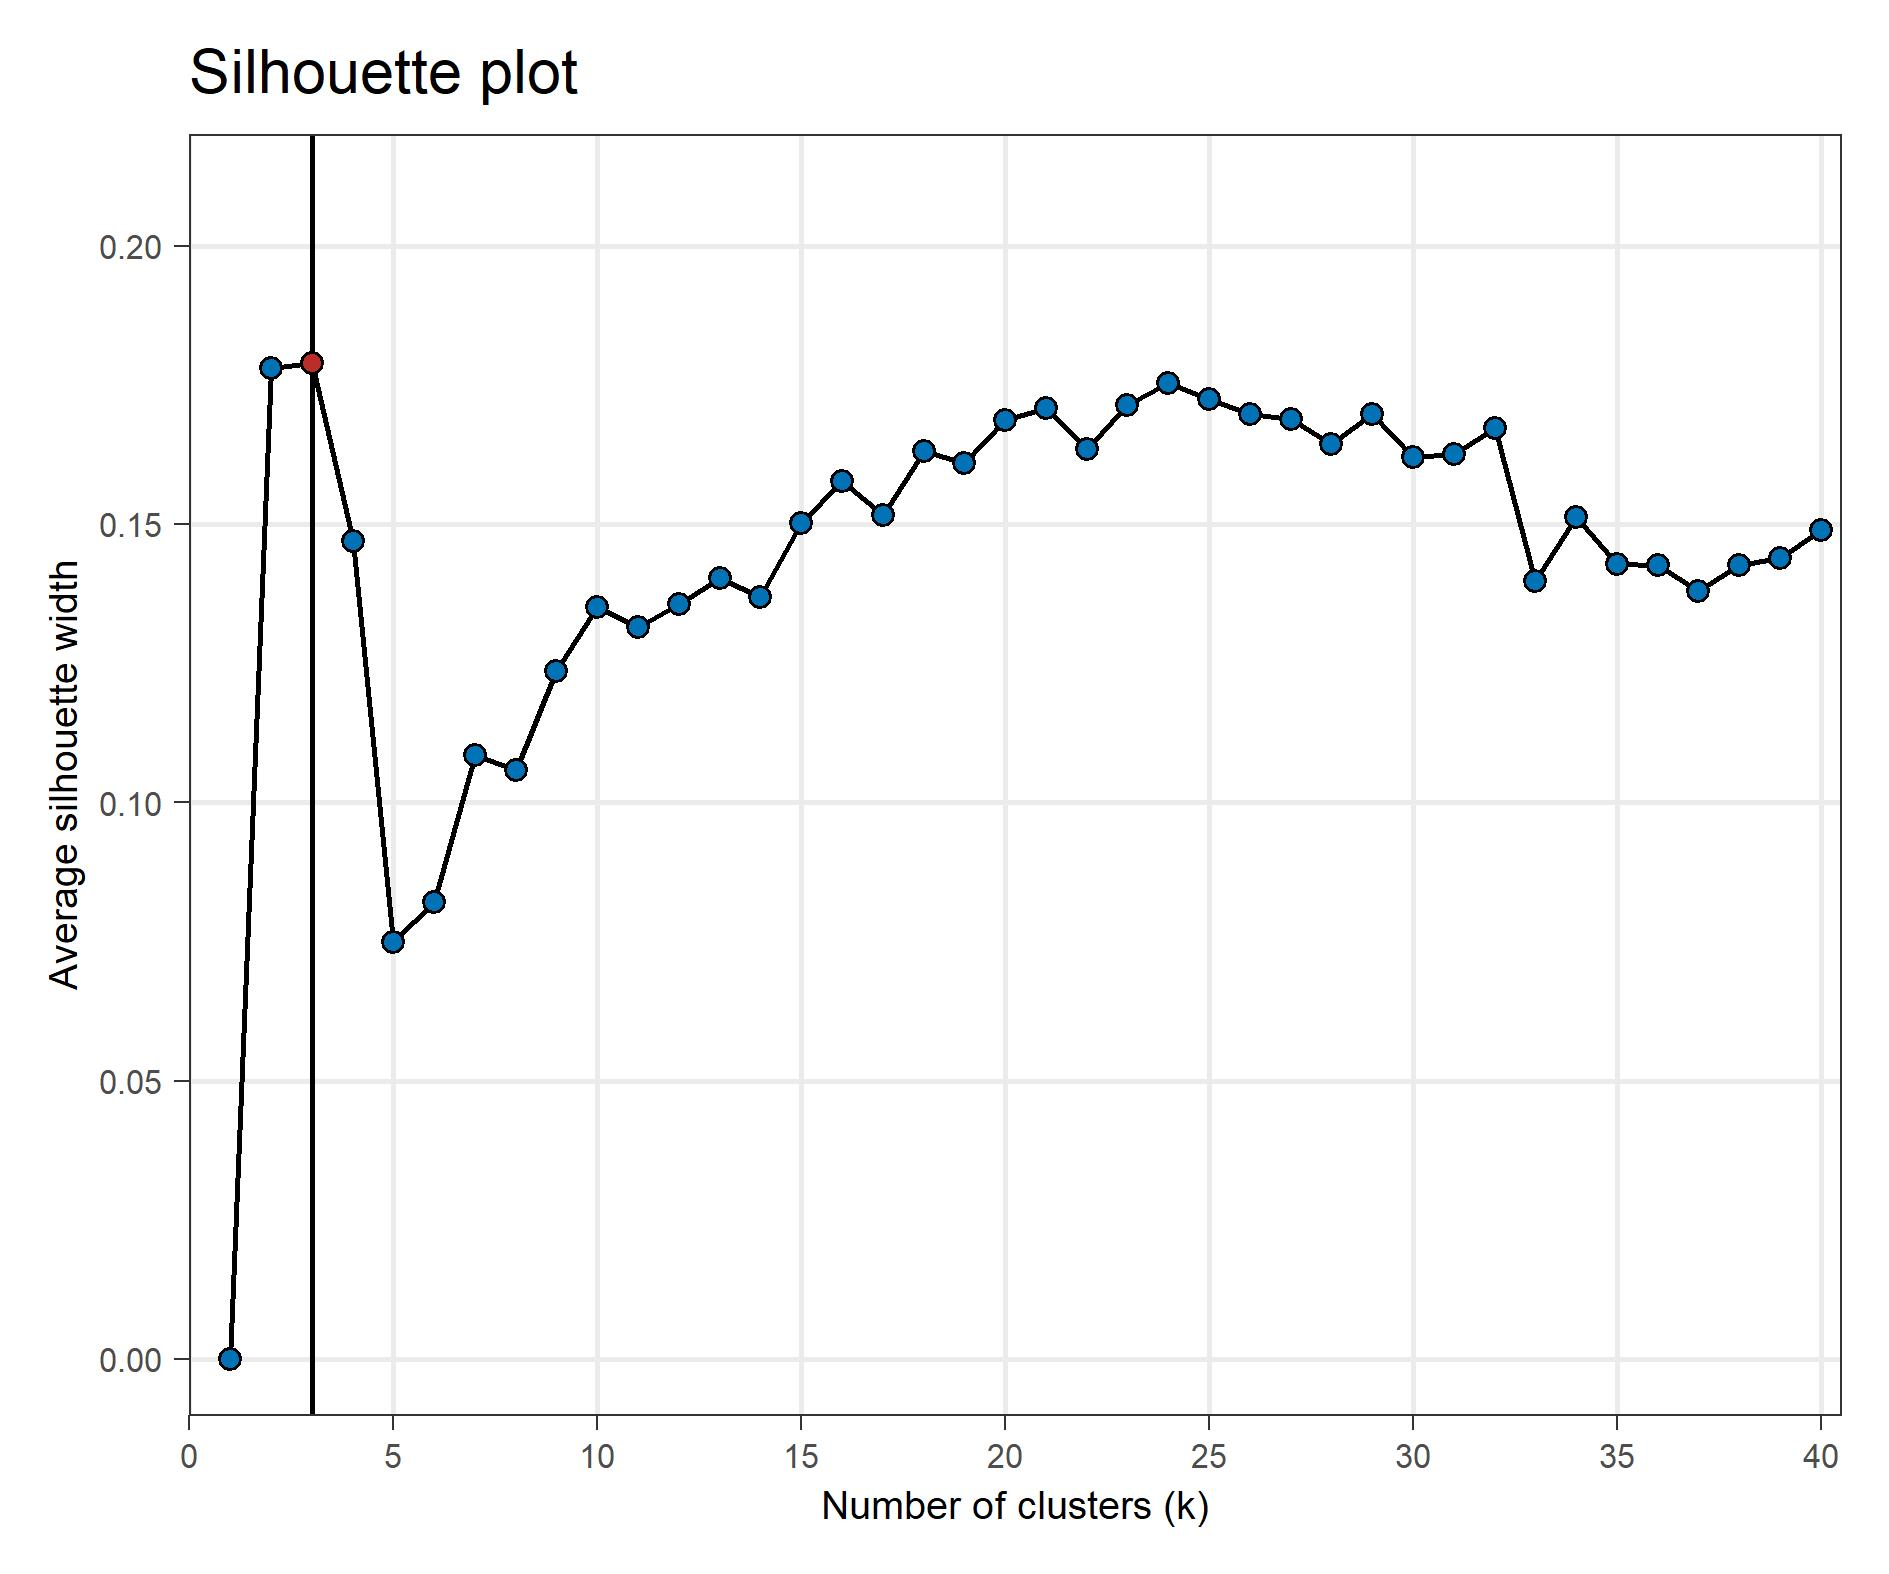
\includegraphics{Figures_Appendix/Figure_Silhouette_2}
   \begin{subcaption2}
     This figure displays the average silhouette width across all clusters for different numbers of clusters \textit{k}. We perform k-means clustering on a dataset with 87 country-level observations. Observations include information on vertical and horizontal distribution, average carbon intensity and \textit{adjusted} feature importance, i.e., we adjust feature importance for country-level model performance. Vertical line and red point indicate the number of clusters that maximizes average silhouette width across all clusters.
   \end{subcaption2}
 \end{figure}

 \clearpage

 \begin{figure}[ht!]
   \centering
   \caption{Average silhouette width for each country per cluster \textit{k}} \label{fig:G4_silhouette_2}
   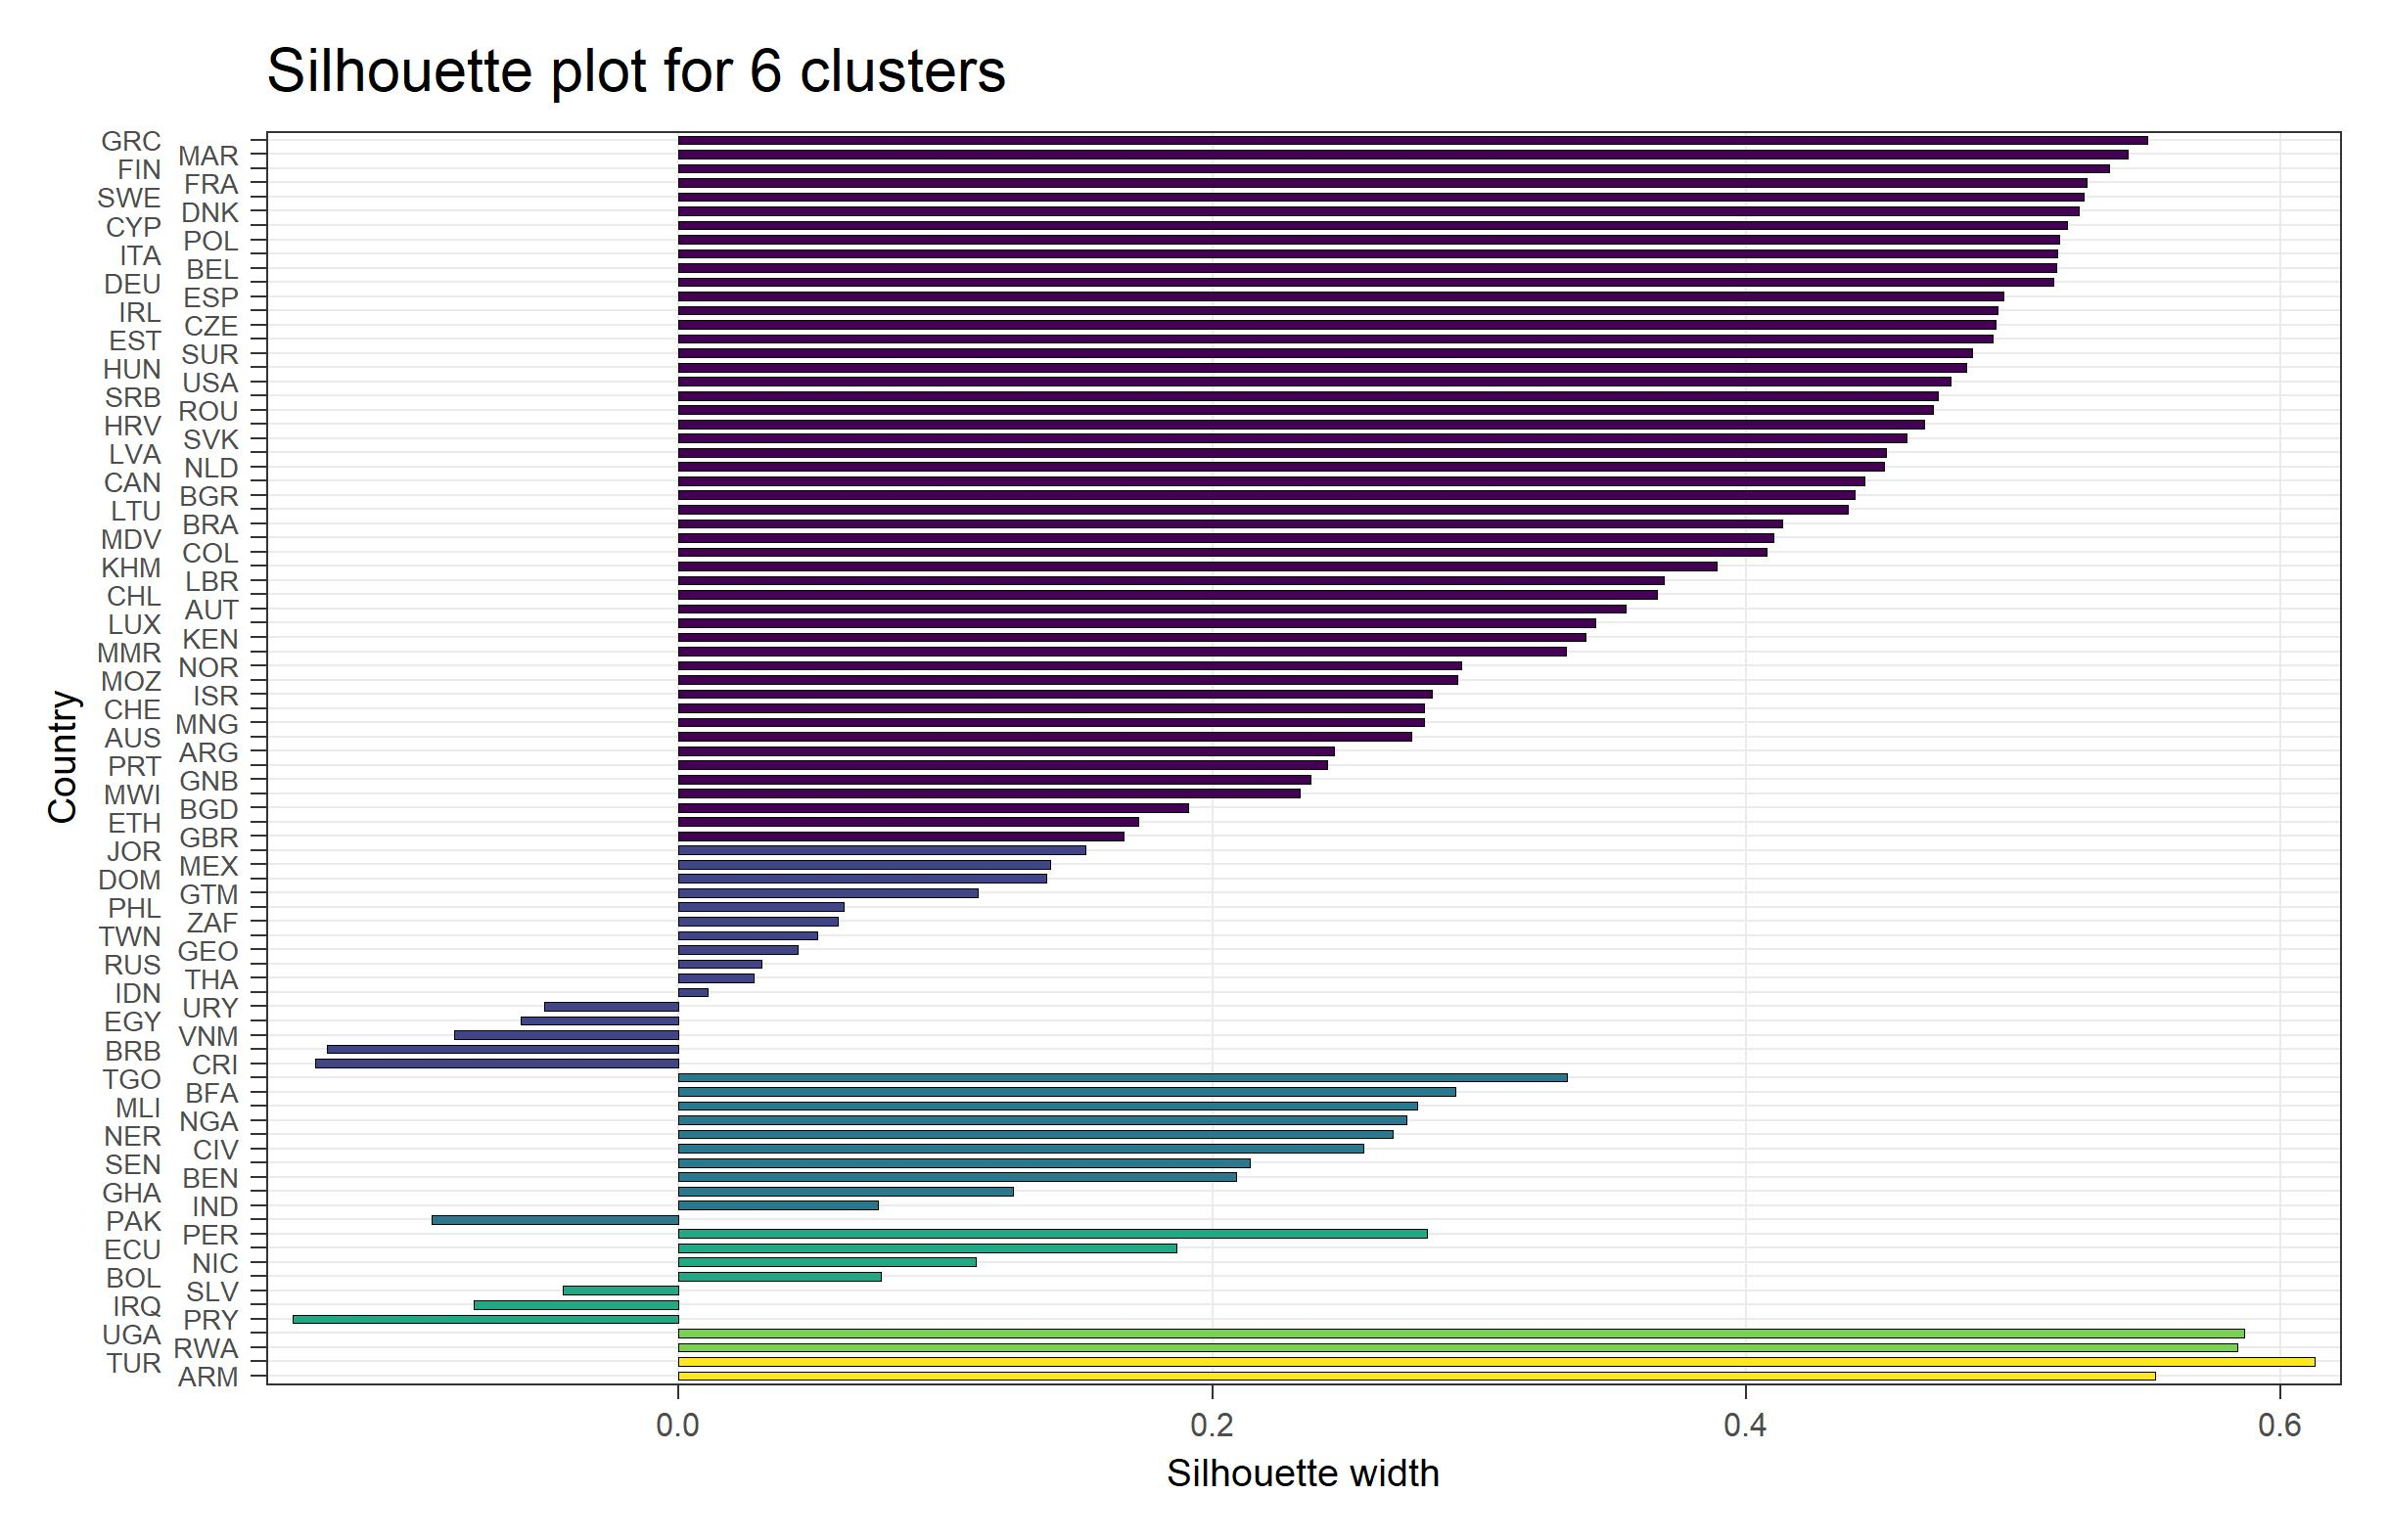
\includegraphics{Figures_Appendix/Figure_Silhouette_Clusters_2}
   \begin{subcaption2}
     This figure displays the silhouette for each country for nine clusters. We perform k-means clustering on a dataset with 87 country-level observations. Observations include information on vertical and horizontal distribution, average carbon intensity and \textit{adjusted} feature importance, i.e. we adjust feature importance for country-level model performance. We order observations (y-axis) by clusters with most observations and by silhouette width. Silhouette width expresses how well each observation fits in its cluster, also in comparison to the observations from the least distant, but different cluster.
   \end{subcaption2}
 \end{figure}

 \clearpage

\begin{figure}[ht!]
   \centering
   \caption{Average silhouette width for different numbers of clusters \textit{k}} \label{fig:G1_silhouette}
   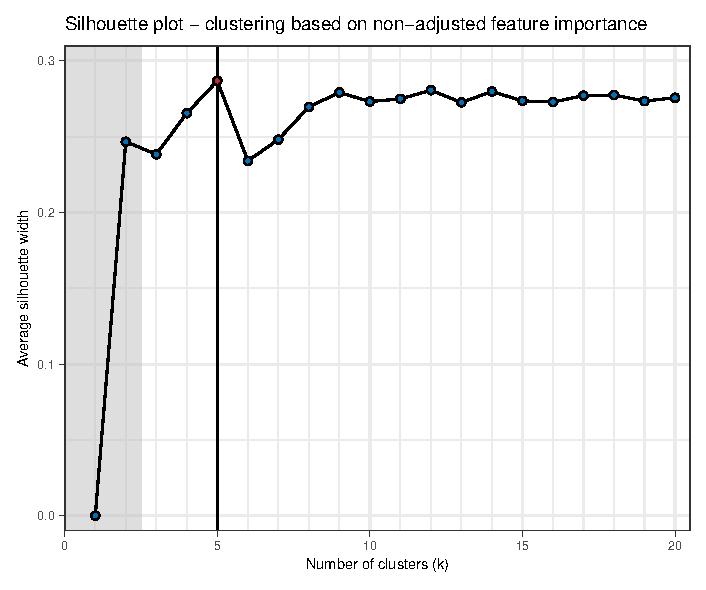
\includegraphics{Figures_Appendix/Figure_Silhouette_1}
   \begin{subcaption2}
     This figure displays the average silhouette width across all clusters for different numbers of clusters \textit{k}. We perform k-means clustering on a dataset with 87 country-level observations. Observations include information on vertical and horizontal distribution, average carbon intensity and feature importance. In contrast to Figure \ref{fig:G3_silhouette_2}, we do not adjust feature importance for country-level model performance. Vertical line and red point indicate the number of clusters that maximizes average silhouette width across all clusters.
   \end{subcaption2}
 \end{figure}

 \clearpage

 \begin{figure}[ht!]
   \centering
   \caption{Average silhouette width for each country per cluster \textit{k}} \label{fig:G2_silhouette}
   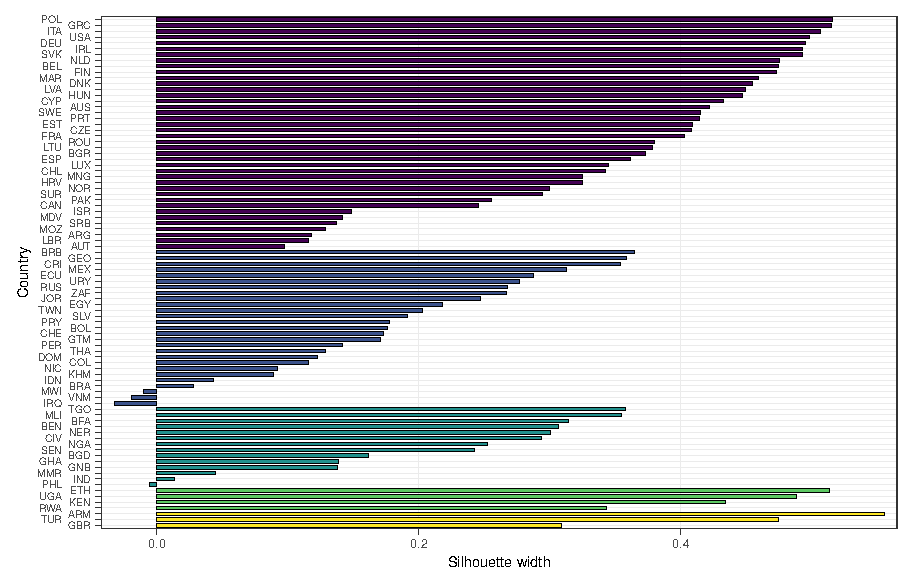
\includegraphics{Figures_Appendix/Figure_Silhouette_Clusters_1}
   \begin{subcaption2}
     This figure displays the silhouette for each country for 15 clusters. We perform k-means clustering on a dataset with 15 country-level observations. Observations include information on vertical and horizontal distribution, average carbon intensity and feature importance. In contrast to Figure \ref{fig:G2_silhouette}, we do not adjust feature importance for country-level model performance. We order observations (y-axis) by clusters with most observations and by silhouette width. Silhouette width expresses how well each observation fits in its cluster, also in comparison to the observations from the least distant, but different cluster.
   \end{subcaption2}
 \end{figure}

 \clearpage

\begin{figure}[ht!]
     \centering
    \caption{Partial dependence plot (SHAP) for 88 countries and nine clusters}
    \label{fig:5b}
     \begin{subfigure}[b]{\textwidth}
         \centering
         \caption{Partial dependence plot (SHAP) for Argentina (cluster A)}
         \label{fig:5b_ARG}
         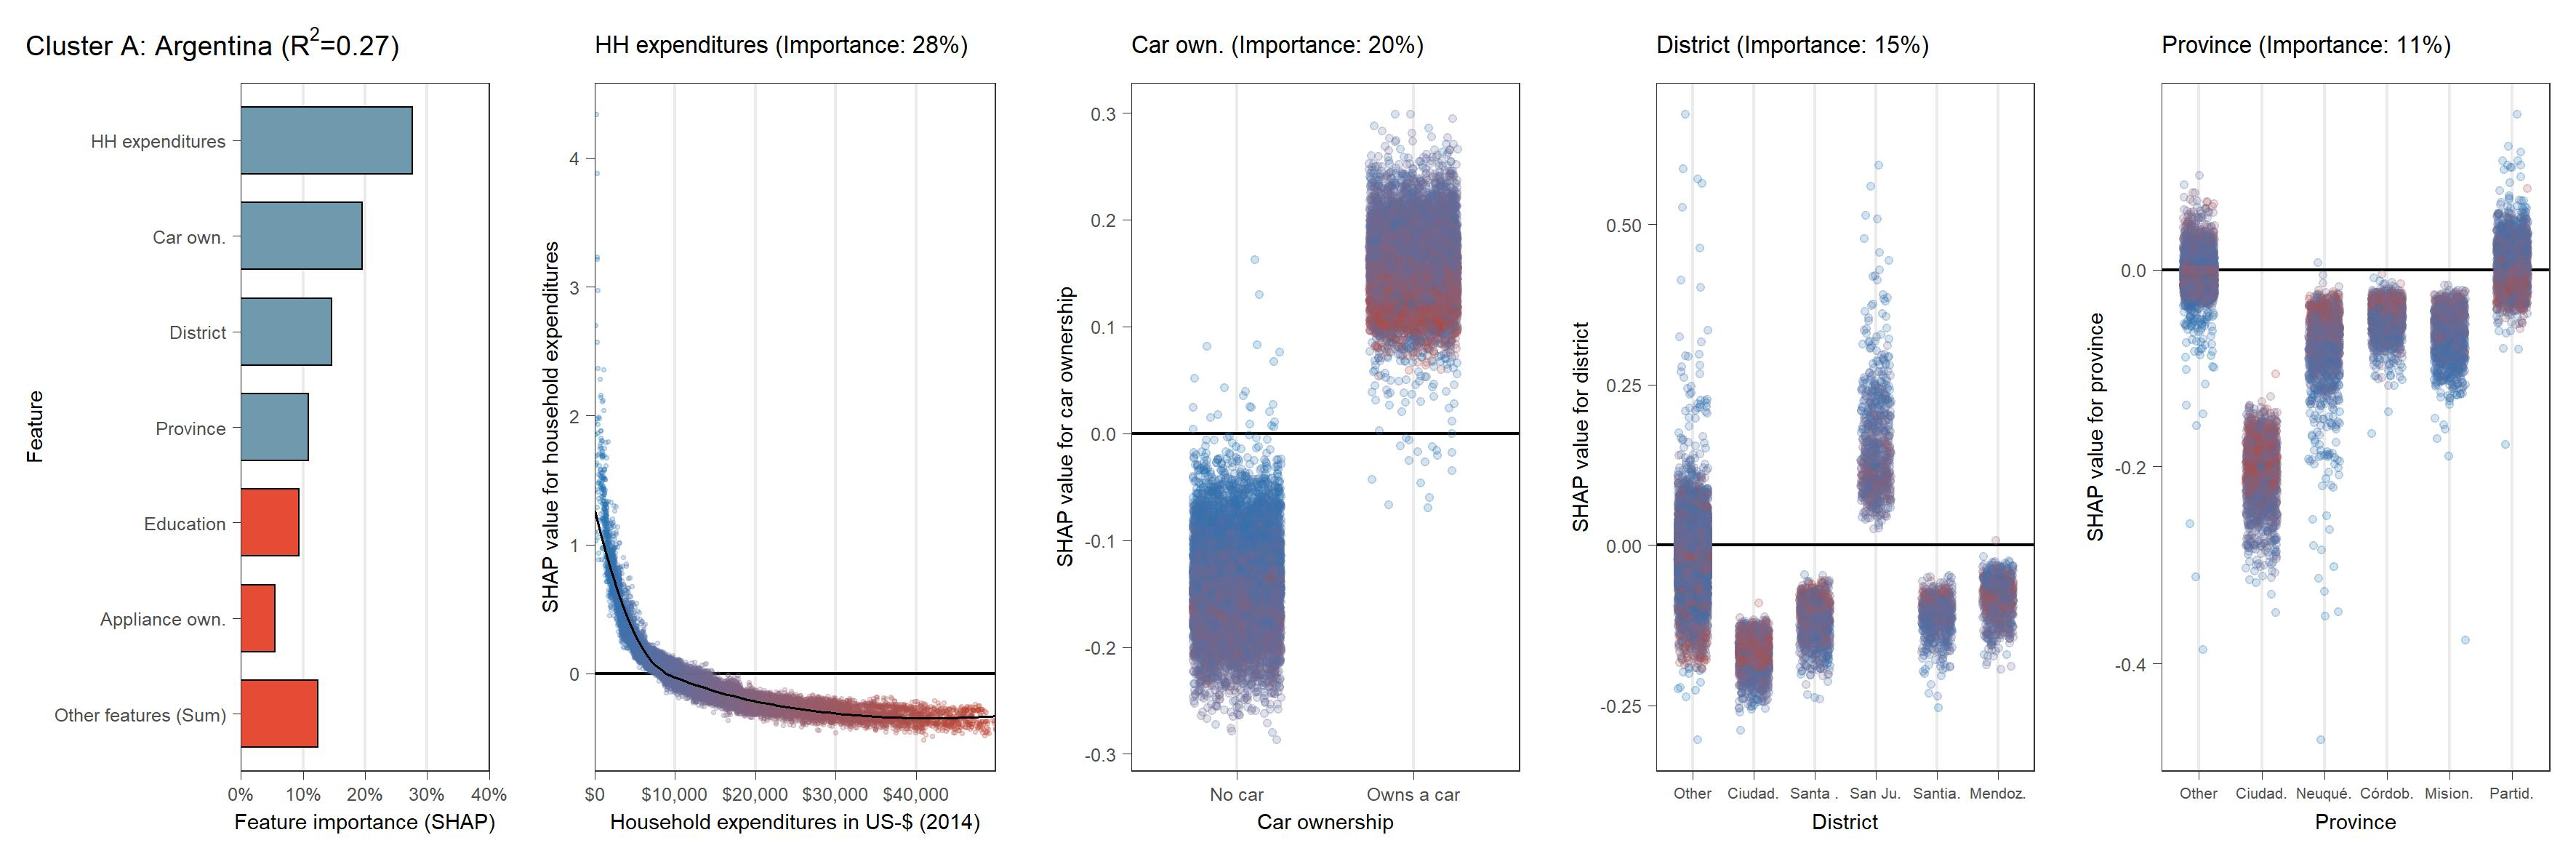
\includegraphics[width=\textwidth]{Figure 5b/Figure_5b_ARG} 
     \end{subfigure}
    \\
    \vspace{0.5cm}
     \begin{subfigure}[b]{\textwidth}
         \centering
         \caption{Partial dependence plot (SHAP) for Australia (cluster A)}
         \label{fig:5b_AUS}
         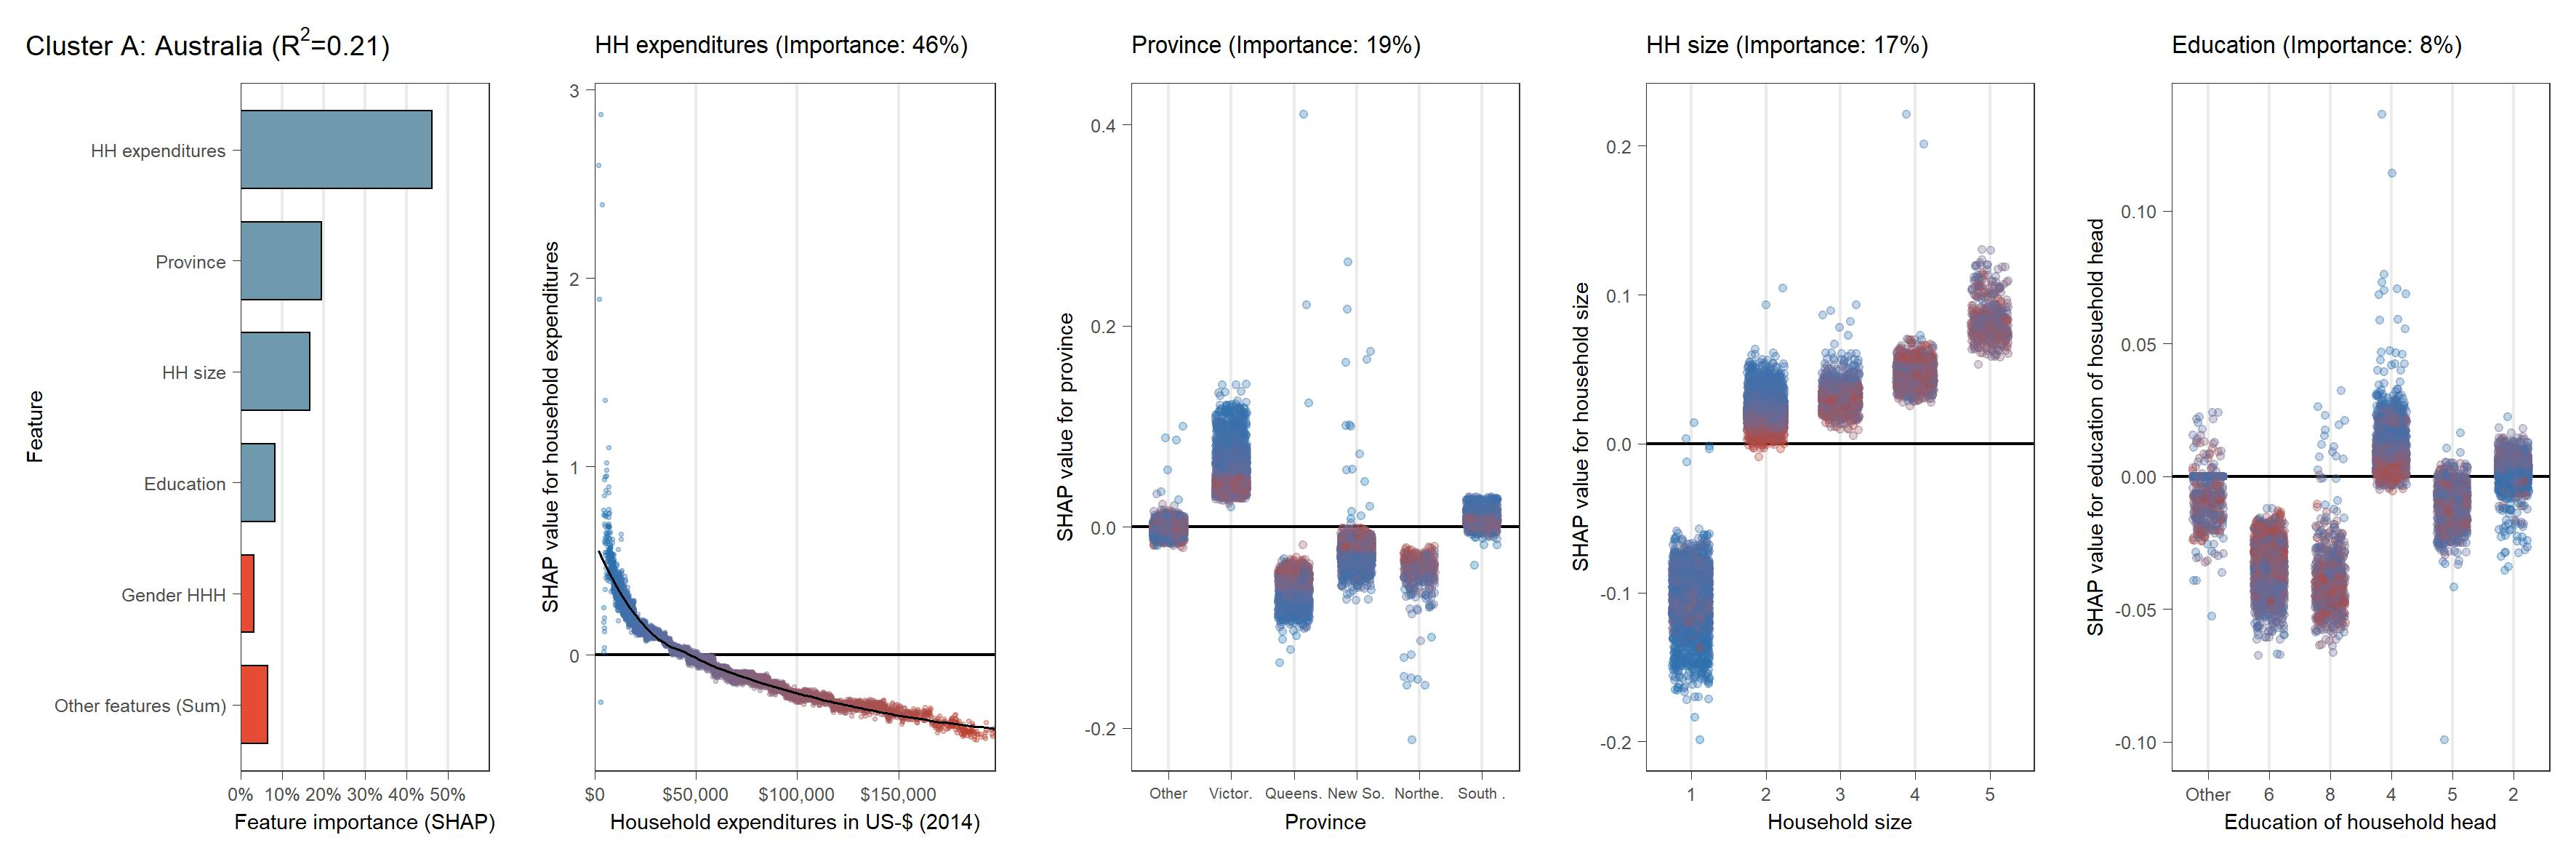
\includegraphics[width=\textwidth]{Figure 5b/Figure_5b_AUS}    \end{subfigure}
    \\
    \vspace{0.5cm}
     \begin{subfigure}[b]{1\textwidth}
     \centering
         \caption{Partial dependence plot (SHAP) for Austria (cluster A)}
         \label{fig:5b_AUT}
         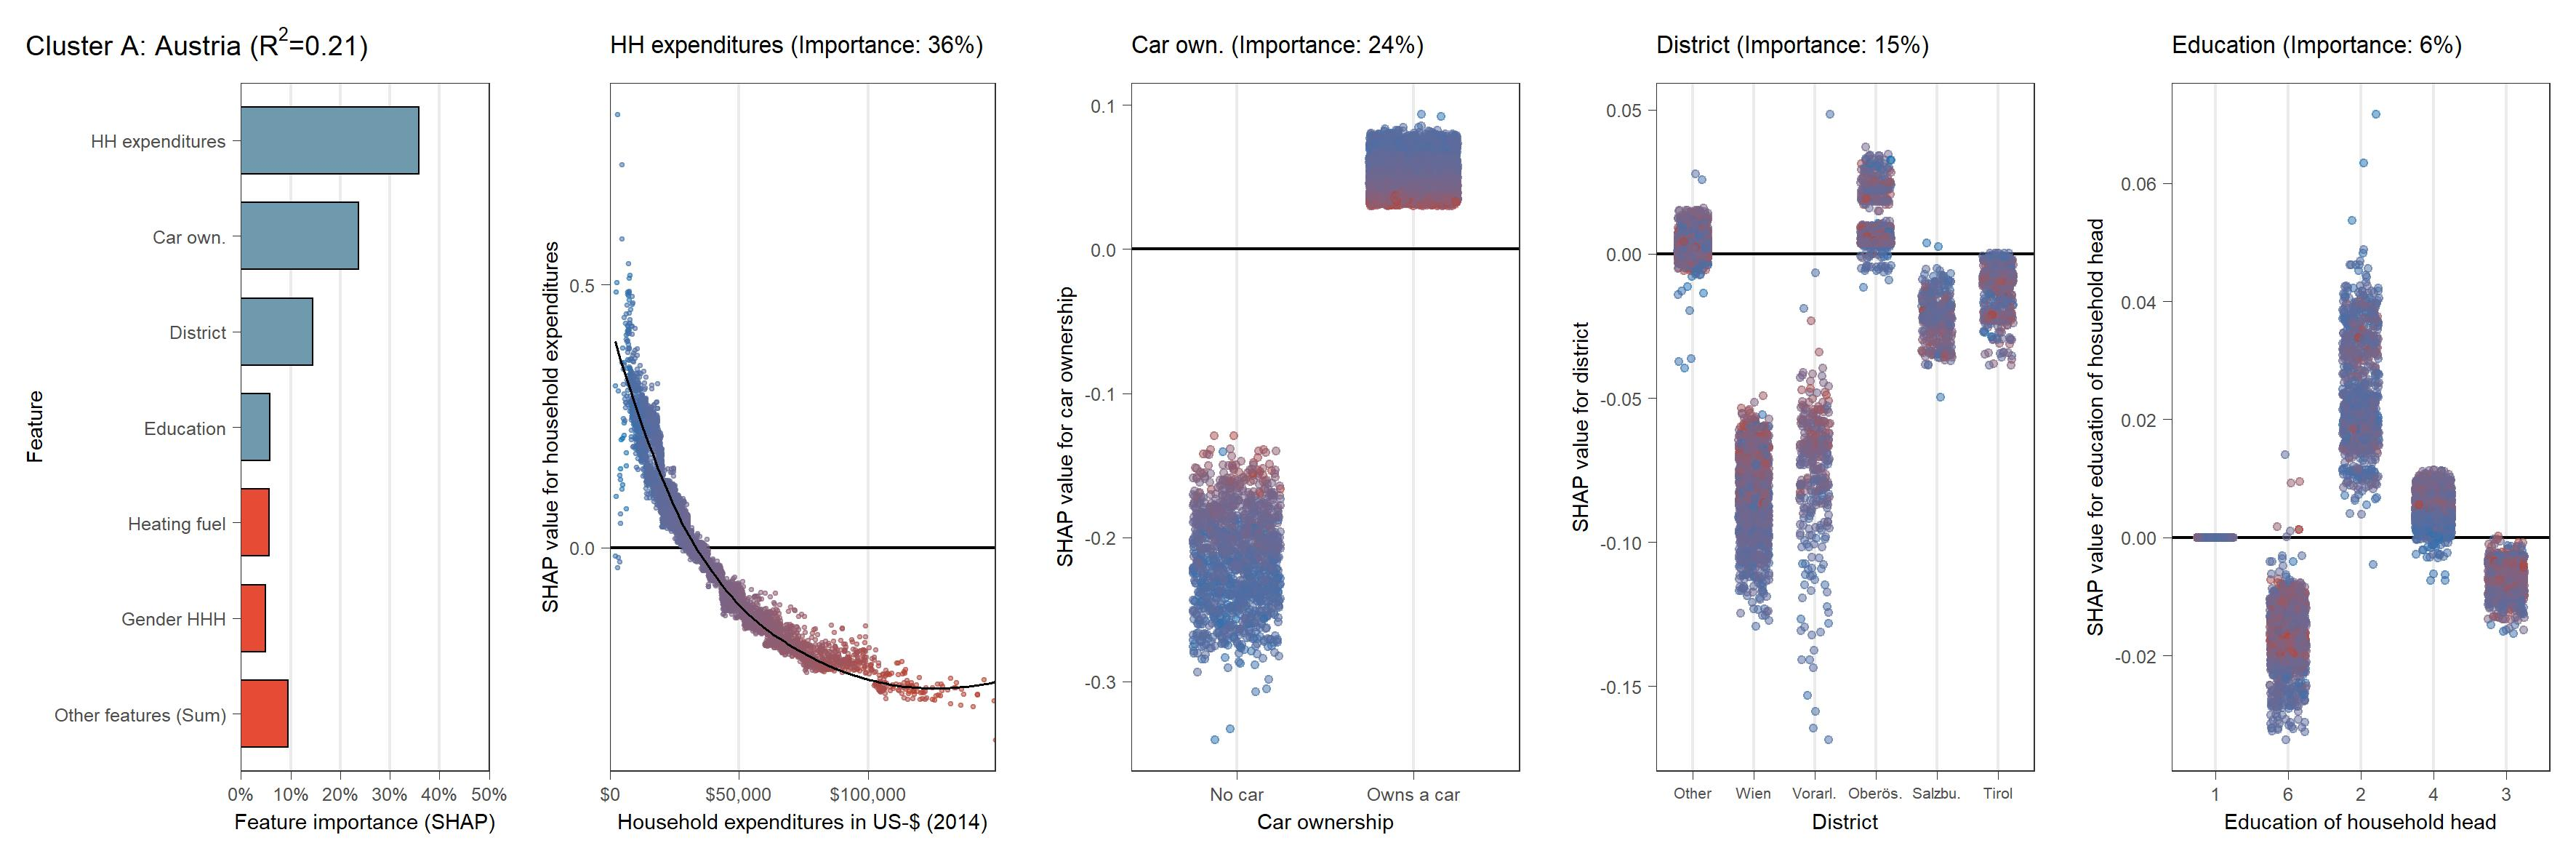
\includegraphics[width=\textwidth]{Figure 5b/Figure_5b_AUT} 
         \end{subfigure}
     \\
     \vspace{0.5cm}
        \begin{subcaption2}
     This figure shows SHAP-values for predicting carbon intensity over feature values for 88 countries in alphabetical order for six country-clusters. The bar chart displays normalized average absolute SHAP-values for all features. Features with less than 3\% of normalized SHAP-values are subsumed as "Other features (Sum)". Panels show SHAP-values over total household expenditures for all countries and for the three most important features in each country besides total household expenditures. Colors represent household expenditures with blue (red) colors indicating lower (higher) household expenditures.
     \end{subcaption2}
     \end{figure}
     
\begin{figure}[ht!]\ContinuedFloat
    \centering
   \begin{subfigure}[b]{\textwidth}
   \centering
         \caption{Partial dependence plot (SHAP) for Belgium (cluster A)}
         \label{fig:5b_BEL}
         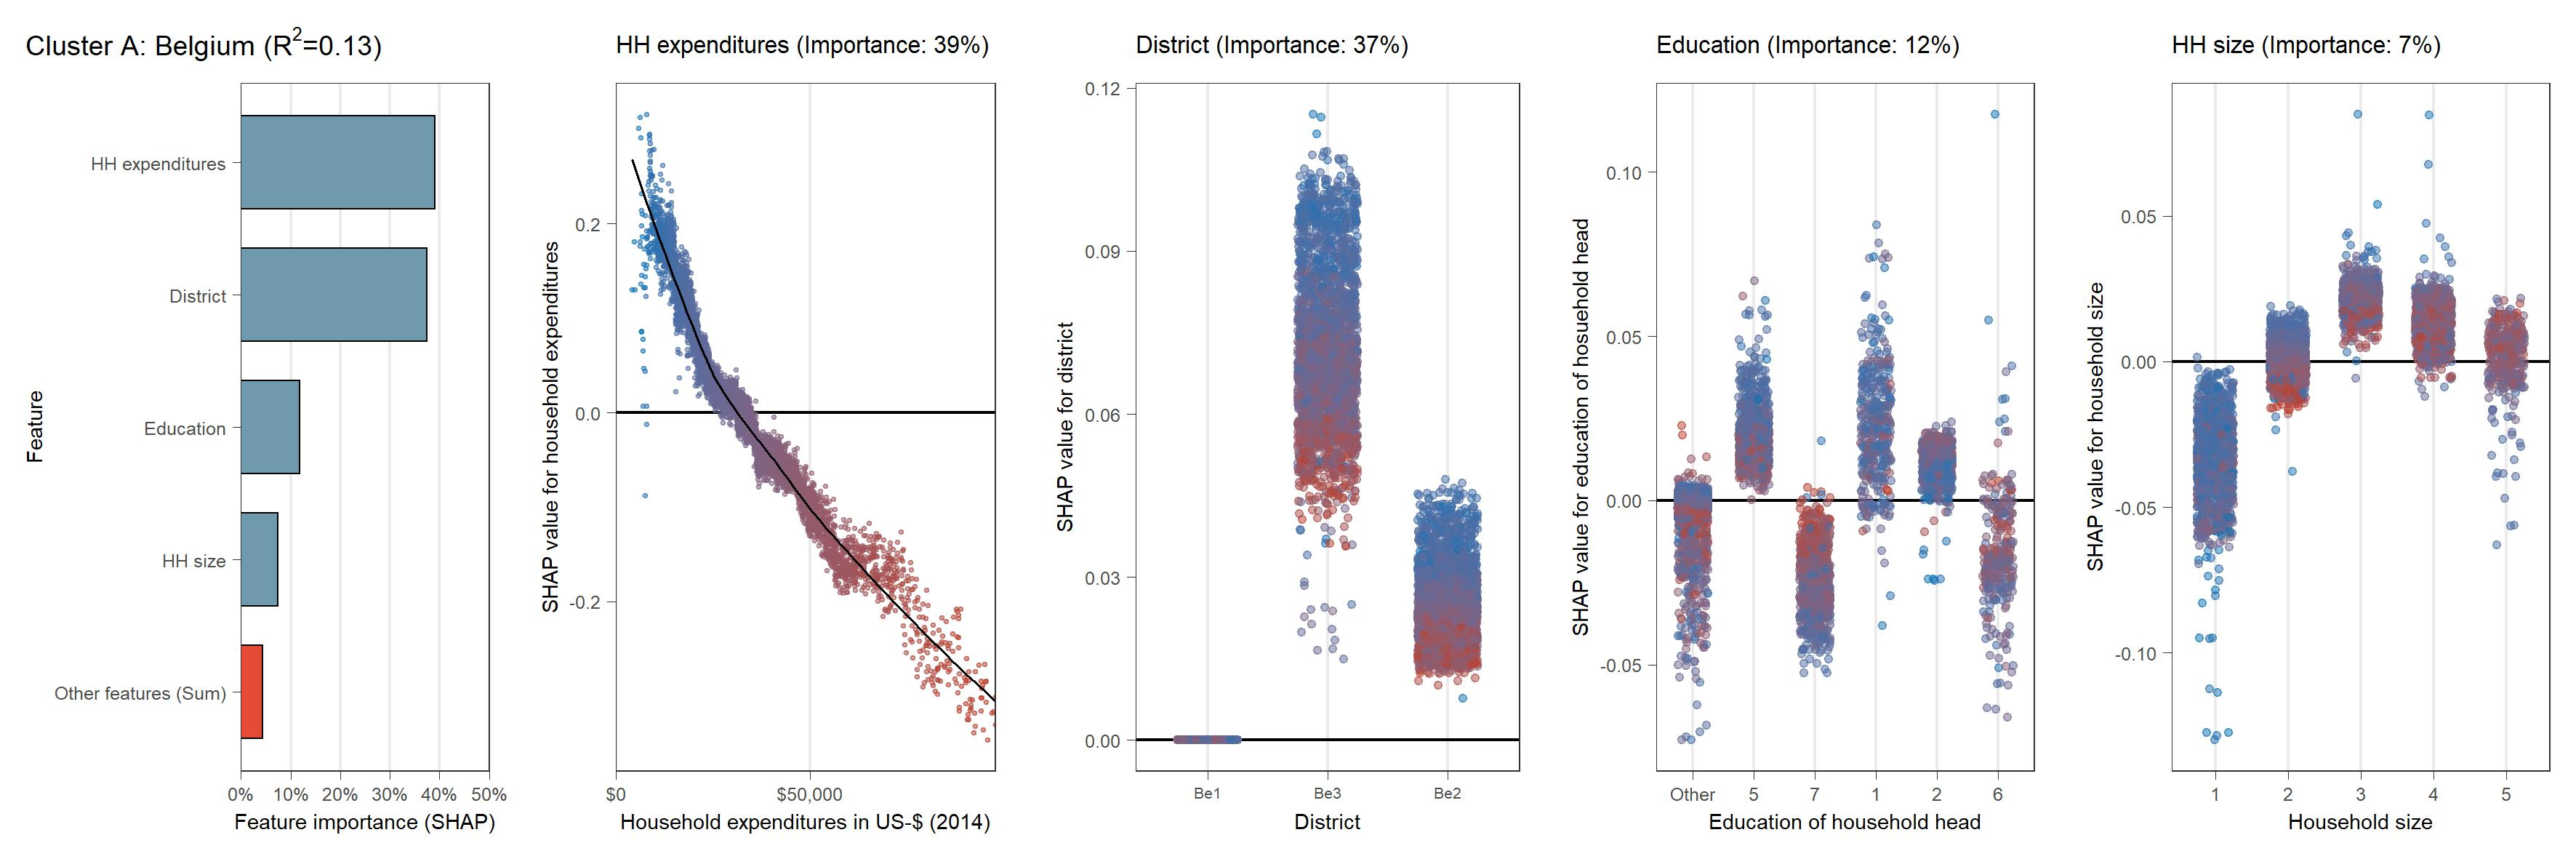
\includegraphics[width=\textwidth]{Figure 5b/Figure_5b_BEL}
         \end{subfigure}
    \\
    \vspace{0.5cm}
   \begin{subfigure}[b]{\textwidth}
   \centering
         \caption{Partial dependence plot (SHAP) for Bangladesh (cluster A)}
         \label{fig:5b_BGD}
         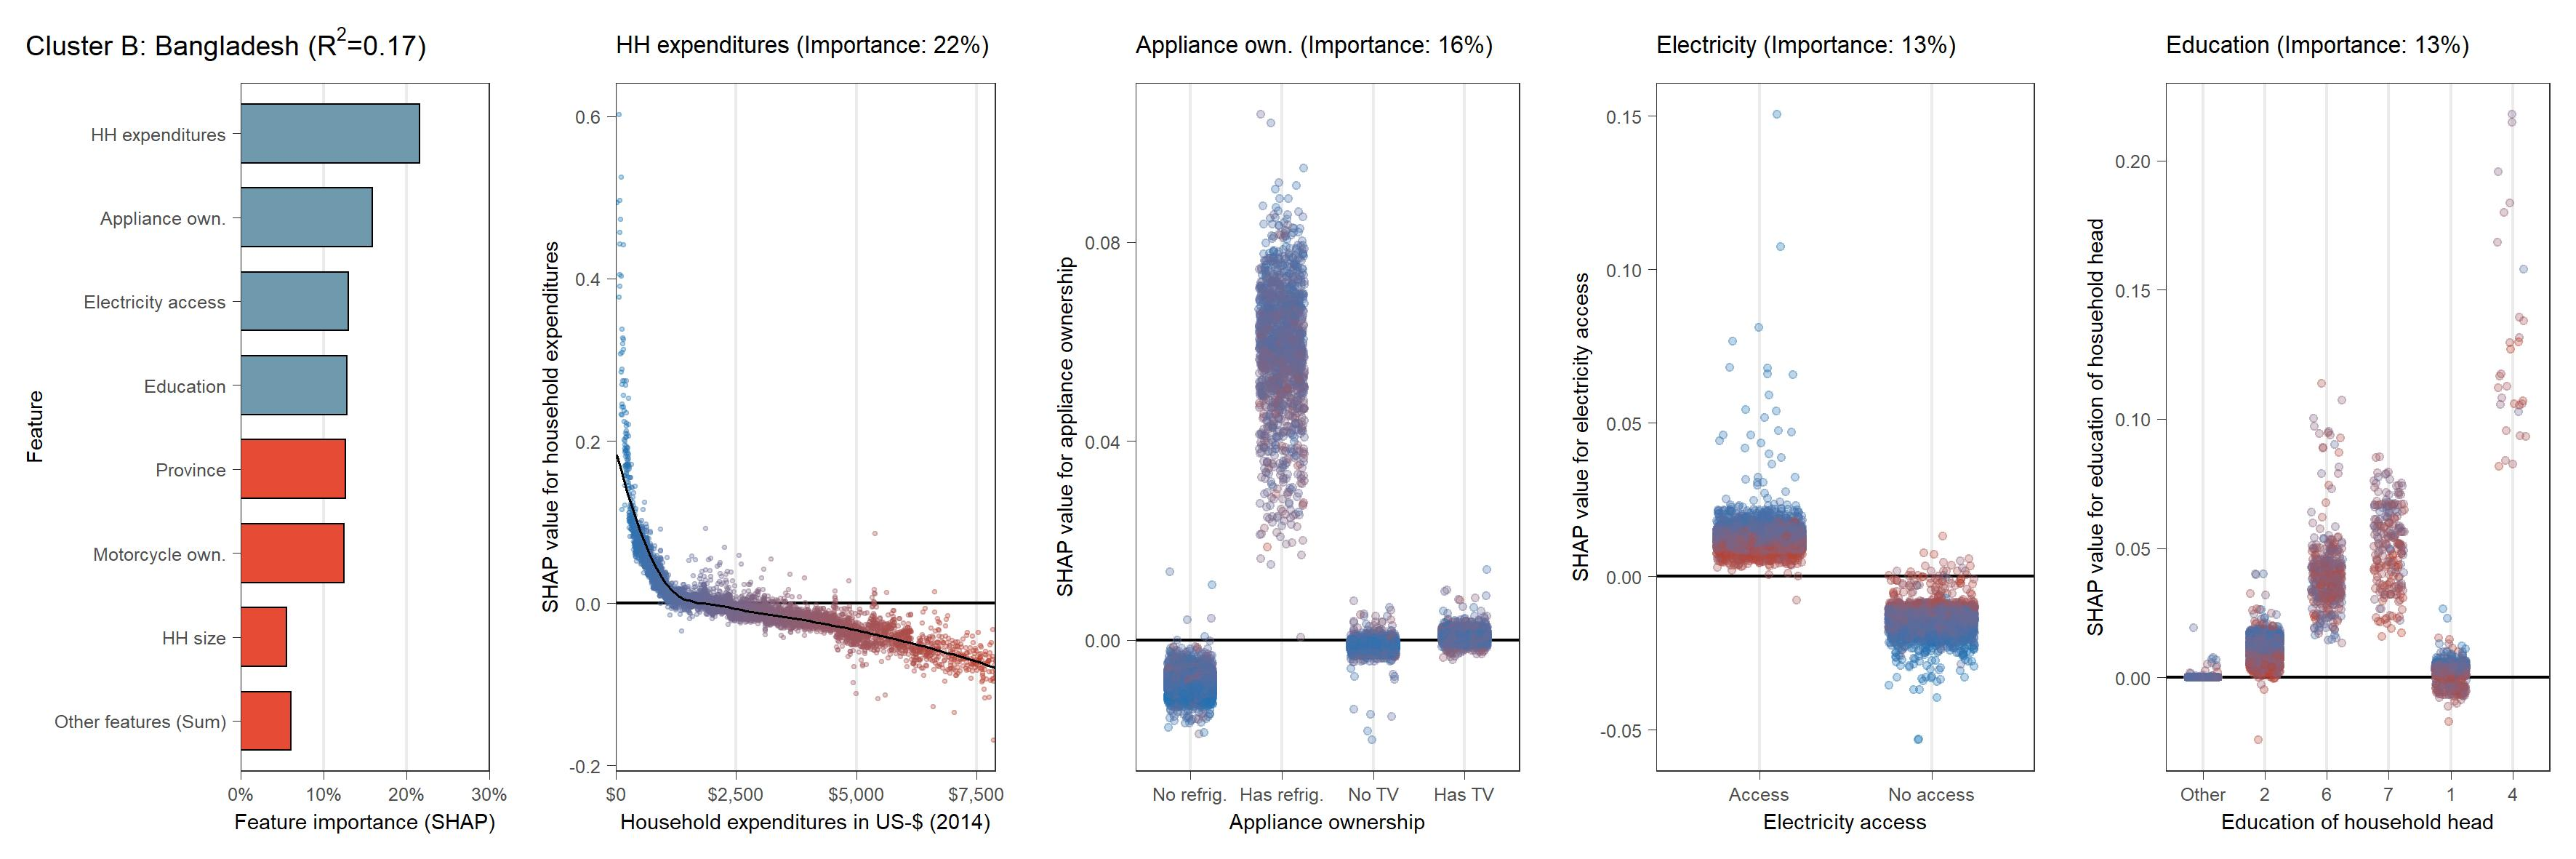
\includegraphics[width=\textwidth]{Figure 5b/Figure_5b_BGD} 
         \end{subfigure}
    \\
    \vspace{0.5cm}
   \begin{subfigure}[b]{\textwidth}
         \centering
         \caption{Partial dependence plot (SHAP) for Bulgaria (cluster A)}
         \label{fig:5b_BGR}
         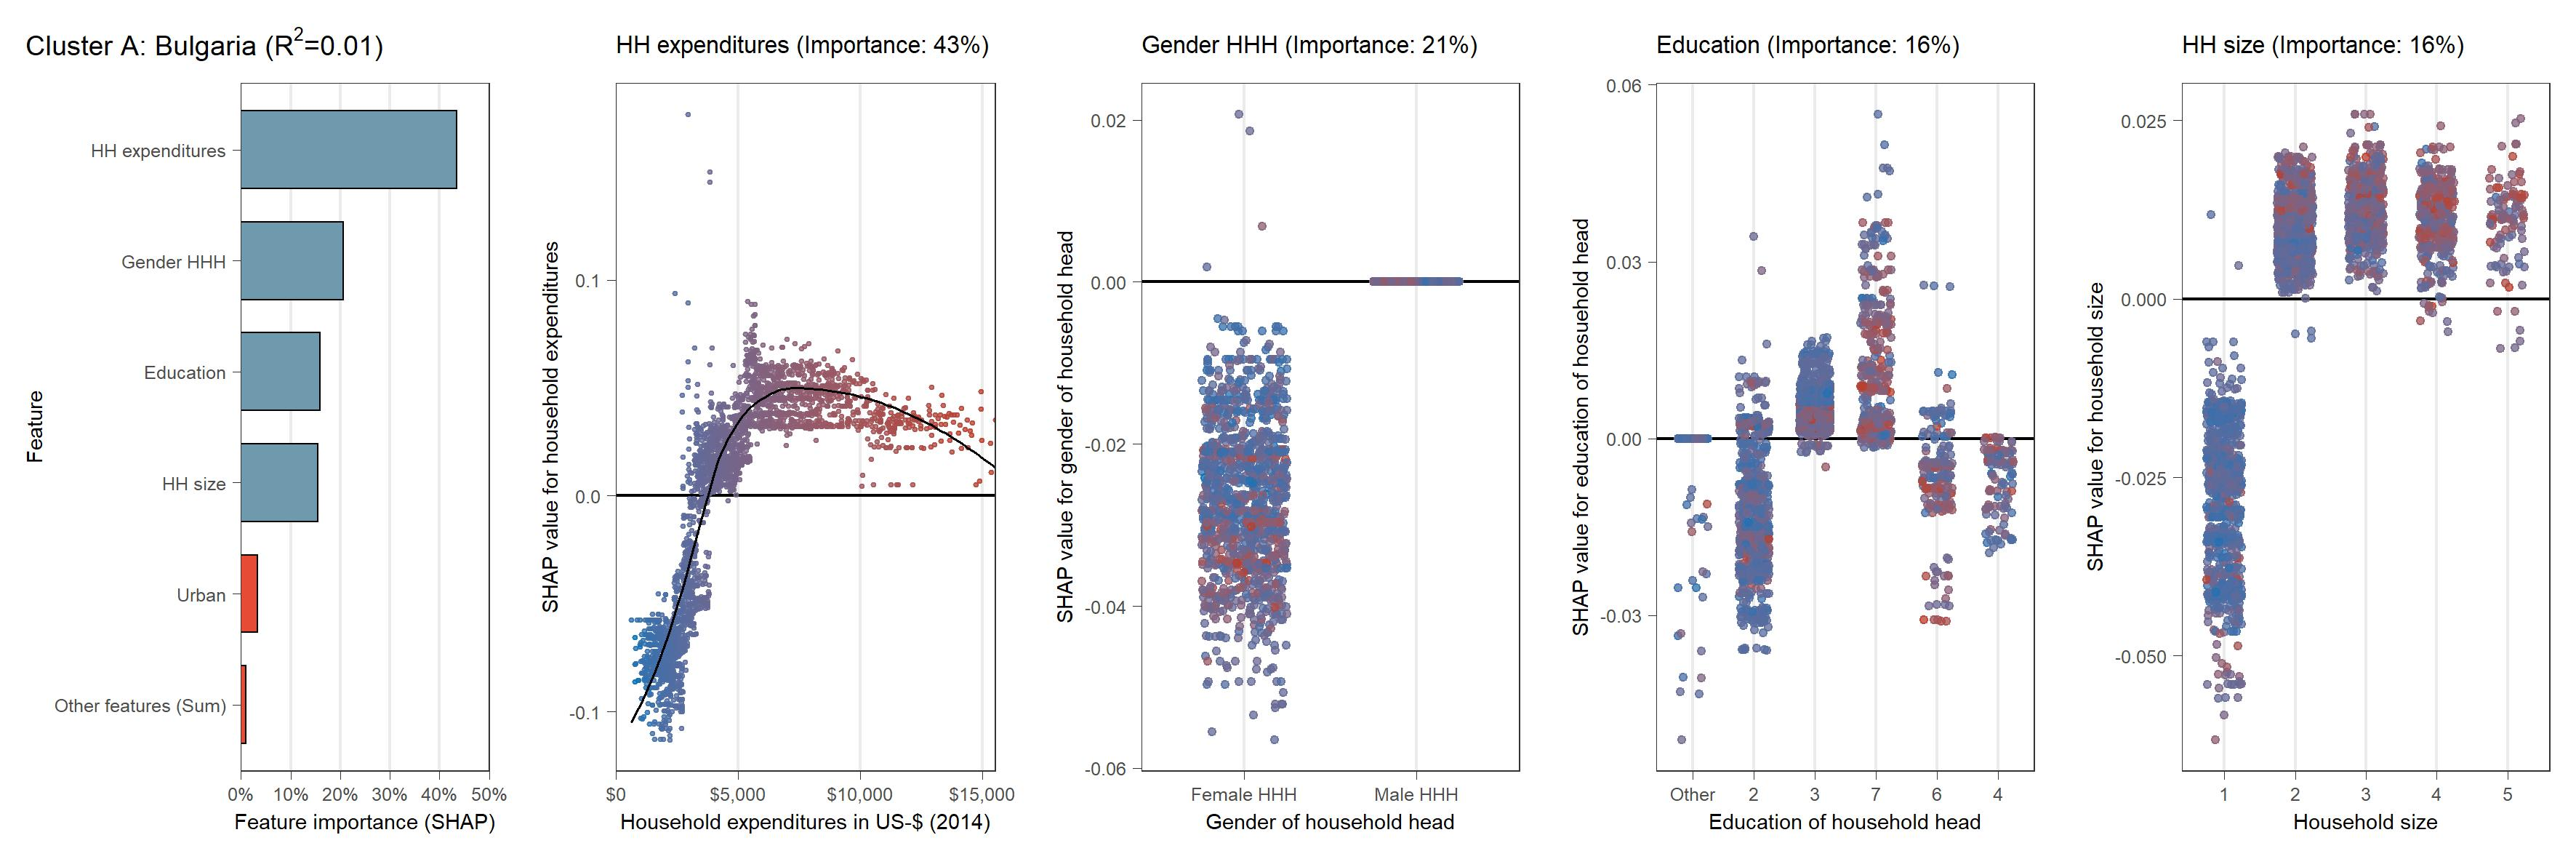
\includegraphics[width=\textwidth]{Figure 5b/Figure_5b_BGR}     \end{subfigure}
    \\
    \vspace{0.5cm}
    \begin{subcaption2}
     This figure shows SHAP-values for predicting carbon intensity over feature values for 88 countries in alphabetical order for six country-clusters. The bar chart displays normalized average absolute SHAP-values for all features. Features with less than 3\% of normalized SHAP-values are subsumed as "Other features (Sum)". Panels show SHAP-values over total household expenditures for all countries and for the three most important features in each country besides total household expenditures. Colors represent household expenditures with blue (red) colors indicating lower (higher) household expenditures.
     \end{subcaption2}
\end{figure}

\begin{figure}[ht!]\ContinuedFloat
    \centering
   \begin{subfigure}[b]{\textwidth}
         \centering
         \caption{Partial dependence plot (SHAP) for Brazil (cluster A)}
         \label{fig:5b_BRA}
         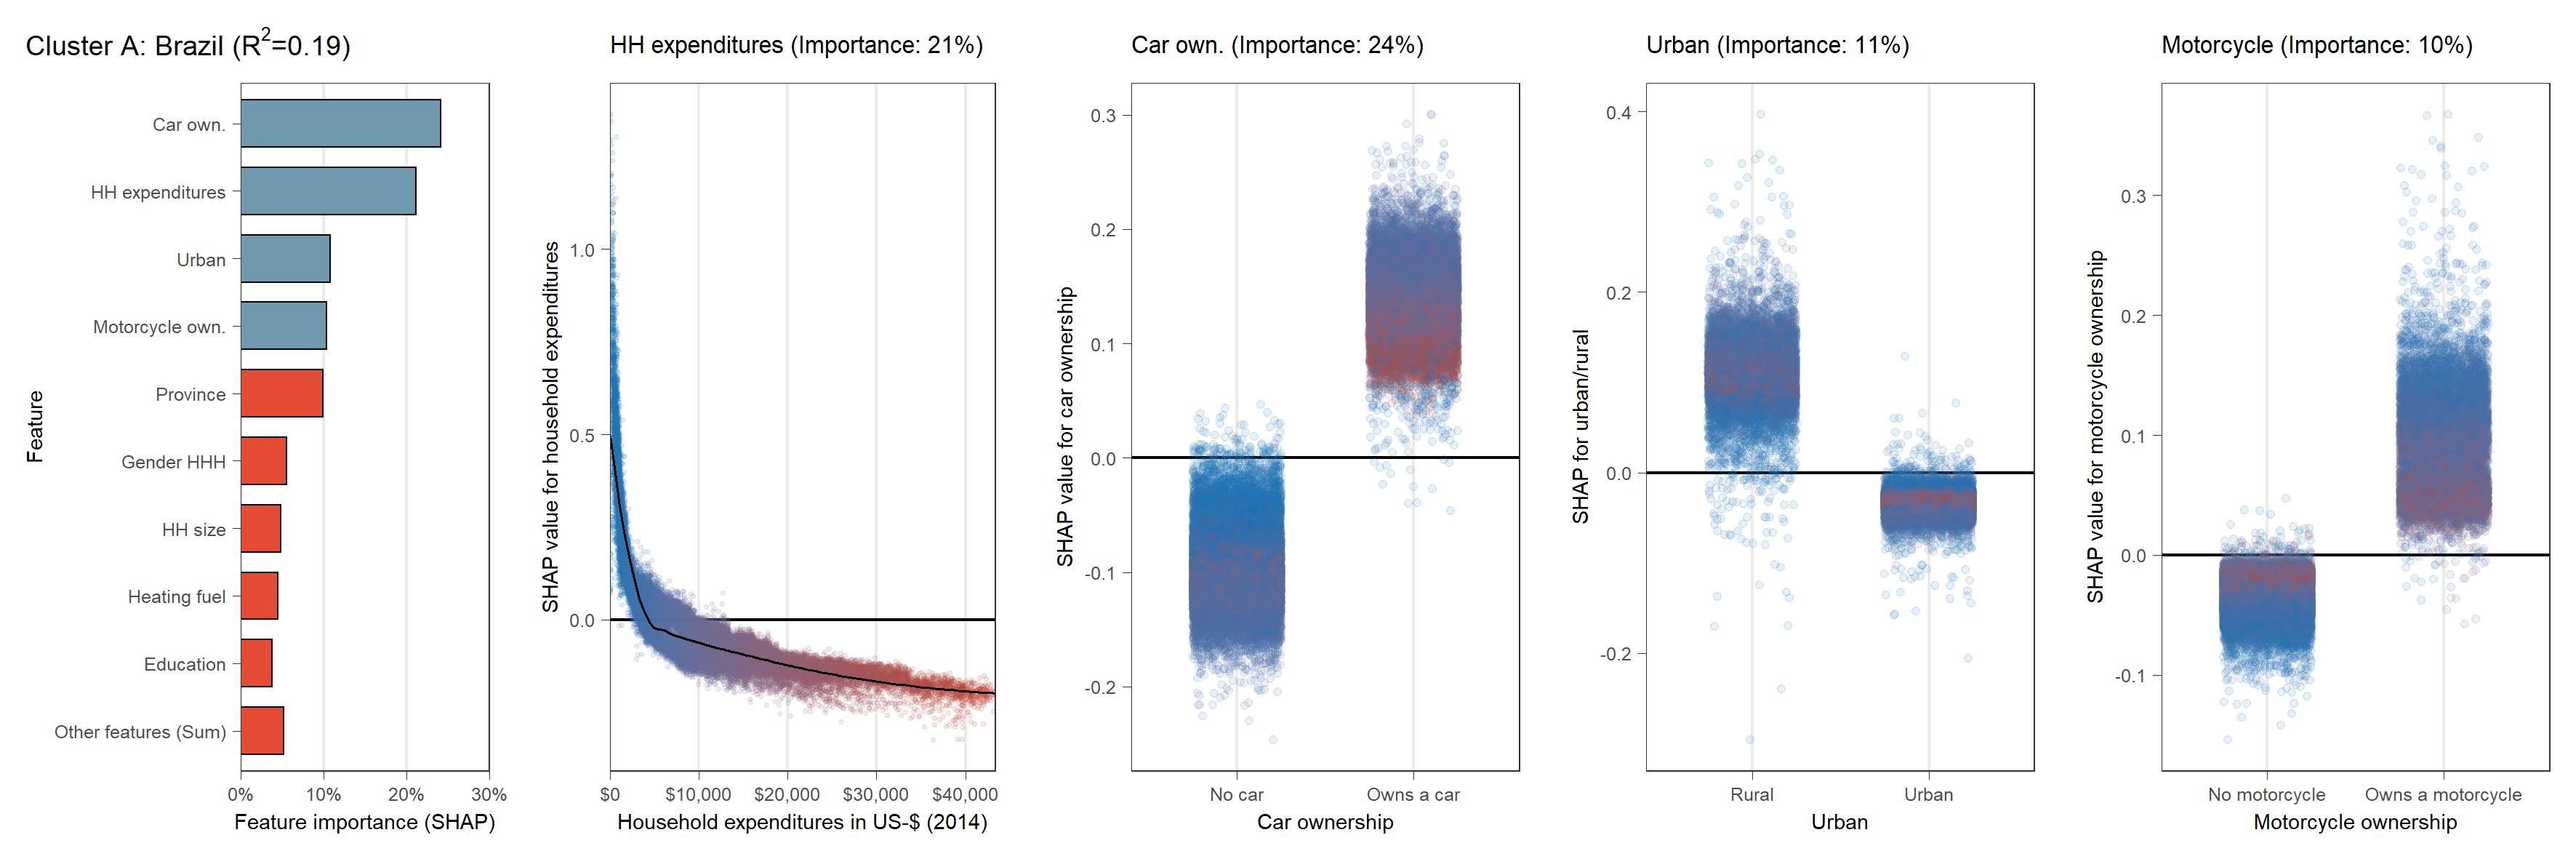
\includegraphics[width=\textwidth]{Figure 5b/Figure_5b_BRA}
         \end{subfigure}
    \\
    \vspace{0.5cm}
   \begin{subfigure}[b]{\textwidth}
         \centering
         \caption{Partial dependence plot (SHAP) for Canada (cluster A)}
         \label{fig:5b_CAN}
         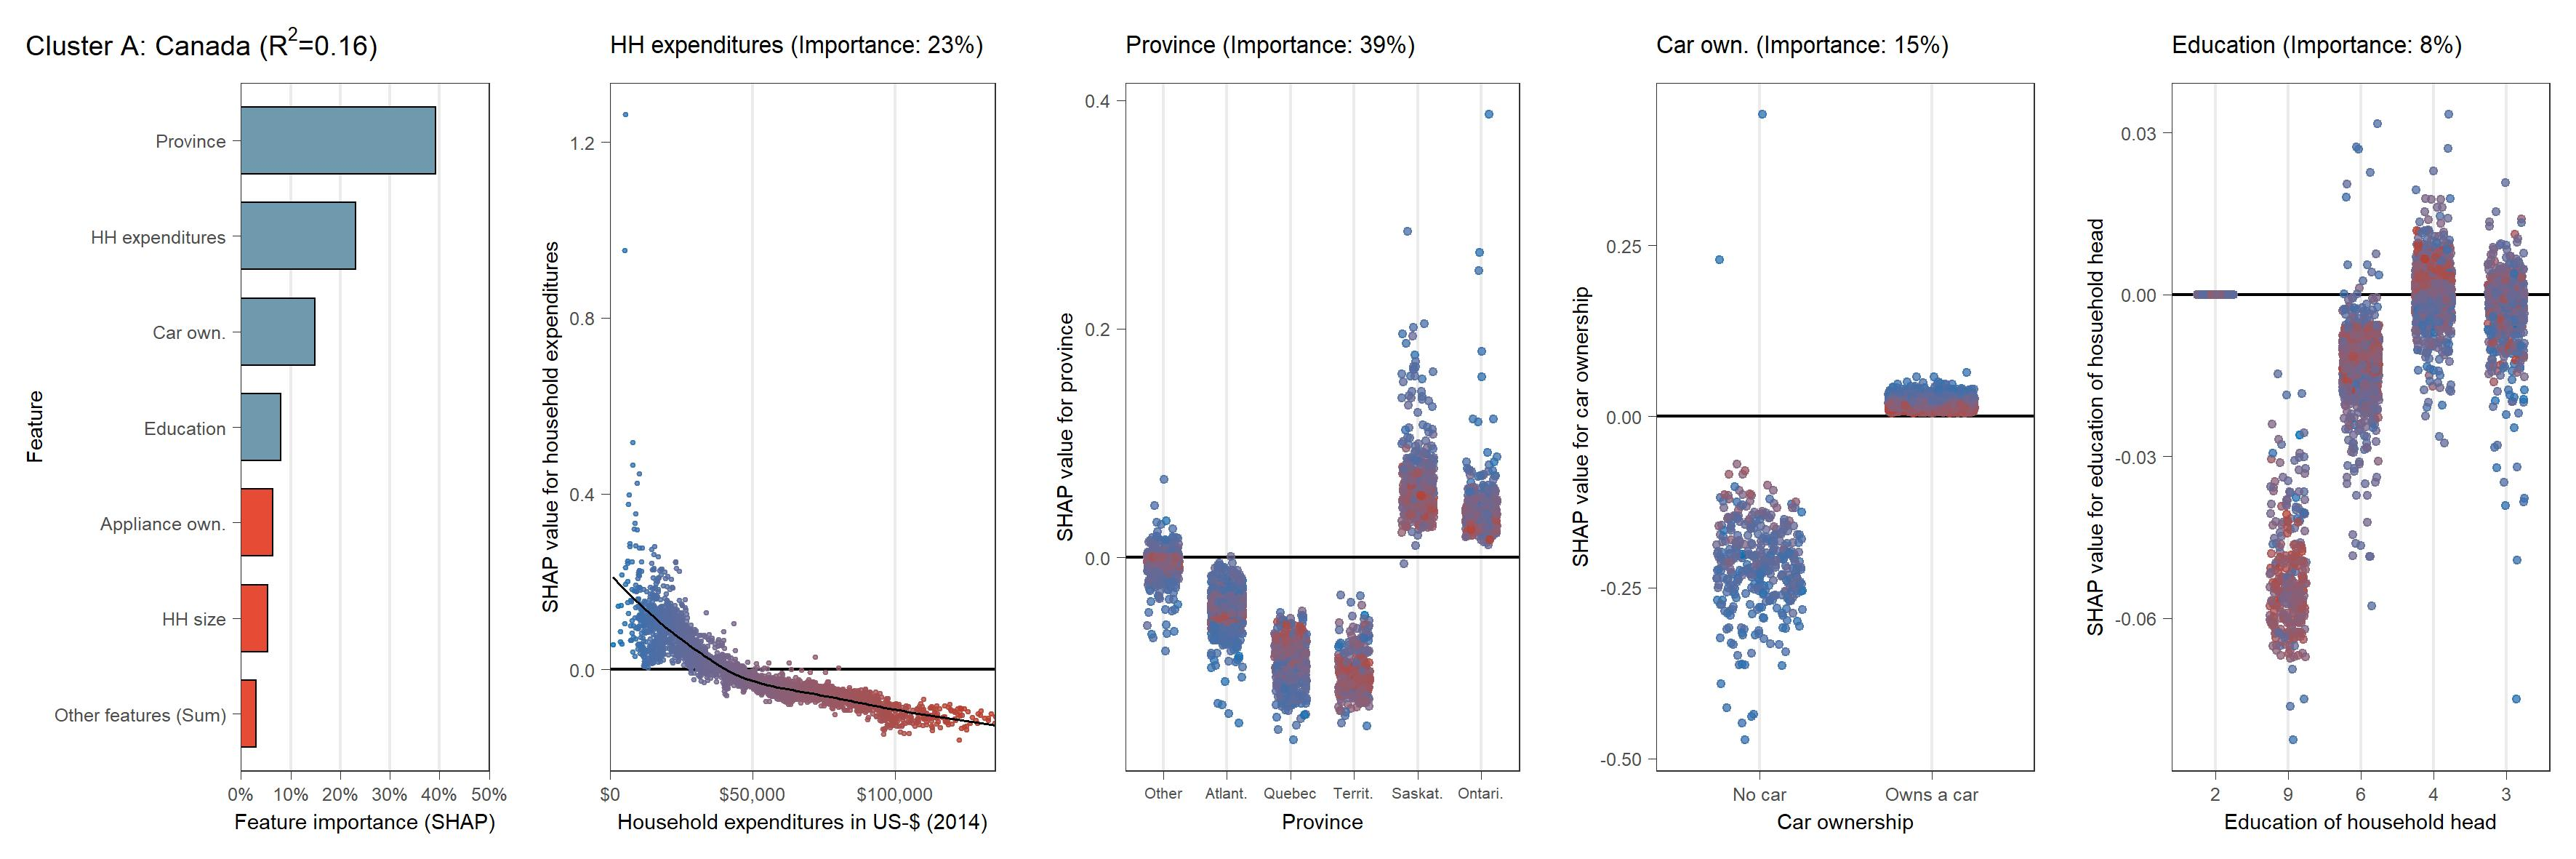
\includegraphics[width=\textwidth]{Figure 5b/Figure_5b_CAN}
         \end{subfigure}
    \\
    \vspace{0.5cm}
   \begin{subfigure}[b]{\textwidth}
         \centering
         \caption{Partial dependence plot (SHAP) for Switzerland (cluster A)}
         \label{fig:5b_CHE}
         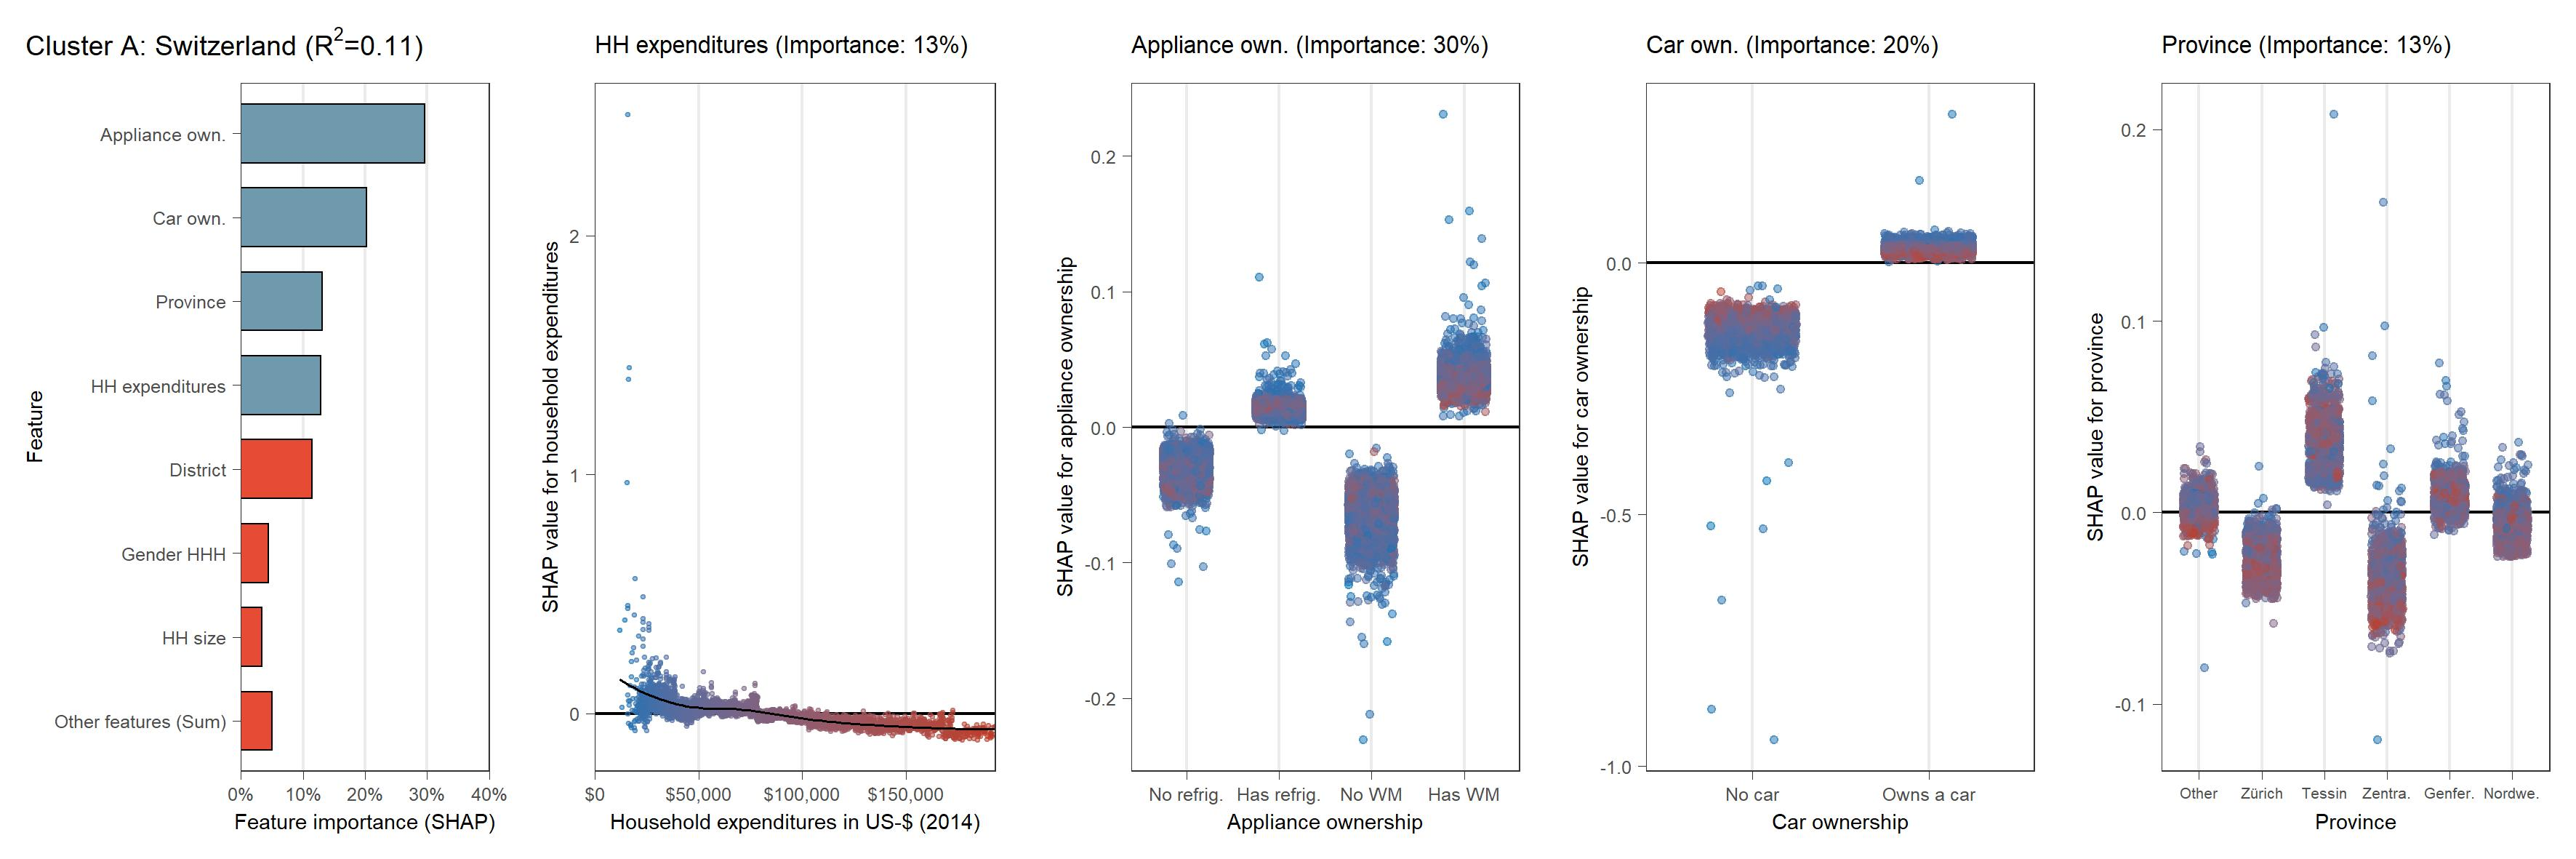
\includegraphics[width=\textwidth]{Figure 5b/Figure_5b_CHE}
    \end{subfigure}
    \\
    \vspace{0.5cm}
    \begin{subcaption2}
     This figure shows SHAP-values for predicting carbon intensity over feature values for 88 countries in alphabetical order for six country-clusters. The bar chart displays normalized average absolute SHAP-values for all features. Features with less than 3\% of normalized SHAP-values are subsumed as "Other features (Sum)". Panels show SHAP-values over total household expenditures for all countries and for the three most important features in each country besides total household expenditures. Colors represent household expenditures with blue (red) colors indicating lower (higher) household expenditures.
     \end{subcaption2}
\end{figure}

\begin{figure}[ht!]\ContinuedFloat
    \centering
   \begin{subfigure}[b]{\textwidth}
         \centering
         \caption{Partial dependence plot (SHAP) for Chile (cluster A)}
         \label{fig:5b_CHL}
         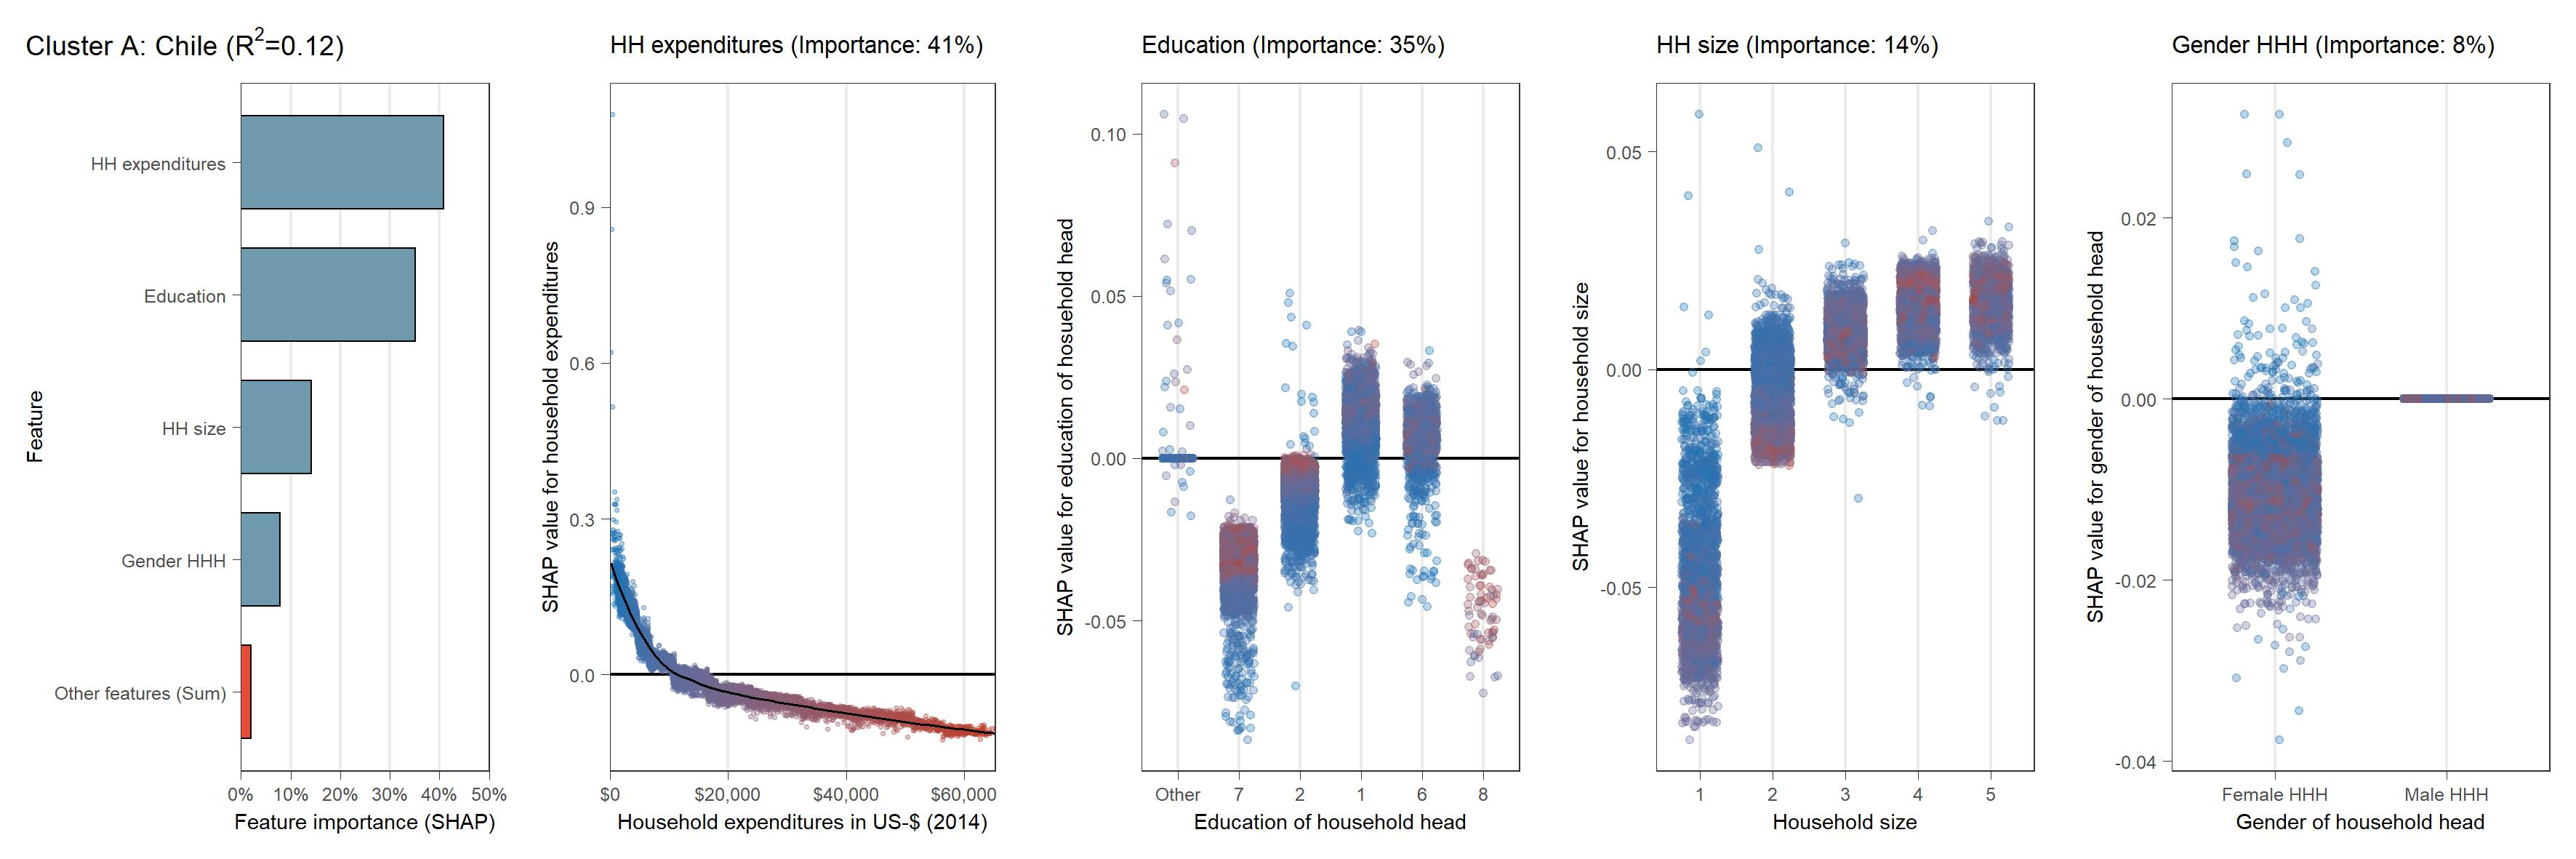
\includegraphics[width=\textwidth]{Figure 5b/Figure_5b_CHL}
         \end{subfigure}
    \\
    \vspace{0.5cm}
   \begin{subfigure}[b]{\textwidth}
      \centering
      \caption{Partial dependence plot (SHAP) for Colombia (cluster A)}
      \label{fig:5b_COL}
      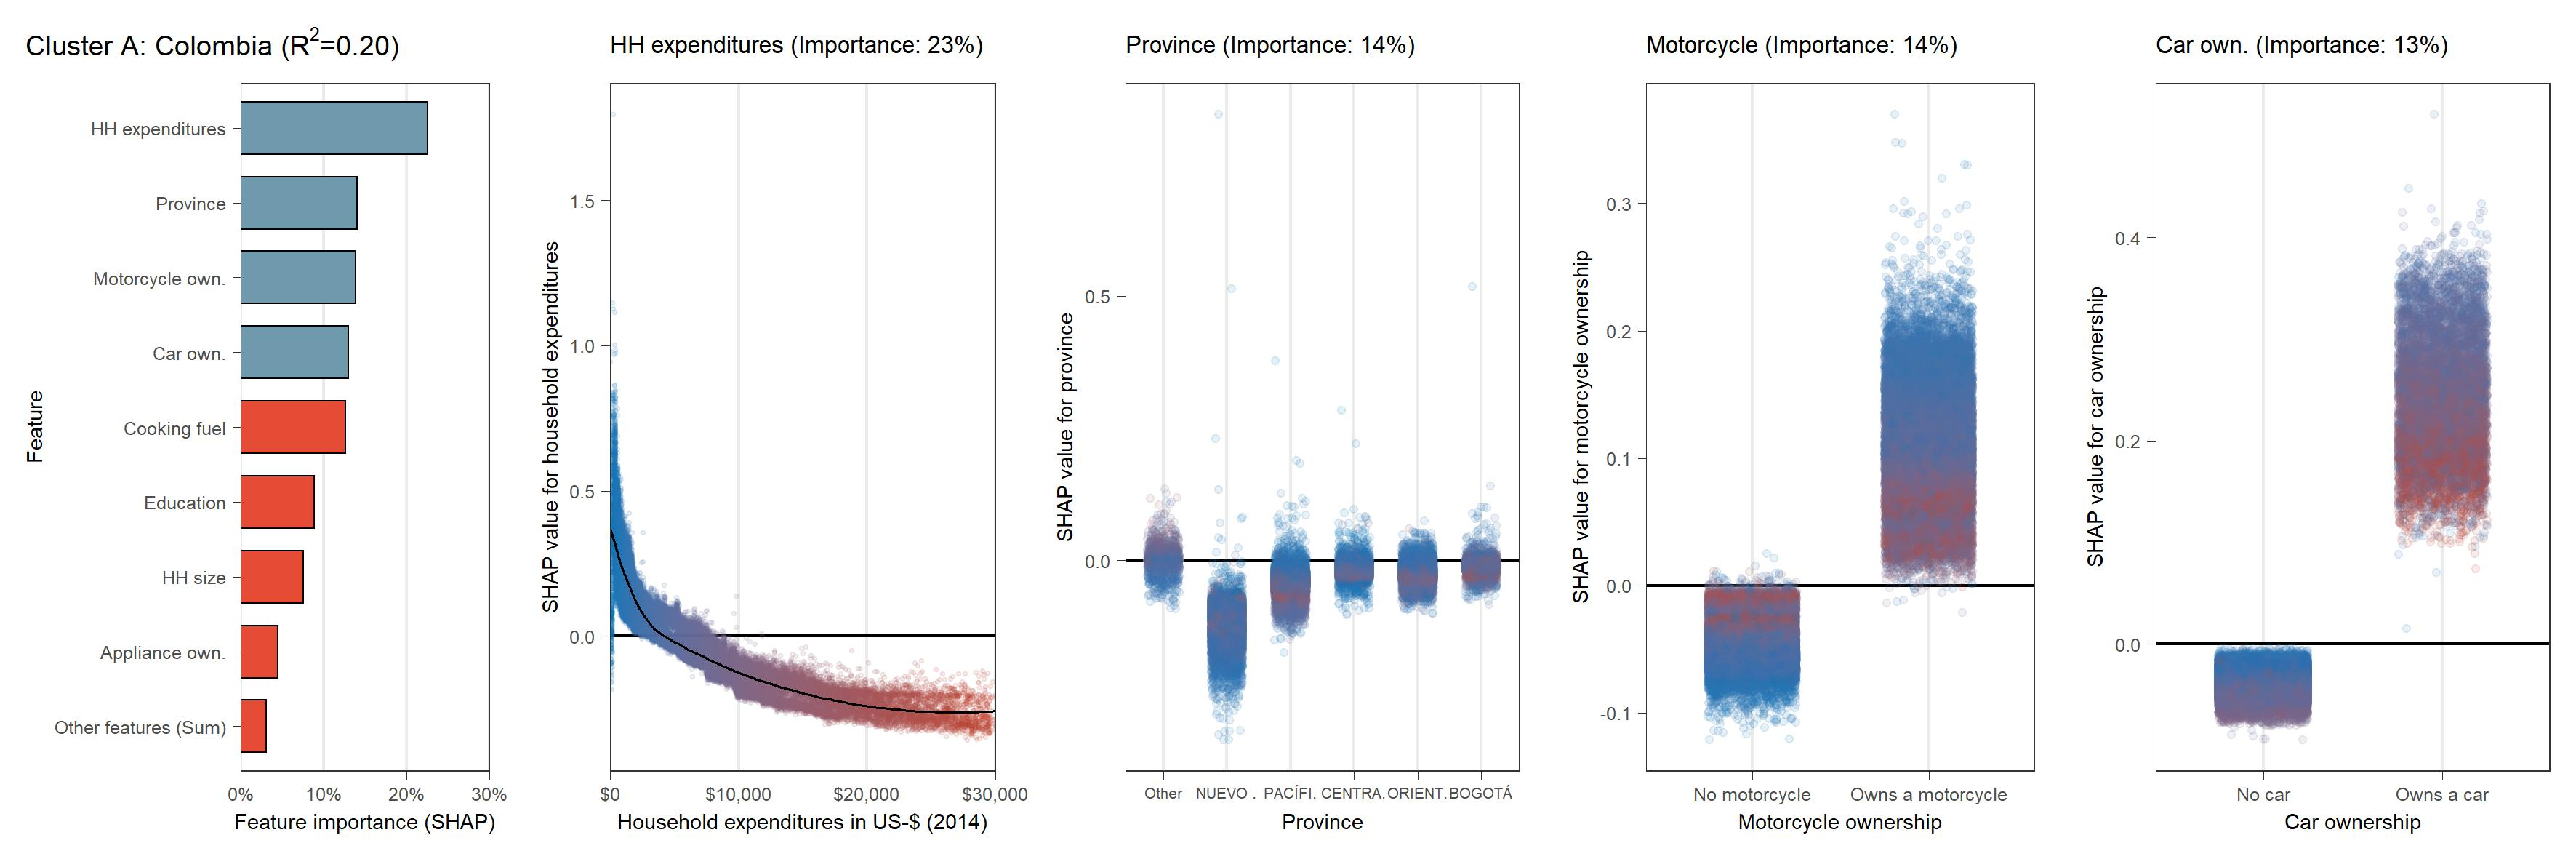
\includegraphics[width=\textwidth]{Figure 5b/Figure_5b_COL}       
     \end{subfigure}
    \\
    \vspace{0.5cm}
   \begin{subfigure}[b]{\textwidth}
         \centering
         \caption{Partial dependence plot (SHAP) for Cyprus (cluster A)}
         \label{fig:5b_CYP}
         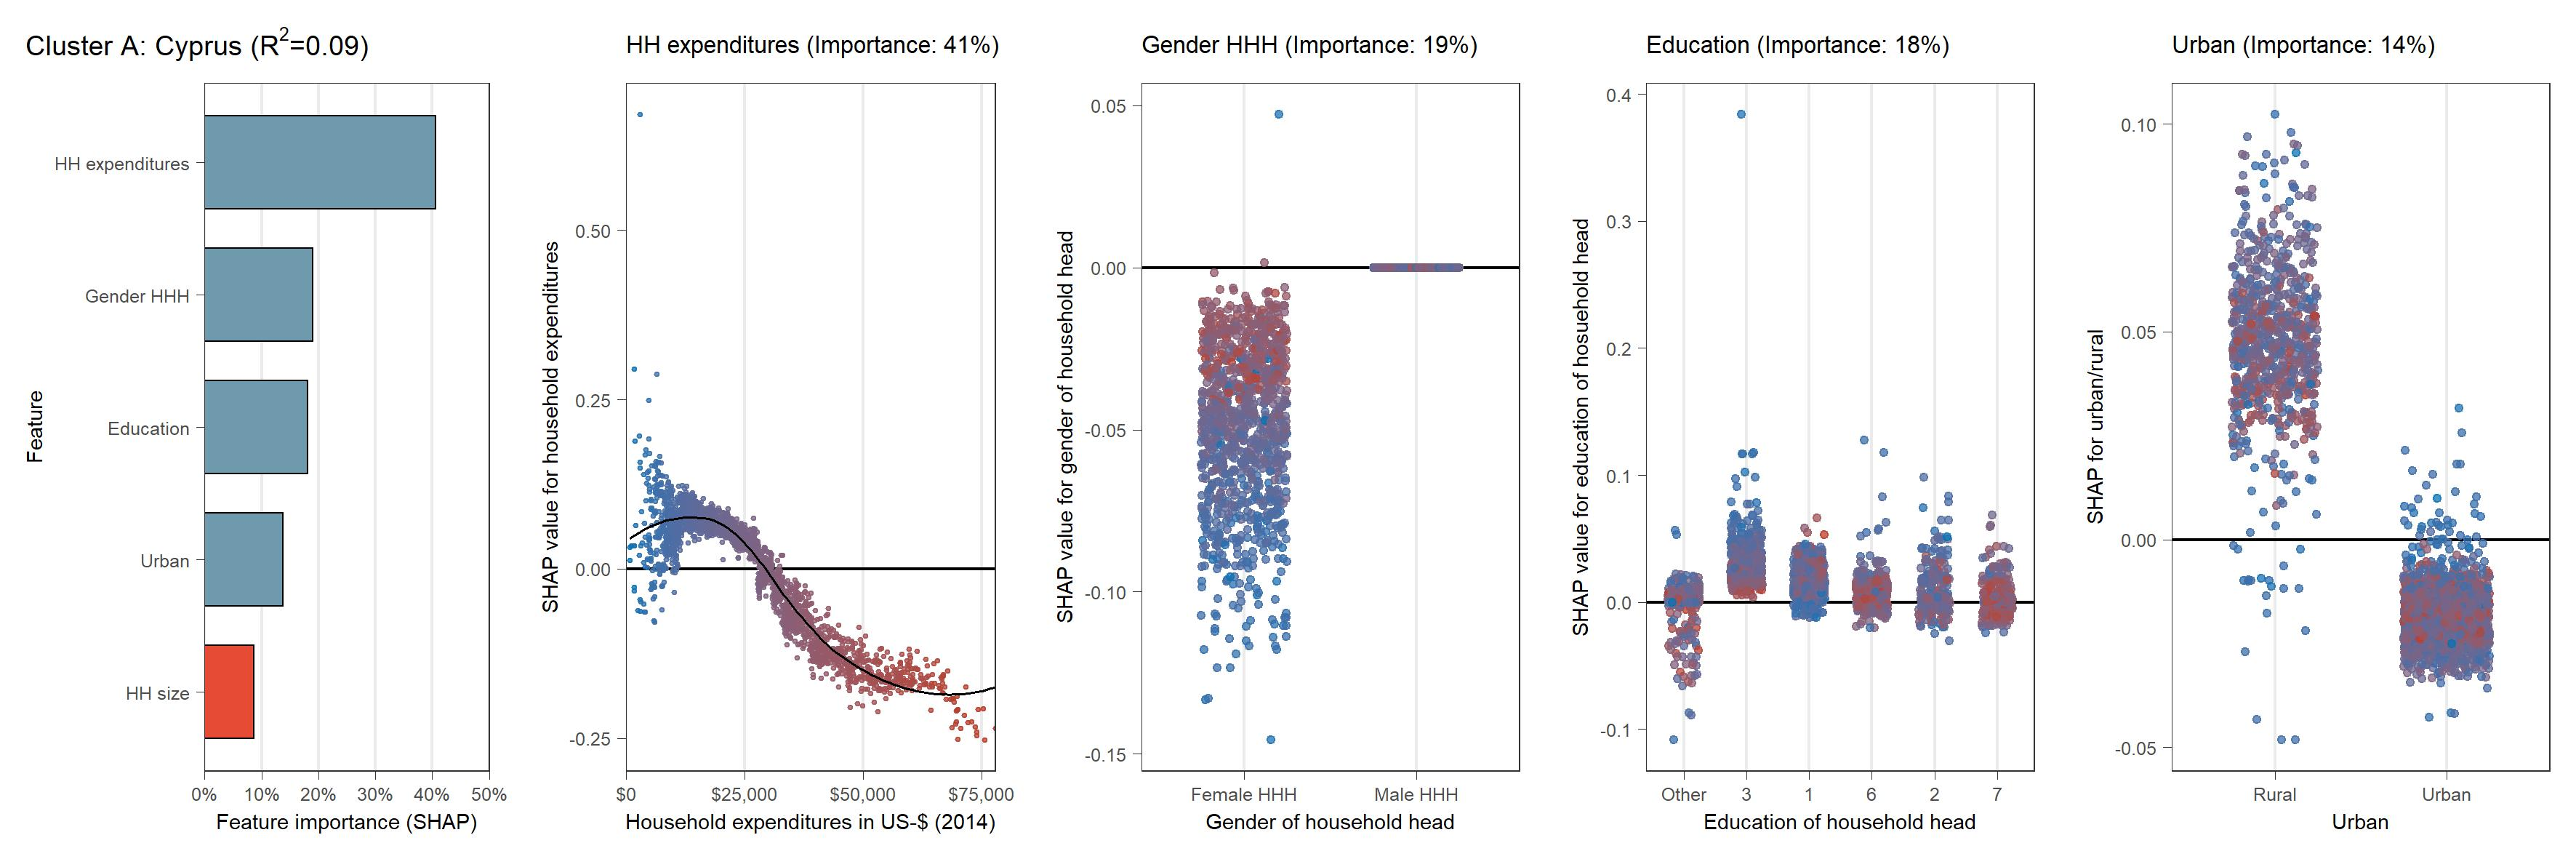
\includegraphics[width=\textwidth]{Figure 5b/Figure_5b_CYP}
         \end{subfigure}
    \\
    \vspace{0.5cm}
    \begin{subcaption2}
     This figure shows SHAP-values for predicting carbon intensity over feature values for 88 countries in alphabetical order for six country-clusters. The bar chart displays normalized average absolute SHAP-values for all features. Features with less than 3\% of normalized SHAP-values are subsumed as "Other features (Sum)". Panels show SHAP-values over total household expenditures for all countries and for the three most important features in each country besides total household expenditures. Colors represent household expenditures with blue (red) colors indicating lower (higher) household expenditures.
     \end{subcaption2}
\end{figure}

\begin{figure}[ht!]\ContinuedFloat
    \centering
   \begin{subfigure}[b]{\textwidth}
          \centering
         \caption{Partial dependence plot (SHAP) for Czech Republic (cluster A)}
         \label{fig:5b_CZE}
         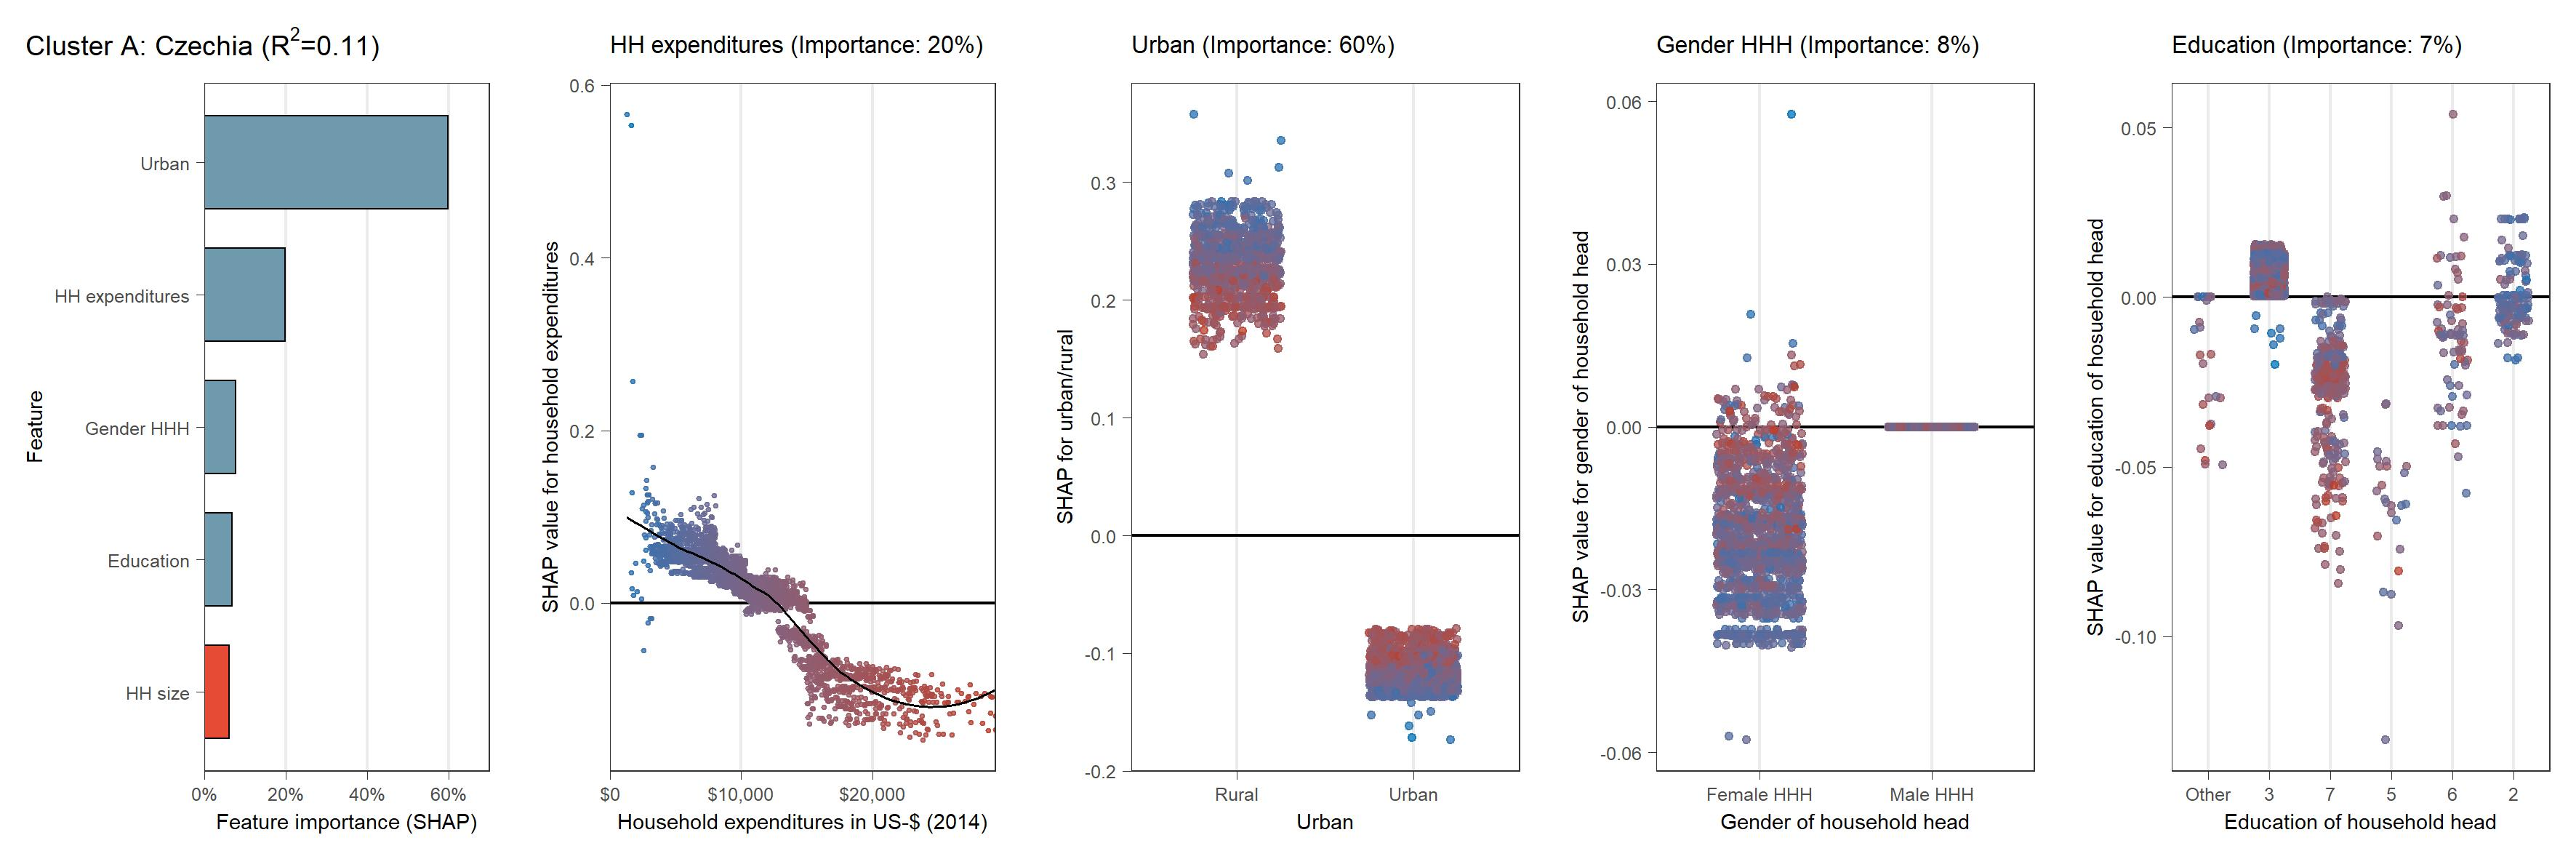
\includegraphics[width=\textwidth]{Figure 5b/Figure_5b_CZE}    \end{subfigure}
    \\
    \vspace{0.5cm}
   \begin{subfigure}[b]{\textwidth}
         \centering
         \caption{Partial dependence plot (SHAP) for Germany (cluster A)}
         \label{fig:5b_DEU}
         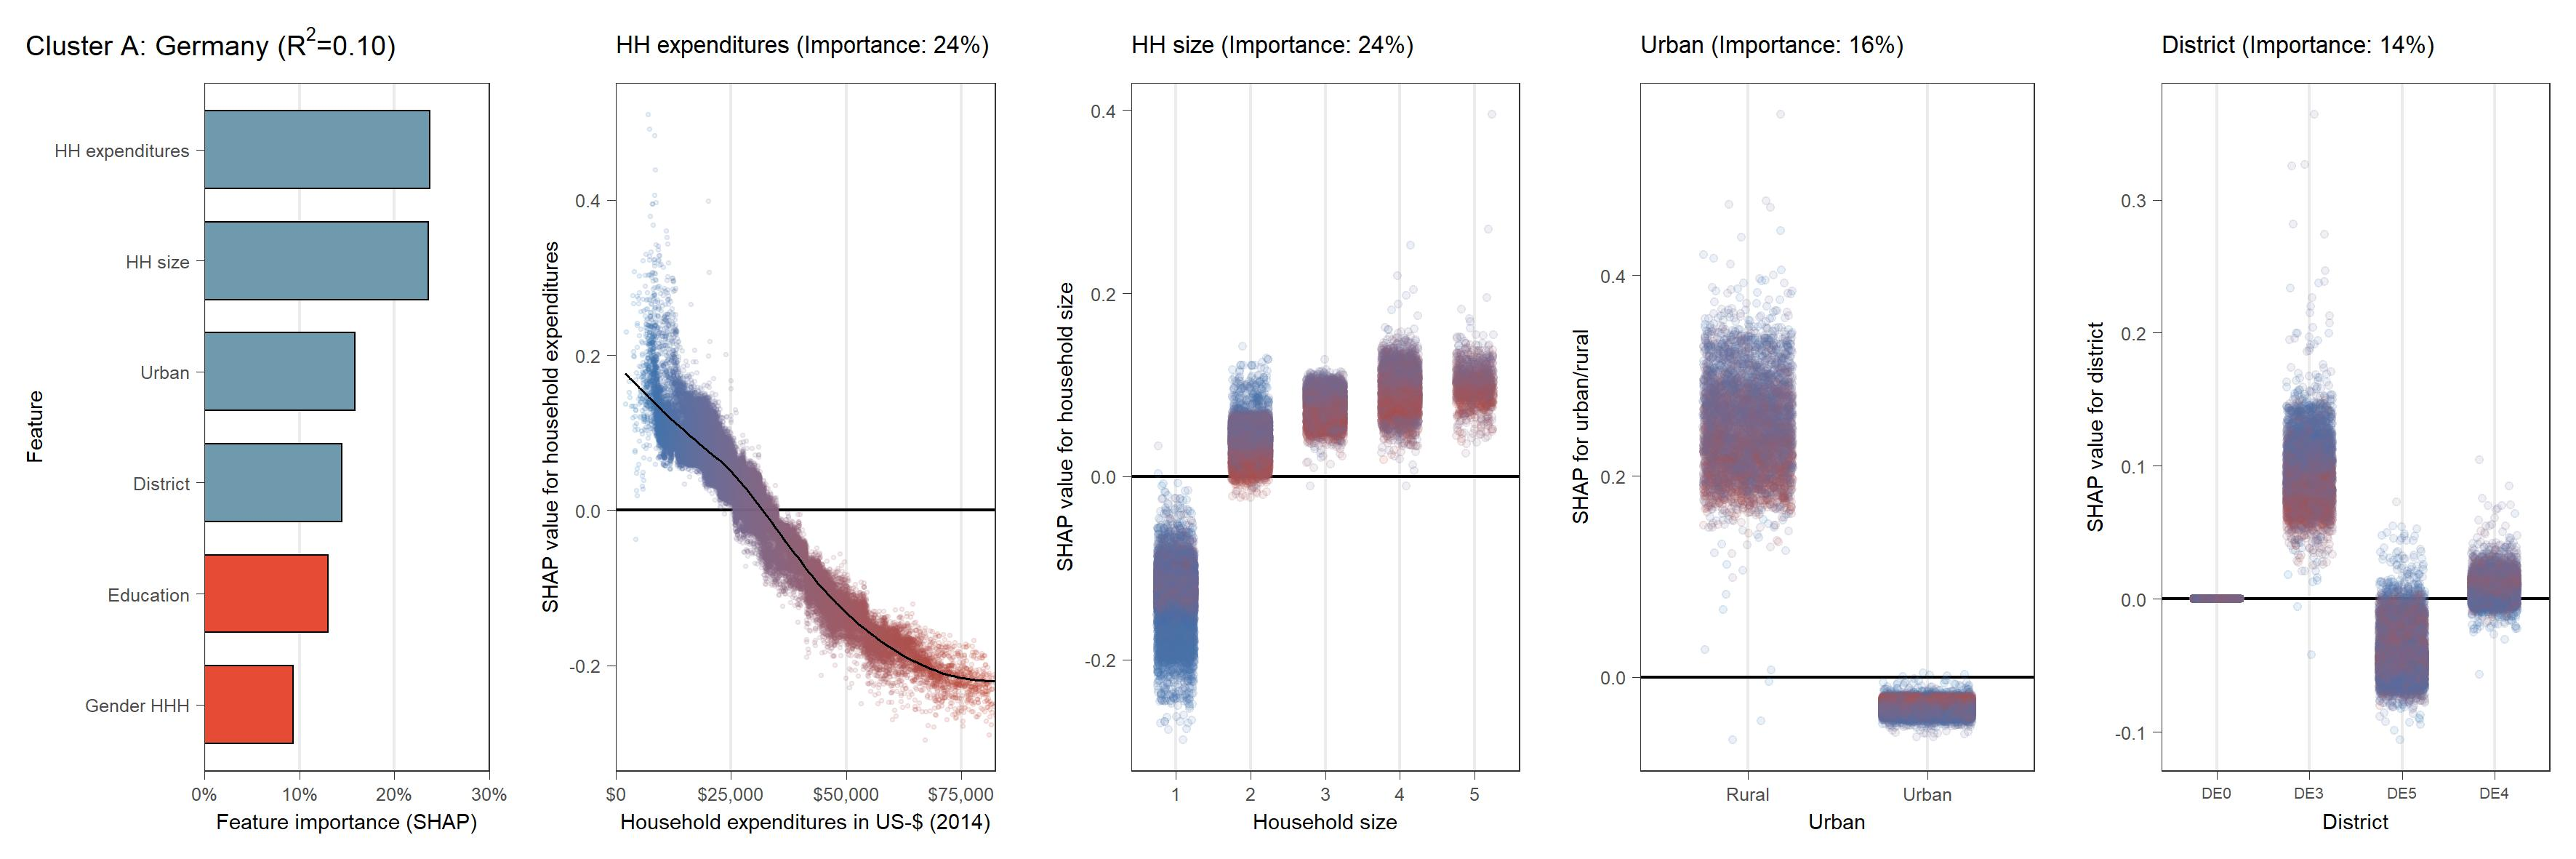
\includegraphics[width=\textwidth]{Figure 5b/Figure_5b_DEU}
         \end{subfigure}
    \\
    \vspace{0.5cm}
   \begin{subfigure}[b]{\textwidth}
         \centering
         \caption{Partial dependence plot (SHAP) for Denmark (cluster A)}
         \label{fig:5b_DNK}
         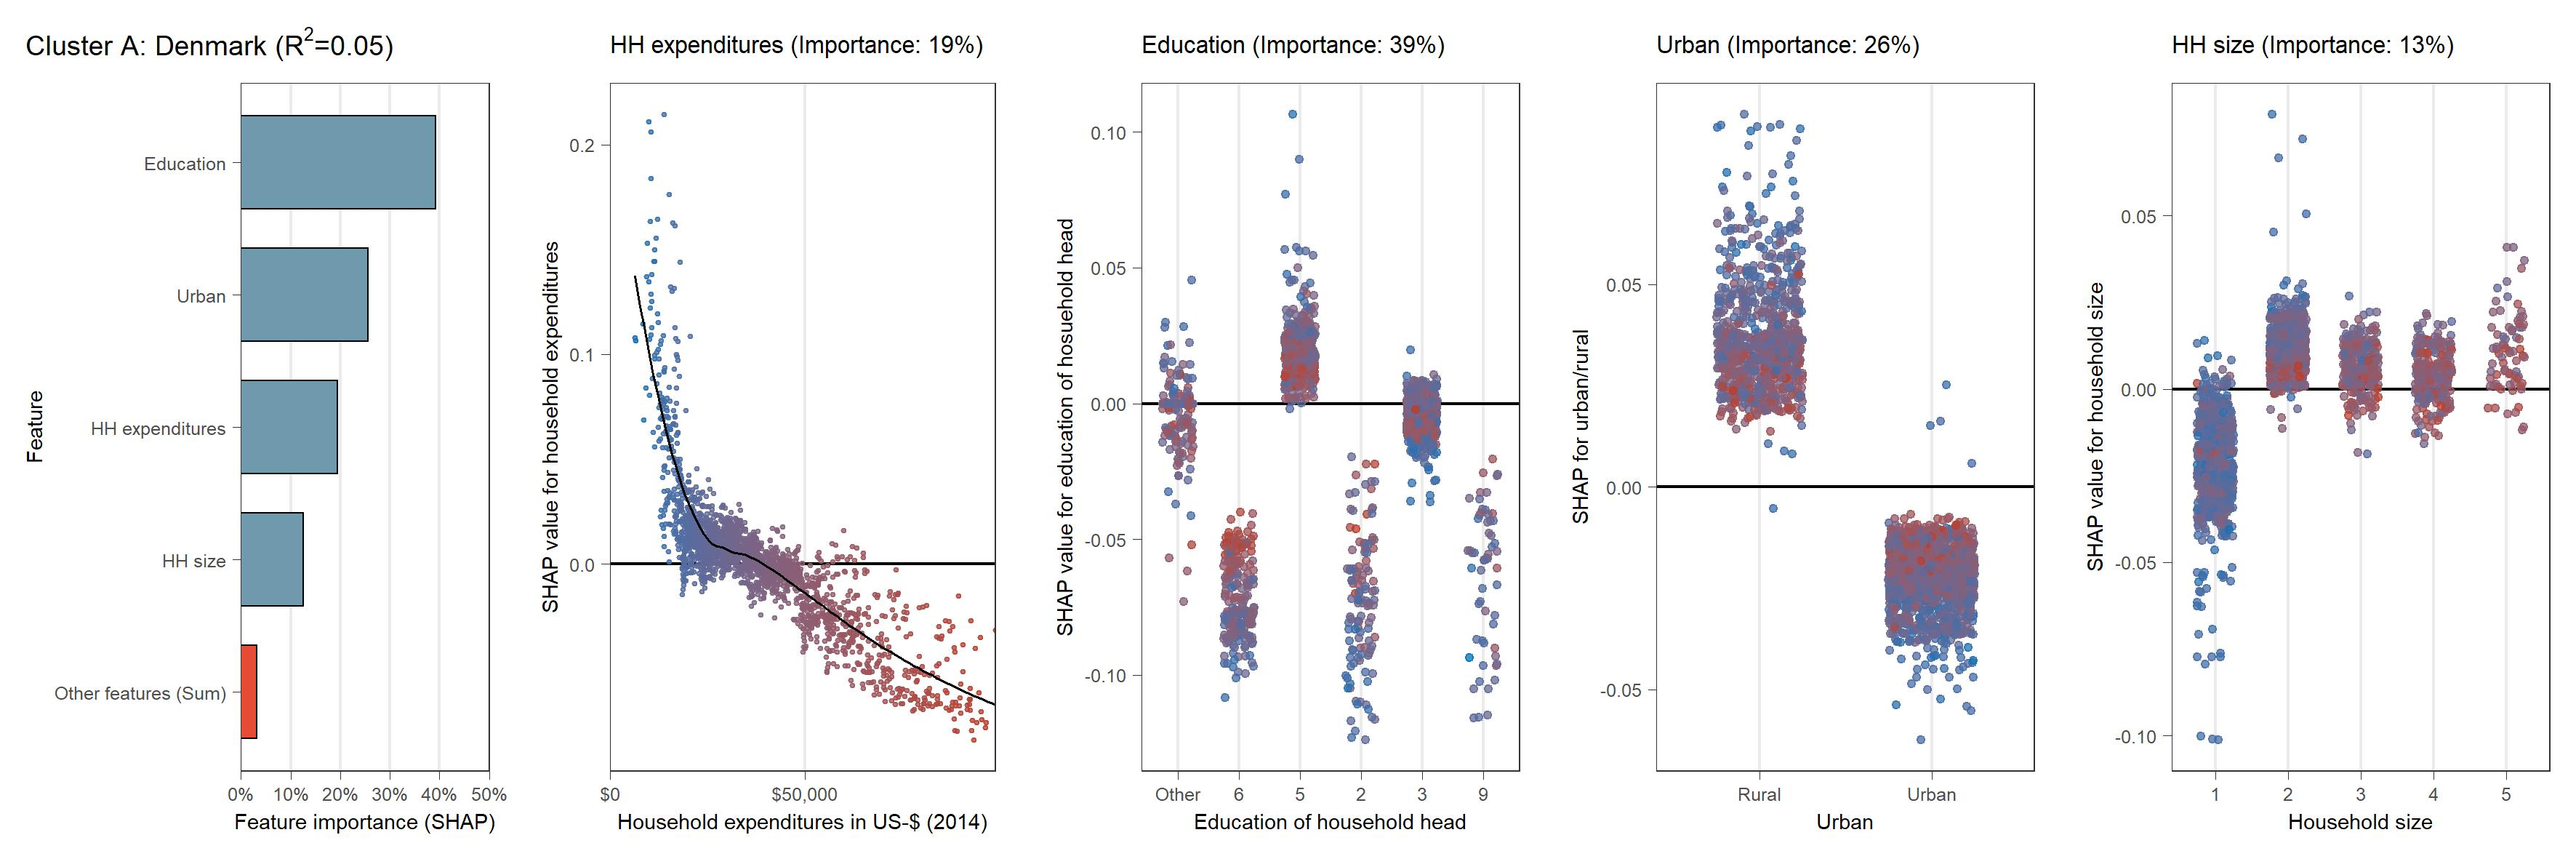
\includegraphics[width=\textwidth]{Figure 5b/Figure_5b_DNK} \end{subfigure}
    \\
    \vspace{0.5cm}
    \begin{subcaption2}
     This figure shows SHAP-values for predicting carbon intensity over feature values for 88 countries in alphabetical order for six country-clusters. The bar chart displays normalized average absolute SHAP-values for all features. Features with less than 3\% of normalized SHAP-values are subsumed as "Other features (Sum)". Panels show SHAP-values over total household expenditures for all countries and for the three most important features in each country besides total household expenditures. Colors represent household expenditures with blue (red) colors indicating lower (higher) household expenditures.
     \end{subcaption2}
\end{figure}

\begin{figure}[ht!]\ContinuedFloat
    \centering
   \begin{subfigure}[b]{\textwidth}
          \centering
         \caption{Partial dependence plot (SHAP) for Spain (cluster A)}
         \label{fig:5b_ESP}
         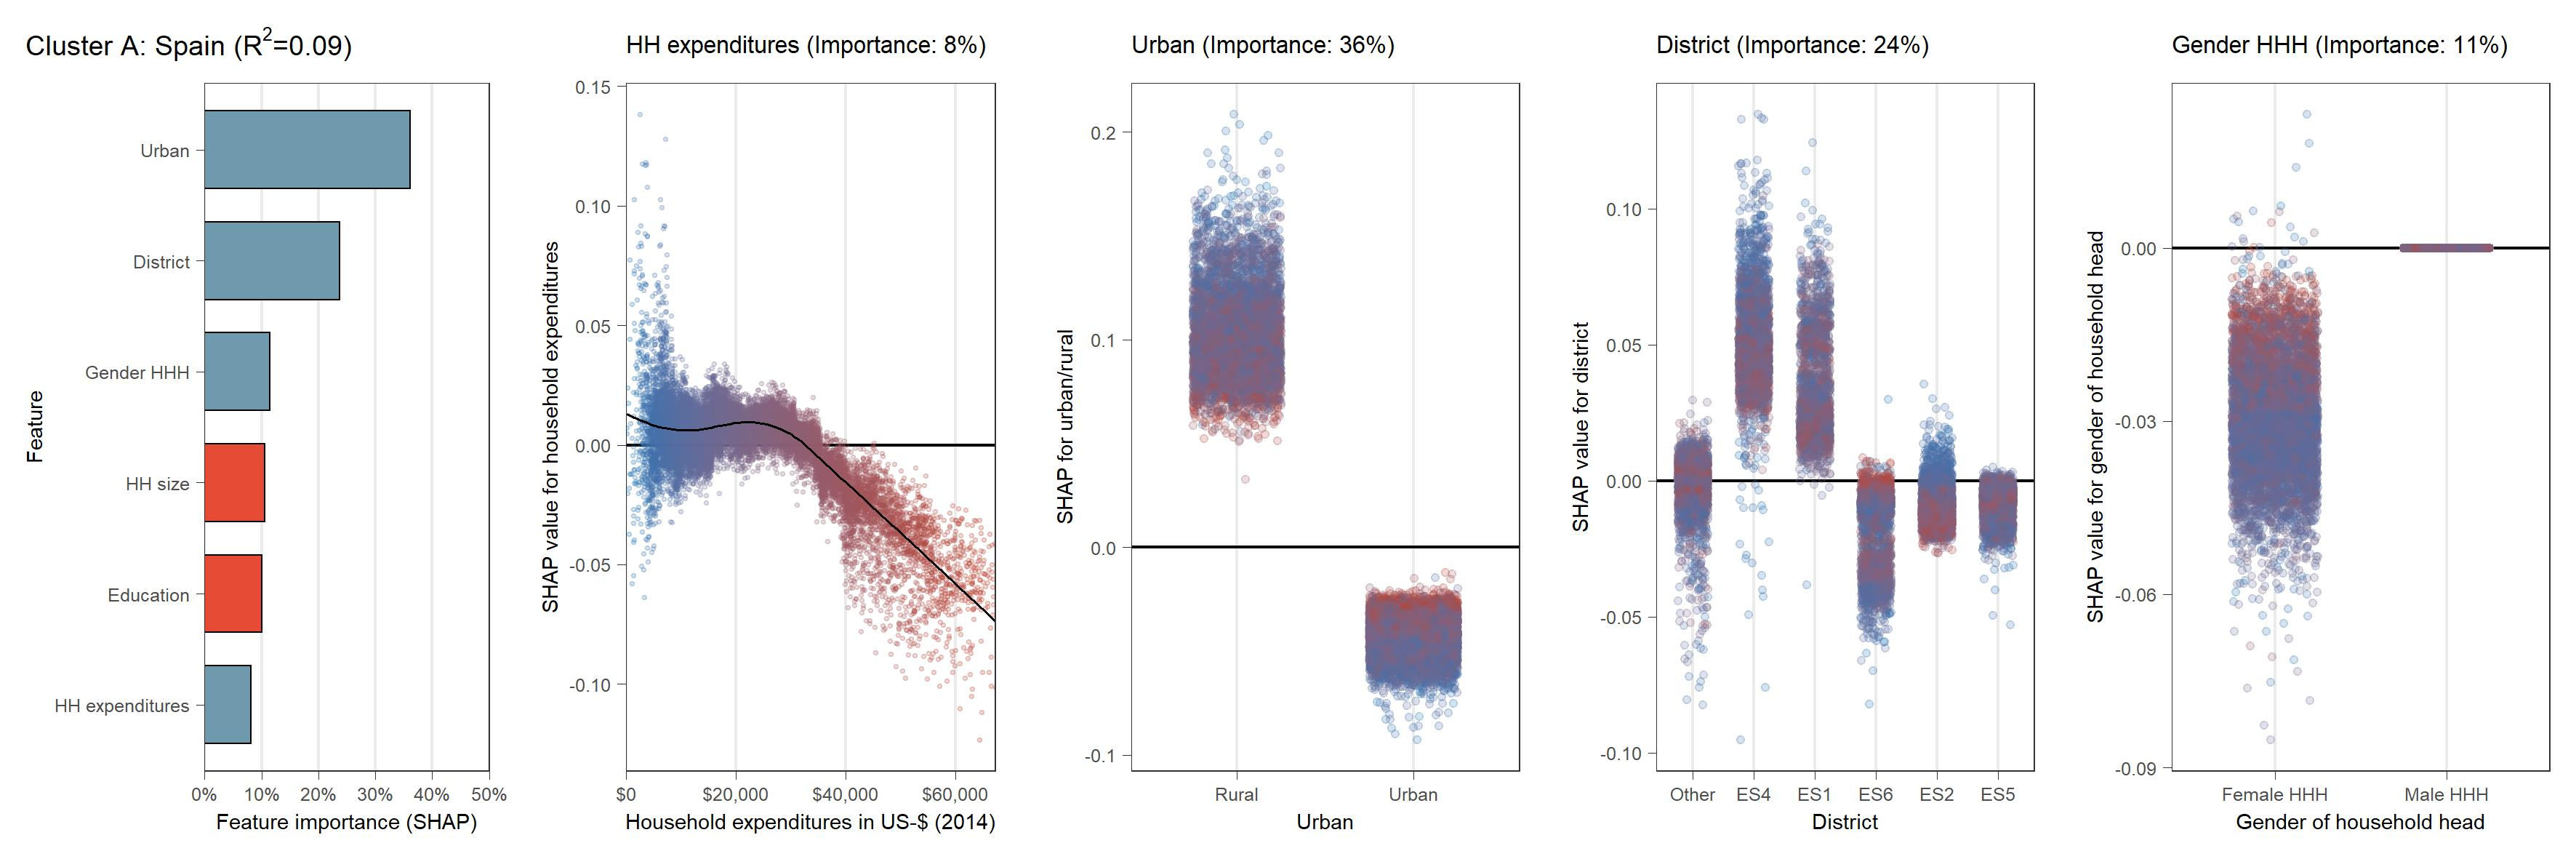
\includegraphics[width=\textwidth]{Figure 5b/Figure_5b_ESP}
     \end{subfigure}
    \\
    \vspace{0.5cm}
   \begin{subfigure}[b]{\textwidth}   
         \centering
         \caption{Partial dependence plot (SHAP) for Estonia (cluster A)}
         \label{fig:5b_EST}
         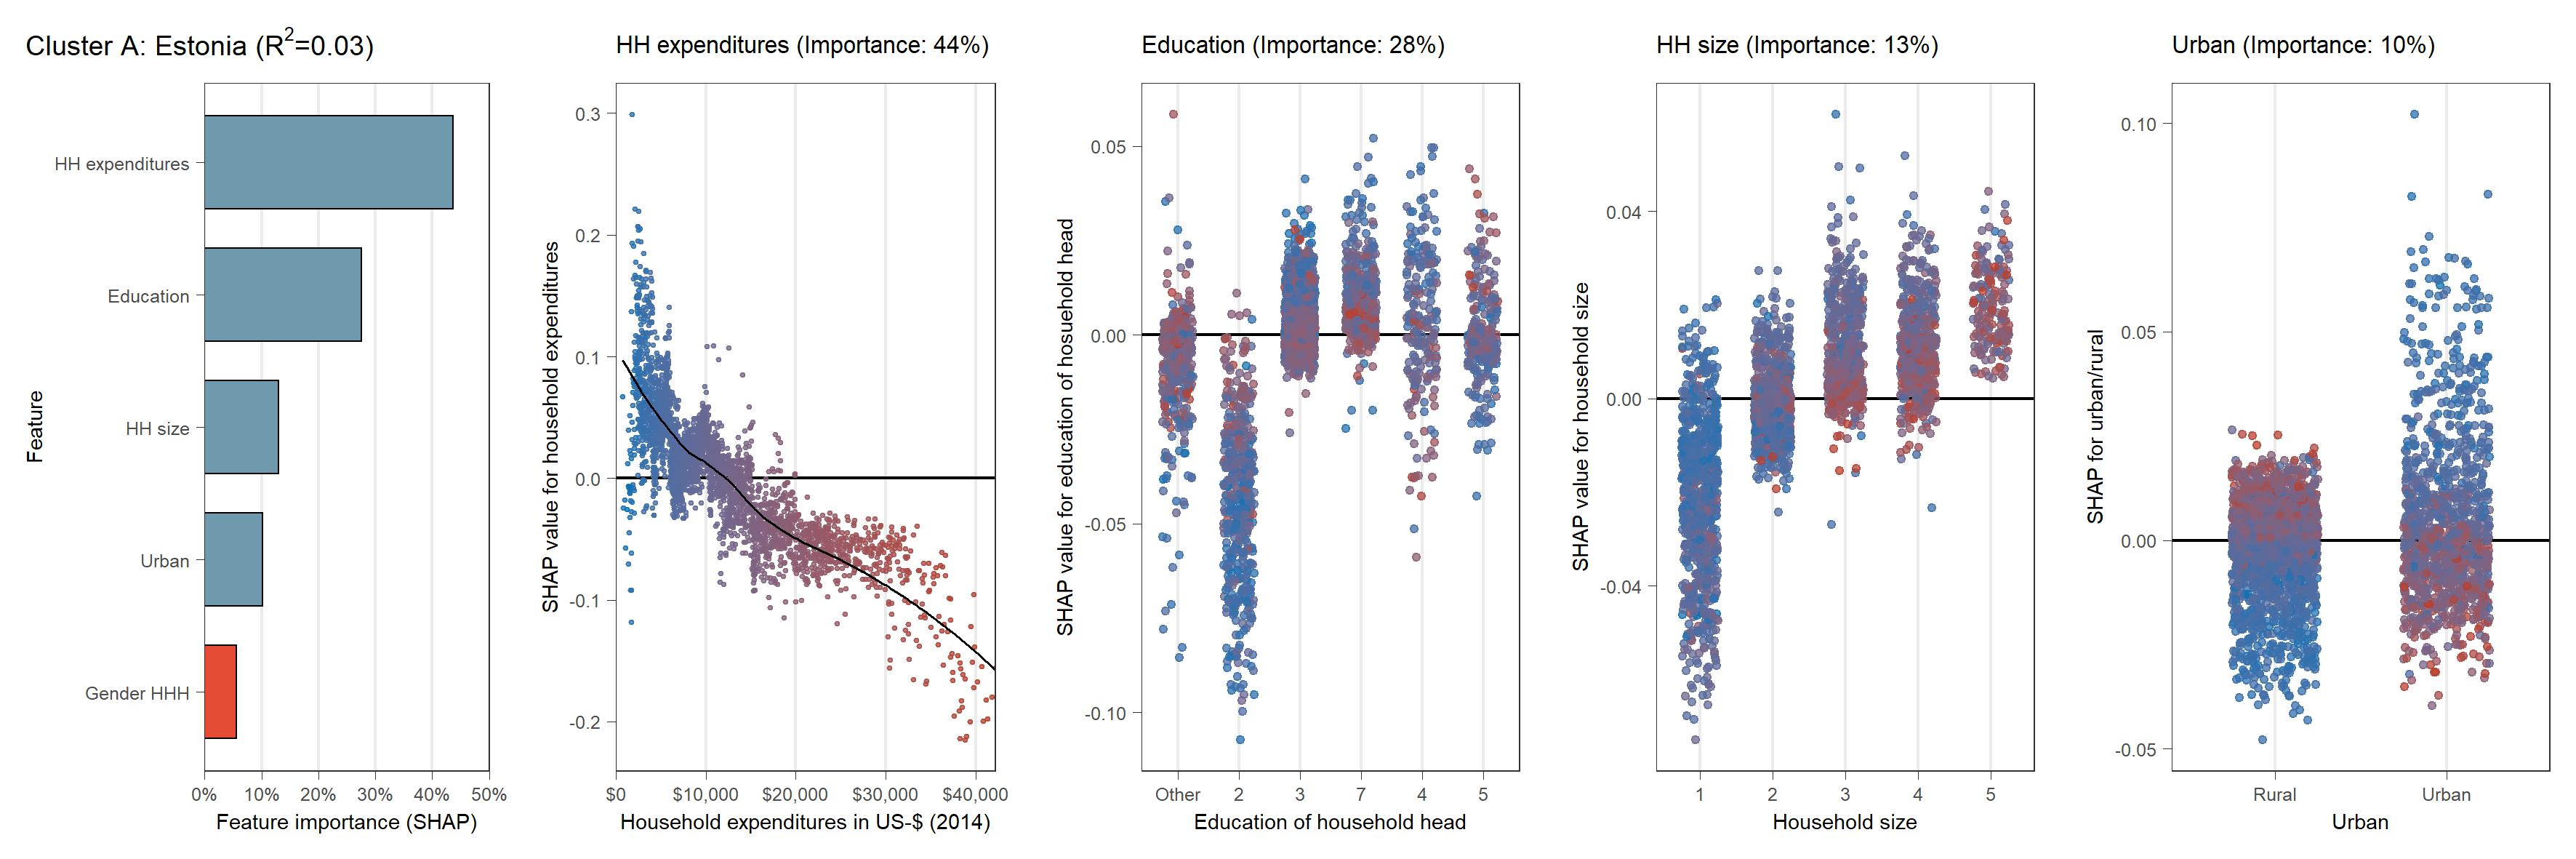
\includegraphics[width=\textwidth]{Figure 5b/Figure_5b_EST}
         \end{subfigure}
    \\
    \vspace{0.5cm}
   \begin{subfigure}[b]{\textwidth}
         \centering
         \caption{Partial dependence plot (SHAP) for Ethiopia (cluster A)}
         \label{fig:5b_ETH}
         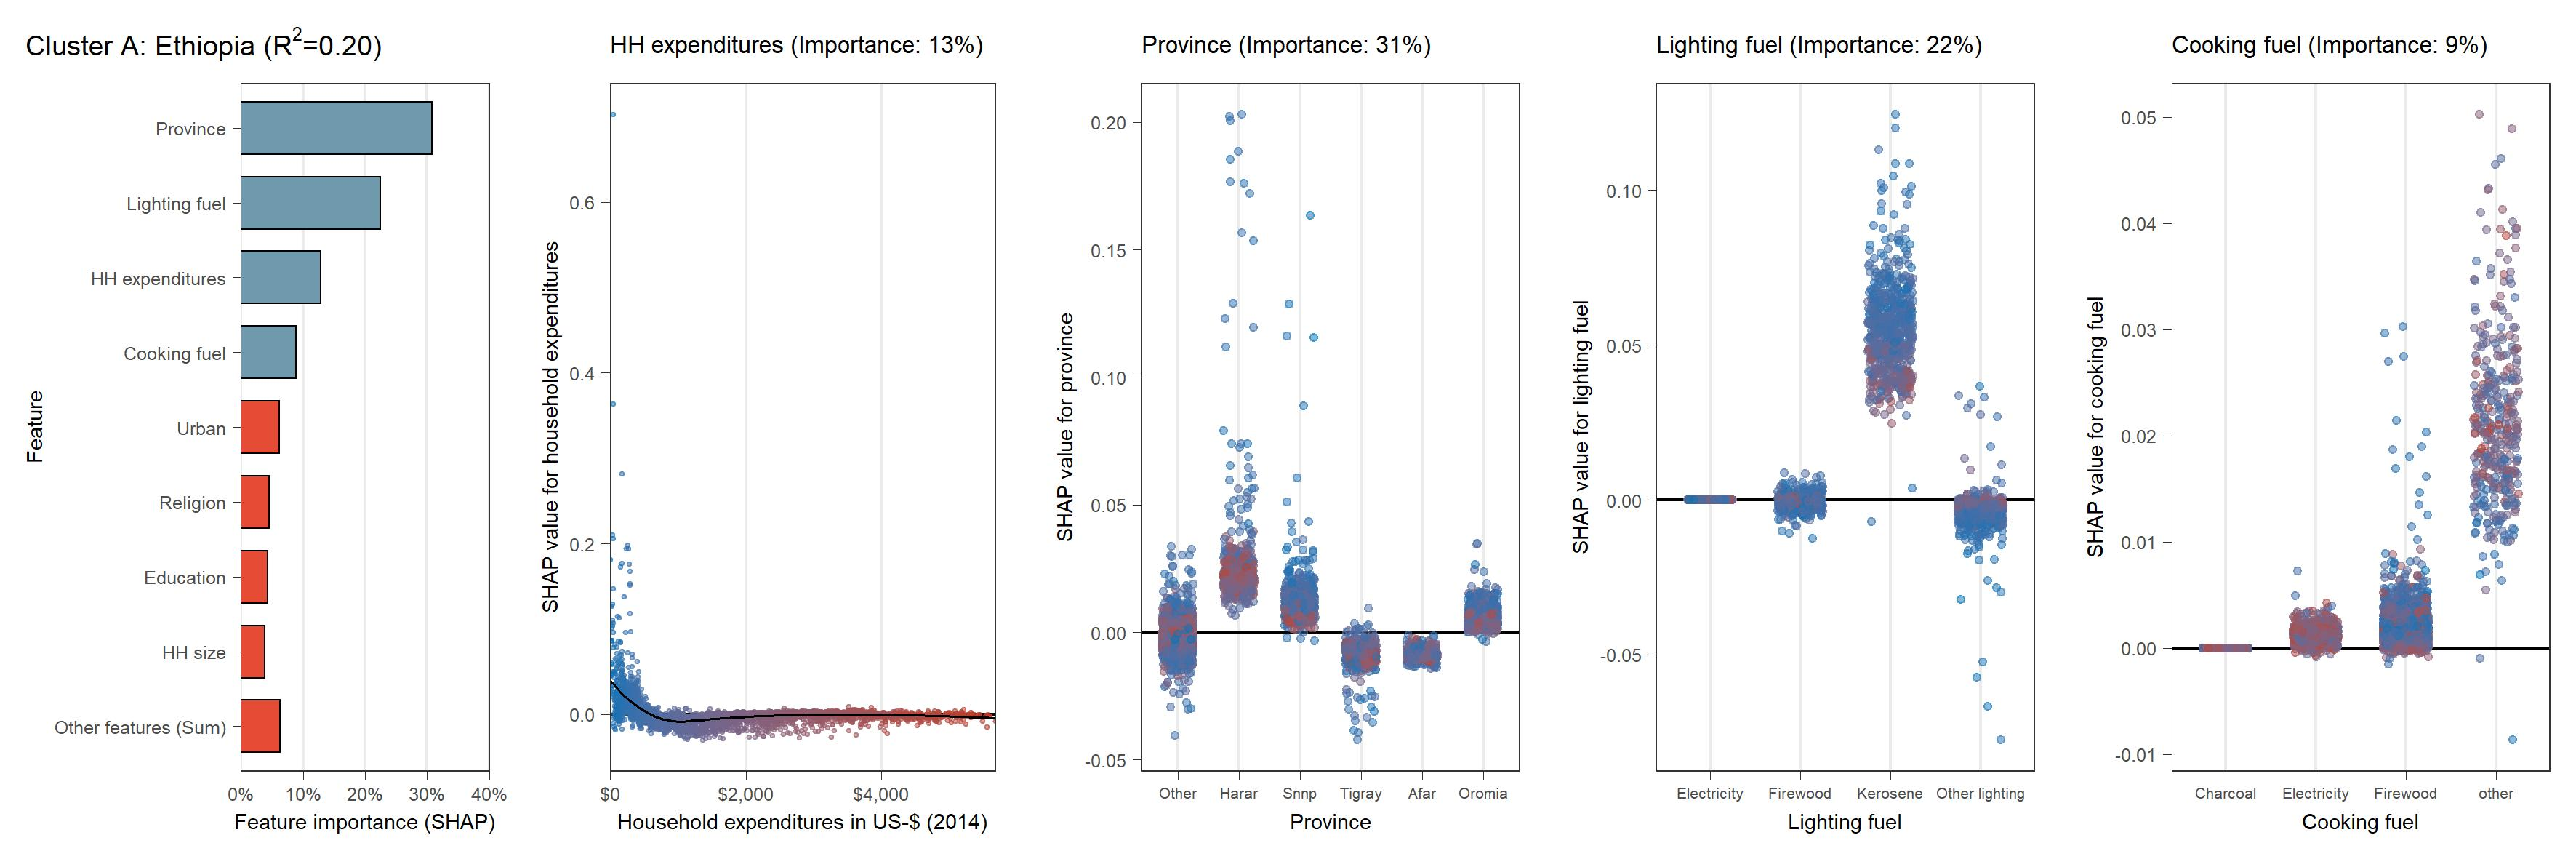
\includegraphics[width=\textwidth]{Figure 5b/Figure_5b_ETH} \end{subfigure}
    \\
    \vspace{0.5cm}
    \begin{subcaption2}
     This figure shows SHAP-values for predicting carbon intensity over feature values for 88 countries in alphabetical order for six country-clusters. The bar chart displays normalized average absolute SHAP-values for all features. Features with less than 3\% of normalized SHAP-values are subsumed as "Other features (Sum)". Panels show SHAP-values over total household expenditures for all countries and for the three most important features in each country besides total household expenditures. Colors represent household expenditures with blue (red) colors indicating lower (higher) household expenditures.
     \end{subcaption2}
\end{figure}

\begin{figure}[ht!]\ContinuedFloat
    \centering
   \begin{subfigure}[b]{\textwidth}
         \centering
         \caption{Partial dependence plot (SHAP) for Finland (cluster A)}
         \label{fig:5b_FIN}
         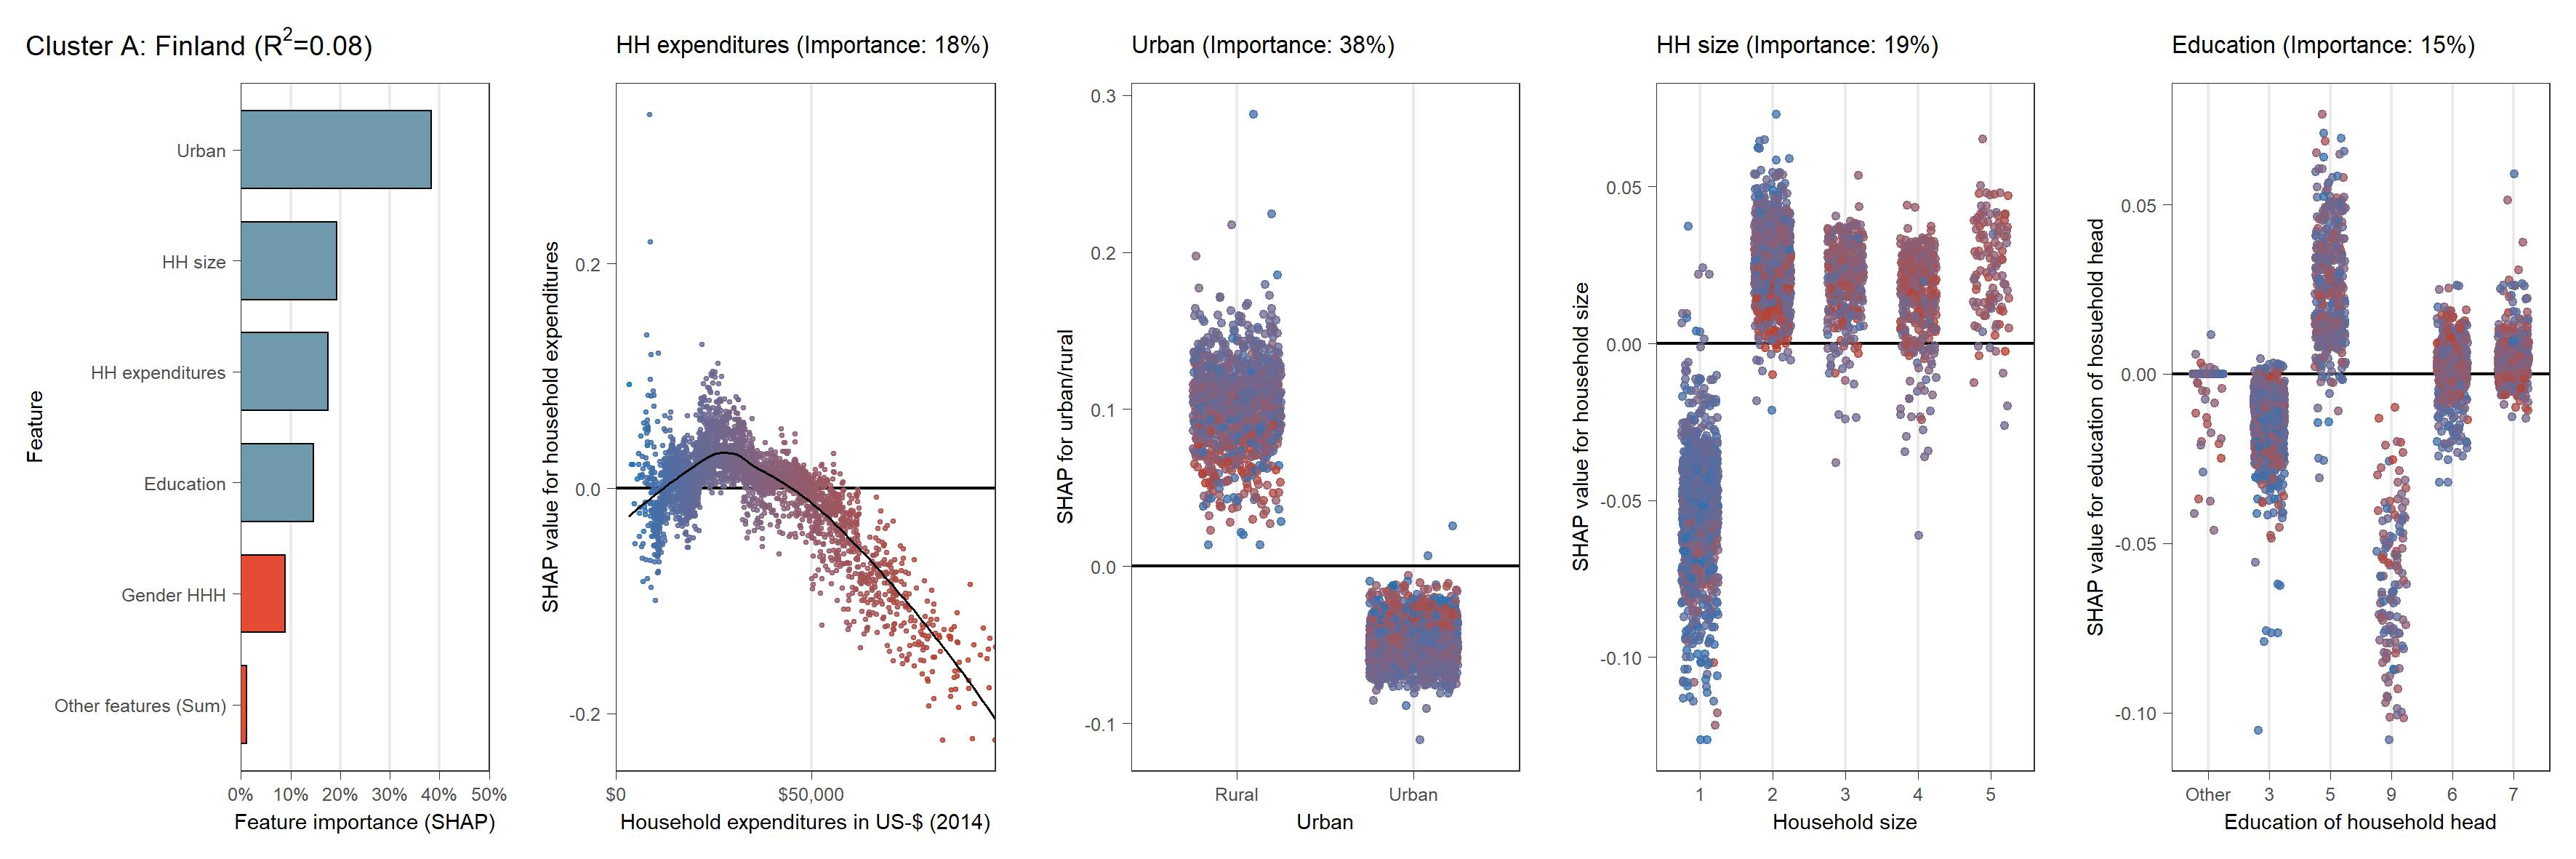
\includegraphics[width=\textwidth]{Figure 5b/Figure_5b_FIN}    
     \end{subfigure}
    \\
    \vspace{0.5cm}
   \begin{subfigure}[b]{\textwidth}
         \centering
         \caption{Partial dependence plot (SHAP) for France (cluster A)}
         \label{fig:5b_FRA}
         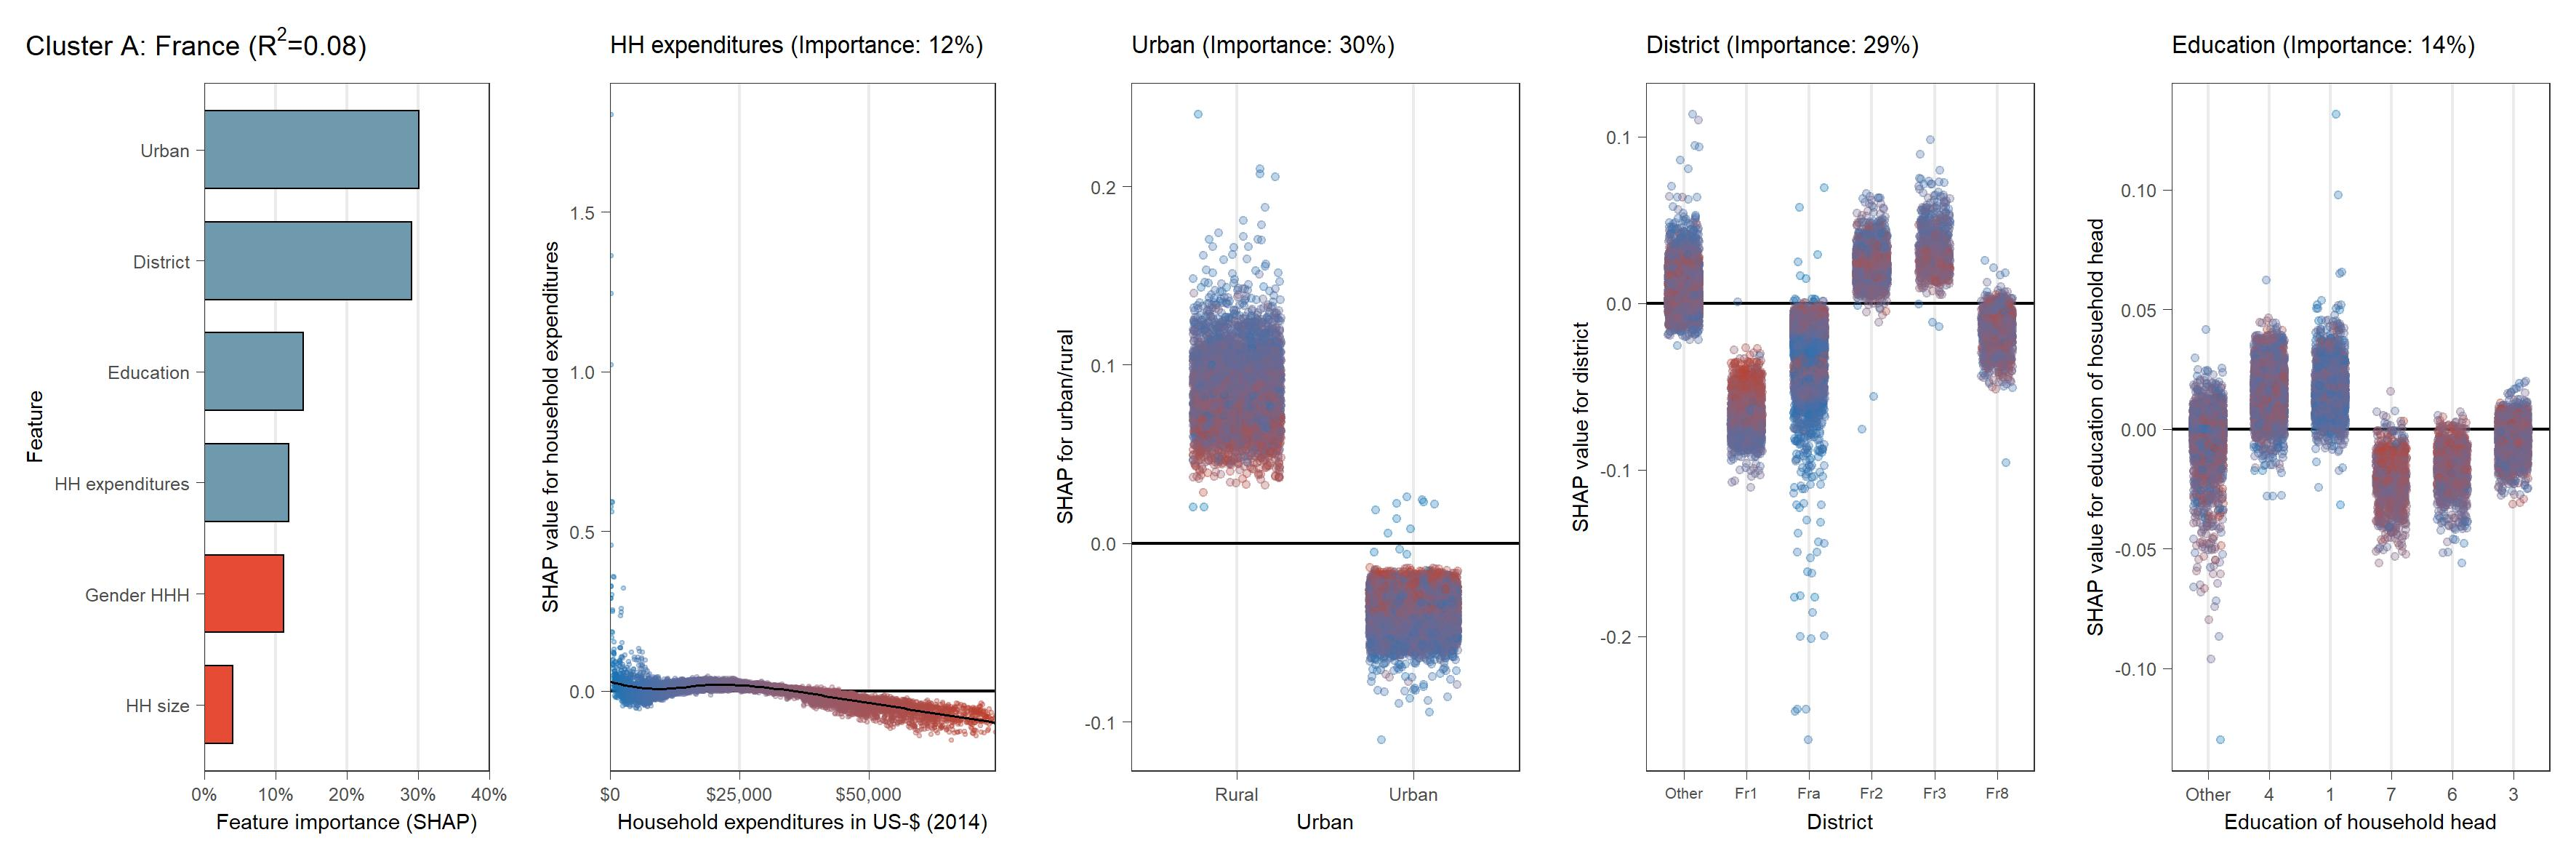
\includegraphics[width=\textwidth]{Figure 5b/Figure_5b_FRA} \end{subfigure}
    \\
    \vspace{0.5cm}
   \begin{subfigure}[b]{\textwidth}
         \centering
         \caption{Partial dependence plot (SHAP) for United Kingdom (cluster A)}
         \label{fig:5b_GBR}
         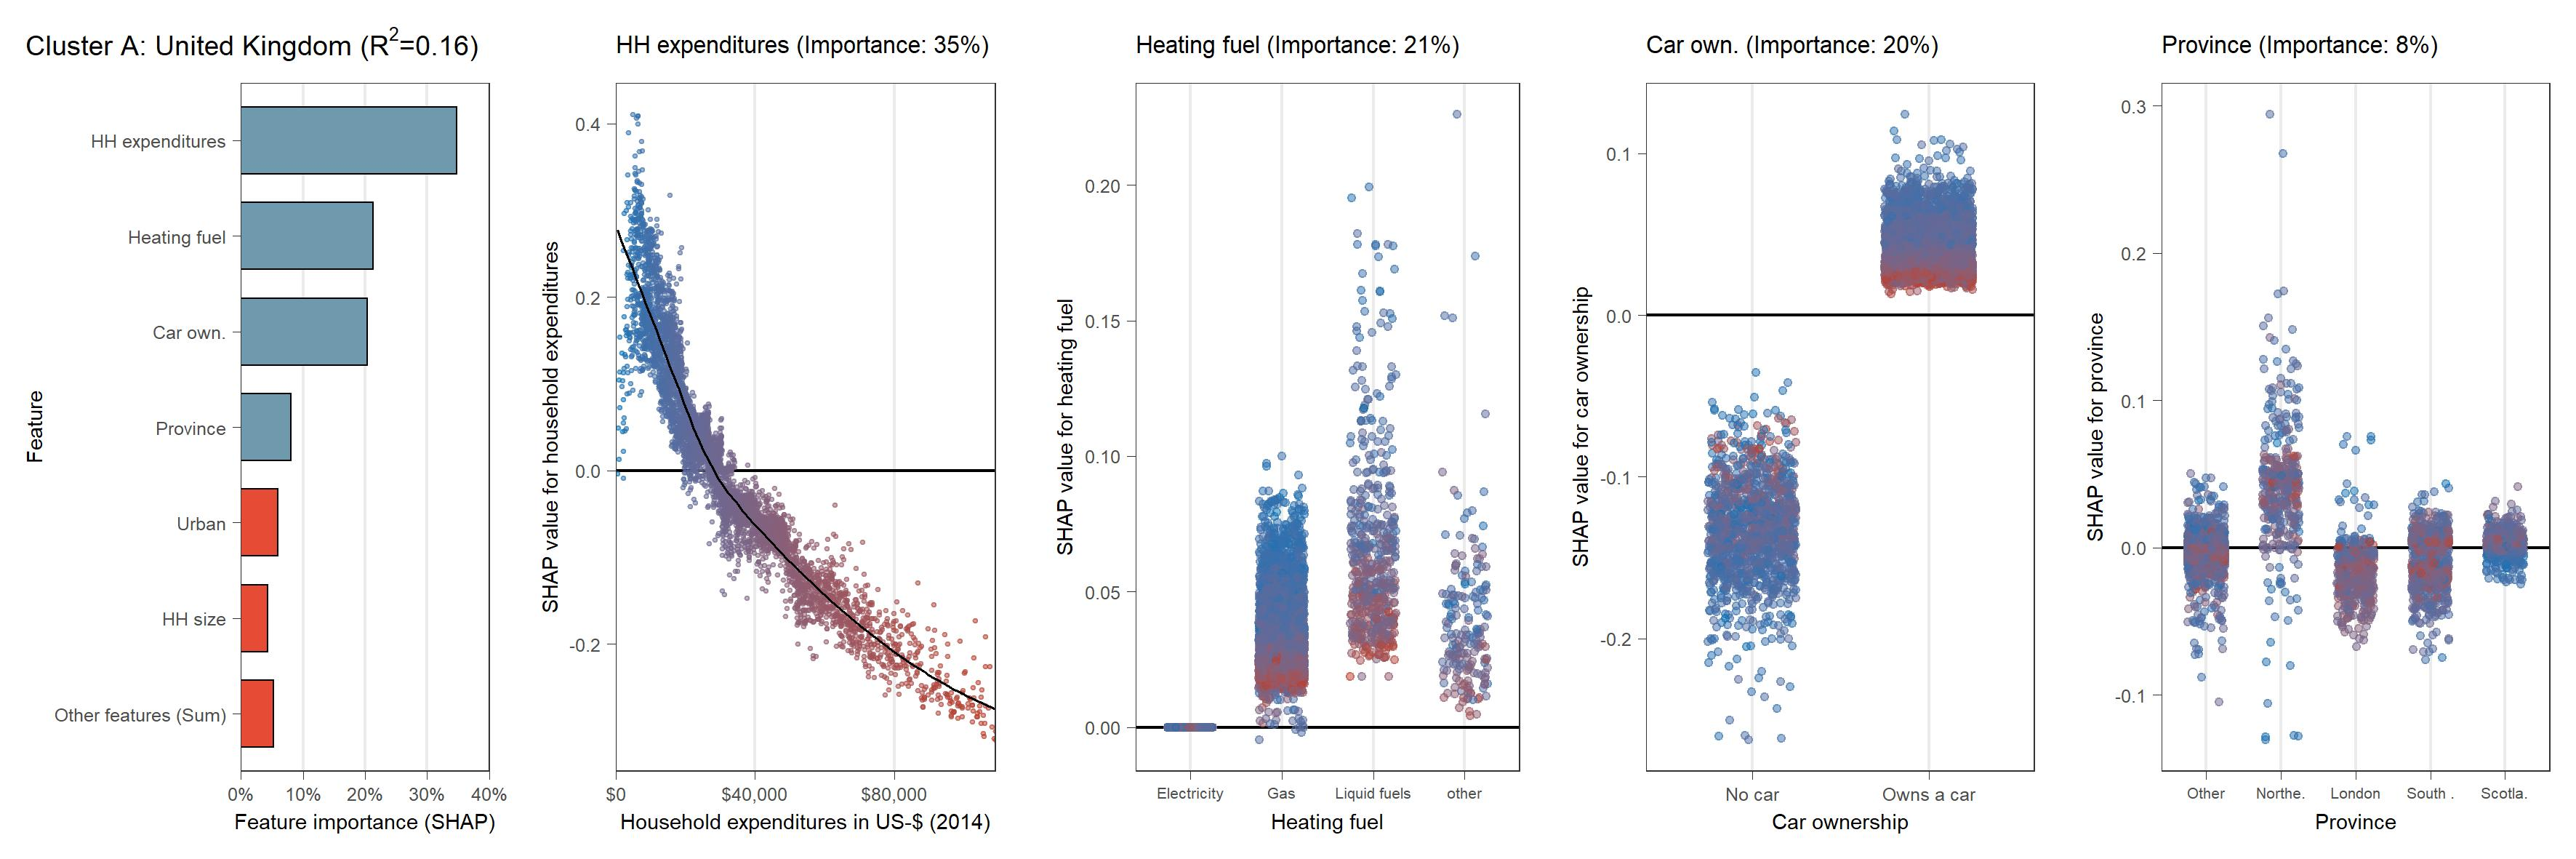
\includegraphics[width=\textwidth]{Figure 5b/Figure_5b_GBR}
    \end{subfigure}
    \\
    \vspace{0.5cm}
    \begin{subcaption2}
     This figure shows SHAP-values for predicting carbon intensity over feature values for 88 countries in alphabetical order for six country-clusters. The bar chart displays normalized average absolute SHAP-values for all features. Features with less than 3\% of normalized SHAP-values are subsumed as "Other features (Sum)". Panels show SHAP-values over total household expenditures for all countries and for the three most important features in each country besides total household expenditures. Colors represent household expenditures with blue (red) colors indicating lower (higher) household expenditures.
     \end{subcaption2}
\end{figure}

\begin{figure}[ht!]\ContinuedFloat
    \centering
   \begin{subfigure}[b]{\textwidth}
   \centering
         \caption{Partial dependence plot (SHAP) for Guinea-Bissau (cluster A)}
         \label{fig:5b_GNB}
         \includegraphics[width=\textwidth]{Figure 5b/Figure_5b_GNB}
         \end{subfigure}
    \\
    \vspace{0.5cm}
    \begin{subfigure}[b]{\textwidth}
   \centering
         \caption{Partial dependence plot (SHAP) for Greece (cluster A)}
         \label{fig:5b_GRC}
         \includegraphics[width=\textwidth]{Figure 5b/Figure_5b_GRC}
         \end{subfigure}
    \\
    \vspace{0.5cm}
   \begin{subfigure}[b]{\textwidth}
   \centering
         \caption{Partial dependence plot (SHAP) for Croatia (cluster A)}
         \label{fig:5b_HRV}
         \includegraphics[width=\textwidth]{Figure 5b/Figure_5b_HRV}     
     \end{subfigure}
    \\
    \vspace{0.5cm}
   
    \begin{subcaption2}
     This figure shows SHAP-values for predicting carbon intensity over feature values for 88 countries in alphabetical order for six country-clusters. The bar chart displays normalized average absolute SHAP-values for all features. Features with less than 3\% of normalized SHAP-values are subsumed as "Other features (Sum)". Panels show SHAP-values over total household expenditures for all countries and for the three most important features in each country besides total household expenditures. Colors represent household expenditures with blue (red) colors indicating lower (higher) household expenditures.
     \end{subcaption2}
\end{figure}

\begin{figure}[ht!]\ContinuedFloat
    \centering
   \begin{subfigure}[b]{\textwidth}
     \centering
         \caption{Partial dependence plot (SHAP) for Hungary (cluster A)}
         \label{fig:5b_HUN}
         \includegraphics[width=\textwidth]{Figure 5b/Figure_5b_HUN}
    \end{subfigure}
    \\
    \vspace{0.5cm}
    \begin{subfigure}[b]{\textwidth}
      \centering
         \caption{Partial dependence plot (SHAP) for Ireland (cluster A)}
         \label{fig:5b_IRL}
         \includegraphics[width=\textwidth]{Figure 5b/Figure_5b_IRL}   
     \end{subfigure}
    \\
    \vspace{0.5cm}
   \begin{subfigure}[b]{\textwidth}
   \centering
         \caption{Partial dependence plot (SHAP) for Israel (cluster A)}
         \label{fig:5b_ISR}
         \includegraphics[width=\textwidth]{Figure 5b/Figure_5b_ISR}
         \end{subfigure}
    \\
    \vspace{0.5cm}
   
    \begin{subcaption2}
     This figure shows SHAP-values for predicting carbon intensity over feature values for 88 countries in alphabetical order for six country-clusters. The bar chart displays normalized average absolute SHAP-values for all features. Features with less than 3\% of normalized SHAP-values are subsumed as "Other features (Sum)". Panels show SHAP-values over total household expenditures for all countries and for the three most important features in each country besides total household expenditures. Colors represent household expenditures with blue (red) colors indicating lower (higher) household expenditures.
     \end{subcaption2}
\end{figure}

\begin{figure}[ht!]\ContinuedFloat
    \centering
   \begin{subfigure}[b]{\textwidth}
         \centering
         \caption{Partial dependence plot (SHAP) for Italy (cluster A)}
         \label{fig:5b_ITA}
         \includegraphics[width=\textwidth]{Figure 5b/Figure_5b_ITA}     
    \end{subfigure}
    \\
    \vspace{0.5cm}
    \begin{subfigure}[b]{\textwidth}
         \centering
         \caption{Partial dependence plot (SHAP) for Kenya (cluster A)}
         \label{fig:5b_KEN}
         \includegraphics[width=\textwidth]{Figure 5b/Figure_5b_KEN}     
         \end{subfigure}
    \\
    \vspace{0.5cm}
   \begin{subfigure}[b]{\textwidth}        
         \centering
         \caption{Partial dependence plot (SHAP) for Cambodia (cluster A)}
         \label{fig:5b_KHM}
         \includegraphics[width=\textwidth]{Figure 5b/Figure_5b_KHM}
         \end{subfigure}
    \\
    \vspace{0.5cm}
   
    \begin{subcaption2}
     This figure shows SHAP-values for predicting carbon intensity over feature values for 88 countries in alphabetical order for six country-clusters. The bar chart displays normalized average absolute SHAP-values for all features. Features with less than 3\% of normalized SHAP-values are subsumed as "Other features (Sum)". Panels show SHAP-values over total household expenditures for all countries and for the three most important features in each country besides total household expenditures. Colors represent household expenditures with blue (red) colors indicating lower (higher) household expenditures.
     \end{subcaption2}
\end{figure}

\begin{figure}[ht!]\ContinuedFloat
    \centering
   \begin{subfigure}[b]{\textwidth}      
         \centering
         \caption{Partial dependence plot (SHAP) for Liberia (cluster A)}
         \label{fig:5b_LBR}
         \includegraphics[width=\textwidth]{Figure 5b/Figure_5b_LBR} 
         \end{subfigure}
    \\
    \vspace{0.5cm}
    \begin{subfigure}[b]{\textwidth}
         \centering
         \caption{Partial dependence plot (SHAP) for Lithuania (cluster A)}
         \label{fig:5b_LTU}
         \includegraphics[width=\textwidth]{Figure 5b/Figure_5b_LTU}
         \end{subfigure}
    \\
    \vspace{0.5cm}
   \begin{subfigure}[b]{\textwidth}
   \centering
         \caption{Partial dependence plot (SHAP) for Luxemburg (cluster A)}
         \label{fig:5b_LUX}
         \includegraphics[width=\textwidth]{Figure 5b/Figure_5b_LUX}
         \end{subfigure}
    \\
    \vspace{0.5cm}
   
    \begin{subcaption2}
     This figure shows SHAP-values for predicting carbon intensity over feature values for 88 countries in alphabetical order for six country-clusters. The bar chart displays normalized average absolute SHAP-values for all features. Features with less than 3\% of normalized SHAP-values are subsumed as "Other features (Sum)". Panels show SHAP-values over total household expenditures for all countries and for the three most important features in each country besides total household expenditures. Colors represent household expenditures with blue (red) colors indicating lower (higher) household expenditures.
     \end{subcaption2}
\end{figure}

\begin{figure}[ht!]\ContinuedFloat
    \centering
   \begin{subfigure}[b]{\textwidth}
    \centering
         \caption{Partial dependence plot (SHAP) for Latvia (cluster A)}
         \label{fig:5b_LVA}
         \includegraphics[width=\textwidth]{Figure 5b/Figure_5b_LVA}     
         \end{subfigure}
    \\
    \vspace{0.5cm}
    \begin{subfigure}[b]{\textwidth}
    \centering
         \caption{Partial dependence plot (SHAP) for Morocco (cluster A)}
         \label{fig:5b_MAR}
         \includegraphics[width=\textwidth]{Figure 5b/Figure_5b_MAR}     
     \end{subfigure}
    \\
    \vspace{0.5cm}
   \begin{subfigure}[b]{\textwidth}
    \centering
         \caption{Partial dependence plot (SHAP) for Maldives (cluster A)}
         \label{fig:5b_MDV}
         \includegraphics[width=\textwidth]{Figure 5b/Figure_5b_MDV}     
         \end{subfigure}
    \\
    \vspace{0.5cm}
   
    \begin{subcaption2}
     This figure shows SHAP-values for predicting carbon intensity over feature values for 88 countries in alphabetical order for six country-clusters. The bar chart displays normalized average absolute SHAP-values for all features. Features with less than 3\% of normalized SHAP-values are subsumed as "Other features (Sum)". Panels show SHAP-values over total household expenditures for all countries and for the three most important features in each country besides total household expenditures. Colors represent household expenditures with blue (red) colors indicating lower (higher) household expenditures.
     \end{subcaption2}
\end{figure}

\begin{figure}[ht!]\ContinuedFloat
    \centering
   \begin{subfigure}[b]{\textwidth}
   \centering
         \caption{Partial dependence plot (SHAP) for Myanmar (cluster A)}
         \label{fig:5b_MMR}
         \includegraphics[width=\textwidth]{Figure 5b/Figure_5b_MMR}     
         \end{subfigure}
    \\
    \vspace{0.5cm}
    \begin{subfigure}[b]{\textwidth}
   \centering
         \caption{Partial dependence plot (SHAP) for Mongolia (cluster A)}
         \label{fig:5b_MNG}
         \includegraphics[width=\textwidth]{Figure 5b/Figure_5b_MNG}
         \end{subfigure}
    \\
    \vspace{0.5cm}
   \begin{subfigure}[b]{\textwidth}         
         \centering
         \caption{Partial dependence plot (SHAP) for Mozambique (cluster A)}
         \label{fig:5b_MOZ}
         \includegraphics[width=\textwidth]{Figure 5b/Figure_5b_MOZ}
         \end{subfigure}
    \\
    \vspace{0.5cm}
   
    \begin{subcaption2}
     This figure shows SHAP-values for predicting carbon intensity over feature values for 88 countries in alphabetical order for six country-clusters. The bar chart displays normalized average absolute SHAP-values for all features. Features with less than 3\% of normalized SHAP-values are subsumed as "Other features (Sum)". Panels show SHAP-values over total household expenditures for all countries and for the three most important features in each country besides total household expenditures. Colors represent household expenditures with blue (red) colors indicating lower (higher) household expenditures.
     \end{subcaption2}
\end{figure}

\begin{figure}[ht!]\ContinuedFloat
    \centering
   \begin{subfigure}[b]{\textwidth}
   \centering
         \caption{Partial dependence plot (SHAP) for Malawi (cluster A)}
         \label{fig:5b_MWI}
         \includegraphics[width=\textwidth]{Figure 5b/Figure_5b_MWI}
         \end{subfigure}
    \\
    \vspace{0.5cm}
    \begin{subfigure}[b]{\textwidth}
    \centering
         \caption{Partial dependence plot (SHAP) for the Netherlands (cluster A)}
         \label{fig:5b_NLD}
         \includegraphics[width=\textwidth]{Figure 5b/Figure_5b_NLD}
         \end{subfigure}
    \\
    \vspace{0.5cm}
   \begin{subfigure}[b]{\textwidth}
   \centering
         \caption{Partial dependence plot (SHAP) for Norway (cluster A)}
         \label{fig:5b_NOR}
         \includegraphics[width=\textwidth]{Figure 5b/Figure_5b_NOR} 
         \end{subfigure}
    \\
    \vspace{0.5cm}
   
    \begin{subcaption2}
     This figure shows SHAP-values for predicting carbon intensity over feature values for 88 countries in alphabetical order for six country-clusters. The bar chart displays normalized average absolute SHAP-values for all features. Features with less than 3\% of normalized SHAP-values are subsumed as "Other features (Sum)". Panels show SHAP-values over total household expenditures for all countries and for the three most important features in each country besides total household expenditures. Colors represent household expenditures with blue (red) colors indicating lower (higher) household expenditures.
     \end{subcaption2}
\end{figure}

\begin{figure}[ht!]\ContinuedFloat
    \centering
   \begin{subfigure}[b]{\textwidth}
   \centering
         \caption{Partial dependence plot (SHAP) for Poland (cluster A)}
         \label{fig:5b_POL}
         \includegraphics[width=\textwidth]{Figure 5b/Figure_5b_POL}         
     \end{subfigure}
    \\
    \vspace{0.5cm}
    \begin{subfigure}[b]{\textwidth}
   \centering
         \caption{Partial dependence plot (SHAP) for Portugal (cluster A)}
         \label{fig:5b_PRT}
         \includegraphics[width=\textwidth]{Figure 5b/Figure_5b_PRT}
         \end{subfigure}
    \\
    \vspace{0.5cm}
   \begin{subfigure}[b]{\textwidth}
         \centering
         \caption{Partial dependence plot (SHAP) for Romania (cluster A)}
         \label{fig:5b_ROU}
         \includegraphics[width=\textwidth]{Figure 5b/Figure_5b_ROU}
         \end{subfigure}
    \\
    \vspace{0.5cm}
   
    \begin{subcaption2}
     This figure shows SHAP-values for predicting carbon intensity over feature values for 88 countries in alphabetical order for six country-clusters. The bar chart displays normalized average absolute SHAP-values for all features. Features with less than 3\% of normalized SHAP-values are subsumed as "Other features (Sum)". Panels show SHAP-values over total household expenditures for all countries and for the three most important features in each country besides total household expenditures. Colors represent household expenditures with blue (red) colors indicating lower (higher) household expenditures.
     \end{subcaption2}
\end{figure}

\begin{figure}[ht!]\ContinuedFloat
    \centering
   \begin{subfigure}[b]{\textwidth}
    \centering
         \caption{Partial dependence plot (SHAP) for Serbia (cluster A)}
         \label{fig:5b_SRB}
         \includegraphics[width=\textwidth]{Figure 5b/Figure_5b_SRB}
         \end{subfigure}
    \\
    \vspace{0.5cm}
    \begin{subfigure}[b]{\textwidth}
   \centering
         \caption{Partial dependence plot (SHAP) for Suriname (cluster A)}
         \label{fig:5b_SUR}
         \includegraphics[width=\textwidth]{Figure 5b/Figure_5b_SUR}
         \end{subfigure}
    \\
    \vspace{0.5cm}
   \begin{subfigure}[b]{\textwidth}
         \centering
         \caption{Partial dependence plot (SHAP) for Slovakia (cluster A)}
         \label{fig:5b_SVK}
         \includegraphics[width=\textwidth]{Figure 5b/Figure_5b_SVK}
         \end{subfigure}
    \\
    \vspace{0.5cm}
   
    \begin{subcaption2}
     This figure shows SHAP-values for predicting carbon intensity over feature values for 88 countries in alphabetical order for six country-clusters. The bar chart displays normalized average absolute SHAP-values for all features. Features with less than 3\% of normalized SHAP-values are subsumed as "Other features (Sum)". Panels show SHAP-values over total household expenditures for all countries and for the three most important features in each country besides total household expenditures. Colors represent household expenditures with blue (red) colors indicating lower (higher) household expenditures.
     \end{subcaption2}
\end{figure}

\begin{figure}[ht!]\ContinuedFloat
    \centering
   \begin{subfigure}[b]{\textwidth}
    \centering
         \caption{Partial dependence plot (SHAP) for Sweden (cluster A)}
         \label{fig:5b_SWE}
         \includegraphics[width=\textwidth]{Figure 5b/Figure_5b_SWE}
         \end{subfigure}
    \\
    \vspace{0.5cm}
    \begin{subfigure}[b]{\textwidth}
   \centering
         \caption{Partial dependence plot (SHAP) for USA (cluster A)}
         \label{fig:5b_USA}
         \includegraphics[width=\textwidth]{Figure 5b/Figure_5b_USA}   
         \end{subfigure}
    \\
    \vspace{0.5cm}
   \begin{subfigure}[b]{\textwidth}
         \centering
         \caption{Partial dependence plot (SHAP) for Barbados (cluster B)}
         \label{fig:5b_BRB}
         \includegraphics[width=\textwidth]{Figure 5b/Figure_5b_BRB}
         \end{subfigure}
    \\
    \vspace{0.5cm}
   
    \begin{subcaption2}
     This figure shows SHAP-values for predicting carbon intensity over feature values for 88 countries in alphabetical order for six country-clusters. The bar chart displays normalized average absolute SHAP-values for all features. Features with less than 3\% of normalized SHAP-values are subsumed as "Other features (Sum)". Panels show SHAP-values over total household expenditures for all countries and for the three most important features in each country besides total household expenditures. Colors represent household expenditures with blue (red) colors indicating lower (higher) household expenditures.
     \end{subcaption2}
\end{figure}

\begin{figure}[ht!]\ContinuedFloat
    \centering
   \begin{subfigure}[b]{\textwidth}
   \centering
         \caption{Partial dependence plot (SHAP) for Costa Rica (cluster B)}
         \label{fig:5b_CRI}
         \includegraphics[width=\textwidth]{Figure 5b/Figure_5b_CRI}
    \end{subfigure}
    \\
    \vspace{0.5cm}
    \begin{subfigure}[b]{\textwidth}
   \centering
         \caption{Partial dependence plot (SHAP) for Dominican Republic (cluster B)}
         \label{fig:5b_DOM}
         \includegraphics[width=\textwidth]{Figure 5b/Figure_5b_DOM} 
         \end{subfigure}
    \\
    \vspace{0.5cm}
   \begin{subfigure}[b]{\textwidth}        
   \centering
         \caption{Partial dependence plot (SHAP) for Egypt (cluster B)}
         \label{fig:5b_EGY}
         \includegraphics[width=\textwidth]{Figure 5b/Figure_5b_EGY}
         \end{subfigure}
    \\
    \vspace{0.5cm}
   
    \begin{subcaption2}
     This figure shows SHAP-values for predicting carbon intensity over feature values for 88 countries in alphabetical order for six country-clusters. The bar chart displays normalized average absolute SHAP-values for all features. Features with less than 3\% of normalized SHAP-values are subsumed as "Other features (Sum)". Panels show SHAP-values over total household expenditures for all countries and for the three most important features in each country besides total household expenditures. Colors represent household expenditures with blue (red) colors indicating lower (higher) household expenditures.
     \end{subcaption2}
\end{figure}

\begin{figure}[ht!]\ContinuedFloat
    \centering
   \begin{subfigure}[b]{\textwidth}
   \centering
         \caption{Partial dependence plot (SHAP) for Georgia (cluster B)}
         \label{fig:5b_GEO}
         \includegraphics[width=\textwidth]{Figure 5b/Figure_5b_GEO}
         \end{subfigure}
    \\
    \vspace{0.5cm}
    \begin{subfigure}[b]{\textwidth}
           \centering
         \caption{Partial dependence plot (SHAP) for Guatemala (cluster B)}
         \label{fig:5b_GTM}
         \includegraphics[width=\textwidth]{Figure 5b/Figure_5b_GTM}
         \end{subfigure}
    \\
    \vspace{0.5cm}
   \begin{subfigure}[b]{\textwidth}
   \centering
         \caption{Partial dependence plot (SHAP) for Indonesia (cluster B)}
         \label{fig:5b_IDN}
         \includegraphics[width=\textwidth]{Figure 5b/Figure_5b_IDN}
     \end{subfigure}
    \\
    \vspace{0.5cm}
  
    \begin{subcaption2}
     This figure shows SHAP-values for predicting carbon intensity over feature values for 88 countries in alphabetical order for six country-clusters. The bar chart displays normalized average absolute SHAP-values for all features. Features with less than 3\% of normalized SHAP-values are subsumed as "Other features (Sum)". Panels show SHAP-values over total household expenditures for all countries and for the three most important features in each country besides total household expenditures. Colors represent household expenditures with blue (red) colors indicating lower (higher) household expenditures.
     \end{subcaption2}
\end{figure}

\begin{figure}[ht!]\ContinuedFloat
    \centering
    \begin{subfigure}[b]{\textwidth}
   \centering
         \caption{Partial dependence plot (SHAP) for Jordan (cluster B)}
         \label{fig:5b_JOR}
         \includegraphics[width=\textwidth]{Figure 5b/Figure_5b_JOR}
         \end{subfigure}
    \\
    \vspace{0.5cm}
    \begin{subfigure}[b]{\textwidth}
  \centering
         \caption{Partial dependence plot (SHAP) for Mexico (cluster B)}
         \label{fig:5b_MEX}
         \includegraphics[width=\textwidth]{Figure 5b/Figure_5b_MEX} \end{subfigure}
    \\
    \vspace{0.5cm}
   \begin{subfigure}[b]{\textwidth}
    \centering
         \caption{Partial dependence plot (SHAP) for the Philippines (cluster B)}
         \label{fig:5b_PHL}
         \includegraphics[width=\textwidth]{Figure 5b/Figure_5b_PHL}         
     \end{subfigure}
    \\
    \vspace{0.5cm}
   
    \begin{subcaption2}
     This figure shows SHAP-values for predicting carbon intensity over feature values for 88 countries in alphabetical order for six country-clusters. The bar chart displays normalized average absolute SHAP-values for all features. Features with less than 3\% of normalized SHAP-values are subsumed as "Other features (Sum)". Panels show SHAP-values over total household expenditures for all countries and for the three most important features in each country besides total household expenditures. Colors represent household expenditures with blue (red) colors indicating lower (higher) household expenditures.
     \end{subcaption2}
\end{figure}

\begin{figure}[ht!]\ContinuedFloat
    \centering
   \begin{subfigure}[b]{\textwidth}
   \centering
         \caption{Partial dependence plot (SHAP) for Russian Federation (cluster B)}
         \label{fig:5b_RUS}
         \includegraphics[width=\textwidth]{Figure 5b/Figure_5b_RUS}
         \end{subfigure}
    \\
    \vspace{0.5cm}
    \begin{subfigure}[b]{\textwidth}
    \centering
         \caption{Partial dependence plot (SHAP) for Thailand (cluster B)}
         \label{fig:5b_THA}
         \includegraphics[width=\textwidth]{Figure 5b/Figure_5b_THA}
         \end{subfigure}
    \\
    \vspace{0.5cm}
   \begin{subfigure}[b]{\textwidth}
    \centering
         \caption{Partial dependence plot (SHAP) for Taiwan (cluster B)}
         \label{fig:5b_TWN}
         \includegraphics[width=\textwidth]{Figure 5b/Figure_5b_TWN} 
         \end{subfigure}
    \\
    \vspace{0.5cm}
   
    \begin{subcaption2}
     This figure shows SHAP-values for predicting carbon intensity over feature values for 88 countries in alphabetical order for six country-clusters. The bar chart displays normalized average absolute SHAP-values for all features. Features with less than 3\% of normalized SHAP-values are subsumed as "Other features (Sum)". Panels show SHAP-values over total household expenditures for all countries and for the three most important features in each country besides total household expenditures. Colors represent household expenditures with blue (red) colors indicating lower (higher) household expenditures.
     \end{subcaption2}
\end{figure}

\begin{figure}[ht!]\ContinuedFloat
    \centering
   \begin{subfigure}[b]{\textwidth}
   \centering
         \caption{Partial dependence plot (SHAP) for Uruguay (cluster B)}
         \label{fig:5b_URY}
         \includegraphics[width=\textwidth]{Figure 5b/Figure_5b_URY}
         \end{subfigure}
    \\
    \vspace{0.5cm}
    \begin{subfigure}[b]{\textwidth}
    \centering
         \caption{Partial dependence plot (SHAP) for Vietnam (cluster B)}
         \label{fig:5b_VNM}
         \includegraphics[width=\textwidth]{Figure 5b/Figure_5b_VNM}    
         \end{subfigure}
    \\
    \vspace{0.5cm}
   \begin{subfigure}[b]{\textwidth}
   \centering
         \caption{Partial dependence plot (SHAP) for South Africa (cluster B)}
         \label{fig:5b_ZAF}
         \includegraphics[width=\textwidth]{Figure 5b/Figure_5b_ZAF}   
         \end{subfigure}
    \\
    \vspace{0.5cm}
   
    \begin{subcaption2}
     This figure shows SHAP-values for predicting carbon intensity over feature values for 88 countries in alphabetical order for six country-clusters. The bar chart displays normalized average absolute SHAP-values for all features. Features with less than 3\% of normalized SHAP-values are subsumed as "Other features (Sum)". Panels show SHAP-values over total household expenditures for all countries and for the three most important features in each country besides total household expenditures. Colors represent household expenditures with blue (red) colors indicating lower (higher) household expenditures.
     \end{subcaption2}
\end{figure}

\begin{figure}[ht!]\ContinuedFloat
    \centering
   \begin{subfigure}[b]{\textwidth}
   \centering
         \caption{Partial dependence plot (SHAP) for Benin (cluster C)}
         \label{fig:5b_BEN}
         \includegraphics[width=\textwidth]{Figure 5b/Figure_5b_BEN}
         \end{subfigure}
    \\
    \vspace{0.5cm}
    \begin{subfigure}[b]{\textwidth}
   \centering
         \caption{Partial dependence plot (SHAP) for Burkina Faso (cluster C)}
         \label{fig:5b_BFA}
         \includegraphics[width=\textwidth]{Figure 5b/Figure_5b_BFA}  
         \end{subfigure}
    \\
    \vspace{0.5cm}
   \begin{subfigure}[b]{\textwidth}    
   \centering
         \caption{Partial dependence plot (SHAP) for Côte d'Ivoire (cluster C)}
         \label{fig:5b_CIV}
         \includegraphics[width=\textwidth]{Figure 5b/Figure_5b_CIV}    
   \end{subfigure}
    \\
    \vspace{0.5cm}
   
    \begin{subcaption2}
     This figure shows SHAP-values for predicting carbon intensity over feature values for 88 countries in alphabetical order for six country-clusters. The bar chart displays normalized average absolute SHAP-values for all features. Features with less than 3\% of normalized SHAP-values are subsumed as "Other features (Sum)". Panels show SHAP-values over total household expenditures for all countries and for the three most important features in each country besides total household expenditures. Colors represent household expenditures with blue (red) colors indicating lower (higher) household expenditures.
     \end{subcaption2}
\end{figure}

\begin{figure}[ht!]\ContinuedFloat
    \centering
   \begin{subfigure}[b]{\textwidth} 
   \centering
         \caption{Partial dependence plot (SHAP) for Ghana (cluster C)}
         \label{fig:5b_GHA}
         \includegraphics[width=\textwidth]{Figure 5b/Figure_5b_GHA}
         \end{subfigure}
    \\
    \vspace{0.5cm}
    \begin{subfigure}[b]{\textwidth}
    \centering
         \caption{Partial dependence plot (SHAP) for India (cluster C)}
         \label{fig:5b_IND}
         \includegraphics[width=\textwidth]{Figure 5b/Figure_5b_IND}    
   \end{subfigure}
    \\
    \vspace{0.5cm}
   \begin{subfigure}[b]{\textwidth}
   \centering
         \caption{Partial dependence plot (SHAP) for Mali (cluster C)}
         \label{fig:5b_MLI}
         \includegraphics[width=\textwidth]{Figure 5b/Figure_5b_MLI}    
   \end{subfigure}
    \\
    \vspace{0.5cm}
   
    \begin{subcaption2}
     This figure shows SHAP-values for predicting carbon intensity over feature values for 88 countries in alphabetical order for six country-clusters. The bar chart displays normalized average absolute SHAP-values for all features. Features with less than 3\% of normalized SHAP-values are subsumed as "Other features (Sum)". Panels show SHAP-values over total household expenditures for all countries and for the three most important features in each country besides total household expenditures. Colors represent household expenditures with blue (red) colors indicating lower (higher) household expenditures.
     \end{subcaption2}
\end{figure}

\begin{figure}[ht!]\ContinuedFloat
    \centering
   \begin{subfigure}[b]{\textwidth} 
   \centering
         \caption{Partial dependence plot (SHAP) for Niger (cluster C)}
         \label{fig:5b_NER}
         \includegraphics[width=\textwidth]{Figure 5b/Figure_5b_NER}
    \end{subfigure}
    \\
    \vspace{0.5cm}
    \begin{subfigure}[b]{\textwidth}
    \centering
         \caption{Partial dependence plot (SHAP) for Nigeria (cluster C)}
         \label{fig:5b_NGA}
         \includegraphics[width=\textwidth]{Figure 5b/Figure_5b_NGA}    
    \end{subfigure}
    \\
    \vspace{0.5cm}
   \begin{subfigure}[b]{\textwidth}  
   \centering
         \caption{Partial dependence plot (SHAP) for Pakistan (cluster C)}
         \label{fig:5b_PAK}
         \includegraphics[width=\textwidth]{Figure 5b/Figure_5b_PAK}
    \end{subfigure}
    \\
    \vspace{0.5cm}
   
    \begin{subcaption2}
     This figure shows SHAP-values for predicting carbon intensity over feature values for 88 countries in alphabetical order for six country-clusters. The bar chart displays normalized average absolute SHAP-values for all features. Features with less than 3\% of normalized SHAP-values are subsumed as "Other features (Sum)". Panels show SHAP-values over total household expenditures for all countries and for the three most important features in each country besides total household expenditures. Colors represent household expenditures with blue (red) colors indicating lower (higher) household expenditures.
     \end{subcaption2}
\end{figure}

\begin{figure}[ht!]\ContinuedFloat
    \centering
   \begin{subfigure}[b]{\textwidth}
    \centering
         \caption{Partial dependence plot (SHAP) for Senegal (cluster C)}
         \label{fig:5b_SEN}
         \includegraphics[width=\textwidth]{Figure 5b/Figure_5b_SEN}
         \end{subfigure}
    \\
    \vspace{0.5cm}
    \begin{subfigure}[b]{\textwidth}
   \centering
         \caption{Partial dependence plot (SHAP) for Togo (cluster C)}
         \label{fig:5b_TGO}
         \includegraphics[width=\textwidth]{Figure 5b/Figure_5b_TGO}    
         \end{subfigure}
    \\
    \vspace{0.5cm}
   \begin{subfigure}[b]{\textwidth}
   \centering
         \caption{Partial dependence plot (SHAP) for Bolivia (cluster D)}
         \label{fig:5b_BOL}
         \includegraphics[width=\textwidth]{Figure 5b/Figure_5b_BOL} 
    \end{subfigure}
    \\
    \vspace{0.5cm}
   
    \begin{subcaption2}
     This figure shows SHAP-values for predicting carbon intensity over feature values for 88 countries in alphabetical order for six country-clusters. The bar chart displays normalized average absolute SHAP-values for all features. Features with less than 3\% of normalized SHAP-values are subsumed as "Other features (Sum)". Panels show SHAP-values over total household expenditures for all countries and for the three most important features in each country besides total household expenditures. Colors represent household expenditures with blue (red) colors indicating lower (higher) household expenditures.
     \end{subcaption2}
\end{figure}

\begin{figure}[ht!]\ContinuedFloat
    \centering
   \begin{subfigure}[b]{\textwidth}
   \centering
         \caption{Partial dependence plot (SHAP) for Ecuador (cluster D)}
         \label{fig:5b_ECU}
         \includegraphics[width=\textwidth]{Figure 5b/Figure_5b_ECU} 
   \end{subfigure}
    \\
    \vspace{0.5cm}
    \begin{subfigure}[b]{\textwidth}
   \centering
         \caption{Partial dependence plot (SHAP) for Iraq (cluster D)}
         \label{fig:5b_IRQ}
         \includegraphics[width=\textwidth]{Figure 5b/Figure_5b_IRQ}    
   \end{subfigure}
    \\
    \vspace{0.5cm}
   \begin{subfigure}[b]{\textwidth} 
   \centering
         \caption{Partial dependence plot (SHAP) for Nicaragua (cluster D)}
         \label{fig:5b_NIC}
         \includegraphics[width=\textwidth]{Figure 5b/Figure_5b_NIC}    
   \end{subfigure}
    \\
    \vspace{0.5cm}
   
    \begin{subcaption2}
     This figure shows SHAP-values for predicting carbon intensity over feature values for 88 countries in alphabetical order for six country-clusters. The bar chart displays normalized average absolute SHAP-values for all features. Features with less than 3\% of normalized SHAP-values are subsumed as "Other features (Sum)". Panels show SHAP-values over total household expenditures for all countries and for the three most important features in each country besides total household expenditures. Colors represent household expenditures with blue (red) colors indicating lower (higher) household expenditures.
     \end{subcaption2}
\end{figure}

\begin{figure}[ht!]\ContinuedFloat
    \centering
   \begin{subfigure}[b]{\textwidth}  
   \centering
         \caption{Partial dependence plot (SHAP) for Peru (cluster D)}
         \label{fig:5b_PER}
         \includegraphics[width=\textwidth]{Figure 5b/Figure_5b_PER}    
    \end{subfigure}
    \\
    \vspace{0.5cm}
    \begin{subfigure}[b]{\textwidth}
   \centering
         \caption{Partial dependence plot (SHAP) for Paraguay (cluster D)}
         \label{fig:5b_PRY}
         \includegraphics[width=\textwidth]{Figure 5b/Figure_5b_PRY}
         \end{subfigure}
    \\
    \vspace{0.5cm}
   \begin{subfigure}[b]{\textwidth}        
    \centering
         \caption{Partial dependence plot (SHAP) for El Salvador (cluster D)}
         \label{fig:5b_SLV}
         \includegraphics[width=\textwidth]{Figure 5b/Figure_5b_SLV}
    \end{subfigure}
    \\
    \vspace{0.5cm}
   
    \begin{subcaption2}
     This figure shows SHAP-values for predicting carbon intensity over feature values for 88 countries in alphabetical order for six country-clusters. The bar chart displays normalized average absolute SHAP-values for all features. Features with less than 3\% of normalized SHAP-values are subsumed as "Other features (Sum)". Panels show SHAP-values over total household expenditures for all countries and for the three most important features in each country besides total household expenditures. Colors represent household expenditures with blue (red) colors indicating lower (higher) household expenditures.
     \end{subcaption2}
\end{figure}


\begin{figure}[ht!]\ContinuedFloat
    \centering
   \begin{subfigure}[b]{\textwidth}
    \centering
         \caption{Partial dependence plot (SHAP) for Rwanda (cluster E)}
         \label{fig:5b_RWA}
         \includegraphics[width=\textwidth]{Figure 5b/Figure_5b_RWA}
         \end{subfigure}
    \\
    \vspace{0.5cm}
    \begin{subfigure}[b]{\textwidth}
     \centering
         \caption{Partial dependence plot (SHAP) for Uganda (cluster E)}
         \label{fig:5b_UGA}
         \includegraphics[width=\textwidth]{Figure 5b/Figure_5b_UGA}        
     \end{subfigure}
    \\
    \vspace{0.5cm}
   \begin{subfigure}[b]{\textwidth}
    \centering
         \caption{Partial dependence plot (SHAP) for Armenia (cluster F)}
         \label{fig:5b_ARM}
         \includegraphics[width=\textwidth]{Figure 5b/Figure_5b_ARM} 
    \end{subfigure}
    \\
    \vspace{0.5cm}
   
    \begin{subcaption2}
     This figure shows SHAP-values for predicting carbon intensity over feature values for 88 countries in alphabetical order for six country-clusters. The bar chart displays normalized average absolute SHAP-values for all features. Features with less than 3\% of normalized SHAP-values are subsumed as "Other features (Sum)". Panels show SHAP-values over total household expenditures for all countries and for the three most important features in each country besides total household expenditures. Colors represent household expenditures with blue (red) colors indicating lower (higher) household expenditures.
     \end{subcaption2}
\end{figure}

\clearpage

\begin{figure}[ht!]\ContinuedFloat
    \centering
    \begin{subfigure}[t!]{\textwidth}     
    \centering
         \caption{Partial dependence plot (SHAP) for Turkey (cluster F)}
         \label{fig:5b_TUR}
         \includegraphics[width=\textwidth]{Figure 5b/Figure_5b_TUR}     
    \end{subfigure}
    \\
    \vspace{0.5cm}
    \begin{subcaption2}
     This figure shows SHAP-values for predicting carbon intensity over feature values for 88 countries in alphabetical order for six country-clusters. The bar chart displays normalized average absolute SHAP-values for all features. Features with less than 3\% of normalized SHAP-values are subsumed as "Other features (Sum)". Panels show SHAP-values over total household expenditures for all countries and for the three most important features in each country besides total household expenditures. Colors represent household expenditures with blue (red) colors indicating lower (higher) household expenditures.
     \end{subcaption2}
\end{figure}

\clearpage

\begin{figure}[ht!]
    \centering
    \caption{Vertical and horizontal distribution coefficients for different policies}
    \includegraphics[width=\textwidth]{1_Figures/Figure 2/Figure_2_2017_Policy.jpg}
    \label{fig:comparison_policies}
    \begin{subcaption2}
    This figure displays the vertical distribution coefficient comparing the median carbon intensity of the richest to the poorest quintile. The horizontal distribution coefficient compares the within-quintile differences (5$^{th}$ to 95$_{th}$ percentile within quintiles) of the richest to the poorest quintile. Rectangles (A) and (B) indicate higher carbon intensity (at the median) among the poorest quintile compared to the richest quintile; rectangles (C) and (D) indicate lower carbon intensity (at the median) among the poorest quintile compared to the richest quintile. Rectangles (A) and (C) indicate smaller within-quintile differences of carbon intensity among the richest quintile compared to the poorest quintile; rectangles (B) and (D) indicate larger within-quintile differences of carbon intensity among the richest quintile compared to the poorest quintile. Colors of points indicate GDP per capita for 2018 (in log-transformed constant 2010 US-\$).
    
    Panel "National climate policy" shows the same values as Figure \ref{fig:fig_2}, i.e. distribution coefficients for carbon intensities accounting for all nationally released CO$_{2}$-emissions across all sectors. Panel "International climate policy" shows distribution coefficients for carbon intensities accounting for globally released CO$_{2}$-emissions embedded in national consumption. Panels "Transport sector policy" and "Electricity sector policy" display distribution coefficients for carbon intensities accounting for nationally released CO$_{2}$-emissions in the transport sector and electricity sector, respectively.
    \end{subcaption2}
\end{figure}

\clearpage

\section{Supplementary tables} \label{sec:tables}

\begingroup\fontsize{8}{10}\selectfont

\begin{ThreePartTable}
\begin{TableNotes}
\item \textit{Note: } 
\item This table shows all household budget surveys used in this study. Column 'Year' refers to the year(s) when each survey was conducted. Column 'Sample size' refers to the number of individually-surveyed households in our final dataset, i.e. after data cleaning (see section \ref{sec:cleaning}). Column 'Link' refers do additional online resources and information on data access for each dataset. Note that authors do not take any responsibility for changes on linked webpages. 
\end{TableNotes}

\begin{longtable}[t]{l|p{8cm}|r|r|c}
\caption{\label{tab:datasets}Household budget surveys}\\
\toprule

\multicolumn{1}{c}{Country} & \multicolumn{1}{c}{Survey name} & \multicolumn{1}{c}{Year} & \multicolumn{1}{c}{Sample size} & \multicolumn{1}{c}{Link} \\ \hline 
    \endfirsthead
    
\caption[]{Household budget surveys \textit{(continued)}}\\
\hline \multicolumn{1}{c}{Country} & \multicolumn{1}{c}{Survey name} & \multicolumn{1}{c}{Year} & \multicolumn{1}{c}{Sample size} & \multicolumn{1}{c}{Link} \\ \hline 
\endhead

\endfoot
\bottomrule
\insertTableNotes
\endlastfoot
        
        Argentina & Encuesta Nacional de Gastos de los Hogares & 2017-2018 &  21,540  & \href{https://www.indec.gob.ar/indec/web/Nivel4-Tema-4-45-151}{Link} \\ 
        Armenia & Integrated Living Conditions Survey & 2017 &  7,776  & \href{https://microdata.worldbank.org/index.php/catalog/3591}{Link} \\ 
        Austria & Konsumerhebung & 2019-2020 &  7,162  & \href{https://www.statistik.at/ueber-uns/erhebungen/personen-und-haushaltserhebungen/konsumerhebung}{Link} \\ 
        Australia & Household Expenditure, Income and Housing Survey & 2015-2016 & 10,046 & \href{https://www.abs.gov.au/AUSSTATS/abs@.nsf/Lookup/6503.0Main+Features12015-16?OpenDocument}{Link}  \\
        Bangladesh & Household Income and Expenditure Survey & 2010 &  12,240  & \href{http://data.bbs.gov.bd/index.php/catalog/67}{Link} \\ 
        Barbados & Survey of Living Conditions & 2016 &  2,434  & \href{https://publications.iadb.org/en/barbados-survey-living-conditions-2016}{Link} \\ 
        Benin & Enquête Harmonisée sur le Conditions de Vie des Ménages & 2018-2019 &  8,012  & \href{https://microdata.worldbank.org/index.php/catalog/4291}{Link} \\ 
        Bolivia & Encuesta de Hogares & 2019 &  11,859  & \href{https://www.ine.gob.bo/index.php/estadisticas-sociales/vivienda-y-servicios-basicos/encuestas-de-hogares-vivienda/}{Link} \\ 
        Brazil & Pesquisa de orcamentos familiares & 2017-2018 &  57,889  & \href{https://www.ibge.gov.br/en/statistics/social/population/25610-pof-2017-2018-pof-en.html?=\&t=downloads}{Link} \\ 
        Burkina Faso & Enquête Harmonisée sur le Conditions de Vie des Ménages & 2018-2019 &  7,010  & \href{https://microdata.worldbank.org/index.php/catalog/4290}{Link} \\ 
        Cambodia & Living Standards Measurement Study - Plus & 2019-2020 &  1,206  & \href{https://microdata.worldbank.org/index.php/catalog/study/KHM\_2019\_LSMS-PLUS\_v02\_M}{Link} \\ 
        Canada & Survey of Household Spending & 2017 &  4,012  & \href{https://www150.statcan.gc.ca/n1/en/catalogue/62M0004X}{Link} \\ 
        Chile & Encuesta de presupuestos familiares & 2016-2017 &  15,237  & \href{https://www.ine.cl/estadisticas/sociales/ingresos-y-gastos/encuesta-de-presupuestos-familiares}{Link} \\ 
        Colombia & Encuesta Nacional de Presupuestos de los Hogares & 2016-2017 &  86,866  & \href{https://www.dane.gov.co/index.php/estadisticas-por-tema/pobreza-y-condiciones-de-vida/encuesta-nacional-de-presupuestos-de-los-hogares-enph}{Link} \\ 
        Costa Rica & Encuesta Nacional de Ingresos y Gastos de los Hogares & 2018 &  7,046  & \href{https://inec.cr/estadisticas-fuentes/encuestas/encuesta-nacional-ingresos-gastos-los-hogares}{Link} \\ 
        Côte d'Ivoire & Enquête Harmonisée sur le Conditions de Vie des Ménages & 2018-2019 &  12,992  & \href{https://microdata.worldbank.org/index.php/catalog/4292/study-description}{Link} \\ 
        Dominican Republic & Encuesta Nacional de Gastos e Ingresos de los Hogares & 2018 &  8,884  & \href{https://archivo.one.gob.do/encuestas/enigh}{Link} \\ 
        Ecuador & Encuesta Condiciones de Vida & 2013-2014 &  28,263  & \href{https://aplicaciones3.ecuadorencifras.gob.ec/BIINEC-war/index.xhtml}{Link} \\ 
        Egypt & Household Income, Expenditure and Consumption Survey & 2017-2018 &  12,485  & \href{http://www.erfdataportal.com/index.php/catalog/129}{Link} \\ 
        El Salvador & Encuesta de Hogares de Propósitos Múltiples & 2015 &  23,622  & \href{http://www.digestyc.gob.sv/index.php/temas/des/ehpm.html}{Link} \\ 
        Ethiopia & Socioeconomic Survey & 2018-2019 &  6,767  & \href{https://microdata.worldbank.org/index.php/catalog/3823}{Link} \\ 
        EU & Household Budget Survey & 2015 &  275,427  & \href{https://ec.europa.eu/eurostat/web/microdata/household-budget-survey}{Link} \\ 
        Georgia & Monitoring of Households & 2019 &  13,247  & \href{https://www.geostat.ge/en/modules/categories/128/databases-of-2009-2016-integrated-household-survey-and-2017-households-income-and-expenditure-survey}{Link} \\ 
        Ghana & Living Standards Survey 7 & 2016-2017 &  13,521  & \href{https://www2.statsghana.gov.gh/nada/index.php/catalog/97/study-description}{Link} \\ 
        Guatemala & Encuesta Nacional de Condiciones de Vida & 2014 &  11,535  & \href{https://www.proyectoencovi.com/}{Link} \\ 
        Guinea-Bissau & Enquête Harmonisée sur le Conditions de Vie des Ménages & 2018-2019 &  5,351  & \href{https://microdata.worldbank.org/index.php/catalog/4293}{Link} \\ 
        India & Socio-Economic Survey Sixty-Eighths round & 2012 &  101,581  & \href{https://catalog.ihsn.org/index.php/catalog/3281}{Link} \\ 
        Indonesia & Social Economic National Survey & 2018 &  295,116  & \href{https://www.bps.go.id/index.php/subjek/81}{Link} \\ 
        Iraq & Household Socio Economic Survey & 2012 &  24,994  & \href{https://microdata.worldbank.org/index.php/catalog/2334}{Link} \\ 
        Israel & Household Budget Survey & 2018 &  8,786  & \href{https://www.cbs.gov.il/en/publications/Pages/2022/Household-Income-and-Expenditure%E2%80%93Data-From-the-2019-Survey-and-2018-Tables-Using-a-New-Estimation-Method.aspx}{Link} \\ 
        Jordan & Household's Expenditures and Income Survey & 2013 &  4,850  & \href{https://dosweb.dos.gov.jo/products/household-income2013-2014/}{Link} \\ 
        Kenya & Integrated Household Budget Survey & 2015-2016 &  21,714  & \href{https://statistics.knbs.or.ke/nada/index.php/catalog/13}{Link} \\ 
        Liberia & Household Income Expenditure Survey & 2016 &  8,332  & \href{https://www.ilo.org/surveyLib/index.php/catalog/6955}{Link} \\ 
        Malawi & Fifth Integrated Household Survey & 2019-2020 &  11,374  & \href{https://microdata.worldbank.org/index.php/catalog/3819}{Link} \\ 
        Maldives & Household Income and Expenditure Survey & 2019 &  4,749  & \href{https://www.ilo.org/surveyLib/index.php/catalog/7598}{Link} \\ 
        Mali & Enquête Harmonisée sur le Conditions de Vie des Ménages & 2018-2019 &  6,602  & \href{https://microdata.worldbank.org/index.php/catalog/4295}{Link} \\ 
        Mexico & Encuesta Nacional de Ingresos y Gastos de los Hogares & 2020 &  74,158  & \href{https://www.inegi.org.mx/rnm/index.php/catalog/685}{Link} \\ 
        Mongolia & Household Socio-Economic Survey & 2016 &  11,197  & \href{http://web.nso.mn/nada/index.php/catalog/HSES/dataset}{Link} \\ 
        Morocco & Enquête Nationale sur la Consommation et les Dépenses des ménages & 2013-2014 &  15,970  & \href{https://www.hcp.ma/Enquete-nationale-sur-la-consommation-et-les-depenses-des-menages\_a95.html}{Link} \\ 
        Myanmar & Poverty and Living Conditions Survey & 2015 &  3,648  & \href{http://hdl.handle.net/10986/29037}{Link} \\ 
        Nicaragua & Encuesta de Medicion de Nivel de Vida & 2014 &  6,850  & \href{https://www.inide.gob.ni/Home/enmv}{Link} \\ 
        Niger & Enquête Harmonisée sur le Conditions de Vie des Ménages & 2018-2019 &  6,024  & \href{https://microdata.worldbank.org/index.php/catalog/4296}{Link} \\ 
        Nigeria & Living Standards Survey & 2018-2019 &  22,110  & \href{https://microdata.worldbank.org/index.php/catalog/5835}{Link} \\ 
        Norway & Forbruksundersøkelsen & 2012 &  3,363  & \href{https://www.ssb.no/inntekt-og-forbruk/artikler-og-publikasjoner/forbruksundersokelsen-2012}{Link} \\ 
        Pakistan & Household Integrated Economic Survey & 2013-2014 &  23,886  & \href{https://www.pbs.gov.pk/publication/household-integrated-economic-survey-hies-2018-19}{Link} \\ 
        Paraguay & Encuesta de Ingresos y Gastos y de Condiciones de Vida & 2011-2012 &  5,410  & \href{https://www.ine.gov.py/microdatos/microdatos.php}{Link} \\ 
        Peru & Encuesta Nacional de Hogares & 2019 &  34,542  & \href{https://www.datosabiertos.gob.pe/dataset/encuesta-nacional-de-hogares-enaho-2019-instituto-nacional-de-estad\%C3\%ADstica-e-inform\%C3\%A1tica-inei}{Link} \\ 
        Philippines & Family Income and Expenditure Survey & 2015 &  41,540  & \href{https://rssoncr.psa.gov.ph/fies}{Link} \\ 
        Russia & Longitudinal Monitoring survey & 2015 &  4,831  & \href{https://www.hse.ru/en/rlms/availability }{Link} \\ 
        Rwanda & Integrated Household Living Conditions Survey & 2016-2017 &  14,577  & \href{https://www.statistics.gov.rw/datasource/integrated-household-living-conditions-survey-eicv}{Link} \\ 
        Senegal & Enquête Harmonisée sur le Conditions de Vie des Ménages & 2018-2019 &  7,156  & \href{https://microdata.worldbank.org/index.php/catalog/4297}{Link} \\ 
        Serbia & Household Buget Survey & 2019 &  6,350  & \href{https://data.stat.gov.rs/?caller=0101\&languageCode=en-US}{Link} \\ 
        South Africa & Living Conditions Survey & 2014-2015 &  22,964  & \href{https://microdata.worldbank.org/index.php/catalog/2882}{Link} \\ 
        Suriname & Survey of Living Conditions & 2016-2017 &  2,025  & \href{https://www.ilo.org/surveyLib/index.php/catalog/7499}{Link} \\ 
        Switzerland & Haushaltsbudgeterhebung & 2015–2017 &  9,955  & \href{https://www.bfs.admin.ch/bfs/de/home/statistiken/wirtschaftliche-soziale-situation-bevoelkerung/erhebungen/habe.html}{Link} \\ 
        Taiwan & Survey of Family Income and Expenditure & 2019 &  16,528  & \href{https://eng.stat.gov.tw/cl.aspx?n=2357}{Link} \\ 
        Thailand & Household Socio-Economic Survey & 2013 &  42,711  & \href{https://www.ilo.org/surveyLib/index.php/catalog/1148}{Link} \\ 
        Togo & Enquête Harmonisée sur le Conditions de Vie des Ménages & 2018-2019 &  6,171  & \href{https://microdata.worldbank.org/index.php/catalog/4298}{Link} \\ 
        Turkey & Household Budget Survey & 2015 &  10,060  & \href{https://data.tuik.gov.tr/Kategori/GetKategori?p=gelir-yasam-tuketim-ve-yoksulluk-107\&dil=2}{Link} \\ 
        Uganda & National Household Survey & 2016-2017 &  15,627  & \href{https://ghdx.healthdata.org/record/uganda-national-household-survey-2016-2017}{Link} \\ 
        United Kingdom & Living Costs and Food Survey & 2018-2019 &  5,425  & \href{https://www.ons.gov.uk/peoplepopulationandcommunity/personalandhouseholdfinances/expenditure/bulletins/familyspendingintheuk/april2018tomarch2019}{Link} \\ 
        Uruguay & Encuesta Nacional de Gastos e Ingresos de los Hogares & 2016-2017 &  6,888  & \href{https://www.ine.gub.uy/web/guest/encuesta-de-gastos-e-ingresos-de-los-hogares-2016}{Link} \\ 
        USA & Consumer Expenditure Surveys & 2019 &  5,588  & \href{https://www.bls.gov/cex/pumd-getting-started-guide.htm}{Link} \\ 
        Vietnam & Household Living Standards Survey & 2012 &  9,378  & \href{https://www.niengiamthongke.net/kh%E1%BA%A3o-s%C3%A1t/vhlss-2020}{Link} \\ 
    \end{longtable}
\end{ThreePartTable}
\endgroup{}

\clearpage

\begin{table}[H]

\caption{Summary statistics}
\centering
\resizebox{\linewidth}{!}{
\begin{threeparttable}
\begin{tabular}[t]{>{\raggedright\arraybackslash}p{3.5 cm}|>{\raggedleft\arraybackslash}p{2.3 cm}>{\centering\arraybackslash}p{2.3 cm}>{\centering\arraybackslash}p{2.3 cm}>{\centering\arraybackslash}p{2.3 cm}>{\raggedleft\arraybackslash}p{2.3 cm}>{\centering\arraybackslash}p{2.3 cm}>{\centering\arraybackslash}p{2.3 cm}}
\toprule
Country & Observations & Average 
Household Size & Urban 
Population & Electricity 
Access & Average 
Household 
Expenditures [USD] & Car 
Ownership & Share of 
Firewood or 
 Charcoal Cons.\\
\midrule
ARG & 21,539 & 3.19 &  & 99.9\% & 14,437 & 49\% & 5\%\\
ARM & 7,776 & 3.63 & 66\% & 99.8\% & 5,371 & 32\% & 1\%\\
BEL & 6,135 & 2.31 & 96\% & NaN\% & 36,297 &  & 9\%\\
BEN & 8,012 & 5.21 & 47\% & 33.1\% & 3,127 & 3\% & 97\%\\
BFA & 7,010 & 6.51 & 31\% & 24.4\% & 3,095 & 4\% & 92\%\\
BGD & 12,240 & 4.50 & 27\% & 55.2\% & 2,125 & 1\% & 39\%\\
BGR & 2,966 & 2.37 & 71\% & NaN\% & 6,376 &  & 37\%\\
BOL & 11,859 & 3.34 & 69\% & 94.7\% & 3,688 & 17\% & 12\%\\
BRA & 57,889 & 3.01 & 86\% & 99.5\% & 12,247 & 46\% & 3\%\\
BRB & 2,434 & 2.62 &  & 94.7\% & 16,842 & 52\% & 0\%\\
CHL & 15,237 & 3.29 &  & NaN\% & 19,547 &  & 11\%\\
CIV & 12,992 & 4.48 & 52\% & 64.1\% & 3,718 & 3\% & 77\%\\
COL & 86,866 & 3.35 & 79\% & 98.3\% & 8,586 & 14\% & 9\%\\
CRI & 7,046 & 3.24 & 71\% & 99.7\% & 12,177 & 45\% & 5\%\\
CYP & 2,876 & 2.70 & 74\% & NaN\% & 31,922 &  & 21\%\\
CZE & 2,929 & 2.22 & 67\% & NaN\% & 12,615 &  & 22\%\\
DEU & 52,412 & 2.00 & 90\% & NaN\% & 32,812 &  & 0\%\\
DNK & 2,205 & 2.12 & 67\% & NaN\% & 43,812 &  & 21\%\\
DOM & 8,884 & 3.21 & 81\% & 97.5\% & 7,786 & 21\% & 7\%\\
ECU & 28,263 & 3.68 & 69\% & 90.5\% & 6,432 & 19\% & 5\%\\
ESP & 22,127 & 2.50 & 75\% & NaN\% & 26,216 &  & 0\%\\
EST & 3,395 & 2.24 & 51\% & NaN\% & 13,491 &  & 33\%\\
ETH & 6,767 & 4.48 & 32\% & 55.9\% & 1,100 & 1\% & 96\%\\
FIN & 3,673 & 2.02 & 71\% & NaN\% & 36,791 &  & 43\%\\
FRA & 16,978 & 2.23 & 69\% & NaN\% & 31,107 &  & 0\%\\
GHA & 13,521 & 3.91 & 56\% & 83.1\% & 2,312 & 4\% & 83\%\\
GNB & 5,351 & 8.18 & 47\% & 21.7\% & 4,172 & 3\% & 99\%\\
GRC & 6,150 & 2.58 & 72\% & NaN\% & 22,585 &  & 28\%\\
GTM & 11,534 & 4.77 & 54\% & 81\% & 4,830 & 17\% & 70\%\\
HRV & 2,029 & 2.89 & 59\% & NaN\% & 14,048 &  & 51\%\\
HUN & 7,185 & 2.34 & 56\% & NaN\% & 9,596 &  & 42\%\\
IDN & 295,116 & 3.77 & 55\% & 98.5\% & 2,799 & 11\% & 29\%\\
IND & 101,581 & 4.43 & 31\% & 79.9\% & 1,514 & 4\% & 63\%\\
IRL & 6,839 & 2.73 & 65\% & NaN\% & 39,751 &  & 31\%\\
IRQ & 24,994 & 6.73 & 72\% & 99.3\% & 13,940 & 35\% & 3\%\\
ISR & 8,786 & 3.28 & 90\% & NaN\% & 39,641 & 72\% & 0\%\\
ITA & 15,010 & 2.34 & 82\% & NaN\% & 27,521 &  & 15\%\\
KEN & 21,714 & 3.98 & 44\% & 56.4\% & 2,372 &  & 82\%\\
KHM & 1,206 & 4.34 & 27\% & NaN\% & 5,263 & 11\% & 73\%\\
LBR & 8,332 & 4.27 & 52\% & 16.7\% & 2,617 & 2\% & 99\%\\
LTU & 3,443 & 2.15 & 47\% & NaN\% & 10,068 &  & 33\%\\
LUX & 3,167 & 2.42 & 81\% & NaN\% & 57,666 &  & 0\%\\
LVA & 3,844 & 2.37 & 56\% & NaN\% & 11,616 &  & 0\%\\
MAR & 15,970 & 4.74 & 65\% & NaN\% & 8,194 &  & 21\%\\
MDV & 4,749 & 5.19 &  & NaN\% & 19,238 & 5\% & 0\%\\
MEX & 88,899 & 3.55 & 79\% & 99.7\% & 6,846 & 40\% & 15\%\\
MLI & 6,602 & 7.14 & 28\% & 27.5\% & 4,011 & 4\% & 99\%\\
MMR & 3,648 & 4.53 & 29\% & 63\% & 2,541 & 4\% & 88\%\\
MNG & 11,197 & 3.58 & 66\% & NaN\% & 7,174 &  & 44\%\\
MWI & 11,374 & 4.40 & 16\% & 10.7\% & 734 & 2\% & 99\%\\
NER & 6,024 & 5.96 & 17\% & 15.7\% & 2,206 & 2\% & 97\%\\
NGA & 22,110 & 5.08 & 40\% & 63.4\% & 3,955 & 8\% & 70\%\\
NIC & 6,850 & 4.38 & 60\% & 86.8\% & 4,985 & 8\% & 51\%\\
NLD & 14,408 & 2.19 & 90\% & NaN\% & 39,679 &  & 1\%\\
NOR & 3,363 & 2.77 & 82\% & NaN\% & 64,706 & 88\% & 0\%\\
PAK & 17,986 & 6.35 & 36\% & 91.5\% & 862 & 4\% & 20\%\\
PER & 34,542 & 3.56 & 77\% & 95.6\% & 4,866 & 12\% & 15\%\\
PHL & 41,540 & 4.60 & 44\% & 91.1\% & 4,838 & 7\% & 45\%\\
POL & 37,148 & 2.80 & 64\% & NaN\% & 14,962 &  & 6\%\\
PRT & 11,398 & 2.53 & 73\% & NaN\% & 20,295 &  & 9\%\\
PRY & 5,410 & 3.90 & 61\% & 97.8\% & 8,371 & 25\% & 29\%\\
ROU & 30,625 & 2.66 & 58\% & NaN\% & 6,039 &  & 9\%\\
RWA & 14,577 & 4.39 & 19\% & NaN\% & 1,353 & 1\% & 41\%\\
SEN & 7,156 & 8.91 & 53\% & 63.7\% & 7,639 & 5\% & 86\%\\
SLV & 23,622 & 3.67 & 64\% & 95.7\% & 5,707 & 15\% & 12\%\\
SUR & 2,025 & 3.39 & 72\% & NaN\% & 8,490 & 38\% & 0\%\\
SVK & 4,785 & 2.93 & 71\% & NaN\% & 15,012 &  & 19\%\\
SWE & 2,871 & 2.13 & 45\% & NaN\% & 33,704 &  & 0\%\\
TGO & 6,171 & 4.23 & 47\% & 51.8\% & 2,733 & 3\% & 92\%\\
THA & 42,711 & 3.04 & 36\% & 99.8\% & 3,917 & 14\% & 26\%\\
TUR & 10,060 & 3.64 & 70\% & NaN\% & 12,906 & 39\% & 4\%\\
UGA & 15,627 & 4.82 & 28\% & 39.2\% & 1,494 & 3\% & 95\%\\
URY & 6,888 & 2.82 & 83\% & 99.7\% & 20,528 & 46\% & 13\%\\
ZAF & 22,964 & 3.53 & 70\% & 92.7\% & 7,223 & 27\% & 10\%\\
\bottomrule
\end{tabular}
\begin{tablenotes}
\item \textit{Note: } 
\item This table provides summary statistics for households in our sample. All values (except observations) are household-weighted averages.
\end{tablenotes}
\end{threeparttable}}
\end{table}


\clearpage

\begingroup\fontsize{8}{10}\selectfont

\begin{ThreePartTable}
\begin{TableNotes}
\item \textit{Note: } 
\item This table shows average household expenditures and average energy expenditure shares for households in our sample. We estimate household-weighted averages for the whole population and per expenditure quintile.
\end{TableNotes}
\begin{longtable}[t]{l|rrrrrr|rrrrrrl|rrrrrr|rrrrrrl|rrrrrr|rrrrrrl|rrrrrr|rrrrrrl|rrrrrr|rrrrrrl|rrrrrr|rrrrrrl|rrrrrr|rrrrrrl|rrrrrr|rrrrrrl|rrrrrr|rrrrrrl|rrrrrr|rrrrrrl|rrrrrr|rrrrrrl|rrrrrr|rrrrrrl|rrrrrr|rrrrrr}
\caption{\label{tab:A2}Average household expenditures and average energy expenditure shares per expenditure quintile}\\
\toprule
\multicolumn{1}{c}{ } & \multicolumn{6}{c}{Average household expenditures [USD]} & \multicolumn{6}{c}{Average energy expenditure shares} \\
\cmidrule(l{3pt}r{3pt}){2-7} \cmidrule(l{3pt}r{3pt}){8-13}
\multicolumn{2}{c}{ } & \multicolumn{5}{c}{Expenditure quintile} & \multicolumn{1}{c}{ } & \multicolumn{5}{c}{Expenditure quintile} \\
\cmidrule(l{3pt}r{3pt}){3-7} \cmidrule(l{3pt}r{3pt}){9-13}
Country & All & EQ1 & EQ2 & EQ3 & EQ4 & EQ5 & All & EQ1 & EQ2 & EQ3 & EQ4 & EQ5\\
\midrule
\endfirsthead
\caption[]{Average household expenditures and average energy expenditure shares per expenditure quintile \textit{(continued)}}\\
\toprule
Country & All & EQ1 & EQ2 & EQ3 & EQ4 & EQ5 & All & EQ1 & EQ2 & EQ3 & EQ4 & EQ5\\
\midrule
\endhead

\endfoot
\bottomrule
\insertTableNotes
\endlastfoot
Argentina & 15,810 & 6,006 & 10,101 & 13,399 & 19,348 & 30,208 & 14\% & 17\% & 15\% & 14\% & 13\% & 10\%\\
Armenia & 4,779 & 1,788 & 2,698 & 3,410 & 4,486 & 11,516 & 19\% & 24\% & 21\% & 20\% & 18\% & 14\%\\
Austria & 38,002 & 22,388 & 29,851 & 34,946 & 41,378 & 61,452 & 10\% & 14\% & 11\% & 10\% & 9\% & 6\%\\
Bangladesh & 2,438 & 1,081 & 1,599 & 2,053 & 2,785 & 4,670 & 4\% & 4\% & 4\% & 4\% & 4\% & 4\%\\
Barbados & 17,652 & 7,207 & 12,755 & 16,958 & 19,869 & 31,430 & 13\% & 13\% & 13\% & 14\% & 13\% & 11\%\\
Belgium & 32,310 & 22,621 & 28,847 & 30,183 & 33,559 & 46,362 & 12\% & 14\% & 12\% & 12\% & 11\% & 8\%\\
Benin & 2,690 & 992 & 1,750 & 2,461 & 3,389 & 4,862 & 8\% & 6\% & 7\% & 8\% & 9\% & 11\%\\
Bolivia & 4,089 & 1,933 & 3,172 & 4,025 & 4,860 & 6,455 & 6\% & 7\% & 6\% & 6\% & 6\% & 6\%\\
Brazil & 11,075 & 2,604 & 5,193 & 7,871 & 12,068 & 27,636 & 14\% & 22\% & 15\% & 14\% & 12\% & 9\%\\
Bulgaria & 5,357 & 3,192 & 3,993 & 4,659 & 6,346 & 8,599 & 18\% & 20\% & 19\% & 19\% & 18\% & 15\%\\
Burkina Faso & 2,660 & 857 & 1,480 & 2,083 & 3,204 & 5,685 & 7\% & 4\% & 5\% & 6\% & 8\% & 11\%\\
Cambodia & 5,630 & 2,315 & 3,658 & 4,827 & 6,704 & 10,646 & 10\% & 12\% & 11\% & 10\% & 9\% & 9\%\\
Canada & 48,762 & 27,580 & 39,736 & 51,168 & 57,846 & 67,509 & 7\% & 9\% & 7\% & 7\% & 6\% & 5\%\\
Chile & 19,014 & 7,027 & 11,788 & 15,847 & 21,794 & 38,639 & 9\% & 13\% & 10\% & 9\% & 8\% & 6\%\\
Colombia & 6,856 & 1,573 & 3,032 & 4,480 & 7,131 & 18,065 & 9\% & 12\% & 10\% & 9\% & 7\% & 5\%\\
Costa Rica & 11,830 & 4,760 & 7,311 & 9,620 & 13,286 & 24,185 & 10\% & 13\% & 11\% & 10\% & 10\% & 8\%\\
Côte d’Ivoire & 3,247 & 1,429 & 2,389 & 3,226 & 3,988 & 5,203 & 6\% & 5\% & 6\% & 6\% & 6\% & 7\%\\
Croatia & 11,890 & 7,477 & 9,738 & 11,308 & 13,565 & 17,379 & 18\% & 21\% & 20\% & 18\% & 17\% & 15\%\\
Cyprus & 26,575 & 15,161 & 22,006 & 25,997 & 32,022 & 37,715 & 13\% & 16\% & 15\% & 13\% & 12\% & 11\%\\
Czechia & 11,098 & 8,778 & 10,304 & 10,431 & 11,321 & 14,666 & 18\% & 20\% & 19\% & 19\% & 17\% & 15\%\\
Denmark & 37,759 & 30,738 & 35,130 & 33,241 & 38,592 & 51,136 & 12\% & 13\% & 12\% & 12\% & 11\% & 9\%\\
Dominican Republic & 7,549 & 4,028 & 5,720 & 6,941 & 8,312 & 12,746 & 10\% & 9\% & 9\% & 9\% & 9\% & 12\%\\
Ecuador & 6,831 & 2,598 & 4,384 & 5,672 & 7,473 & 14,031 & 7\% & 8\% & 6\% & 6\% & 6\% & 7\%\\
Egypt & 2,449 & 1,818 & 2,254 & 2,503 & 2,679 & 2,992 & 6\% & 6\% & 6\% & 6\% & 6\% & 7\%\\
El Salvador & 5,758 & 1,288 & 2,977 & 4,741 & 6,945 & 12,837 & 20\% & 26\% & 23\% & 20\% & 17\% & 14\%\\
Estonia & 11,994 & 5,508 & 8,135 & 10,775 & 13,514 & 22,065 & 15\% & 19\% & 17\% & 15\% & 14\% & 11\%\\
Ethiopia & 1,167 & 315 & 637 & 894 & 1,507 & 2,484 & 3\% & 1\% & 1\% & 2\% & 5\% & 5\%\\
Finland & 31,618 & 22,870 & 26,434 & 29,418 & 32,624 & 46,756 & 8\% & 10\% & 9\% & 8\% & 7\% & 6\%\\
France & 26,865 & 16,685 & 22,878 & 26,440 & 29,591 & 38,733 & 11\% & 13\% & 12\% & 11\% & 10\% & 8\%\\
Georgia & 2,436 & 1,200 & 1,877 & 2,259 & 2,805 & 4,039 & 15\% & 16\% & 16\% & 16\% & 15\% & 14\%\\
Germany & 28,683 & 21,286 & 24,135 & 26,800 & 30,032 & 41,165 & 14\% & 17\% & 15\% & 14\% & 13\% & 11\%\\
Ghana & 2,380 & 1,152 & 1,939 & 2,413 & 2,941 & 3,456 & 8\% & 6\% & 8\% & 8\% & 9\% & 9\%\\
Greece & 19,219 & 11,094 & 14,308 & 17,392 & 20,706 & 32,600 & 14\% & 17\% & 16\% & 14\% & 12\% & 10\%\\
Guatemala & 5,677 & 2,573 & 3,998 & 5,079 & 6,480 & 10,264 & 16\% & 20\% & 16\% & 15\% & 15\% & 14\%\\
Guinea-Bissau & 3,691 & 1,509 & 2,511 & 3,345 & 4,414 & 6,680 & 4\% & 2\% & 2\% & 3\% & 5\% & 8\%\\
Hungary & 8,385 & 5,510 & 7,127 & 8,031 & 9,418 & 11,844 & 20\% & 22\% & 21\% & 21\% & 20\% & 17\%\\
India & 1,612 & 766 & 1,039 & 1,324 & 1,832 & 3,096 & 8\% & 7\% & 8\% & 9\% & 10\% & 9\%\\
Indonesia & 2,838 & 1,098 & 1,813 & 2,483 & 3,404 & 5,389 & 12\% & 14\% & 12\% & 12\% & 11\% & 11\%\\
Iraq & 14,006 & 5,814 & 9,093 & 11,797 & 15,700 & 27,626 & 9\% & 12\% & 10\% & 9\% & 8\% & 6\%\\
Ireland & 33,816 & 20,940 & 28,039 & 33,885 & 39,209 & 47,012 & 13\% & 16\% & 15\% & 13\% & 13\% & 10\%\\
Israel & 39,035 & 19,942 & 29,931 & 37,966 & 46,088 & 61,265 & 8\% & 10\% & 8\% & 7\% & 7\% & 5\%\\
Italy & 23,955 & 12,955 & 19,094 & 23,242 & 28,164 & 36,327 & 14\% & 19\% & 16\% & 14\% & 13\% & 10\%\\
Jordan & 11,973 & 7,249 & 9,500 & 11,219 & 13,962 & 17,945 & 18\% & 15\% & 16\% & 18\% & 19\% & 20\%\\
Kenya & 2,468 & 680 & 1,392 & 2,090 & 2,914 & 5,264 & 6\% & 6\% & 6\% & 7\% & 6\% & 6\%\\
Latvia & 10,195 & 5,082 & 6,886 & 8,617 & 11,189 & 19,247 & 16\% & 18\% & 18\% & 17\% & 16\% & 13\%\\
Liberia & 2,568 & 877 & 1,691 & 2,488 & 3,410 & 4,373 & 3\% & 3\% & 2\% & 3\% & 4\% & 5\%\\
Lithuania & 8,884 & 5,299 & 6,510 & 7,752 & 10,515 & 14,345 & 18\% & 18\% & 18\% & 19\% & 19\% & 16\%\\
Luxembourg & 50,165 & 32,990 & 40,936 & 50,079 & 57,996 & 68,841 & 9\% & 12\% & 9\% & 8\% & 8\% & 6\%\\
Malawi & 707 & 165 & 358 & 531 & 812 & 1,671 & 2\% & 0\% & 1\% & 2\% & 4\% & 6\%\\
Maldives & 20,199 & 10,578 & 15,915 & 19,813 & 24,859 & 29,864 & 7\% & 10\% & 8\% & 7\% & 5\% & 4\%\\
Mali & 3,458 & 1,197 & 2,035 & 2,991 & 4,428 & 6,640 & 6\% & 4\% & 6\% & 6\% & 8\% & 8\%\\
Mexico & 5,945 & 2,363 & 3,968 & 5,175 & 6,708 & 11,512 & 11\% & 9\% & 10\% & 11\% & 12\% & 11\%\\
Mongolia & 5,939 & 2,961 & 4,183 & 5,131 & 6,430 & 10,994 & 10\% & 10\% & 11\% & 10\% & 10\% & 7\%\\
Morocco & 7,374 & 3,913 & 5,362 & 6,458 & 8,158 & 12,980 & 8\% & 10\% & 8\% & 7\% & 7\% & 7\%\\
Mozambique & 2,872 & 259 & 826 & 1,686 & 3,521 & 8,070 & 3\% & 1\% & 1\% & 2\% & 4\% & 8\%\\
Myanmar (Burma) & 2,347 & 1,077 & 1,592 & 2,078 & 2,726 & 4,267 & 5\% & 5\% & 5\% & 5\% & 6\% & 6\%\\
Netherlands & 34,292 & 28,234 & 32,071 & 31,728 & 34,389 & 45,040 & 10\% & 12\% & 11\% & 10\% & 9\% & 8\%\\
Nicaragua & 4,799 & 1,405 & 2,549 & 3,596 & 5,244 & 11,210 & 6\% & 4\% & 5\% & 6\% & 7\% & 8\%\\
Niger & 1,901 & 620 & 1,109 & 1,505 & 2,107 & 4,164 & 3\% & 1\% & 1\% & 2\% & 3\% & 7\%\\
Nigeria & 3,013 & 1,387 & 2,331 & 3,027 & 3,830 & 4,490 & 5\% & 4\% & 4\% & 5\% & 6\% & 6\%\\
Norway & 53,131 & 28,936 & 41,880 & 51,002 & 60,249 & 83,632 & 10\% & 14\% & 12\% & 10\% & 9\% & 7\%\\
Pakistan & 3,491 & 2,108 & 2,715 & 3,105 & 3,805 & 5,721 & 9\% & 7\% & 8\% & 10\% & 10\% & 11\%\\
Paraguay & 7,393 & 2,467 & 4,802 & 6,952 & 9,083 & 13,666 & 10\% & 10\% & 11\% & 10\% & 11\% & 10\%\\
Peru & 4,673 & 1,602 & 3,122 & 4,351 & 5,615 & 8,674 & 8\% & 9\% & 9\% & 8\% & 8\% & 7\%\\
Philippines & 4,468 & 1,797 & 2,725 & 3,826 & 5,347 & 8,644 & 6\% & 4\% & 5\% & 6\% & 7\% & 7\%\\
Poland & 12,779 & 7,052 & 9,043 & 10,500 & 13,250 & 24,054 & 15\% & 16\% & 17\% & 16\% & 14\% & 10\%\\
Portugal & 17,731 & 8,965 & 13,050 & 16,205 & 20,326 & 30,114 & 17\% & 22\% & 19\% & 17\% & 15\% & 12\%\\
Romania & 5,094 & 3,385 & 4,236 & 4,962 & 5,601 & 7,287 & 17\% & 14\% & 17\% & 18\% & 18\% & 17\%\\
Russia & 7,511 & 3,519 & 5,384 & 6,632 & 8,142 & 13,882 & 2\% & 2\% & 2\% & 2\% & 2\% & 2\%\\
Rwanda & 1,262 & 409 & 674 & 921 & 1,369 & 2,934 & 3\% & 1\% & 2\% & 3\% & 4\% & 6\%\\
Senegal & 6,705 & 3,068 & 5,046 & 6,842 & 8,208 & 10,363 & 5\% & 3\% & 4\% & 5\% & 6\% & 7\%\\
Serbia & 7,608 & 4,582 & 6,653 & 7,751 & 8,867 & 10,186 & 14\% & 13\% & 15\% & 14\% & 15\% & 14\%\\
Slovakia & 12,839 & 8,789 & 10,999 & 11,995 & 13,491 & 18,926 & 20\% & 23\% & 21\% & 21\% & 18\% & 14\%\\
South Africa & 6,958 & 1,759 & 2,870 & 3,973 & 6,710 & 19,481 & 11\% & 11\% & 10\% & 11\% & 12\% & 12\%\\
Spain & 22,569 & 11,705 & 17,656 & 22,096 & 27,275 & 34,113 & 12\% & 14\% & 13\% & 12\% & 11\% & 9\%\\
Suriname & 7,589 & 2,945 & 5,059 & 6,845 & 8,984 & 14,128 & 6\% & 8\% & 7\% & 6\% & 5\% & 4\%\\
Sweden & 29,741 & 21,182 & 25,923 & 29,313 & 31,219 & 41,079 & 10\% & 13\% & 12\% & 11\% & 9\% & 8\%\\
Switzerland & 76,279 & 59,450 & 68,911 & 74,065 & 80,506 & 98,479 & 4\% & 5\% & 4\% & 4\% & 4\% & 3\%\\
Taiwan & 20,687 & 13,196 & 17,886 & 20,624 & 23,589 & 28,141 & 10\% & 11\% & 11\% & 11\% & 10\% & 9\%\\
Thailand & 3,747 & 1,037 & 1,872 & 2,997 & 4,746 & 8,084 & 20\% & 20\% & 23\% & 23\% & 19\% & 14\%\\
Togo & 2,381 & 818 & 1,539 & 2,281 & 3,153 & 4,116 & 8\% & 4\% & 7\% & 8\% & 9\% & 10\%\\
Turkey & 9,986 & 4,952 & 6,964 & 8,971 & 11,133 & 17,908 & 11\% & 11\% & 12\% & 12\% & 12\% & 10\%\\
Uganda & 1,262 & 288 & 656 & 1,036 & 1,607 & 2,724 & 5\% & 4\% & 3\% & 5\% & 6\% & 7\%\\
United Kingdom & 35,305 & 15,963 & 25,049 & 32,867 & 40,587 & 62,085 & 10\% & 12\% & 12\% & 10\% & 9\% & 7\%\\
United States & 43,740 & 24,289 & 33,982 & 41,692 & 48,659 & 70,120 & 10\% & 13\% & 12\% & 10\% & 9\% & 6\%\\
Uruguay & 21,058 & 8,145 & 13,362 & 18,386 & 24,910 & 40,504 & 10\% & 13\% & 11\% & 9\% & 8\% & 7\%\\
Vietnam & 2,362 & 762 & 1,435 & 2,072 & 2,975 & 4,566 & 5\% & 5\% & 5\% & 5\% & 5\% & 4\%\\*
\end{longtable}
\end{ThreePartTable}
\endgroup{}


\clearpage

\begin{table}[H]

\caption{Average carbon footprint and average USD/tCO$_{2}$ carbon price incidence per expenditure quintile}
\centering
\resizebox{\linewidth}{!}{
\begin{threeparttable}
\begin{tabular}[t]{l|rrrrrr|rrrrrrl|rrrrrr|rrrrrrl|rrrrrr|rrrrrrl|rrrrrr|rrrrrrl|rrrrrr|rrrrrrl|rrrrrr|rrrrrrl|rrrrrr|rrrrrrl|rrrrrr|rrrrrrl|rrrrrr|rrrrrrl|rrrrrr|rrrrrrl|rrrrrr|rrrrrrl|rrrrrr|rrrrrrl|rrrrrr|rrrrrr}
\toprule
\multicolumn{1}{c}{ } & \multicolumn{6}{c}{Average carbon footprint [tCO$_{2}$]} & \multicolumn{6}{c}{Average incidence from USD 40/tCO$_{2}$ carbon price} \\
\cmidrule(l{3pt}r{3pt}){2-7} \cmidrule(l{3pt}r{3pt}){8-13}
\multicolumn{2}{c}{ } & \multicolumn{5}{c}{Expenditure quintile} & \multicolumn{1}{c}{ } & \multicolumn{5}{c}{Expenditure quintile} \\
\cmidrule(l{3pt}r{3pt}){3-7} \cmidrule(l{3pt}r{3pt}){9-13}
Country & All & EQ1 & EQ2 & EQ3 & EQ4 & EQ5 & All & EQ1 & EQ2 & EQ3 & EQ4 & EQ5\\
\midrule
ARG & 10.4 & 5.0 & 7.7 & 9.6 & 12.8 & 16.6 & 3.19\% & 3.93\% & 3.44\% & 3.18\% & 2.93\% & 2.45\%\\
ARM & 1.2 & 0.2 & 0.3 & 0.5 & 0.7 & 4.1 & 0.92\% & 0.71\% & 0.74\% & 0.81\% & 0.89\% & 1.44\%\\
BEL & 12.9 & 11.0 & 12.9 & 13.0 & 13.2 & 14.7 & 1.58\% & 1.8\% & 1.69\% & 1.67\% & 1.49\% & 1.25\%\\
BEN & 1.3 & 0.4 & 0.7 & 1.0 & 1.4 & 3.1 & 1.47\% & 1.26\% & 1.34\% & 1.37\% & 1.43\% & 1.95\%\\
BFA & 1.9 & 0.5 & 0.9 & 1.3 & 2.1 & 4.7 & 2.16\% & 1.98\% & 2.02\% & 2.06\% & 2.17\% & 2.56\%\\
BGD & 0.9 & 0.3 & 0.4 & 0.6 & 1.0 & 1.9 & 1.48\% & 1.2\% & 1.24\% & 1.38\% & 1.63\% & 1.93\%\\
BGR & 4.7 & 2.8 & 3.4 & 4.5 & 5.7 & 7.1 & 2.94\% & 2.83\% & 2.84\% & 3.09\% & 3.05\% & 2.88\%\\
BOL & 2.3 & 1.2 & 1.9 & 2.4 & 2.8 & 3.3 & 2.64\% & 2.84\% & 2.72\% & 2.67\% & 2.62\% & 2.36\%\\
BRA & 5.7 & 1.8 & 3.1 & 4.6 & 6.7 & 12.4 & 2.17\% & 2.78\% & 2.23\% & 2.11\% & 1.98\% & 1.73\%\\
BRB & 9.9 & 4.4 & 7.6 & 10.6 & 12.0 & 14.8 & 2.49\% & 2.65\% & 2.58\% & 2.66\% & 2.5\% & 2.09\%\\
CHL & 7.9 & 4.1 & 5.8 & 7.2 & 9.2 & 13.3 & 1.85\% & 2.41\% & 2\% & 1.82\% & 1.65\% & 1.37\%\\
CIV & 1.8 & 0.8 & 1.3 & 1.7 & 2.0 & 3.0 & 1.8\% & 1.89\% & 1.84\% & 1.77\% & 1.69\% & 1.79\%\\
COL & 3.6 & 1.2 & 2.2 & 2.9 & 4.0 & 7.7 & 2.05\% & 2.52\% & 2.31\% & 2.11\% & 1.84\% & 1.46\%\\
CRI & 3.5 & 1.4 & 2.4 & 3.0 & 4.3 & 6.2 & 1.16\% & 1.14\% & 1.24\% & 1.19\% & 1.2\% & 1.04\%\\
CYP & 17.2 & 11.8 & 16.3 & 17.2 & 19.8 & 21.0 & 2.32\% & 2.61\% & 2.51\% & 2.29\% & 2.18\% & 2.01\%\\
CZE & 10.8 & 9.8 & 10.6 & 10.9 & 10.7 & 12.0 & 3.65\% & 4.11\% & 3.76\% & 3.87\% & 3.49\% & 3.03\%\\
DEU & 20.1 & 18.3 & 18.8 & 19.7 & 20.6 & 22.9 & 2.56\% & 3.04\% & 2.71\% & 2.57\% & 2.42\% & 2.06\%\\
DNK & 15.2 & 14.8 & 15.0 & 13.8 & 15.0 & 17.6 & 1.47\% & 1.73\% & 1.54\% & 1.45\% & 1.37\% & 1.25\%\\
DOM & 4.1 & 1.8 & 2.7 & 3.5 & 4.2 & 8.2 & 1.92\% & 1.78\% & 1.8\% & 1.88\% & 1.86\% & 2.29\%\\
ECU & 3.0 & 1.3 & 2.0 & 2.5 & 3.4 & 6.0 & 2.1\% & 2.57\% & 2.08\% & 1.96\% & 1.95\% & 1.92\%\\
ESP & 10.5 & 6.1 & 9.2 & 11.0 & 12.6 & 13.7 & 1.66\% & 1.8\% & 1.79\% & 1.73\% & 1.6\% & 1.41\%\\
EST & 8.5 & 4.6 & 6.5 & 8.2 & 9.4 & 13.8 & 2.72\% & 3\% & 2.95\% & 2.72\% & 2.56\% & 2.39\%\\
ETH & 0.1 & 0.0 & 0.1 & 0.1 & 0.1 & 0.2 & 0.4\% & 0.46\% & 0.4\% & 0.37\% & 0.38\% & 0.38\%\\
FIN & 12.0 & 9.4 & 10.7 & 12.2 & 12.4 & 15.3 & 1.32\% & 1.4\% & 1.36\% & 1.4\% & 1.28\% & 1.16\%\\
FRA & 10.6 & 7.9 & 10.2 & 11.4 & 11.3 & 12.1 & 1.45\% & 1.67\% & 1.56\% & 1.51\% & 1.37\% & 1.14\%\\
GHA & 0.7 & 0.3 & 0.5 & 0.7 & 1.0 & 1.3 & 1.11\% & 0.86\% & 0.99\% & 1.08\% & 1.24\% & 1.36\%\\
GNB & 1.2 & 0.3 & 0.6 & 0.9 & 1.4 & 2.9 & 0.98\% & 0.73\% & 0.76\% & 0.92\% & 1.09\% & 1.4\%\\
GRC & 14.5 & 9.9 & 12.2 & 14.0 & 15.4 & 20.8 & 2.75\% & 3.11\% & 2.94\% & 2.8\% & 2.6\% & 2.3\%\\
GTM & 2.3 & 0.5 & 1.1 & 1.8 & 2.7 & 5.2 & 1.59\% & 0.96\% & 1.22\% & 1.59\% & 1.92\% & 2.25\%\\
HRV & 8.4 & 5.0 & 7.3 & 8.2 & 9.7 & 11.8 & 2.31\% & 2.05\% & 2.4\% & 2.35\% & 2.37\% & 2.37\%\\
HUN & 6.2 & 3.9 & 5.4 & 6.3 & 7.1 & 8.1 & 2.56\% & 2.44\% & 2.64\% & 2.72\% & 2.6\% & 2.4\%\\
IDN & 2.6 & 0.9 & 1.6 & 2.3 & 3.2 & 5.2 & 3.79\% & 3.67\% & 3.62\% & 3.74\% & 3.89\% & 4.01\%\\
IND & 1.5 & 0.7 & 1.0 & 1.3 & 1.8 & 2.7 & 4.08\% & 4.2\% & 4.2\% & 4.16\% & 4.07\% & 3.77\%\\
IRL & 20.1 & 15.1 & 19.1 & 20.7 & 23.3 & 22.3 & 2.3\% & 2.79\% & 2.55\% & 2.24\% & 2.18\% & 1.72\%\\
IRQ & 8.1 & 3.9 & 5.8 & 7.4 & 9.4 & 14.0 & 2.53\% & 2.83\% & 2.63\% & 2.58\% & 2.45\% & 2.18\%\\
ISR & 17.2 & 11.8 & 15.6 & 17.6 & 19.7 & 21.4 & 1.92\% & 2.54\% & 2.08\% & 1.82\% & 1.73\% & 1.42\%\\
ITA & 13.5 & 9.1 & 12.3 & 13.5 & 15.4 & 17.3 & 2.12\% & 2.53\% & 2.28\% & 2.07\% & 1.96\% & 1.73\%\\
KEN & 1.4 & 0.3 & 0.7 & 1.1 & 1.7 & 3.5 & 2.08\% & 1.59\% & 1.92\% & 2.06\% & 2.23\% & 2.59\%\\
KHM & 1.9 & 0.8 & 1.3 & 1.6 & 2.2 & 3.5 & 1.42\% & 1.42\% & 1.52\% & 1.39\% & 1.38\% & 1.39\%\\
LBR & 0.7 & 0.1 & 0.3 & 0.6 & 1.0 & 1.6 & 0.84\% & 0.57\% & 0.68\% & 0.84\% & 0.93\% & 1.19\%\\
LTU & 3.6 & 2.1 & 2.7 & 3.2 & 4.4 & 5.4 & 1.4\% & 1.33\% & 1.37\% & 1.47\% & 1.47\% & 1.34\%\\
LUX & 17.0 & 14.7 & 15.5 & 16.9 & 18.5 & 19.2 & 1.32\% & 1.68\% & 1.42\% & 1.25\% & 1.21\% & 1.04\%\\
LVA & 6.9 & 4.4 & 5.2 & 5.9 & 7.5 & 11.3 & 2.69\% & 3.66\% & 2.81\% & 2.47\% & 2.38\% & 2.13\%\\
MAR & 3.5 & 1.9 & 2.5 & 3.0 & 3.8 & 6.3 & 1.68\% & 1.79\% & 1.67\% & 1.65\% & 1.63\% & 1.68\%\\
MDV & 7.2 & 4.8 & 6.7 & 7.4 & 8.2 & 8.7 & 1.61\% & 1.95\% & 1.8\% & 1.6\% & 1.44\% & 1.25\%\\
MEX & 4.6 & 2.0 & 3.4 & 4.4 & 5.5 & 7.6 & 2.75\% & 2.65\% & 2.79\% & 2.88\% & 2.85\% & 2.56\%\\
MLI & 1.5 & 0.5 & 0.8 & 1.2 & 1.9 & 3.0 & 1.37\% & 1.32\% & 1.34\% & 1.3\% & 1.4\% & 1.48\%\\
MMR & 1.1 & 0.4 & 0.6 & 0.9 & 1.3 & 2.4 & 1.54\% & 1.27\% & 1.41\% & 1.46\% & 1.59\% & 1.99\%\\
MNG & 11.8 & 7.1 & 9.5 & 10.9 & 12.7 & 18.9 & 7.25\% & 8.13\% & 7.82\% & 7.33\% & 6.92\% & 6.05\%\\
MWI & 0.1 & 0.0 & 0.0 & 0.1 & 0.1 & 0.4 & 0.62\% & 0.54\% & 0.52\% & 0.56\% & 0.63\% & 0.87\%\\
NER & 0.7 & 0.2 & 0.3 & 0.4 & 0.6 & 2.0 & 0.99\% & 0.9\% & 0.84\% & 0.88\% & 0.96\% & 1.38\%\\
NGA & 1.5 & 0.4 & 0.9 & 1.4 & 2.1 & 2.6 & 1.37\% & 0.96\% & 1.17\% & 1.41\% & 1.6\% & 1.71\%\\
NIC & 2.5 & 0.4 & 0.9 & 1.5 & 2.7 & 6.9 & 1.58\% & 0.99\% & 1.28\% & 1.51\% & 1.84\% & 2.25\%\\
NLD & 17.1 & 16.9 & 17.3 & 16.0 & 16.3 & 19.1 & 1.83\% & 2.16\% & 1.95\% & 1.81\% & 1.68\% & 1.53\%\\
NOR & 15.9 & 10.2 & 14.4 & 16.6 & 18.1 & 20.5 & 1.06\% & 1.11\% & 1.14\% & 1.13\% & 1.03\% & 0.88\%\\
PAK & 0.4 & 0.1 & 0.2 & 0.3 & 0.4 & 0.9 & 1.56\% & 1.26\% & 1.42\% & 1.59\% & 1.67\% & 1.85\%\\
PER & 2.2 & 1.0 & 1.8 & 2.2 & 2.6 & 3.5 & 2.16\% & 2.56\% & 2.43\% & 2.17\% & 1.95\% & 1.67\%\\
PHL & 2.2 & 0.6 & 1.1 & 1.8 & 2.8 & 4.8 & 1.64\% & 1.17\% & 1.44\% & 1.7\% & 1.9\% & 2.01\%\\
POL & 17.2 & 10.8 & 15.1 & 16.9 & 19.1 & 23.9 & 5.15\% & 5.05\% & 5.65\% & 5.67\% & 5.35\% & 4.04\%\\
PRT & 11.0 & 7.3 & 9.4 & 10.8 & 12.4 & 15.0 & 2.3\% & 2.81\% & 2.48\% & 2.3\% & 2.12\% & 1.81\%\\
PRY & 3.3 & 1.3 & 2.7 & 3.3 & 3.8 & 5.4 & 1.7\% & 1.77\% & 2.06\% & 1.75\% & 1.53\% & 1.39\%\\
ROU & 3.8 & 1.9 & 3.0 & 3.9 & 4.5 & 5.7 & 2.48\% & 1.93\% & 2.4\% & 2.63\% & 2.73\% & 2.7\%\\
RWA & 0.3 & 0.0 & 0.1 & 0.1 & 0.2 & 1.0 & 0.57\% & 0.43\% & 0.44\% & 0.5\% & 0.58\% & 0.92\%\\
SEN & 2.6 & 0.8 & 1.4 & 2.5 & 3.3 & 4.8 & 1.19\% & 0.82\% & 0.95\% & 1.23\% & 1.38\% & 1.56\%\\
SLV & 2.7 & 0.9 & 1.8 & 2.5 & 3.1 & 5.0 & 2.09\% & 2.75\% & 2.4\% & 2.04\% & 1.75\% & 1.52\%\\
SUR & 3.4 & 1.5 & 2.4 & 3.2 & 4.3 & 5.8 & 1.68\% & 1.8\% & 1.77\% & 1.7\% & 1.66\% & 1.46\%\\
SVK & 7.5 & 6.8 & 7.0 & 7.9 & 7.7 & 8.4 & 2.2\% & 2.66\% & 2.29\% & 2.36\% & 2.06\% & 1.65\%\\
SWE & 7.3 & 6.2 & 7.1 & 7.7 & 7.1 & 8.5 & 0.88\% & 0.99\% & 0.92\% & 0.9\% & 0.78\% & 0.78\%\\
TGO & 0.9 & 0.2 & 0.5 & 0.7 & 1.1 & 1.8 & 1.06\% & 0.76\% & 0.98\% & 1.01\% & 1.13\% & 1.41\%\\
THA & 3.8 & 1.2 & 2.2 & 3.5 & 5.0 & 7.2 & 4.06\% & 4.06\% & 4.47\% & 4.46\% & 3.96\% & 3.36\%\\
TUR & 11.5 & 7.2 & 10.2 & 11.8 & 12.7 & 15.5 & 4.04\% & 4.43\% & 4.74\% & 4.32\% & 3.76\% & 2.97\%\\
UGA & 0.4 & 0.1 & 0.1 & 0.2 & 0.4 & 1.1 & 0.91\% & 1.03\% & 0.75\% & 0.74\% & 0.83\% & 1.2\%\\
URY & 3.7 & 1.8 & 2.6 & 3.4 & 4.5 & 6.4 & 0.78\% & 0.92\% & 0.81\% & 0.77\% & 0.72\% & 0.66\%\\
ZAF & 13.0 & 4.0 & 6.2 & 8.5 & 14.0 & 32.3 & 8.51\% & 9.67\% & 8.79\% & 8.67\% & 8.36\% & 7.03\%\\
\bottomrule
\end{tabular}
\begin{tablenotes}
\item \textit{Note: } 
\item This table shows average carbon footprints in tCO$_{2}$ and average levels of carbon price incidence for households in all countries of our sample. We estimate household-weighted averages for the whole population and per expenditure quintile.
\end{tablenotes}
\end{threeparttable}}
\end{table}


\clearpage

\begin{table}[H]

\caption{\label{tab:A4_CF}Share of households using cooking fuels}
\centering
\resizebox{\linewidth}{!}{
\begin{threeparttable}
\begin{tabular}[t]{l|rrrrr|rrrrr|rrrrrl|rrrrr|rrrrr|rrrrrl|rrrrr|rrrrr|rrrrrl|rrrrr|rrrrr|rrrrrl|rrrrr|rrrrr|rrrrrl|rrrrr|rrrrr|rrrrrl|rrrrr|rrrrr|rrrrrl|rrrrr|rrrrr|rrrrrl|rrrrr|rrrrr|rrrrrl|rrrrr|rrrrr|rrrrrl|rrrrr|rrrrr|rrrrrl|rrrrr|rrrrr|rrrrrl|rrrrr|rrrrr|rrrrrl|rrrrr|rrrrr|rrrrrl|rrrrr|rrrrr|rrrrrl|rrrrr|rrrrr|rrrrr}
\toprule
\multicolumn{1}{c}{ } & \multicolumn{5}{c}{Solid fuels} & \multicolumn{5}{c}{Liquid or gaseous fuels} & \multicolumn{5}{c}{Electricity} \\
\cmidrule(l{3pt}r{3pt}){2-6} \cmidrule(l{3pt}r{3pt}){7-11} \cmidrule(l{3pt}r{3pt}){12-16}
\multicolumn{1}{c}{ } & \multicolumn{5}{c}{Expenditure quintile} & \multicolumn{5}{c}{Expenditure quintile} & \multicolumn{5}{c}{Expenditure quintile} \\
\cmidrule(l{3pt}r{3pt}){2-6} \cmidrule(l{3pt}r{3pt}){7-11} \cmidrule(l{3pt}r{3pt}){12-16}
Country & EQ1 & EQG2 & EQ3 & EQ4 & EQ5 & EQ1 & EQG2 & EQ3 & EQ4 & EQ5 & EQ1 & EQG2 & EQ3 & EQ4 & EQ5\\
\midrule
Argentina & - & - & - & - & - & 99\% & 99\% & 99\% & 98\% & 96\% & 1\% & 0\% & 1\% & 2\% & 4\%\\
Barbados & 0\% & 0\% & - & - & - & 89\% & 95\% & 94\% & 94\% & 88\% & 4\% & 4\% & 5\% & 5\% & 11\%\\
Benin & 100\% & 100\% & 99\% & 96\% & 77\% & - & 0\% & 1\% & 3\% & 23\% & - & - & - & - & -\\
Bolivia & 36\% & 12\% & 6\% & 3\% & 2\% & 63\% & 87\% & 92\% & 93\% & 89\% & - & 0\% & 0\% & 0\% & 1\%\\
Brazil & 3\% & 1\% & 0\% & 0\% & 0\% & 95\% & 98\% & 98\% & 99\% & 98\% & 0\% & 1\% & 1\% & 1\% & 1\%\\
Burkina Faso & 99\% & 100\% & 98\% & 89\% & 43\% & 0\% & 0\% & 1\% & 11\% & 56\% & - & - & - & - & -\\
Cambodia & 82\% & 59\% & 59\% & 44\% & 24\% & 17\% & 41\% & 41\% & 54\% & 74\% & 1\% & 0\% & 1\% & 0\% & 2\%\\
Colombia & 28\% & 10\% & 4\% & 3\% & 1\% & 68\% & 86\% & 92\% & 92\% & 92\% & 3\% & 3\% & 3\% & 3\% & 5\%\\
Costa Rica & 11\% & 4\% & 3\% & 2\% & 1\% & 52\% & 54\% & 47\% & 44\% & 29\% & 36\% & 41\% & 50\% & 54\% & 69\%\\
Côte d’Ivoire & 97\% & 92\% & 73\% & 49\% & 27\% & 2\% & 8\% & 26\% & 49\% & 68\% & - & - & - & - & 0\%\\
Dominican Republic & 10\% & 4\% & 3\% & 2\% & 1\% & 89\% & 94\% & 93\% & 92\% & 91\% & 0\% & - & 0\% & 0\% & 0\%\\
Ecuador & 15\% & 4\% & 2\% & 1\% & 0\% & 80\% & 94\% & 95\% & 96\% & 95\% & 0\% & 0\% & 0\% & 0\% & 1\%\\
Egypt & 0\% & 0\% & 0\% & 0\% & - & 100\% & 100\% & 100\% & 100\% & 100\% & 0\% & 0\% & - & 0\% & 0\%\\
El Salvador & 32\% & 12\% & 7\% & 3\% & 2\% & 62\% & 87\% & 91\% & 95\% & 88\% & 0\% & 0\% & 1\% & 1\% & 4\%\\
Ethiopia & 99\% & 99\% & 98\% & 90\% & 64\% & 0\% & 1\% & 0\% & 1\% & 2\% & 0\% & 0\% & 1\% & 8\% & 29\%\\
Georgia & - & - & - & - & - & 95\% & 97\% & 98\% & 98\% & 99\% & - & - & - & - & -\\
Ghana & 97\% & 87\% & 70\% & 55\% & 31\% & 2\% & 11\% & 25\% & 35\% & 51\% & - & 0\% & 0\% & 0\% & 1\%\\
Guatemala & 98\% & 92\% & 75\% & 58\% & 28\% & 1\% & 7\% & 23\% & 41\% & 68\% & - & - & - & - & -\\
Guinea-Bissau & 100\% & 99\% & 98\% & 99\% & 93\% & - & 0\% & 0\% & 1\% & 6\% & - & - & - & - & -\\
India & 92\% & 84\% & 70\% & 41\% & 9\% & 2\% & 9\% & 25\% & 56\% & 79\% & 0\% & 0\% & 0\% & 0\% & 0\%\\
Indonesia & 42\% & 21\% & 12\% & 6\% & 2\% & 57\% & 78\% & 87\% & 92\% & 92\% & 0\% & 0\% & 0\% & 1\% & 1\%\\
Iraq & 2\% & 0\% & 0\% & 0\% & 0\% & 98\% & 99\% & 100\% & 99\% & 99\% & 1\% & 1\% & 0\% & 1\% & 0\%\\
Jordan & 0\% & 0\% & 0\% & - & - & 100\% & 100\% & 100\% & 100\% & 100\% & - & - & - & - & -\\
Kenya & 98\% & 94\% & 79\% & 52\% & 24\% & 1\% & 5\% & 18\% & 44\% & 70\% & 0\% & 0\% & 1\% & 2\% & 2\%\\
Liberia & 100\% & 99\% & 99\% & 99\% & 98\% & 0\% & 0\% & - & 0\% & 0\% & 0\% & - & - & 0\% & 0\%\\
Malawi & 100\% & 100\% & 100\% & 100\% & 95\% & - & - & - & - & - & - & - & 0\% & 0\% & 5\%\\
Maldives & 2\% & 0\% & 0\% & - & - & 96\% & 96\% & 98\% & 97\% & 95\% & 0\% & 1\% & 1\% & 1\% & 2\%\\
Mali & 100\% & 100\% & 100\% & 99\% & 94\% & - & - & - & 1\% & 5\% & - & - & - & - & -\\
Mexico & 43\% & 17\% & 9\% & 4\% & 2\% & 56\% & 81\% & 90\% & 94\% & 95\% & 1\% & 1\% & 1\% & 1\% & 2\%\\
Mozambique & 100\% & 100\% & 99\% & 99\% & 85\% & 0\% & 0\% & 0\% & 1\% & 11\% & - & 0\% & 0\% & 1\% & 4\%\\
Myanmar (Burma) & 95\% & 90\% & 85\% & 78\% & 66\% & 1\% & 0\% & 1\% & 1\% & 3\% & 3\% & 10\% & 14\% & 19\% & 30\%\\
Nicaragua & 94\% & 75\% & 49\% & 28\% & 10\% & 5\% & 24\% & 50\% & 70\% & 88\% & 0\% & 0\% & 1\% & 1\% & 0\%\\
Niger & 98\% & 99\% & 99\% & 98\% & 81\% & - & - & 0\% & 1\% & 18\% & - & - & - & - & -\\
Nigeria & 98\% & 91\% & 72\% & 47\% & 19\% & 1\% & 9\% & 27\% & 52\% & 77\% & - & - & - & - & -\\
Paraguay & 83\% & 56\% & 28\% & 17\% & 5\% & 12\% & 38\% & 65\% & 74\% & 81\% & 2\% & 4\% & 5\% & 8\% & 10\%\\
Peru & 31\% & 10\% & 4\% & 2\% & 0\% & 60\% & 85\% & 89\% & 87\% & 76\% & 1\% & 3\% & 5\% & 11\% & 21\%\\
Rwanda & - & - & - & - & 0\% & - & - & - & 0\% & 5\% & 99\% & 99\% & 99\% & 100\% & 94\%\\
Senegal & 98\% & 90\% & 71\% & 48\% & 18\% & 2\% & 10\% & 29\% & 51\% & 79\% & - & - & - & 0\% & 0\%\\
South Africa & 28\% & 13\% & 6\% & 2\% & 0\% & 8\% & 9\% & 9\% & 6\% & 8\% & 63\% & 77\% & 85\% & 91\% & 92\%\\
Suriname & - & - & - & - & - & 99\% & 98\% & 99\% & 97\% & 96\% & 0\% & 2\% & 0\% & 2\% & 2\%\\
Thailand & 56\% & 33\% & 16\% & 8\% & 4\% & 38\% & 63\% & 77\% & 76\% & 67\% & 1\% & 1\% & 2\% & 4\% & 7\%\\
Togo & 100\% & 99\% & 96\% & 90\% & 62\% & - & 0\% & 3\% & 9\% & 36\% & - & - & - & - & -\\
Turkey & 16\% & 3\% & 1\% & 1\% & 0\% & 80\% & 96\% & 98\% & 98\% & 98\% & 3\% & 1\% & 0\% & 1\% & 2\%\\
Uganda & 96\% & 98\% & 97\% & 95\% & 85\% & 0\% & 0\% & 0\% & 1\% & 6\% & 0\% & 0\% & 0\% & 1\% & 2\%\\
Uruguay & 3\% & 1\% & 1\% & 1\% & 0\% & 93\% & 96\% & 96\% & 94\% & 90\% & 3\% & 3\% & 3\% & 6\% & 10\%\\
\bottomrule
\end{tabular}
\begin{tablenotes}
\item \textit{Note: } 
\item This table shows the share of households using different cooking fuels, such as solid fuels (e.g., firewood, charcoal, coal, biomass), liquid fuels (e.g., LPG, natural gas, kerosene), or electricity over expenditure quintiles.
\end{tablenotes}
\end{threeparttable}}
\end{table}


\clearpage

\begin{table}[H]

\caption{Share of households using lighting fuels}
\centering
\resizebox{\linewidth}{!}{
\begin{threeparttable}
\begin{tabular}[t]{l|rrrrr|rrrrr|rrrrrl|rrrrr|rrrrr|rrrrrl|rrrrr|rrrrr|rrrrrl|rrrrr|rrrrr|rrrrrl|rrrrr|rrrrr|rrrrrl|rrrrr|rrrrr|rrrrrl|rrrrr|rrrrr|rrrrrl|rrrrr|rrrrr|rrrrrl|rrrrr|rrrrr|rrrrrl|rrrrr|rrrrr|rrrrrl|rrrrr|rrrrr|rrrrrl|rrrrr|rrrrr|rrrrrl|rrrrr|rrrrr|rrrrrl|rrrrr|rrrrr|rrrrrl|rrrrr|rrrrr|rrrrrl|rrrrr|rrrrr|rrrrr}
\toprule
\multicolumn{1}{c}{ } & \multicolumn{5}{c}{Kerosene} & \multicolumn{5}{c}{Electricity} & \multicolumn{5}{c}{Other lighting fuels} \\
\cmidrule(l{3pt}r{3pt}){2-6} \cmidrule(l{3pt}r{3pt}){7-11} \cmidrule(l{3pt}r{3pt}){12-16}
\multicolumn{1}{c}{ } & \multicolumn{5}{c}{Expenditure quintile} & \multicolumn{5}{c}{Expenditure quintile} & \multicolumn{5}{c}{Expenditure quintile} \\
\cmidrule(l{3pt}r{3pt}){2-6} \cmidrule(l{3pt}r{3pt}){7-11} \cmidrule(l{3pt}r{3pt}){12-16}
Country & EQ1 & EQ2 & EQ3 & EQ4 & EQ5 & EQ1 & EQ2 & EQ3 & EQ4 & EQ5 & EQ1 & EQ2 & EQ3 & EQ4 & EQ5\\
\midrule
BEN & 1\% & 0\% & 1\% & 0\% & 1\% & 20\% & 30\% & 42\% & 60\% & 74\% & 80\% & 70\% & 58\% & 40\% & 25\%\\
BFA & 0\% & 0\% & 0\% & 0\% & 0\% & 29\% & 38\% & 44\% & 66\% & 91\% & 65\% & 59\% & 52\% & 30\% & 8\%\\
BRB & 1\% & 1\% & 1\% & 0\% & - & 88\% & 95\% & 97\% & 97\% & 97\% & 3\% & 3\% & 2\% & 2\% & 1\%\\
CIV & 0\% & 0\% & 0\% & 0\% & 0\% & 60\% & 74\% & 84\% & 90\% & 95\% & 37\% & 24\% & 15\% & 9\% & 4\%\\
CRI & - & - & - & - & - & 99\% & 100\% & 100\% & 100\% & 100\% & - & - & - & - & -\\
DOM & 2\% & 2\% & 1\% & 1\% & 0\% & 96\% & 97\% & 98\% & 98\% & 99\% & 2\% & 1\% & 1\% & 1\% & 0\%\\
ECU & - & - & - & - & - & 95\% & 99\% & 99\% & 100\% & 100\% & - & - & - & - & -\\
ETH & 30\% & 27\% & 23\% & 14\% & 3\% & 30\% & 43\% & 48\% & 68\% & 90\% & 41\% & 29\% & 29\% & 18\% & 7\%\\
GHA & 1\% & 1\% & 1\% & 1\% & - & - & - & - & - & - & 36\% & 17\% & 11\% & 7\% & 4\%\\
GNB & 1\% & 0\% & 0\% & 0\% & 0\% & 43\% & 46\% & 49\% & 58\% & 72\% & 48\% & 48\% & 47\% & 37\% & 25\%\\
GTM & - & - & - & - & - & 58\% & 82\% & 89\% & 96\% & 97\% & 37\% & 15\% & 9\% & 4\% & 2\%\\
IDN & - & - & - & - & - & 96\% & 98\% & 99\% & 100\% & 100\% & - & - & - & - & -\\
IND & 48\% & 28\% & 15\% & 6\% & 2\% & 51\% & 72\% & 85\% & 94\% & 98\% & 0\% & 0\% & 0\% & 0\% & 0\%\\
IRQ & 1\% & 0\% & 0\% & 0\% & 0\% & 99\% & 100\% & 100\% & 100\% & 100\% & 0\% & - & - & - & -\\
KEN & 56\% & 53\% & 37\% & 20\% & 9\% & 23\% & 38\% & 57\% & 75\% & 88\% & 18\% & 8\% & 5\% & 4\% & 2\%\\
KHM & 2\% & 1\% & - & - & 1\% & 85\% & 95\% & 96\% & 96\% & 98\% & 13\% & 5\% & 4\% & 4\% & 1\%\\
LBR & - & 0\% & 0\% & - & - & 0\% & 3\% & 9\% & 20\% & 40\% & 98\% & 96\% & 90\% & 79\% & 57\%\\
MLI & 1\% & 1\% & 0\% & 0\% & 0\% & 61\% & 66\% & 68\% & 80\% & 94\% & 27\% & 26\% & 26\% & 18\% & 5\%\\
MMR & 13\% & 5\% & 4\% & 5\% & 2\% & 46\% & 55\% & 61\% & 69\% & 77\% & 41\% & 39\% & 35\% & 27\% & 21\%\\
MWI & 1\% & 1\% & 0\% & 0\% & 0\% & 0\% & 1\% & 3\% & 10\% & 41\% & 97\% & 97\% & 95\% & 88\% & 57\%\\
NER & 1\% & 0\% & 0\% & 0\% & 0\% & 3\% & 6\% & 13\% & 25\% & 58\% & 95\% & 94\% & 87\% & 74\% & 41\%\\
NIC & 13\% & 4\% & 3\% & 2\% & 0\% & 62\% & 85\% & 92\% & 96\% & 99\% & - & - & - & - & -\\
PER & 1\% & 0\% & 0\% & 0\% & 0\% & 86\% & 96\% & 98\% & 99\% & 99\% & - & - & - & - & -\\
RWA & - & - & - & - & - & 79\% & 83\% & 83\% & 85\% & 92\% & 20\% & 16\% & 16\% & 14\% & 8\%\\
SEN & 1\% & 1\% & 0\% & 0\% & 0\% & 40\% & 61\% & 83\% & 91\% & 96\% & 55\% & 35\% & 14\% & 8\% & 3\%\\
SLV & 4\% & 1\% & 0\% & 0\% & 0\% & 87\% & 96\% & 98\% & 99\% & 99\% & - & - & - & - & -\\
SUR & - & - & - & - & - & 89\% & 96\% & 99\% & 99\% & 99\% & 6\% & 2\% & 1\% & 0\% & 1\%\\
TGO & 0\% & 0\% & 1\% & 0\% & 0\% & 13\% & 36\% & 62\% & 79\% & 89\% & 85\% & 63\% & 37\% & 19\% & 10\%\\
UGA & 44\% & 50\% & 40\% & 24\% & 10\% & 14\% & 21\% & 33\% & 52\% & 76\% & 8\% & 3\% & 3\% & 5\% & 4\%\\
URY & 0\% & 0\% & - & - & - & 99\% & 100\% & 100\% & 100\% & 100\% & 1\% & 0\% & 0\% & 0\% & 0\%\\
ZAF & 3\% & 2\% & 2\% & 1\% & 0\% & 85\% & 89\% & 92\% & 96\% & 99\% & 12\% & 8\% & 6\% & 3\% & 0\%\\
\bottomrule
\end{tabular}
\begin{tablenotes}
\item \textit{Note: } 
\item This table shows the share of households using different lighting fuels over expenditure quintiles.
\end{tablenotes}
\end{threeparttable}}
\end{table}


\clearpage

\begin{table}[H]

\caption{\label{tab:A6}Share of households possessing different assets}
\centering
\resizebox{\linewidth}{!}{
\begin{threeparttable}
\begin{tabular}[t]{l|rrr|rrr|rrr|rrr|rrrl|rrr|rrr|rrr|rrr|rrrl|rrr|rrr|rrr|rrr|rrrl|rrr|rrr|rrr|rrr|rrrl|rrr|rrr|rrr|rrr|rrrl|rrr|rrr|rrr|rrr|rrrl|rrr|rrr|rrr|rrr|rrrl|rrr|rrr|rrr|rrr|rrrl|rrr|rrr|rrr|rrr|rrrl|rrr|rrr|rrr|rrr|rrrl|rrr|rrr|rrr|rrr|rrrl|rrr|rrr|rrr|rrr|rrrl|rrr|rrr|rrr|rrr|rrrl|rrr|rrr|rrr|rrr|rrrl|rrr|rrr|rrr|rrr|rrrl|rrr|rrr|rrr|rrr|rrr}
\toprule
\multicolumn{1}{c}{ } & \multicolumn{3}{c}{Car} & \multicolumn{3}{c}{TV} & \multicolumn{3}{c}{Refrigerator} & \multicolumn{3}{c}{AC} & \multicolumn{3}{c}{Washing machine} \\
\cmidrule(l{3pt}r{3pt}){2-4} \cmidrule(l{3pt}r{3pt}){5-7} \cmidrule(l{3pt}r{3pt}){8-10} \cmidrule(l{3pt}r{3pt}){11-13} \cmidrule(l{3pt}r{3pt}){14-16}
Country & All & EQ1 & EQ5 & All & EQ1 & EQ5 & All & EQ1 & EQ5 & All & EQ1 & EQ5 & All & EQ1 & EQ5\\
\midrule
ARG & 49\% & 26\% & 66\% & 97\% & 96\% & 97\% & 98\% & 95\% & 99\% & 53\% & 33\% & 72\% & 87\% & 81\% & 87\%\\
ARM & 32\% & 24\% & 41\% & 99\% & 99\% & 99\% & 96\% & 94\% & 98\% & 8\% & 4\% & 14\% & 92\% & 91\% & 95\%\\
AUT & 77\% & 70\% & 82\% & 94\% & 94\% & 93\% & 99\% & 99\% & 99\% & 4\% & 2\% & 6\% & 95\% & 95\% & 95\%\\
BEN & 3\% & 0\% & 12\% & 23\% & 3\% & 52\% & 4\% & 0\% & 14\% & 0\% & 0\% & 1\% & 0\% & 0\% & 1\%\\
BFA & 4\% & 0\% & 17\% & 30\% & 3\% & 78\% & 9\% & 0\% & 38\% & 2\% & 0\% & 8\% & 0\% & 0\% & 0\%\\
BGD & 1\% & 0\% & 2\% & 36\% & 9\% & 71\% & 12\% & 0\% & 44\% & - & - & - & 0\% & 0\% & 1\%\\
BOL & 17\% & 5\% & 31\% & 84\% & 61\% & 92\% & 61\% & 28\% & 77\% & 10\% & 2\% & 22\% & 18\% & 2\% & 40\%\\
BRA & 46\% & 17\% & 77\% & 97\% & 94\% & 98\% & 98\% & 96\% & 99\% & 20\% & 6\% & 42\% & 65\% & 37\% & 87\%\\
BRB & 52\% & 21\% & 75\% & 49\% & 34\% & 61\% & 94\% & 84\% & 97\% & 8\% & 2\% & 18\% & 75\% & 60\% & 86\%\\
CAN & 86\% & 74\% & 94\% & 74\% & 75\% & 72\% & - & - & - & - & - & - & - & - & -\\
CHE & 77\% & 79\% & 80\% & 92\% & 92\% & 91\% & 64\% & 73\% & 54\% & - & - & - & 59\% & 60\% & 58\%\\
CIV & 3\% & 0\% & 10\% & 45\% & 15\% & 70\% & 15\% & 1\% & 35\% & 2\% & 0\% & 9\% & 2\% & 1\% & 5\%\\
COL & 14\% & 1\% & 39\% & 92\% & 81\% & 97\% & 83\% & 66\% & 92\% & 4\% & 1\% & 7\% & 61\% & 34\% & 82\%\\
CRI & 45\% & 19\% & 74\% & 97\% & 95\% & 98\% & 96\% & 92\% & 98\% & - & - & - & - & - & -\\
DOM & 21\% & 6\% & 45\% & 87\% & 83\% & 89\% & 83\% & 74\% & 87\% & 14\% & 2\% & 37\% & 80\% & 72\% & 84\%\\
ECU & 19\% & 2\% & 52\% & 91\% & 78\% & 98\% & 80\% & 56\% & 93\% & 6\% & 0\% & 17\% & 45\% & 15\% & 71\%\\
EGY & 7\% & 1\% & 21\% & 96\% & 95\% & 97\% & 97\% & 95\% & 98\% & 12\% & 4\% & 29\% & 95\% & 95\% & 94\%\\
ETH & 1\% & 0\% & 4\% & 18\% & 1\% & 51\% & 7\% & 0\% & 25\% & - & - & - & - & - & -\\
GBR & 75\% & 53\% & 87\% & 97\% & 97\% & 97\% & 98\% & 98\% & 98\% & - & - & - & 98\% & 97\% & 99\%\\
GEO & 29\% & 18\% & 37\% & 96\% & 94\% & 95\% & 91\% & 85\% & 93\% & 8\% & 1\% & 17\% & 74\% & 61\% & 83\%\\
GHA & 4\% & 1\% & 9\% & 64\% & 31\% & 85\% & 36\% & 7\% & 57\% & 1\% & 0\% & 3\% & 1\% & 0\% & 3\%\\
GNB & 3\% & 0\% & 12\% & 26\% & 5\% & 59\% & 13\% & 0\% & 40\% & 1\% & 0\% & 2\% & 0\% & 0\% & 1\%\\
GTM & 17\% & 2\% & 44\% & 71\% & 34\% & 92\% & 5\% & 0\% & 16\% & - & - & - & 11\% & 0\% & 36\%\\
IDN & 11\% & 1\% & 36\% & 14\% & 2\% & 38\% & 57\% & 25\% & 80\% & 8\% & 0\% & 29\% & - & - & -\\
IND & 4\% & 1\% & 15\% & 59\% & 23\% & 82\% & 20\% & 1\% & 58\% & 12\% & 2\% & 30\% & 9\% & 0\% & 32\%\\
IRQ & 35\% & 17\% & 62\% & - & - & - & 92\% & 83\% & 98\% & 41\% & 21\% & 59\% & 69\% & 41\% & 89\%\\
ISR & 72\% & 53\% & 82\% & 88\% & 76\% & 93\% & 100\% & 100\% & 100\% & 93\% & 89\% & 97\% & 96\% & 97\% & 94\%\\
JOR & 51\% & 27\% & 70\% & 99\% & 98\% & 100\% & 98\% & 96\% & 98\% & 20\% & 9\% & 39\% & 97\% & 95\% & 97\%\\
KHM & 11\% & 2\% & 34\% & - & - & - & - & - & - & - & - & - & - & - & -\\
LBR & 2\% & 0\% & 6\% & 18\% & 1\% & 43\% & 4\% & 0\% & 15\% & 0\% & 0\% & 1\% & - & - & -\\
MDV & 5\% & 2\% & 8\% & 87\% & 86\% & 81\% & 90\% & 92\% & 82\% & 68\% & 58\% & 65\% & 90\% & 92\% & 82\%\\
MEX & 38\% & 17\% & 58\% & 71\% & 75\% & 58\% & 86\% & 70\% & 94\% & 15\% & 6\% & 27\% & 68\% & 46\% & 82\%\\
MLI & 4\% & 0\% & 17\% & 37\% & 13\% & 73\% & 10\% & 0\% & 34\% & 2\% & 0\% & 10\% & 0\% & 0\% & 0\%\\
MMR & 4\% & 0\% & 11\% & 49\% & 26\% & 72\% & 14\% & 1\% & 34\% & 3\% & 0\% & 11\% & 4\% & 0\% & 12\%\\
MNG & - & - & - & 97\% & 94\% & 99\% & - & - & - & - & - & - & - & - & -\\
MOZ & 1\% & 0\% & 3\% & 4\% & 0\% & 11\% & 2\% & 0\% & 8\% & 0\% & 0\% & 0\% & 0\% & 0\% & 0\%\\
MWI & 2\% & 0\% & 6\% & 11\% & 0\% & 38\% & 4\% & 0\% & 19\% & 0\% & 0\% & 0\% & 0\% & 0\% & 0\%\\
NER & 2\% & 0\% & 9\% & 10\% & 0\% & 41\% & 4\% & 0\% & 18\% & 1\% & 0\% & 4\% & 0\% & 0\% & 0\%\\
NGA & 8\% & 1\% & 19\% & 48\% & 11\% & 76\% & 24\% & 2\% & 49\% & 3\% & 0\% & 9\% & 2\% & 0\% & 8\%\\
NIC & 8\% & 0\% & 29\% & 75\% & 39\% & 95\% & 40\% & 7\% & 79\% & 1\% & 0\% & 6\% & 10\% & 0\% & 31\%\\
NOR & 88\% & 85\% & 93\% & 97\% & 96\% & 98\% & 96\% & 96\% & 97\% & - & - & - & 94\% & 93\% & 96\%\\
PER & 12\% & 2\% & 29\% & 81\% & 52\% & 93\% & 53\% & 15\% & 80\% & - & - & - & 30\% & 3\% & 61\%\\
PHL & 7\% & 0\% & 27\% & 77\% & 45\% & 95\% & 41\% & 6\% & 81\% & 12\% & 0\% & 40\% & 36\% & 4\% & 72\%\\
PRY & 25\% & 2\% & 57\% & 87\% & 71\% & 93\% & 80\% & 59\% & 90\% & 25\% & 2\% & 60\% & 66\% & 40\% & 77\%\\
RUS & 41\% & 33\% & 45\% & 98\% & 98\% & 98\% & 64\% & 55\% & 70\% & 9\% & 7\% & 11\% & 79\% & 70\% & 82\%\\
RWA & 1\% & 0\% & 5\% & 10\% & 0\% & 37\% & 2\% & 0\% & 8\% & - & - & - & 0\% & 0\% & 0\%\\
SEN & 5\% & 0\% & 20\% & 58\% & 17\% & 85\% & 32\% & 4\% & 65\% & 2\% & 0\% & 11\% & 0\% & 0\% & 2\%\\
SLV & 15\% & 1\% & 40\% & 87\% & 68\% & 95\% & 67\% & 36\% & 84\% & 1\% & 0\% & 5\% & 17\% & 2\% & 44\%\\
SRB & 91\% & 87\% & 95\% & 38\% & 13\% & 60\% & 76\% & 80\% & 70\% & 19\% & 8\% & 31\% & 45\% & 29\% & 62\%\\
SUR & 38\% & 29\% & 44\% & 66\% & 66\% & 58\% & 80\% & 67\% & 84\% & 31\% & 10\% & 54\% & 83\% & 69\% & 88\%\\
TGO & 3\% & 0\% & 10\% & 36\% & 3\% & 70\% & 6\% & 0\% & 21\% & 1\% & 0\% & 3\% & 0\% & 0\% & 1\%\\
THA & 14\% & 1\% & 39\% & 97\% & 93\% & 97\% & 90\% & 82\% & 90\% & 18\% & 1\% & 45\% & 63\% & 39\% & 72\%\\
TUR & 39\% & 17\% & 65\% & 41\% & 23\% & 64\% & 99\% & 97\% & 100\% & 21\% & 13\% & 36\% & 96\% & 91\% & 98\%\\
TWN & 61\% & 42\% & 70\% & 99\% & 98\% & 99\% & - & - & - & 95\% & 88\% & 98\% & 99\% & 98\% & 99\%\\
UGA & 3\% & 0\% & 11\% & 17\% & 0\% & 52\% & 5\% & 0\% & 19\% & - & - & - & - & - & -\\
URY & 46\% & 26\% & 67\% & 97\% & 96\% & 97\% & 99\% & 97\% & 99\% & 42\% & 20\% & 60\% & 85\% & 74\% & 90\%\\
VNM & 1\% & 0\% & 4\% & 91\% & 76\% & 96\% & 49\% & 11\% & 82\% & 9\% & 0\% & 29\% & 23\% & 1\% & 56\%\\
ZAF & 27\% & 3\% & 75\% & 79\% & 70\% & 91\% & 69\% & 54\% & 90\% & - & - & - & 34\% & 12\% & 69\%\\
\bottomrule
\end{tabular}
\begin{tablenotes}
\item \textit{Note: } 
\item This table shows the share of households possessing differents assets for all households (first and fifth expenditure quintile, respectively) in different countries.
\end{tablenotes}
\end{threeparttable}}
\end{table}


\clearpage

% \foreach \country in {ARG, ARM, BEL, BEN, BFA,
% BGD, BGR, BOL, BRA, BRB, CHL, %CIV,
%  COL, CRI, CYP, CZE, DEU, DNK, DOM, ECU, ESP, EST, ETH, FIN, FRA, GHA, GRC, GTM,
%  HRV, HUN, IDN, IND, IRL, IRQ, ISR, ITA, KEN, KHM, LBR, LTU, LUX, LVA, MAR, MDV, MEX, MLI, MMR, MNG, MWI, NER, NGA,  NIC, NLD, NOR, PAK, PER, PHL, POL, PRT, PRY, ROU, RWA, SEN, SLV, SUR, SVK, SWE, TGO, THA, TUR, UGA, URY, ZAF}{
%   \input{../2_Tables/3c_OLS_Logit_combined/Table_CF_CI_UL20_\country}
% }

% \clearpage

\begingroup\fontsize{9}{11}\selectfont

\begin{ThreePartTable}
\begin{TableNotes}
\item \textit{Note: } 
\item This table shows the median carbon intensity in the first expenditure quintile ($\overline{e}_{r}^{1}$) and in the fifth quintile ($\overline{e}_{r}^{5}$). It displays the difference between the 5\textsuperscript{th} (20\textsuperscript{th}) and 95\textsuperscript{th} (80\textsuperscript{th}) within-quintile percentile for the first ($\overline{H}_{r}^{1}$ and $\overline{H}_{r}^{1*}$) and the fifth quintile ($\overline{H}_{r}^{5}$ and $\overline{H}_{r}^{5*}$). It also compares median carbon intensity in the first income quintile to that in the fifth quintile ($\widehat{V}$$_{r}^{1}$). Lastly, it displays our comparison index facilitating the comparison of within-quintile variation between the first and fifth quintile ($\widehat{H}_{r}^{1}$ and $\widehat{H}_{r}^{1*}$, respectively).
\end{TableNotes}
\begin{longtable}[t]{l|cc|cccc|cccl|cc|cccc|cccl|cc|cccc|cccl|cc|cccc|cccl|cc|cccc|cccl|cc|cccc|cccl|cc|cccc|cccl|cc|cccc|cccl|cc|cccc|cccl|cc|cccc|ccc}
\caption{\label{tab:A7}Comparing median carbon intensity and horizontal heterogeneity between first and fifth expenditure quintile}\\
\toprule
\multicolumn{1}{c}{Country} & \multicolumn{1}{c}{$\overline{e}_{r}^{1}$} & \multicolumn{1}{c}{$\overline{e}_{r}^{5}$} & \multicolumn{1}{c}{$\overline{H}_{r}^{1}$} & \multicolumn{1}{c}{$\overline{H}_{r}^{5}$} & \multicolumn{1}{c}{$\overline{H}_{r}^{1*}$} & \multicolumn{1}{c}{$\overline{H}_{r}^{5*}$} & \multicolumn{1}{c}{$\widehat{V}_{r}^{1}$} & \multicolumn{1}{c}{$\widehat{H}_{r}^{1}$} & \multicolumn{1}{c}{$\widehat{H}_{r}^{1*}$} \\
\cmidrule(l{3pt}r{3pt}){1-1} \cmidrule(l{3pt}r{3pt}){2-2} \cmidrule(l{3pt}r{3pt}){3-3} \cmidrule(l{3pt}r{3pt}){4-4} \cmidrule(l{3pt}r{3pt}){5-5} \cmidrule(l{3pt}r{3pt}){6-6} \cmidrule(l{3pt}r{3pt}){7-7} \cmidrule(l{3pt}r{3pt}){8-8} \cmidrule(l{3pt}r{3pt}){9-9} \cmidrule(l{3pt}r{3pt}){10-10}
\endfirsthead
\caption[]{Comparing median carbon intensity and horizontal heterogeneity between first and fifth expenditure quintile \textit{(continued)}}\\
\toprule
\endhead

\endfoot
\bottomrule
\insertTableNotes
\endlastfoot
Argentina & 1.44 & 0.74 & 3.15 & 1.78 & 1.45 & 0.88 & 1.93 & 1.77 & 1.64\\
Armenia & 1.07 & 0.58 & 3.64 & 2.30 & 1.56 & 0.88 & 1.85 & 1.59 & 1.78\\
Australia & 0.91 & 0.50 & 1.41 & 0.80 & 0.64 & 0.35 & 1.83 & 1.75 & 1.80\\
Austria & 0.62 & 0.39 & 1.66 & 0.85 & 0.87 & 0.42 & 1.58 & 1.95 & 2.09\\
Bangladesh & 0.32 & 0.31 & 0.33 & 0.46 & 0.15 & 0.20 & 1.03 & 0.71 & 0.75\\
Barbados & 0.58 & 0.63 & 2.17 & 1.52 & 1.05 & 0.78 & 0.91 & 1.43 & 1.35\\
Belgium & 0.80 & 0.56 & 1.52 & 0.94 & 0.72 & 0.47 & 1.42 & 1.62 & 1.53\\
Benin & 0.18 & 0.38 & 1.26 & 1.42 & 0.71 & 0.61 & 0.49 & 0.88 & 1.17\\
Bolivia & 0.39 & 0.37 & 0.80 & 0.56 & 0.33 & 0.28 & 1.05 & 1.44 & 1.17\\
Brazil & 0.85 & 0.59 & 2.12 & 1.33 & 0.84 & 0.68 & 1.45 & 1.59 & 1.23\\
Bulgaria & 0.60 & 0.66 & 1.43 & 1.11 & 0.50 & 0.49 & 0.92 & 1.29 & 1.04\\
Burkina Faso & 0.02 & 0.46 & 1.58 & 1.41 & 0.65 & 0.52 & 0.04 & 1.12 & 1.25\\
Cambodia & 0.45 & 0.39 & 1.25 & 0.96 & 0.63 & 0.46 & 1.13 & 1.30 & 1.36\\
Canada & 0.66 & 0.56 & 1.73 & 0.77 & 0.79 & 0.36 & 1.19 & 2.24 & 2.22\\
Chile & 0.76 & 0.48 & 1.23 & 0.63 & 0.57 & 0.31 & 1.58 & 1.96 & 1.83\\
Colombia & 0.46 & 0.32 & 1.87 & 0.88 & 0.86 & 0.42 & 1.44 & 2.11 & 2.06\\
Costa Rica & 0.24 & 0.29 & 1.22 & 1.18 & 0.54 & 0.65 & 0.83 & 1.03 & 0.83\\
Côte d’Ivoire & 0.06 & 0.20 & 1.06 & 1.09 & 0.32 & 0.38 & 0.30 & 0.97 & 0.84\\
Croatia & 0.52 & 0.74 & 1.56 & 1.93 & 0.83 & 0.83 & 0.70 & 0.81 & 1.00\\
Cyprus & 0.79 & 0.61 & 1.68 & 1.04 & 0.89 & 0.54 & 1.29 & 1.61 & 1.66\\
Czechia & 1.56 & 1.41 & 2.83 & 2.14 & 1.12 & 0.90 & 1.11 & 1.32 & 1.26\\
Denmark & 0.39 & 0.34 & 1.58 & 1.09 & 0.68 & 0.40 & 1.13 & 1.45 & 1.69\\
Dominican Republic & 0.36 & 0.49 & 1.14 & 1.74 & 0.45 & 0.91 & 0.75 & 0.65 & 0.49\\
Ecuador & 0.34 & 0.27 & 1.02 & 0.78 & 0.37 & 0.37 & 1.26 & 1.31 & 1.00\\
Egypt & 0.59 & 0.61 & 0.46 & 0.73 & 0.21 & 0.30 & 0.98 & 0.63 & 0.71\\
El Salvador & 0.18 & 0.24 & 2.11 & 1.24 & 1.24 & 0.50 & 0.75 & 1.70 & 2.49\\
Estonia & 0.78 & 0.59 & 1.89 & 1.22 & 0.86 & 0.63 & 1.31 & 1.56 & 1.36\\
Ethiopia & 0.07 & 0.08 & 0.34 & 0.11 & 0.11 & 0.04 & 0.98 & 3.11 & 2.66\\
Finland & 0.45 & 0.40 & 1.25 & 0.96 & 0.63 & 0.52 & 1.12 & 1.30 & 1.23\\
France & 0.50 & 0.43 & 1.79 & 1.19 & 0.95 & 0.66 & 1.15 & 1.51 & 1.44\\
Georgia & 0.69 & 0.78 & 2.75 & 2.42 & 1.20 & 1.34 & 0.88 & 1.14 & 0.89\\
Germany & 1.29 & 0.93 & 2.18 & 1.49 & 1.02 & 0.69 & 1.38 & 1.46 & 1.48\\
Ghana & 0.07 & 0.16 & 0.49 & 1.10 & 0.11 & 0.23 & 0.42 & 0.45 & 0.49\\
Greece & 0.77 & 0.59 & 1.32 & 0.92 & 0.69 & 0.46 & 1.30 & 1.44 & 1.50\\
Guatemala & 0.06 & 0.50 & 0.54 & 1.72 & 0.13 & 0.83 & 0.13 & 0.32 & 0.16\\
Guinea-Bissau & 0.05 & 0.18 & 0.68 & 0.96 & 0.16 & 0.29 & 0.29 & 0.70 & 0.55\\
Hungary & 0.86 & 1.03 & 2.23 & 1.96 & 1.14 & 1.01 & 0.84 & 1.14 & 1.13\\
India & 0.98 & 0.99 & 0.81 & 1.11 & 0.40 & 0.50 & 0.99 & 0.73 & 0.80\\
Indonesia & 0.96 & 0.99 & 1.71 & 1.44 & 0.86 & 0.72 & 0.97 & 1.18 & 1.20\\
Iraq & 0.87 & 0.53 & 1.51 & 1.01 & 0.68 & 0.48 & 1.65 & 1.50 & 1.41\\
Ireland & 0.96 & 0.67 & 2.34 & 1.18 & 1.06 & 0.59 & 1.44 & 1.98 & 1.80\\
Israel & 0.65 & 0.38 & 1.52 & 0.93 & 0.69 & 0.46 & 1.72 & 1.62 & 1.49\\
Italy & 0.94 & 0.66 & 1.56 & 0.99 & 0.81 & 0.49 & 1.42 & 1.57 & 1.66\\
Jordan & 0.76 & 1.27 & 1.75 & 2.02 & 0.84 & 1.28 & 0.60 & 0.87 & 0.66\\
Kenya & 0.29 & 0.42 & 0.96 & 1.05 & 0.43 & 0.47 & 0.69 & 0.91 & 0.91\\
Latvia & 0.47 & 0.47 & 2.10 & 1.50 & 1.13 & 0.91 & 0.98 & 1.40 & 1.24\\
Liberia & 0.06 & 0.18 & 0.38 & 0.94 & 0.08 & 0.28 & 0.34 & 0.41 & 0.29\\
Lithuania & 0.24 & 0.45 & 1.42 & 1.39 & 0.69 & 0.70 & 0.54 & 1.02 & 0.98\\
Luxembourg & 0.61 & 0.37 & 1.33 & 0.76 & 0.66 & 0.40 & 1.65 & 1.75 & 1.67\\
Malawi & 0.01 & 0.02 & 0.02 & 0.32 & 0.01 & 0.04 & 0.37 & 0.07 & 0.15\\
Maldives & 0.29 & 0.18 & 0.50 & 0.36 & 0.22 & 0.17 & 1.57 & 1.42 & 1.24\\
Mali & 0.02 & 0.35 & 1.39 & 1.06 & 0.73 & 0.60 & 0.05 & 1.31 & 1.21\\
Mexico & 0.73 & 1.03 & 2.05 & 1.95 & 0.94 & 1.00 & 0.72 & 1.05 & 0.93\\
Mongolia & 1.20 & 0.52 & 3.84 & 1.98 & 2.29 & 0.93 & 2.30 & 1.94 & 2.46\\
Morocco & 0.63 & 0.53 & 0.75 & 0.81 & 0.32 & 0.39 & 1.19 & 0.93 & 0.82\\
Mozambique & 0.03 & 0.15 & 1.30 & 2.01 & 0.21 & 0.55 & 0.20 & 0.65 & 0.38\\
Myanmar (Burma) & 0.25 & 0.46 & 0.90 & 1.78 & 0.39 & 0.72 & 0.54 & 0.51 & 0.55\\
Netherlands & 0.93 & 0.65 & 1.18 & 0.89 & 0.59 & 0.45 & 1.42 & 1.32 & 1.32\\
Nicaragua & 0.03 & 0.26 & 0.46 & 1.33 & 0.14 & 0.47 & 0.11 & 0.34 & 0.29\\
Niger & 0.03 & 0.09 & 0.10 & 0.82 & 0.03 & 0.34 & 0.35 & 0.12 & 0.09\\
Nigeria & 0.18 & 0.54 & 0.82 & 0.94 & 0.39 & 0.43 & 0.34 & 0.87 & 0.90\\
Norway & 0.62 & 0.40 & 2.00 & 1.07 & 1.14 & 0.55 & 1.54 & 1.87 & 2.05\\
Pakistan & 0.29 & 0.70 & 0.83 & 1.05 & 0.40 & 0.54 & 0.41 & 0.79 & 0.75\\
Paraguay & 0.37 & 0.45 & 1.96 & 1.14 & 0.88 & 0.53 & 0.82 & 1.71 & 1.65\\
Peru & 0.70 & 0.47 & 2.51 & 0.84 & 1.31 & 0.39 & 1.50 & 2.97 & 3.34\\
Philippines & 0.26 & 0.52 & 0.50 & 0.71 & 0.20 & 0.33 & 0.50 & 0.71 & 0.61\\
Poland & 1.27 & 0.90 & 2.55 & 2.42 & 0.96 & 0.64 & 1.42 & 1.05 & 1.51\\
Portugal & 1.15 & 0.72 & 1.78 & 1.09 & 0.91 & 0.57 & 1.60 & 1.63 & 1.60\\
Romania & 0.49 & 0.75 & 1.37 & 1.75 & 0.61 & 0.86 & 0.66 & 0.78 & 0.71\\
Russia & 1.08 & 1.13 & 2.60 & 1.88 & 1.01 & 0.97 & 0.96 & 1.38 & 1.04\\
Rwanda & 0.00 & 0.02 & 0.04 & 0.68 & 0.00 & 0.04 & 0.17 & 0.06 & 0.10\\
Senegal & 0.07 & 0.28 & 0.51 & 0.98 & 0.15 & 0.28 & 0.27 & 0.53 & 0.53\\
Serbia & 0.73 & 0.78 & 1.26 & 2.29 & 0.55 & 0.54 & 0.94 & 0.55 & 1.03\\
Slovakia & 0.83 & 0.67 & 3.06 & 1.74 & 1.54 & 0.79 & 1.24 & 1.76 & 1.95\\
South Africa & 1.86 & 1.99 & 2.49 & 2.38 & 1.09 & 1.11 & 0.93 & 1.05 & 0.98\\
Spain & 0.62 & 0.59 & 1.57 & 1.04 & 0.76 & 0.55 & 1.05 & 1.50 & 1.38\\
Suriname & 0.18 & 0.12 & 0.83 & 0.54 & 0.31 & 0.16 & 1.53 & 1.54 & 1.94\\
Sweden & 0.45 & 0.38 & 1.65 & 0.98 & 0.91 & 0.58 & 1.19 & 1.69 & 1.56\\
Switzerland & 0.23 & 0.19 & 0.89 & 0.62 & 0.38 & 0.23 & 1.23 & 1.42 & 1.62\\
Taiwan & 1.13 & 1.16 & 0.93 & 1.12 & 0.47 & 0.63 & 0.98 & 0.84 & 0.74\\
Thailand & 1.45 & 1.51 & 2.23 & 2.10 & 1.20 & 1.28 & 0.96 & 1.06 & 0.93\\
Togo & 0.00 & 0.14 & 1.17 & 1.64 & 0.03 & 0.74 & 0.02 & 0.71 & 0.04\\
Turkey & 1.33 & 1.25 & 4.52 & 2.36 & 2.18 & 0.95 & 1.06 & 1.91 & 2.29\\
Uganda & 0.04 & 0.09 & 1.17 & 1.12 & 0.40 & 0.28 & 0.41 & 1.05 & 1.45\\
United Kingdom & 0.81 & 0.54 & 2.27 & 1.11 & 1.28 & 0.54 & 1.51 & 2.05 & 2.35\\
United States & 1.12 & 0.73 & 1.94 & 1.02 & 0.96 & 0.46 & 1.54 & 1.89 & 2.07\\
Uruguay & 0.24 & 0.20 & 0.88 & 0.56 & 0.35 & 0.29 & 1.21 & 1.57 & 1.24\\
Vietnam & 0.56 & 0.46 & 0.50 & 0.41 & 0.23 & 0.21 & 1.20 & 1.23 & 1.12\\*
\end{longtable}
\end{ThreePartTable}
\endgroup{}


\clearpage

\begingroup\fontsize{8}{10}\selectfont

\begin{ThreePartTable}
\begin{TableNotes}
\item \textit{Note: } 
\item This table shows performance metrics for boosted regression tree models. MAE is the mean absolute error of predictions; RMSE is the root mean squared error of predictions; $R^{2}$ is the squared correlation of prediction errors. Unit of MAE and RMSE is $kgCO_{2}$ per US-\$. We show MAE, RMSE and $R^{2}$ for predictions on the testing set, on the training set and on the entire dataset. 
\end{TableNotes}
\begin{longtable}[t]{l|r|rrrl|r|rrrl|r|rrrl|r|rrrl|r|rrr}
\caption{\label{tab:A8}Evaluation of boosted regression tree models}\\
\toprule
Country & Mean & MAE & RMSE & $R^{2}$\\
\midrule
\endfirsthead
\caption[]{Evaluation of boosted regression tree models \textit{(continued)}}\\
\toprule
Country & Mean & MAE & RMSE & $R^{2}$\\
\midrule
\endhead

\endfoot
\bottomrule
\insertTableNotes
\endlastfoot
Argentina & 1.28 & 0.50 & 0.74 & 0.27\\
Armenia & 1.20 & 0.61 & 0.96 & 0.25\\
Austria & 0.60 & 0.26 & 0.37 & 0.19\\
Bangladesh & 0.33 & 0.08 & 0.13 & 0.17\\
Barbados & 0.86 & 0.40 & 0.60 & 0.23\\
Belgium & 0.75 & 0.27 & 0.36 & 0.13\\
Benin & 0.40 & 0.22 & 0.34 & 0.34\\
Bolivia & 0.45 & 0.12 & 0.17 & 0.40\\
Brazil & 0.82 & 0.37 & 0.58 & 0.19\\
Bulgaria & 0.80 & 0.36 & 0.83 & 0.01\\
Burkina Faso & 0.39 & 0.19 & 0.32 & 0.47\\
Cambodia & 0.49 & 0.22 & 0.34 & 0.19\\
Canada & 0.67 & 0.24 & 0.34 & 0.17\\
Chile & 0.68 & 0.23 & 0.34 & 0.12\\
Colombia & 0.57 & 0.27 & 0.43 & 0.20\\
Costa Rica & 0.42 & 0.27 & 0.41 & 0.26\\
Côte d’Ivoire & 0.26 & 0.16 & 0.29 & 0.43\\
Croatia & 0.77 & 0.42 & 0.60 & 0.08\\
Cyprus & 0.73 & 0.31 & 0.42 & 0.09\\
Czechia & 1.71 & 0.54 & 0.87 & 0.11\\
Denmark & 0.50 & 0.31 & 0.44 & 0.05\\
Dominican Republic & 0.54 & 0.22 & 0.35 & 0.42\\
Ecuador & 0.35 & 0.12 & 0.26 & 0.46\\
Egypt & 0.61 & 0.11 & 0.15 & 0.28\\
El Salvador & 0.51 & 0.26 & 0.45 & 0.32\\
Estonia & 0.79 & 0.36 & 0.48 & 0.02\\
Ethiopia & 0.10 & 0.03 & 0.07 & 0.20\\
Finland & 0.50 & 0.28 & 0.37 & 0.07\\
France & 0.65 & 0.39 & 0.54 & 0.08\\
Georgia & 1.04 & 0.51 & 0.77 & 0.32\\
Germany & 1.22 & 0.41 & 0.57 & 0.10\\
Ghana & 0.20 & 0.12 & 0.25 & 0.35\\
Greece & 0.76 & 0.27 & 0.37 & 0.08\\
Guatemala & 0.40 & 0.19 & 0.32 & 0.47\\
Guinea-Bissau & 0.19 & 0.14 & 0.24 & 0.21\\
Hungary & 1.14 & 0.51 & 0.67 & 0.04\\
India & 1.07 & 0.19 & 0.29 & 0.41\\
Indonesia & 1.06 & 0.28 & 0.38 & 0.37\\
Iraq & 0.81 & 0.28 & 0.42 & 0.28\\
Ireland & 0.95 & 0.40 & 0.61 & 0.15\\
Israel & 0.62 & 0.27 & 0.37 & 0.24\\
Italy & 0.85 & 0.30 & 0.40 & 0.11\\
Jordan & 1.12 & 0.30 & 0.41 & 0.59\\
Kenya & 0.41 & 0.21 & 0.36 & 0.15\\
Latvia & 0.67 & 0.46 & 0.60 & 0.12\\
Liberia & 0.18 & 0.14 & 0.25 & 0.13\\
Lithuania & 0.47 & 0.36 & 0.52 & 0.07\\
Luxembourg & 0.54 & 0.22 & 0.29 & 0.17\\
Malawi & 0.03 & 0.03 & 0.11 & 0.21\\
Maldives & 0.25 & 0.10 & 0.13 & 0.15\\
Mali & 0.36 & 0.19 & 0.30 & 0.41\\
Mexico & 1.12 & 0.43 & 0.62 & 0.31\\
Mongolia & 1.14 & 0.71 & 0.99 & 0.18\\
Morocco & 0.62 & 0.16 & 0.24 & 0.08\\
Mozambique & 0.20 & 0.23 & 0.46 & 0.21\\
Myanmar (Burma) & 0.40 & 0.21 & 0.35 & 0.17\\
Netherlands & 0.83 & 0.23 & 0.31 & 0.17\\
Nicaragua & 0.25 & 0.13 & 0.25 & 0.50\\
Niger & 0.10 & 0.07 & 0.18 & 0.50\\
Nigeria & 0.43 & 0.18 & 0.26 & 0.35\\
Norway & 0.65 & 0.33 & 0.47 & 0.24\\
Pakistan & 0.57 & 0.22 & 0.29 & 0.25\\
Paraguay & 0.43 & 0.20 & 0.30 & 0.30\\
Peru & 0.72 & 0.24 & 0.43 & 0.53\\
Philippines & 0.44 & 0.12 & 0.17 & 0.45\\
Poland & 1.58 & 0.85 & 2.01 & 0.04\\
Portugal & 0.99 & 0.34 & 0.45 & 0.18\\
Romania & 0.79 & 0.40 & 0.65 & 0.06\\
Russia & 1.34 & 0.44 & 0.88 & 0.24\\
Rwanda & 0.04 & 0.03 & 0.11 & 0.49\\
Senegal & 0.24 & 0.11 & 0.21 & 0.33\\
Serbia & 0.95 & 0.47 & 1.20 & 0.03\\
Slovakia & 1.06 & 0.61 & 0.98 & 0.14\\
South Africa & 2.15 & 0.48 & 0.70 & 0.35\\
Spain & 0.74 & 0.32 & 0.46 & 0.09\\
Suriname & 0.24 & 0.18 & 0.30 & 0.03\\
Sweden & 0.49 & 0.31 & 0.41 & 0.06\\
Switzerland & 0.26 & 0.17 & 0.29 & 0.11\\
Taiwan & 1.07 & 0.17 & 0.22 & 0.46\\
Thailand & 1.58 & 0.43 & 0.58 & 0.33\\
Togo & 0.26 & 0.18 & 0.37 & 0.42\\
Turkey & 1.75 & 0.77 & 1.14 & 0.22\\
Uganda & 0.20 & 0.15 & 0.33 & 0.28\\
United Kingdom & 0.83 & 0.37 & 0.54 & 0.16\\
United States & 0.99 & 0.33 & 0.46 & 0.11\\
Uruguay & 0.28 & 0.13 & 0.22 & 0.34\\
Vietnam & 0.51 & 0.09 & 0.12 & 0.26\\*
\end{longtable}
\end{ThreePartTable}
\endgroup{}


\clearpage

\begin{table}[H]

\caption{\label{tab:A9}Average feature importance across country clusters}
\centering
\resizebox{\linewidth}{!}{
\begin{threeparttable}
\begin{tabular}[t]{lrrrrrrrrrrrrrrr}
\toprule
\rotatebox{90}{Cluster} & \rotatebox{90}{Number} & \rotatebox{90}{Average silhouette width} & \rotatebox{90}{Mean carbon intensity} & \rotatebox{90}{Horizontal inequality} & \rotatebox{90}{Vertical inequality} & \rotatebox{90}{HH expenditures} & \rotatebox{90}{Sociodemographic} & \rotatebox{90}{Spatial} & \rotatebox{90}{Electricity access} & \rotatebox{90}{Cooking fuel} & \rotatebox{90}{Heating fuel} & \rotatebox{90}{Lighting fuel} & \rotatebox{90}{Car own.} & \rotatebox{90}{Motorcycle own.} & \rotatebox{90}{Appliance own.}\\
\midrule
A & 46 & 0.39 & 0.74 & 1.53 & 1.27 & 0.03 & 0.03 & 0.04 & 0.00 & 0.00 & 0.00 & 0.00 & 0.02 & 0.00 & 0.00\\
B & 19 & 0.13 & 0.30 & 0.63 & 0.32 & 0.04 & 0.05 & 0.05 & 0.01 & 0.03 & 0.00 & 0.01 & 0.04 & 0.09 & 0.02\\
C & 13 & -0.01 & 1.05 & 0.95 & 0.88 & 0.05 & 0.04 & 0.06 & 0.00 & 0.02 & 0.00 & 0.00 & 0.11 & 0.03 & 0.05\\
D & 5 & 0.15 & 0.57 & 1.80 & 1.25 & 0.13 & 0.04 & 0.04 & 0.01 & 0.07 & 0.00 & 0.00 & 0.06 & 0.02 & 0.02\\
E & 2 & 0.50 & 1.48 & 1.75 & 1.50 & 0.04 & 0.02 & 0.03 & 0.00 & 0.01 & 0.09 & 0.00 & 0.04 & 0.00 & 0.01\\
F & 2 & 0.51 & 0.12 & 0.55 & 0.29 & 0.06 & 0.03 & 0.06 & 0.00 & 0.03 & 0.00 & 0.09 & 0.05 & 0.05 & 0.01\\
\bottomrule
\end{tabular}
\begin{tablenotes}
\item \textit{Note: } 
\item This table shows the average importance of features in percent (based on absolute average SHAP-values per feature) across all countries from each cluster A to F. Feature importance is adjusted for model accuracy. Columns 'Mean carbon intensity', 'Horizontal inequality' and 'Vertical inequality' show average values. Column 'number' refers to the number of countries assigned to this cluster.
\end{tablenotes}
\end{threeparttable}}
\end{table}


\clearpage

\begingroup\fontsize{9}{11}\selectfont

\begin{ThreePartTable}
\begin{TableNotes}
\item \textit{Note: } 
\item This table shows feature importance in percent (based on absolute average SHAP values per feature) across all countries and per cluster. We adjust feature importance for model accuracy. Column 'Vertical distribution' shows average values.
\end{TableNotes}
\begin{longtable}[t]{>{\raggedright\arraybackslash}p{0.35 cm}>{\raggedright\arraybackslash}p{3 cm}>{\raggedleft\arraybackslash}p{0.8 cm}>{\raggedleft\arraybackslash}p{0.35 cm}>{\raggedleft\arraybackslash}p{0.35 cm}>{\raggedleft\arraybackslash}p{0.35 cm}>{\raggedleft\arraybackslash}p{0.35 cm}>{\raggedleft\arraybackslash}p{0.35 cm}>{\raggedleft\arraybackslash}p{0.35 cm}>{\raggedleft\arraybackslash}p{0.35 cm}>{\raggedleft\arraybackslash}p{0.35 cm}>{\raggedleft\arraybackslash}p{0.35 cm}>{\raggedleft\arraybackslash}p{0.35 cm}>{\raggedleft\arraybackslash}p{0.35 cm}}
\caption{\label{tab:A10}Feature importance across countries by cluster}\\
\toprule
\rotatebox{90}{Cluster} & \rotatebox{90}{Country} & \rotatebox{90}{Silhouette width} & \rotatebox{90}{Vertical distribution} & \rotatebox{90}{HH expenditures} & \rotatebox{90}{Sociodemographic} & \rotatebox{90}{Spatial} & \rotatebox{90}{Electricity access} & \rotatebox{90}{Cooking fuel} & \rotatebox{90}{Heating fuel} & \rotatebox{90}{Lighting fuel} & \rotatebox{90}{Car own.} & \rotatebox{90}{Motorcycle own.} & \rotatebox{90}{Appliance own.}\\
\midrule
\endfirsthead
\caption[]{Feature importance across countries by cluster \textit{(continued)}}\\
\toprule
\rotatebox{90}{Cluster} & \rotatebox{90}{Country} & \rotatebox{90}{Silhouette width} & \rotatebox{90}{Vertical distribution} & \rotatebox{90}{HH expenditures} & \rotatebox{90}{Sociodemographic} & \rotatebox{90}{Spatial} & \rotatebox{90}{Electricity access} & \rotatebox{90}{Cooking fuel} & \rotatebox{90}{Heating fuel} & \rotatebox{90}{Lighting fuel} & \rotatebox{90}{Car own.} & \rotatebox{90}{Motorcycle own.} & \rotatebox{90}{Appliance own.}\\
\midrule
\endhead

\endfoot
\bottomrule
\insertTableNotes
\endlastfoot
\begingroup\fontsize{8}{10}\selectfont A\endgroup & \begingroup\fontsize{8}{10}\selectfont Greece\endgroup & \begingroup\fontsize{8}{10}\selectfont 0.55\endgroup & \begingroup\fontsize{8}{10}\selectfont 1.30\endgroup & \begingroup\fontsize{8}{10}\selectfont 0.02\endgroup & \begingroup\fontsize{8}{10}\selectfont 0.03\endgroup & \begingroup\fontsize{8}{10}\selectfont 0.03\endgroup & \begingroup\fontsize{8}{10}\selectfont \endgroup & \begingroup\fontsize{8}{10}\selectfont \endgroup & \begingroup\fontsize{8}{10}\selectfont \endgroup & \begingroup\fontsize{8}{10}\selectfont \endgroup & \begingroup\fontsize{8}{10}\selectfont \endgroup & \begingroup\fontsize{8}{10}\selectfont \endgroup & \begingroup\fontsize{8}{10}\selectfont \endgroup\\
\begingroup\fontsize{8}{10}\selectfont A\endgroup & \begingroup\fontsize{8}{10}\selectfont Morocco\endgroup & \begingroup\fontsize{8}{10}\selectfont 0.54\endgroup & \begingroup\fontsize{8}{10}\selectfont 1.19\endgroup & \begingroup\fontsize{8}{10}\selectfont 0.02\endgroup & \begingroup\fontsize{8}{10}\selectfont 0.01\endgroup & \begingroup\fontsize{8}{10}\selectfont 0.04\endgroup & \begingroup\fontsize{8}{10}\selectfont \endgroup & \begingroup\fontsize{8}{10}\selectfont \endgroup & \begingroup\fontsize{8}{10}\selectfont \endgroup & \begingroup\fontsize{8}{10}\selectfont \endgroup & \begingroup\fontsize{8}{10}\selectfont \endgroup & \begingroup\fontsize{8}{10}\selectfont \endgroup & \begingroup\fontsize{8}{10}\selectfont \endgroup\\
\begingroup\fontsize{8}{10}\selectfont A\endgroup & \begingroup\fontsize{8}{10}\selectfont Finland\endgroup & \begingroup\fontsize{8}{10}\selectfont 0.54\endgroup & \begingroup\fontsize{8}{10}\selectfont 1.12\endgroup & \begingroup\fontsize{8}{10}\selectfont 0.01\endgroup & \begingroup\fontsize{8}{10}\selectfont 0.03\endgroup & \begingroup\fontsize{8}{10}\selectfont 0.03\endgroup & \begingroup\fontsize{8}{10}\selectfont \endgroup & \begingroup\fontsize{8}{10}\selectfont \endgroup & \begingroup\fontsize{8}{10}\selectfont \endgroup & \begingroup\fontsize{8}{10}\selectfont \endgroup & \begingroup\fontsize{8}{10}\selectfont \endgroup & \begingroup\fontsize{8}{10}\selectfont \endgroup & \begingroup\fontsize{8}{10}\selectfont \endgroup\\
\begingroup\fontsize{8}{10}\selectfont A\endgroup & \begingroup\fontsize{8}{10}\selectfont France\endgroup & \begingroup\fontsize{8}{10}\selectfont 0.53\endgroup & \begingroup\fontsize{8}{10}\selectfont 1.15\endgroup & \begingroup\fontsize{8}{10}\selectfont 0.01\endgroup & \begingroup\fontsize{8}{10}\selectfont 0.02\endgroup & \begingroup\fontsize{8}{10}\selectfont 0.04\endgroup & \begingroup\fontsize{8}{10}\selectfont \endgroup & \begingroup\fontsize{8}{10}\selectfont \endgroup & \begingroup\fontsize{8}{10}\selectfont \endgroup & \begingroup\fontsize{8}{10}\selectfont \endgroup & \begingroup\fontsize{8}{10}\selectfont \endgroup & \begingroup\fontsize{8}{10}\selectfont \endgroup & \begingroup\fontsize{8}{10}\selectfont \endgroup\\
\begingroup\fontsize{8}{10}\selectfont A\endgroup & \begingroup\fontsize{8}{10}\selectfont Sweden\endgroup & \begingroup\fontsize{8}{10}\selectfont 0.53\endgroup & \begingroup\fontsize{8}{10}\selectfont 1.19\endgroup & \begingroup\fontsize{8}{10}\selectfont 0.02\endgroup & \begingroup\fontsize{8}{10}\selectfont 0.01\endgroup & \begingroup\fontsize{8}{10}\selectfont 0.03\endgroup & \begingroup\fontsize{8}{10}\selectfont \endgroup & \begingroup\fontsize{8}{10}\selectfont \endgroup & \begingroup\fontsize{8}{10}\selectfont \endgroup & \begingroup\fontsize{8}{10}\selectfont \endgroup & \begingroup\fontsize{8}{10}\selectfont \endgroup & \begingroup\fontsize{8}{10}\selectfont \endgroup & \begingroup\fontsize{8}{10}\selectfont \endgroup\\
\begingroup\fontsize{8}{10}\selectfont A\endgroup & \begingroup\fontsize{8}{10}\selectfont Denmark\endgroup & \begingroup\fontsize{8}{10}\selectfont 0.53\endgroup & \begingroup\fontsize{8}{10}\selectfont 1.13\endgroup & \begingroup\fontsize{8}{10}\selectfont 0.01\endgroup & \begingroup\fontsize{8}{10}\selectfont 0.03\endgroup & \begingroup\fontsize{8}{10}\selectfont 0.01\endgroup & \begingroup\fontsize{8}{10}\selectfont \endgroup & \begingroup\fontsize{8}{10}\selectfont \endgroup & \begingroup\fontsize{8}{10}\selectfont \endgroup & \begingroup\fontsize{8}{10}\selectfont \endgroup & \begingroup\fontsize{8}{10}\selectfont \endgroup & \begingroup\fontsize{8}{10}\selectfont \endgroup & \begingroup\fontsize{8}{10}\selectfont \endgroup\\
\begingroup\fontsize{8}{10}\selectfont A\endgroup & \begingroup\fontsize{8}{10}\selectfont Cyprus\endgroup & \begingroup\fontsize{8}{10}\selectfont 0.52\endgroup & \begingroup\fontsize{8}{10}\selectfont 1.29\endgroup & \begingroup\fontsize{8}{10}\selectfont 0.03\endgroup & \begingroup\fontsize{8}{10}\selectfont 0.03\endgroup & \begingroup\fontsize{8}{10}\selectfont 0.01\endgroup & \begingroup\fontsize{8}{10}\selectfont \endgroup & \begingroup\fontsize{8}{10}\selectfont \endgroup & \begingroup\fontsize{8}{10}\selectfont \endgroup & \begingroup\fontsize{8}{10}\selectfont \endgroup & \begingroup\fontsize{8}{10}\selectfont \endgroup & \begingroup\fontsize{8}{10}\selectfont \endgroup & \begingroup\fontsize{8}{10}\selectfont \endgroup\\
\begingroup\fontsize{8}{10}\selectfont A\endgroup & \begingroup\fontsize{8}{10}\selectfont Poland\endgroup & \begingroup\fontsize{8}{10}\selectfont 0.52\endgroup & \begingroup\fontsize{8}{10}\selectfont 1.42\endgroup & \begingroup\fontsize{8}{10}\selectfont 0.01\endgroup & \begingroup\fontsize{8}{10}\selectfont 0.01\endgroup & \begingroup\fontsize{8}{10}\selectfont 0.02\endgroup & \begingroup\fontsize{8}{10}\selectfont \endgroup & \begingroup\fontsize{8}{10}\selectfont \endgroup & \begingroup\fontsize{8}{10}\selectfont \endgroup & \begingroup\fontsize{8}{10}\selectfont \endgroup & \begingroup\fontsize{8}{10}\selectfont \endgroup & \begingroup\fontsize{8}{10}\selectfont \endgroup & \begingroup\fontsize{8}{10}\selectfont \endgroup\\
\begingroup\fontsize{8}{10}\selectfont A\endgroup & \begingroup\fontsize{8}{10}\selectfont Italy\endgroup & \begingroup\fontsize{8}{10}\selectfont 0.52\endgroup & \begingroup\fontsize{8}{10}\selectfont 1.42\endgroup & \begingroup\fontsize{8}{10}\selectfont 0.03\endgroup & \begingroup\fontsize{8}{10}\selectfont 0.05\endgroup & \begingroup\fontsize{8}{10}\selectfont 0.03\endgroup & \begingroup\fontsize{8}{10}\selectfont \endgroup & \begingroup\fontsize{8}{10}\selectfont \endgroup & \begingroup\fontsize{8}{10}\selectfont \endgroup & \begingroup\fontsize{8}{10}\selectfont \endgroup & \begingroup\fontsize{8}{10}\selectfont \endgroup & \begingroup\fontsize{8}{10}\selectfont \endgroup & \begingroup\fontsize{8}{10}\selectfont \endgroup\\
\begingroup\fontsize{8}{10}\selectfont A\endgroup & \begingroup\fontsize{8}{10}\selectfont Belgium\endgroup & \begingroup\fontsize{8}{10}\selectfont 0.52\endgroup & \begingroup\fontsize{8}{10}\selectfont 1.42\endgroup & \begingroup\fontsize{8}{10}\selectfont 0.05\endgroup & \begingroup\fontsize{8}{10}\selectfont 0.03\endgroup & \begingroup\fontsize{8}{10}\selectfont 0.05\endgroup & \begingroup\fontsize{8}{10}\selectfont \endgroup & \begingroup\fontsize{8}{10}\selectfont \endgroup & \begingroup\fontsize{8}{10}\selectfont \endgroup & \begingroup\fontsize{8}{10}\selectfont \endgroup & \begingroup\fontsize{8}{10}\selectfont \endgroup & \begingroup\fontsize{8}{10}\selectfont \endgroup & \begingroup\fontsize{8}{10}\selectfont \endgroup\\
\begingroup\fontsize{8}{10}\selectfont A\endgroup & \begingroup\fontsize{8}{10}\selectfont Germany\endgroup & \begingroup\fontsize{8}{10}\selectfont 0.52\endgroup & \begingroup\fontsize{8}{10}\selectfont 1.38\endgroup & \begingroup\fontsize{8}{10}\selectfont 0.02\endgroup & \begingroup\fontsize{8}{10}\selectfont 0.05\endgroup & \begingroup\fontsize{8}{10}\selectfont 0.03\endgroup & \begingroup\fontsize{8}{10}\selectfont \endgroup & \begingroup\fontsize{8}{10}\selectfont \endgroup & \begingroup\fontsize{8}{10}\selectfont \endgroup & \begingroup\fontsize{8}{10}\selectfont \endgroup & \begingroup\fontsize{8}{10}\selectfont \endgroup & \begingroup\fontsize{8}{10}\selectfont \endgroup & \begingroup\fontsize{8}{10}\selectfont \endgroup\\
\begingroup\fontsize{8}{10}\selectfont A\endgroup & \begingroup\fontsize{8}{10}\selectfont Spain\endgroup & \begingroup\fontsize{8}{10}\selectfont 0.50\endgroup & \begingroup\fontsize{8}{10}\selectfont 1.05\endgroup & \begingroup\fontsize{8}{10}\selectfont 0.01\endgroup & \begingroup\fontsize{8}{10}\selectfont 0.03\endgroup & \begingroup\fontsize{8}{10}\selectfont 0.05\endgroup & \begingroup\fontsize{8}{10}\selectfont \endgroup & \begingroup\fontsize{8}{10}\selectfont \endgroup & \begingroup\fontsize{8}{10}\selectfont \endgroup & \begingroup\fontsize{8}{10}\selectfont \endgroup & \begingroup\fontsize{8}{10}\selectfont \endgroup & \begingroup\fontsize{8}{10}\selectfont \endgroup & \begingroup\fontsize{8}{10}\selectfont \endgroup\\
\begingroup\fontsize{8}{10}\selectfont A\endgroup & \begingroup\fontsize{8}{10}\selectfont Estonia\endgroup & \begingroup\fontsize{8}{10}\selectfont 0.49\endgroup & \begingroup\fontsize{8}{10}\selectfont 1.31\endgroup & \begingroup\fontsize{8}{10}\selectfont 0.01\endgroup & \begingroup\fontsize{8}{10}\selectfont 0.01\endgroup & \begingroup\fontsize{8}{10}\selectfont 0.00\endgroup & \begingroup\fontsize{8}{10}\selectfont \endgroup & \begingroup\fontsize{8}{10}\selectfont \endgroup & \begingroup\fontsize{8}{10}\selectfont \endgroup & \begingroup\fontsize{8}{10}\selectfont \endgroup & \begingroup\fontsize{8}{10}\selectfont \endgroup & \begingroup\fontsize{8}{10}\selectfont \endgroup & \begingroup\fontsize{8}{10}\selectfont \endgroup\\
\begingroup\fontsize{8}{10}\selectfont A\endgroup & \begingroup\fontsize{8}{10}\selectfont Ireland\endgroup & \begingroup\fontsize{8}{10}\selectfont 0.49\endgroup & \begingroup\fontsize{8}{10}\selectfont 1.44\endgroup & \begingroup\fontsize{8}{10}\selectfont 0.06\endgroup & \begingroup\fontsize{8}{10}\selectfont 0.04\endgroup & \begingroup\fontsize{8}{10}\selectfont 0.05\endgroup & \begingroup\fontsize{8}{10}\selectfont \endgroup & \begingroup\fontsize{8}{10}\selectfont \endgroup & \begingroup\fontsize{8}{10}\selectfont \endgroup & \begingroup\fontsize{8}{10}\selectfont \endgroup & \begingroup\fontsize{8}{10}\selectfont \endgroup & \begingroup\fontsize{8}{10}\selectfont \endgroup & \begingroup\fontsize{8}{10}\selectfont \endgroup\\
\begingroup\fontsize{8}{10}\selectfont A\endgroup & \begingroup\fontsize{8}{10}\selectfont Czechia\endgroup & \begingroup\fontsize{8}{10}\selectfont 0.49\endgroup & \begingroup\fontsize{8}{10}\selectfont 1.11\endgroup & \begingroup\fontsize{8}{10}\selectfont 0.02\endgroup & \begingroup\fontsize{8}{10}\selectfont 0.02\endgroup & \begingroup\fontsize{8}{10}\selectfont 0.06\endgroup & \begingroup\fontsize{8}{10}\selectfont \endgroup & \begingroup\fontsize{8}{10}\selectfont \endgroup & \begingroup\fontsize{8}{10}\selectfont \endgroup & \begingroup\fontsize{8}{10}\selectfont \endgroup & \begingroup\fontsize{8}{10}\selectfont \endgroup & \begingroup\fontsize{8}{10}\selectfont \endgroup & \begingroup\fontsize{8}{10}\selectfont \endgroup\\
\begingroup\fontsize{8}{10}\selectfont A\endgroup & \begingroup\fontsize{8}{10}\selectfont Suriname\endgroup & \begingroup\fontsize{8}{10}\selectfont 0.49\endgroup & \begingroup\fontsize{8}{10}\selectfont 1.53\endgroup & \begingroup\fontsize{8}{10}\selectfont 0.00\endgroup & \begingroup\fontsize{8}{10}\selectfont 0.01\endgroup & \begingroup\fontsize{8}{10}\selectfont 0.01\endgroup & \begingroup\fontsize{8}{10}\selectfont \endgroup & \begingroup\fontsize{8}{10}\selectfont 0.00\endgroup & \begingroup\fontsize{8}{10}\selectfont \endgroup & \begingroup\fontsize{8}{10}\selectfont 0.00\endgroup & \begingroup\fontsize{8}{10}\selectfont 0.00\endgroup & \begingroup\fontsize{8}{10}\selectfont \endgroup & \begingroup\fontsize{8}{10}\selectfont 0.00\endgroup\\
\begingroup\fontsize{8}{10}\selectfont A\endgroup & \begingroup\fontsize{8}{10}\selectfont Hungary\endgroup & \begingroup\fontsize{8}{10}\selectfont 0.48\endgroup & \begingroup\fontsize{8}{10}\selectfont 0.84\endgroup & \begingroup\fontsize{8}{10}\selectfont 0.01\endgroup & \begingroup\fontsize{8}{10}\selectfont 0.02\endgroup & \begingroup\fontsize{8}{10}\selectfont 0.01\endgroup & \begingroup\fontsize{8}{10}\selectfont \endgroup & \begingroup\fontsize{8}{10}\selectfont \endgroup & \begingroup\fontsize{8}{10}\selectfont \endgroup & \begingroup\fontsize{8}{10}\selectfont \endgroup & \begingroup\fontsize{8}{10}\selectfont \endgroup & \begingroup\fontsize{8}{10}\selectfont \endgroup & \begingroup\fontsize{8}{10}\selectfont \endgroup\\
\begingroup\fontsize{8}{10}\selectfont A\endgroup & \begingroup\fontsize{8}{10}\selectfont United States\endgroup & \begingroup\fontsize{8}{10}\selectfont 0.48\endgroup & \begingroup\fontsize{8}{10}\selectfont 1.54\endgroup & \begingroup\fontsize{8}{10}\selectfont 0.05\endgroup & \begingroup\fontsize{8}{10}\selectfont 0.05\endgroup & \begingroup\fontsize{8}{10}\selectfont 0.03\endgroup & \begingroup\fontsize{8}{10}\selectfont \endgroup & \begingroup\fontsize{8}{10}\selectfont \endgroup & \begingroup\fontsize{8}{10}\selectfont \endgroup & \begingroup\fontsize{8}{10}\selectfont \endgroup & \begingroup\fontsize{8}{10}\selectfont \endgroup & \begingroup\fontsize{8}{10}\selectfont \endgroup & \begingroup\fontsize{8}{10}\selectfont \endgroup\\
\begingroup\fontsize{8}{10}\selectfont A\endgroup & \begingroup\fontsize{8}{10}\selectfont Serbia\endgroup & \begingroup\fontsize{8}{10}\selectfont 0.47\endgroup & \begingroup\fontsize{8}{10}\selectfont 0.94\endgroup & \begingroup\fontsize{8}{10}\selectfont 0.02\endgroup & \begingroup\fontsize{8}{10}\selectfont 0.01\endgroup & \begingroup\fontsize{8}{10}\selectfont 0.01\endgroup & \begingroup\fontsize{8}{10}\selectfont 0.00\endgroup & \begingroup\fontsize{8}{10}\selectfont \endgroup & \begingroup\fontsize{8}{10}\selectfont 0.00\endgroup & \begingroup\fontsize{8}{10}\selectfont \endgroup & \begingroup\fontsize{8}{10}\selectfont 0.00\endgroup & \begingroup\fontsize{8}{10}\selectfont \endgroup & \begingroup\fontsize{8}{10}\selectfont 0.01\endgroup\\
\begingroup\fontsize{8}{10}\selectfont A\endgroup & \begingroup\fontsize{8}{10}\selectfont Romania\endgroup & \begingroup\fontsize{8}{10}\selectfont 0.47\endgroup & \begingroup\fontsize{8}{10}\selectfont 0.66\endgroup & \begingroup\fontsize{8}{10}\selectfont 0.01\endgroup & \begingroup\fontsize{8}{10}\selectfont 0.02\endgroup & \begingroup\fontsize{8}{10}\selectfont 0.04\endgroup & \begingroup\fontsize{8}{10}\selectfont \endgroup & \begingroup\fontsize{8}{10}\selectfont \endgroup & \begingroup\fontsize{8}{10}\selectfont \endgroup & \begingroup\fontsize{8}{10}\selectfont \endgroup & \begingroup\fontsize{8}{10}\selectfont \endgroup & \begingroup\fontsize{8}{10}\selectfont \endgroup & \begingroup\fontsize{8}{10}\selectfont \endgroup\\
\begingroup\fontsize{8}{10}\selectfont A\endgroup & \begingroup\fontsize{8}{10}\selectfont Croatia\endgroup & \begingroup\fontsize{8}{10}\selectfont 0.47\endgroup & \begingroup\fontsize{8}{10}\selectfont 0.70\endgroup & \begingroup\fontsize{8}{10}\selectfont 0.03\endgroup & \begingroup\fontsize{8}{10}\selectfont 0.02\endgroup & \begingroup\fontsize{8}{10}\selectfont 0.01\endgroup & \begingroup\fontsize{8}{10}\selectfont \endgroup & \begingroup\fontsize{8}{10}\selectfont \endgroup & \begingroup\fontsize{8}{10}\selectfont \endgroup & \begingroup\fontsize{8}{10}\selectfont \endgroup & \begingroup\fontsize{8}{10}\selectfont \endgroup & \begingroup\fontsize{8}{10}\selectfont \endgroup & \begingroup\fontsize{8}{10}\selectfont \endgroup\\
\begingroup\fontsize{8}{10}\selectfont A\endgroup & \begingroup\fontsize{8}{10}\selectfont Slovakia\endgroup & \begingroup\fontsize{8}{10}\selectfont 0.46\endgroup & \begingroup\fontsize{8}{10}\selectfont 1.24\endgroup & \begingroup\fontsize{8}{10}\selectfont 0.03\endgroup & \begingroup\fontsize{8}{10}\selectfont 0.05\endgroup & \begingroup\fontsize{8}{10}\selectfont 0.06\endgroup & \begingroup\fontsize{8}{10}\selectfont \endgroup & \begingroup\fontsize{8}{10}\selectfont \endgroup & \begingroup\fontsize{8}{10}\selectfont \endgroup & \begingroup\fontsize{8}{10}\selectfont \endgroup & \begingroup\fontsize{8}{10}\selectfont \endgroup & \begingroup\fontsize{8}{10}\selectfont \endgroup & \begingroup\fontsize{8}{10}\selectfont \endgroup\\
\begingroup\fontsize{8}{10}\selectfont A\endgroup & \begingroup\fontsize{8}{10}\selectfont Latvia\endgroup & \begingroup\fontsize{8}{10}\selectfont 0.45\endgroup & \begingroup\fontsize{8}{10}\selectfont 0.98\endgroup & \begingroup\fontsize{8}{10}\selectfont 0.02\endgroup & \begingroup\fontsize{8}{10}\selectfont 0.04\endgroup & \begingroup\fontsize{8}{10}\selectfont 0.07\endgroup & \begingroup\fontsize{8}{10}\selectfont \endgroup & \begingroup\fontsize{8}{10}\selectfont \endgroup & \begingroup\fontsize{8}{10}\selectfont \endgroup & \begingroup\fontsize{8}{10}\selectfont \endgroup & \begingroup\fontsize{8}{10}\selectfont \endgroup & \begingroup\fontsize{8}{10}\selectfont \endgroup & \begingroup\fontsize{8}{10}\selectfont \endgroup\\
\begingroup\fontsize{8}{10}\selectfont A\endgroup & \begingroup\fontsize{8}{10}\selectfont Netherlands\endgroup & \begingroup\fontsize{8}{10}\selectfont 0.45\endgroup & \begingroup\fontsize{8}{10}\selectfont 1.42\endgroup & \begingroup\fontsize{8}{10}\selectfont 0.07\endgroup & \begingroup\fontsize{8}{10}\selectfont 0.04\endgroup & \begingroup\fontsize{8}{10}\selectfont 0.05\endgroup & \begingroup\fontsize{8}{10}\selectfont \endgroup & \begingroup\fontsize{8}{10}\selectfont \endgroup & \begingroup\fontsize{8}{10}\selectfont \endgroup & \begingroup\fontsize{8}{10}\selectfont \endgroup & \begingroup\fontsize{8}{10}\selectfont \endgroup & \begingroup\fontsize{8}{10}\selectfont \endgroup & \begingroup\fontsize{8}{10}\selectfont \endgroup\\
\begingroup\fontsize{8}{10}\selectfont A\endgroup & \begingroup\fontsize{8}{10}\selectfont Canada\endgroup & \begingroup\fontsize{8}{10}\selectfont 0.44\endgroup & \begingroup\fontsize{8}{10}\selectfont 1.19\endgroup & \begingroup\fontsize{8}{10}\selectfont 0.04\endgroup & \begingroup\fontsize{8}{10}\selectfont 0.03\endgroup & \begingroup\fontsize{8}{10}\selectfont 0.06\endgroup & \begingroup\fontsize{8}{10}\selectfont \endgroup & \begingroup\fontsize{8}{10}\selectfont \endgroup & \begingroup\fontsize{8}{10}\selectfont \endgroup & \begingroup\fontsize{8}{10}\selectfont \endgroup & \begingroup\fontsize{8}{10}\selectfont 0.02\endgroup & \begingroup\fontsize{8}{10}\selectfont \endgroup & \begingroup\fontsize{8}{10}\selectfont 0.01\endgroup\\
\begingroup\fontsize{8}{10}\selectfont A\endgroup & \begingroup\fontsize{8}{10}\selectfont Bulgaria\endgroup & \begingroup\fontsize{8}{10}\selectfont 0.44\endgroup & \begingroup\fontsize{8}{10}\selectfont 0.92\endgroup & \begingroup\fontsize{8}{10}\selectfont 0.00\endgroup & \begingroup\fontsize{8}{10}\selectfont 0.00\endgroup & \begingroup\fontsize{8}{10}\selectfont 0.00\endgroup & \begingroup\fontsize{8}{10}\selectfont \endgroup & \begingroup\fontsize{8}{10}\selectfont \endgroup & \begingroup\fontsize{8}{10}\selectfont \endgroup & \begingroup\fontsize{8}{10}\selectfont \endgroup & \begingroup\fontsize{8}{10}\selectfont \endgroup & \begingroup\fontsize{8}{10}\selectfont \endgroup & \begingroup\fontsize{8}{10}\selectfont \endgroup\\
\begingroup\fontsize{8}{10}\selectfont A\endgroup & \begingroup\fontsize{8}{10}\selectfont Lithuania\endgroup & \begingroup\fontsize{8}{10}\selectfont 0.44\endgroup & \begingroup\fontsize{8}{10}\selectfont 0.54\endgroup & \begingroup\fontsize{8}{10}\selectfont 0.03\endgroup & \begingroup\fontsize{8}{10}\selectfont 0.03\endgroup & \begingroup\fontsize{8}{10}\selectfont 0.01\endgroup & \begingroup\fontsize{8}{10}\selectfont \endgroup & \begingroup\fontsize{8}{10}\selectfont \endgroup & \begingroup\fontsize{8}{10}\selectfont \endgroup & \begingroup\fontsize{8}{10}\selectfont \endgroup & \begingroup\fontsize{8}{10}\selectfont \endgroup & \begingroup\fontsize{8}{10}\selectfont \endgroup & \begingroup\fontsize{8}{10}\selectfont \endgroup\\
\begingroup\fontsize{8}{10}\selectfont A\endgroup & \begingroup\fontsize{8}{10}\selectfont Brazil\endgroup & \begingroup\fontsize{8}{10}\selectfont 0.41\endgroup & \begingroup\fontsize{8}{10}\selectfont 1.45\endgroup & \begingroup\fontsize{8}{10}\selectfont 0.04\endgroup & \begingroup\fontsize{8}{10}\selectfont 0.03\endgroup & \begingroup\fontsize{8}{10}\selectfont 0.04\endgroup & \begingroup\fontsize{8}{10}\selectfont 0.00\endgroup & \begingroup\fontsize{8}{10}\selectfont 0.00\endgroup & \begingroup\fontsize{8}{10}\selectfont 0.01\endgroup & \begingroup\fontsize{8}{10}\selectfont \endgroup & \begingroup\fontsize{8}{10}\selectfont 0.05\endgroup & \begingroup\fontsize{8}{10}\selectfont 0.02\endgroup & \begingroup\fontsize{8}{10}\selectfont 0.01\endgroup\\
\begingroup\fontsize{8}{10}\selectfont A\endgroup & \begingroup\fontsize{8}{10}\selectfont Maldives\endgroup & \begingroup\fontsize{8}{10}\selectfont 0.41\endgroup & \begingroup\fontsize{8}{10}\selectfont 1.57\endgroup & \begingroup\fontsize{8}{10}\selectfont 0.02\endgroup & \begingroup\fontsize{8}{10}\selectfont 0.02\endgroup & \begingroup\fontsize{8}{10}\selectfont 0.07\endgroup & \begingroup\fontsize{8}{10}\selectfont \endgroup & \begingroup\fontsize{8}{10}\selectfont 0.00\endgroup & \begingroup\fontsize{8}{10}\selectfont \endgroup & \begingroup\fontsize{8}{10}\selectfont \endgroup & \begingroup\fontsize{8}{10}\selectfont 0.00\endgroup & \begingroup\fontsize{8}{10}\selectfont 0.02\endgroup & \begingroup\fontsize{8}{10}\selectfont 0.02\endgroup\\
\begingroup\fontsize{8}{10}\selectfont A\endgroup & \begingroup\fontsize{8}{10}\selectfont Colombia\endgroup & \begingroup\fontsize{8}{10}\selectfont 0.41\endgroup & \begingroup\fontsize{8}{10}\selectfont 1.44\endgroup & \begingroup\fontsize{8}{10}\selectfont 0.05\endgroup & \begingroup\fontsize{8}{10}\selectfont 0.04\endgroup & \begingroup\fontsize{8}{10}\selectfont 0.03\endgroup & \begingroup\fontsize{8}{10}\selectfont 0.00\endgroup & \begingroup\fontsize{8}{10}\selectfont 0.03\endgroup & \begingroup\fontsize{8}{10}\selectfont \endgroup & \begingroup\fontsize{8}{10}\selectfont \endgroup & \begingroup\fontsize{8}{10}\selectfont 0.03\endgroup & \begingroup\fontsize{8}{10}\selectfont 0.03\endgroup & \begingroup\fontsize{8}{10}\selectfont 0.01\endgroup\\
\begingroup\fontsize{8}{10}\selectfont A\endgroup & \begingroup\fontsize{8}{10}\selectfont Cambodia\endgroup & \begingroup\fontsize{8}{10}\selectfont 0.39\endgroup & \begingroup\fontsize{8}{10}\selectfont 1.13\endgroup & \begingroup\fontsize{8}{10}\selectfont 0.04\endgroup & \begingroup\fontsize{8}{10}\selectfont 0.03\endgroup & \begingroup\fontsize{8}{10}\selectfont 0.05\endgroup & \begingroup\fontsize{8}{10}\selectfont \endgroup & \begingroup\fontsize{8}{10}\selectfont 0.03\endgroup & \begingroup\fontsize{8}{10}\selectfont \endgroup & \begingroup\fontsize{8}{10}\selectfont 0.00\endgroup & \begingroup\fontsize{8}{10}\selectfont 0.01\endgroup & \begingroup\fontsize{8}{10}\selectfont 0.05\endgroup & \begingroup\fontsize{8}{10}\selectfont \endgroup\\
\begingroup\fontsize{8}{10}\selectfont A\endgroup & \begingroup\fontsize{8}{10}\selectfont Liberia\endgroup & \begingroup\fontsize{8}{10}\selectfont 0.37\endgroup & \begingroup\fontsize{8}{10}\selectfont 0.34\endgroup & \begingroup\fontsize{8}{10}\selectfont 0.05\endgroup & \begingroup\fontsize{8}{10}\selectfont 0.03\endgroup & \begingroup\fontsize{8}{10}\selectfont 0.03\endgroup & \begingroup\fontsize{8}{10}\selectfont 0.00\endgroup & \begingroup\fontsize{8}{10}\selectfont 0.01\endgroup & \begingroup\fontsize{8}{10}\selectfont \endgroup & \begingroup\fontsize{8}{10}\selectfont 0.00\endgroup & \begingroup\fontsize{8}{10}\selectfont 0.00\endgroup & \begingroup\fontsize{8}{10}\selectfont 0.01\endgroup & \begingroup\fontsize{8}{10}\selectfont 0.00\endgroup\\
\begingroup\fontsize{8}{10}\selectfont A\endgroup & \begingroup\fontsize{8}{10}\selectfont Chile\endgroup & \begingroup\fontsize{8}{10}\selectfont 0.37\endgroup & \begingroup\fontsize{8}{10}\selectfont 1.58\endgroup & \begingroup\fontsize{8}{10}\selectfont 0.05\endgroup & \begingroup\fontsize{8}{10}\selectfont 0.07\endgroup & \begingroup\fontsize{8}{10}\selectfont 0.00\endgroup & \begingroup\fontsize{8}{10}\selectfont \endgroup & \begingroup\fontsize{8}{10}\selectfont \endgroup & \begingroup\fontsize{8}{10}\selectfont \endgroup & \begingroup\fontsize{8}{10}\selectfont \endgroup & \begingroup\fontsize{8}{10}\selectfont \endgroup & \begingroup\fontsize{8}{10}\selectfont \endgroup & \begingroup\fontsize{8}{10}\selectfont \endgroup\\
\begingroup\fontsize{8}{10}\selectfont A\endgroup & \begingroup\fontsize{8}{10}\selectfont Austria\endgroup & \begingroup\fontsize{8}{10}\selectfont 0.36\endgroup & \begingroup\fontsize{8}{10}\selectfont 1.58\endgroup & \begingroup\fontsize{8}{10}\selectfont 0.07\endgroup & \begingroup\fontsize{8}{10}\selectfont 0.03\endgroup & \begingroup\fontsize{8}{10}\selectfont 0.04\endgroup & \begingroup\fontsize{8}{10}\selectfont \endgroup & \begingroup\fontsize{8}{10}\selectfont \endgroup & \begingroup\fontsize{8}{10}\selectfont 0.01\endgroup & \begingroup\fontsize{8}{10}\selectfont \endgroup & \begingroup\fontsize{8}{10}\selectfont 0.05\endgroup & \begingroup\fontsize{8}{10}\selectfont 0.00\endgroup & \begingroup\fontsize{8}{10}\selectfont 0.00\endgroup\\
\begingroup\fontsize{8}{10}\selectfont A\endgroup & \begingroup\fontsize{8}{10}\selectfont Luxembourg\endgroup & \begingroup\fontsize{8}{10}\selectfont 0.34\endgroup & \begingroup\fontsize{8}{10}\selectfont 1.65\endgroup & \begingroup\fontsize{8}{10}\selectfont 0.09\endgroup & \begingroup\fontsize{8}{10}\selectfont 0.05\endgroup & \begingroup\fontsize{8}{10}\selectfont 0.02\endgroup & \begingroup\fontsize{8}{10}\selectfont \endgroup & \begingroup\fontsize{8}{10}\selectfont \endgroup & \begingroup\fontsize{8}{10}\selectfont \endgroup & \begingroup\fontsize{8}{10}\selectfont \endgroup & \begingroup\fontsize{8}{10}\selectfont \endgroup & \begingroup\fontsize{8}{10}\selectfont \endgroup & \begingroup\fontsize{8}{10}\selectfont \endgroup\\
\begingroup\fontsize{8}{10}\selectfont A\endgroup & \begingroup\fontsize{8}{10}\selectfont Kenya\endgroup & \begingroup\fontsize{8}{10}\selectfont 0.34\endgroup & \begingroup\fontsize{8}{10}\selectfont 0.69\endgroup & \begingroup\fontsize{8}{10}\selectfont 0.02\endgroup & \begingroup\fontsize{8}{10}\selectfont 0.03\endgroup & \begingroup\fontsize{8}{10}\selectfont 0.05\endgroup & \begingroup\fontsize{8}{10}\selectfont 0.00\endgroup & \begingroup\fontsize{8}{10}\selectfont 0.02\endgroup & \begingroup\fontsize{8}{10}\selectfont \endgroup & \begingroup\fontsize{8}{10}\selectfont 0.03\endgroup & \begingroup\fontsize{8}{10}\selectfont \endgroup & \begingroup\fontsize{8}{10}\selectfont \endgroup & \begingroup\fontsize{8}{10}\selectfont \endgroup\\
\begingroup\fontsize{8}{10}\selectfont A\endgroup & \begingroup\fontsize{8}{10}\selectfont Myanmar (Burma)\endgroup & \begingroup\fontsize{8}{10}\selectfont 0.34\endgroup & \begingroup\fontsize{8}{10}\selectfont 0.54\endgroup & \begingroup\fontsize{8}{10}\selectfont 0.03\endgroup & \begingroup\fontsize{8}{10}\selectfont 0.02\endgroup & \begingroup\fontsize{8}{10}\selectfont 0.02\endgroup & \begingroup\fontsize{8}{10}\selectfont 0.00\endgroup & \begingroup\fontsize{8}{10}\selectfont 0.01\endgroup & \begingroup\fontsize{8}{10}\selectfont \endgroup & \begingroup\fontsize{8}{10}\selectfont 0.01\endgroup & \begingroup\fontsize{8}{10}\selectfont 0.02\endgroup & \begingroup\fontsize{8}{10}\selectfont 0.04\endgroup & \begingroup\fontsize{8}{10}\selectfont 0.02\endgroup\\
\begingroup\fontsize{8}{10}\selectfont A\endgroup & \begingroup\fontsize{8}{10}\selectfont Mozambique\endgroup & \begingroup\fontsize{8}{10}\selectfont 0.29\endgroup & \begingroup\fontsize{8}{10}\selectfont 0.20\endgroup & \begingroup\fontsize{8}{10}\selectfont 0.06\endgroup & \begingroup\fontsize{8}{10}\selectfont 0.03\endgroup & \begingroup\fontsize{8}{10}\selectfont 0.05\endgroup & \begingroup\fontsize{8}{10}\selectfont 0.00\endgroup & \begingroup\fontsize{8}{10}\selectfont 0.02\endgroup & \begingroup\fontsize{8}{10}\selectfont \endgroup & \begingroup\fontsize{8}{10}\selectfont 0.01\endgroup & \begingroup\fontsize{8}{10}\selectfont 0.00\endgroup & \begingroup\fontsize{8}{10}\selectfont 0.01\endgroup & \begingroup\fontsize{8}{10}\selectfont 0.00\endgroup\\
\begingroup\fontsize{8}{10}\selectfont A\endgroup & \begingroup\fontsize{8}{10}\selectfont Norway\endgroup & \begingroup\fontsize{8}{10}\selectfont 0.29\endgroup & \begingroup\fontsize{8}{10}\selectfont 1.54\endgroup & \begingroup\fontsize{8}{10}\selectfont 0.07\endgroup & \begingroup\fontsize{8}{10}\selectfont 0.03\endgroup & \begingroup\fontsize{8}{10}\selectfont 0.09\endgroup & \begingroup\fontsize{8}{10}\selectfont \endgroup & \begingroup\fontsize{8}{10}\selectfont \endgroup & \begingroup\fontsize{8}{10}\selectfont \endgroup & \begingroup\fontsize{8}{10}\selectfont \endgroup & \begingroup\fontsize{8}{10}\selectfont 0.03\endgroup & \begingroup\fontsize{8}{10}\selectfont 0.01\endgroup & \begingroup\fontsize{8}{10}\selectfont 0.00\endgroup\\
\begingroup\fontsize{8}{10}\selectfont A\endgroup & \begingroup\fontsize{8}{10}\selectfont Israel\endgroup & \begingroup\fontsize{8}{10}\selectfont 0.28\endgroup & \begingroup\fontsize{8}{10}\selectfont 1.72\endgroup & \begingroup\fontsize{8}{10}\selectfont 0.06\endgroup & \begingroup\fontsize{8}{10}\selectfont 0.06\endgroup & \begingroup\fontsize{8}{10}\selectfont 0.05\endgroup & \begingroup\fontsize{8}{10}\selectfont \endgroup & \begingroup\fontsize{8}{10}\selectfont \endgroup & \begingroup\fontsize{8}{10}\selectfont \endgroup & \begingroup\fontsize{8}{10}\selectfont \endgroup & \begingroup\fontsize{8}{10}\selectfont 0.06\endgroup & \begingroup\fontsize{8}{10}\selectfont 0.00\endgroup & \begingroup\fontsize{8}{10}\selectfont 0.01\endgroup\\
\begingroup\fontsize{8}{10}\selectfont A\endgroup & \begingroup\fontsize{8}{10}\selectfont Switzerland\endgroup & \begingroup\fontsize{8}{10}\selectfont 0.28\endgroup & \begingroup\fontsize{8}{10}\selectfont 1.23\endgroup & \begingroup\fontsize{8}{10}\selectfont 0.02\endgroup & \begingroup\fontsize{8}{10}\selectfont 0.01\endgroup & \begingroup\fontsize{8}{10}\selectfont 0.03\endgroup & \begingroup\fontsize{8}{10}\selectfont \endgroup & \begingroup\fontsize{8}{10}\selectfont \endgroup & \begingroup\fontsize{8}{10}\selectfont \endgroup & \begingroup\fontsize{8}{10}\selectfont \endgroup & \begingroup\fontsize{8}{10}\selectfont 0.03\endgroup & \begingroup\fontsize{8}{10}\selectfont 0.01\endgroup & \begingroup\fontsize{8}{10}\selectfont 0.04\endgroup\\
\begingroup\fontsize{8}{10}\selectfont A\endgroup & \begingroup\fontsize{8}{10}\selectfont Mongolia\endgroup & \begingroup\fontsize{8}{10}\selectfont 0.28\endgroup & \begingroup\fontsize{8}{10}\selectfont 2.30\endgroup & \begingroup\fontsize{8}{10}\selectfont 0.06\endgroup & \begingroup\fontsize{8}{10}\selectfont 0.02\endgroup & \begingroup\fontsize{8}{10}\selectfont 0.11\endgroup & \begingroup\fontsize{8}{10}\selectfont \endgroup & \begingroup\fontsize{8}{10}\selectfont \endgroup & \begingroup\fontsize{8}{10}\selectfont \endgroup & \begingroup\fontsize{8}{10}\selectfont \endgroup & \begingroup\fontsize{8}{10}\selectfont \endgroup & \begingroup\fontsize{8}{10}\selectfont \endgroup & \begingroup\fontsize{8}{10}\selectfont 0.00\endgroup\\
\begingroup\fontsize{8}{10}\selectfont A\endgroup & \begingroup\fontsize{8}{10}\selectfont Australia\endgroup & \begingroup\fontsize{8}{10}\selectfont 0.27\endgroup & \begingroup\fontsize{8}{10}\selectfont 1.83\endgroup & \begingroup\fontsize{8}{10}\selectfont 0.10\endgroup & \begingroup\fontsize{8}{10}\selectfont 0.07\endgroup & \begingroup\fontsize{8}{10}\selectfont 0.04\endgroup & \begingroup\fontsize{8}{10}\selectfont \endgroup & \begingroup\fontsize{8}{10}\selectfont \endgroup & \begingroup\fontsize{8}{10}\selectfont \endgroup & \begingroup\fontsize{8}{10}\selectfont \endgroup & \begingroup\fontsize{8}{10}\selectfont \endgroup & \begingroup\fontsize{8}{10}\selectfont \endgroup & \begingroup\fontsize{8}{10}\selectfont \endgroup\\
\begingroup\fontsize{8}{10}\selectfont A\endgroup & \begingroup\fontsize{8}{10}\selectfont Guinea-Bissau\endgroup & \begingroup\fontsize{8}{10}\selectfont 0.27\endgroup & \begingroup\fontsize{8}{10}\selectfont 0.29\endgroup & \begingroup\fontsize{8}{10}\selectfont 0.03\endgroup & \begingroup\fontsize{8}{10}\selectfont 0.04\endgroup & \begingroup\fontsize{8}{10}\selectfont 0.04\endgroup & \begingroup\fontsize{8}{10}\selectfont 0.00\endgroup & \begingroup\fontsize{8}{10}\selectfont 0.00\endgroup & \begingroup\fontsize{8}{10}\selectfont \endgroup & \begingroup\fontsize{8}{10}\selectfont 0.01\endgroup & \begingroup\fontsize{8}{10}\selectfont 0.02\endgroup & \begingroup\fontsize{8}{10}\selectfont 0.05\endgroup & \begingroup\fontsize{8}{10}\selectfont 0.01\endgroup\\
\begingroup\fontsize{8}{10}\selectfont A\endgroup & \begingroup\fontsize{8}{10}\selectfont Argentina\endgroup & \begingroup\fontsize{8}{10}\selectfont 0.25\endgroup & \begingroup\fontsize{8}{10}\selectfont 1.93\endgroup & \begingroup\fontsize{8}{10}\selectfont 0.08\endgroup & \begingroup\fontsize{8}{10}\selectfont 0.04\endgroup & \begingroup\fontsize{8}{10}\selectfont 0.07\endgroup & \begingroup\fontsize{8}{10}\selectfont 0.00\endgroup & \begingroup\fontsize{8}{10}\selectfont 0.01\endgroup & \begingroup\fontsize{8}{10}\selectfont 0.01\endgroup & \begingroup\fontsize{8}{10}\selectfont \endgroup & \begingroup\fontsize{8}{10}\selectfont 0.05\endgroup & \begingroup\fontsize{8}{10}\selectfont 0.01\endgroup & \begingroup\fontsize{8}{10}\selectfont 0.01\endgroup\\
\begingroup\fontsize{8}{10}\selectfont A\endgroup & \begingroup\fontsize{8}{10}\selectfont Portugal\endgroup & \begingroup\fontsize{8}{10}\selectfont 0.24\endgroup & \begingroup\fontsize{8}{10}\selectfont 1.60\endgroup & \begingroup\fontsize{8}{10}\selectfont 0.05\endgroup & \begingroup\fontsize{8}{10}\selectfont 0.10\endgroup & \begingroup\fontsize{8}{10}\selectfont 0.03\endgroup & \begingroup\fontsize{8}{10}\selectfont \endgroup & \begingroup\fontsize{8}{10}\selectfont \endgroup & \begingroup\fontsize{8}{10}\selectfont \endgroup & \begingroup\fontsize{8}{10}\selectfont \endgroup & \begingroup\fontsize{8}{10}\selectfont \endgroup & \begingroup\fontsize{8}{10}\selectfont \endgroup & \begingroup\fontsize{8}{10}\selectfont \endgroup\\
\begingroup\fontsize{8}{10}\selectfont A\endgroup & \begingroup\fontsize{8}{10}\selectfont Malawi\endgroup & \begingroup\fontsize{8}{10}\selectfont 0.24\endgroup & \begingroup\fontsize{8}{10}\selectfont 0.37\endgroup & \begingroup\fontsize{8}{10}\selectfont 0.04\endgroup & \begingroup\fontsize{8}{10}\selectfont 0.04\endgroup & \begingroup\fontsize{8}{10}\selectfont 0.01\endgroup & \begingroup\fontsize{8}{10}\selectfont 0.00\endgroup & \begingroup\fontsize{8}{10}\selectfont 0.01\endgroup & \begingroup\fontsize{8}{10}\selectfont \endgroup & \begingroup\fontsize{8}{10}\selectfont 0.00\endgroup & \begingroup\fontsize{8}{10}\selectfont 0.04\endgroup & \begingroup\fontsize{8}{10}\selectfont 0.04\endgroup & \begingroup\fontsize{8}{10}\selectfont 0.01\endgroup\\
\begingroup\fontsize{8}{10}\selectfont A\endgroup & \begingroup\fontsize{8}{10}\selectfont Bangladesh\endgroup & \begingroup\fontsize{8}{10}\selectfont 0.19\endgroup & \begingroup\fontsize{8}{10}\selectfont 1.03\endgroup & \begingroup\fontsize{8}{10}\selectfont 0.03\endgroup & \begingroup\fontsize{8}{10}\selectfont 0.03\endgroup & \begingroup\fontsize{8}{10}\selectfont 0.03\endgroup & \begingroup\fontsize{8}{10}\selectfont 0.02\endgroup & \begingroup\fontsize{8}{10}\selectfont \endgroup & \begingroup\fontsize{8}{10}\selectfont \endgroup & \begingroup\fontsize{8}{10}\selectfont \endgroup & \begingroup\fontsize{8}{10}\selectfont 0.00\endgroup & \begingroup\fontsize{8}{10}\selectfont 0.02\endgroup & \begingroup\fontsize{8}{10}\selectfont 0.03\endgroup\\
\begingroup\fontsize{8}{10}\selectfont A\endgroup & \begingroup\fontsize{8}{10}\selectfont Ethiopia\endgroup & \begingroup\fontsize{8}{10}\selectfont 0.17\endgroup & \begingroup\fontsize{8}{10}\selectfont 0.98\endgroup & \begingroup\fontsize{8}{10}\selectfont 0.03\endgroup & \begingroup\fontsize{8}{10}\selectfont 0.03\endgroup & \begingroup\fontsize{8}{10}\selectfont 0.07\endgroup & \begingroup\fontsize{8}{10}\selectfont 0.00\endgroup & \begingroup\fontsize{8}{10}\selectfont 0.02\endgroup & \begingroup\fontsize{8}{10}\selectfont \endgroup & \begingroup\fontsize{8}{10}\selectfont 0.04\endgroup & \begingroup\fontsize{8}{10}\selectfont 0.00\endgroup & \begingroup\fontsize{8}{10}\selectfont 0.00\endgroup & \begingroup\fontsize{8}{10}\selectfont 0.00\endgroup\\
\begingroup\fontsize{8}{10}\selectfont A\endgroup & \begingroup\fontsize{8}{10}\selectfont United Kingdom\endgroup & \begingroup\fontsize{8}{10}\selectfont 0.17\endgroup & \begingroup\fontsize{8}{10}\selectfont 1.51\endgroup & \begingroup\fontsize{8}{10}\selectfont 0.06\endgroup & \begingroup\fontsize{8}{10}\selectfont 0.01\endgroup & \begingroup\fontsize{8}{10}\selectfont 0.02\endgroup & \begingroup\fontsize{8}{10}\selectfont \endgroup & \begingroup\fontsize{8}{10}\selectfont \endgroup & \begingroup\fontsize{8}{10}\selectfont 0.03\endgroup & \begingroup\fontsize{8}{10}\selectfont \endgroup & \begingroup\fontsize{8}{10}\selectfont 0.03\endgroup & \begingroup\fontsize{8}{10}\selectfont \endgroup & \begingroup\fontsize{8}{10}\selectfont 0.00\endgroup\\
\midrule
\begingroup\fontsize{8}{10}\selectfont B\endgroup & \begingroup\fontsize{8}{10}\selectfont Jordan\endgroup & \begingroup\fontsize{8}{10}\selectfont 0.15\endgroup & \begingroup\fontsize{8}{10}\selectfont 0.60\endgroup & \begingroup\fontsize{8}{10}\selectfont 0.04\endgroup & \begingroup\fontsize{8}{10}\selectfont 0.06\endgroup & \begingroup\fontsize{8}{10}\selectfont 0.15\endgroup & \begingroup\fontsize{8}{10}\selectfont \endgroup & \begingroup\fontsize{8}{10}\selectfont 0.00\endgroup & \begingroup\fontsize{8}{10}\selectfont \endgroup & \begingroup\fontsize{8}{10}\selectfont \endgroup & \begingroup\fontsize{8}{10}\selectfont 0.32\endgroup & \begingroup\fontsize{8}{10}\selectfont \endgroup & \begingroup\fontsize{8}{10}\selectfont 0.01\endgroup\\
\begingroup\fontsize{8}{10}\selectfont B\endgroup & \begingroup\fontsize{8}{10}\selectfont Mexico\endgroup & \begingroup\fontsize{8}{10}\selectfont 0.14\endgroup & \begingroup\fontsize{8}{10}\selectfont 0.72\endgroup & \begingroup\fontsize{8}{10}\selectfont 0.03\endgroup & \begingroup\fontsize{8}{10}\selectfont 0.03\endgroup & \begingroup\fontsize{8}{10}\selectfont 0.05\endgroup & \begingroup\fontsize{8}{10}\selectfont 0.00\endgroup & \begingroup\fontsize{8}{10}\selectfont 0.02\endgroup & \begingroup\fontsize{8}{10}\selectfont \endgroup & \begingroup\fontsize{8}{10}\selectfont \endgroup & \begingroup\fontsize{8}{10}\selectfont 0.11\endgroup & \begingroup\fontsize{8}{10}\selectfont 0.01\endgroup & \begingroup\fontsize{8}{10}\selectfont 0.06\endgroup\\
\begingroup\fontsize{8}{10}\selectfont B\endgroup & \begingroup\fontsize{8}{10}\selectfont Dominican Republic\endgroup & \begingroup\fontsize{8}{10}\selectfont 0.14\endgroup & \begingroup\fontsize{8}{10}\selectfont 0.75\endgroup & \begingroup\fontsize{8}{10}\selectfont 0.03\endgroup & \begingroup\fontsize{8}{10}\selectfont 0.05\endgroup & \begingroup\fontsize{8}{10}\selectfont 0.07\endgroup & \begingroup\fontsize{8}{10}\selectfont 0.00\endgroup & \begingroup\fontsize{8}{10}\selectfont 0.02\endgroup & \begingroup\fontsize{8}{10}\selectfont \endgroup & \begingroup\fontsize{8}{10}\selectfont 0.00\endgroup & \begingroup\fontsize{8}{10}\selectfont 0.12\endgroup & \begingroup\fontsize{8}{10}\selectfont 0.11\endgroup & \begingroup\fontsize{8}{10}\selectfont 0.03\endgroup\\
\begingroup\fontsize{8}{10}\selectfont B\endgroup & \begingroup\fontsize{8}{10}\selectfont Guatemala\endgroup & \begingroup\fontsize{8}{10}\selectfont 0.11\endgroup & \begingroup\fontsize{8}{10}\selectfont 0.13\endgroup & \begingroup\fontsize{8}{10}\selectfont 0.03\endgroup & \begingroup\fontsize{8}{10}\selectfont 0.07\endgroup & \begingroup\fontsize{8}{10}\selectfont 0.04\endgroup & \begingroup\fontsize{8}{10}\selectfont 0.00\endgroup & \begingroup\fontsize{8}{10}\selectfont 0.08\endgroup & \begingroup\fontsize{8}{10}\selectfont \endgroup & \begingroup\fontsize{8}{10}\selectfont 0.00\endgroup & \begingroup\fontsize{8}{10}\selectfont 0.15\endgroup & \begingroup\fontsize{8}{10}\selectfont 0.07\endgroup & \begingroup\fontsize{8}{10}\selectfont 0.03\endgroup\\
\begingroup\fontsize{8}{10}\selectfont B\endgroup & \begingroup\fontsize{8}{10}\selectfont Philippines\endgroup & \begingroup\fontsize{8}{10}\selectfont 0.06\endgroup & \begingroup\fontsize{8}{10}\selectfont 0.50\endgroup & \begingroup\fontsize{8}{10}\selectfont 0.03\endgroup & \begingroup\fontsize{8}{10}\selectfont 0.04\endgroup & \begingroup\fontsize{8}{10}\selectfont 0.08\endgroup & \begingroup\fontsize{8}{10}\selectfont 0.01\endgroup & \begingroup\fontsize{8}{10}\selectfont \endgroup & \begingroup\fontsize{8}{10}\selectfont \endgroup & \begingroup\fontsize{8}{10}\selectfont \endgroup & \begingroup\fontsize{8}{10}\selectfont 0.03\endgroup & \begingroup\fontsize{8}{10}\selectfont 0.08\endgroup & \begingroup\fontsize{8}{10}\selectfont 0.18\endgroup\\
\begingroup\fontsize{8}{10}\selectfont B\endgroup & \begingroup\fontsize{8}{10}\selectfont South Africa\endgroup & \begingroup\fontsize{8}{10}\selectfont 0.06\endgroup & \begingroup\fontsize{8}{10}\selectfont 0.93\endgroup & \begingroup\fontsize{8}{10}\selectfont 0.08\endgroup & \begingroup\fontsize{8}{10}\selectfont 0.03\endgroup & \begingroup\fontsize{8}{10}\selectfont 0.04\endgroup & \begingroup\fontsize{8}{10}\selectfont 0.01\endgroup & \begingroup\fontsize{8}{10}\selectfont 0.01\endgroup & \begingroup\fontsize{8}{10}\selectfont 0.01\endgroup & \begingroup\fontsize{8}{10}\selectfont 0.01\endgroup & \begingroup\fontsize{8}{10}\selectfont 0.15\endgroup & \begingroup\fontsize{8}{10}\selectfont 0.00\endgroup & \begingroup\fontsize{8}{10}\selectfont 0.03\endgroup\\
\begingroup\fontsize{8}{10}\selectfont B\endgroup & \begingroup\fontsize{8}{10}\selectfont Taiwan\endgroup & \begingroup\fontsize{8}{10}\selectfont 0.05\endgroup & \begingroup\fontsize{8}{10}\selectfont 0.98\endgroup & \begingroup\fontsize{8}{10}\selectfont 0.06\endgroup & \begingroup\fontsize{8}{10}\selectfont 0.11\endgroup & \begingroup\fontsize{8}{10}\selectfont 0.00\endgroup & \begingroup\fontsize{8}{10}\selectfont \endgroup & \begingroup\fontsize{8}{10}\selectfont \endgroup & \begingroup\fontsize{8}{10}\selectfont \endgroup & \begingroup\fontsize{8}{10}\selectfont \endgroup & \begingroup\fontsize{8}{10}\selectfont 0.18\endgroup & \begingroup\fontsize{8}{10}\selectfont 0.01\endgroup & \begingroup\fontsize{8}{10}\selectfont 0.00\endgroup\\
\begingroup\fontsize{8}{10}\selectfont B\endgroup & \begingroup\fontsize{8}{10}\selectfont Georgia\endgroup & \begingroup\fontsize{8}{10}\selectfont 0.04\endgroup & \begingroup\fontsize{8}{10}\selectfont 0.88\endgroup & \begingroup\fontsize{8}{10}\selectfont 0.03\endgroup & \begingroup\fontsize{8}{10}\selectfont 0.04\endgroup & \begingroup\fontsize{8}{10}\selectfont 0.06\endgroup & \begingroup\fontsize{8}{10}\selectfont \endgroup & \begingroup\fontsize{8}{10}\selectfont 0.06\endgroup & \begingroup\fontsize{8}{10}\selectfont \endgroup & \begingroup\fontsize{8}{10}\selectfont \endgroup & \begingroup\fontsize{8}{10}\selectfont 0.12\endgroup & \begingroup\fontsize{8}{10}\selectfont 0.00\endgroup & \begingroup\fontsize{8}{10}\selectfont 0.02\endgroup\\
\begingroup\fontsize{8}{10}\selectfont B\endgroup & \begingroup\fontsize{8}{10}\selectfont Russia\endgroup & \begingroup\fontsize{8}{10}\selectfont 0.03\endgroup & \begingroup\fontsize{8}{10}\selectfont 0.96\endgroup & \begingroup\fontsize{8}{10}\selectfont 0.02\endgroup & \begingroup\fontsize{8}{10}\selectfont 0.04\endgroup & \begingroup\fontsize{8}{10}\selectfont 0.06\endgroup & \begingroup\fontsize{8}{10}\selectfont \endgroup & \begingroup\fontsize{8}{10}\selectfont \endgroup & \begingroup\fontsize{8}{10}\selectfont \endgroup & \begingroup\fontsize{8}{10}\selectfont \endgroup & \begingroup\fontsize{8}{10}\selectfont 0.14\endgroup & \begingroup\fontsize{8}{10}\selectfont 0.00\endgroup & \begingroup\fontsize{8}{10}\selectfont 0.02\endgroup\\
\begingroup\fontsize{8}{10}\selectfont B\endgroup & \begingroup\fontsize{8}{10}\selectfont Thailand\endgroup & \begingroup\fontsize{8}{10}\selectfont 0.03\endgroup & \begingroup\fontsize{8}{10}\selectfont 0.96\endgroup & \begingroup\fontsize{8}{10}\selectfont 0.03\endgroup & \begingroup\fontsize{8}{10}\selectfont 0.08\endgroup & \begingroup\fontsize{8}{10}\selectfont 0.03\endgroup & \begingroup\fontsize{8}{10}\selectfont 0.00\endgroup & \begingroup\fontsize{8}{10}\selectfont 0.03\endgroup & \begingroup\fontsize{8}{10}\selectfont \endgroup & \begingroup\fontsize{8}{10}\selectfont \endgroup & \begingroup\fontsize{8}{10}\selectfont 0.05\endgroup & \begingroup\fontsize{8}{10}\selectfont 0.07\endgroup & \begingroup\fontsize{8}{10}\selectfont 0.05\endgroup\\
\begingroup\fontsize{8}{10}\selectfont B\endgroup & \begingroup\fontsize{8}{10}\selectfont Indonesia\endgroup & \begingroup\fontsize{8}{10}\selectfont 0.01\endgroup & \begingroup\fontsize{8}{10}\selectfont 0.97\endgroup & \begingroup\fontsize{8}{10}\selectfont 0.06\endgroup & \begingroup\fontsize{8}{10}\selectfont 0.03\endgroup & \begingroup\fontsize{8}{10}\selectfont 0.05\endgroup & \begingroup\fontsize{8}{10}\selectfont 0.01\endgroup & \begingroup\fontsize{8}{10}\selectfont 0.05\endgroup & \begingroup\fontsize{8}{10}\selectfont \endgroup & \begingroup\fontsize{8}{10}\selectfont 0.00\endgroup & \begingroup\fontsize{8}{10}\selectfont 0.03\endgroup & \begingroup\fontsize{8}{10}\selectfont 0.09\endgroup & \begingroup\fontsize{8}{10}\selectfont 0.06\endgroup\\
\begingroup\fontsize{8}{10}\selectfont B\endgroup & \begingroup\fontsize{8}{10}\selectfont Uruguay\endgroup & \begingroup\fontsize{8}{10}\selectfont -0.05\endgroup & \begingroup\fontsize{8}{10}\selectfont 1.21\endgroup & \begingroup\fontsize{8}{10}\selectfont 0.06\endgroup & \begingroup\fontsize{8}{10}\selectfont 0.03\endgroup & \begingroup\fontsize{8}{10}\selectfont 0.04\endgroup & \begingroup\fontsize{8}{10}\selectfont 0.00\endgroup & \begingroup\fontsize{8}{10}\selectfont 0.00\endgroup & \begingroup\fontsize{8}{10}\selectfont 0.02\endgroup & \begingroup\fontsize{8}{10}\selectfont 0.00\endgroup & \begingroup\fontsize{8}{10}\selectfont 0.14\endgroup & \begingroup\fontsize{8}{10}\selectfont 0.05\endgroup & \begingroup\fontsize{8}{10}\selectfont 0.01\endgroup\\
\begingroup\fontsize{8}{10}\selectfont B\endgroup & \begingroup\fontsize{8}{10}\selectfont Egypt\endgroup & \begingroup\fontsize{8}{10}\selectfont -0.06\endgroup & \begingroup\fontsize{8}{10}\selectfont 0.98\endgroup & \begingroup\fontsize{8}{10}\selectfont 0.05\endgroup & \begingroup\fontsize{8}{10}\selectfont 0.05\endgroup & \begingroup\fontsize{8}{10}\selectfont 0.04\endgroup & \begingroup\fontsize{8}{10}\selectfont 0.00\endgroup & \begingroup\fontsize{8}{10}\selectfont 0.00\endgroup & \begingroup\fontsize{8}{10}\selectfont \endgroup & \begingroup\fontsize{8}{10}\selectfont 0.00\endgroup & \begingroup\fontsize{8}{10}\selectfont 0.09\endgroup & \begingroup\fontsize{8}{10}\selectfont \endgroup & \begingroup\fontsize{8}{10}\selectfont 0.03\endgroup\\
\begingroup\fontsize{8}{10}\selectfont B\endgroup & \begingroup\fontsize{8}{10}\selectfont Vietnam\endgroup & \begingroup\fontsize{8}{10}\selectfont -0.08\endgroup & \begingroup\fontsize{8}{10}\selectfont 1.20\endgroup & \begingroup\fontsize{8}{10}\selectfont 0.09\endgroup & \begingroup\fontsize{8}{10}\selectfont 0.03\endgroup & \begingroup\fontsize{8}{10}\selectfont 0.07\endgroup & \begingroup\fontsize{8}{10}\selectfont 0.01\endgroup & \begingroup\fontsize{8}{10}\selectfont \endgroup & \begingroup\fontsize{8}{10}\selectfont \endgroup & \begingroup\fontsize{8}{10}\selectfont 0.00\endgroup & \begingroup\fontsize{8}{10}\selectfont 0.00\endgroup & \begingroup\fontsize{8}{10}\selectfont 0.01\endgroup & \begingroup\fontsize{8}{10}\selectfont 0.08\endgroup\\
\begingroup\fontsize{8}{10}\selectfont B\endgroup & \begingroup\fontsize{8}{10}\selectfont Barbados\endgroup & \begingroup\fontsize{8}{10}\selectfont -0.13\endgroup & \begingroup\fontsize{8}{10}\selectfont 0.91\endgroup & \begingroup\fontsize{8}{10}\selectfont 0.04\endgroup & \begingroup\fontsize{8}{10}\selectfont 0.04\endgroup & \begingroup\fontsize{8}{10}\selectfont 0.02\endgroup & \begingroup\fontsize{8}{10}\selectfont 0.00\endgroup & \begingroup\fontsize{8}{10}\selectfont 0.02\endgroup & \begingroup\fontsize{8}{10}\selectfont \endgroup & \begingroup\fontsize{8}{10}\selectfont 0.00\endgroup & \begingroup\fontsize{8}{10}\selectfont 0.10\endgroup & \begingroup\fontsize{8}{10}\selectfont \endgroup & \begingroup\fontsize{8}{10}\selectfont 0.02\endgroup\\
\begingroup\fontsize{8}{10}\selectfont B\endgroup & \begingroup\fontsize{8}{10}\selectfont Costa Rica\endgroup & \begingroup\fontsize{8}{10}\selectfont -0.14\endgroup & \begingroup\fontsize{8}{10}\selectfont 0.83\endgroup & \begingroup\fontsize{8}{10}\selectfont 0.03\endgroup & \begingroup\fontsize{8}{10}\selectfont 0.02\endgroup & \begingroup\fontsize{8}{10}\selectfont 0.03\endgroup & \begingroup\fontsize{8}{10}\selectfont 0.00\endgroup & \begingroup\fontsize{8}{10}\selectfont 0.03\endgroup & \begingroup\fontsize{8}{10}\selectfont \endgroup & \begingroup\fontsize{8}{10}\selectfont 0.00\endgroup & \begingroup\fontsize{8}{10}\selectfont 0.12\endgroup & \begingroup\fontsize{8}{10}\selectfont 0.03\endgroup & \begingroup\fontsize{8}{10}\selectfont 0.00\endgroup\\
\midrule
\begingroup\fontsize{8}{10}\selectfont C\endgroup & \begingroup\fontsize{8}{10}\selectfont Togo\endgroup & \begingroup\fontsize{8}{10}\selectfont 0.33\endgroup & \begingroup\fontsize{8}{10}\selectfont 0.02\endgroup & \begingroup\fontsize{8}{10}\selectfont 0.04\endgroup & \begingroup\fontsize{8}{10}\selectfont 0.09\endgroup & \begingroup\fontsize{8}{10}\selectfont 0.03\endgroup & \begingroup\fontsize{8}{10}\selectfont 0.01\endgroup & \begingroup\fontsize{8}{10}\selectfont 0.02\endgroup & \begingroup\fontsize{8}{10}\selectfont \endgroup & \begingroup\fontsize{8}{10}\selectfont 0.01\endgroup & \begingroup\fontsize{8}{10}\selectfont 0.02\endgroup & \begingroup\fontsize{8}{10}\selectfont 0.21\endgroup & \begingroup\fontsize{8}{10}\selectfont 0.01\endgroup\\
\begingroup\fontsize{8}{10}\selectfont C\endgroup & \begingroup\fontsize{8}{10}\selectfont Burkina Faso\endgroup & \begingroup\fontsize{8}{10}\selectfont 0.29\endgroup & \begingroup\fontsize{8}{10}\selectfont 0.04\endgroup & \begingroup\fontsize{8}{10}\selectfont 0.06\endgroup & \begingroup\fontsize{8}{10}\selectfont 0.05\endgroup & \begingroup\fontsize{8}{10}\selectfont 0.06\endgroup & \begingroup\fontsize{8}{10}\selectfont 0.01\endgroup & \begingroup\fontsize{8}{10}\selectfont 0.01\endgroup & \begingroup\fontsize{8}{10}\selectfont \endgroup & \begingroup\fontsize{8}{10}\selectfont 0.01\endgroup & \begingroup\fontsize{8}{10}\selectfont 0.04\endgroup & \begingroup\fontsize{8}{10}\selectfont 0.23\endgroup & \begingroup\fontsize{8}{10}\selectfont 0.01\endgroup\\
\begingroup\fontsize{8}{10}\selectfont C\endgroup & \begingroup\fontsize{8}{10}\selectfont Mali\endgroup & \begingroup\fontsize{8}{10}\selectfont 0.28\endgroup & \begingroup\fontsize{8}{10}\selectfont 0.05\endgroup & \begingroup\fontsize{8}{10}\selectfont 0.03\endgroup & \begingroup\fontsize{8}{10}\selectfont 0.04\endgroup & \begingroup\fontsize{8}{10}\selectfont 0.08\endgroup & \begingroup\fontsize{8}{10}\selectfont 0.01\endgroup & \begingroup\fontsize{8}{10}\selectfont 0.01\endgroup & \begingroup\fontsize{8}{10}\selectfont \endgroup & \begingroup\fontsize{8}{10}\selectfont 0.02\endgroup & \begingroup\fontsize{8}{10}\selectfont 0.02\endgroup & \begingroup\fontsize{8}{10}\selectfont 0.19\endgroup & \begingroup\fontsize{8}{10}\selectfont 0.01\endgroup\\
\begingroup\fontsize{8}{10}\selectfont C\endgroup & \begingroup\fontsize{8}{10}\selectfont Nigeria\endgroup & \begingroup\fontsize{8}{10}\selectfont 0.27\endgroup & \begingroup\fontsize{8}{10}\selectfont 0.34\endgroup & \begingroup\fontsize{8}{10}\selectfont 0.01\endgroup & \begingroup\fontsize{8}{10}\selectfont 0.05\endgroup & \begingroup\fontsize{8}{10}\selectfont 0.07\endgroup & \begingroup\fontsize{8}{10}\selectfont 0.04\endgroup & \begingroup\fontsize{8}{10}\selectfont 0.06\endgroup & \begingroup\fontsize{8}{10}\selectfont \endgroup & \begingroup\fontsize{8}{10}\selectfont \endgroup & \begingroup\fontsize{8}{10}\selectfont 0.02\endgroup & \begingroup\fontsize{8}{10}\selectfont 0.07\endgroup & \begingroup\fontsize{8}{10}\selectfont 0.03\endgroup\\
\begingroup\fontsize{8}{10}\selectfont C\endgroup & \begingroup\fontsize{8}{10}\selectfont Niger\endgroup & \begingroup\fontsize{8}{10}\selectfont 0.27\endgroup & \begingroup\fontsize{8}{10}\selectfont 0.35\endgroup & \begingroup\fontsize{8}{10}\selectfont 0.04\endgroup & \begingroup\fontsize{8}{10}\selectfont 0.04\endgroup & \begingroup\fontsize{8}{10}\selectfont 0.03\endgroup & \begingroup\fontsize{8}{10}\selectfont 0.02\endgroup & \begingroup\fontsize{8}{10}\selectfont 0.02\endgroup & \begingroup\fontsize{8}{10}\selectfont \endgroup & \begingroup\fontsize{8}{10}\selectfont 0.02\endgroup & \begingroup\fontsize{8}{10}\selectfont 0.10\endgroup & \begingroup\fontsize{8}{10}\selectfont 0.22\endgroup & \begingroup\fontsize{8}{10}\selectfont 0.02\endgroup\\
\begingroup\fontsize{8}{10}\selectfont C\endgroup & \begingroup\fontsize{8}{10}\selectfont Côte d’Ivoire\endgroup & \begingroup\fontsize{8}{10}\selectfont 0.26\endgroup & \begingroup\fontsize{8}{10}\selectfont 0.30\endgroup & \begingroup\fontsize{8}{10}\selectfont 0.03\endgroup & \begingroup\fontsize{8}{10}\selectfont 0.11\endgroup & \begingroup\fontsize{8}{10}\selectfont 0.08\endgroup & \begingroup\fontsize{8}{10}\selectfont 0.01\endgroup & \begingroup\fontsize{8}{10}\selectfont 0.02\endgroup & \begingroup\fontsize{8}{10}\selectfont \endgroup & \begingroup\fontsize{8}{10}\selectfont 0.01\endgroup & \begingroup\fontsize{8}{10}\selectfont 0.01\endgroup & \begingroup\fontsize{8}{10}\selectfont 0.16\endgroup & \begingroup\fontsize{8}{10}\selectfont 0.01\endgroup\\
\begingroup\fontsize{8}{10}\selectfont C\endgroup & \begingroup\fontsize{8}{10}\selectfont Senegal\endgroup & \begingroup\fontsize{8}{10}\selectfont 0.21\endgroup & \begingroup\fontsize{8}{10}\selectfont 0.27\endgroup & \begingroup\fontsize{8}{10}\selectfont 0.02\endgroup & \begingroup\fontsize{8}{10}\selectfont 0.03\endgroup & \begingroup\fontsize{8}{10}\selectfont 0.03\endgroup & \begingroup\fontsize{8}{10}\selectfont 0.04\endgroup & \begingroup\fontsize{8}{10}\selectfont 0.05\endgroup & \begingroup\fontsize{8}{10}\selectfont \endgroup & \begingroup\fontsize{8}{10}\selectfont 0.01\endgroup & \begingroup\fontsize{8}{10}\selectfont 0.04\endgroup & \begingroup\fontsize{8}{10}\selectfont 0.07\endgroup & \begingroup\fontsize{8}{10}\selectfont 0.05\endgroup\\
\begingroup\fontsize{8}{10}\selectfont C\endgroup & \begingroup\fontsize{8}{10}\selectfont Benin\endgroup & \begingroup\fontsize{8}{10}\selectfont 0.21\endgroup & \begingroup\fontsize{8}{10}\selectfont 0.49\endgroup & \begingroup\fontsize{8}{10}\selectfont 0.03\endgroup & \begingroup\fontsize{8}{10}\selectfont 0.09\endgroup & \begingroup\fontsize{8}{10}\selectfont 0.03\endgroup & \begingroup\fontsize{8}{10}\selectfont 0.01\endgroup & \begingroup\fontsize{8}{10}\selectfont 0.01\endgroup & \begingroup\fontsize{8}{10}\selectfont \endgroup & \begingroup\fontsize{8}{10}\selectfont 0.02\endgroup & \begingroup\fontsize{8}{10}\selectfont 0.03\endgroup & \begingroup\fontsize{8}{10}\selectfont 0.12\endgroup & \begingroup\fontsize{8}{10}\selectfont 0.01\endgroup\\
\begingroup\fontsize{8}{10}\selectfont C\endgroup & \begingroup\fontsize{8}{10}\selectfont Ghana\endgroup & \begingroup\fontsize{8}{10}\selectfont 0.13\endgroup & \begingroup\fontsize{8}{10}\selectfont 0.42\endgroup & \begingroup\fontsize{8}{10}\selectfont 0.02\endgroup & \begingroup\fontsize{8}{10}\selectfont 0.05\endgroup & \begingroup\fontsize{8}{10}\selectfont 0.07\endgroup & \begingroup\fontsize{8}{10}\selectfont 0.01\endgroup & \begingroup\fontsize{8}{10}\selectfont 0.05\endgroup & \begingroup\fontsize{8}{10}\selectfont \endgroup & \begingroup\fontsize{8}{10}\selectfont 0.01\endgroup & \begingroup\fontsize{8}{10}\selectfont 0.04\endgroup & \begingroup\fontsize{8}{10}\selectfont 0.08\endgroup & \begingroup\fontsize{8}{10}\selectfont 0.03\endgroup\\
\begingroup\fontsize{8}{10}\selectfont C\endgroup & \begingroup\fontsize{8}{10}\selectfont India\endgroup & \begingroup\fontsize{8}{10}\selectfont 0.08\endgroup & \begingroup\fontsize{8}{10}\selectfont 0.99\endgroup & \begingroup\fontsize{8}{10}\selectfont 0.03\endgroup & \begingroup\fontsize{8}{10}\selectfont 0.04\endgroup & \begingroup\fontsize{8}{10}\selectfont 0.14\endgroup & \begingroup\fontsize{8}{10}\selectfont 0.01\endgroup & \begingroup\fontsize{8}{10}\selectfont 0.06\endgroup & \begingroup\fontsize{8}{10}\selectfont \endgroup & \begingroup\fontsize{8}{10}\selectfont 0.00\endgroup & \begingroup\fontsize{8}{10}\selectfont 0.02\endgroup & \begingroup\fontsize{8}{10}\selectfont 0.08\endgroup & \begingroup\fontsize{8}{10}\selectfont 0.03\endgroup\\
\begingroup\fontsize{8}{10}\selectfont C\endgroup & \begingroup\fontsize{8}{10}\selectfont Pakistan\endgroup & \begingroup\fontsize{8}{10}\selectfont -0.09\endgroup & \begingroup\fontsize{8}{10}\selectfont 0.41\endgroup & \begingroup\fontsize{8}{10}\selectfont 0.06\endgroup & \begingroup\fontsize{8}{10}\selectfont 0.07\endgroup & \begingroup\fontsize{8}{10}\selectfont 0.10\endgroup & \begingroup\fontsize{8}{10}\selectfont 0.01\endgroup & \begingroup\fontsize{8}{10}\selectfont \endgroup & \begingroup\fontsize{8}{10}\selectfont \endgroup & \begingroup\fontsize{8}{10}\selectfont \endgroup & \begingroup\fontsize{8}{10}\selectfont \endgroup & \begingroup\fontsize{8}{10}\selectfont \endgroup & \begingroup\fontsize{8}{10}\selectfont \endgroup\\
\midrule
\begingroup\fontsize{8}{10}\selectfont D\endgroup & \begingroup\fontsize{8}{10}\selectfont Peru\endgroup & \begingroup\fontsize{8}{10}\selectfont 0.28\endgroup & \begingroup\fontsize{8}{10}\selectfont 1.50\endgroup & \begingroup\fontsize{8}{10}\selectfont 0.18\endgroup & \begingroup\fontsize{8}{10}\selectfont 0.04\endgroup & \begingroup\fontsize{8}{10}\selectfont 0.05\endgroup & \begingroup\fontsize{8}{10}\selectfont 0.00\endgroup & \begingroup\fontsize{8}{10}\selectfont 0.19\endgroup & \begingroup\fontsize{8}{10}\selectfont \endgroup & \begingroup\fontsize{8}{10}\selectfont 0.00\endgroup & \begingroup\fontsize{8}{10}\selectfont 0.02\endgroup & \begingroup\fontsize{8}{10}\selectfont 0.02\endgroup & \begingroup\fontsize{8}{10}\selectfont 0.03\endgroup\\
\begingroup\fontsize{8}{10}\selectfont D\endgroup & \begingroup\fontsize{8}{10}\selectfont Ecuador\endgroup & \begingroup\fontsize{8}{10}\selectfont 0.19\endgroup & \begingroup\fontsize{8}{10}\selectfont 1.26\endgroup & \begingroup\fontsize{8}{10}\selectfont 0.14\endgroup & \begingroup\fontsize{8}{10}\selectfont 0.03\endgroup & \begingroup\fontsize{8}{10}\selectfont 0.03\endgroup & \begingroup\fontsize{8}{10}\selectfont 0.00\endgroup & \begingroup\fontsize{8}{10}\selectfont 0.06\endgroup & \begingroup\fontsize{8}{10}\selectfont \endgroup & \begingroup\fontsize{8}{10}\selectfont 0.00\endgroup & \begingroup\fontsize{8}{10}\selectfont 0.13\endgroup & \begingroup\fontsize{8}{10}\selectfont 0.05\endgroup & \begingroup\fontsize{8}{10}\selectfont 0.02\endgroup\\
\begingroup\fontsize{8}{10}\selectfont D\endgroup & \begingroup\fontsize{8}{10}\selectfont Nicaragua\endgroup & \begingroup\fontsize{8}{10}\selectfont 0.11\endgroup & \begingroup\fontsize{8}{10}\selectfont 0.11\endgroup & \begingroup\fontsize{8}{10}\selectfont 0.05\endgroup & \begingroup\fontsize{8}{10}\selectfont 0.04\endgroup & \begingroup\fontsize{8}{10}\selectfont 0.03\endgroup & \begingroup\fontsize{8}{10}\selectfont 0.01\endgroup & \begingroup\fontsize{8}{10}\selectfont 0.15\endgroup & \begingroup\fontsize{8}{10}\selectfont \endgroup & \begingroup\fontsize{8}{10}\selectfont 0.00\endgroup & \begingroup\fontsize{8}{10}\selectfont 0.12\endgroup & \begingroup\fontsize{8}{10}\selectfont 0.10\endgroup & \begingroup\fontsize{8}{10}\selectfont 0.01\endgroup\\
\begingroup\fontsize{8}{10}\selectfont D\endgroup & \begingroup\fontsize{8}{10}\selectfont Bolivia\endgroup & \begingroup\fontsize{8}{10}\selectfont 0.08\endgroup & \begingroup\fontsize{8}{10}\selectfont 1.05\endgroup & \begingroup\fontsize{8}{10}\selectfont 0.10\endgroup & \begingroup\fontsize{8}{10}\selectfont 0.04\endgroup & \begingroup\fontsize{8}{10}\selectfont 0.06\endgroup & \begingroup\fontsize{8}{10}\selectfont 0.01\endgroup & \begingroup\fontsize{8}{10}\selectfont 0.06\endgroup & \begingroup\fontsize{8}{10}\selectfont \endgroup & \begingroup\fontsize{8}{10}\selectfont \endgroup & \begingroup\fontsize{8}{10}\selectfont 0.05\endgroup & \begingroup\fontsize{8}{10}\selectfont 0.04\endgroup & \begingroup\fontsize{8}{10}\selectfont 0.04\endgroup\\
\begingroup\fontsize{8}{10}\selectfont D\endgroup & \begingroup\fontsize{8}{10}\selectfont El Salvador\endgroup & \begingroup\fontsize{8}{10}\selectfont -0.04\endgroup & \begingroup\fontsize{8}{10}\selectfont 0.75\endgroup & \begingroup\fontsize{8}{10}\selectfont 0.08\endgroup & \begingroup\fontsize{8}{10}\selectfont 0.06\endgroup & \begingroup\fontsize{8}{10}\selectfont 0.02\endgroup & \begingroup\fontsize{8}{10}\selectfont 0.00\endgroup & \begingroup\fontsize{8}{10}\selectfont 0.06\endgroup & \begingroup\fontsize{8}{10}\selectfont \endgroup & \begingroup\fontsize{8}{10}\selectfont 0.00\endgroup & \begingroup\fontsize{8}{10}\selectfont 0.05\endgroup & \begingroup\fontsize{8}{10}\selectfont 0.01\endgroup & \begingroup\fontsize{8}{10}\selectfont 0.01\endgroup\\
\begingroup\fontsize{8}{10}\selectfont D\endgroup & \begingroup\fontsize{8}{10}\selectfont Iraq\endgroup & \begingroup\fontsize{8}{10}\selectfont -0.08\endgroup & \begingroup\fontsize{8}{10}\selectfont 1.65\endgroup & \begingroup\fontsize{8}{10}\selectfont 0.14\endgroup & \begingroup\fontsize{8}{10}\selectfont 0.03\endgroup & \begingroup\fontsize{8}{10}\selectfont 0.01\endgroup & \begingroup\fontsize{8}{10}\selectfont 0.00\endgroup & \begingroup\fontsize{8}{10}\selectfont 0.00\endgroup & \begingroup\fontsize{8}{10}\selectfont 0.01\endgroup & \begingroup\fontsize{8}{10}\selectfont 0.00\endgroup & \begingroup\fontsize{8}{10}\selectfont 0.07\endgroup & \begingroup\fontsize{8}{10}\selectfont 0.00\endgroup & \begingroup\fontsize{8}{10}\selectfont 0.02\endgroup\\
\begingroup\fontsize{8}{10}\selectfont D\endgroup & \begingroup\fontsize{8}{10}\selectfont Paraguay\endgroup & \begingroup\fontsize{8}{10}\selectfont -0.15\endgroup & \begingroup\fontsize{8}{10}\selectfont 0.82\endgroup & \begingroup\fontsize{8}{10}\selectfont 0.03\endgroup & \begingroup\fontsize{8}{10}\selectfont 0.02\endgroup & \begingroup\fontsize{8}{10}\selectfont 0.01\endgroup & \begingroup\fontsize{8}{10}\selectfont 0.00\endgroup & \begingroup\fontsize{8}{10}\selectfont 0.10\endgroup & \begingroup\fontsize{8}{10}\selectfont \endgroup & \begingroup\fontsize{8}{10}\selectfont \endgroup & \begingroup\fontsize{8}{10}\selectfont 0.03\endgroup & \begingroup\fontsize{8}{10}\selectfont 0.03\endgroup & \begingroup\fontsize{8}{10}\selectfont 0.01\endgroup\\
\midrule
\begingroup\fontsize{8}{10}\selectfont E\endgroup & \begingroup\fontsize{8}{10}\selectfont Uganda\endgroup & \begingroup\fontsize{8}{10}\selectfont 0.59\endgroup & \begingroup\fontsize{8}{10}\selectfont 0.41\endgroup & \begingroup\fontsize{8}{10}\selectfont 0.04\endgroup & \begingroup\fontsize{8}{10}\selectfont 0.03\endgroup & \begingroup\fontsize{8}{10}\selectfont 0.04\endgroup & \begingroup\fontsize{8}{10}\selectfont 0.01\endgroup & \begingroup\fontsize{8}{10}\selectfont 0.02\endgroup & \begingroup\fontsize{8}{10}\selectfont \endgroup & \begingroup\fontsize{8}{10}\selectfont 0.10\endgroup & \begingroup\fontsize{8}{10}\selectfont 0.02\endgroup & \begingroup\fontsize{8}{10}\selectfont 0.04\endgroup & \begingroup\fontsize{8}{10}\selectfont 0.00\endgroup\\
\begingroup\fontsize{8}{10}\selectfont E\endgroup & \begingroup\fontsize{8}{10}\selectfont Rwanda\endgroup & \begingroup\fontsize{8}{10}\selectfont 0.58\endgroup & \begingroup\fontsize{8}{10}\selectfont 0.17\endgroup & \begingroup\fontsize{8}{10}\selectfont 0.06\endgroup & \begingroup\fontsize{8}{10}\selectfont 0.03\endgroup & \begingroup\fontsize{8}{10}\selectfont 0.07\endgroup & \begingroup\fontsize{8}{10}\selectfont \endgroup & \begingroup\fontsize{8}{10}\selectfont 0.05\endgroup & \begingroup\fontsize{8}{10}\selectfont \endgroup & \begingroup\fontsize{8}{10}\selectfont 0.09\endgroup & \begingroup\fontsize{8}{10}\selectfont 0.09\endgroup & \begingroup\fontsize{8}{10}\selectfont 0.06\endgroup & \begingroup\fontsize{8}{10}\selectfont 0.02\endgroup\\
\midrule
\begingroup\fontsize{8}{10}\selectfont F\endgroup & \begingroup\fontsize{8}{10}\selectfont Turkey\endgroup & \begingroup\fontsize{8}{10}\selectfont 0.61\endgroup & \begingroup\fontsize{8}{10}\selectfont 1.06\endgroup & \begingroup\fontsize{8}{10}\selectfont 0.02\endgroup & \begingroup\fontsize{8}{10}\selectfont 0.02\endgroup & \begingroup\fontsize{8}{10}\selectfont 0.01\endgroup & \begingroup\fontsize{8}{10}\selectfont \endgroup & \begingroup\fontsize{8}{10}\selectfont 0.03\endgroup & \begingroup\fontsize{8}{10}\selectfont 0.09\endgroup & \begingroup\fontsize{8}{10}\selectfont \endgroup & \begingroup\fontsize{8}{10}\selectfont 0.03\endgroup & \begingroup\fontsize{8}{10}\selectfont 0.00\endgroup & \begingroup\fontsize{8}{10}\selectfont 0.02\endgroup\\
\begingroup\fontsize{8}{10}\selectfont F\endgroup & \begingroup\fontsize{8}{10}\selectfont Armenia\endgroup & \begingroup\fontsize{8}{10}\selectfont 0.55\endgroup & \begingroup\fontsize{8}{10}\selectfont 1.85\endgroup & \begingroup\fontsize{8}{10}\selectfont 0.06\endgroup & \begingroup\fontsize{8}{10}\selectfont 0.02\endgroup & \begingroup\fontsize{8}{10}\selectfont 0.05\endgroup & \begingroup\fontsize{8}{10}\selectfont 0.00\endgroup & \begingroup\fontsize{8}{10}\selectfont \endgroup & \begingroup\fontsize{8}{10}\selectfont 0.08\endgroup & \begingroup\fontsize{8}{10}\selectfont \endgroup & \begingroup\fontsize{8}{10}\selectfont 0.05\endgroup & \begingroup\fontsize{8}{10}\selectfont 0.00\endgroup & \begingroup\fontsize{8}{10}\selectfont 0.01\endgroup\\*
\end{longtable}
\end{ThreePartTable}
\endgroup{}


\clearpage

\begingroup\fontsize{9}{11}\selectfont

\begin{ThreePartTable}
\begin{TableNotes}
\item \textit{Note: } 
\item This table shows feature importance in percent (based on absolute average SHAP-values per feature) across all countries and per cluster. Feature importance is unadjusted for model accuracy. Columns 'Mean carbon intensity', 'Horizontal inequality' and 'Vertical inequality' show average values. Column 'number' refers to the number of countries assigned to this cluster.
\end{TableNotes}
\begin{longtable}[t]{>{\raggedright\arraybackslash}p{0.35 cm}>{\raggedright\arraybackslash}p{0.35 cm}>{\raggedleft\arraybackslash}p{0.9 cm}>{\raggedleft\arraybackslash}p{0.35 cm}>{\raggedleft\arraybackslash}p{0.35 cm}>{\raggedleft\arraybackslash}p{0.35 cm}>{\raggedleft\arraybackslash}p{0.35 cm}>{\raggedleft\arraybackslash}p{0.35 cm}>{\raggedleft\arraybackslash}p{0.35 cm}>{\raggedleft\arraybackslash}p{0.35 cm}>{\raggedleft\arraybackslash}p{0.35 cm}>{\raggedleft\arraybackslash}p{0.35 cm}>{\raggedleft\arraybackslash}p{0.35 cm}>{\raggedleft\arraybackslash}p{0.35 cm}>{\raggedleft\arraybackslash}p{0.35 cm}>{\raggedleft\arraybackslash}p{0.35 cm}>{}p{0.35 cm}>{}p{0.35 cm}>{}p{0.35 cm}>{}p{0.35 cm}>{}p{0.35 cm}}
\caption{\label{tab:A10_Uncorrected}Feature importance across countries by cluster}\\
\toprule
\rotatebox{90}{Cluster} & \rotatebox{90}{Country\_long} & \rotatebox{90}{Silhouette width} & \rotatebox{90}{Horizontal inequality} & \rotatebox{90}{Vertical inequality} & \rotatebox{90}{Mean carbon intensity} & \rotatebox{90}{HH expenditures} & \rotatebox{90}{Sociodemographic} & \rotatebox{90}{Spatial} & \rotatebox{90}{Electricity access} & \rotatebox{90}{Cooking fuel} & \rotatebox{90}{Heating fuel} & \rotatebox{90}{Lighting fuel} & \rotatebox{90}{Car own.} & \rotatebox{90}{Motorcycle own.} & \rotatebox{90}{Appliance own.}\\
\midrule
\endfirsthead
\caption[]{Feature importance across countries by cluster \textit{(continued)}}\\
\toprule
\rotatebox{90}{Cluster} & \rotatebox{90}{Country\_long} & \rotatebox{90}{Silhouette width} & \rotatebox{90}{Horizontal inequality} & \rotatebox{90}{Vertical inequality} & \rotatebox{90}{Mean carbon intensity} & \rotatebox{90}{HH expenditures} & \rotatebox{90}{Sociodemographic} & \rotatebox{90}{Spatial} & \rotatebox{90}{Electricity access} & \rotatebox{90}{Cooking fuel} & \rotatebox{90}{Heating fuel} & \rotatebox{90}{Lighting fuel} & \rotatebox{90}{Car own.} & \rotatebox{90}{Motorcycle own.} & \rotatebox{90}{Appliance own.}\\
\midrule
\endhead

\endfoot
\bottomrule
\insertTableNotes
\endlastfoot
\begingroup\fontsize{8}{10}\selectfont A\endgroup & \begingroup\fontsize{8}{10}\selectfont Cyprus\endgroup & \begingroup\fontsize{8}{10}\selectfont 0.50\endgroup & \begingroup\fontsize{8}{10}\selectfont 1.61\endgroup & \begingroup\fontsize{8}{10}\selectfont 1.29\endgroup & \begingroup\fontsize{8}{10}\selectfont 0.73\endgroup & \begingroup\fontsize{8}{10}\selectfont 0.41\endgroup & \begingroup\fontsize{8}{10}\selectfont 0.46\endgroup & \begingroup\fontsize{8}{10}\selectfont 0.14\endgroup & \begingroup\fontsize{8}{10}\selectfont \endgroup & \begingroup\fontsize{8}{10}\selectfont \endgroup & \begingroup\fontsize{8}{10}\selectfont \endgroup & \begingroup\fontsize{8}{10}\selectfont \endgroup & \begingroup\fontsize{8}{10}\selectfont \endgroup & \begingroup\fontsize{8}{10}\selectfont \endgroup & \begingroup\fontsize{8}{10}\selectfont \endgroup\\
\begingroup\fontsize{8}{10}\selectfont A\endgroup & \begingroup\fontsize{8}{10}\selectfont Estonia\endgroup & \begingroup\fontsize{8}{10}\selectfont 0.48\endgroup & \begingroup\fontsize{8}{10}\selectfont 1.54\endgroup & \begingroup\fontsize{8}{10}\selectfont 1.37\endgroup & \begingroup\fontsize{8}{10}\selectfont 0.79\endgroup & \begingroup\fontsize{8}{10}\selectfont 0.43\endgroup & \begingroup\fontsize{8}{10}\selectfont 0.49\endgroup & \begingroup\fontsize{8}{10}\selectfont 0.08\endgroup & \begingroup\fontsize{8}{10}\selectfont \endgroup & \begingroup\fontsize{8}{10}\selectfont \endgroup & \begingroup\fontsize{8}{10}\selectfont \endgroup & \begingroup\fontsize{8}{10}\selectfont \endgroup & \begingroup\fontsize{8}{10}\selectfont \endgroup & \begingroup\fontsize{8}{10}\selectfont \endgroup & \begingroup\fontsize{8}{10}\selectfont \endgroup\\
\begingroup\fontsize{8}{10}\selectfont A\endgroup & \begingroup\fontsize{8}{10}\selectfont Bulgaria\endgroup & \begingroup\fontsize{8}{10}\selectfont 0.43\endgroup & \begingroup\fontsize{8}{10}\selectfont 1.26\endgroup & \begingroup\fontsize{8}{10}\selectfont 0.93\endgroup & \begingroup\fontsize{8}{10}\selectfont 0.80\endgroup & \begingroup\fontsize{8}{10}\selectfont 0.43\endgroup & \begingroup\fontsize{8}{10}\selectfont 0.52\endgroup & \begingroup\fontsize{8}{10}\selectfont 0.04\endgroup & \begingroup\fontsize{8}{10}\selectfont \endgroup & \begingroup\fontsize{8}{10}\selectfont \endgroup & \begingroup\fontsize{8}{10}\selectfont \endgroup & \begingroup\fontsize{8}{10}\selectfont \endgroup & \begingroup\fontsize{8}{10}\selectfont \endgroup & \begingroup\fontsize{8}{10}\selectfont \endgroup & \begingroup\fontsize{8}{10}\selectfont \endgroup\\
\begingroup\fontsize{8}{10}\selectfont A\endgroup & \begingroup\fontsize{8}{10}\selectfont Portugal\endgroup & \begingroup\fontsize{8}{10}\selectfont 0.41\endgroup & \begingroup\fontsize{8}{10}\selectfont 1.66\endgroup & \begingroup\fontsize{8}{10}\selectfont 1.62\endgroup & \begingroup\fontsize{8}{10}\selectfont 0.99\endgroup & \begingroup\fontsize{8}{10}\selectfont 0.27\endgroup & \begingroup\fontsize{8}{10}\selectfont 0.56\endgroup & \begingroup\fontsize{8}{10}\selectfont 0.17\endgroup & \begingroup\fontsize{8}{10}\selectfont \endgroup & \begingroup\fontsize{8}{10}\selectfont \endgroup & \begingroup\fontsize{8}{10}\selectfont \endgroup & \begingroup\fontsize{8}{10}\selectfont \endgroup & \begingroup\fontsize{8}{10}\selectfont \endgroup & \begingroup\fontsize{8}{10}\selectfont \endgroup & \begingroup\fontsize{8}{10}\selectfont \endgroup\\
\begingroup\fontsize{8}{10}\selectfont A\endgroup & \begingroup\fontsize{8}{10}\selectfont Chile\endgroup & \begingroup\fontsize{8}{10}\selectfont 0.39\endgroup & \begingroup\fontsize{8}{10}\selectfont 1.99\endgroup & \begingroup\fontsize{8}{10}\selectfont 1.59\endgroup & \begingroup\fontsize{8}{10}\selectfont 0.68\endgroup & \begingroup\fontsize{8}{10}\selectfont 0.43\endgroup & \begingroup\fontsize{8}{10}\selectfont 0.55\endgroup & \begingroup\fontsize{8}{10}\selectfont 0.01\endgroup & \begingroup\fontsize{8}{10}\selectfont \endgroup & \begingroup\fontsize{8}{10}\selectfont \endgroup & \begingroup\fontsize{8}{10}\selectfont \endgroup & \begingroup\fontsize{8}{10}\selectfont \endgroup & \begingroup\fontsize{8}{10}\selectfont \endgroup & \begingroup\fontsize{8}{10}\selectfont \endgroup & \begingroup\fontsize{8}{10}\selectfont \endgroup\\
\begingroup\fontsize{8}{10}\selectfont A\endgroup & \begingroup\fontsize{8}{10}\selectfont United States\endgroup & \begingroup\fontsize{8}{10}\selectfont 0.35\endgroup & \begingroup\fontsize{8}{10}\selectfont 1.90\endgroup & \begingroup\fontsize{8}{10}\selectfont 1.55\endgroup & \begingroup\fontsize{8}{10}\selectfont 0.99\endgroup & \begingroup\fontsize{8}{10}\selectfont 0.36\endgroup & \begingroup\fontsize{8}{10}\selectfont 0.40\endgroup & \begingroup\fontsize{8}{10}\selectfont 0.24\endgroup & \begingroup\fontsize{8}{10}\selectfont \endgroup & \begingroup\fontsize{8}{10}\selectfont \endgroup & \begingroup\fontsize{8}{10}\selectfont \endgroup & \begingroup\fontsize{8}{10}\selectfont \endgroup & \begingroup\fontsize{8}{10}\selectfont \endgroup & \begingroup\fontsize{8}{10}\selectfont \endgroup & \begingroup\fontsize{8}{10}\selectfont \endgroup\\
\begingroup\fontsize{8}{10}\selectfont A\endgroup & \begingroup\fontsize{8}{10}\selectfont Italy\endgroup & \begingroup\fontsize{8}{10}\selectfont 0.34\endgroup & \begingroup\fontsize{8}{10}\selectfont 1.57\endgroup & \begingroup\fontsize{8}{10}\selectfont 1.43\endgroup & \begingroup\fontsize{8}{10}\selectfont 0.85\endgroup & \begingroup\fontsize{8}{10}\selectfont 0.31\endgroup & \begingroup\fontsize{8}{10}\selectfont 0.42\endgroup & \begingroup\fontsize{8}{10}\selectfont 0.27\endgroup & \begingroup\fontsize{8}{10}\selectfont \endgroup & \begingroup\fontsize{8}{10}\selectfont \endgroup & \begingroup\fontsize{8}{10}\selectfont \endgroup & \begingroup\fontsize{8}{10}\selectfont \endgroup & \begingroup\fontsize{8}{10}\selectfont \endgroup & \begingroup\fontsize{8}{10}\selectfont \endgroup & \begingroup\fontsize{8}{10}\selectfont \endgroup\\
\begingroup\fontsize{8}{10}\selectfont A\endgroup & \begingroup\fontsize{8}{10}\selectfont Denmark\endgroup & \begingroup\fontsize{8}{10}\selectfont 0.27\endgroup & \begingroup\fontsize{8}{10}\selectfont 1.46\endgroup & \begingroup\fontsize{8}{10}\selectfont 1.13\endgroup & \begingroup\fontsize{8}{10}\selectfont 0.50\endgroup & \begingroup\fontsize{8}{10}\selectfont 0.19\endgroup & \begingroup\fontsize{8}{10}\selectfont 0.55\endgroup & \begingroup\fontsize{8}{10}\selectfont 0.26\endgroup & \begingroup\fontsize{8}{10}\selectfont \endgroup & \begingroup\fontsize{8}{10}\selectfont \endgroup & \begingroup\fontsize{8}{10}\selectfont \endgroup & \begingroup\fontsize{8}{10}\selectfont \endgroup & \begingroup\fontsize{8}{10}\selectfont \endgroup & \begingroup\fontsize{8}{10}\selectfont \endgroup & \begingroup\fontsize{8}{10}\selectfont \endgroup\\
\begingroup\fontsize{8}{10}\selectfont A\endgroup & \begingroup\fontsize{8}{10}\selectfont Luxembourg\endgroup & \begingroup\fontsize{8}{10}\selectfont 0.23\endgroup & \begingroup\fontsize{8}{10}\selectfont 1.76\endgroup & \begingroup\fontsize{8}{10}\selectfont 1.66\endgroup & \begingroup\fontsize{8}{10}\selectfont 0.54\endgroup & \begingroup\fontsize{8}{10}\selectfont 0.56\endgroup & \begingroup\fontsize{8}{10}\selectfont 0.34\endgroup & \begingroup\fontsize{8}{10}\selectfont 0.10\endgroup & \begingroup\fontsize{8}{10}\selectfont \endgroup & \begingroup\fontsize{8}{10}\selectfont \endgroup & \begingroup\fontsize{8}{10}\selectfont \endgroup & \begingroup\fontsize{8}{10}\selectfont \endgroup & \begingroup\fontsize{8}{10}\selectfont \endgroup & \begingroup\fontsize{8}{10}\selectfont \endgroup & \begingroup\fontsize{8}{10}\selectfont \endgroup\\
\begingroup\fontsize{8}{10}\selectfont A\endgroup & \begingroup\fontsize{8}{10}\selectfont Germany\endgroup & \begingroup\fontsize{8}{10}\selectfont 0.20\endgroup & \begingroup\fontsize{8}{10}\selectfont 1.45\endgroup & \begingroup\fontsize{8}{10}\selectfont 1.37\endgroup & \begingroup\fontsize{8}{10}\selectfont 1.22\endgroup & \begingroup\fontsize{8}{10}\selectfont 0.24\endgroup & \begingroup\fontsize{8}{10}\selectfont 0.46\endgroup & \begingroup\fontsize{8}{10}\selectfont 0.30\endgroup & \begingroup\fontsize{8}{10}\selectfont \endgroup & \begingroup\fontsize{8}{10}\selectfont \endgroup & \begingroup\fontsize{8}{10}\selectfont \endgroup & \begingroup\fontsize{8}{10}\selectfont \endgroup & \begingroup\fontsize{8}{10}\selectfont \endgroup & \begingroup\fontsize{8}{10}\selectfont \endgroup & \begingroup\fontsize{8}{10}\selectfont \endgroup\\
\begingroup\fontsize{8}{10}\selectfont A\endgroup & \begingroup\fontsize{8}{10}\selectfont Lithuania\endgroup & \begingroup\fontsize{8}{10}\selectfont 0.16\endgroup & \begingroup\fontsize{8}{10}\selectfont 1.02\endgroup & \begingroup\fontsize{8}{10}\selectfont 0.53\endgroup & \begingroup\fontsize{8}{10}\selectfont 0.47\endgroup & \begingroup\fontsize{8}{10}\selectfont 0.35\endgroup & \begingroup\fontsize{8}{10}\selectfont 0.46\endgroup & \begingroup\fontsize{8}{10}\selectfont 0.19\endgroup & \begingroup\fontsize{8}{10}\selectfont \endgroup & \begingroup\fontsize{8}{10}\selectfont \endgroup & \begingroup\fontsize{8}{10}\selectfont \endgroup & \begingroup\fontsize{8}{10}\selectfont \endgroup & \begingroup\fontsize{8}{10}\selectfont \endgroup & \begingroup\fontsize{8}{10}\selectfont \endgroup & \begingroup\fontsize{8}{10}\selectfont \endgroup\\
\begingroup\fontsize{8}{10}\selectfont A\endgroup & \begingroup\fontsize{8}{10}\selectfont Greece\endgroup & \begingroup\fontsize{8}{10}\selectfont 0.15\endgroup & \begingroup\fontsize{8}{10}\selectfont 1.44\endgroup & \begingroup\fontsize{8}{10}\selectfont 1.31\endgroup & \begingroup\fontsize{8}{10}\selectfont 0.76\endgroup & \begingroup\fontsize{8}{10}\selectfont 0.25\endgroup & \begingroup\fontsize{8}{10}\selectfont 0.42\endgroup & \begingroup\fontsize{8}{10}\selectfont 0.33\endgroup & \begingroup\fontsize{8}{10}\selectfont \endgroup & \begingroup\fontsize{8}{10}\selectfont \endgroup & \begingroup\fontsize{8}{10}\selectfont \endgroup & \begingroup\fontsize{8}{10}\selectfont \endgroup & \begingroup\fontsize{8}{10}\selectfont \endgroup & \begingroup\fontsize{8}{10}\selectfont \endgroup & \begingroup\fontsize{8}{10}\selectfont \endgroup\\
\begingroup\fontsize{8}{10}\selectfont A\endgroup & \begingroup\fontsize{8}{10}\selectfont Croatia\endgroup & \begingroup\fontsize{8}{10}\selectfont 0.14\endgroup & \begingroup\fontsize{8}{10}\selectfont 0.82\endgroup & \begingroup\fontsize{8}{10}\selectfont 0.70\endgroup & \begingroup\fontsize{8}{10}\selectfont 0.77\endgroup & \begingroup\fontsize{8}{10}\selectfont 0.55\endgroup & \begingroup\fontsize{8}{10}\selectfont 0.34\endgroup & \begingroup\fontsize{8}{10}\selectfont 0.11\endgroup & \begingroup\fontsize{8}{10}\selectfont \endgroup & \begingroup\fontsize{8}{10}\selectfont \endgroup & \begingroup\fontsize{8}{10}\selectfont \endgroup & \begingroup\fontsize{8}{10}\selectfont \endgroup & \begingroup\fontsize{8}{10}\selectfont \endgroup & \begingroup\fontsize{8}{10}\selectfont \endgroup & \begingroup\fontsize{8}{10}\selectfont \endgroup\\
\begingroup\fontsize{8}{10}\selectfont A\endgroup & \begingroup\fontsize{8}{10}\selectfont Ireland\endgroup & \begingroup\fontsize{8}{10}\selectfont 0.12\endgroup & \begingroup\fontsize{8}{10}\selectfont 1.99\endgroup & \begingroup\fontsize{8}{10}\selectfont 1.44\endgroup & \begingroup\fontsize{8}{10}\selectfont 0.95\endgroup & \begingroup\fontsize{8}{10}\selectfont 0.32\endgroup & \begingroup\fontsize{8}{10}\selectfont 0.35\endgroup & \begingroup\fontsize{8}{10}\selectfont 0.33\endgroup & \begingroup\fontsize{8}{10}\selectfont \endgroup & \begingroup\fontsize{8}{10}\selectfont \endgroup & \begingroup\fontsize{8}{10}\selectfont \endgroup & \begingroup\fontsize{8}{10}\selectfont \endgroup & \begingroup\fontsize{8}{10}\selectfont \endgroup & \begingroup\fontsize{8}{10}\selectfont \endgroup & \begingroup\fontsize{8}{10}\selectfont \endgroup\\
\begingroup\fontsize{8}{10}\selectfont A\endgroup & \begingroup\fontsize{8}{10}\selectfont Netherlands\endgroup & \begingroup\fontsize{8}{10}\selectfont 0.12\endgroup & \begingroup\fontsize{8}{10}\selectfont 1.32\endgroup & \begingroup\fontsize{8}{10}\selectfont 1.42\endgroup & \begingroup\fontsize{8}{10}\selectfont 0.83\endgroup & \begingroup\fontsize{8}{10}\selectfont 0.43\endgroup & \begingroup\fontsize{8}{10}\selectfont 0.26\endgroup & \begingroup\fontsize{8}{10}\selectfont 0.31\endgroup & \begingroup\fontsize{8}{10}\selectfont \endgroup & \begingroup\fontsize{8}{10}\selectfont \endgroup & \begingroup\fontsize{8}{10}\selectfont \endgroup & \begingroup\fontsize{8}{10}\selectfont \endgroup & \begingroup\fontsize{8}{10}\selectfont \endgroup & \begingroup\fontsize{8}{10}\selectfont \endgroup & \begingroup\fontsize{8}{10}\selectfont \endgroup\\
\begingroup\fontsize{8}{10}\selectfont A\endgroup & \begingroup\fontsize{8}{10}\selectfont Hungary\endgroup & \begingroup\fontsize{8}{10}\selectfont 0.10\endgroup & \begingroup\fontsize{8}{10}\selectfont 1.13\endgroup & \begingroup\fontsize{8}{10}\selectfont 0.83\endgroup & \begingroup\fontsize{8}{10}\selectfont 1.14\endgroup & \begingroup\fontsize{8}{10}\selectfont 0.23\endgroup & \begingroup\fontsize{8}{10}\selectfont 0.45\endgroup & \begingroup\fontsize{8}{10}\selectfont 0.33\endgroup & \begingroup\fontsize{8}{10}\selectfont \endgroup & \begingroup\fontsize{8}{10}\selectfont \endgroup & \begingroup\fontsize{8}{10}\selectfont \endgroup & \begingroup\fontsize{8}{10}\selectfont \endgroup & \begingroup\fontsize{8}{10}\selectfont \endgroup & \begingroup\fontsize{8}{10}\selectfont \endgroup & \begingroup\fontsize{8}{10}\selectfont \endgroup\\
\begingroup\fontsize{8}{10}\selectfont A\endgroup & \begingroup\fontsize{8}{10}\selectfont Suriname\endgroup & \begingroup\fontsize{8}{10}\selectfont 0.04\endgroup & \begingroup\fontsize{8}{10}\selectfont 1.54\endgroup & \begingroup\fontsize{8}{10}\selectfont 1.55\endgroup & \begingroup\fontsize{8}{10}\selectfont 0.24\endgroup & \begingroup\fontsize{8}{10}\selectfont 0.12\endgroup & \begingroup\fontsize{8}{10}\selectfont 0.44\endgroup & \begingroup\fontsize{8}{10}\selectfont 0.26\endgroup & \begingroup\fontsize{8}{10}\selectfont \endgroup & \begingroup\fontsize{8}{10}\selectfont 0.03\endgroup & \begingroup\fontsize{8}{10}\selectfont \endgroup & \begingroup\fontsize{8}{10}\selectfont 0.01\endgroup & \begingroup\fontsize{8}{10}\selectfont 0.04\endgroup & \begingroup\fontsize{8}{10}\selectfont \endgroup & \begingroup\fontsize{8}{10}\selectfont 0.10\endgroup\\
\midrule
\begingroup\fontsize{8}{10}\selectfont B\endgroup & \begingroup\fontsize{8}{10}\selectfont France\endgroup & \begingroup\fontsize{8}{10}\selectfont 0.43\endgroup & \begingroup\fontsize{8}{10}\selectfont 1.51\endgroup & \begingroup\fontsize{8}{10}\selectfont 1.15\endgroup & \begingroup\fontsize{8}{10}\selectfont 0.65\endgroup & \begingroup\fontsize{8}{10}\selectfont 0.14\endgroup & \begingroup\fontsize{8}{10}\selectfont 0.28\endgroup & \begingroup\fontsize{8}{10}\selectfont 0.58\endgroup & \begingroup\fontsize{8}{10}\selectfont \endgroup & \begingroup\fontsize{8}{10}\selectfont \endgroup & \begingroup\fontsize{8}{10}\selectfont \endgroup & \begingroup\fontsize{8}{10}\selectfont \endgroup & \begingroup\fontsize{8}{10}\selectfont \endgroup & \begingroup\fontsize{8}{10}\selectfont \endgroup & \begingroup\fontsize{8}{10}\selectfont \endgroup\\
\begingroup\fontsize{8}{10}\selectfont B\endgroup & \begingroup\fontsize{8}{10}\selectfont Sweden\endgroup & \begingroup\fontsize{8}{10}\selectfont 0.41\endgroup & \begingroup\fontsize{8}{10}\selectfont 1.66\endgroup & \begingroup\fontsize{8}{10}\selectfont 1.18\endgroup & \begingroup\fontsize{8}{10}\selectfont 0.49\endgroup & \begingroup\fontsize{8}{10}\selectfont 0.26\endgroup & \begingroup\fontsize{8}{10}\selectfont 0.16\endgroup & \begingroup\fontsize{8}{10}\selectfont 0.58\endgroup & \begingroup\fontsize{8}{10}\selectfont \endgroup & \begingroup\fontsize{8}{10}\selectfont \endgroup & \begingroup\fontsize{8}{10}\selectfont \endgroup & \begingroup\fontsize{8}{10}\selectfont \endgroup & \begingroup\fontsize{8}{10}\selectfont \endgroup & \begingroup\fontsize{8}{10}\selectfont \endgroup & \begingroup\fontsize{8}{10}\selectfont \endgroup\\
\begingroup\fontsize{8}{10}\selectfont B\endgroup & \begingroup\fontsize{8}{10}\selectfont Spain\endgroup & \begingroup\fontsize{8}{10}\selectfont 0.39\endgroup & \begingroup\fontsize{8}{10}\selectfont 1.50\endgroup & \begingroup\fontsize{8}{10}\selectfont 1.05\endgroup & \begingroup\fontsize{8}{10}\selectfont 0.74\endgroup & \begingroup\fontsize{8}{10}\selectfont 0.08\endgroup & \begingroup\fontsize{8}{10}\selectfont 0.32\endgroup & \begingroup\fontsize{8}{10}\selectfont 0.60\endgroup & \begingroup\fontsize{8}{10}\selectfont \endgroup & \begingroup\fontsize{8}{10}\selectfont \endgroup & \begingroup\fontsize{8}{10}\selectfont \endgroup & \begingroup\fontsize{8}{10}\selectfont \endgroup & \begingroup\fontsize{8}{10}\selectfont \endgroup & \begingroup\fontsize{8}{10}\selectfont \endgroup & \begingroup\fontsize{8}{10}\selectfont \endgroup\\
\begingroup\fontsize{8}{10}\selectfont B\endgroup & \begingroup\fontsize{8}{10}\selectfont Latvia\endgroup & \begingroup\fontsize{8}{10}\selectfont 0.37\endgroup & \begingroup\fontsize{8}{10}\selectfont 1.40\endgroup & \begingroup\fontsize{8}{10}\selectfont 0.99\endgroup & \begingroup\fontsize{8}{10}\selectfont 0.67\endgroup & \begingroup\fontsize{8}{10}\selectfont 0.20\endgroup & \begingroup\fontsize{8}{10}\selectfont 0.29\endgroup & \begingroup\fontsize{8}{10}\selectfont 0.50\endgroup & \begingroup\fontsize{8}{10}\selectfont \endgroup & \begingroup\fontsize{8}{10}\selectfont \endgroup & \begingroup\fontsize{8}{10}\selectfont \endgroup & \begingroup\fontsize{8}{10}\selectfont \endgroup & \begingroup\fontsize{8}{10}\selectfont \endgroup & \begingroup\fontsize{8}{10}\selectfont \endgroup & \begingroup\fontsize{8}{10}\selectfont \endgroup\\
\begingroup\fontsize{8}{10}\selectfont B\endgroup & \begingroup\fontsize{8}{10}\selectfont Morocco\endgroup & \begingroup\fontsize{8}{10}\selectfont 0.32\endgroup & \begingroup\fontsize{8}{10}\selectfont 0.93\endgroup & \begingroup\fontsize{8}{10}\selectfont 1.22\endgroup & \begingroup\fontsize{8}{10}\selectfont 0.62\endgroup & \begingroup\fontsize{8}{10}\selectfont 0.29\endgroup & \begingroup\fontsize{8}{10}\selectfont 0.21\endgroup & \begingroup\fontsize{8}{10}\selectfont 0.50\endgroup & \begingroup\fontsize{8}{10}\selectfont \endgroup & \begingroup\fontsize{8}{10}\selectfont \endgroup & \begingroup\fontsize{8}{10}\selectfont \endgroup & \begingroup\fontsize{8}{10}\selectfont \endgroup & \begingroup\fontsize{8}{10}\selectfont \endgroup & \begingroup\fontsize{8}{10}\selectfont \endgroup & \begingroup\fontsize{8}{10}\selectfont \endgroup\\
\begingroup\fontsize{8}{10}\selectfont B\endgroup & \begingroup\fontsize{8}{10}\selectfont Czechia\endgroup & \begingroup\fontsize{8}{10}\selectfont 0.26\endgroup & \begingroup\fontsize{8}{10}\selectfont 1.39\endgroup & \begingroup\fontsize{8}{10}\selectfont 1.11\endgroup & \begingroup\fontsize{8}{10}\selectfont 1.71\endgroup & \begingroup\fontsize{8}{10}\selectfont 0.19\endgroup & \begingroup\fontsize{8}{10}\selectfont 0.27\endgroup & \begingroup\fontsize{8}{10}\selectfont 0.54\endgroup & \begingroup\fontsize{8}{10}\selectfont \endgroup & \begingroup\fontsize{8}{10}\selectfont \endgroup & \begingroup\fontsize{8}{10}\selectfont \endgroup & \begingroup\fontsize{8}{10}\selectfont \endgroup & \begingroup\fontsize{8}{10}\selectfont \endgroup & \begingroup\fontsize{8}{10}\selectfont \endgroup & \begingroup\fontsize{8}{10}\selectfont \endgroup\\
\begingroup\fontsize{8}{10}\selectfont B\endgroup & \begingroup\fontsize{8}{10}\selectfont Romania\endgroup & \begingroup\fontsize{8}{10}\selectfont 0.26\endgroup & \begingroup\fontsize{8}{10}\selectfont 0.78\endgroup & \begingroup\fontsize{8}{10}\selectfont 0.65\endgroup & \begingroup\fontsize{8}{10}\selectfont 0.79\endgroup & \begingroup\fontsize{8}{10}\selectfont 0.15\endgroup & \begingroup\fontsize{8}{10}\selectfont 0.30\endgroup & \begingroup\fontsize{8}{10}\selectfont 0.56\endgroup & \begingroup\fontsize{8}{10}\selectfont \endgroup & \begingroup\fontsize{8}{10}\selectfont \endgroup & \begingroup\fontsize{8}{10}\selectfont \endgroup & \begingroup\fontsize{8}{10}\selectfont \endgroup & \begingroup\fontsize{8}{10}\selectfont \endgroup & \begingroup\fontsize{8}{10}\selectfont \endgroup & \begingroup\fontsize{8}{10}\selectfont \endgroup\\
\begingroup\fontsize{8}{10}\selectfont B\endgroup & \begingroup\fontsize{8}{10}\selectfont Slovakia\endgroup & \begingroup\fontsize{8}{10}\selectfont 0.25\endgroup & \begingroup\fontsize{8}{10}\selectfont 1.76\endgroup & \begingroup\fontsize{8}{10}\selectfont 1.23\endgroup & \begingroup\fontsize{8}{10}\selectfont 1.06\endgroup & \begingroup\fontsize{8}{10}\selectfont 0.20\endgroup & \begingroup\fontsize{8}{10}\selectfont 0.34\endgroup & \begingroup\fontsize{8}{10}\selectfont 0.47\endgroup & \begingroup\fontsize{8}{10}\selectfont \endgroup & \begingroup\fontsize{8}{10}\selectfont \endgroup & \begingroup\fontsize{8}{10}\selectfont \endgroup & \begingroup\fontsize{8}{10}\selectfont \endgroup & \begingroup\fontsize{8}{10}\selectfont \endgroup & \begingroup\fontsize{8}{10}\selectfont \endgroup & \begingroup\fontsize{8}{10}\selectfont \endgroup\\
\begingroup\fontsize{8}{10}\selectfont B\endgroup & \begingroup\fontsize{8}{10}\selectfont Mongolia\endgroup & \begingroup\fontsize{8}{10}\selectfont 0.18\endgroup & \begingroup\fontsize{8}{10}\selectfont 1.96\endgroup & \begingroup\fontsize{8}{10}\selectfont 2.38\endgroup & \begingroup\fontsize{8}{10}\selectfont 1.14\endgroup & \begingroup\fontsize{8}{10}\selectfont 0.32\endgroup & \begingroup\fontsize{8}{10}\selectfont 0.11\endgroup & \begingroup\fontsize{8}{10}\selectfont 0.56\endgroup & \begingroup\fontsize{8}{10}\selectfont \endgroup & \begingroup\fontsize{8}{10}\selectfont \endgroup & \begingroup\fontsize{8}{10}\selectfont \endgroup & \begingroup\fontsize{8}{10}\selectfont \endgroup & \begingroup\fontsize{8}{10}\selectfont \endgroup & \begingroup\fontsize{8}{10}\selectfont \endgroup & \begingroup\fontsize{8}{10}\selectfont 0.01\endgroup\\
\begingroup\fontsize{8}{10}\selectfont B\endgroup & \begingroup\fontsize{8}{10}\selectfont Maldives\endgroup & \begingroup\fontsize{8}{10}\selectfont 0.13\endgroup & \begingroup\fontsize{8}{10}\selectfont 1.49\endgroup & \begingroup\fontsize{8}{10}\selectfont 1.61\endgroup & \begingroup\fontsize{8}{10}\selectfont 0.25\endgroup & \begingroup\fontsize{8}{10}\selectfont 0.18\endgroup & \begingroup\fontsize{8}{10}\selectfont 0.14\endgroup & \begingroup\fontsize{8}{10}\selectfont 0.41\endgroup & \begingroup\fontsize{8}{10}\selectfont \endgroup & \begingroup\fontsize{8}{10}\selectfont 0.02\endgroup & \begingroup\fontsize{8}{10}\selectfont \endgroup & \begingroup\fontsize{8}{10}\selectfont \endgroup & \begingroup\fontsize{8}{10}\selectfont 0.02\endgroup & \begingroup\fontsize{8}{10}\selectfont 0.10\endgroup & \begingroup\fontsize{8}{10}\selectfont 0.14\endgroup\\
\begingroup\fontsize{8}{10}\selectfont B\endgroup & \begingroup\fontsize{8}{10}\selectfont Finland\endgroup & \begingroup\fontsize{8}{10}\selectfont 0.12\endgroup & \begingroup\fontsize{8}{10}\selectfont 1.30\endgroup & \begingroup\fontsize{8}{10}\selectfont 1.02\endgroup & \begingroup\fontsize{8}{10}\selectfont 0.50\endgroup & \begingroup\fontsize{8}{10}\selectfont 0.18\endgroup & \begingroup\fontsize{8}{10}\selectfont 0.40\endgroup & \begingroup\fontsize{8}{10}\selectfont 0.43\endgroup & \begingroup\fontsize{8}{10}\selectfont \endgroup & \begingroup\fontsize{8}{10}\selectfont \endgroup & \begingroup\fontsize{8}{10}\selectfont \endgroup & \begingroup\fontsize{8}{10}\selectfont \endgroup & \begingroup\fontsize{8}{10}\selectfont \endgroup & \begingroup\fontsize{8}{10}\selectfont \endgroup & \begingroup\fontsize{8}{10}\selectfont \endgroup\\
\begingroup\fontsize{8}{10}\selectfont B\endgroup & \begingroup\fontsize{8}{10}\selectfont Canada\endgroup & \begingroup\fontsize{8}{10}\selectfont 0.10\endgroup & \begingroup\fontsize{8}{10}\selectfont 2.20\endgroup & \begingroup\fontsize{8}{10}\selectfont 1.18\endgroup & \begingroup\fontsize{8}{10}\selectfont 0.67\endgroup & \begingroup\fontsize{8}{10}\selectfont 0.22\endgroup & \begingroup\fontsize{8}{10}\selectfont 0.19\endgroup & \begingroup\fontsize{8}{10}\selectfont 0.39\endgroup & \begingroup\fontsize{8}{10}\selectfont \endgroup & \begingroup\fontsize{8}{10}\selectfont \endgroup & \begingroup\fontsize{8}{10}\selectfont \endgroup & \begingroup\fontsize{8}{10}\selectfont \endgroup & \begingroup\fontsize{8}{10}\selectfont 0.14\endgroup & \begingroup\fontsize{8}{10}\selectfont \endgroup & \begingroup\fontsize{8}{10}\selectfont 0.07\endgroup\\
\midrule
\begingroup\fontsize{8}{10}\selectfont B\endgroup & \begingroup\fontsize{8}{10}\selectfont Poland\endgroup & \begingroup\fontsize{8}{10}\selectfont 0.09\endgroup & \begingroup\fontsize{8}{10}\selectfont 1.05\endgroup & \begingroup\fontsize{8}{10}\selectfont 1.47\endgroup & \begingroup\fontsize{8}{10}\selectfont 1.58\endgroup & \begingroup\fontsize{8}{10}\selectfont 0.27\endgroup & \begingroup\fontsize{8}{10}\selectfont 0.32\endgroup & \begingroup\fontsize{8}{10}\selectfont 0.42\endgroup & \begingroup\fontsize{8}{10}\selectfont \endgroup & \begingroup\fontsize{8}{10}\selectfont \endgroup & \begingroup\fontsize{8}{10}\selectfont \endgroup & \begingroup\fontsize{8}{10}\selectfont \endgroup & \begingroup\fontsize{8}{10}\selectfont \endgroup & \begingroup\fontsize{8}{10}\selectfont \endgroup & \begingroup\fontsize{8}{10}\selectfont \endgroup\\
\begingroup\fontsize{8}{10}\selectfont B\endgroup & \begingroup\fontsize{8}{10}\selectfont Belgium\endgroup & \begingroup\fontsize{8}{10}\selectfont 0.07\endgroup & \begingroup\fontsize{8}{10}\selectfont 1.61\endgroup & \begingroup\fontsize{8}{10}\selectfont 1.43\endgroup & \begingroup\fontsize{8}{10}\selectfont 0.75\endgroup & \begingroup\fontsize{8}{10}\selectfont 0.38\endgroup & \begingroup\fontsize{8}{10}\selectfont 0.23\endgroup & \begingroup\fontsize{8}{10}\selectfont 0.39\endgroup & \begingroup\fontsize{8}{10}\selectfont \endgroup & \begingroup\fontsize{8}{10}\selectfont \endgroup & \begingroup\fontsize{8}{10}\selectfont \endgroup & \begingroup\fontsize{8}{10}\selectfont \endgroup & \begingroup\fontsize{8}{10}\selectfont \endgroup & \begingroup\fontsize{8}{10}\selectfont \endgroup & \begingroup\fontsize{8}{10}\selectfont \endgroup\\
\begingroup\fontsize{8}{10}\selectfont B\endgroup & \begingroup\fontsize{8}{10}\selectfont Norway\endgroup & \begingroup\fontsize{8}{10}\selectfont 0.00\endgroup & \begingroup\fontsize{8}{10}\selectfont 1.87\endgroup & \begingroup\fontsize{8}{10}\selectfont 1.54\endgroup & \begingroup\fontsize{8}{10}\selectfont 0.65\endgroup & \begingroup\fontsize{8}{10}\selectfont 0.30\endgroup & \begingroup\fontsize{8}{10}\selectfont 0.10\endgroup & \begingroup\fontsize{8}{10}\selectfont 0.41\endgroup & \begingroup\fontsize{8}{10}\selectfont \endgroup & \begingroup\fontsize{8}{10}\selectfont \endgroup & \begingroup\fontsize{8}{10}\selectfont \endgroup & \begingroup\fontsize{8}{10}\selectfont \endgroup & \begingroup\fontsize{8}{10}\selectfont 0.16\endgroup & \begingroup\fontsize{8}{10}\selectfont 0.02\endgroup & \begingroup\fontsize{8}{10}\selectfont 0.01\endgroup\\
\begingroup\fontsize{8}{10}\selectfont C\endgroup & \begingroup\fontsize{8}{10}\selectfont Togo\endgroup & \begingroup\fontsize{8}{10}\selectfont 0.48\endgroup & \begingroup\fontsize{8}{10}\selectfont 0.71\endgroup & \begingroup\fontsize{8}{10}\selectfont 0.01\endgroup & \begingroup\fontsize{8}{10}\selectfont 0.26\endgroup & \begingroup\fontsize{8}{10}\selectfont 0.09\endgroup & \begingroup\fontsize{8}{10}\selectfont 0.23\endgroup & \begingroup\fontsize{8}{10}\selectfont 0.07\endgroup & \begingroup\fontsize{8}{10}\selectfont 0.03\endgroup & \begingroup\fontsize{8}{10}\selectfont 0.04\endgroup & \begingroup\fontsize{8}{10}\selectfont \endgroup & \begingroup\fontsize{8}{10}\selectfont 0.02\endgroup & \begingroup\fontsize{8}{10}\selectfont 0.04\endgroup & \begingroup\fontsize{8}{10}\selectfont 0.47\endgroup & \begingroup\fontsize{8}{10}\selectfont 0.02\endgroup\\
\begingroup\fontsize{8}{10}\selectfont C\endgroup & \begingroup\fontsize{8}{10}\selectfont Burkina Faso\endgroup & \begingroup\fontsize{8}{10}\selectfont 0.47\endgroup & \begingroup\fontsize{8}{10}\selectfont 1.12\endgroup & \begingroup\fontsize{8}{10}\selectfont 0.03\endgroup & \begingroup\fontsize{8}{10}\selectfont 0.39\endgroup & \begingroup\fontsize{8}{10}\selectfont 0.12\endgroup & \begingroup\fontsize{8}{10}\selectfont 0.12\endgroup & \begingroup\fontsize{8}{10}\selectfont 0.13\endgroup & \begingroup\fontsize{8}{10}\selectfont 0.02\endgroup & \begingroup\fontsize{8}{10}\selectfont 0.03\endgroup & \begingroup\fontsize{8}{10}\selectfont \endgroup & \begingroup\fontsize{8}{10}\selectfont 0.03\endgroup & \begingroup\fontsize{8}{10}\selectfont 0.07\endgroup & \begingroup\fontsize{8}{10}\selectfont 0.47\endgroup & \begingroup\fontsize{8}{10}\selectfont 0.02\endgroup\\
\begingroup\fontsize{8}{10}\selectfont C\endgroup & \begingroup\fontsize{8}{10}\selectfont Côte d’Ivoire\endgroup & \begingroup\fontsize{8}{10}\selectfont 0.45\endgroup & \begingroup\fontsize{8}{10}\selectfont 0.97\endgroup & \begingroup\fontsize{8}{10}\selectfont 0.29\endgroup & \begingroup\fontsize{8}{10}\selectfont 0.26\endgroup & \begingroup\fontsize{8}{10}\selectfont 0.06\endgroup & \begingroup\fontsize{8}{10}\selectfont 0.25\endgroup & \begingroup\fontsize{8}{10}\selectfont 0.18\endgroup & \begingroup\fontsize{8}{10}\selectfont 0.01\endgroup & \begingroup\fontsize{8}{10}\selectfont 0.04\endgroup & \begingroup\fontsize{8}{10}\selectfont \endgroup & \begingroup\fontsize{8}{10}\selectfont 0.02\endgroup & \begingroup\fontsize{8}{10}\selectfont 0.03\endgroup & \begingroup\fontsize{8}{10}\selectfont 0.37\endgroup & \begingroup\fontsize{8}{10}\selectfont 0.03\endgroup\\
\begingroup\fontsize{8}{10}\selectfont C\endgroup & \begingroup\fontsize{8}{10}\selectfont Benin\endgroup & \begingroup\fontsize{8}{10}\selectfont 0.44\endgroup & \begingroup\fontsize{8}{10}\selectfont 0.88\endgroup & \begingroup\fontsize{8}{10}\selectfont 0.49\endgroup & \begingroup\fontsize{8}{10}\selectfont 0.40\endgroup & \begingroup\fontsize{8}{10}\selectfont 0.08\endgroup & \begingroup\fontsize{8}{10}\selectfont 0.25\endgroup & \begingroup\fontsize{8}{10}\selectfont 0.10\endgroup & \begingroup\fontsize{8}{10}\selectfont 0.03\endgroup & \begingroup\fontsize{8}{10}\selectfont 0.03\endgroup & \begingroup\fontsize{8}{10}\selectfont \endgroup & \begingroup\fontsize{8}{10}\selectfont 0.05\endgroup & \begingroup\fontsize{8}{10}\selectfont 0.08\endgroup & \begingroup\fontsize{8}{10}\selectfont 0.35\endgroup & \begingroup\fontsize{8}{10}\selectfont 0.02\endgroup\\
\begingroup\fontsize{8}{10}\selectfont C\endgroup & \begingroup\fontsize{8}{10}\selectfont Mali\endgroup & \begingroup\fontsize{8}{10}\selectfont 0.43\endgroup & \begingroup\fontsize{8}{10}\selectfont 1.32\endgroup & \begingroup\fontsize{8}{10}\selectfont 0.03\endgroup & \begingroup\fontsize{8}{10}\selectfont 0.36\endgroup & \begingroup\fontsize{8}{10}\selectfont 0.08\endgroup & \begingroup\fontsize{8}{10}\selectfont 0.07\endgroup & \begingroup\fontsize{8}{10}\selectfont 0.18\endgroup & \begingroup\fontsize{8}{10}\selectfont 0.02\endgroup & \begingroup\fontsize{8}{10}\selectfont 0.01\endgroup & \begingroup\fontsize{8}{10}\selectfont \endgroup & \begingroup\fontsize{8}{10}\selectfont 0.06\endgroup & \begingroup\fontsize{8}{10}\selectfont 0.06\endgroup & \begingroup\fontsize{8}{10}\selectfont 0.51\endgroup & \begingroup\fontsize{8}{10}\selectfont 0.02\endgroup\\
\begingroup\fontsize{8}{10}\selectfont C\endgroup & \begingroup\fontsize{8}{10}\selectfont Guinea-Bissau\endgroup & \begingroup\fontsize{8}{10}\selectfont 0.39\endgroup & \begingroup\fontsize{8}{10}\selectfont 0.68\endgroup & \begingroup\fontsize{8}{10}\selectfont 0.29\endgroup & \begingroup\fontsize{8}{10}\selectfont 0.19\endgroup & \begingroup\fontsize{8}{10}\selectfont 0.14\endgroup & \begingroup\fontsize{8}{10}\selectfont 0.20\endgroup & \begingroup\fontsize{8}{10}\selectfont 0.18\endgroup & \begingroup\fontsize{8}{10}\selectfont 0.01\endgroup & \begingroup\fontsize{8}{10}\selectfont 0.01\endgroup & \begingroup\fontsize{8}{10}\selectfont \endgroup & \begingroup\fontsize{8}{10}\selectfont 0.02\endgroup & \begingroup\fontsize{8}{10}\selectfont 0.11\endgroup & \begingroup\fontsize{8}{10}\selectfont 0.30\endgroup & \begingroup\fontsize{8}{10}\selectfont 0.04\endgroup\\
\midrule
\begingroup\fontsize{8}{10}\selectfont C\endgroup & \begingroup\fontsize{8}{10}\selectfont Niger\endgroup & \begingroup\fontsize{8}{10}\selectfont 0.32\endgroup & \begingroup\fontsize{8}{10}\selectfont 0.12\endgroup & \begingroup\fontsize{8}{10}\selectfont 0.34\endgroup & \begingroup\fontsize{8}{10}\selectfont 0.10\endgroup & \begingroup\fontsize{8}{10}\selectfont 0.09\endgroup & \begingroup\fontsize{8}{10}\selectfont 0.09\endgroup & \begingroup\fontsize{8}{10}\selectfont 0.08\endgroup & \begingroup\fontsize{8}{10}\selectfont 0.03\endgroup & \begingroup\fontsize{8}{10}\selectfont 0.02\endgroup & \begingroup\fontsize{8}{10}\selectfont \endgroup & \begingroup\fontsize{8}{10}\selectfont 0.04\endgroup & \begingroup\fontsize{8}{10}\selectfont 0.21\endgroup & \begingroup\fontsize{8}{10}\selectfont 0.40\endgroup & \begingroup\fontsize{8}{10}\selectfont 0.03\endgroup\\
\begingroup\fontsize{8}{10}\selectfont C\endgroup & \begingroup\fontsize{8}{10}\selectfont Myanmar (Burma)\endgroup & \begingroup\fontsize{8}{10}\selectfont 0.13\endgroup & \begingroup\fontsize{8}{10}\selectfont 0.55\endgroup & \begingroup\fontsize{8}{10}\selectfont 0.57\endgroup & \begingroup\fontsize{8}{10}\selectfont 0.40\endgroup & \begingroup\fontsize{8}{10}\selectfont 0.15\endgroup & \begingroup\fontsize{8}{10}\selectfont 0.17\endgroup & \begingroup\fontsize{8}{10}\selectfont 0.19\endgroup & \begingroup\fontsize{8}{10}\selectfont 0.02\endgroup & \begingroup\fontsize{8}{10}\selectfont 0.04\endgroup & \begingroup\fontsize{8}{10}\selectfont \endgroup & \begingroup\fontsize{8}{10}\selectfont 0.05\endgroup & \begingroup\fontsize{8}{10}\selectfont 0.12\endgroup & \begingroup\fontsize{8}{10}\selectfont 0.19\endgroup & \begingroup\fontsize{8}{10}\selectfont 0.08\endgroup\\
\begingroup\fontsize{8}{10}\selectfont C\endgroup & \begingroup\fontsize{8}{10}\selectfont Malawi\endgroup & \begingroup\fontsize{8}{10}\selectfont 0.13\endgroup & \begingroup\fontsize{8}{10}\selectfont 0.07\endgroup & \begingroup\fontsize{8}{10}\selectfont 0.35\endgroup & \begingroup\fontsize{8}{10}\selectfont 0.03\endgroup & \begingroup\fontsize{8}{10}\selectfont 0.17\endgroup & \begingroup\fontsize{8}{10}\selectfont 0.18\endgroup & \begingroup\fontsize{8}{10}\selectfont 0.03\endgroup & \begingroup\fontsize{8}{10}\selectfont 0.02\endgroup & \begingroup\fontsize{8}{10}\selectfont 0.04\endgroup & \begingroup\fontsize{8}{10}\selectfont \endgroup & \begingroup\fontsize{8}{10}\selectfont 0.02\endgroup & \begingroup\fontsize{8}{10}\selectfont 0.22\endgroup & \begingroup\fontsize{8}{10}\selectfont 0.25\endgroup & \begingroup\fontsize{8}{10}\selectfont 0.07\endgroup\\
\begingroup\fontsize{8}{10}\selectfont D\endgroup & \begingroup\fontsize{8}{10}\selectfont Jordan\endgroup & \begingroup\fontsize{8}{10}\selectfont 0.36\endgroup & \begingroup\fontsize{8}{10}\selectfont 0.86\endgroup & \begingroup\fontsize{8}{10}\selectfont 0.60\endgroup & \begingroup\fontsize{8}{10}\selectfont 1.12\endgroup & \begingroup\fontsize{8}{10}\selectfont 0.09\endgroup & \begingroup\fontsize{8}{10}\selectfont 0.09\endgroup & \begingroup\fontsize{8}{10}\selectfont 0.25\endgroup & \begingroup\fontsize{8}{10}\selectfont \endgroup & \begingroup\fontsize{8}{10}\selectfont 0.00\endgroup & \begingroup\fontsize{8}{10}\selectfont \endgroup & \begingroup\fontsize{8}{10}\selectfont \endgroup & \begingroup\fontsize{8}{10}\selectfont 0.56\endgroup & \begingroup\fontsize{8}{10}\selectfont \endgroup & \begingroup\fontsize{8}{10}\selectfont 0.02\endgroup\\
\begingroup\fontsize{8}{10}\selectfont D\endgroup & \begingroup\fontsize{8}{10}\selectfont Russia\endgroup & \begingroup\fontsize{8}{10}\selectfont 0.34\endgroup & \begingroup\fontsize{8}{10}\selectfont 1.19\endgroup & \begingroup\fontsize{8}{10}\selectfont 0.96\endgroup & \begingroup\fontsize{8}{10}\selectfont 1.34\endgroup & \begingroup\fontsize{8}{10}\selectfont 0.09\endgroup & \begingroup\fontsize{8}{10}\selectfont 0.16\endgroup & \begingroup\fontsize{8}{10}\selectfont 0.25\endgroup & \begingroup\fontsize{8}{10}\selectfont \endgroup & \begingroup\fontsize{8}{10}\selectfont \endgroup & \begingroup\fontsize{8}{10}\selectfont \endgroup & \begingroup\fontsize{8}{10}\selectfont \endgroup & \begingroup\fontsize{8}{10}\selectfont 0.40\endgroup & \begingroup\fontsize{8}{10}\selectfont 0.00\endgroup & \begingroup\fontsize{8}{10}\selectfont 0.09\endgroup\\
\begingroup\fontsize{8}{10}\selectfont D\endgroup & \begingroup\fontsize{8}{10}\selectfont Barbados\endgroup & \begingroup\fontsize{8}{10}\selectfont 0.26\endgroup & \begingroup\fontsize{8}{10}\selectfont 1.40\endgroup & \begingroup\fontsize{8}{10}\selectfont 0.92\endgroup & \begingroup\fontsize{8}{10}\selectfont 0.86\endgroup & \begingroup\fontsize{8}{10}\selectfont 0.18\endgroup & \begingroup\fontsize{8}{10}\selectfont 0.14\endgroup & \begingroup\fontsize{8}{10}\selectfont 0.07\endgroup & \begingroup\fontsize{8}{10}\selectfont 0.00\endgroup & \begingroup\fontsize{8}{10}\selectfont 0.08\endgroup & \begingroup\fontsize{8}{10}\selectfont \endgroup & \begingroup\fontsize{8}{10}\selectfont 0.00\endgroup & \begingroup\fontsize{8}{10}\selectfont 0.46\endgroup & \begingroup\fontsize{8}{10}\selectfont \endgroup & \begingroup\fontsize{8}{10}\selectfont 0.07\endgroup\\
\begingroup\fontsize{8}{10}\selectfont D\endgroup & \begingroup\fontsize{8}{10}\selectfont Taiwan\endgroup & \begingroup\fontsize{8}{10}\selectfont 0.24\endgroup & \begingroup\fontsize{8}{10}\selectfont 0.91\endgroup & \begingroup\fontsize{8}{10}\selectfont 0.98\endgroup & \begingroup\fontsize{8}{10}\selectfont 1.07\endgroup & \begingroup\fontsize{8}{10}\selectfont 0.21\endgroup & \begingroup\fontsize{8}{10}\selectfont 0.20\endgroup & \begingroup\fontsize{8}{10}\selectfont 0.00\endgroup & \begingroup\fontsize{8}{10}\selectfont \endgroup & \begingroup\fontsize{8}{10}\selectfont \endgroup & \begingroup\fontsize{8}{10}\selectfont \endgroup & \begingroup\fontsize{8}{10}\selectfont \endgroup & \begingroup\fontsize{8}{10}\selectfont 0.54\endgroup & \begingroup\fontsize{8}{10}\selectfont 0.04\endgroup & \begingroup\fontsize{8}{10}\selectfont 0.01\endgroup\\
\begingroup\fontsize{8}{10}\selectfont D\endgroup & \begingroup\fontsize{8}{10}\selectfont Egypt\endgroup & \begingroup\fontsize{8}{10}\selectfont 0.23\endgroup & \begingroup\fontsize{8}{10}\selectfont 0.62\endgroup & \begingroup\fontsize{8}{10}\selectfont 0.98\endgroup & \begingroup\fontsize{8}{10}\selectfont 0.61\endgroup & \begingroup\fontsize{8}{10}\selectfont 0.20\endgroup & \begingroup\fontsize{8}{10}\selectfont 0.13\endgroup & \begingroup\fontsize{8}{10}\selectfont 0.13\endgroup & \begingroup\fontsize{8}{10}\selectfont 0.00\endgroup & \begingroup\fontsize{8}{10}\selectfont 0.00\endgroup & \begingroup\fontsize{8}{10}\selectfont \endgroup & \begingroup\fontsize{8}{10}\selectfont 0.00\endgroup & \begingroup\fontsize{8}{10}\selectfont 0.42\endgroup & \begingroup\fontsize{8}{10}\selectfont \endgroup & \begingroup\fontsize{8}{10}\selectfont 0.11\endgroup\\
\begingroup\fontsize{8}{10}\selectfont D\endgroup & \begingroup\fontsize{8}{10}\selectfont South Africa\endgroup & \begingroup\fontsize{8}{10}\selectfont 0.18\endgroup & \begingroup\fontsize{8}{10}\selectfont 1.05\endgroup & \begingroup\fontsize{8}{10}\selectfont 0.90\endgroup & \begingroup\fontsize{8}{10}\selectfont 2.15\endgroup & \begingroup\fontsize{8}{10}\selectfont 0.22\endgroup & \begingroup\fontsize{8}{10}\selectfont 0.08\endgroup & \begingroup\fontsize{8}{10}\selectfont 0.12\endgroup & \begingroup\fontsize{8}{10}\selectfont 0.04\endgroup & \begingroup\fontsize{8}{10}\selectfont 0.02\endgroup & \begingroup\fontsize{8}{10}\selectfont 0.01\endgroup & \begingroup\fontsize{8}{10}\selectfont 0.01\endgroup & \begingroup\fontsize{8}{10}\selectfont 0.41\endgroup & \begingroup\fontsize{8}{10}\selectfont 0.00\endgroup & \begingroup\fontsize{8}{10}\selectfont 0.09\endgroup\\
\midrule
\begingroup\fontsize{8}{10}\selectfont D\endgroup & \begingroup\fontsize{8}{10}\selectfont Mexico\endgroup & \begingroup\fontsize{8}{10}\selectfont 0.16\endgroup & \begingroup\fontsize{8}{10}\selectfont 1.05\endgroup & \begingroup\fontsize{8}{10}\selectfont 0.70\endgroup & \begingroup\fontsize{8}{10}\selectfont 1.12\endgroup & \begingroup\fontsize{8}{10}\selectfont 0.08\endgroup & \begingroup\fontsize{8}{10}\selectfont 0.12\endgroup & \begingroup\fontsize{8}{10}\selectfont 0.17\endgroup & \begingroup\fontsize{8}{10}\selectfont 0.00\endgroup & \begingroup\fontsize{8}{10}\selectfont 0.06\endgroup & \begingroup\fontsize{8}{10}\selectfont \endgroup & \begingroup\fontsize{8}{10}\selectfont \endgroup & \begingroup\fontsize{8}{10}\selectfont 0.36\endgroup & \begingroup\fontsize{8}{10}\selectfont 0.03\endgroup & \begingroup\fontsize{8}{10}\selectfont 0.18\endgroup\\
\begingroup\fontsize{8}{10}\selectfont D\endgroup & \begingroup\fontsize{8}{10}\selectfont Georgia\endgroup & \begingroup\fontsize{8}{10}\selectfont 0.07\endgroup & \begingroup\fontsize{8}{10}\selectfont 1.14\endgroup & \begingroup\fontsize{8}{10}\selectfont 0.88\endgroup & \begingroup\fontsize{8}{10}\selectfont 1.04\endgroup & \begingroup\fontsize{8}{10}\selectfont 0.08\endgroup & \begingroup\fontsize{8}{10}\selectfont 0.12\endgroup & \begingroup\fontsize{8}{10}\selectfont 0.18\endgroup & \begingroup\fontsize{8}{10}\selectfont \endgroup & \begingroup\fontsize{8}{10}\selectfont 0.18\endgroup & \begingroup\fontsize{8}{10}\selectfont \endgroup & \begingroup\fontsize{8}{10}\selectfont \endgroup & \begingroup\fontsize{8}{10}\selectfont 0.36\endgroup & \begingroup\fontsize{8}{10}\selectfont 0.00\endgroup & \begingroup\fontsize{8}{10}\selectfont 0.07\endgroup\\
\begingroup\fontsize{8}{10}\selectfont E\endgroup & \begingroup\fontsize{8}{10}\selectfont Austria\endgroup & \begingroup\fontsize{8}{10}\selectfont 0.41\endgroup & \begingroup\fontsize{8}{10}\selectfont 1.96\endgroup & \begingroup\fontsize{8}{10}\selectfont 1.60\endgroup & \begingroup\fontsize{8}{10}\selectfont 0.60\endgroup & \begingroup\fontsize{8}{10}\selectfont 0.35\endgroup & \begingroup\fontsize{8}{10}\selectfont 0.15\endgroup & \begingroup\fontsize{8}{10}\selectfont 0.18\endgroup & \begingroup\fontsize{8}{10}\selectfont \endgroup & \begingroup\fontsize{8}{10}\selectfont \endgroup & \begingroup\fontsize{8}{10}\selectfont 0.06\endgroup & \begingroup\fontsize{8}{10}\selectfont \endgroup & \begingroup\fontsize{8}{10}\selectfont 0.23\endgroup & \begingroup\fontsize{8}{10}\selectfont 0.02\endgroup & \begingroup\fontsize{8}{10}\selectfont 0.02\endgroup\\
\begingroup\fontsize{8}{10}\selectfont E\endgroup & \begingroup\fontsize{8}{10}\selectfont Brazil\endgroup & \begingroup\fontsize{8}{10}\selectfont 0.33\endgroup & \begingroup\fontsize{8}{10}\selectfont 1.59\endgroup & \begingroup\fontsize{8}{10}\selectfont 1.44\endgroup & \begingroup\fontsize{8}{10}\selectfont 0.82\endgroup & \begingroup\fontsize{8}{10}\selectfont 0.21\endgroup & \begingroup\fontsize{8}{10}\selectfont 0.15\endgroup & \begingroup\fontsize{8}{10}\selectfont 0.21\endgroup & \begingroup\fontsize{8}{10}\selectfont 0.01\endgroup & \begingroup\fontsize{8}{10}\selectfont 0.01\endgroup & \begingroup\fontsize{8}{10}\selectfont 0.04\endgroup & \begingroup\fontsize{8}{10}\selectfont \endgroup & \begingroup\fontsize{8}{10}\selectfont 0.24\endgroup & \begingroup\fontsize{8}{10}\selectfont 0.10\endgroup & \begingroup\fontsize{8}{10}\selectfont 0.03\endgroup\\
\begingroup\fontsize{8}{10}\selectfont E\endgroup & \begingroup\fontsize{8}{10}\selectfont Iraq\endgroup & \begingroup\fontsize{8}{10}\selectfont 0.28\endgroup & \begingroup\fontsize{8}{10}\selectfont 1.49\endgroup & \begingroup\fontsize{8}{10}\selectfont 1.64\endgroup & \begingroup\fontsize{8}{10}\selectfont 0.81\endgroup & \begingroup\fontsize{8}{10}\selectfont 0.49\endgroup & \begingroup\fontsize{8}{10}\selectfont 0.12\endgroup & \begingroup\fontsize{8}{10}\selectfont 0.04\endgroup & \begingroup\fontsize{8}{10}\selectfont 0.01\endgroup & \begingroup\fontsize{8}{10}\selectfont 0.01\endgroup & \begingroup\fontsize{8}{10}\selectfont 0.02\endgroup & \begingroup\fontsize{8}{10}\selectfont 0.00\endgroup & \begingroup\fontsize{8}{10}\selectfont 0.24\endgroup & \begingroup\fontsize{8}{10}\selectfont 0.00\endgroup & \begingroup\fontsize{8}{10}\selectfont 0.07\endgroup\\
\begingroup\fontsize{8}{10}\selectfont E\endgroup & \begingroup\fontsize{8}{10}\selectfont Argentina\endgroup & \begingroup\fontsize{8}{10}\selectfont 0.27\endgroup & \begingroup\fontsize{8}{10}\selectfont 1.76\endgroup & \begingroup\fontsize{8}{10}\selectfont 1.93\endgroup & \begingroup\fontsize{8}{10}\selectfont 1.28\endgroup & \begingroup\fontsize{8}{10}\selectfont 0.30\endgroup & \begingroup\fontsize{8}{10}\selectfont 0.13\endgroup & \begingroup\fontsize{8}{10}\selectfont 0.23\endgroup & \begingroup\fontsize{8}{10}\selectfont \endgroup & \begingroup\fontsize{8}{10}\selectfont 0.02\endgroup & \begingroup\fontsize{8}{10}\selectfont 0.02\endgroup & \begingroup\fontsize{8}{10}\selectfont \endgroup & \begingroup\fontsize{8}{10}\selectfont 0.22\endgroup & \begingroup\fontsize{8}{10}\selectfont 0.02\endgroup & \begingroup\fontsize{8}{10}\selectfont 0.05\endgroup\\
\begingroup\fontsize{8}{10}\selectfont E\endgroup & \begingroup\fontsize{8}{10}\selectfont Israel\endgroup & \begingroup\fontsize{8}{10}\selectfont 0.25\endgroup & \begingroup\fontsize{8}{10}\selectfont 1.63\endgroup & \begingroup\fontsize{8}{10}\selectfont 1.72\endgroup & \begingroup\fontsize{8}{10}\selectfont 0.62\endgroup & \begingroup\fontsize{8}{10}\selectfont 0.27\endgroup & \begingroup\fontsize{8}{10}\selectfont 0.24\endgroup & \begingroup\fontsize{8}{10}\selectfont 0.21\endgroup & \begingroup\fontsize{8}{10}\selectfont \endgroup & \begingroup\fontsize{8}{10}\selectfont \endgroup & \begingroup\fontsize{8}{10}\selectfont \endgroup & \begingroup\fontsize{8}{10}\selectfont \endgroup & \begingroup\fontsize{8}{10}\selectfont 0.25\endgroup & \begingroup\fontsize{8}{10}\selectfont 0.00\endgroup & \begingroup\fontsize{8}{10}\selectfont 0.03\endgroup\\
\begingroup\fontsize{8}{10}\selectfont E\endgroup & \begingroup\fontsize{8}{10}\selectfont Uruguay\endgroup & \begingroup\fontsize{8}{10}\selectfont 0.15\endgroup & \begingroup\fontsize{8}{10}\selectfont 1.57\endgroup & \begingroup\fontsize{8}{10}\selectfont 1.22\endgroup & \begingroup\fontsize{8}{10}\selectfont 0.28\endgroup & \begingroup\fontsize{8}{10}\selectfont 0.19\endgroup & \begingroup\fontsize{8}{10}\selectfont 0.10\endgroup & \begingroup\fontsize{8}{10}\selectfont 0.10\endgroup & \begingroup\fontsize{8}{10}\selectfont 0.00\endgroup & \begingroup\fontsize{8}{10}\selectfont 0.01\endgroup & \begingroup\fontsize{8}{10}\selectfont 0.05\endgroup & \begingroup\fontsize{8}{10}\selectfont 0.00\endgroup & \begingroup\fontsize{8}{10}\selectfont 0.40\endgroup & \begingroup\fontsize{8}{10}\selectfont 0.13\endgroup & \begingroup\fontsize{8}{10}\selectfont 0.02\endgroup\\
\midrule
\begingroup\fontsize{8}{10}\selectfont E\endgroup & \begingroup\fontsize{8}{10}\selectfont United Kingdom\endgroup & \begingroup\fontsize{8}{10}\selectfont 0.11\endgroup & \begingroup\fontsize{8}{10}\selectfont 2.03\endgroup & \begingroup\fontsize{8}{10}\selectfont 1.50\endgroup & \begingroup\fontsize{8}{10}\selectfont 0.83\endgroup & \begingroup\fontsize{8}{10}\selectfont 0.31\endgroup & \begingroup\fontsize{8}{10}\selectfont 0.11\endgroup & \begingroup\fontsize{8}{10}\selectfont 0.18\endgroup & \begingroup\fontsize{8}{10}\selectfont \endgroup & \begingroup\fontsize{8}{10}\selectfont \endgroup & \begingroup\fontsize{8}{10}\selectfont 0.21\endgroup & \begingroup\fontsize{8}{10}\selectfont \endgroup & \begingroup\fontsize{8}{10}\selectfont 0.18\endgroup & \begingroup\fontsize{8}{10}\selectfont \endgroup & \begingroup\fontsize{8}{10}\selectfont 0.02\endgroup\\
\begingroup\fontsize{8}{10}\selectfont F\endgroup & \begingroup\fontsize{8}{10}\selectfont Guatemala\endgroup & \begingroup\fontsize{8}{10}\selectfont 0.36\endgroup & \begingroup\fontsize{8}{10}\selectfont 0.31\endgroup & \begingroup\fontsize{8}{10}\selectfont 0.12\endgroup & \begingroup\fontsize{8}{10}\selectfont 0.40\endgroup & \begingroup\fontsize{8}{10}\selectfont 0.06\endgroup & \begingroup\fontsize{8}{10}\selectfont 0.14\endgroup & \begingroup\fontsize{8}{10}\selectfont 0.09\endgroup & \begingroup\fontsize{8}{10}\selectfont 0.00\endgroup & \begingroup\fontsize{8}{10}\selectfont 0.16\endgroup & \begingroup\fontsize{8}{10}\selectfont \endgroup & \begingroup\fontsize{8}{10}\selectfont 0.01\endgroup & \begingroup\fontsize{8}{10}\selectfont 0.31\endgroup & \begingroup\fontsize{8}{10}\selectfont 0.15\endgroup & \begingroup\fontsize{8}{10}\selectfont 0.07\endgroup\\
\begingroup\fontsize{8}{10}\selectfont F\endgroup & \begingroup\fontsize{8}{10}\selectfont Nicaragua\endgroup & \begingroup\fontsize{8}{10}\selectfont 0.32\endgroup & \begingroup\fontsize{8}{10}\selectfont 0.34\endgroup & \begingroup\fontsize{8}{10}\selectfont 0.11\endgroup & \begingroup\fontsize{8}{10}\selectfont 0.25\endgroup & \begingroup\fontsize{8}{10}\selectfont 0.11\endgroup & \begingroup\fontsize{8}{10}\selectfont 0.07\endgroup & \begingroup\fontsize{8}{10}\selectfont 0.06\endgroup & \begingroup\fontsize{8}{10}\selectfont 0.02\endgroup & \begingroup\fontsize{8}{10}\selectfont 0.29\endgroup & \begingroup\fontsize{8}{10}\selectfont \endgroup & \begingroup\fontsize{8}{10}\selectfont 0.01\endgroup & \begingroup\fontsize{8}{10}\selectfont 0.22\endgroup & \begingroup\fontsize{8}{10}\selectfont 0.19\endgroup & \begingroup\fontsize{8}{10}\selectfont 0.03\endgroup\\
\begingroup\fontsize{8}{10}\selectfont F\endgroup & \begingroup\fontsize{8}{10}\selectfont Paraguay\endgroup & \begingroup\fontsize{8}{10}\selectfont 0.29\endgroup & \begingroup\fontsize{8}{10}\selectfont 0.87\endgroup & \begingroup\fontsize{8}{10}\selectfont 0.61\endgroup & \begingroup\fontsize{8}{10}\selectfont 0.43\endgroup & \begingroup\fontsize{8}{10}\selectfont 0.13\endgroup & \begingroup\fontsize{8}{10}\selectfont 0.08\endgroup & \begingroup\fontsize{8}{10}\selectfont 0.06\endgroup & \begingroup\fontsize{8}{10}\selectfont 0.00\endgroup & \begingroup\fontsize{8}{10}\selectfont 0.14\endgroup & \begingroup\fontsize{8}{10}\selectfont \endgroup & \begingroup\fontsize{8}{10}\selectfont \endgroup & \begingroup\fontsize{8}{10}\selectfont 0.27\endgroup & \begingroup\fontsize{8}{10}\selectfont 0.27\endgroup & \begingroup\fontsize{8}{10}\selectfont 0.04\endgroup\\
\begingroup\fontsize{8}{10}\selectfont F\endgroup & \begingroup\fontsize{8}{10}\selectfont Costa Rica\endgroup & \begingroup\fontsize{8}{10}\selectfont 0.11\endgroup & \begingroup\fontsize{8}{10}\selectfont 1.03\endgroup & \begingroup\fontsize{8}{10}\selectfont 0.83\endgroup & \begingroup\fontsize{8}{10}\selectfont 0.42\endgroup & \begingroup\fontsize{8}{10}\selectfont 0.10\endgroup & \begingroup\fontsize{8}{10}\selectfont 0.08\endgroup & \begingroup\fontsize{8}{10}\selectfont 0.12\endgroup & \begingroup\fontsize{8}{10}\selectfont 0.00\endgroup & \begingroup\fontsize{8}{10}\selectfont 0.14\endgroup & \begingroup\fontsize{8}{10}\selectfont \endgroup & \begingroup\fontsize{8}{10}\selectfont 0.00\endgroup & \begingroup\fontsize{8}{10}\selectfont 0.46\endgroup & \begingroup\fontsize{8}{10}\selectfont 0.10\endgroup & \begingroup\fontsize{8}{10}\selectfont 0.00\endgroup\\
\begingroup\fontsize{8}{10}\selectfont F\endgroup & \begingroup\fontsize{8}{10}\selectfont Dominican Republic\endgroup & \begingroup\fontsize{8}{10}\selectfont 0.04\endgroup & \begingroup\fontsize{8}{10}\selectfont 0.66\endgroup & \begingroup\fontsize{8}{10}\selectfont 0.74\endgroup & \begingroup\fontsize{8}{10}\selectfont 0.54\endgroup & \begingroup\fontsize{8}{10}\selectfont 0.07\endgroup & \begingroup\fontsize{8}{10}\selectfont 0.11\endgroup & \begingroup\fontsize{8}{10}\selectfont 0.13\endgroup & \begingroup\fontsize{8}{10}\selectfont 0.00\endgroup & \begingroup\fontsize{8}{10}\selectfont 0.05\endgroup & \begingroup\fontsize{8}{10}\selectfont \endgroup & \begingroup\fontsize{8}{10}\selectfont 0.00\endgroup & \begingroup\fontsize{8}{10}\selectfont 0.31\endgroup & \begingroup\fontsize{8}{10}\selectfont 0.27\endgroup & \begingroup\fontsize{8}{10}\selectfont 0.07\endgroup\\
\midrule
\begingroup\fontsize{8}{10}\selectfont F\endgroup & \begingroup\fontsize{8}{10}\selectfont Ghana\endgroup & \begingroup\fontsize{8}{10}\selectfont 0.03\endgroup & \begingroup\fontsize{8}{10}\selectfont 0.45\endgroup & \begingroup\fontsize{8}{10}\selectfont 0.42\endgroup & \begingroup\fontsize{8}{10}\selectfont 0.20\endgroup & \begingroup\fontsize{8}{10}\selectfont 0.06\endgroup & \begingroup\fontsize{8}{10}\selectfont 0.14\endgroup & \begingroup\fontsize{8}{10}\selectfont 0.18\endgroup & \begingroup\fontsize{8}{10}\selectfont 0.03\endgroup & \begingroup\fontsize{8}{10}\selectfont 0.15\endgroup & \begingroup\fontsize{8}{10}\selectfont \endgroup & \begingroup\fontsize{8}{10}\selectfont 0.02\endgroup & \begingroup\fontsize{8}{10}\selectfont 0.10\endgroup & \begingroup\fontsize{8}{10}\selectfont 0.22\endgroup & \begingroup\fontsize{8}{10}\selectfont 0.09\endgroup\\
\begingroup\fontsize{8}{10}\selectfont G\endgroup & \begingroup\fontsize{8}{10}\selectfont El Salvador\endgroup & \begingroup\fontsize{8}{10}\selectfont 0.30\endgroup & \begingroup\fontsize{8}{10}\selectfont 1.70\endgroup & \begingroup\fontsize{8}{10}\selectfont 0.74\endgroup & \begingroup\fontsize{8}{10}\selectfont 0.51\endgroup & \begingroup\fontsize{8}{10}\selectfont 0.29\endgroup & \begingroup\fontsize{8}{10}\selectfont 0.21\endgroup & \begingroup\fontsize{8}{10}\selectfont 0.06\endgroup & \begingroup\fontsize{8}{10}\selectfont 0.01\endgroup & \begingroup\fontsize{8}{10}\selectfont 0.19\endgroup & \begingroup\fontsize{8}{10}\selectfont \endgroup & \begingroup\fontsize{8}{10}\selectfont 0.01\endgroup & \begingroup\fontsize{8}{10}\selectfont 0.16\endgroup & \begingroup\fontsize{8}{10}\selectfont 0.03\endgroup & \begingroup\fontsize{8}{10}\selectfont 0.04\endgroup\\
\begingroup\fontsize{8}{10}\selectfont G\endgroup & \begingroup\fontsize{8}{10}\selectfont Peru\endgroup & \begingroup\fontsize{8}{10}\selectfont 0.28\endgroup & \begingroup\fontsize{8}{10}\selectfont 2.97\endgroup & \begingroup\fontsize{8}{10}\selectfont 1.49\endgroup & \begingroup\fontsize{8}{10}\selectfont 0.72\endgroup & \begingroup\fontsize{8}{10}\selectfont 0.34\endgroup & \begingroup\fontsize{8}{10}\selectfont 0.07\endgroup & \begingroup\fontsize{8}{10}\selectfont 0.10\endgroup & \begingroup\fontsize{8}{10}\selectfont 0.01\endgroup & \begingroup\fontsize{8}{10}\selectfont 0.34\endgroup & \begingroup\fontsize{8}{10}\selectfont \endgroup & \begingroup\fontsize{8}{10}\selectfont 0.01\endgroup & \begingroup\fontsize{8}{10}\selectfont 0.04\endgroup & \begingroup\fontsize{8}{10}\selectfont 0.04\endgroup & \begingroup\fontsize{8}{10}\selectfont 0.06\endgroup\\
\begingroup\fontsize{8}{10}\selectfont G\endgroup & \begingroup\fontsize{8}{10}\selectfont Bolivia\endgroup & \begingroup\fontsize{8}{10}\selectfont 0.19\endgroup & \begingroup\fontsize{8}{10}\selectfont 1.49\endgroup & \begingroup\fontsize{8}{10}\selectfont 1.10\endgroup & \begingroup\fontsize{8}{10}\selectfont 0.45\endgroup & \begingroup\fontsize{8}{10}\selectfont 0.24\endgroup & \begingroup\fontsize{8}{10}\selectfont 0.12\endgroup & \begingroup\fontsize{8}{10}\selectfont 0.16\endgroup & \begingroup\fontsize{8}{10}\selectfont 0.04\endgroup & \begingroup\fontsize{8}{10}\selectfont 0.14\endgroup & \begingroup\fontsize{8}{10}\selectfont \endgroup & \begingroup\fontsize{8}{10}\selectfont \endgroup & \begingroup\fontsize{8}{10}\selectfont 0.12\endgroup & \begingroup\fontsize{8}{10}\selectfont 0.08\endgroup & \begingroup\fontsize{8}{10}\selectfont 0.09\endgroup\\
\begingroup\fontsize{8}{10}\selectfont G\endgroup & \begingroup\fontsize{8}{10}\selectfont Colombia\endgroup & \begingroup\fontsize{8}{10}\selectfont 0.17\endgroup & \begingroup\fontsize{8}{10}\selectfont 2.11\endgroup & \begingroup\fontsize{8}{10}\selectfont 1.45\endgroup & \begingroup\fontsize{8}{10}\selectfont 0.57\endgroup & \begingroup\fontsize{8}{10}\selectfont 0.23\endgroup & \begingroup\fontsize{8}{10}\selectfont 0.19\endgroup & \begingroup\fontsize{8}{10}\selectfont 0.15\endgroup & \begingroup\fontsize{8}{10}\selectfont 0.00\endgroup & \begingroup\fontsize{8}{10}\selectfont 0.13\endgroup & \begingroup\fontsize{8}{10}\selectfont \endgroup & \begingroup\fontsize{8}{10}\selectfont \endgroup & \begingroup\fontsize{8}{10}\selectfont 0.13\endgroup & \begingroup\fontsize{8}{10}\selectfont 0.14\endgroup & \begingroup\fontsize{8}{10}\selectfont 0.04\endgroup\\
\begingroup\fontsize{8}{10}\selectfont G\endgroup & \begingroup\fontsize{8}{10}\selectfont Ecuador\endgroup & \begingroup\fontsize{8}{10}\selectfont 0.12\endgroup & \begingroup\fontsize{8}{10}\selectfont 1.33\endgroup & \begingroup\fontsize{8}{10}\selectfont 1.26\endgroup & \begingroup\fontsize{8}{10}\selectfont 0.35\endgroup & \begingroup\fontsize{8}{10}\selectfont 0.31\endgroup & \begingroup\fontsize{8}{10}\selectfont 0.07\endgroup & \begingroup\fontsize{8}{10}\selectfont 0.07\endgroup & \begingroup\fontsize{8}{10}\selectfont 0.01\endgroup & \begingroup\fontsize{8}{10}\selectfont 0.13\endgroup & \begingroup\fontsize{8}{10}\selectfont \endgroup & \begingroup\fontsize{8}{10}\selectfont 0.00\endgroup & \begingroup\fontsize{8}{10}\selectfont 0.27\endgroup & \begingroup\fontsize{8}{10}\selectfont 0.11\endgroup & \begingroup\fontsize{8}{10}\selectfont 0.03\endgroup\\
\midrule
\begingroup\fontsize{8}{10}\selectfont G\endgroup & \begingroup\fontsize{8}{10}\selectfont Cambodia\endgroup & \begingroup\fontsize{8}{10}\selectfont 0.11\endgroup & \begingroup\fontsize{8}{10}\selectfont 1.31\endgroup & \begingroup\fontsize{8}{10}\selectfont 1.09\endgroup & \begingroup\fontsize{8}{10}\selectfont 0.49\endgroup & \begingroup\fontsize{8}{10}\selectfont 0.21\endgroup & \begingroup\fontsize{8}{10}\selectfont 0.13\endgroup & \begingroup\fontsize{8}{10}\selectfont 0.17\endgroup & \begingroup\fontsize{8}{10}\selectfont \endgroup & \begingroup\fontsize{8}{10}\selectfont 0.16\endgroup & \begingroup\fontsize{8}{10}\selectfont \endgroup & \begingroup\fontsize{8}{10}\selectfont 0.01\endgroup & \begingroup\fontsize{8}{10}\selectfont 0.06\endgroup & \begingroup\fontsize{8}{10}\selectfont 0.26\endgroup & \begingroup\fontsize{8}{10}\selectfont \endgroup\\
\begingroup\fontsize{8}{10}\selectfont H\endgroup & \begingroup\fontsize{8}{10}\selectfont Indonesia\endgroup & \begingroup\fontsize{8}{10}\selectfont 0.24\endgroup & \begingroup\fontsize{8}{10}\selectfont 1.18\endgroup & \begingroup\fontsize{8}{10}\selectfont 0.97\endgroup & \begingroup\fontsize{8}{10}\selectfont 1.06\endgroup & \begingroup\fontsize{8}{10}\selectfont 0.17\endgroup & \begingroup\fontsize{8}{10}\selectfont 0.09\endgroup & \begingroup\fontsize{8}{10}\selectfont 0.17\endgroup & \begingroup\fontsize{8}{10}\selectfont 0.01\endgroup & \begingroup\fontsize{8}{10}\selectfont 0.12\endgroup & \begingroup\fontsize{8}{10}\selectfont \endgroup & \begingroup\fontsize{8}{10}\selectfont 0.01\endgroup & \begingroup\fontsize{8}{10}\selectfont 0.07\endgroup & \begingroup\fontsize{8}{10}\selectfont 0.21\endgroup & \begingroup\fontsize{8}{10}\selectfont 0.16\endgroup\\
\begingroup\fontsize{8}{10}\selectfont H\endgroup & \begingroup\fontsize{8}{10}\selectfont Thailand\endgroup & \begingroup\fontsize{8}{10}\selectfont 0.19\endgroup & \begingroup\fontsize{8}{10}\selectfont 1.06\endgroup & \begingroup\fontsize{8}{10}\selectfont 0.97\endgroup & \begingroup\fontsize{8}{10}\selectfont 1.58\endgroup & \begingroup\fontsize{8}{10}\selectfont 0.08\endgroup & \begingroup\fontsize{8}{10}\selectfont 0.23\endgroup & \begingroup\fontsize{8}{10}\selectfont 0.12\endgroup & \begingroup\fontsize{8}{10}\selectfont 0.00\endgroup & \begingroup\fontsize{8}{10}\selectfont 0.08\endgroup & \begingroup\fontsize{8}{10}\selectfont \endgroup & \begingroup\fontsize{8}{10}\selectfont \endgroup & \begingroup\fontsize{8}{10}\selectfont 0.13\endgroup & \begingroup\fontsize{8}{10}\selectfont 0.19\endgroup & \begingroup\fontsize{8}{10}\selectfont 0.15\endgroup\\
\begingroup\fontsize{8}{10}\selectfont H\endgroup & \begingroup\fontsize{8}{10}\selectfont India\endgroup & \begingroup\fontsize{8}{10}\selectfont 0.11\endgroup & \begingroup\fontsize{8}{10}\selectfont 0.73\endgroup & \begingroup\fontsize{8}{10}\selectfont 0.99\endgroup & \begingroup\fontsize{8}{10}\selectfont 1.07\endgroup & \begingroup\fontsize{8}{10}\selectfont 0.08\endgroup & \begingroup\fontsize{8}{10}\selectfont 0.09\endgroup & \begingroup\fontsize{8}{10}\selectfont 0.35\endgroup & \begingroup\fontsize{8}{10}\selectfont 0.03\endgroup & \begingroup\fontsize{8}{10}\selectfont 0.15\endgroup & \begingroup\fontsize{8}{10}\selectfont \endgroup & \begingroup\fontsize{8}{10}\selectfont 0.02\endgroup & \begingroup\fontsize{8}{10}\selectfont 0.04\endgroup & \begingroup\fontsize{8}{10}\selectfont 0.18\endgroup & \begingroup\fontsize{8}{10}\selectfont 0.06\endgroup\\
\midrule
\begingroup\fontsize{8}{10}\selectfont H\endgroup & \begingroup\fontsize{8}{10}\selectfont Serbia\endgroup & \begingroup\fontsize{8}{10}\selectfont 0.05\endgroup & \begingroup\fontsize{8}{10}\selectfont 0.64\endgroup & \begingroup\fontsize{8}{10}\selectfont 0.96\endgroup & \begingroup\fontsize{8}{10}\selectfont 0.95\endgroup & \begingroup\fontsize{8}{10}\selectfont 0.28\endgroup & \begingroup\fontsize{8}{10}\selectfont 0.23\endgroup & \begingroup\fontsize{8}{10}\selectfont 0.25\endgroup & \begingroup\fontsize{8}{10}\selectfont 0.00\endgroup & \begingroup\fontsize{8}{10}\selectfont \endgroup & \begingroup\fontsize{8}{10}\selectfont 0.07\endgroup & \begingroup\fontsize{8}{10}\selectfont \endgroup & \begingroup\fontsize{8}{10}\selectfont 0.01\endgroup & \begingroup\fontsize{8}{10}\selectfont \endgroup & \begingroup\fontsize{8}{10}\selectfont 0.16\endgroup\\
\begingroup\fontsize{8}{10}\selectfont I\endgroup & \begingroup\fontsize{8}{10}\selectfont Uganda\endgroup & \begingroup\fontsize{8}{10}\selectfont 0.37\endgroup & \begingroup\fontsize{8}{10}\selectfont 1.05\endgroup & \begingroup\fontsize{8}{10}\selectfont 0.42\endgroup & \begingroup\fontsize{8}{10}\selectfont 0.20\endgroup & \begingroup\fontsize{8}{10}\selectfont 0.16\endgroup & \begingroup\fontsize{8}{10}\selectfont 0.10\endgroup & \begingroup\fontsize{8}{10}\selectfont 0.14\endgroup & \begingroup\fontsize{8}{10}\selectfont 0.03\endgroup & \begingroup\fontsize{8}{10}\selectfont 0.06\endgroup & \begingroup\fontsize{8}{10}\selectfont \endgroup & \begingroup\fontsize{8}{10}\selectfont 0.31\endgroup & \begingroup\fontsize{8}{10}\selectfont 0.07\endgroup & \begingroup\fontsize{8}{10}\selectfont 0.12\endgroup & \begingroup\fontsize{8}{10}\selectfont 0.01\endgroup\\
\begingroup\fontsize{8}{10}\selectfont I\endgroup & \begingroup\fontsize{8}{10}\selectfont Ethiopia\endgroup & \begingroup\fontsize{8}{10}\selectfont 0.19\endgroup & \begingroup\fontsize{8}{10}\selectfont 3.11\endgroup & \begingroup\fontsize{8}{10}\selectfont 0.97\endgroup & \begingroup\fontsize{8}{10}\selectfont 0.10\endgroup & \begingroup\fontsize{8}{10}\selectfont 0.13\endgroup & \begingroup\fontsize{8}{10}\selectfont 0.14\endgroup & \begingroup\fontsize{8}{10}\selectfont 0.37\endgroup & \begingroup\fontsize{8}{10}\selectfont 0.03\endgroup & \begingroup\fontsize{8}{10}\selectfont 0.09\endgroup & \begingroup\fontsize{8}{10}\selectfont \endgroup & \begingroup\fontsize{8}{10}\selectfont 0.22\endgroup & \begingroup\fontsize{8}{10}\selectfont 0.00\endgroup & \begingroup\fontsize{8}{10}\selectfont 0.00\endgroup & \begingroup\fontsize{8}{10}\selectfont 0.02\endgroup\\
\begingroup\fontsize{8}{10}\selectfont I\endgroup & \begingroup\fontsize{8}{10}\selectfont Kenya\endgroup & \begingroup\fontsize{8}{10}\selectfont 0.14\endgroup & \begingroup\fontsize{8}{10}\selectfont 0.92\endgroup & \begingroup\fontsize{8}{10}\selectfont 0.70\endgroup & \begingroup\fontsize{8}{10}\selectfont 0.41\endgroup & \begingroup\fontsize{8}{10}\selectfont 0.12\endgroup & \begingroup\fontsize{8}{10}\selectfont 0.18\endgroup & \begingroup\fontsize{8}{10}\selectfont 0.34\endgroup & \begingroup\fontsize{8}{10}\selectfont 0.02\endgroup & \begingroup\fontsize{8}{10}\selectfont 0.16\endgroup & \begingroup\fontsize{8}{10}\selectfont \endgroup & \begingroup\fontsize{8}{10}\selectfont 0.18\endgroup & \begingroup\fontsize{8}{10}\selectfont \endgroup & \begingroup\fontsize{8}{10}\selectfont \endgroup & \begingroup\fontsize{8}{10}\selectfont \endgroup\\
\midrule
\begingroup\fontsize{8}{10}\selectfont I\endgroup & \begingroup\fontsize{8}{10}\selectfont Rwanda\endgroup & \begingroup\fontsize{8}{10}\selectfont 0.00\endgroup & \begingroup\fontsize{8}{10}\selectfont 0.06\endgroup & \begingroup\fontsize{8}{10}\selectfont 0.16\endgroup & \begingroup\fontsize{8}{10}\selectfont 0.04\endgroup & \begingroup\fontsize{8}{10}\selectfont 0.15\endgroup & \begingroup\fontsize{8}{10}\selectfont 0.08\endgroup & \begingroup\fontsize{8}{10}\selectfont 0.15\endgroup & \begingroup\fontsize{8}{10}\selectfont \endgroup & \begingroup\fontsize{8}{10}\selectfont 0.09\endgroup & \begingroup\fontsize{8}{10}\selectfont \endgroup & \begingroup\fontsize{8}{10}\selectfont 0.18\endgroup & \begingroup\fontsize{8}{10}\selectfont 0.18\endgroup & \begingroup\fontsize{8}{10}\selectfont 0.12\endgroup & \begingroup\fontsize{8}{10}\selectfont 0.05\endgroup\\
\begingroup\fontsize{8}{10}\selectfont J\endgroup & \begingroup\fontsize{8}{10}\selectfont Philippines\endgroup & \begingroup\fontsize{8}{10}\selectfont 0.36\endgroup & \begingroup\fontsize{8}{10}\selectfont 0.71\endgroup & \begingroup\fontsize{8}{10}\selectfont 0.51\endgroup & \begingroup\fontsize{8}{10}\selectfont 0.44\endgroup & \begingroup\fontsize{8}{10}\selectfont 0.08\endgroup & \begingroup\fontsize{8}{10}\selectfont 0.08\endgroup & \begingroup\fontsize{8}{10}\selectfont 0.19\endgroup & \begingroup\fontsize{8}{10}\selectfont 0.02\endgroup & \begingroup\fontsize{8}{10}\selectfont \endgroup & \begingroup\fontsize{8}{10}\selectfont \endgroup & \begingroup\fontsize{8}{10}\selectfont \endgroup & \begingroup\fontsize{8}{10}\selectfont 0.07\endgroup & \begingroup\fontsize{8}{10}\selectfont 0.18\endgroup & \begingroup\fontsize{8}{10}\selectfont 0.37\endgroup\\
\begingroup\fontsize{8}{10}\selectfont J\endgroup & \begingroup\fontsize{8}{10}\selectfont Switzerland\endgroup & \begingroup\fontsize{8}{10}\selectfont 0.36\endgroup & \begingroup\fontsize{8}{10}\selectfont 1.38\endgroup & \begingroup\fontsize{8}{10}\selectfont 1.18\endgroup & \begingroup\fontsize{8}{10}\selectfont 0.26\endgroup & \begingroup\fontsize{8}{10}\selectfont 0.13\endgroup & \begingroup\fontsize{8}{10}\selectfont 0.09\endgroup & \begingroup\fontsize{8}{10}\selectfont 0.25\endgroup & \begingroup\fontsize{8}{10}\selectfont \endgroup & \begingroup\fontsize{8}{10}\selectfont \endgroup & \begingroup\fontsize{8}{10}\selectfont \endgroup & \begingroup\fontsize{8}{10}\selectfont \endgroup & \begingroup\fontsize{8}{10}\selectfont 0.20\endgroup & \begingroup\fontsize{8}{10}\selectfont 0.03\endgroup & \begingroup\fontsize{8}{10}\selectfont 0.30\endgroup\\
\midrule
\begingroup\fontsize{8}{10}\selectfont J\endgroup & \begingroup\fontsize{8}{10}\selectfont Vietnam\endgroup & \begingroup\fontsize{8}{10}\selectfont 0.31\endgroup & \begingroup\fontsize{8}{10}\selectfont 1.19\endgroup & \begingroup\fontsize{8}{10}\selectfont 1.20\endgroup & \begingroup\fontsize{8}{10}\selectfont 0.51\endgroup & \begingroup\fontsize{8}{10}\selectfont 0.35\endgroup & \begingroup\fontsize{8}{10}\selectfont 0.08\endgroup & \begingroup\fontsize{8}{10}\selectfont 0.20\endgroup & \begingroup\fontsize{8}{10}\selectfont 0.02\endgroup & \begingroup\fontsize{8}{10}\selectfont \endgroup & \begingroup\fontsize{8}{10}\selectfont \endgroup & \begingroup\fontsize{8}{10}\selectfont 0.00\endgroup & \begingroup\fontsize{8}{10}\selectfont 0.00\endgroup & \begingroup\fontsize{8}{10}\selectfont 0.04\endgroup & \begingroup\fontsize{8}{10}\selectfont 0.30\endgroup\\
\begingroup\fontsize{8}{10}\selectfont K\endgroup & \begingroup\fontsize{8}{10}\selectfont Liberia\endgroup & \begingroup\fontsize{8}{10}\selectfont 0.51\endgroup & \begingroup\fontsize{8}{10}\selectfont 0.40\endgroup & \begingroup\fontsize{8}{10}\selectfont 0.35\endgroup & \begingroup\fontsize{8}{10}\selectfont 0.18\endgroup & \begingroup\fontsize{8}{10}\selectfont 0.36\endgroup & \begingroup\fontsize{8}{10}\selectfont 0.19\endgroup & \begingroup\fontsize{8}{10}\selectfont 0.22\endgroup & \begingroup\fontsize{8}{10}\selectfont 0.04\endgroup & \begingroup\fontsize{8}{10}\selectfont 0.05\endgroup & \begingroup\fontsize{8}{10}\selectfont \endgroup & \begingroup\fontsize{8}{10}\selectfont 0.03\endgroup & \begingroup\fontsize{8}{10}\selectfont 0.01\endgroup & \begingroup\fontsize{8}{10}\selectfont 0.08\endgroup & \begingroup\fontsize{8}{10}\selectfont 0.02\endgroup\\
\begingroup\fontsize{8}{10}\selectfont K\endgroup & \begingroup\fontsize{8}{10}\selectfont Mozambique\endgroup & \begingroup\fontsize{8}{10}\selectfont 0.46\endgroup & \begingroup\fontsize{8}{10}\selectfont 0.24\endgroup & \begingroup\fontsize{8}{10}\selectfont 0.15\endgroup & \begingroup\fontsize{8}{10}\selectfont 0.20\endgroup & \begingroup\fontsize{8}{10}\selectfont 0.33\endgroup & \begingroup\fontsize{8}{10}\selectfont 0.20\endgroup & \begingroup\fontsize{8}{10}\selectfont 0.24\endgroup & \begingroup\fontsize{8}{10}\selectfont 0.02\endgroup & \begingroup\fontsize{8}{10}\selectfont 0.09\endgroup & \begingroup\fontsize{8}{10}\selectfont \endgroup & \begingroup\fontsize{8}{10}\selectfont 0.06\endgroup & \begingroup\fontsize{8}{10}\selectfont 0.01\endgroup & \begingroup\fontsize{8}{10}\selectfont 0.04\endgroup & \begingroup\fontsize{8}{10}\selectfont 0.01\endgroup\\
\midrule
\begingroup\fontsize{8}{10}\selectfont K\endgroup & \begingroup\fontsize{8}{10}\selectfont Pakistan\endgroup & \begingroup\fontsize{8}{10}\selectfont 0.27\endgroup & \begingroup\fontsize{8}{10}\selectfont 0.80\endgroup & \begingroup\fontsize{8}{10}\selectfont 0.41\endgroup & \begingroup\fontsize{8}{10}\selectfont 0.57\endgroup & \begingroup\fontsize{8}{10}\selectfont 0.26\endgroup & \begingroup\fontsize{8}{10}\selectfont 0.32\endgroup & \begingroup\fontsize{8}{10}\selectfont 0.37\endgroup & \begingroup\fontsize{8}{10}\selectfont 0.05\endgroup & \begingroup\fontsize{8}{10}\selectfont \endgroup & \begingroup\fontsize{8}{10}\selectfont \endgroup & \begingroup\fontsize{8}{10}\selectfont \endgroup & \begingroup\fontsize{8}{10}\selectfont \endgroup & \begingroup\fontsize{8}{10}\selectfont \endgroup & \begingroup\fontsize{8}{10}\selectfont \endgroup\\
\begingroup\fontsize{8}{10}\selectfont L\endgroup & \begingroup\fontsize{8}{10}\selectfont Senegal\endgroup & \begingroup\fontsize{8}{10}\selectfont 0.53\endgroup & \begingroup\fontsize{8}{10}\selectfont 0.51\endgroup & \begingroup\fontsize{8}{10}\selectfont 0.21\endgroup & \begingroup\fontsize{8}{10}\selectfont 0.24\endgroup & \begingroup\fontsize{8}{10}\selectfont 0.06\endgroup & \begingroup\fontsize{8}{10}\selectfont 0.12\endgroup & \begingroup\fontsize{8}{10}\selectfont 0.12\endgroup & \begingroup\fontsize{8}{10}\selectfont 0.11\endgroup & \begingroup\fontsize{8}{10}\selectfont 0.14\endgroup & \begingroup\fontsize{8}{10}\selectfont \endgroup & \begingroup\fontsize{8}{10}\selectfont 0.02\endgroup & \begingroup\fontsize{8}{10}\selectfont 0.11\endgroup & \begingroup\fontsize{8}{10}\selectfont 0.19\endgroup & \begingroup\fontsize{8}{10}\selectfont 0.13\endgroup\\
\begingroup\fontsize{8}{10}\selectfont L\endgroup & \begingroup\fontsize{8}{10}\selectfont Nigeria\endgroup & \begingroup\fontsize{8}{10}\selectfont 0.46\endgroup & \begingroup\fontsize{8}{10}\selectfont 0.87\endgroup & \begingroup\fontsize{8}{10}\selectfont 0.33\endgroup & \begingroup\fontsize{8}{10}\selectfont 0.43\endgroup & \begingroup\fontsize{8}{10}\selectfont 0.04\endgroup & \begingroup\fontsize{8}{10}\selectfont 0.15\endgroup & \begingroup\fontsize{8}{10}\selectfont 0.20\endgroup & \begingroup\fontsize{8}{10}\selectfont 0.10\endgroup & \begingroup\fontsize{8}{10}\selectfont 0.16\endgroup & \begingroup\fontsize{8}{10}\selectfont \endgroup & \begingroup\fontsize{8}{10}\selectfont \endgroup & \begingroup\fontsize{8}{10}\selectfont 0.06\endgroup & \begingroup\fontsize{8}{10}\selectfont 0.20\endgroup & \begingroup\fontsize{8}{10}\selectfont 0.10\endgroup\\
\midrule
\begingroup\fontsize{8}{10}\selectfont L\endgroup & \begingroup\fontsize{8}{10}\selectfont Bangladesh\endgroup & \begingroup\fontsize{8}{10}\selectfont 0.36\endgroup & \begingroup\fontsize{8}{10}\selectfont 0.73\endgroup & \begingroup\fontsize{8}{10}\selectfont 1.04\endgroup & \begingroup\fontsize{8}{10}\selectfont 0.33\endgroup & \begingroup\fontsize{8}{10}\selectfont 0.22\endgroup & \begingroup\fontsize{8}{10}\selectfont 0.20\endgroup & \begingroup\fontsize{8}{10}\selectfont 0.15\endgroup & \begingroup\fontsize{8}{10}\selectfont 0.13\endgroup & \begingroup\fontsize{8}{10}\selectfont \endgroup & \begingroup\fontsize{8}{10}\selectfont \endgroup & \begingroup\fontsize{8}{10}\selectfont \endgroup & \begingroup\fontsize{8}{10}\selectfont 0.01\endgroup & \begingroup\fontsize{8}{10}\selectfont 0.12\endgroup & \begingroup\fontsize{8}{10}\selectfont 0.16\endgroup\\
\begingroup\fontsize{8}{10}\selectfont M\endgroup & \begingroup\fontsize{8}{10}\selectfont Turkey\endgroup & \begingroup\fontsize{8}{10}\selectfont 0.46\endgroup & \begingroup\fontsize{8}{10}\selectfont 1.94\endgroup & \begingroup\fontsize{8}{10}\selectfont 1.06\endgroup & \begingroup\fontsize{8}{10}\selectfont 1.75\endgroup & \begingroup\fontsize{8}{10}\selectfont 0.11\endgroup & \begingroup\fontsize{8}{10}\selectfont 0.08\endgroup & \begingroup\fontsize{8}{10}\selectfont 0.02\endgroup & \begingroup\fontsize{8}{10}\selectfont \endgroup & \begingroup\fontsize{8}{10}\selectfont 0.12\endgroup & \begingroup\fontsize{8}{10}\selectfont 0.45\endgroup & \begingroup\fontsize{8}{10}\selectfont \endgroup & \begingroup\fontsize{8}{10}\selectfont 0.14\endgroup & \begingroup\fontsize{8}{10}\selectfont 0.00\endgroup & \begingroup\fontsize{8}{10}\selectfont 0.08\endgroup\\
\begingroup\fontsize{8}{10}\selectfont M\endgroup & \begingroup\fontsize{8}{10}\selectfont Armenia\endgroup & \begingroup\fontsize{8}{10}\selectfont 0.08\endgroup & \begingroup\fontsize{8}{10}\selectfont 1.57\endgroup & \begingroup\fontsize{8}{10}\selectfont 1.94\endgroup & \begingroup\fontsize{8}{10}\selectfont 1.20\endgroup & \begingroup\fontsize{8}{10}\selectfont 0.21\endgroup & \begingroup\fontsize{8}{10}\selectfont 0.08\endgroup & \begingroup\fontsize{8}{10}\selectfont 0.18\endgroup & \begingroup\fontsize{8}{10}\selectfont 0.00\endgroup & \begingroup\fontsize{8}{10}\selectfont \endgroup & \begingroup\fontsize{8}{10}\selectfont 0.29\endgroup & \begingroup\fontsize{8}{10}\selectfont \endgroup & \begingroup\fontsize{8}{10}\selectfont 0.20\endgroup & \begingroup\fontsize{8}{10}\selectfont 0.00\endgroup & \begingroup\fontsize{8}{10}\selectfont 0.04\endgroup\\
\midrule*
\end{longtable}
\end{ThreePartTable}
\endgroup{}


\clearpage

\section{Supplementary information}
\subsection{Code availability}
\subsection{Acknowledgements}
\end{document}

